\bookpart{神经网络模型}{Neural Network Models}
\label{part:neural-network-models}

\BookPartGuide{%
本部分研究可学习表示：输入经过带参数的多层变换，预测所用的特征也随任务一起学习。网络结构规定信息怎样交互及候选函数的范围，训练算法在其中搜索合适参数，泛化分析再考察所得候选在未见数据上的风险。表达、收敛与泛化分别评价可表示的规律、更新的进展和新数据预测。

第\ref{chap:neural-network-overview}章建立表示、结构和历史的共同框架。前馈网络提供逐层计算与反向传播的基本形式；卷积、循环、图网络、Transformer和脉冲网络分别加入局部共享、历史状态、关系传播、内容读取和事件编码。这些结构改变了可读取的信息、参数复用和计算路径，其取舍取决于任务中的空间、时间或关系结构。

第\ref{chap:neural-network-training}章集中处理训练中的曲率、梯度、归一化和深层传播；第\ref{chap:neural-network-generalization}章集中处理数据覆盖、结构约束与解选择。前面的模型章保留各自新增的训练机制和理论条件，通用方法在这两章统一展开。}

\chapter{神经网络概述}
\label{chap:neural-network-overview}

考虑一种邮件分类方法：统计促销提示词和外部链接，再用加权和计算分类得分。这个方法能够学习各项特征的权重，却要由我们决定统计什么。如果判断还依赖词语之间的搭配、否定关系或句子上下文，仅仅调整已有特征的权重，未必能够表达这些关系。一个自然的问题是：能否把构造特征也交给学习算法，让模型根据任务需要改变自己的输入表示？

\term{人工神经网络}（artificial neural network, ANN）用相互连接的计算单元完成这种变换：一个单元组合已有数值，多个单元形成新的表示，再把这些表示交给后续计算。连接中的参数可以根据数据调整。这里的“神经”来自生物神经系统的启发。人工网络把这种启发落实为明确的数值运算、信息传递路径和参数更新规则，因此其性质可以由这些计算关系分析。

特征能够怎样改变、改变依据是什么、改变后能否用于新样本，构成了本章的共同问题。可学习表示把特征变换与任务损失连接起来；生物比较解释单元、连接和可塑性这些抽象的来源；网络类型区分信息依赖、交互和编码；历史则说明这些计算为何还需要学习方法与资源条件的配合。前文的特征、参数、损失函数和函数复合足以建立这一框架，各类网络的具体计算与训练推导由后续章节展开。

\section{从人工特征到可学习的表示}
\label{sec:neural-learned-representations}

图~\ref{fig:neural-minimal-mlp}把邮件分类器中的特征变换展开为一个小网络。两个输入$x_1,x_2$仍是促销提示词和外部链接的统计量，但不再直接加权得到分类得分。中间三个单元各自读取这两个数，加权求和、加上偏置，再作非线性变换，得到$h_1,h_2,h_3$；输出单元将这三个数加权组合成得分$a$。中间这组单元称为\term{隐藏层}（hidden layer），因为它的数值由网络内部计算，而不是数据直接给出的输入或标签。这类具有一个或多个隐藏层、相邻层之间两两相连的逐层计算网络，称为\term{多层感知机}（multilayer perceptron, MLP）。图中的$2$-$3$-$1$分别表示输入、隐藏层和输出的单元数。

\begin{figure}[htbp]
  \centering
  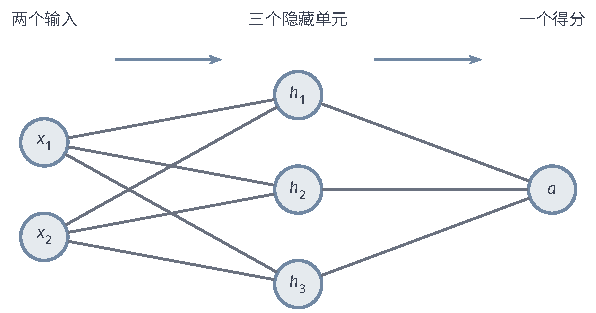
\includegraphics[width=100.993mm]{figures/03-models/02-neural-network-models/tikz/neural-minimal-mlp/figure.pdf}
  \caption{一个$2$-$3$-$1$多层感知机。两项输入先变成三个隐藏数值，再组合成一个分类得分。细线表示带权连接，箭头标出从左到右的计算方向；三个隐藏单元各作一次非线性变换，所有计算单元的偏置均省略。图只规定结构，权重尚未指定，也不要求某个隐藏单元预先代表某一种邮件特征。}
  \label{fig:neural-minimal-mlp}
\end{figure}
\FloatBarrier

围绕这个小网络，可以把学习中的三个问题分开。\term{表示能力}关心是否存在一组权重，使三个隐藏数值帮助输出端区分目标邮件；改变隐藏单元数，也会改变可选的计算。\term{优化}关心怎样根据训练邮件及其标签调整这些权重，让损失降低。\term{泛化}则关心训练后固定权重，面对未参与训练的新邮件时是否仍能作出可靠判断。这张图只给出了可执行的计算结构。若两项输入统计量已经丢失词序或否定关系，任何隐藏层也无法从相同输入中恢复这些区别；若输入保留了任务所需的信息，隐藏层才有机会把它变成适合预测的表示。

\subsection{特征变换与函数复合}
\label{sec:neural-feature-composition}

线性得分是否够用，取决于它作用在哪种表示上。设输入为$\bm{x}\in\mathbb{R}^{d}$，预先确定的特征变换为$\bm{\phi}:\mathbb{R}^{d}\to\mathbb{R}^{m}$，线性得分可以写成
\begin{equation}
  f(\bm{x})=\bm{w}^{\top}\bm{\phi}(\bm{x})+b,
  \label{eq:neural-fixed-features}
\end{equation}
其中$\bm{w}\in\mathbb{R}^{m}$是权重，$b\in\mathbb{R}$是偏置。即使得分对$\bm{\phi}(\bm{x})$是线性的，只要特征变换包含平方、乘积等运算，它对原始输入也可以是非线性的。困难因而不只在分类器，还在于如何找到适合任务的$\bm{\phi}$。

神经网络把固定的特征变换换成带参数的变换。沿用前文的\term{表示学习}（representation learning）概念，这意味着模型从数据中学习供后续任务使用的信息形式，而不只学习最后的预测权重。将表示变换记为$\bm{r}_{\bm{\theta}}:\mathbb{R}^{d}\to\mathbb{R}^{m}$，输出映射记为$g_{\bm{\psi}}$，完整预测函数为
\begin{equation}
  f_{\bm{\theta},\bm{\psi}}(\bm{x})
  =g_{\bm{\psi}}\!\left(\bm{r}_{\bm{\theta}}(\bm{x})\right),
  \label{eq:neural-representation-readout}
\end{equation}
其中$\bm{\theta}\in\mathbb{R}^{p}$和$\bm{\psi}\in\mathbb{R}^{q}$分别收集表示部分与输出部分的参数，$p,q$是相应参数量。对于标量得分，$g_{\bm{\psi}}$可以仍是线性函数；它现在作用于模型自己构造的表示。

表示部分通常由若干次变换组成。以具有$L$个表示层的网络为例，令$\bm{h}^{(0)}=\bm{x}$，第$\ell$层的输出为$\bm{h}^{(\ell)}\in\mathbb{R}^{d_\ell}$，其中$d_0=d$。一种常见计算形式是
\begin{equation}
  \begin{aligned}
    \bm{h}^{(\ell)}
      &=\sigma_\ell\!\left(\bm{W}_\ell\bm{h}^{(\ell-1)}+\bm{b}_\ell\right),
      \qquad \ell=1,\ldots,L,\\
    \bm{r}_{\bm{\theta}}(\bm{x})&=\bm{h}^{(L)},
  \end{aligned}
  \label{eq:neural-layer-composition}
\end{equation}
其中$\bm{W}_\ell\in\mathbb{R}^{d_\ell\times d_{\ell-1}}$、$\bm{b}_\ell\in\mathbb{R}^{d_\ell}$分别是权重矩阵和偏置向量，$d_L=m$。本式中的$\sigma_\ell$逐坐标作用，称为\term{激活函数}（activation function），即在加权组合之后改变单元输出的函数。每个单元产生一个坐标；图~\ref{fig:neural-minimal-mlp}中的三个隐藏数值，就是这里$L=1$、$d_1=3$时的$\bm{h}^{(1)}$。

式\eqref{eq:neural-layer-composition}把函数复合落实为逐层计算：上一层的输出就是下一层的输入。若各层激活函数都是恒等函数，两层变换合起来为
\[
  \bm{W}_2(\bm{W}_1\bm{x}+\bm{b}_1)+\bm{b}_2
  =(\bm{W}_2\bm{W}_1)\bm{x}+\bm{W}_2\bm{b}_1+\bm{b}_2\text{。}
\]
结果仍是一次仿射变换，即线性变换加偏置。重复叠加这种层不会改变这一性质。非线性激活使不同输入范围能够产生不同响应，才让多层组合有机会表达原始坐标中的复杂关系。

\begin{example}[异或的表示变换]
  \label{ex:neural-xor-representation}
  考虑四个二值输入$\bm{x}=(x_1,x_2)^{\top}\in\{0,1\}^{2}$，目标在两个坐标不同时为$1$、相同时为$0$，这就是\term{异或}（exclusive OR, XOR）。设正类由$w_1x_1+w_2x_2+b>0$确定。若四个点都被正确分类，必须同时满足
  \[
    \begin{aligned}
      b&\leq0,& w_1+w_2+b&\leq0,\\
      w_1+b&>0,& w_2+b&>0\text{。}
    \end{aligned}
  \]
  第一行来自两个负例，第二行来自两个正例。两条正类约束相加得到$w_1+w_2+2b>0$，两条负类约束相加却得到同一表达式不大于$0$，所以这样的线性得分不存在。

  令$\rho(a)=\max\{0,a\}$，它保留非负值、把负值置零，称为\term{整流线性单元}（rectified linear unit, ReLU）的激活函数。构造两个隐藏单元
  \begin{equation}
    h_1=\rho(x_1-x_2),\qquad h_2=\rho(x_2-x_1),
    \label{eq:neural-xor-hidden}
  \end{equation}
  则四个输入的表示依次为
  \[
    \begin{aligned}
      (0,0)&\mapsto(0,0),& (1,1)&\mapsto(0,0),\\
      (1,0)&\mapsto(1,0),& (0,1)&\mapsto(0,1)\text{。}
    \end{aligned}
  \]
  在新表示中，用$h_1+h_2>1/2$判断正类就能全部分对。这组参数是为说明机制而手工构造的，并非一次训练的实验结果；它证明了隐藏表示可以解决原始坐标中的线性不可分问题。
\end{example}

图~\ref{fig:neural-xor-representation}给出这个例子的几何读法。变换没有修改标签，而是把两个负例送到同一个位置，把两个正例留在另外两个位置。输出层因此可以采用简单的分界。表示不必保留输入的每一项区别；在这个任务中，区分$(0,0)$和$(1,1)$并不是得到正确标签所必需的信息。

\begin{figure}[htbp]
  \centering
  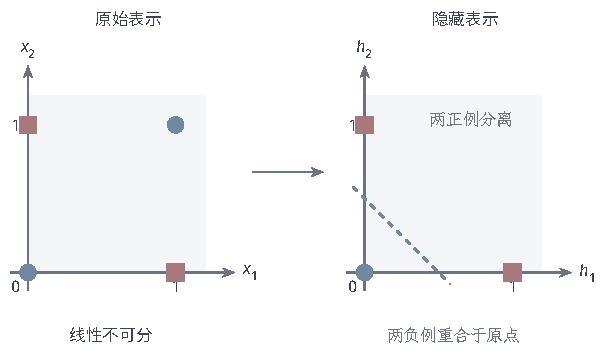
\includegraphics[width=102.902mm]{figures/03-models/02-neural-network-models/tikz/neural-xor-representation/figure.pdf}
  \caption{异或任务在变换前后的表示。圆点是标签为$0$的负例，方点是标签为$1$的正例。左侧两类点交错，无法用一条直线分开；右侧按式\eqref{eq:neural-xor-hidden}变换后，两个负例重合，虚线$h_1+h_2=1/2$将两类分开。坐标和变换均为教学构造。}
  \label{fig:neural-xor-representation}
\end{figure}

实际学习时，我们并不知道应该使用式\eqref{eq:neural-xor-hidden}中的权重。给定训练样本$S=((\bm{x}_i,y_i))_{i=1}^{n}$和损失函数$\ell$，可以把表示参数与输出参数放入同一个经验风险目标：
\begin{equation}
  \min_{\bm{\theta},\bm{\psi}}
  \frac{1}{n}\sum_{i=1}^{n}
  \ell\!\left(g_{\bm{\psi}}(\bm{r}_{\bm{\theta}}(\bm{x}_i)),y_i\right)\text{。}
  \label{eq:neural-joint-learning}
\end{equation}
两部分参数共同受最终任务的损失约束。这种\term{端到端学习}（end-to-end learning）把从输入到输出的一整条计算路径纳入同一学习目标。它仍需确定输入编码、网络结构和损失；对于不可微的操作，也需要另外设计参数更新方法。隐藏层能够表达有用特征、算法能够找到这些特征、得到的预测能用于新样本，是三个不同问题。

\subsection{分布式表示与层次表示}
\label{sec:neural-distributed-hierarchical}

一个隐藏向量有多个坐标，信息可以怎样放进这些坐标？如果每种对象只激活一个专属坐标，表示的区分主要由“哪一个坐标被激活”完成。\term{分布式表示}（distributed representation）采用另一种组织方式：一个对象由多个单元的活动共同表示，而同一个单元又可以参与多个对象的表示。这里的“分布式”指信息分布在若干坐标中，与把计算分配到多台机器是不同的概念。

一个简化例子是同时记录物体的颜色、形状和大小。若三个二值坐标分别表示“红色”“圆形”“较大”，那么$(1,1,0)$表示一个较小的红色圆形物体，$(1,0,0)$表示一个较小的红色非圆形物体。两个对象共享部分坐标，又在形状坐标上不同。三个二值坐标可以组成八种不同编码，说明共享属性能够通过组合区分对象；这只是编码数量的计算，不能据此推出模型用少量样本就一定能学会所有组合。

真实网络的坐标通常是连续数值，也未必逐一对应“颜色”这样的命名属性。表示中的信息可能需要若干坐标共同参与后续计算才能被读取。因而，某个单元响应某类输入，并不自动证明它只表示一个概念；分布式表示也可以是稀疏的，只要一个对象仍由若干可复用单元共同编码。这一区分允许表示同时复用多个坐标，而无需为每个对象指定一个独占单元\scite{goodfellow2016}

分布式表示考察同一层内的信息怎样分配，\term{层次表示}（hierarchical representation）则考察不同层之间怎样组合信息：后层利用前层的表示继续构造新特征。以图像为例，一层可以响应局部明暗变化，后层再组合这些响应以识别纹理或形状。这里的“局部变化—组合模式”是理解层次结构的一条路径，不是所有网络必须遵循的固定语义顺序。层数越多，也不保证每一层的含义越抽象或越容易解释。

两种表示方式可以同时存在。一个层用多个单元共同表达某种形状，下一层再把这组活动与其他信息组合。图~\ref{fig:neural-representation-path}强调的正是这种计算关系：每层提供一组供后续使用的数值，最终预测又通过学习目标影响各层参数。表示是否有用，要结合后续任务判断；为了分类而压缩的区别，在重建输入时可能仍然需要保留。

\begin{figure}[htbp]
  \centering
  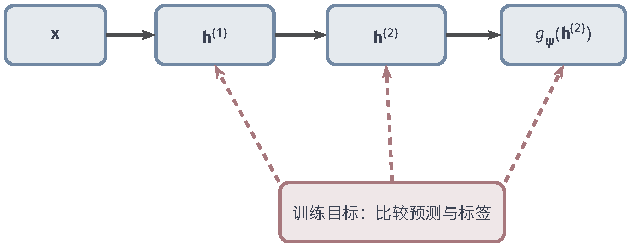
\includegraphics[width=106.793mm]{figures/03-models/02-neural-network-models/tikz/neural-representation-path/figure.pdf}
  \caption{表示学习的一条计算路径。实线表示输入经过两层变换后交给输出映射，虚线表示从训练目标返回的梯度或监督信号；它约束表示层与输出层的参数，但不是普通前向数据流。图只展示层间依赖，不要求隐藏坐标具有预先指定的语义。}
  \label{fig:neural-representation-path}
\end{figure}

\subsection{结构带来的归纳偏置}
\label{sec:neural-structural-bias}

允许学习表示，并没有规定所有输入都应怎样相互联系。若把图像中的每个像素与下一层所有单元相连，模型可以使用任意位置的组合，却没有直接体现相邻像素往往共同形成局部模式这一特点。网络结构可以预先限定哪些信息被组合、哪些计算被重复使用，从而影响学习时优先考虑的规律。

这种预先的限制或偏好称为\term{归纳偏置}（inductive bias）：面对有限数据，学习方法依据哪些假设把已经看到的关系推广到未见输入。偏置可以来自结构，也可以来自参数约束、损失和学习算法。这里聚焦结构，考察它怎样改变候选函数与信息传递路径。

\term{局部连接}（local connectivity）让一个单元只读取某个邻域的信息，例如图像中的一小块像素。\term{参数共享}（parameter sharing）让多个位置重复使用同一组参数，例如把同一个局部模式检测器移到图像各处。这两项设计分别规定“看哪些输入”和“在哪些位置使用同一种计算”。它们可以减少独立参数的数量，并使不同位置的数据共同参与共享参数的学习；具体效果仍取决于数据是否具有相应的局部性和重复规律。

对序列而言，结构还可以保留\term{隐状态}（hidden state），即在处理当前输入时保存一组由历史输入计算得到的数值。下一步继续读取这组数值，就能利用此前的信息。例如，看到“虽然”之后，后续判断可能需要继续保留尚未完成的转折关系。状态的存在提供了记忆通道，但状态维度、更新方式和学习过程仍会限制实际能够保留的信息。

结构假设匹配数据时，学习算法无需为每个位置或时间步单独发现同一种关系。假设不匹配时，同样的限制也可能排除需要的函数：只允许狭小邻域交互，可能难以直接比较相隔很远的对象；强制不同位置使用同一参数，可能忽略位置本身的特殊意义。网络设计需要在表达能力、样本利用与计算成本之间作出取舍。
架构规定可选函数的范围，训练算法从中选出具体函数；二者分别影响表达能力和学习结果，结构名称本身不能给出泛化保证。相关理论见\BookChapterRef{chap:deep-learning-theory}{第二卷“基础、理论和可信性”的“深度学习的可学习性”章}。

\section{生物神经网络}
\label{sec:neural-biological-inspiration}

人工网络为什么借用“神经元”“连接”和“学习”这些名称？理解它们的来源，需要同时看细胞怎样通信、系统怎样组织信息，以及经验怎样改变连接。本节从这三个方面介绍生物神经网络，再比较人工网络保留了哪些计算思想、哪些细节需要另外建模。

\subsection{神经元}
\label{sec:neural-biological-unit}

生物\term{神经元}（neuron）是接收和传递信号的细胞。许多神经元通过树突和胞体接收输入，\term{膜电位}（membrane potential），也就是细胞膜内外的电势差，随输入和细胞内部动态变化。在适当条件下，神经元产生称为\term{动作电位}（action potential）的短暂电信号，通常也称脉冲，并沿轴突影响其他细胞。神经元之间传递影响的连接部位称为\term{突触}（synapse），其传递效果可以随活动发生变化。这里概括的是典型脉冲神经元的部分机制，不覆盖所有细胞类型和信号传递方式。

图~\ref{fig:neural-biological-neuron}用一个神经元连接另外两个神经元的回路，把接收与传递信号的结构展开。树突从胞体向外分支，提供与其他细胞发生交互的部位；轴突则把信号传到末梢，末梢可以与其他细胞形成突触。支持神经元活动的\term{胶质细胞}（glial cell）参与维持细胞环境和形成髓鞘等过程。部分轴突外包有\term{髓鞘}（myelin sheath），即胶质细胞形成的多层膜结构，有助于加快传导。相邻髓鞘段之间的间隙称为\term{郎飞结}（node of Ranvier），动作电位在这些位置再生。在脑中，髓鞘由少突胶质细胞形成；神经元的形态各异，也并非所有轴突都有髓鞘\scite{purves2001}

\begin{figure*}[!t]
  \centering
  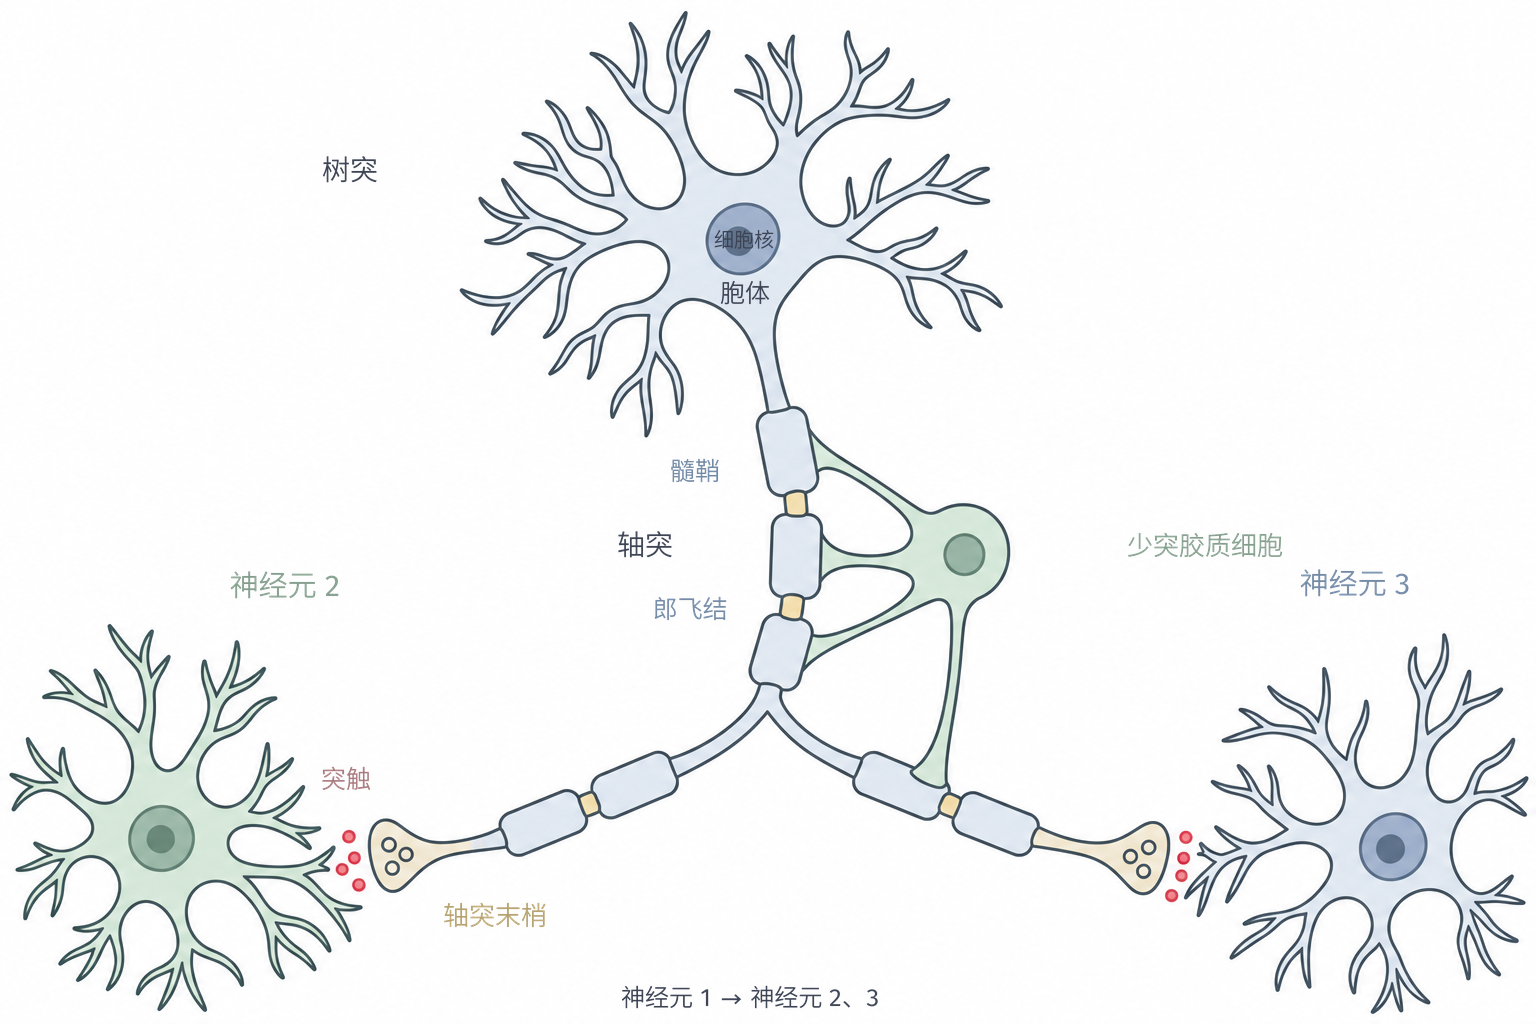
\includegraphics[width=130.048mm]{figures/03-models/02-neural-network-models/generated/neural-biological-neuron/figure.png}
  \caption{三个神经元在同一幅画面中通过突触相连。细线标出树突、胞体、细胞核、轴突、髓鞘、郎飞结与轴突末梢；神经元1的轴突分成两支，末梢分别与神经元2和神经元3形成突触，表示一个细胞可以向多个细胞传递信号。突触处的微小间隙只作概念提示。图展示一种多极、有髓鞘的神经元形态，各部分不按比例；真实神经元形态多样，部分轴突没有髓鞘，回路也可以包含反馈和更多连接。}
  \label{fig:neural-biological-neuron}
\end{figure*}

信号到达末梢后，怎样影响下一个细胞？在常见的\term{化学突触}（chemical synapse）中，动作电位促使末梢释放\term{神经递质}（neurotransmitter），即传递影响的化学信号分子。递质穿过两细胞之间的狭小间隙，与接收侧的受体作用，进而改变离子通道活动和膜电位。输入的作用可以是促进，也可以是抑制脉冲发放，具体取决于受体、通道与细胞状态。\term{电突触}（electrical synapse）则通过连接两细胞的通道直接传递电流。因此，图中的连接不能统一理解成把一个数值无延迟地送给下一个单元的导线\scite{purves2001}

接收到一次输入，并不意味着细胞必然发放一次脉冲。突触输入引起的膜电位变化会持续一段时间，再逐渐衰减；若其他输入在这段时间内到达，它们的影响就可能共同改变细胞的响应。来自多个连接的输入与同一连接在不同时间到达的输入，都可以参与这种整合，抑制性输入又可能降低发放的机会。在简化模型中，可以把较弱输入的影响近似相加，并用阈值描述何时发放；真实细胞的整合还取决于树突位置、膜上的通道和近期活动，未必只是一个静态加权和\scite{gerstner2014}

\Needspace{6\baselineskip}
脉冲的个数与发生时刻都可以参与信息表达。例如，同样发放3次脉冲，集中在短时间内与分散在较长时间内，对接收细胞可能产生不同影响；单个细胞的活动又需要放在其他细胞的共同活动中理解。许多典型动作电位持续约$1$至$2\,\mathrm{ms}$，这是细胞信号的时间尺度，不能直接当作大脑完成一个判断所需的时间。判断可能依赖多个回路中的持续活动与往返交互\scite{gerstner2014}

\FloatBarrier
\subsection{神经系统}
\label{sec:neural-biological-system}

单个细胞的接收和发放机制，还不能解释视觉、记忆或动作怎样形成。神经元连接成局部回路，多个回路再参与更大范围的神经系统。按解剖位置，人类神经系统通常分为脑与脊髓组成的\term{中枢神经系统}（central nervous system, CNS），以及联系中枢与身体其他部分的\term{外周神经系统}（peripheral nervous system, PNS）。感觉输入、内部活动和动作输出通过这些系统相互联系；下面主要考察人脑，尤其是与人工视觉模型联系较紧密的大脑皮层\scite{purves2001}

脑中细胞数量及其分布提供了理解回路规模的依据。Azevedo等在2009年分析了4个年龄为50至71岁的成年男性脑样本，估计神经元数量的样本均值约为$861$亿，样本标准差约为$81$亿。这是常用的“人脑约有860亿个神经元”说法的一项主要依据。研究通过细胞核计数与神经元标记估算数量；这个结果应当用于理解规模，不能当作每个人都有同样数量的精确常数。同一研究中，大脑皮层约有$163$亿个神经元，小脑约有$690$亿个，分别约占总数的$19\%$和$80\%$。神经元数量在不同结构间很不均匀，数量最多的结构也不能仅凭这一点被认定为负责所有最复杂的认知任务\scite{azevedo2009}

这些细胞并非排成一组统一的层。脑内既有形成局部回路的连接，也有联系不同区域的长距离通路；大脑皮层、小脑和脑干等结构具有不同的细胞组织与连接方式。神经元与胶质细胞共同构成脑组织，后者还参与代谢支持等过程。因而，理解脑的架构，需要同时考察细胞类型、局部回路与区域间通信，不能只数计算单元\scite{purves2001}

数量与连接给出结构，网络活动才描述这套结构如何处理信息。大量细胞可以同时接收输入和改变状态，计算分散在许多局部回路中；反馈连接又使当前响应依赖过去的活动。即使没有新的外部任务，脑内仍有持续的活动。并行性、内部状态与信号往返让脑能够处理随时间变化的感觉和行为信息，但这些特点本身不能给出某项任务的准确率，也不能由细胞数量推出每秒完成多少次通用算术运算。

维持这种活动还需要能量。成人脑的质量约占体重的$2\%$，却消耗全身约$20\%$的氧和相应代谢能量\scite{raichle2002}描述成人脑时，约$20\,\mathrm{W}$这一量级常用于表示葡萄糖供能对应的代谢功率；它包含通信与维持细胞功能等支出，各过程如何分摊能量还依赖具体的估算模型\scite{levy2021}这说明信息传递和维持活动也是计算系统的成本。若要与人工系统比较效率，需要固定任务、准确率、响应时间和能耗范围；把一次突触事件直接算作一次浮点运算，会忽略两者操作内容和精度的差异，得不到统一的“大脑算力”。

\FloatBarrier
这些局部回路和长距离连接在皮层中怎样组织？\term{大脑皮层}（cerebral cortex）是覆盖大脑半球表面的薄层组织，折叠形成沟和回。皮层属于\term{灰质}（gray matter），其中集中着细胞体、树突、突触与局部轴突；皮层下的\term{白质}（white matter）以轴突束为主要组成，为区域间通信提供通路。两种名称概括组织组成，并不是把脑机械分成“只计算”和“只传输”的两部分\scite{purves2001}

人脑大部分皮层属于\term{新皮层}（neocortex），按细胞密度、形态和连接等特征，通常从表面向内分成I至VI六个解剖层。不同层接收与发出的连接有所不同，层内存在横向联系，层间又有跨层联系。这里的“六层”是同一片皮层厚度方向上的组织分层；V1、V2等脑区各自包含自己的层内和层间回路，不能把这六层理解成人工网络连续执行的六个计算步骤\scite{purves2001}

层内与层间回路还与其他区域相连。以视觉为例，可以观察局部输入怎样经过多个区域，形成识别和行动所需的信息。\term{中央沟}（central sulcus）是区分额叶与顶叶的主要解剖标志，本身不是视觉计算阶段。图~\ref{fig:neural-visual-pathways}借助各叶的位置定位视觉区，箭头表示主要传递方向。

视觉处理从眼中的\term{视网膜}（retina）开始，光在这里转化为神经信号，并经过局部回路处理。一条主要通路把视网膜神经节细胞的输出经丘脑的\term{外侧膝状体}（lateral geniculate nucleus, LGN）送到\term{初级视觉皮层}（primary visual cortex, V1）。V1主要位于枕叶内侧的距状沟周围，单从脑的外侧看不到它的大部分。V1之后的信号经V2等区域继续传递，逐渐进入分布在枕叶、颞叶与顶叶的多个视觉区域。这里描述的是主通路，视觉信号也参与眼动和反射等其他通路\scite{purves2001}

\begin{figure*}[!t]
  \centering
  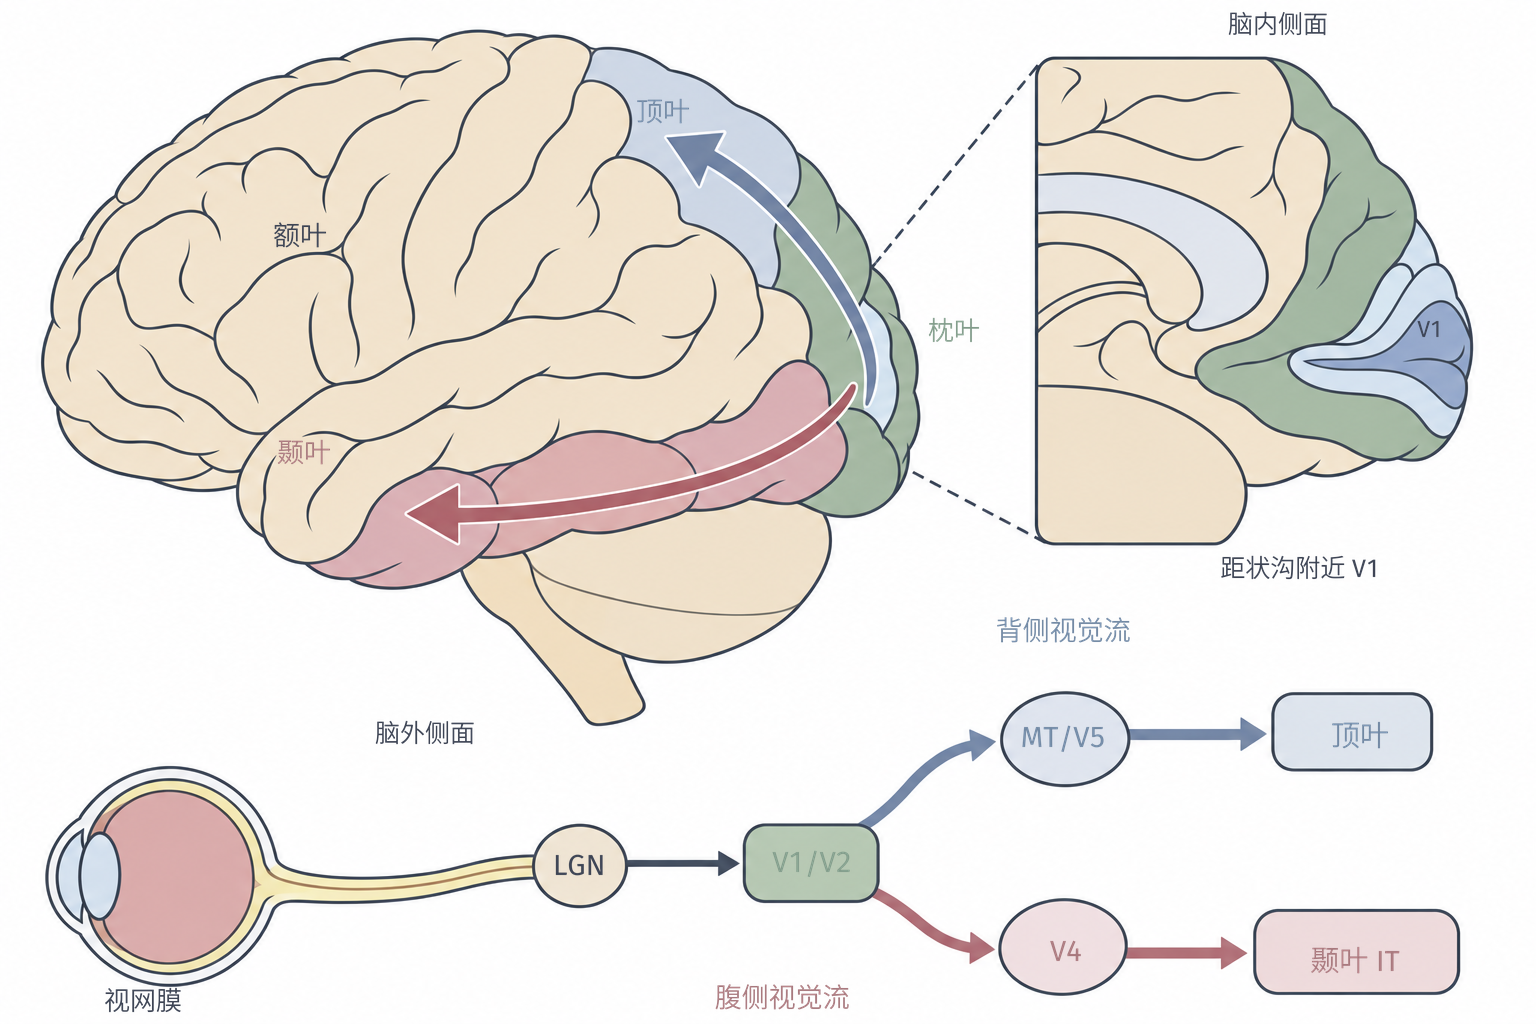
\includegraphics[width=130.048mm]{figures/03-models/02-neural-network-models/generated/neural-visual-pathways/figure.png}
  \caption{人脑视觉区域的位置与两条主要通路。外侧解剖插画标出各脑叶，内侧图标出距状沟附近的V1；两条彩色路径概括视觉信息向顶叶和颞叶传递的方向。下方路径图从视网膜和LGN进入V1/V2，再以蓝色表示经MT（V5）向顶叶传递的空间通路where，以红色表示经V4向IT传递的内容通路what。区域与箭头依据视觉区研究和通路概括绘制，不表示精确边界、完整连接或唯一串行顺序；跨通路联系与反馈未画全。}
  \label{fig:neural-visual-pathways}
\end{figure*}

图中的区域名并非一张“每区只负责一个属性”的清单。V3是早期视觉区域之一，含有背侧与腹侧部分；V4及人脑常用的hV4名称关联于腹侧视觉区，其中的响应涉及颜色与形状等信息。MT也常称V5，运动相关响应是识别它的一项重要线索；人脑成像中的hMT+还可以包括邻近的运动相关区域，不能把这些名称当作边界完全相同的单一区域。\term{下颞皮层}（inferotemporal cortex, IT）指下部颞叶的一组视觉相关皮层，是理解物体识别通路的区域性称谓。人脑与其他灵长类的视觉区域在命名和边界上存在差别，图中保留V4、MT、IT等常见名称用于讲解，不声称它们在所有物种中逐一相同\scite{wandell2007}

区域间的联系通常概括为两条主要通路。\term{腹侧视觉通路}（ventral visual stream）从早期视觉区向V4等区域以及下颞皮层传递信息，偏重颜色、形状与物体身份，因此常称\term{内容通路}（what pathway），即帮助判断“看到的是什么”。\term{背侧视觉通路}（dorsal visual stream）联系MT、其他背侧视觉区与后部顶叶皮层，偏重运动、空间关系和视觉引导的动作，常称\term{空间通路}（where pathway）。例如，看到一个杯子时，识别它是杯子与确定伸手抓取时的位置、方向和手形，需要利用不同但相互配合的信息。where并不只表示报告静态坐标，也包含如何根据视觉控制动作；两条通路之间还会交换信息\scite{goodale1992}

\FloatBarrier
这些区域为何适合启发层次模型，还要回到单元响应。一个视觉神经元通常只对视野中某个范围内的刺激产生相应变化，这个范围称为\term{感受野}（receptive field）。感受野说明“哪些位置的输入能影响该单元”，单元的响应偏好则说明“这些位置上出现什么模式时响应更强”。Hubel和Wiesel在猫的视觉皮层中研究了对特定取向的光条或边缘敏感的细胞，并区分简单细胞与复杂细胞的感受野特征。简单细胞对亮暗位置的安排具有较明确的选择性，一些复杂细胞则能在一定位置范围内对相近取向的刺激作出响应。这些实验为局部响应及其组合提供了生物学依据；实验对象是猫，不能把全部细节直接当作人脑的逐层结构\scite{hubel1962}

局部响应经过后续回路组合，可以对更大范围、更复杂的模式产生选择性：早期视觉区中的取向信息与后续区域中的形状、物体相关响应，共同提供了理解\term{层次特征}（hierarchical feature）的生物学线索，即利用已有特征继续形成新的特征。这里的层次跨越多个回路和区域，与皮层的六个解剖层属于不同概念。视觉连接还包含反馈和并行通路，因此“局部边缘—形状—物体”适合作为理解线索，不能当作大脑必须逐步执行且只执行一次的流程\scite{purves2001}

\subsection{生物学习}
\label{sec:neural-biological-learning}

视觉回路能够组合已有响应，但经验还需要改变以后面对输入时的响应。短暂的膜电位变化描述细胞当前的状态；较持久的连接变化则能改变后续输入产生的影响。\term{突触可塑性}（synaptic plasticity）指突触传递效果能够随活动等因素改变，是研究生物学习的一类重要机制。

先看只依赖连接两端活动的简化规则。用标量$w_j$概括第$j$条连接的强度，用$u_j$和$h$分别概括输入端与输出端的活动，一个相关性更新例子是
\begin{equation}
  \Delta w_j=\eta u_j h,
  \label{eq:neural-local-correlation}
\end{equation}
其中$\Delta w_j$是连接强度的改变量，$\eta>0$控制更新幅度。这个式子展示一种\term{赫布学习}（Hebbian learning）思路：共同活动影响连接强度。它是便于比较的信息依赖示例，没有脉冲时序、权重限制和整体任务误差，不能当作完整生物学习机制；若持续出现正相关活动而没有其他约束，权重还可能不断增大。

相关活动还可以细分为发放的时间关系。\term{脉冲时序依赖可塑性}（spike-timing-dependent plasticity, STDP）描述突触变化对两端脉冲相对时刻的依赖。Bi和Poo在培养的海马神经元中观察到，特定配对条件下，突触变化与脉冲先后关系有关；该结果描述的是相应细胞和实验条件，不能直接扩成所有突触的统一规则\scite{bi1998}

局部相关性还没有解决“怎样改变连接才能改善行为”这个问题。例如，伸手抓取杯子时动作出现偏差，需要把行为结果与参与感觉和动作的多个回路联系起来。这种\term{信用分配}（credit assignment）问题关心整体结果的好坏应怎样影响内部各个环节。仅仅知道两端曾经共同活动，并不足以确定这条连接对行为偏差的贡献。生物可塑性还受到反馈和调节信号的影响，局部变化如何与整体目标联系，仍是研究的重要问题\scite{lillicrap2020}

\subsection{与人工神经网络的对比}
\label{sec:neural-biological-comparison}

生物细胞、回路和可塑性为人工模型提供了不同层次的启发。比较时需要明确当前关注的是输入与输出的函数关系、信号的时间动态，还是学习规则；同一个模型可以在某一方面相似，在另一面采用工程上的简化。

人工计算单元保留了“多个输入共同影响输出”这一抽象。若输入为$\bm{u}\in\mathbb{R}^{d}$，单元可以写为
\begin{equation}
  a=\sum_{j=1}^{d}w_j u_j+b,\qquad h=\sigma(a),
  \label{eq:neural-artificial-unit}
\end{equation}
其中$w_j$描述第$j$项输入对加权和$a$的影响，$b$调整响应的位置，$\sigma$把$a$映射为输出$h$。权重对应的是连接影响强弱的数学抽象，激活函数对应的是输入与输出之间的响应关系；二者都没有完整描述突触化学过程或细胞电生理。

图~\ref{fig:neural-unit-abstraction}把人工单元的运算展开：每项输入乘以相应权重，所有贡献与偏置相加，再经过激活函数。这种画法便于逐项核对式\eqref{eq:neural-artificial-unit}，却已经省略了图~\ref{fig:neural-biological-neuron}中的细胞形态与化学过程。该式也没有内部时间状态，因此仅凭当前$\bm{u}$就能计算$h$；一个真实细胞的响应还可能依赖此前的膜电位、近期活动和其他调节因素。这一差别决定了普通单元适合哪种抽象，也为后文保留时间动态的脉冲模型留下了空间。

\begin{figure}[htbp]
  \centering
  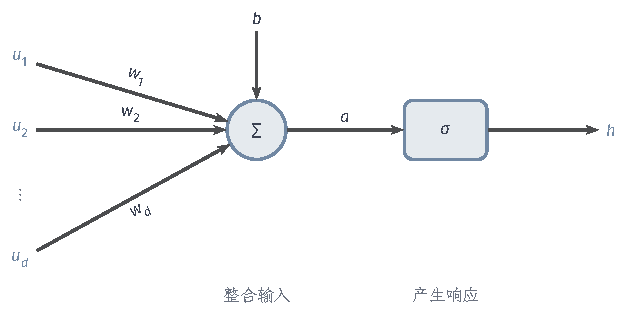
\includegraphics[width=106.161mm]{figures/03-models/02-neural-network-models/tikz/neural-unit-abstraction/figure.pdf}
  \caption{人工神经元的计算示意。标有$w_j$的输入边表示乘以权重，求和节点再加入偏置$b$，激活函数产生输出$h$。接收输入、整合影响与产生输出，是它与生物神经元之间的功能对应；图中的数学运算不完整复现细胞机制。}
  \label{fig:neural-unit-abstraction}
\end{figure}

\Needspace{10\baselineskip}
多个单元连接起来，比较的对象便从细胞变为网络。图~\ref{fig:neural-biological-artificial-networks}左侧用局部回路与跨区域连接表示生物组织的一些特点，右侧则给出一个明确的层状前馈计算。右图的中间输出按约定次序计算，左图所示回路则可以让此前活动再次影响后续响应。人工网络也可以加入反馈、状态和不同单元类型；二者的区别需要落实到具体结构与动态，而不能只看图上都有节点和连线。一个生物神经元可以具有复杂的树突计算，一个人工单元也可以被设计成复杂函数，因此神经元数、人工单元数与参数量不能直接互换。

\begin{figure*}[htbp]
  \centering
  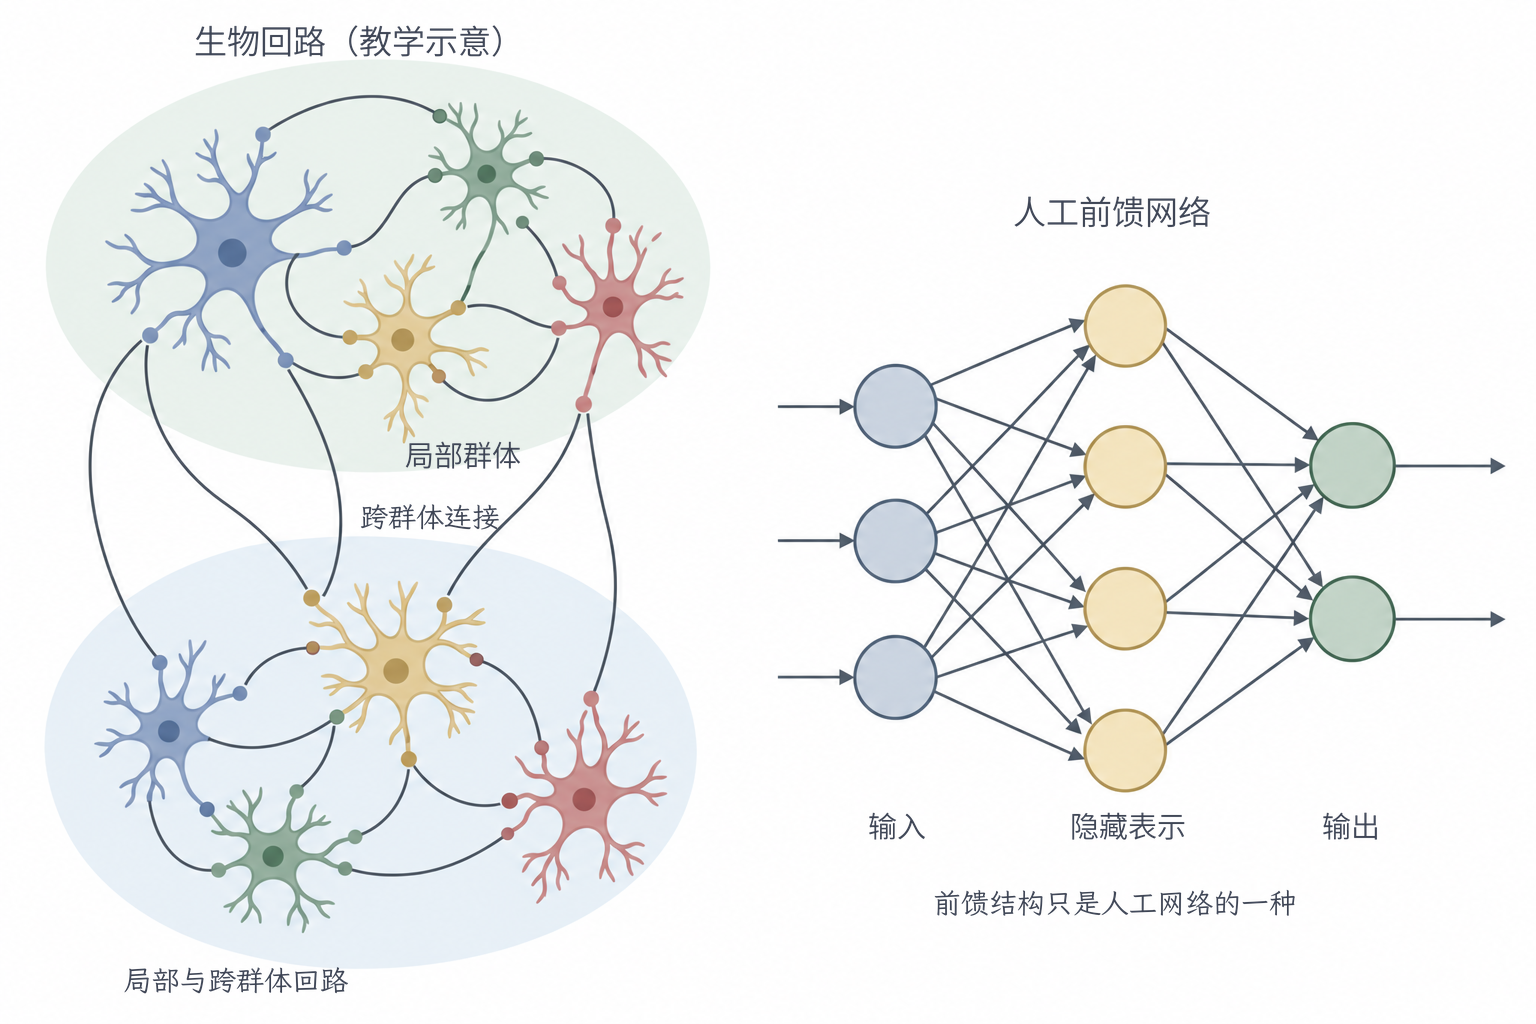
\includegraphics[width=130.048mm]{figures/03-models/02-neural-network-models/generated/neural-biological-artificial-networks/figure.png}
  \caption{从单元到网络的两种组织示意。左侧用轮廓不同的节点表示细胞类型差异，淡色区域表示局部群体，箭头同时包含局部回路与跨群体联系；它是教学构造，并非测得的人脑连接图。右侧是一个前馈人工网络，箭头表示输入、中间表示与输出之间的计算依赖。图中的节点数量不表示真实规模，右图也不涵盖人工网络的所有结构。}
  \label{fig:neural-biological-artificial-networks}
\end{figure*}
\FloatBarrier

前面介绍的视觉感受野与层次响应，带来了一个人工视觉模型的设计问题：能否在不同位置检测局部模式，再把这些检测结果组合成更大范围的表示？Fukushima在1980年提出的\term{新认知机}（neocognitron）受这种层次思路启发，交替组织检测局部模式的S单元与汇集响应的C单元，以获得对位置变化具有一定容忍度的识别表示。这是从视觉机制走向人工层次结构的一项早期工作，其自组织学习方法也与后来的监督梯度训练不同\scite{fukushima1980}

卷积神经网络沿用的核心设计包括局部感受野、重复使用局部检测方式，以及逐层扩大信息组合范围。局部连接限制一个单元读取的输入区域；参数共享则把同一个检测函数用于不同位置。后者是明确的工程约束，不能从“许多生物细胞具有相似响应偏好”推出它们精确共享同一组突触参数。网络还可以采用\term{池化}（pooling），即汇总邻域内的若干响应，以降低表示的空间分辨率或减小对局部位移的敏感性。卷积、非线性响应与邻域汇总组合后，后层能够读取较大范围内的局部特征组合。

局部检测与后续组合，为卷积网络从图像局部结构构造表示提供了设计依据。人工卷积层与视觉脑区之间没有由此确定的一一对应关系。what与where也区分了表示服务的目标：物体识别希望在位置变化后仍保留身份判断，定位和动作控制却需要保留空间关系，不能一概消除位置信息。感受野、参数共享和池化怎样改变信息，以及何时保持平移等变或得到位置不变的输出，将在卷积神经网络章写成明确运算。这里的生物学关联解释设计动机，运算性质则取决于具体结构。

\term{脉冲神经网络}（spiking neural network, SNN）把单元之间传递的信号表示为离散脉冲事件，并通常保留随时间演化的内部状态。它既可用于研究神经系统，也可用于任务预测和事件驱动计算；连接结构、单元动态和参数学习规则还需要分别设计。

脉冲模型可以用输入改变膜电位、达到阈值时发放并重置状态等规则，保留“积累—发放”的时间过程；普通连续值单元则常直接计算当前输入对应的数值。这样的差别使SNN更适合表达某些脉冲时刻相关的问题，但脉冲编码不自动补齐树突形态、递质作用、胶质支持或生物可塑性。卷积与脉冲也不是互斥的网络类别：前者规定局部连接和参数共享，后者规定信号形式与时间动态，因而可以构造采用脉冲单元的卷积网络\scite{gerstner2014}

\paragraph{学习机制与信用分配}
在单元形式之外，更深的差别是怎样从经验中改变连接。常见的人工网络训练直接规定一个整体损失，并利用该损失对各参数的导数更新参数。对于式\eqref{eq:neural-artificial-unit}，设当前可微损失$\mathcal{L}$通过输出$h$依赖权重$w_j$，则
\begin{equation}
  \frac{\partial\mathcal{L}}{\partial w_j}
  =\frac{\partial\mathcal{L}}{\partial h}\,\sigma'(a)\,u_j\text{。}
  \label{eq:neural-unit-credit}
\end{equation}
输入$u_j$和局部导数$\sigma'(a)$只描述这个单元附近的计算；$\partial\mathcal{L}/\partial h$还包含$h$通过后续网络影响损失的信息。\term{误差反向传播}（error backpropagation）从输出端出发，沿计算依赖反向应用链式法则，组织这些导数的计算。它提供梯度；用梯度怎样修改参数，是优化算法的工作。若激活函数在某点不可微，则需另行约定该点的处理方式。

\Needspace{7\baselineskip}
两类学习的共同点，是经验能够改变连接的影响，进而改变下一次输入引起的响应。生物突触的传递效果与人工权重都承担了这种作用，许多连接的变化共同影响网络的行为。这里还需要区分当前活动与连接学习：一次脉冲或一次前向计算改变当前活动，连接学习则改变突触传递效果或模型参数。内部状态也可以保存信息，但状态变化与连接更新是不同的对象。这个对应解释了为什么人工网络可以借鉴可塑性，却没有规定两者必须使用同一种更新规则。

生物学习的重要基础是局部突触可塑性。通常所说的\term{赫布定律}（Hebb's rule）强调：一个神经元的活动反复参与另一个神经元的发放，两者之间的连接可能增强。式\eqref{eq:neural-local-correlation}展示的是这种思想的简化形式。不过，大脑的学习不能只写成“两端同时活动就增强连接”。脉冲时序、细胞状态与调节信号都会影响变化；一些研究还考察局部活动能否先留下短暂的突触痕迹，待奖励等信号到来时再改变连接。这使局部活动能够与稍后出现的行为结果联系起来，仍不等于逐条计算整体损失的精确梯度\scite{gerstner2018plasticity}

局部可塑性与标准反向传播的区别，具体落在更新信号及其传递方式上。标准反向传播把一个明确的任务损失作为共同依据：式\eqref{eq:neural-unit-credit}中的$\partial\mathcal{L}/\partial h$衡量隐藏输出如何影响最终损失，后续计算的导数又把这一影响传回当前单元。因此，即使两条连接附近的活动相似，只要它们对任务误差的贡献不同，得到的梯度也可以不同。式\eqref{eq:neural-local-correlation}仅使用两端活动，STDP则进一步利用脉冲的相对时刻；这些局部量本身没有给出最终任务损失的精确导数。用“活动相关”决定变化，与用“对任务误差的影响”决定变化，是本节两种更新示例最需要区分的地方。

学习信号的实现方式也不同。在常见的软件实现中，人工网络沿已知计算图反向求导，并在数值存储中更新参数；生物突触的变化由细胞内过程实现，能够使用的活动、时序及反馈信号受实际连接和动态限制。已有的反馈与可塑性研究尚不足以说明大脑执行标准反向传播；单一赫布规则也没有涵盖前面讨论的时序、状态与调节因素。大脑存在广泛反馈，研究仍需解释这些反馈怎样帮助信用分配。Lillicrap等讨论了利用反馈引起的活动变化近似误差信号的可能机制；这是关于可能实现方式的探索，尚不构成大脑执行标准反向传播的证据\scite{lillicrap2020}

上述差异针对本节比较的局部可塑性与标准反向传播，不是生物和人工系统的绝对分界。人工网络也可以采用局部相关性更新，脉冲网络也可以按任务损失训练。采用哪种编码、怎样连接单元、怎样学习参数，是需要分别说明的设计选择。

\paragraph{信息流动与自上而下的预测}
学习规则不同，还要与感知时的信息流区分开。在一个普通前馈分类器中，输入经过各层产生输出，一次预测不需要把高层结果再送回低层。人脑的视觉系统则同时存在自下而上的感觉输入和自上而下的反馈，当前理解会反过来影响对输入的处理。Bar等的研究支持一种具体假说：图像的粗略信息较快到达额叶中的眶额皮层，由这里形成可能的物体解释，再帮助颞叶视觉区域识别输入。研究观察到识别相关的眶额活动早于相应颞叶活动，这为预测参与视觉识别提供了依据；不能据此把所有预测都归结为额叶一个区域\scite{bar2006}

面对模糊物体时，已有经验可以帮助形成候选解释，再与当前感觉证据相互校正。日常所说的“脑补”可以从这种补全缺失信息的过程理解；预测可能帮助识别，也可能使错误预期干扰判断。感知中的反馈传递神经活动，反向传播计算训练所需的导数，两者的对象与用途不同。人工网络也能加入循环、反馈或反复推断，因此“人工信息流只有前向”只适用于这里比较的前馈结构，不能概括全部人工架构。

\paragraph{少样本学习与知识迁移}
人往往能利用少量新例子理解与已有经验相关的概念。例如，已经熟悉书写的人看到一个陌生字符，可以利用笔画、连接和书写方式来判断它的其他写法。Lake等以手写字符为对象研究单样本概念学习，并构造了能够组合和复用笔画等知识的程序模型；模型在相应任务上达到与人类相近的表现。这项结果说明，少量新样本可以与丰富的已有知识共同支持泛化，而不是证明人脑在毫无先前经验时也能学会任意任务\scite{lake2015}

从随机参数开始、只按当前任务标签训练的监督网络，需要从这一批训练数据同时获得内部表示和分类规则。迁移学习或元学习改变了这个知识起点：新任务的训练可以利用此前获得的表示、参数或适应规则。人工网络可以通过迁移学习复用已经学得的表示；元学习则利用多个训练任务，让参数或适应规则经过训练后能够用少量新任务样本调整\scite{finn2017}比较样本效率时，需要同时记录新任务用了多少样本，以及此前用了多少数据、任务和其他知识。人类的快速迁移是人工学习的重要参照，但新知识与旧知识的联系越弱，就越不能假定只需少量练习。

\paragraph{鲁棒性与对抗扰动}
在熟悉对象的识别中，人可以容忍一定程度的模糊、遮挡和背景变化。不过，普通图像上的高准确率并不保证人工网络也具有同样的感知稳定性。Szegedy等发现，针对网络寻找的细小图像扰动，可以在视觉上几乎不改变图像时使模型误分类\scite{szegedy2014intriguing}例如，可以出现人仍把图像看作一个杯子，分类器却输出另一类别的情形。这里的扰动经过有意搜索，与随意加入一点随机噪声不同；它暴露了模型的分类依据与人的判断之间的差距。

\Needspace{7\baselineskip}
上述例子限定了输入和分类器，也没有检验人在其他观察条件下是否会受到攻击影响。Elsayed等发现，在限制观察时间的实验条件下，一些针对计算机视觉系统构造的扰动也会影响人的分类\scite{elsayed2018humans}人类还会受到错误预期和跨感官冲突的影响。因此，比较鲁棒性应固定任务、扰动范围、观察时间和评价指标；人工网络的稳健训练也会改变结果。
普通噪声、自然分布变化与针对分类器有意搜索的扰动改变输入的方式不同，因而需要分别评价；其评价条件见\BookChapterRef{chap:trust-robustness}{第二卷“基础、理论和可信性”的“鲁棒性”章}。

\paragraph{计算活动的能量成本}
人脑在约$20\,\mathrm{W}$量级的代谢功率下，持续维持感觉、行动和内部活动，这种丰富功能与较低功率并存的现象构成了人工计算的重要参照。这个数字包含通信和维持细胞功能等成本，不能只算作“有用运算”的功率；脑内的信息传递本身也需要能量\scite{levy2021}典型数字实现中的人工网络则要执行数值运算，并在存储与计算部件之间读取权重和中间结果。模型大小、计算精度、活动是否稀疏以及数据搬运方式，都会影响实际能耗。

生物回路中的稀疏脉冲活动和局部连接为减少不必要的计算和通信提供了设计线索，但采用脉冲模型并不自动保证节能。比较时还要区分功率与能量：同样的功率，运行时间越长，总能量越多。因而，不能用整个人脑的代谢功率直接对比某块设备的额定功率，就得到每次判断的能效倍数；应固定任务与准确率，并计入响应时间、学习成本以及所测系统的范围。

\paragraph{多感官输入与联合处理}
听别人说话时，声波和说话者的口形同时提供线索。人脑可以联合处理这些输入，而不是等视觉和听觉各自给出最终答案后才简单拼接。这种\term{多模态处理}（multimodal processing）利用不同类型的信息通道共同理解同一事件。McGurk和MacDonald的经典实验表明，把一种音节的声音与另一种音节的口形配在一起，会使一些人报告听到第三种音节，说明视觉信息能够改变语音感知，而不只是给听觉附加一条独立说明\scite{mcgurk1976}

神经系统本身具有多种感觉通道及跨通道联系，具体整合能力仍会随发育和经验形成，不能把所有跨感官关联都理解为出生时已经成熟\scite{stein2014multisensory}许多人工模型只为一种输入类型设计，需要另外建立不同输入之间的联系；人工网络也能学习多模态表示。例如，图像与文本的联合训练可以把描述和图像关联起来\scite{radford2021}这里的差别在于系统能够利用哪些输入、哪些关联来自结构或经验，以及训练是否建立了这些关联，并非人工网络原则上只能处理单一模态。

模型保留哪些生物细节，由它要解释的现象决定。研究脉冲发生时刻，需要保留影响发放的动态；解释突触变化，需要让更新规则对应实验中的活动和配对条件。面向预测的人工网络则按任务输出评价，运行代价还取决于计算与实现。这些评价可以相互补充，但证据各有对象：复现某组神经响应说明模型能够产生相应活动，还需要学习过程的观察才能判断参数如何获得；预测正确也只说明相应任务上的输出符合目标。

\section{神经网络的类型}
\label{sec:neural-network-types}

“卷积”“循环”“图”“注意力”“脉冲”分别强调不同性质。将这些名称并排列出，容易误以为一个网络只能属于其中一类。本节按连接结构、信息交互方式和信息编码方式分别观察同一个计算对象；这些分类可以交叉，也不要求每个完整架构只使用一种机制。

\subsection{按连接结构划分}
\label{sec:neural-types-connectivity}

连接结构关心计算单元之间的依赖方向与组织方式。\term{前馈神经网络}（feedforward neural network）沿没有有向环的计算依赖，把输入逐步送到输出；同一次计算中的中间结果不再返回去修改自己的上游输入。式\eqref{eq:neural-layer-composition}是层状前馈网络，跨层连接也可以保持前馈性质，只要计算依赖仍然没有有向环。

\term{循环神经网络}（recurrent neural network, RNN）把此前状态用于下一次更新。同一组更新参数在多个时间步重复使用，因而既处理当前输入，也传递历史影响。固定输入序列并按时间展开后，每一步读取已计算出的前一步状态，得到的展开计算可以没有有向环；名称中的“循环”描述的是状态反馈与参数复用，不是要求在一个时间步中无限反复求值。

例如，判断一句评论是肯定还是否定，可以先把整句转为定长向量，再让前馈网络逐层得到分类得分；也可以让循环网络逐词读取评论。后一种结构在读到“不”后更新状态，读到“好”时同时使用当前词和此前状态，因而提供了保留否定关系的途径。前馈结构传递的是本次计算中已经得到的中间值，循环结构还显式传递跨时间步的状态；存在这条状态通道，并不保证训练后就一定记住了“不”。

依赖也可以沿树组织。\term{树递归网络}（recursive neural network）按照树中的父子关系递归地组合表示，例如用两个子树的表示形成父节点表示。链式状态更新每次通常接收一个前序状态，树递归则可能组合多个子节点状态，计算顺序和共享方式因此不同。本书采用广义的循环网络口径，把链式循环、树递归及基于隐状态递推的状态空间网络放在循环网络章讨论；它们的具体拓扑仍分别说明。

\term{图神经网络}（graph neural network, GNN）根据输入图中的实体和关系组织表示计算，例如让一个节点读取相邻节点的信息。这里必须区分输入图与网络的计算依赖：输入图可以有环，模型却可以只执行固定轮数的同步更新，时间或轮次展开后仍得到有限的计算过程。另一类图网络通过反复状态更新求取某种稳定状态，两者的学习和计算条件不同。

以预测路口拥堵为例，输入节点可以是路口，边表示道路连接。一次同步更新让每个路口读取上一轮的邻居车流表示，再生成自己的新表示。即使道路形成环路，这一轮也不用等待邻居先算出同一轮的新值；按轮次保存旧值与新值，就能执行有限次更新。

图~\ref{fig:neural-topologies}将三个常见依赖模式放在一起。前馈图说明层间先后，链式展开说明状态的跨时间依赖，输入图则说明哪些实体有关联。每个神经网络都能用计算图描述，不意味着每个网络都是图神经网络；后者的“图”特指模型利用输入的关系结构来组织计算。

\begin{figure}[htbp]
  \centering
  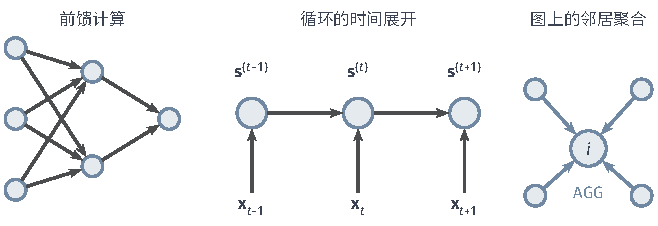
\includegraphics[width=111.361mm]{figures/03-models/02-neural-network-models/tikz/neural-topologies/figure.pdf}
  \caption{三种不同对象的结构示意。左侧是前馈计算中的单元依赖；中间是循环更新的时间展开，三个更新位置共享同一组状态更新参数；右侧显式画出图神经网络的一次邻居聚合，蓝色邻居沿箭头向中心节点$i$提供消息。输入关系可以有环，但一次同步更新的计算依赖仍按层推进。}
  \label{fig:neural-topologies}
\end{figure}
\FloatBarrier

\subsection{按信息交互方式划分}
\label{sec:neural-types-interaction}

确定了大体依赖后，还需说明一次更新怎样组合信息。\term{全连接}（fully connected）让一组输出中的每个单元读取上一组的全部坐标，常用一个稠密矩阵完成加权组合。\term{卷积}（convolution）则按规则网格读取局部邻域，并在不同位置重复使用同一组参数。全连接提供广泛的坐标组合，卷积把局部性与位置间复用直接写进运算；它们既可以构成完整网络，也可以成为同一个网络中的不同模块。

例如，要检测图像一行中相邻像素的亮度变化，可以对数值$(1,2,4,3)$依次计算相邻两项之差，得到$(-1,-2,1)$。三个位置都使用“左值减右值”这一组局部权重，而不是各学一套权重，这展示了卷积的局部共享方式。全连接层则可以让每个输出同时读取四项亮度，并各自学习四个输入权重。两种计算都能从输入向输出执行，因而“前馈”并不能决定采用哪一种交互。

在不规则关系图上，\term{消息传递}（message passing）让节点接收并聚合相邻节点的信息，再更新自己的表示。沿用路口例子，可以先对相邻路口的车流表示取平均，再与本路口的表示共同计算新值。与规则网格上的卷积相比，它由输入图决定邻域，节点的邻居数量可以不同。若用注意力根据当前车流表示计算不同邻居的贡献，就把固定的等权平均改为内容相关的加权组合。此时消息传递与注意力同时出现：前者规定参与交互的关系范围，后者规定当前输入下各关系的相对影响。

注意力还可以让一组位置在指定的可见范围内直接相互读取。卷积核的共享参数在推理时通常保持固定，注意力的聚合权重则根据当前表示计算。这里比较的是聚合方式；一个卷积网络也可以加入注意力模块，一个Transformer也包含注意力之外的前馈变换。因此，“以注意力为主”不表示全部计算都是注意力。

状态空间更新通过内部状态累积历史影响。一个离散、线性、时不变的基础形式是
\begin{equation}
  \begin{aligned}
    \bm{s}^{(t)}&=\bm{A}\bm{s}^{(t-1)}+\bm{B}\bm{x}_t,\\
    \bm{o}_t&=\bm{C}\bm{s}^{(t)}+\bm{D}\bm{x}_t,
  \end{aligned}
  \label{eq:neural-basic-state-space}
\end{equation}
其中$\bm{x}_t\in\mathbb{R}^{d}$是第$t$步输入，$\bm{s}^{(t)}\in\mathbb{R}^{m}$是状态，$\bm{o}_t\in\mathbb{R}^{r}$是输出，递推从给定的$\bm{s}^{(0)}$开始。矩阵$\bm{A}\in\mathbb{R}^{m\times m}$、$\bm{B}\in\mathbb{R}^{m\times d}$、$\bm{C}\in\mathbb{R}^{r\times m}$和$\bm{D}\in\mathbb{R}^{r\times d}$在这组公式中不随$t$改变。该线性模块可以与非线性变换组合成神经网络，输入相关更新则改变了这里的时不变假设。并行计算与递归计算能否互换，需要检查具体更新形式，不能从“状态空间”这一名称直接推出。

这些交互方式分别决定读取范围、参数如何复用、权重是否由当前内容产生，以及历史如何保留。它们与上一小节的连接分类并不是同一维度：卷积常用于前馈结构，消息传递可以按固定轮数前馈，也可以反复更新状态；状态空间模块则可以在多个层之间堆叠。判断计算代价和表达限制时，需要同时说明具体机制与组织方式。

\subsection{按信息编码方式划分}
\label{sec:neural-types-encoding}

前面的式子大多用实数向量记录单元活动。\term{连续值激活}（continuous-valued activation）用数值的大小表达当前响应，信息通过这些数值之间的运算传递。这里的“连续值”描述数学表示；计算机中的浮点数和量化数仍是有限精度编码，不能把数学上的实数模型与实际数值存储混为一谈。

脉冲编码则用离散事件及其发生时刻表达信息。例如，在固定观察窗口内，脉冲数量可以反映响应强弱；也可以用首次发放时间或多个脉冲的相对时刻表达差异。后一种读法把时间本身纳入表示，不能只用窗口内的计数代替。具体如何编码输入、维护内部状态与读取输出，需要同神经元动态一起设计。

同一个图像分类任务可以采用不同编码。假设某像素的归一化强度为$0.6$，连续值输入直接传递这个数；一种教学用计数编码把观察窗口分成$10$个时隙，其中$6$个时隙各发放一次脉冲，读取端再用计数除以$10$还原$0.6$。这个例子只约定数量，不约定哪六个时隙发放；若模型还利用事件时刻，就必须进一步指定时间安排。无论采用哪种编码，都仍可以让单元读取局部像素并共享参数，所以编码方式与卷积交互不是二选一。

两种编码可以对应相近的任务，却改变了计算和学习所需处理的对象。连续值网络可以直接对整组数值做矩阵运算；事件驱动实现可以在事件到来时处理相应更新，但也可能需要维护没有发放脉冲的单元状态。发放事件的离散性还使普通导数的使用遇到困难，需要专门的学习方法。是否节省运行代价，取决于事件密度、实现方式和硬件，不能仅由编码名称判断。

表~\ref{tab:neural-cross-classification}用三个已经解释的维度比较代表形式。表中的描述限定了相应结构，而不是给所有同名变体统一贴标签。一个采用脉冲编码的卷积网络同时具有局部共享运算和事件信号；一个带注意力的循环网络则同时具有状态递推和内容相关聚合。这些组合保留了各维度的意义。

\begin{table*}[htbp]
  \centering
  \small
  \begin{tabularx}{\linewidth}{@{}>{\RaggedRight\arraybackslash}p{45mm}>{\RaggedRight\arraybackslash}p{42mm}>{\RaggedRight\arraybackslash}X>{\RaggedRight\arraybackslash}p{26mm}@{}}
    \toprule
    \textbf{代表形式} & \textbf{连接组织} & \textbf{主要交互} & \textbf{信号编码} \\
    \midrule
    层状全连接网络 & 层间前馈 & 稠密加权组合 & 连续值激活 \\
    前馈卷积网络 & 层间前馈 & 局部连接与参数共享 & 连续值激活 \\
    带注意力的循环网络 & 状态递推 & 状态更新与动态聚合 & 连续值激活 \\
    固定轮数的图消息传递网络 & 按轮次展开 & 按输入图聚合邻居 & 连续值激活 \\
    前馈脉冲卷积网络 & 层间前馈，单元保留状态 & 局部连接与参数共享 & 脉冲事件 \\
    \bottomrule
  \end{tabularx}
  \caption{同一个网络可以同时按三个维度描述。连接组织回答计算怎样依赖，交互方式回答信息怎样组合，编码方式回答单元传递什么信号。列出的形式用于展示分类交叉，不穷尽各类网络的变体。}
  \label{tab:neural-cross-classification}
\end{table*}

\FloatBarrier
\section{神经网络的历史}
\label{sec:neural-history}

表示、参数学习和计算资源是相互配合的：能够写出一个复杂网络，并不等于知道怎样训练它；有了梯度，也不等于能够在有限资源下处理所需数据。历史中的结构、学习规则和实现条件分别改变了可表达的函数、可获得的参数以及可处理的规模。本节选取与后续架构直接有关的工作，年份指所述论文的发表或首次公开时间。

\subsection{从阈值单元到可学习网络}
\label{sec:neural-history-threshold}

1943年，McCulloch和Pitts用理想化的二值神经元研究神经活动与逻辑计算的关系。单元根据输入和阈值决定是否活动，多个单元连接后可以表达逻辑关系。这项工作建立了用简单单元及其连接描述计算的早期形式化框架，其中心问题是计算如何由网络实现，而不是用现代的训练目标从数据中优化全部参数\scite{mcculloch1943}

当连接权重也允许根据样本改变，研究问题就从“怎样构造计算”延伸到“怎样获得所需计算”。Rosenblatt在1958年的感知机研究中讨论了从经验形成识别行为的网络。前文介绍的基础感知机是这一思路的简化形式：对输入加权求和，按阈值分类，再根据分类错误调整权重。历史上的感知机系统还包含输入与中间组织，不能把原始工作中的所有网络形式都归为今天常用的单层线性分类器\scite{rosenblatt1958}

基础感知机的限制可以由示例~\ref{ex:neural-xor-representation}直接看出：若输入只有$x_1,x_2$，调整线性得分的参数无法表示异或。改变输入特征或加入非线性隐藏层，则改变了允许表达的函数。因此，“单层线性分类器不能表示异或”与“神经网络不能表示异或”是不同命题。隐藏层补上了表示能力，接下来还需解决如何根据最终输出学习隐藏层参数的问题。

\subsection{从浅层学习到深层训练}
\label{sec:neural-history-deep-training}

隐藏层没有直接给定的目标值，难以像输出层那样根据标签判断每个单元应该输出什么。1986年，Rumelhart、Hinton和Williams展示了通过反向传播误差训练多层网络、形成内部表示的方法。最终目标对隐藏活动的影响可以通过链式法则计算，因而不必为每个隐藏单元人工指定答案。这项工作说明了多层表示怎样参与学习；这里并不把1986年说成链式求导或所有相关算法的首次出现\scite{rumelhart1986}

有了参数学习方法，连接结构仍然影响模型怎样利用数据。卷积网络在规则网格上组合局部信息，并在不同位置共享参数；LeCun等1998年的文档识别研究展示了这种结构与基于梯度的整体学习如何结合。手写字符在不同位置出现时，网络可以重复使用已经学习到的局部检测方式，无需为每个位置重新估计一套完全独立的参数\scite{lecun1998}

对序列，关键问题是怎样利用此前输入。循环结构把历史信息写入状态，再将状态用于下一步计算。但信息与梯度经过许多更新后可能衰减。Hochreiter和Schmidhuber在1997年提出\term{长短期记忆}（long short-term memory, LSTM），通过记忆路径和可学习的门控制信息的写入与读取。这个名称指一种具体循环网络结构，其目的与机制都涉及跨时间的信息保留，不表示所有长期依赖都会自动被学会\scite{hochreiter1997}

深层模型能否发挥作用，还取决于数据规模和计算实现。Krizhevsky、Sutskever和Hinton在2012年的ImageNet分类研究中，结合大规模标注图像、图形处理器上的训练、非线性单元和防止过拟合的训练设计，展示了深层卷积网络的任务表现。这一例子说明，结构、学习方法、数据与计算条件能够共同改变可实现的模型规模；它不能归结为“增加层数就一定提高准确率”\scite{krizhevsky2012}

卷积利用空间结构，循环保留序列状态，层次变换构造表示，梯度计算支持参数学习。这些贡献改变的是不同环节，因此能够组合在同一模型中；数据与计算条件又决定了这种组合能否训练并用于任务。

\subsection{从固定连接到内容相关计算}
\label{sec:neural-history-content-dependent}

局部连接预先规定单元读取哪些位置，固定长度的序列状态则把历史压缩进同一组数值。当当前预测只需要历史中的某一部分时，模型还可以根据当前内容决定读取什么。\term{注意力机制}（attention mechanism）为候选信息计算相关性权重，再用这些权重组合信息。它改变的是本次计算中各信息来源的影响，而不要求把全局模型参数临时重新训练。

Bahdanau、Cho和Bengio在2014年公开、2015年发表于ICLR的机器翻译研究中，让解码过程按当前需要读取输入序列不同位置的表示。编码器不再只提供一个固定长度的整体概括，而是保留各位置的表示供解码器动态聚合。注意力由此可以与循环网络配合，缓解单一整体表示带来的信息读取限制\scite{bahdanau2015}

2017年的\term{Transformer}架构以注意力为主要信息交互机制，并组合逐位置变换等模块。在\term{自注意力}（self-attention）中，同一组输入中的各位置根据彼此内容交换信息；给定一整段已知输入，许多位置的计算可以并行组织，不需要像普通循环编码器那样先逐步构造全部状态。生成序列时，尚未产生的内容仍然不可用，因此并行训练的计算形式不能直接推出整个生成过程同时完成\scite{vaswani2017}

内容相关计算还可以决定使用哪些计算模块。\term{条件计算}（conditional computation）根据输入选择本次启用的部分路径；\term{混合专家}（mixture of experts, MoE）则用多个子网络共同提供候选变换，并由路由机制选择或加权组合它们。Shazeer等2017年的稀疏门控工作让每个输入只使用部分专家，区分了网络存储的总参数与一次输入实际参与计算的参数。路由、负载分配和数据传递也有代价，不能仅由激活专家少就断定总体运行成本低\scite{shazeer2017}

另一条路线继续保留状态递推，同时改进状态的组织与计算。\term{状态空间模型}（state space model, SSM）用状态描述此前输入对后续输出的影响。用于序列的神经网络可以把这种更新嵌入可学习模块；2021年公开、2022年发表于ICLR的\term{结构化状态空间序列模型}（structured state space sequence model, S4）通过特定的状态矩阵组织计算，在线性、时不变等条件下联系递归更新与卷积计算\scite{gu2022s4}2023年公开的Mamba进一步让部分更新量依赖当前输入，使状态保留和遗忘具有内容选择性\scite{gu2023mamba}

这段发展改变了理解网络时需要观察的对象。除了参数和固定拓扑，还应考察本次输入决定的注意力权重、所选择的模块，以及随输入演化的状态。它们都是运行中的计算量或活动，不必等同于训练后保存的全局参数。状态空间网络与循环网络的联系、自注意力与消息传递的联系，也说明现代架构的差别需要按具体机制判断。

\subsection{当前研究方向：能力、成本与可靠性}
\label{sec:neural-history-current}

人工标签的数量限制了可直接用于监督训练的样本。自监督学习从数据本身构造目标，例如用已知的上下文预测被遮住的内容，使未逐一标注的观测也能参与训练。多模态学习研究怎样联合利用文本、图像等不同输入；配对图文训练可以用图像与描述的对应关系约束表示，这是其中一种监督方式。模型能否迁移到新的任务，还取决于数据覆盖及表示保留了哪些信息\scite{radford2021}。

长序列与大模型又使计算和存储成为结构设计的一部分。选择性状态空间模型把历史压缩到递推状态，稀疏专家把总参数与每个词元实际执行的计算分开。前者需要评价压缩后能否保留远期证据，后者需要处理路由、负载与通信。Mamba-2和DeepSeek-V3分别给出这些方向的代表性研究，不能由其特定实验推断所有任务都具有相同收益\scite{dao2024mamba2,deepseek2024v3}。

模型满足任务要求与输出可靠，是不同的评价问题。后训练是在基础训练完成后继续按任务目标或反馈调整参数，进而改变输出偏好。推理时也可以保持参数固定，在当前输入上增加候选生成、搜索或验证等步骤；概率校准、域外稳健性和事实正确性仍需要分别检验。一项任务上的基准结果只覆盖相应的输入与评价设置，不能替代这些检验。

图\ref{fig:neural-network-history}总结从计算单元、信用分配到结构与规模的主要节点。每条路线解决的限制不同，新的路线也持续复用早期机制。
\begin{figure*}[p]
  \centering
  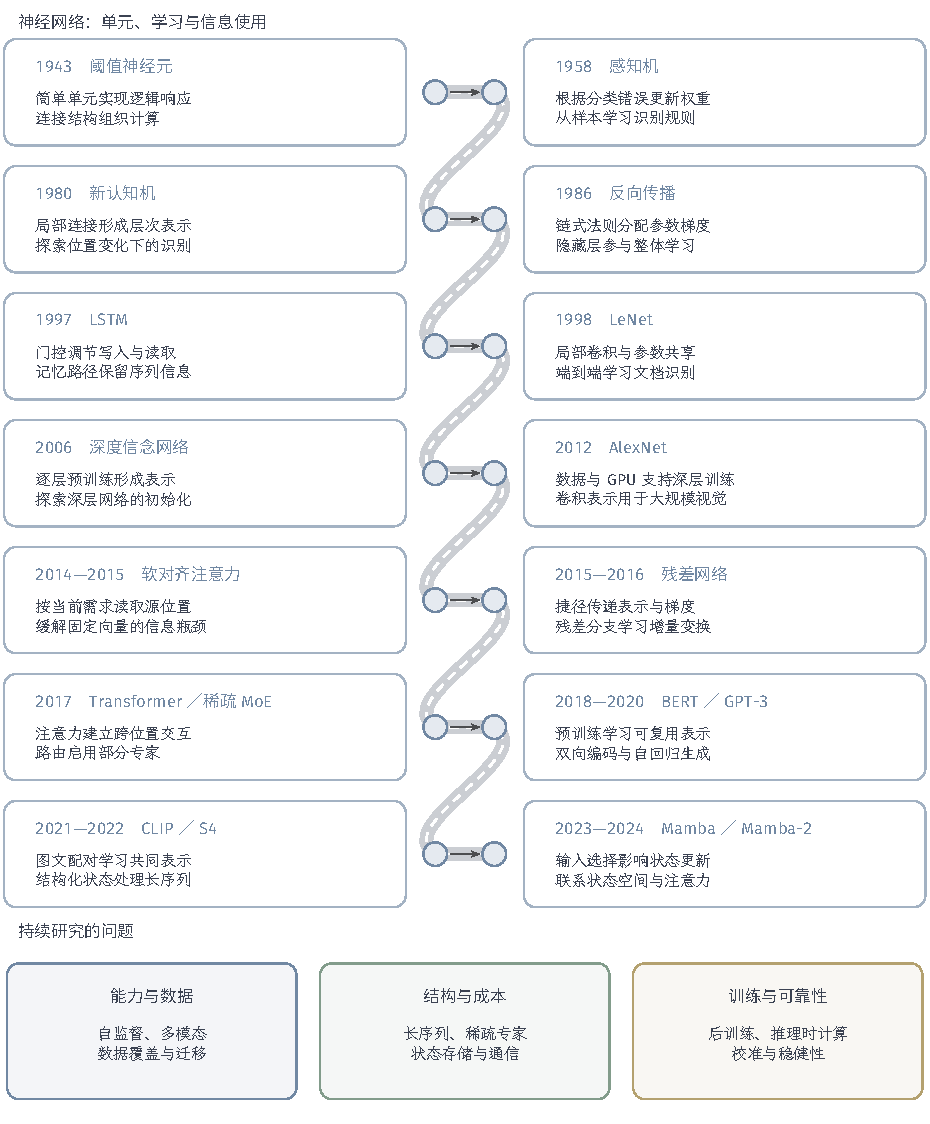
\includegraphics[width=157.406mm,height=.82\textheight,keepaspectratio]{figures/03-models/02-neural-network-models/tikz/neural-network-history/figure.pdf}
  \caption{神经网络的代表性发展节点。单元与连接决定可表达的计算，参数学习决定怎样获得表示，数据与计算条件决定可实现的规模；注意力、路由和状态更新进一步改变运行时的信息使用方式。日期对应代表论文的首次公开或发表时间，节点间距不按时间比例绘制。底部是持续研究的问题，不表示已经解决的终点。}
  \label{fig:neural-network-history}
\end{figure*}
\FloatBarrier

\section{本章小结}
\label{sec:neural-overview-summary}

神经网络把特征构造纳入可学习的计算路径。异或例子说明，原始坐标中的线性限制可以通过非线性中间表示改变，输出端仍可使用简单规则。多个单元共同编码信息、多个层继续组合表示，为这种变换提供了两种互补的组织方式。表示是否适合任务，则由输入信息、结构假设、学习目标与算法共同决定。

生物启发把多输入整合、局部回路和经验引起的连接变化带入人工模型。视觉感受野提示局部检测与层次组合，腹侧和背侧通路则说明不同任务需要保留不同信息。这种启发并未确定人工模型应复现多少生物细节：任务预测需要评价输出，生物解释需要对应观察，能效比较还要计入时间、通信与系统范围。

从阈值单元到现代架构，隐藏层扩大了可选函数的范围，反向传播把最终损失与内部参数相连，结构组织信息交互，数据和实现支持训练。表达能力、参数能否学得以及新样本上的表现因此成为三个相连但各有条件的问题。网络的名称或规模，不能代替对这三个问题的分析。

连接组织、信息交互与编码方式提供了比较后续架构的共同依据。局部共享、状态递推、关系聚合、内容读取和脉冲事件可以分别使用，也可以组合；其取舍由任务需要保留的信息、训练条件与计算资源决定。

\paragraph{扩展阅读}
Goodfellow等的《深度学习》从表示、优化与统计学习建立共同框架，Bishop与Bishop的教材进一步联系现代网络结构。各历史节点的原论文分别记录了结构贡献、训练条件与当时的任务设置，可与本章的机制比较对应\scite{goodfellow2016,bishop2024deep}

\chapter{前馈神经网络}
\label{chap:feedforward-networks}

第~\ref{chap:neural-network-overview}章用异或说明了隐藏表示的作用：两个非线性单元就能把原始坐标中无法线性分开的样本变成可分的表示。但那组权重是手工给出的。面对真实数据，网络应当怎样组织这些单元，训练目标怎样决定各层参数的变化，又凭什么相信训练结果可以用于未见样本？计算结构决定哪些输入可以组合，参数学习决定怎样从样本获得权重，预测能力还取决于训练结果在新样本上的风险。层数和训练误差只描述其中一部分。

本章以层状、全连接的前馈网络为主要对象，把前章的函数复合落实为可计算、可求导的模型。网络结构规定候选函数及其输出含义，参数学习把最终损失对各层参数的影响算出来，理论分析则区分表达一个函数与从有限数据学得低风险预测规则。常见应用把这些要素接回完整的输入、训练和预测过程。计算与求导沿用前文的向量、矩阵、损失和梯度。复杂度与稳定性用于把有限样本上的结果联系到新样本风险（相关分析参考\BookChapterRef{chap:deep-learning-theory}{第二卷“基础、理论和可信性”的“深度学习的可学习性”章}）。

\section{网络结构}
\label{sec:ffn-structure}

前馈性质规定的是计算依赖的方向：同一次前向计算中，后续结果不会沿有向环返回上游。具体连接范围和层宽可以另行选择。本节采用全连接的逐层结构，把一次预测展开为加权组合、非线性响应和任务输出三个环节。

\subsection{神经元}
\label{sec:ffn-neuron}

要把一组输入变成新的特征，可以让一个人工神经元读取若干数值，计算加权和，再通过激活函数得到输出。设单元的输入为$\bm{u}\in\mathbb{R}^{m}$，权重为$\bm{w}\in\mathbb{R}^{m}$，偏置为$b\in\mathbb{R}$，则
\begin{equation}
  z=\bm{w}^{\top}\bm{u}+b,
  \qquad h=\sigma(z)\text{。}
  \label{eq:ffn-unit}
\end{equation}
权重决定各个输入怎样共同影响单元，偏置改变单元响应的位置。这里的$z$称为\term{预激活值}（pre-activation），即非线性变换之前的加权结果；$h$是单元输出。没有偏置时，ReLU单元的分界$\bm{w}^{\top}\bm{u}=0$必须经过原点，加入偏置后便能移动这条分界。

同一层的多个单元可以各自读取整组输入，用不同权重计算不同坐标。这种\term{全连接层}（fully connected layer）让下一层每个单元与上一层每个单元相连。把一个单元的权重按行放入矩阵，就能用一次矩阵运算计算整层。沿用前章的列向量约定，设网络有$L$个隐藏层，输入为$\bm{x}\in\mathbb{R}^{d}$，令$d_0=d$、$\bm{h}^{(0)}=\bm{x}$，各隐藏层依次计算
\begin{equation}
  \begin{aligned}
    \bm{z}^{(\ell)}
      &=\bm{W}_\ell\bm{h}^{(\ell-1)}+\bm{b}_\ell,\\
    \bm{h}^{(\ell)}&=\sigma_\ell\!\left(\bm{z}^{(\ell)}\right),
    \qquad \ell=1,\ldots,L\text{。}
  \end{aligned}
  \label{eq:ffn-hidden-layers}
\end{equation}
其中$\bm{W}_\ell\in\mathbb{R}^{d_\ell\times d_{\ell-1}}$、$\bm{b}_\ell\in\mathbb{R}^{d_\ell}$，$\bm{z}^{(\ell)}$和$\bm{h}^{(\ell)}$都属于$\mathbb{R}^{d_\ell}$，$\sigma_\ell$逐坐标作用。上标$\ell$表示层的位置，不是幂，也不是参数更新的迭代步。

隐藏层之后还需一个与任务相配的输出层。记原始输出为$\bm{a}\in\mathbb{R}^{q}$、$d_{L+1}=q$，完整模型写为
\begin{equation}
  \begin{aligned}
    \bm{a}&=\bm{W}_{L+1}\bm{h}^{(L)}+\bm{b}_{L+1},\\
    \widehat{\bm{y}}&=g(\bm{a})\text{。}
  \end{aligned}
  \label{eq:ffn-output-map}
\end{equation}
矩阵$\bm{W}_{L+1}\in\mathbb{R}^{q\times d_L}$和向量$\bm{b}_{L+1}\in\mathbb{R}^{q}$参与学习，输出变换$g$由任务决定。$g$可以是恒等映射，也可以把得分转换为概率。用$\bm{\theta}\in\mathbb{R}^{p}$收集全部权重与偏置，模型记为$\bm{f}_{\bm{\theta}}(\bm{x})=\widehat{\bm{y}}$；标量输出时写$f_{\bm{\theta}}$。

图~\ref{fig:ffn-architecture}展示了这种分层依赖。输入层只提供数据，不计算一组新的可学习参数；隐藏层的每个坐标都是一次式\eqref{eq:ffn-unit}的计算。这就是前章引入的多层感知机：具有一个或多个全连接隐藏层、用非线性变换构造表示的前馈网络。这里的MLP采用可供梯度计算的非线性激活，区别于早期感知机作硬判定的阈值响应。

\begin{figure*}[htb]
  \centering
  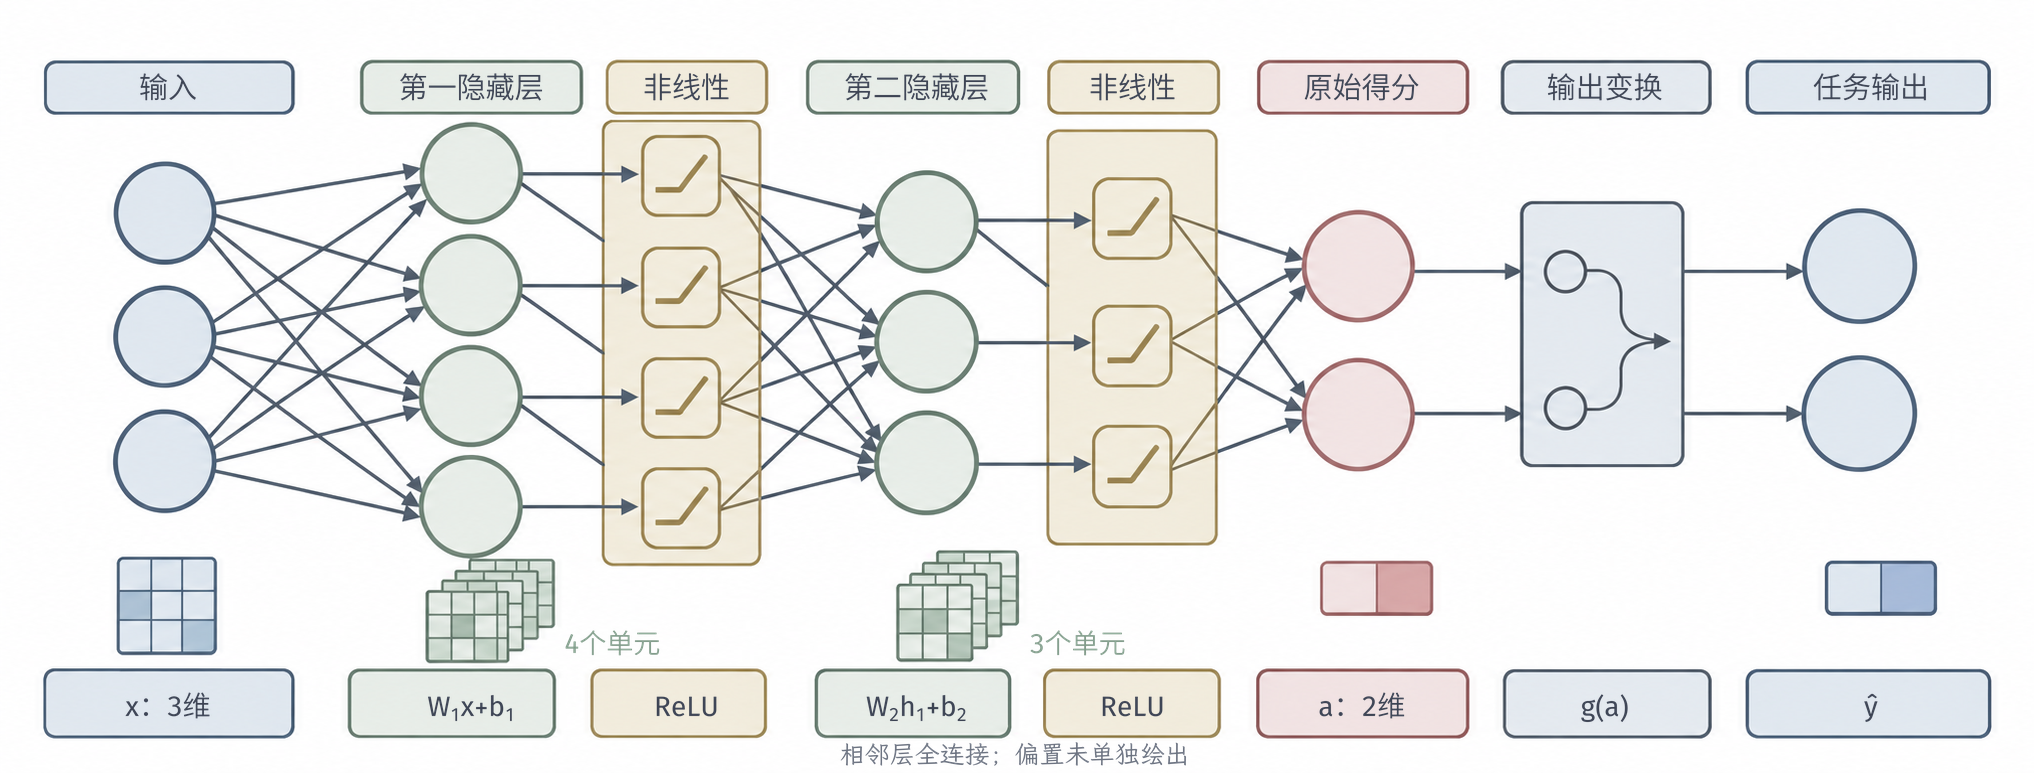
\includegraphics[width=169.000mm]{figures/03-models/02-neural-network-models/generated/ffn-architecture/figure.png}
  \caption{两个隐藏层的全连接前馈网络。左侧单元提供输入$\bm{x}$，中间两层计算隐藏表示，右侧单元产生原始得分$\bm{a}$，之后再使用任务规定的输出变换$g$。细线表示可学习的连接，层间箭头标明前向计算方向；每个目标单元还具有一个未画出的偏置。图中层宽依次为$3,4,3,2$，只是结构示例。}
  \label{fig:ffn-architecture}
\end{figure*}

对没有参数共享的上述网络，参数总数为
\begin{equation}
  p=\sum_{\ell=1}^{L+1}d_\ell(d_{\ell-1}+1)\text{。}
  \label{eq:ffn-parameter-count}
\end{equation}
括号内的两项分别来自每个单元的输入权重和偏置。若输入维度为$100$，两个隐藏层宽度均为$64$，输出维度为$1$，参数量为$64\times101+64\times65+65=10689$。这说明输入编码和层宽会直接改变模型规模。忽略激活和偏置的较小开销，一次单样本前向计算的乘加量与$\sum_\ell d_\ell d_{\ell-1}$同阶。这一计数衡量存储与运算规模；同样数量的参数能表达哪些关系，还由连接与激活决定，预测可靠性还需要样本与训练依据。

本文把$L$称为隐藏层数，把$d_\ell$称为第$\ell$层宽度。文献中的\term{深度}（depth）有时包含输出层，有时只计隐藏层，两种计数相差一个输出层，因此深度比较需要采用同一口径。跨层连接只要不构成有向环，也可以保持前馈性质；本章的逐层推导采用普通串联结构。

\subsection{激活函数}
\label{sec:ffn-activations}

前章已经证明，连续叠加仿射层仍然只是一次仿射变换。隐藏层需要非线性激活，使不同输入范围可以有不同响应。但非线性也会改变导数：有些函数把大幅输入变化压成很小的输出变化，有些函数把一部分输入直接置零，还有些函数让响应形状参与学习。这些响应方式分别改变可表达的关系、反传梯度和输出范围，也需要不同的数值运算。

本节按响应方式介绍常见函数：恒等与阶跃作为基准，双侧饱和函数限制输出范围，整流与指数型函数保留较大的正响应，自门控函数平滑地调节输入，Maxout与Softmax则联合处理多个预激活值。带参数函数的曲线随参数改变，图中的参数值因此构成比较条件；随机函数在训练与预测阶段采用的响应规则也可能不同。除特别说明外，输入记为标量$z$，输出记为$\sigma(z)$。

\subsubsection{恒等与阶跃}
\label{sec:ffn-activation-baselines}

若需要保留任意实数输出，可以使用\term{恒等函数}（identity function）；若只需要一个硬的二值判定，可以使用\term{阶跃函数}（step function）。两者分别为
\begin{equation}
  \operatorname{Identity}(z)=z,
  \qquad
  H(z)=\begin{cases}0,&z<0,\\1,&z\geq0\text{。}\end{cases}
  \label{eq:ffn-identity-step}
\end{equation}
恒等函数的导数为$1$，常用于回归输出或无需额外激活的投影；全部隐藏层都用恒等函数时，多层串联仍是仿射映射。阶跃函数适合表达阈值决策，但除阈值处不可微之外，在其余位置导数都为$0$，普通反向传播无法据此学习阈值单元的输入参数。预测时作硬判定与训练时使用连续可导替代，是两种不同用途。

\begin{figure*}[htb]
  \centering
  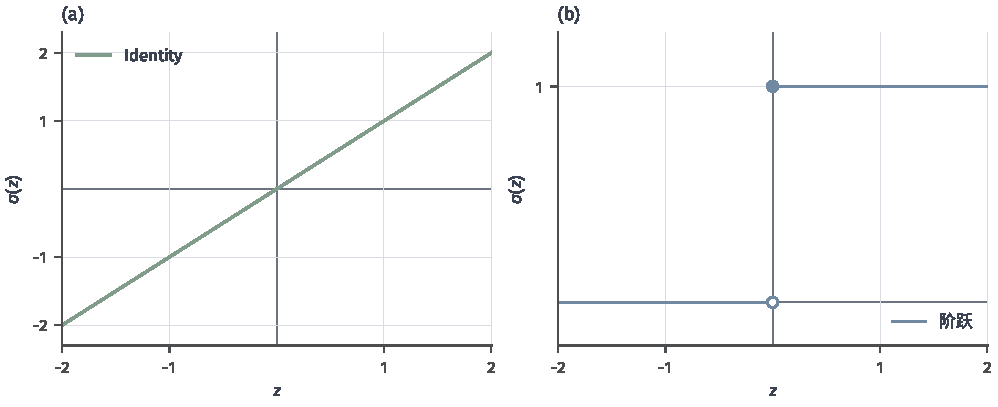
\includegraphics[width=159.059mm]{figures/03-models/02-neural-network-models/matplotlib/ffn-activation-basics/figure.pdf}
  \caption{恒等函数与阶跃函数的比较。左图保留输入，斜率恒为$1$；右图按零阈值输出$0$或$1$，空心点和实心点区分$z=0$两侧的端点约定。横轴为预激活值$z$，纵轴为输出；阶跃图中的跳跃不能通过普通局部导数传递学习信号。}
  \label{fig:ffn-activation-basics}
\end{figure*}

\subsubsection{双侧饱和函数}
\label{sec:ffn-activation-saturating}

当一个单元需要产生概率、控制系数或有界状态时，把任意实数压到有限区间是直接的选择。\term{Logistic函数}产生$(0,1)$内的响应，实践中常直接称为Sigmoid；\term{双曲正切函数}（hyperbolic tangent, Tanh）产生$(-1,1)$内的响应。Sigmoid也可泛指具有S形曲线的一类函数，这里用$s$专门表示Logistic函数：
\begin{equation}
  \begin{aligned}
    s(z)&=\frac{1}{1+\exp(-z)},
    &s'(z)&=s(z)(1-s(z)),\\
    \tanh(z)&=\frac{\exp(z)-\exp(-z)}{\exp(z)+\exp(-z)},
    &\tanh'(z)&=1-\tanh^2(z)\text{。}
  \end{aligned}
  \label{eq:ffn-saturating-activations}
\end{equation}
当$|z|$很大时，输出接近两端的极限，导数趋近于零。这种\term{饱和}（saturation）意味着输入继续变化，输出却几乎不变。Sigmoid导数至多为$1/4$；Tanh在原点的导数为$1$，并满足$\tanh(z)=2s(2z)-1$。Tanh关于原点对称，可以产生正负响应，但只有对称输入分布等条件才能进一步推出输出均值为零。

Sigmoid适合二分类概率、多标签概率和取值在$(0,1)$的控制门。当损失与事件标签构成概率模型时，这一响应才作为相应事件的概率；用在隐藏层时，它只是有界特征值。Tanh适合需要正负有界状态的模块，例如后续循环网络中的候选状态。两者用于许多层连续串联时，饱和区的小导数可能参与梯度衰减；传播中的权重矩阵同时可以放大或缩小信号，完整梯度尺度由沿途的两种作用共同决定。

若希望避免指数运算，可以用分段线性函数近似上述有界响应。\term{硬Sigmoid}（hard sigmoid，也称Hard-Logistic）和\term{硬Tanh}（hard tanh）将线性段之外的值截到边界：
\begin{equation}
  \begin{aligned}
    \operatorname{HardSigmoid}(z)
      &=\min\{1,\max\{0,\tfrac14z+\tfrac12\}\},\\
    \operatorname{HardTanh}(z)&=\min\{1,\max\{-1,z\}\}\text{。}
  \end{aligned}
  \label{eq:ffn-hard-saturating-activations}
\end{equation}
本节的HardSigmoid在$(-2,2)$内斜率为$1/4$，区间外为$0$；HardTanh在$(-1,1)$内斜率为$1$，区间外为$0$，其负端输出是$-1$。分段边界处的导数需要约定。HardSigmoid的线性段并没有唯一标准，一些实现采用$z/6+1/2$并在$\pm3$处截断；不同斜率与截断点会改变响应及导数，移植模型需要采用与原实现相同的定义\scite{pytorchHardsigmoid}

两种硬近似可用于受计算资源限制的门控或范围约束，代价是拐点不可微，截断区内还会出现严格为零的梯度。\term{Softsign函数}提供另一种有界响应，用绝对值而非指数控制幅度：
\begin{equation}
  \operatorname{Softsign}(z)=\frac{z}{1+|z|},
  \qquad
  \operatorname{Softsign}'(z)=\frac{1}{(1+|z|)^2}\text{。}
  \label{eq:ffn-softsign}
\end{equation}
它的值域也是$(-1,1)$，一阶导数连续，尾部导数以多项式速度趋零。它可用于需要有界正负响应的隐藏层或状态映射；与Tanh相比，它的尾部导数衰减更慢，具体输入处的梯度大小仍由各自导数值决定。

\begin{figure*}[htb]
  \centering
  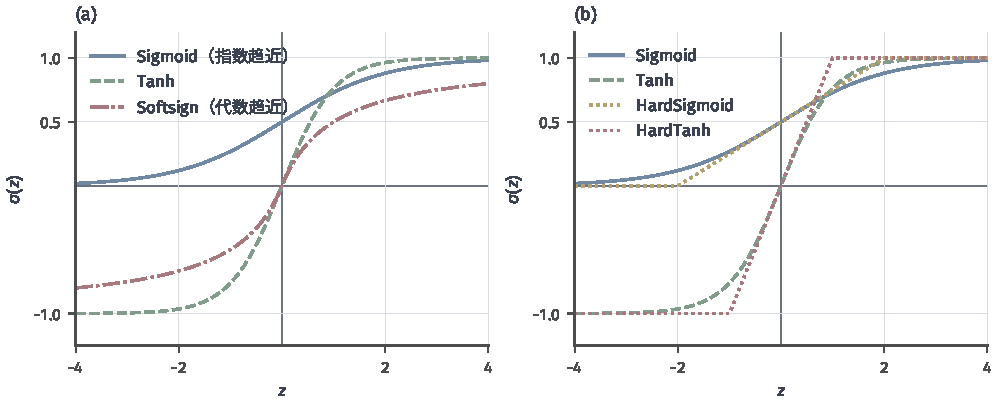
\includegraphics[width=159.059mm]{figures/03-models/02-neural-network-models/matplotlib/ffn-activations/figure.pdf}
  \caption{双侧饱和激活函数。左图比较Logistic／Sigmoid、Tanh与Softsign；Softsign采用长虚线，以便在黑白打印中仍能与Sigmoid区分，图例同时指出前者按代数速度、后者按指数速度趋近渐近值。右图将HardSigmoid和HardTanh与对应平滑函数比较。HardSigmoid采用式\eqref{eq:ffn-hard-saturating-activations}中的斜率$1/4$及截断点$\pm2$。}
  \label{fig:ffn-activations}
\end{figure*}

\subsubsection{整流函数及其变体}
\label{sec:ffn-activation-rectifiers}

ReLU采用前章的$\rho(z)=\max\{0,z\}$，正半轴斜率为$1$，负半轴输出和导数都为$0$。它只需比较与取值，能够产生严格为零的激活，可作为全连接或卷积隐藏层的基础选择。如果某单元对所有训练样本都长期落在负半轴，其输入权重可能难以得到数据梯度。失活对应当前参数和数据共同产生的负预激活；较深层的上游表示若随后改变，单元也可能重新进入正半轴。

让负半轴保留非零斜率，可以避免该区域完全阻断局部梯度。\term{带泄漏的ReLU}（leaky ReLU）使用固定$0<\alpha<1$，\term{参数化ReLU}（parametric ReLU, PReLU）则把负半轴斜率作为待学习参数：
\begin{equation}
  \begin{aligned}
    \operatorname{LeakyReLU}(z)
      &=\max\{0,z\}+\alpha\min\{0,z\},\\
    \operatorname{PReLU}_j(z)
      &=\max\{0,z\}+\alpha_j\min\{0,z\}\text{。}
  \end{aligned}
  \label{eq:ffn-leaky-prelu}
\end{equation}
PReLU的$\alpha_j$可以按单元、通道设置，也可以在一层内共享；若不另加约束，它并不天然位于$(0,1)$。给定上游梯度，斜率参数的局部求导规则是$\partial\operatorname{PReLU}_j(z)/\partial\alpha_j=\min\{0,z\}$，共享斜率时要累加各使用位置的贡献。PReLU增加的参数量取决于共享方式，通常每个单元、通道或层只增加一个斜率参数\scite{he2015rectifiers}

Leaky ReLU适合希望保留负响应且不增加待学习参数的隐藏层，PReLU适合允许数据调整负响应强度的模块。\term{随机化带泄漏ReLU}（randomized leaky ReLU, RReLU）沿用同一分段形式，但训练时从预先规定的区间$[l,u]$均匀采样负斜率$\alpha$，其中$0<l<u<1$，预测时通常采用$(l+u)/2$。每次采样产生一条不同曲线，使同一负输入在训练中受到不同缩放。预测采用确定斜率；这种训练扰动对误差的作用需要在相应任务上评价\scite{xu2015rectified}

如果部署还要求限制正响应，可以使用\term{ReLU6函数}，即
\begin{equation}
  \operatorname{ReLU6}(z)=\min\{6,\max\{0,z\}\}\text{。}
  \label{eq:ffn-relu6}
\end{equation}
它在$(0,6)$内保留斜率$1$，在两侧导数为$0$，常与移动端模型及有限数值范围的设计联系在一起。MobileNetV2使用了这类有界整流响应，但其线性瓶颈层还刻意省略非线性，说明激活要按层的职责选择\scite{sandler2018mobilenetv2}相对于ReLU，新增上界让较大的正输入也进入零导数区，有限范围与梯度传递因此形成取舍。

\begin{figure*}[htb]
  \centering
  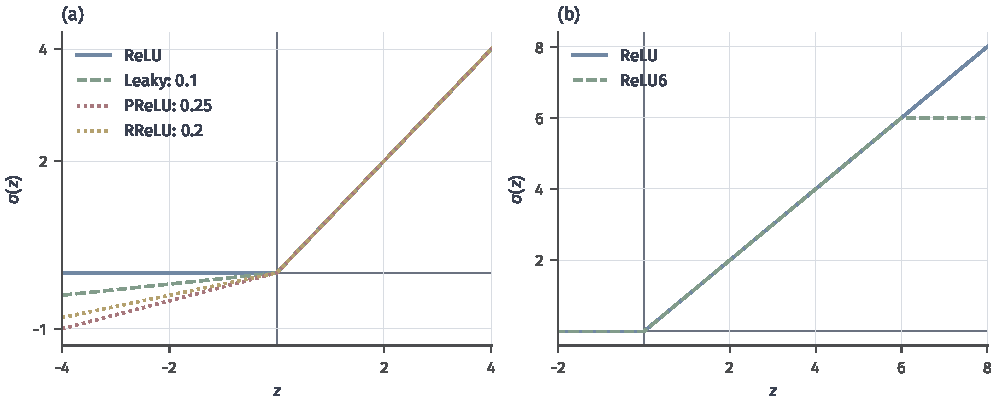
\includegraphics[width=159.059mm]{figures/03-models/02-neural-network-models/matplotlib/ffn-activation-rectifiers/figure.pdf}
  \caption{整流函数与负斜率变体。左图固定Leaky ReLU的$\alpha=0.1$、PReLU的$\alpha_j=0.25$，并以$\alpha=0.2$画出RReLU训练阶段的一种可能曲线；三者的形状差异来自斜率选择，PReLU与RReLU的区别主要在参数取得方式。右图比较ReLU与ReLU6，展示$z>6$时的截断。两图横轴范围不同。}
  \label{fig:ffn-activation-rectifiers}
\end{figure*}

有界函数与整流函数的差异集中在表~\ref{tab:ffn-activation-bounded}中。Sigmoid、Tanh和Softsign限制两端幅度，ReLU只截断负半轴，ReLU6还限制正端；这种范围差异会直接改变哪些输入能够传递梯度。

\begin{table*}[htb]
  \centering
  \small
  \begin{tabularx}{\linewidth}{@{}l l X X@{}}
    \toprule
    函数 & 输出范围 & 导数与参数特点 & 适用场景及主要边界 \\
    \midrule
    Identity & $\mathbb{R}$ & 导数为$1$ & 回归输出、线性投影；不增加非线性 \\
    阶跃 & $\{0,1\}$ & 非阈值处导数为$0$ & 硬判定；不能直接靠普通反向传播训练 \\
    Sigmoid & $(0,1)$ & 两端导数趋零 & 二分类、多标签、控制门 \\
    Tanh & $(-1,1)$ & 两端导数趋零 & 有界正负状态；深层饱和需关注 \\
    HardSigmoid & $[0,1]$ & 截断区导数为$0$ & 简单门控；需核对斜率与截断点 \\
    HardTanh & $[-1,1]$ & 截断区导数为$0$ & 有界状态；拐点与严格零梯度 \\
    Softsign & $(-1,1)$ & 一阶连续，尾部导数趋零 & 有界正负表示；尾部衰减方式不同 \\
    ReLU & $[0,+\infty)$ & 负半轴为$0$，正半轴为$1$ & 全连接、卷积隐藏层；可能失活 \\
    Leaky ReLU & $\mathbb{R}$ & 固定正负斜率 & 保留负梯度；斜率需设定 \\
    PReLU & 依赖$\alpha_j$ & 负斜率参与学习 & 学习响应形状；需说明参数共享方式 \\
    RReLU & $\mathbb{R}$ & 训练时随机负斜率 & 隐藏层训练扰动；预测规则不同 \\
    ReLU6 & $[0,6]$ & 两侧截断，中间斜率为$1$ & 有限范围、移动端；正端也会饱和 \\
    \bottomrule
  \end{tabularx}
  \caption{有界响应与整流激活的比较。Leaky ReLU和RReLU的范围按正负斜率均为正且非零书写；PReLU若不限制斜率，其输出范围随参数改变。所有分段函数都需在不可微边界约定求导规则。}
  \label{tab:ffn-activation-bounded}
\end{table*}

即使都用于限制输出幅度，求导行为也可能不同。Tanh和HardTanh都提供有界正负响应；按解析定义，前者在有限输入下保留非零导数，后者在截断区的导数严格为零。选择范围约束时，还需判断训练中的预激活值是否经常落到这些区域。

\subsubsection{指数型与平滑整流函数}
\label{sec:ffn-activation-exponential}

固定负斜率让负输出无限下降，另一种做法是使负响应逐渐接近一个有限下界。\term{指数线性单元}（exponential linear unit, ELU）在正半轴保留输入，在负半轴使用指数曲线：
\begin{equation}
  \operatorname{ELU}_{\alpha}(z)=
  \begin{cases}
    z,&z>0,\\
    \alpha(\exp(z)-1),&z\leq0,
  \end{cases}
  \qquad \alpha>0\text{。}
  \label{eq:ffn-elu}
\end{equation}
负半轴导数为$\alpha\exp(z)$，对有限负输入非零，但在$z\to-\infty$时趋零；输出趋近$-\alpha$。ELU连续，只有$\alpha=1$时左右一阶导数才在原点一致，但原点左右的二阶导数不同。ELU可用于希望保留负值并控制负端幅度的隐藏层；负响应允许层输出向两侧分布，实际均值仍由输入分布和权重决定\scite{clevert2016elu}

\term{缩放指数线性单元}（scaled exponential linear unit, SELU）进一步把ELU整体乘以固定系数：
\begin{equation}
  \operatorname{SELU}(z)=\kappa
  \begin{cases}
    z,&z>0,\\
    \alpha(\exp(z)-1),&z\leq0,
  \end{cases}
  \label{eq:ffn-selu}
\end{equation}
其中常用常数为$\alpha\approx1.6733$、$\kappa\approx1.0507$。它用于\term{自归一化网络}（self-normalizing neural network），即在规定假设下让层间激活的均值与方差趋向受控范围的前馈网络。相应分析依赖输入与权重的统计条件；常配合输入标准化、权重方差为$1/\mathrm{fan\text{-}in}$的初始化，以及为保持统计量设计的AlphaDropout。这里fan-in是一个单元的输入连接数，初始化的具体说明见第~\ref{sec:ffn-initialization}节。自归一化结论依赖这套激活、初始化与丢弃规则共同满足统计假设，替换其中一项也会改变分析条件\scite{klambauer2017selu}

如果目标是输出严格正值而又保持平滑，可以使用\term{Softplus函数}：
\begin{equation}
  \operatorname{Softplus}(z)=\log(1+\exp(z)),
  \qquad \operatorname{Softplus}'(z)=s(z)\text{。}
  \label{eq:ffn-softplus}
\end{equation}
它在正端接近$z$，在负端趋近$0$，但有限输入下输出严格大于$0$，不会产生ReLU式的精确零激活。Softplus可作为平滑隐藏激活，也适合将任意得分映射为正尺度、强度或方差参数；需要严格正下界时还可加上一个固定小常数。计算时使用$\max\{z,0\}+\log(1+\exp(-|z|))$可避免指数溢出。因此Softplus的用途由平滑性和正值约束决定；隐藏分类响应与正尺度输出采用它时，所要满足的条件不同。

\begin{figure}[htbp]
  \centering
  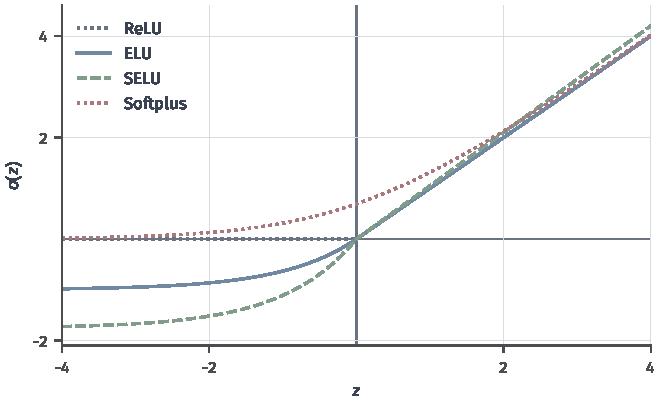
\includegraphics[width=105.412mm]{figures/03-models/02-neural-network-models/matplotlib/ffn-activation-exponential/figure.pdf}
  \caption{ELU、SELU与Softplus的响应。ELU使用$\alpha=1$，SELU使用式\eqref{eq:ffn-selu}中的常数，ReLU作为共同参照。ELU与SELU允许负输出并在负端趋向有限下界；Softplus始终为正，且平滑地趋近正半轴上的线性响应。}
  \label{fig:ffn-activation-exponential}
\end{figure}

\subsubsection{自门控函数}
\label{sec:ffn-activation-self-gated}

ReLU根据输入的正负作硬切换，也可以让输入乘一个连续变化的系数。\term{Swish函数}使用输入自身计算保留系数：
\begin{equation}
  \operatorname{Swish}_{\beta}(z)=z s(\beta z),
  \qquad \beta\geq0\text{。}
  \label{eq:ffn-swish}
\end{equation}
$\beta$可以固定，也可以参与学习。$\beta=0$时函数为$z/2$；$\beta=1$时得到\term{Sigmoid加权线性单元}（sigmoid-weighted linear unit, SiLU）；当$\beta\to+\infty$时，对每个固定输入趋向ReLU。这里的极限只描述固定输入处的响应值；不同$\beta$还会改变各输入处的导数，从而改变训练过程\scite{ramachandran2017swish}

计算输入敏感度及可学习门参数的梯度，需要分别对输入与门参数求导：
\begin{equation}
  \begin{aligned}
    \operatorname{Swish}_{\beta}'(z)
      &=s(\beta z)+\beta z s(\beta z)(1-s(\beta z)),\\
    \frac{\partial\operatorname{Swish}_{\beta}(z)}{\partial\beta}
      &=z^2s(\beta z)(1-s(\beta z))\text{。}
  \end{aligned}
  \label{eq:ffn-swish-derivatives}
\end{equation}
SiLU采用上述Swish族中固定门参数的实例。SiLU在强化学习函数逼近等场景中也有使用\scite{elfwing2018silu}SiLU可作为全连接、卷积或门控前馈模块中的平滑激活；在有限负区间内导数可能为负，负尾部导数又趋零。若学习$\beta$并要求保持非负，还需明确约束方式。

\begin{figure}[htbp]
  \centering
  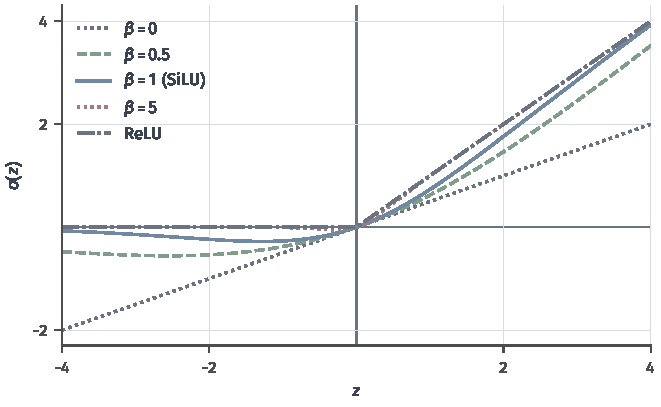
\includegraphics[width=105.412mm]{figures/03-models/02-neural-network-models/matplotlib/ffn-activation-swish/figure.pdf}
  \caption{Swish在不同$\beta$下的函数图像。$\beta=0$给出线性函数$z/2$，$\beta=1$就是SiLU，较大的$\beta$逐渐形成接近ReLU的响应。图中参数固定为$0,0.5,1,5$，ReLU用作极限参照；它不展示可学习$\beta$在某次训练中的实际轨迹。}
  \label{fig:ffn-activation-swish}
\end{figure}

\term{高斯误差线性单元}（Gaussian error linear unit, GELU）采用标准正态累积分布函数$\Phi$作为保留系数：
\begin{equation}
  \operatorname{GELU}(z)=z\Phi(z),
  \qquad \operatorname{GELU}'(z)=\Phi(z)+z\varphi(z)\text{。}
  \label{eq:ffn-smooth-gates}
\end{equation}
其中$\varphi(z)=\exp(-z^2/2)/\sqrt{2\pi}$是标准正态密度。GELU在全实数上平滑，但公式中的分布函数为每个输入确定一个保留系数，执行时采用确定响应。它常作为Transformer前馈模块的激活选择，平滑性保证局部导数连续，训练所得解的损失仍由完整目标与更新过程决定。常见近似为$z s(1.702z)$，或者
\begin{equation}
  \operatorname{GELU}(z)\approx
  \frac z2\left(1+\tanh\!\left[\sqrt{\frac2\pi}
  (z+0.044715z^3)\right]\right)\text{。}
  \label{eq:ffn-gelu-approximation}
\end{equation}
使用哪种近似会改变实际数值与导数，这会影响复现结果，因此模型记录需要标明精确式或近似式；GELU与SiLU的保留系数不同\scite{hendrycks2016gelu}

\term{Mish函数}进一步用Softplus和Tanh形成平滑的保留系数\scite{misra2019mish}其定义为
\begin{equation}
  \operatorname{Mish}(z)=z\tanh(\operatorname{Softplus}(z))\text{。}
  \label{eq:ffn-mish}
\end{equation}
令$t=\tanh(\operatorname{Softplus}(z))$，乘积与链式法则给出导数$t+zs(z)(1-t^2)$。Mish在负半轴保留一段负响应，负尾部趋近零，正端接近线性，可作为视觉网络或普通隐藏层的另一种平滑选择；原论文的比较是在指定模型与数据上进行的，这些设置决定了所报告收益的适用范围。

这些平滑函数需要指数、Tanh或正态分布函数计算。若希望用简单分段运算近似SiLU，可使用\term{硬Swish}（hard swish, Hardswish）。MobileNetV3在面向移动端的结构中使用这种响应\scite{howard2019mobilenetv3}其定义为
\begin{equation}
  \operatorname{Hardswish}(z)=z\frac{\operatorname{ReLU6}(z+3)}6
  =\begin{cases}
    0,&z\leq-3,\\
    z(z+3)/6,&-3<z<3,\\
    z,&z\geq3\text{。}
  \end{cases}
  \label{eq:ffn-hardswish}
\end{equation}
它在中间区间的导数为$(2z+3)/6$，在两端分别为$0$和$1$，在$\pm3$处不具有唯一导数。这里的门采用斜率$1/6$的硬Sigmoid形式，与前面斜率$1/4$的版本具有不同的线性段与截断点。实际速度取决于算子与硬件实现，而不只取决于公式中出现几个基本运算。

\begin{figure*}[htb]
  \centering
  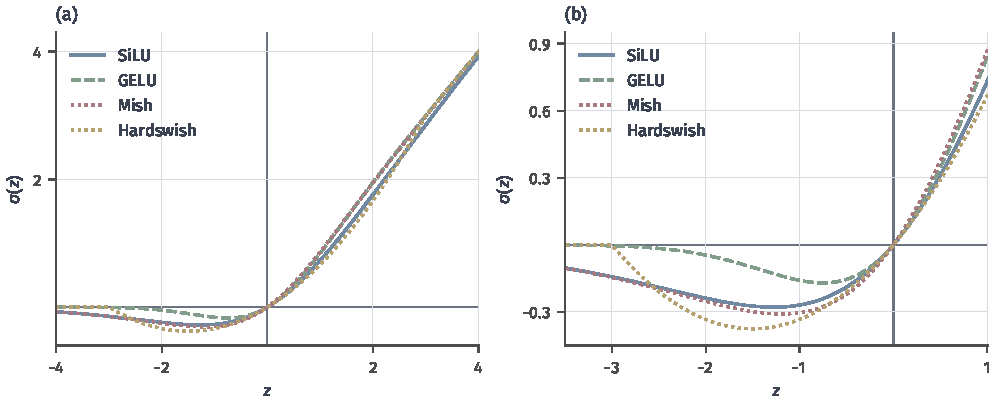
\includegraphics[width=159.059mm]{figures/03-models/02-neural-network-models/matplotlib/ffn-activation-smooth/figure.pdf}
  \caption{SiLU、GELU、Mish与Hardswish。左图展示整体响应，右图放大原点附近的负值和过渡区域；GELU按标准正态累积分布函数计算响应。它们在正端接近线性，但负区间的形状和拐点不同。SiLU、GELU与Mish平滑，Hardswish含有分段边界；两图使用不同坐标范围以显示细节。}
  \label{fig:ffn-activation-smooth}
\end{figure*}

\subsubsection{Maxout与Softmax}
\label{sec:ffn-activation-vector}

以上函数分别作用于一个标量。若希望一个单元从若干候选响应中选择最大者，可以使用\term{Maxout单元}（maxout unit）：它先计算$K$个仿射响应，再取最大值，响应的分段形状由权重学习得到。对于输入$\bm{u}\in\mathbb{R}^{m}$，其定义为
\begin{equation}
  z_k=\bm{w}_k^{\top}\bm{u}+b_k,
  \qquad h=\max_{1\leq k\leq K}z_k\text{，}
  \label{eq:ffn-maxout}
\end{equation}
其中每个$\bm{w}_k\in\mathbb{R}^{m}$、$b_k\in\mathbb{R}$都参与学习。只有一个严格最大响应时，梯度传给这一响应；多个响应并列最大时需约定分配方式。固定一个响应为零、另一个为$\bm{w}^{\top}\bm{u}+b$，就得到ReLU这一特殊形式。一个Maxout单元对输入表示为凸分段仿射函数；多层复合还包含可正可负的线性组合，完整网络的凸性须由整体计算判断\scite{goodfellow2013maxout}

Maxout适合希望学习分段响应形状的隐藏单元，也曾与Dropout联合研究。相对于一个普通仿射响应，它有$K$套权重与偏置，参数和响应计算量通常约增至$K$倍，这$K$套响应都要分别计算。梯度的截断由最大值选择决定：长期未被选中的分支可能收不到梯度。它还不再是式\eqref{eq:ffn-hidden-layers}中逐坐标作用于一个仿射响应的激活，反向计算需使用最大值选择对应的规则。

把$K$个得分转换为互斥事件的概率时，可以用\term{归一化指数映射}（softmax）让较大得分对应较大概率，并把概率总和固定为一。
对$\bm{z}\in\mathbb{R}^{K}$，其第$k$个输出为
\begin{equation}
  p_k=\operatorname{softmax}(\bm{z})_k
  =\frac{\exp(z_k)}{\sum_{j=1}^{K}\exp(z_j)},
  \qquad \sum_{k=1}^{K}p_k=1\text{。}
  \label{eq:ffn-softmax-activation}
\end{equation}
每个概率依赖全部输入坐标；画一维响应曲线时，需要固定其余坐标。
Jacobian矩阵描述每项概率对各得分的变化（公式参考\BookEquationRef{eq:analysis-softmax-jacobian}{第一卷“数学准备”的softmax求导公式}）。
Softmax适合互斥多分类输出和需要归一化权重的模块；多标签输出则通常分别使用Sigmoid。
训练时把Softmax与交叉熵合并，可以得到更直接且数值稳定的梯度，下一小节将展开。

\begin{figure*}[htb]
  \centering
  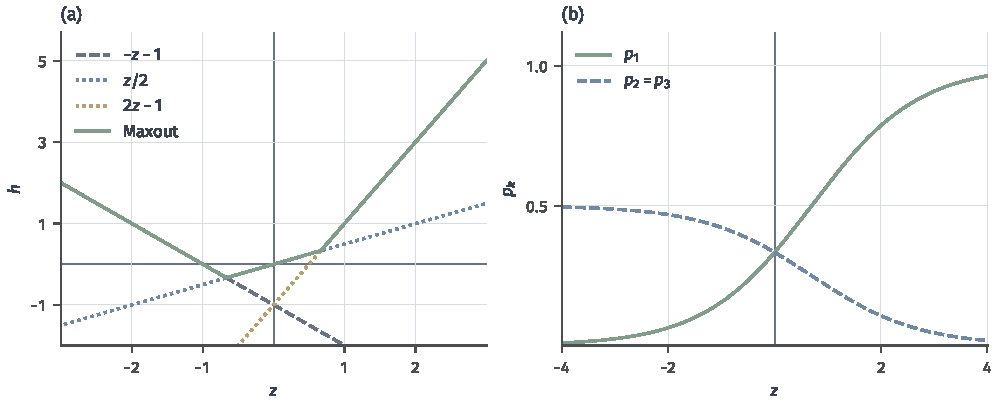
\includegraphics[width=159.059mm]{figures/03-models/02-neural-network-models/matplotlib/ffn-activation-vector/figure.pdf}
  \caption{Maxout和Softmax的一维观察方式。左图取三个仿射候选$-z-1$、$0.5z$和$2z-1$，粗实线是它们的最大值包络；它展示固定参数后沿一维输入的Maxout响应。右图固定三类得分为$(z,0,0)$，绘出三项Softmax概率，其中$p_2=p_3$，用同一条曲线标注。这些切片不能代表所有输入与参数下的唯一函数图像。}
  \label{fig:ffn-activation-vector}
\end{figure*}

\subsubsection{激活函数的比较与选择}
\label{sec:ffn-activation-selection}

表~\ref{tab:ffn-activation-bounded}归纳了前面的有界响应与整流函数，表~\ref{tab:ffn-activation-smooth}补充指数型、自门控与向量变换。两表中的输出范围对应该层的任务约束，导数特点说明哪些输入区间能传递学习信号，参数与随机机制则说明响应怎样取得。曲线比较只呈现固定参数下的形状，训练还包括参数更新或随机采样。



\begin{table*}[htb]
  \centering
  \small
  \begin{tabularx}{\linewidth}{@{}l l X X@{}}
    \toprule
    函数 & 输出范围 & 导数与参数特点 & 适用场景及主要边界 \\
    \midrule
    ELU & $(-\alpha,+\infty)$ & 负端导数趋零，$\alpha$固定 & 允许负响应；零均值没有无条件保证 \\
    SELU & $(-\kappa\alpha,+\infty)$ & 固定缩放与负指数响应 & 自归一化MLP；需配套统计条件 \\
    Softplus & $(0,+\infty)$ & 平滑，导数为Sigmoid & 正尺度输出、平滑隐藏层；无精确零 \\
    Swish／SiLU & 依赖$\beta$ & $\beta$固定或学习，SiLU取$1$ & 平滑隐藏层、前馈模块；局部可非单调 \\
    GELU & 有负下界，正端无界 & 平滑，精确式或近似式 & Transformer前馈模块；非随机采样 \\
    Mish & 有负下界，正端无界 & 平滑，复合运算 & 视觉或其他隐藏层；收益需验证 \\
    Hardswish & $[-3/8,+\infty)$ & 两个分段边界 & 移动端响应；速度取决于实现 \\
    Maxout & 依赖候选仿射响应 & 选中分支获梯度，$K$套参数 & 学习分段函数；分支可能少获梯度 \\
    Softmax & 概率单纯形内部 & 联合依赖全部得分 & 互斥类别、归一化权重；非逐坐标激活 \\
    \bottomrule
  \end{tabularx}
  \caption{指数型、自门控与向量变换的比较。Swish在$\beta=0$时是线性函数；其余正$\beta$情形具有有限负下界。Softmax按$K\geq2$书写，输出各项严格为正且总和为$1$。表中的平滑性描述固定参数的标量函数，不能替代整条计算路径的可微性检查。}
  \label{tab:ffn-activation-smooth}
\end{table*}

若该层预测概率或正尺度，输出约束通常决定选择：互斥类别用Softmax，多个可共存标签分别用Sigmoid，正尺度可以用Softplus。若该层构造隐藏表示，则需要比较非线性、活动范围与梯度。ReLU提供简单的分段响应，Leaky ReLU与PReLU保留负梯度，GELU与SiLU提供平滑过渡；SELU与特定初始化和统计条件配套，采用它时需要同时确定这些条件。

计算成本也必须放回实现环境。分段线性函数少用指数等运算，但向量化、融合算子和内存访问可能改变实际耗时。平滑函数可用于需要连续导数的模型，其导数仍可能在某些输入区间很小；增加可学习斜率也可能改变初始化时的合适尺度。比较预测性能时，应固定数据划分、结构和评价口径，并说明是否重新调节学习率与初始化，才能区分激活变化和配套设置变化的影响。

% 历史开篇的两条完整边注文献需要与段落一起容纳。
\Needspace{16\baselineskip}
\subsubsection{从阈值单元到平滑门控：发展脉络}
\label{sec:ffn-activation-history}

McCulloch与Pitts在1943年把神经活动的“全或无”性质写成阈值单元；Rosenblatt在1958年的感知机工作中进一步讨论了连接如何从样本中调整\scite{mcculloch1943,rosenblatt1958}这些早期模型用单元的开关组合表达判定。硬阈值便于表达逻辑关系，但其普通导数几乎处处为零，无法直接承担本章所用的多层梯度学习。

当隐藏层需要通过损失学习表示时，连续响应提供了可用的局部导数。Rumelhart、Hinton与Williams在1986年的反向传播论文中使用Logistic响应，展示了隐藏单元怎样随训练形成特征。这一工作将可微的连续响应与隐藏表示的学习结合起来，使激活函数的选择与训练机制紧密相连\scite{rumelhart1986}

Sigmoid与Tanh随后也暴露出深层训练的尺度问题：两端饱和时，导数会变小，Sigmoid在原点附近的输出又以二分之一为中心。2010年Glorot与Bengio的工作把激活响应与初始化放在一起分析，考察了单元可导之外的传播条件：活动值和梯度经过多层之后是否仍有合适尺度。Tanh把输出中心移到零附近，但仍保留两端饱和的边界\scite{glorot2010initialization}

这项工作的对照还表明，即使保留同一种激活，改变权重初始化方式也会改变各层活动值与梯度的尺度。选择激活函数时，因而还要把初始化和层深放在一起考察：一条曲线的局部斜率不足以描述整条网络的训练状态。第~\ref{sec:ffn-initialization}节将从信号的二阶矩出发解释这种配合，区分Tanh的中心响应与ReLU的半轴截断。

整流函数让设计重点转向稀疏响应和正半轴上的线性传播。Nair与Hinton在2010年研究了受限玻尔兹曼机中的整流单元；Glorot、Bordes与Bengio在2011年进一步比较深层前馈网络的整流与Tanh响应。这两项工作分别在生成模型与深层判别网络中展示了整流响应的作用。正半轴不饱和缓解了一类梯度衰减，负半轴的零导数又促使后续方法保留泄漏斜率或允许负响应\scite{nair2010rectifiers,glorot2011rectifiers}

较新的分支把注意力转向平滑过渡与输入相关的门控。2016年的GELU按输入幅度平滑加权；2017年的Swish工作通过函数搜索研究自门控响应，并与ReLU比较。两者都保留较大的正响应，同时用平滑过渡替代正负区域之间的硬切换\scite{hendrycks2016gelu,ramachandran2017swish}

本节介绍的带斜率变体、指数响应和硬近似，分别延伸了可学习形状、信号尺度与计算成本这些方向。历史上的改进解决的是特定结构和训练设置中的问题；这些设置也构成今天复用相应结果时的条件。Sigmoid和Softmax在概率输出中的用途，则由预测对象决定，并不因隐藏层采用ReLU或平滑门控而消失。

\subsection{输出和学习目标}
\label{sec:ffn-output-objectives}

隐藏层得到的是一组可供后续使用的数值，输出层则要回答任务中的具体问题：预测一个连续数值、判断一个事件是否成立、从多个类别中选一个，还是生成供其他模块使用的表示？这些问题对应不同的输出空间。选定输出变换$g$之后，还需用损失函数说明什么预测算好、错误怎样计分。下面始终把最后一层的原始得分记为$\bm{a}$，区分原始得分、预测结果与训练损失。

图~\ref{fig:ffn-output-heads}把五种任务放在同一个前馈结构之后比较：左侧逐层形成隐藏表示，右侧按任务选择一个输出头，即把隐藏表示转换成所需预测的最后一组计算。各头有各自的权重、偏置和训练目标；图中的分支表示可替换的方案，并不表示必须同时训练五个任务。

\begin{figure*}[!htb]
  \centering
  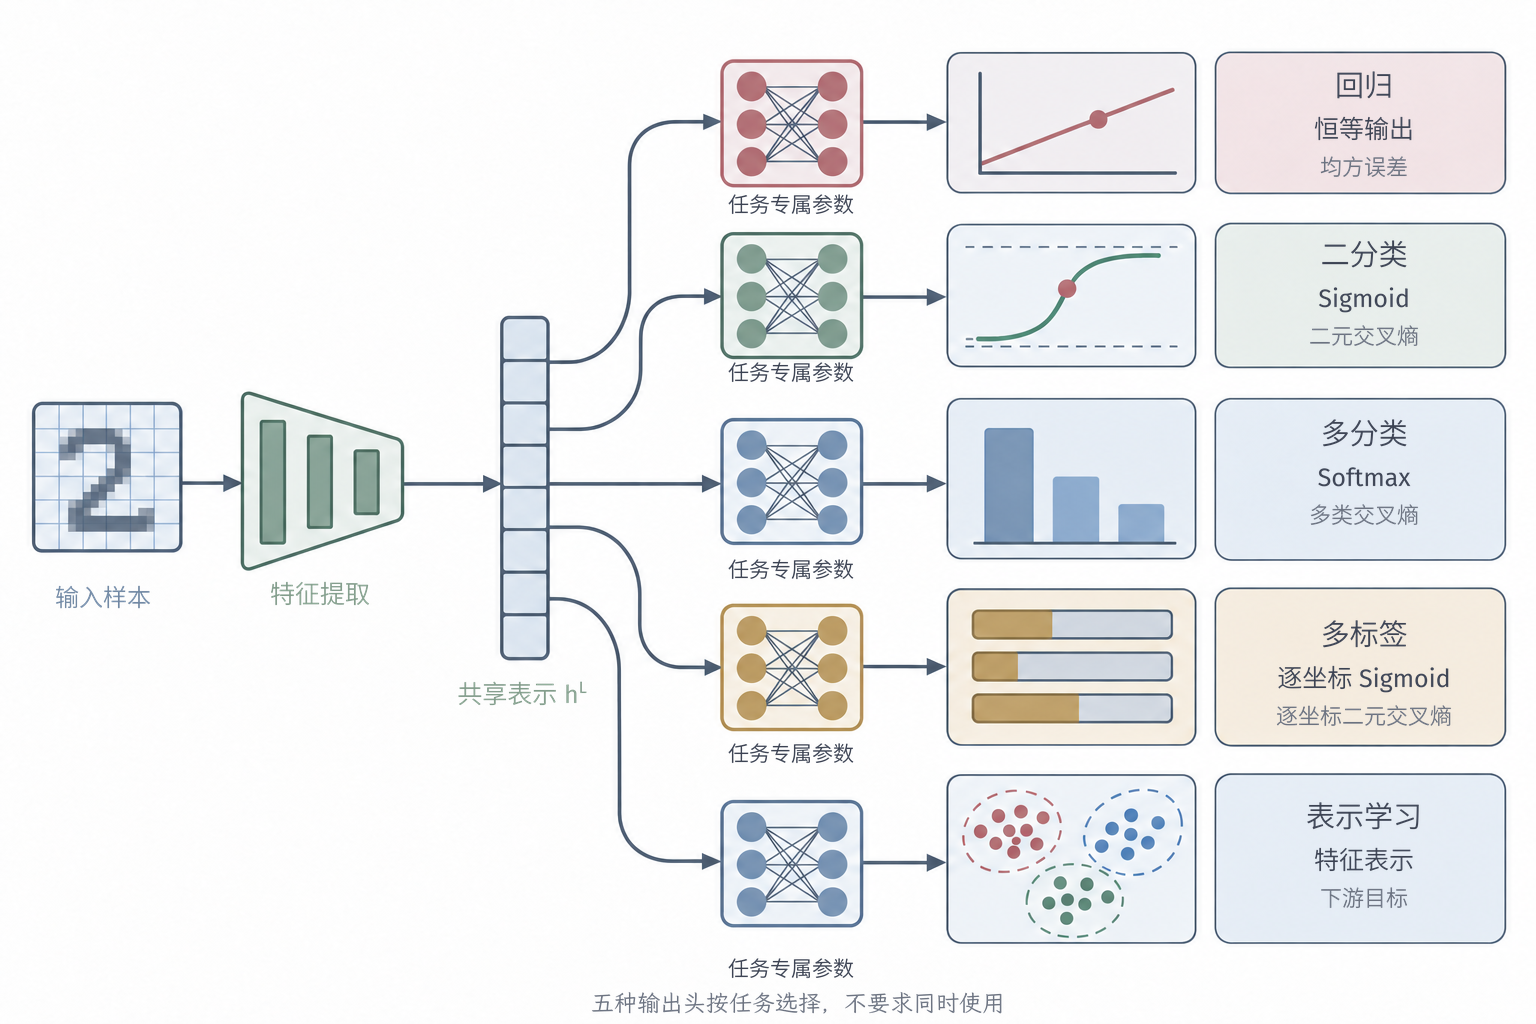
\includegraphics[width=130.048mm]{figures/03-models/02-neural-network-models/generated/ffn-output-heads/figure.png}
  \caption{共同的前馈结构与五种可替换的输出头。左侧输入单元经隐藏单元形成$\bm{h}^{(L)}$；汇合线传递整组隐藏坐标，不执行求和。右侧单元产生各任务自己的原始得分，每个单元都读取全部隐藏坐标，并具有独立的输出权重与偏置。回归与二分类头只需一个得分；多类分类头联合归一化，多标签分类头逐坐标变换；表示头产生由下游任务约束的表示。向量头仅画三个坐标示意，实际维度由任务决定。右侧文字区分预测量与训练目标，隐藏激活无需与输出变换相同。}
  \label{fig:ffn-output-heads}
\end{figure*}

\subsubsection{回归：预测连续数值}
\label{sec:ffn-output-regression}

回归的目标是连续数值，例如经过单位缩放的房价。对标量目标$y\in\mathbb{R}$，令$q=1$，输出层只产生一个得分$a$；采用恒等变换$g(a)=a$时，预测值就是$\widehat y=a$。平方损失衡量预测值与目标的距离：
\begin{equation}
  \ell(a,y)=\frac12(a-y)^2,
  \qquad \frac{\partial\ell}{\partial a}=a-y\text{。}
  \label{eq:ffn-regression-loss}
\end{equation}
系数$1/2$用于简化导数，不改变仅有这一损失时的最优预测。若教学样本的目标为$2.5$、当前预测为$2$，损失为$0.125$，对输出的导数为$-0.5$；沿负梯度方向调整输出，会让它增大并接近目标。多个连续目标可以使用向量输出，以及$\frac12\lVert\bm{a}-\bm{y}\rVert_2^2$；不同坐标的单位与尺度需要在数据处理或损失权重中考虑。

平方损失还规定了预测的统计含义。在二阶矩有限、可选函数足够自由时，使条件期望损失最小的预测是$\mathbb{E}[y\mid\bm{x}]$，即给定输入后的条件均值。因而同一个输入对应多种可能结果时，平方损失倾向于预测它们的均值，并不直接输出所有可能结果。

输出范围应与目标配合。若预测正尺度，可以令$\widehat y=\operatorname{Softplus}(a)$，再对$\widehat y$计算损失；此时对$a$求导还需乘输出变换的导数。若同时预测不确定性，可以让网络输出均值和正方差，再用所选概率分布的负对数似然训练。约束预测值的范围与建立一个完整的条件分布，是两个不同的设计决定。

\subsubsection{二分类：预测一个正类概率}
\label{sec:ffn-output-binary}

二分类判断一个事件是否成立，例如一封邮件是否属于垃圾邮件。令$y\in\{0,1\}$，其中$1$表示正类。输出层仍只需要一个实数$a$，经过Sigmoid得到
\[
  p=s(a),\qquad P_{\bm{\theta}}(y=1\mid\bm{x})=p,
  \qquad P_{\bm{\theta}}(y=0\mid\bm{x})=1-p\text{。}
\]
这里$p$是模型给出的正类概率，$a$称为\term{logit}，即对数几率$\log(p/(1-p))$。两个类别的概率已经由$p$和$1-p$共同确定，无须再设置两个彼此独立的概率输出。

在这个伯努利模型下，正确标签的概率为$p^y(1-p)^{1-y}$。对它取负对数，就得到二元交叉熵：
\begin{equation}
  \begin{aligned}
    \ell(a,y)
      &=-y\log p-(1-y)\log(1-p)\\
      &=\log(1+\exp(a))-ya\text{。}
  \end{aligned}
  \label{eq:ffn-binary-cross-entropy}
\end{equation}
若$y=1$而$p=0.8$，损失约为$0.2231$；若把这个正例的概率降到$0.2$，损失会增至约$1.6094$。交叉熵不仅考察最后选对哪一类，还区分模型给正确标签分配了多少概率。

式\eqref{eq:ffn-binary-cross-entropy}以原始得分$a$为输入，把Sigmoid和损失合在一起计算。其稳定形式为$\max\{a,0\}-ya+\log(1+\exp(-|a|))$，导数为$\partial\ell/\partial a=p-y$。这避免了先得到极接近$0$或$1$的概率再取对数。预测类别时还需选定阈值$\tau$，例如按$p\geq\tau$判为正类；误判代价或业务约束不同，所需阈值也可能不同。硬判定用于决策，连续概率与损失用于学习。

图~\ref{fig:ffn-output-heads}的回归与二分类分支共用同一种隐藏结构。两者都可以只产生一个原始得分，差别发生在输出解释和学习目标；二分类的概率变换不会要求隐藏层也使用Sigmoid。


\subsubsection{互斥多分类：预测一个类别}
\label{sec:ffn-output-multiclass}

若一个样本恰好属于$K$个类别中的一个，例如一张数字图像对应一个数字类别，需要输出一组相互竞争的概率。设$y\in\{1,\ldots,K\}$、$q=K$，输出层的每个坐标$a_k$是对应类别的原始得分。Softmax将整组得分转换为概率：
\begin{equation}
  p_k=\frac{\exp(a_k)}{\sum_{j=1}^{K}\exp(a_j)},
  \qquad \sum_{k=1}^{K}p_k=1,\qquad
  \widehat y=\operatorname*{arg\,max}_{k}p_k\text{。}
  \label{eq:ffn-multiclass-output}
\end{equation}
最大概率并列时还需约定决策规则。与逐坐标使用Sigmoid相比，Softmax的分母让所有类别共同参与归一化：提高一个类别的概率，必然改变至少一个其他类别的概率。

正确标签的概率为$p_y$。多类交叉熵就是这个概率的负对数，把Softmax代入后可写成
\begin{equation}
  \ell(\bm{a},y)=-\log p_y
  =-a_y+\log\sum_{j=1}^{K}\exp(a_j)\text{。}
  \label{eq:ffn-multiclass-cross-entropy}
\end{equation}
对$a_k$求导得到$p_k-\mathbb{I}\{y=k\}$。例如教学样本有三类，$y=2$、$\bm{p}=(0.1,0.7,0.2)^{\top}$，则损失约为$0.3567$，得分梯度为$(0.1,-0.3,0.2)^{\top}$。负梯度方向倾向于提高正确类别得分、降低其他类别得分；是否以及怎样改变这些得分，还取决于网络参数和输入。

向全部得分加同一个常数，不会改变概率。因此计算时可减去$c=\max_j a_j$，使指数不超过$1$；对数求和项计算为$c+\log\sum_j\exp(a_j-c)$。分类由相对得分决定，原始得分本身既不要求为正，也不要求加起来等于$1$。

\subsubsection{多标签分类：预测多个二值结果}
\label{sec:ffn-output-multilabel}

一个对象也可能同时具有多个标签。例如同一文档可以同时属于“技术”和“教育”，而不属于“体育”。这时要分别判断每个标签是否成立，而不能强迫模型只选择一个类别。\term{多标签分类}（multi-label classification）的目标为$\bm{y}\in\{0,1\}^{K}$，输出层产生$K$个得分，对每个坐标分别使用Sigmoid：
\begin{equation}
  \begin{aligned}
    p_k&=s(a_k),\\
    \ell(\bm{a},\bm{y})
      &=\sum_{k=1}^{K}\bigl[-y_k\log p_k-(1-y_k)\log(1-p_k)\bigr]\\
      &=\sum_{k=1}^{K}\bigl[\log(1+\exp(a_k))-y_k a_k\bigr]\text{。}
  \end{aligned}
  \label{eq:ffn-multilabel-loss}
\end{equation}
每个坐标都对应一次二分类，概率总和不必为$1$。例如目标为$(1,1,0)^{\top}$，预测为$(0.8,0.7,0.1)^{\top}$，概率总和为$1.6$，按阈值$0.5$会选出前两个标签。损失中前两项奖励相应概率增大，第三项则奖励该标签的概率减小。

式\eqref{eq:ffn-multilabel-loss}采用标签损失求和；也可以按标签数取平均，但会相应改变梯度尺度。每个得分的导数仍为$p_k-y_k$，不同标签可以设置各自的决策阈值。这里“分别使用”描述输出变换和损失的组织方式；若把各标签的伯努利概率乘起来解释为联合分布，就采用了给定输入后的标签条件独立模型。共享隐藏层能利用共同特征，但这种输出头本身没有显式建立标签之间的联合依赖。

图~\ref{fig:ffn-output-heads}的多类与多标签分类分支对比了同样输出三个得分的两种任务。Softmax把三个类别放进一次竞争，逐坐标Sigmoid则允许多个标签同时成立。输出维度相同，不能据此选择相同的概率变换和决策规则。


\subsubsection{表示输出：由下游目标提供约束}
\label{sec:ffn-output-representation}

有时网络的输出不会立即解释成类别或数值，而是交给另一个模块做比较、分类或重建。例如，编码器输出一组坐标，后续分类头再根据这些坐标预测标签。此时可以直接使用$\bm{r}=\bm{a}\in\mathbb{R}^{q}$，也可以根据下游任务约束表示的长度；当$\bm{a}\neq\bm{0}$时，单位长度表示为
\begin{equation}
  \bm{r}=\frac{\bm{a}}{\lVert\bm{a}\rVert_2}\text{。}
  \label{eq:ffn-normalized-representation}
\end{equation}
例如$(3,4)^{\top}$会变成$(0.6,0.8)^{\top}$。这一变换保留方向，去掉整体长度差异；它改变了输出的几何约束，却没有指定哪些对象应当相近、哪些坐标应当携带什么信息。

表示的学习信号必须来自目标。接上分类头时，分类损失的梯度经过这个头传回表示网络；做重建时，由重建误差规定需要保留的信息；按样本关系学习时，则需说明怎样奖励相近样本、区分不同样本。只要求相近样本的表示相同，可能让全部输入得到同一个表示；单位长度约束也不能排除这种情况。因而“输出一个向量”与“学到有用表示”之间，还缺少与使用目的相配的训练约束。

图~\ref{fig:ffn-output-heads}的表示分支把表示输出与下游目标相连。前馈网络产生表示，下游模块把表示用于具体任务，损失的梯度再沿这条计算路径传回。若去掉下游目标，就只剩一次向量变换，还没有规定应学到什么。


\subsubsection{从单样本损失到训练目标}
\label{sec:ffn-empirical-objective}

前面的输出头与损失分别确定预测对象，以及一条预测的错误怎样计分。训练时，所有样本共享同一组参数，目标还需汇总各样本损失。设训练集为$S=((\bm{x}_i,\bm{y}_i))_{i=1}^{n}$，标量标签按对应任务书写，记网络对第$i$个输入产生的原始输出为$\bm{a}_i(\bm{\theta})$，则
\begin{equation}
  J_S(\bm{\theta})=
  \frac1n\sum_{i=1}^{n}\ell\!\left(\bm{a}_i(\bm{\theta}),\bm{y}_i\right)
  +\lambda\Omega(\bm{\theta})\text{。}
  \label{eq:ffn-training-objective}
\end{equation}
这里把输出变换并入损失，回归中的恒等变换、二分类的Sigmoid和多分类的Softmax分别按上面的公式处理。表示输出则把下游目标与表示网络连成同一计算路径。$\Omega$是可选的参数惩罚，$\lambda\geq0$控制惩罚强度。

输出维度、隐藏层数和层宽是设计时确定或用验证集选择的超参数，权重与偏置则从训练数据学习。概率输出的取值范围由变换保证；预测概率是否与实际发生频率一致，则由数据校准评价。由此，输出头回答“网络预测什么”，损失回答“训练奖励什么”，决策规则回答“预测怎样用于行动”。固定同一输入、标签与误判代价，才能让三者对应同一个任务。

\section{参数学习}
\label{sec:ffn-learning}

确定结构和目标之后，学习过程需要一个起点，也需要知道每个参数应沿哪个方向调整。初始化影响初始表示及梯度的尺度，反向传播计算各参数对损失的局部影响，自动微分把这些计算规则应用到程序上。优化方法使用所得梯度更新参数；学习率与选解性质由更新规则及目标条件决定，属于求出梯度之后的优化问题。

\subsection{参数初始化}
\label{sec:ffn-initialization}

初始化要解决两个问题：让同层单元从不同起点学习，并让数值与梯度在层间传播时保持合适尺度。Sigmoid、Tanh和ReLU都提供非线性，但对输入的压缩方式不同，因此权重尺度需要同时依据连接数与激活对数值的作用设置。下面先给出共同的尺度估计，再按饱和响应、整流响应和其他用途分别讨论。

\subsubsection{共同要求：打破对称并控制尺度}
\label{sec:ffn-initialization-common}

若同一隐藏层单元的输入权重、偏置以及相应的输出连接完全相同，在相同数据和对称更新规则下，它们的输出与梯度也会保持相同。全零初始化就是典型的对称起点：增加了单元数，却没有让它们承担不同的计算。随机初始化权重可以打破这种对称性；偏置通常可初始化为零，因为不同权重已经让单元响应有所区别。

打破对称后，还需确定随机权重的幅度。设某层输入坐标的二阶矩为$q_{\mathrm{in}}=\mathbb{E}[u_k^2]$，初始权重独立、均值为零、方差为$v$，权重与输入独立，偏置为零。对有$m$个输入的单元，$z=\sum_{k=1}^{m}w_k u_k$满足
\begin{equation}
  \mathbb{E}[z^2]=m v q_{\mathrm{in}}\text{。}
  \label{eq:ffn-initial-signal-scale}
\end{equation}
交叉项因不同权重独立且均值为零而消失。若激活保持输入尺度，则$v$应随$m$缩小，避免连接数增加时预激活幅度持续增大；若激活会压缩或截断输入，还需补上相应影响。

输入连接数$m=d_{\ell-1}$称为\term{fan-in}；同一输入坐标通向的输出连接数$d_\ell$称为\term{fan-out}。前向计算关心每个输出汇总了多少输入，后向计算关心每个输入汇总了多少输出的影响。两种连接数不同，就可能需要在保持前向尺度与保持后向尺度之间作折中。

\subsubsection{Sigmoid与Tanh：同一饱和族，中心尺度不同}
\label{sec:ffn-initialization-saturating}

本章的Sigmoid特指Logistic函数$s(z)$。它与Tanh有精确关系：
\begin{equation}
  \tanh(z)=2s(2z)-1,\qquad
  s(z)=\frac{1+\tanh(z/2)}{2}\text{。}
  \label{eq:ffn-sigmoid-tanh-relation}
\end{equation}
因此两者属于相近的S形饱和响应：足够大的正负输入都会进入变化缓慢的尾部。它们的区别在于坐标缩放与输出中心。Sigmoid的输出位于$(0,1)$，$s(0)=1/2$；Tanh的输出位于$(-1,1)$，$\tanh(0)=0$。在关于零对称的输入分布下，Tanh因奇对称性具有零均值，而Sigmoid的均值为$1/2$；非对称输入下，Tanh的输出均值由该输入分布决定。

两者在中心附近的斜率也不同：$s'(0)=1/4$，$\tanh'(0)=1$。如果许多隐藏层在中心附近使用Sigmoid，激活导数本身就会反复缩小反向信号；若预激活幅度过大，Sigmoid和Tanh又都会饱和。增大权重虽然能放大仿射变换，却可能把更多单元推入小导数区域，放大与饱和这两种效应，使权重尺度存在需要控制的范围。

对中心附近近似单位斜率的激活，把式\eqref{eq:ffn-initial-signal-scale}用于前向传播，得到$v\approx1/\mathrm{fan\text{-}in}$；对后向传播作类似独立性近似，得到$v\approx1/\mathrm{fan\text{-}out}$。\term{Glorot初始化}（Glorot initialization，也称Xavier初始化）采用折中方差
\begin{equation}
  \begin{aligned}
    v&=\frac{2}{d_{\ell-1}+d_\ell},\\
    (\bm{W}_\ell)_{j,k}&\sim
    \mathcal{U}\!\left[-\sqrt{\frac{6}{d_{\ell-1}+d_\ell}},
    \sqrt{\frac{6}{d_{\ell-1}+d_\ell}}\right]\text{。}
  \end{aligned}
  \label{eq:ffn-glorot-initialization}
\end{equation}
$\mathcal{U}$表示均匀分布，也可以使用同方差的零均值正态分布。Tanh在原点附近符合上述单位斜率近似，因而常与这一尺度配合；实际设置可再按所选激活的增益调整。Glorot与Bengio的原文同时分析了Sigmoid的非零输出中心和饱和问题，这些因素会使近似线性传播的条件更难成立\scite{glorot2010initialization}

\subsubsection{ReLU及其变体：补偿被截断的响应}
\label{sec:ffn-initialization-rectifiers}

ReLU采用不同的响应机制：它在正半轴保留输入、导数为$1$，在负半轴输出和导数都为$0$。因此它没有正端饱和，但会截断一部分信号；若单元对全部训练样本都处于负区间，又可能长期没有输入参数的学习信号。前述饱和函数两端导数趋零，与这里负区间导数严格为零，是不同的机制。

若预激活$z$的分布关于零对称，ReLU满足
\[
  \mathbb{E}[\rho(z)^2]=\frac12\mathbb{E}[z^2]\text{。}
\]
这条关系控制的是二阶矩；ReLU输出通常具有正均值，计算方差时还需扣除均值平方。把截断因子$1/2$代入式\eqref{eq:ffn-initial-signal-scale}，为近似保持前向激活的二阶矩，\term{He初始化}（He initialization，也称Kaiming初始化）采用
\begin{equation}
  (\bm{W}_\ell)_{j,k}\sim
  \mathcal{N}\!\left(0,\frac{2}{d_{\ell-1}}\right)\text{。}
  \label{eq:ffn-he-initialization}
\end{equation}
相对于单位增益响应的$1/\mathrm{fan\text{-}in}$，系数$2$补偿了对称分布下负半轴被截断的二阶矩。

若负半轴保留斜率$\alpha$，则$\mathbb{E}[\sigma(z)^2]=(1+\alpha^2)\mathbb{E}[z^2]/2$，对应前向权重方差为$2/((1+\alpha^2)d_{\ell-1})$。这适用于初始化时固定斜率的Leaky ReLU，也可用于PReLU的初始斜率；斜率开始学习后，传播中的合适尺度会随斜率与其他参数的更新而改变。若主要保持后向梯度的二阶矩，可将分母中的fan-in换成fan-out，所控制的传播方向应明确\scite{he2015rectifiers}

\subsubsection{其他隐藏激活与任务输出：分别设置}
\label{sec:ffn-initialization-other}

GELU、SiLU和ELU的负区间响应不同，不具有ReLU完全相同的截断关系，因此系数$2$所补偿的半轴截断，不能原样描述它们的输入响应。SELU又是把激活常数与特定统计条件配套考虑的设计，应沿用其对应的初始化和结构条件。选择其他激活时，需要检查所用实现的增益约定、输入尺度和层宽，并观察初始活动值与梯度；这些检查针对初始计算，训练后的尺度仍要根据更新后的数值判断。

隐藏激活与输出变换也应分开判断。二分类网络可以在隐藏层用ReLU、在输出处用Sigmoid：前者构造表示，后者把一个得分解释成概率，它们承担不同职责。ReLU隐藏层可采用式\eqref{eq:ffn-he-initialization}，但线性得分层没有负半轴截断，无须自动继承同一系数。二分类输出还需关注初始logit是否过大，而不能把“最后使用Sigmoid”理解为所有隐藏层都要按饱和函数初始化。

以上尺度推导利用的是初始化时的分布与独立性假设。训练后，权重、表示与上游梯度可能相关，上述独立性估计便需要重新检验。初始二阶矩描述起点，优化是否成功还取决于后续梯度与更新。初始化、输入标准化、激活函数与更新方式需要共同配合；后面的反向传播将说明梯度具体如何穿过这些计算。

\subsection{反向传播}
\label{sec:ffn-backpropagation}

隐藏层没有直接给定的目标值，怎样判断某个隐藏权重应当增大还是减小？
最终损失随隐藏输出的变化可以通过下游计算逐层追踪。\term{反向传播}（backpropagation）沿网络依赖反向应用链式法则，把下游的损失敏感度乘局部导数，再汇总到当前参数。采用列向量梯度时，这一步使用Jacobian转置（一般规则参考\BookEquationRef{eq:analysis-vector-chain-rule}{第一卷“数学准备”的向量链式法则}）。本节把它展开为预激活敏感度、参数梯度与批量汇总。

先固定一个样本，把输出变换与损失合为标量函数$\ell(\bm{a},\bm{y})$。用列向量表示梯度，定义
\begin{equation}
  \bm{\delta}^{(L+1)}=\nabla_{\bm{a}}\ell,
  \qquad
  \bm{\delta}^{(\ell)}=\nabla_{\bm{z}^{(\ell)}}\ell
  \quad(\ell=1,\ldots,L)\text{。}
  \label{eq:ffn-delta-definition}
\end{equation}
向量$\bm{\delta}^{(\ell)}\in\mathbb{R}^{d_\ell}$记录损失对本层各预激活坐标的敏感程度。“误差”是这一敏感度的常用名称；其数值来自最终损失的导数，而隐藏层通常没有直接指定的标签。

由式\eqref{eq:ffn-output-map}，输出得分对$\bm{h}^{(L)}$的Jacobian矩阵为$\bm{W}_{L+1}$，
所以损失对最后一个隐藏表示的梯度为$\bm{W}_{L+1}^{\top}\bm{\delta}^{(L+1)}$。
隐藏激活逐坐标作用，其Jacobian矩阵以各坐标导数为对角元素。
把两步链式法则合起来，便得到逐层递推：
\begin{equation}
  \bm{\delta}^{(\ell)}=
  \left(\bm{W}_{\ell+1}^{\top}\bm{\delta}^{(\ell+1)}\right)
  \odot\sigma_\ell'\!\left(\bm{z}^{(\ell)}\right),
  \qquad \ell=L,\ldots,1\text{。}
  \label{eq:ffn-backward-recursion}
\end{equation}
其中$\odot$表示逐坐标乘法。矩阵转置把后层各单元的影响汇总到当前坐标，激活导数再调整这些影响能有多少通过本层。递推中的每个向量维度都是$d_\ell$，因此可逐层核对计算是否匹配。

参数的导数来自本层仿射运算。对任一层$\ell=1,\ldots,L+1$，第$j$个预激活值对权重$(\bm{W}_\ell)_{j,k}$的导数是$h_k^{(\ell-1)}$，对偏置$(\bm{b}_\ell)_j$的导数是$1$。由此得到
\begin{equation}
  \nabla_{\bm{W}_\ell}\ell
    =\bm{\delta}^{(\ell)}(\bm{h}^{(\ell-1)})^{\top},
  \qquad
  \nabla_{\bm{b}_\ell}\ell=\bm{\delta}^{(\ell)}\text{。}
  \label{eq:ffn-parameter-gradients}
\end{equation}
第一式是一个外积：每条连接的梯度等于目标单元的损失敏感度乘以来源单元的活动值。矩阵形状为$d_\ell\times d_{\ell-1}$，恰好与权重相同。对输入的梯度则为$\nabla_{\bm{x}}\ell=\bm{W}_1^{\top}\bm{\delta}^{(1)}$；即使输入不参与参数更新，这个量也能用于分析预测对输入变化的敏感程度。

输出层的起点由任务决定。采用式\eqref{eq:ffn-regression-loss}时，$\delta^{(L+1)}=a-y$；采用二元交叉熵时，$\delta^{(L+1)}=p-y$；采用多类交叉熵时，第$k$个坐标为$p_k-\mathbb{I}\{y=k\}$，其中$\mathbb{I}$是事件成立时为$1$的指示函数。概率输出与交叉熵合并后得到的简洁导数，是两者配合的结果。若Sigmoid输出后使用平方损失，导数还包含$s'(a)$，此时$p-y$还需乘上述输出变换导数。

图~\ref{fig:ffn-backpropagation}把下面算例的$2$-$3$-$1$网络展开，说明前向值与反向梯度的区别。前向计算提供各层的预激活和表示；反向计算从损失开始，重复利用这些值与局部导数。梯度向上游传播不会改变本次前向预测已经使用的输入，也不会给预测网络增加有向环。

\begin{figure*}[htb]
  \centering
  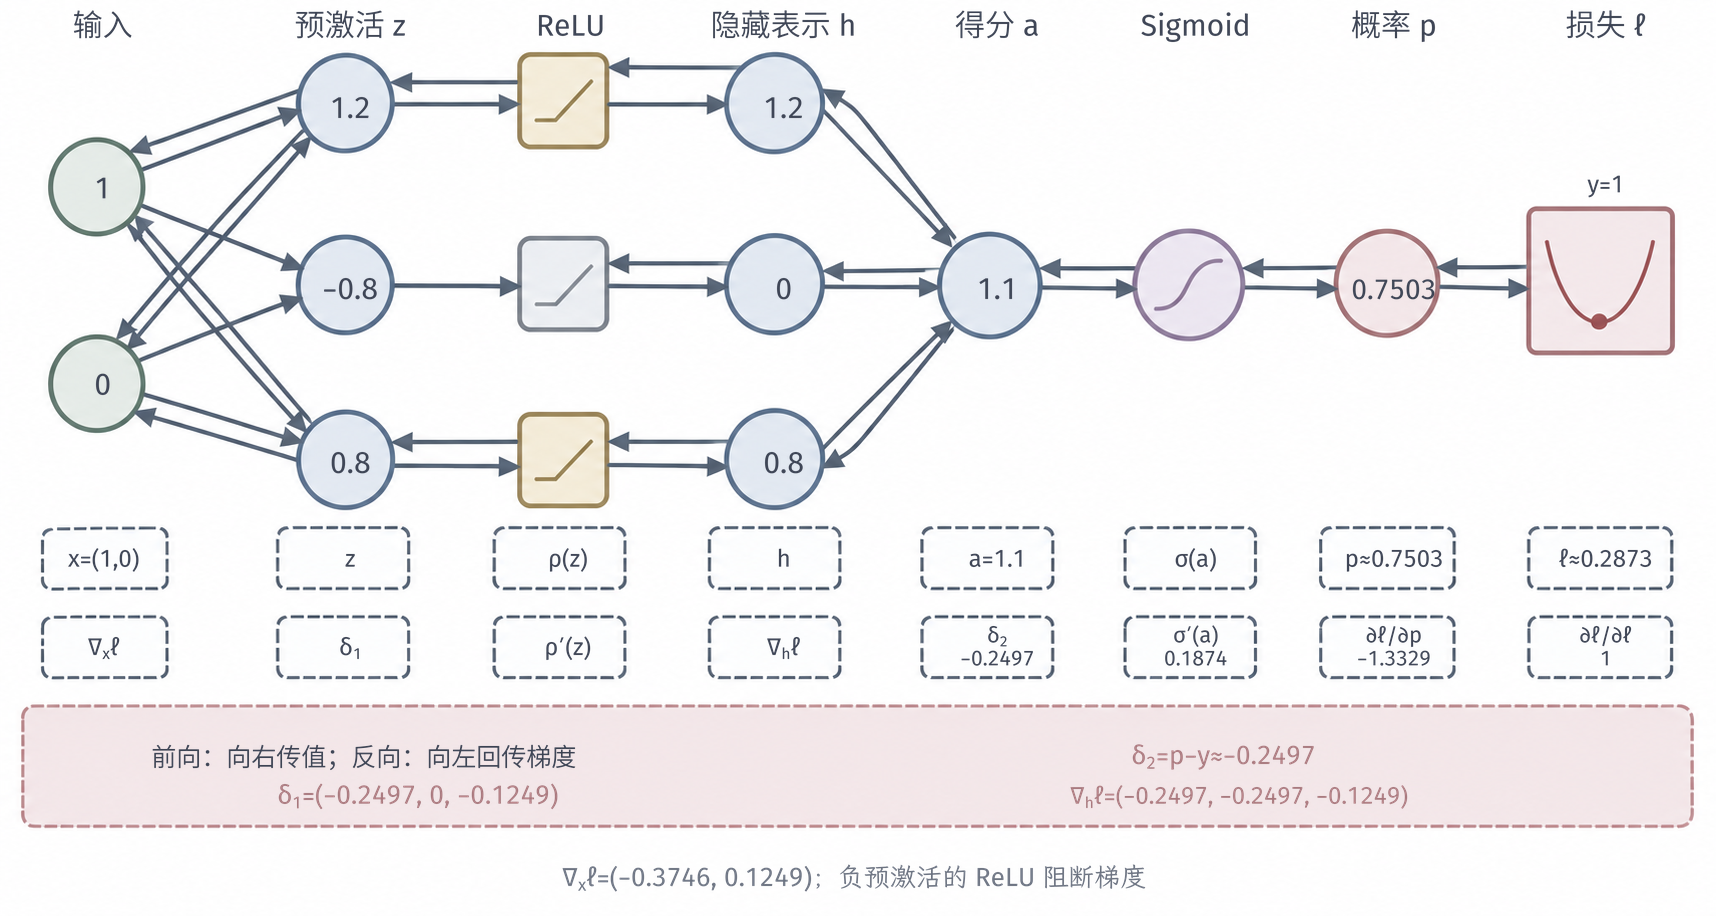
\includegraphics[width=145.288mm]{figures/03-models/02-neural-network-models/generated/ffn-backpropagation/figure.png}
  \caption{示例~\ref{ex:ffn-numerical-backpropagation}中$2$-$3$-$1$网络的计算图。上方节点和下方第一行给出前向值，第二行及红色汇总给出反向量；箭头方向区分前向传值与反向回传梯度；预激活与隐藏表示是同一隐藏层的两种数值，不是两个隐藏层。下方红色虚线按向量形式汇总梯度，坐标顺序与上方节点从上到下一致。第三个单元通过输出权重$0.5$收到梯度，第二个单元的梯度被负半轴上的ReLU截断。数值按更新前参数计算，梯度和概率保留四位小数。}
  \label{fig:ffn-backpropagation}
\end{figure*}

\begin{example}[一次前向与反向计算]
  \label{ex:ffn-numerical-backpropagation}
  沿用异或的二值输入，使用图~\ref{fig:neural-minimal-mlp}中的$2$-$3$-$1$结构：一个隐藏层含三个ReLU单元，输出得分经Sigmoid变成二分类概率。下面的参数是教学构造，不是已训练好的异或分类器：
  \[
    \begin{aligned}
      \bm{W}_1&=\begin{pmatrix}1&-1\\-1&1\\1&1\end{pmatrix},
      &\bm{b}_1&=\begin{pmatrix}0.2\\0.2\\-0.2\end{pmatrix},\\
      \bm{W}_2&=\begin{pmatrix}1&1&0.5\end{pmatrix},
      &b_2&=-0.5\text{。}
    \end{aligned}
  \]
  对样本$\bm{x}=(1,0)^{\top}$、$y=1$，前向结果为
  \[
    \begin{aligned}
      \bm{z}^{(1)}&=(1.2,-0.8,0.8)^{\top},\\
      \bm{h}^{(1)}&=(1.2,0,0.8)^{\top},\\
      a&=1\times1.2+1\times0+0.5\times0.8-0.5=1.1\text{。}
    \end{aligned}
  \]
  因而$p=s(1.1)\approx0.7503$，二元交叉熵$\ell=-\log p\approx0.2873$。本例三个预激活值都远离ReLU的不可微点，局部导数依次为$1,0,1$。

  输出敏感度为$\delta^{(2)}=p-1\approx-0.2497$。先乘输出权重的转置，再逐坐标乘激活导数，得到
  \[
    \begin{aligned}
      \nabla_{\bm{h}^{(1)}}\ell
        &\approx(-0.2497,-0.2497,-0.1249)^{\top},\\
      \bm{\delta}^{(1)}&\approx(-0.2497,0,-0.1249)^{\top},\\
      \nabla_{\bm{W}_1}\ell&\approx
      \begin{pmatrix}-0.2497&0\\0&0\\-0.1249&0\end{pmatrix},
      &\nabla_{\bm{b}_1}\ell&\approx
      \begin{pmatrix}-0.2497\\0\\-0.1249\end{pmatrix}\text{。}
    \end{aligned}
  \]
  例如第三个隐藏单元的第一条输入权重，其梯度是
  \[
    \frac{\partial\ell}{\partial(\bm{W}_1)_{3,1}}
    =(p-1)\times0.5\times1\times x_1
    \approx-0.1249\text{。}
  \]
  这四个因子依次来自输出损失、输出连接、ReLU局部导数和输入值。输出参数的梯度为$\nabla_{\bm{W}_2}\ell\approx(-0.2997,0,-0.1998)$、$\partial\ell/\partial b_2\approx-0.2497$；继续回传到输入则有$\nabla_{\bm{x}}\ell\approx(-0.3746,0.1249)^{\top}$。第一层第一、第三个单元对$x_2$的权重梯度为零，是因为这个样本的$x_2=0$；第二个单元的输入权重梯度为零，则来自负半轴上的激活导数。两种零梯度有不同原因。

  若仅用该样本、不加正则项，并以学习率$0.1$同时更新所有参数，即每项参数减去$0.1$倍的对应梯度，则更新后的参数为
  \[
    \begin{aligned}
      \bm{W}_1^{(1)}&\approx
        \begin{pmatrix}1.0250&-1\\-1&1\\1.0125&1\end{pmatrix},
      &\bm{b}_1^{(1)}&\approx
        \begin{pmatrix}0.2250\\0.2\\-0.1875\end{pmatrix},\\
      \bm{W}_2^{(1)}&\approx\begin{pmatrix}1.0300&1&0.5200\end{pmatrix},
      &b_2^{(1)}&\approx-0.4750\text{。}
    \end{aligned}
  \]
  参数上标$(1)$表示一次更新。用未舍入的梯度重算该输入，隐藏表示约为$(1.2499,0,0.8250)^{\top}$，得分约为$1.2414$，正类概率约为$0.7758$，损失约为$0.2539$。本次下降只针对更新所用的正例；全部异或样本的总损失与新样本风险，需要分别用相应样本或分布评价。
\end{example}

训练目标通常包含多个样本，它们共享同一组参数，因此梯度需要相加。若本次更新读取一个索引集合$B\subseteq\{1,\ldots,n\}$，称为\term{小批量}（mini-batch），其平均数据梯度为
\begin{equation}
  \bm{G}_\ell=
  \frac1{|B|}\sum_{i\in B}
  \bm{\delta}_i^{(\ell)}(\bm{h}_i^{(\ell-1)})^{\top},
  \qquad
  \bm{r}_\ell=
  \frac1{|B|}\sum_{i\in B}\bm{\delta}_i^{(\ell)}\text{。}
  \label{eq:ffn-minibatch-gradients}
\end{equation}
这里$\bm{G}_\ell\in\mathbb R^{d_\ell\times d_{\ell-1}}$是权重梯度矩阵，$\bm{r}_\ell\in\mathbb R^{d_\ell}$是偏置梯度向量。每个样本的$\bm{\delta}_i^{(\ell)}$按未除以批量大小的单样本损失计算。若反向起点已经使用批平均损失，所得敏感度已经包含按$|B|$取平均的缩放。矩阵实现可将样本按列排列，用同样的矩阵乘法一次计算这些外积之和；样本按行排列的实现会相应改变转置位置。

若$\Omega=\frac12\sum_\ell\lVert\bm{W}_\ell\rVert_{\mathrm{F}}^2$，其中$\lVert\cdot\rVert_{\mathrm{F}}$是矩阵各元素平方和开方得到的Frobenius范数，则权重总梯度为$\bm{G}_\ell+\lambda\bm{W}_\ell$，未被惩罚的偏置不加这一项。给定学习率$\eta_t>0$，普通梯度更新为
\begin{equation}
  \begin{aligned}
    \bm{W}_\ell^{(t+1)}
      &=\bm{W}_\ell^{(t)}-\eta_t(\bm{G}_\ell+\lambda\bm{W}_\ell^{(t)}),\\
    \bm{b}_\ell^{(t+1)}&=\bm{b}_\ell^{(t)}-\eta_t\bm{r}_\ell\text{。}
  \end{aligned}
  \label{eq:ffn-gradient-update}
\end{equation}
这里迭代上标$t$与层下标$\ell$分别记录训练时刻和结构位置。

\begin{algorithm}[前馈网络的小批量梯度学习]
  \label{alg:ffn-minibatch-learning}
  \begin{algorithmic}[1]
    \Require 训练集$S$、验证集、网络结构、损失、学习率序列与停止规则
    \Ensure 经验证集选择的参数$\bm{\theta}$
    \State 按激活与层宽初始化权重，初始化偏置
    \While{尚未达到停止规则}
      \State 读取小批量$B$，保存各样本的预激活、隐藏表示与输出
      \State 计算输出敏感度$\bm{\delta}_i^{(L+1)}$
      \For{$\ell=L,L-1,\ldots,1$}
        \State 按式\eqref{eq:ffn-backward-recursion}计算$\bm{\delta}_i^{(\ell)}$
      \EndFor
      \State 汇总所有层的数据梯度，并加入所选惩罚项的梯度
      \State 使用同一更新前参数计算的梯度，同时更新各层参数
      \State 按既定间隔评估验证集，记录待选择的参数
    \EndWhile
    \State 返回按预先规定验证指标选择的参数
  \end{algorithmic}
\end{algorithm}

算法~\ref{alg:ffn-minibatch-learning}把求导和更新分成两步。如果在尚未完成反向计算时就改写某层权重，前后各层的梯度可能对应不同的参数，便不再是同一个目标在同一点的梯度。停止规则可以包含最大更新次数和验证指标的停止条件；优化器、学习率安排及更广泛的训练问题将在训练章比较。

反向传播的计算量与前向矩阵运算同阶，因为每层主要计算转置矩阵乘法和外积，而不是为每个参数重新运行网络。它通常还要保存各层的活动值，单样本隐藏激活的存储量与$\sum_\ell d_\ell$同阶，小批量时随批量大小增长。逐层导数相乘也解释了小梯度和大梯度如何累积：这种乘积可以使正确计算出的梯度很小或很大，更新效果还取决于它的实际尺度。

用十次连乘就能看清这种累积。只考虑一条经过$10$个Sigmoid单元的标量路径，并假设路径上各权重的绝对值不超过$1$。由于每个激活导数至多为$0.25$，沿这条路径回传的敏感度，其绝对值至多乘上
\[
  0.25^{10}=\frac{1}{1048576}\approx9.54\times10^{-7}\text{。}
\]
这一上界针对指定标量路径。完整网络还需要相加各路径贡献，权重幅度也会参与信号缩放。对串联的$10$个Sigmoid向量层，若各层权重矩阵的谱范数均不超过$1$，回传向量穿过这$10$层后，其范数也至多乘上这个因子。谱范数衡量一次线性变换对向量长度的最大放大倍数，每项权重不超过$1$只约束单个元素，许多元素共同作用时谱范数仍可能较大。梯度经过多层后变得很小、使上游参数难以获得有效更新，称为\term{梯度消失}（vanishing gradients）。

反过来，若一条标量路径经过$10$个处于正半轴的ReLU单元，每条权重均为$2$，则这些单元的激活导数为$1$，路径上的回传倍数为$2^{10}=1024$。这是权重与激活状态持续配合造成的放大，展示了\term{梯度爆炸}（exploding gradients）的机制；完整梯度的放大则取决于沿途所有权重、激活状态及路径贡献。两种算术都将梯度尺度落实为沿路径的乘积：可导性提供局部变化率，连乘及汇总决定最终回传量。

\subsection{自动梯度计算}
\label{sec:ffn-autodiff}

普通串联网络的梯度可以手工推导，但模型加入多个分支、共享参数或额外损失以后，逐项维护公式很容易遗漏一条影响路径。要把求导交给程序，需要说明程序到底在算什么。数值微分、符号微分和自动微分都能提供导数信息，采用的原理却不同。

\term{数值微分}（numerical differentiation）通过改变输入后观察函数值之差来近似导数。例如，用第$j$个标准基向量$\bm{e}_j$和步长$\varepsilon>0$，中心差分为
\begin{equation}
  \frac{\partial J}{\partial\theta_j}
  \approx
  \frac{J(\bm{\theta}+\varepsilon\bm{e}_j)
       -J(\bm{\theta}-\varepsilon\bm{e}_j)}{2\varepsilon}\text{。}
  \label{eq:ffn-finite-difference}
\end{equation}
在足够光滑且附近高阶导数受控时，其截断误差随$\varepsilon^2$缩小；步长过小时，两次接近的函数值相减又会放大浮点误差。得到$p$个参数的完整梯度通常需要约$2p$次目标计算，所以它适合检查少量梯度或方向导数，不适合直接承担大网络的每次更新。检查ReLU网络时应避开激活切换点，否则差分可能跨越两个不同的线性区域。

\term{符号微分}（symbolic differentiation）按照求导规则变换表达式，例如把$\frac12(uv+u)^2$变成关于$u,v$的导数公式，再在某一点求值。它能给出可以继续分析的表达式，但未经简化和公共子表达式复用时，复杂复合函数的导数表达式可能迅速膨胀。符号方法也可以利用共享结构；这些复用会减少重复展开，实际规模取决于表达式组织与实现。

\term{自动微分}（automatic differentiation, AD）把程序实际执行的计算拆成具有已知局部导数的基本运算，在计算数值的同时或之后应用链式法则。它不通过有限扰动估计导数，也不必先展开整个导数表达式。若所执行运算可微且局部求导规则正确，所得结果是这条计算路径的导数在当前点的数值，仍受浮点舍入影响；舍入误差和不可微操作仍分别由数值精度与所执行的算子决定。

\subsubsection{算子图与前向模式}
\label{sec:ffn-autodiff-forward}

为了区分两种传播方向，考虑教学函数$J(u,v)=\frac12(uv+u)^2$。把计算拆成$r=uv$、$s=r+u$、$t=s^2$和$J=t/2$，就得到乘法、加法、平方与缩放四个算子。每个算子只读取前面已经得到的值，输入$u$则分别进入乘法和加法，形成两条影响输出的路径。

\term{前向模式}（forward mode）随前向值一起传播某个输入方向上的变化率。若点上的输入方向为$(\dot u,\dot v)$，有
\begin{equation}
  \begin{aligned}
    \dot r&=v\dot u+u\dot v,&\dot s&=\dot r+\dot u,\\
    \dot t&=2s\dot s,&\dot J&=\tfrac12\dot t\text{。}
  \end{aligned}
  \label{eq:ffn-forward-mode}
\end{equation}
圆点表示沿所选方向的导数，不表示时间演化。取$u=2,v=3$，前向值依次为$r=6,s=8,t=64,J=32$。如果选择$(\dot u,\dot v)=(1,0)$，表示只沿$u$的正方向考察变化：乘法给出$\dot r=3$，加法还收到$u$直接传来的$1$，于是$\dot s=4$；经过平方与缩放，得到$\dot t=64$、$\dot J=32$。

\begin{figure*}[htb]
  \centering
  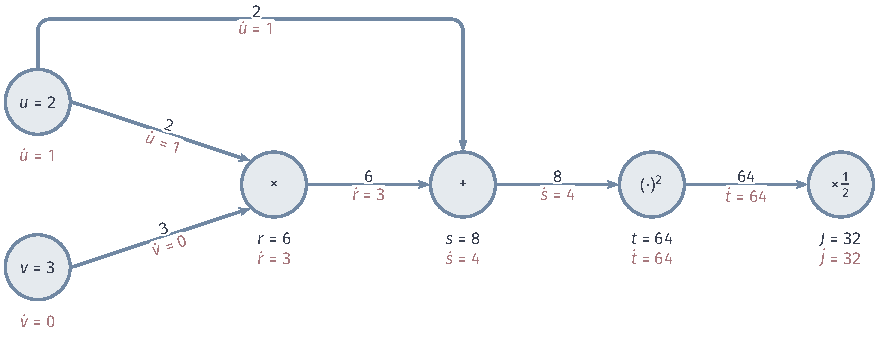
\includegraphics[width=148.791mm]{figures/03-models/02-neural-network-models/tikz/ffn-autodiff-forward/figure.pdf}
  \caption{具体算子图上的前向模式。圆形节点表示乘法、加法、平方和缩放；实线上方的前向数字是传入算子的值，下方红色数字是同一路径上的方向导数。每个算子下方再用两行列出其输出值和输出方向导数。输入方向$(1,0)$给出$\partial J/\partial u=32$；加法处的$\dot s=3+1$包含了$u$的两条路径。}
  \label{fig:ffn-autodiff-forward}
\end{figure*}

图~\ref{fig:ffn-autodiff-forward}把一次方向导数计算附在原有算子图上。若要计算对$v$的偏导，改取$(\dot u,\dot v)=(0,1)$：此时$\dot r=2$、$\dot s=2$、$\dot t=32$，最终$\dot J=16$。两次遍历的前向值相同，变化的是输入方向以及随之传播的导数。

\FloatBarrier
\subsubsection{后向模式与梯度累加}
\label{sec:ffn-autodiff-reverse}

若希望从一个标量目标同时得到多个输入的导数，可以反过来问：输出对当前中间值有多敏感？\term{后向模式}（reverse mode）从输出向输入累积这种敏感度。记$\bar r=\partial J/\partial r$，对其他变量采用相同横线记号；前向值仍保留在原算子图中，从$\bar J=1$开始回传：
\begin{equation}
  \begin{aligned}
    \bar t&=\tfrac12\bar J,&\bar s&=2s\bar t,\\
    \bar r&=\bar s,&\bar u&=\bar r v+\bar s,\\
    &&\bar v&=\bar r u\text{。}
  \end{aligned}
  \label{eq:ffn-reverse-mode}
\end{equation}
每条回传贡献等于下游敏感度乘该条依赖的局部导数。缩放算子给出$\bar t=1/2$，平方算子利用保存的$s=8$得到$\bar s=8$，加法向两个输入各传递$8$。其中传给$r$的$8$再经过乘法，分别给$u$和$v$贡献$8v=24$与$8u=16$。

\begin{figure*}[htb]
  \centering
  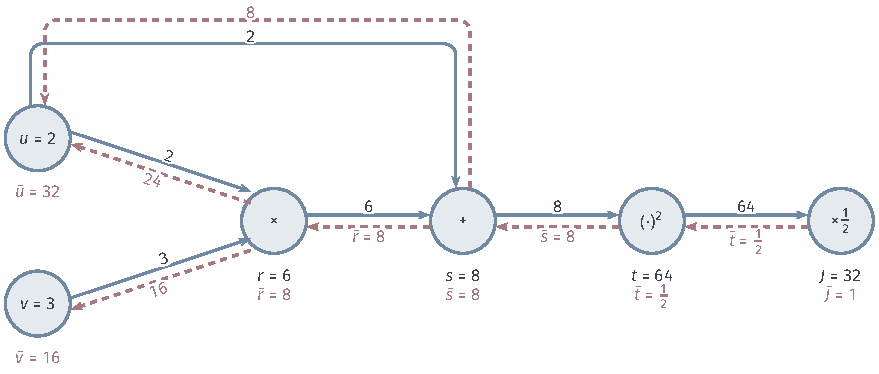
\includegraphics[width=148.791mm]{figures/03-models/02-neural-network-models/tikz/ffn-autodiff-reverse/figure.pdf}
  \caption{同一算子图上的后向模式。节点位置与前向模式相同，实线及其前向标注保留前向传递值，红色虚线及其标注从$\bar J=1$开始回传导数贡献；每个算子下方两行分别给出输出值和伴随值。输入$u$收到经乘法传来的$24$和直接经加法传来的$8$，累加为$32$；输入$v$得到$16$。一次后向遍历同时得到两个偏导。}
  \label{fig:ffn-autodiff-reverse}
\end{figure*}

在图~\ref{fig:ffn-autodiff-reverse}中，$u$有两条通向目标的路径，所以$\bar u=24+8=32$。若漏掉直接进入加法的路径，就会错误地得到$24$。共享参数在多处被使用时也遵循同样规则：先保存各使用位置的局部回传贡献，再把它们累加到同一个参数。后向模式改变的是求导顺序，原函数的前向依赖并没有改变。

\FloatBarrier
\subsubsection{两种模式的计算代价}
\label{sec:ffn-autodiff-cost}

对一般映射$\bm{F}:\mathbb{R}^{p}\to\mathbb{R}^{q}$，Jacobian矩阵$\bm{J}_{\bm{F}}\in\mathbb{R}^{q\times p}$的行对应输出坐标、列对应输入坐标，梯度采用列向量。前向模式在给定输入方向$\bm{v}\in\mathbb{R}^{p}$时计算$\bm{J}_{\bm{F}}\bm{v}$，后向模式在给定输出权重$\bm{u}\in\mathbb{R}^{q}$时计算$\bm{J}_{\bm{F}}^{\top}\bm{u}$。二者都可直接计算乘积，无需存储完整Jacobian矩阵。用逐坐标方向构造完整Jacobian矩阵时，前向模式需要$p$个方向，后向模式需要$q$个方向；实际代价还取决于批处理、稀疏结构和基本算子的实现。

神经网络训练通常有很多参数，却只有一个标量目标，即$q=1$。后向模式从该目标出发，能够在与前向求值同阶的算术工作中得到完整参数梯度，代价是保存或重新计算反向所需的中间值。前述反向传播就是后向模式在神经网络损失上的具体应用\scite{baydin2018autodiff}

如果计算图包含多条损失分支，梯度在共同上游节点相加；如果某些分支被有意停止求导，它们就不再贡献上游梯度。离散采样、取整和按值选择分支也需要分别判断可微性：自动微分通常沿当前执行路径应用已登记的规则，不会自行补上对离散选择概率的导数。核验所得梯度时，需要同时检查目标、依赖路径和特殊算子的求导规则；数值梯度检查可进一步检验选定点附近的计算。

\section{理论分析}
\label{sec:ffn-theory}

理论分析分别回答三个问题：候选网络能否逼近目标，训练能否找到足够好的候选，以及选出的候选能否在新样本上保持低风险。表达能力、收敛性与泛化性对应这三个问题，所需条件不能互相替代。

\subsection{表达能力}
\label{sec:ffn-expressivity}

前章的异或例子是一个精确表示结论：指定输入集合上存在某组参数，输出规则与标签一致。面对一般连续输入，常见问题则是能否让网络与目标函数的误差足够小。\term{表达性}（expressivity）描述网络族能够表示或逼近哪些函数；它的判断对象是整类可选参数形成的函数，而不是某次训练得到的参数。

在非空紧输入集上，对连续目标使用连续非多项式激活、隐藏偏置与线性输出，
给定精度后可选择有限宽度和参数，使一致误差小于该精度。
本章的Sigmoid、Tanh、ReLU、GELU与SiLU满足这些激活条件。
这条存在性结论允许宽度和参数随精度改变（参考\BookTheoremRef{thm:functional-universal-approximation}{第一卷“数学准备”的“单隐藏层的通用逼近”定理}）。固定层宽和参数范数时可表示的范围更受限制；训练求解与域外预测又分别依赖算法和数据条件。
下面关注前馈结构怎样利用宽度与深度组织这些表示。

ReLU网络的一个直接读法是分段仿射变换。在一组隐藏单元的正负状态固定的输入区域内，所有ReLU都等价于保留某坐标或置零，整个网络因而是仿射的。不同激活状态形成不同区域，区域边界随参数改变。它能拼接出复杂形状，但固定有限网络仍只有有限个这样的区域。

一维情形能把这种拼接写成明确公式。设连续分段线性函数的内部转折点为$t_1<\cdots<t_m$，从左到右的斜率为$s_0,s_1,\ldots,s_m$，则可写成
\begin{equation}
  f(x)=c+s_0x+
  \sum_{j=1}^{m}(s_j-s_{j-1})\rho(x-t_j)\text{。}
  \label{eq:ffn-piecewise-linear-representation}
\end{equation}
每个ReLU在一个转折点之后改变斜率；常数$c$确定整体高度。若标准MLP不含直接的线性输入支路，可以用$x=\rho(x)-\rho(-x)$补出$s_0x$。因此宽度确实可以增加可表达的转折，而不只是抽象地增加参数。对紧区间上的连续函数取足够密的插值节点，再作分段线性插值，也给出了ReLU通用逼近在一维中的构造直觉。

深度提供另一种组织复杂函数的方式：重复复用已有变换。考虑$[0,1]$上的三角形函数
\begin{equation}
  T(x)=2\rho(x)-4\rho(x-1/2)+2\rho(x-1)\text{。}
  \label{eq:ffn-tent-function}
\end{equation}
它在$[0,1/2]$从$0$上升到$1$，在$[1/2,1]$再下降到$0$。令$T_k$表示$T$复合$k$次，而不是$T$的$k$次幂。$T_1$有两个线性区间，每个区间都把输入完整地送到$[0,1]$；再次应用$T$就把每个区间分成两段。归纳可得$T_k$在$[0,1]$有$2^k$个线性区间。

\begin{figure*}[htb]
  \centering
  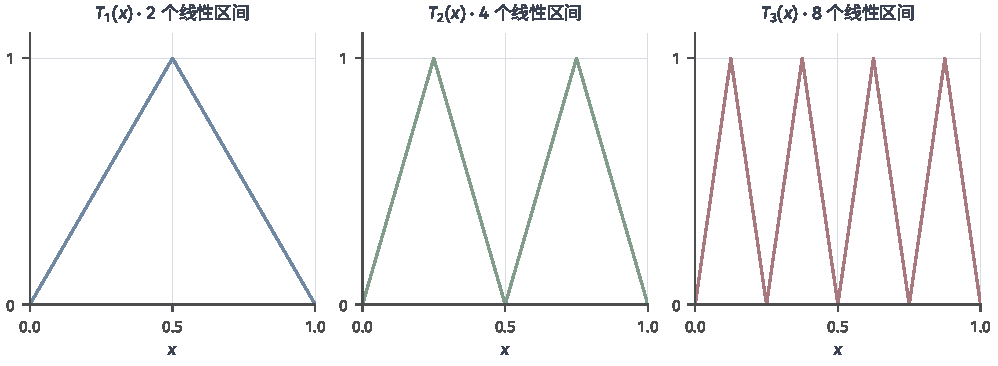
\includegraphics[width=159.059mm]{figures/03-models/02-neural-network-models/matplotlib/ffn-depth-composition/figure.pdf}
  \caption{三角形函数的复合产生更多转折。三幅解析图分别为$T_1=T$、$T_2=T\circ T$和$T_3=T\circ T\circ T$，横轴均为$x\in[0,1]$，纵轴为函数值。每次复合将线性区间数翻倍；这是一维构造，不是实际训练实验，也不表示任意目标都能从增加深度中获得相同收益。}
  \label{fig:ffn-depth-composition}
\end{figure*}

把$T$的三个ReLU响应与线性组合逐次串联，可以用深度随$k$线性增长、每层宽度有常数上界的网络表示$T_k$；相邻线性映射可合并到下一层权重中。单隐藏层的一维ReLU网络中，每个单元至多引入一个内部转折，所以要精确表示具有$2^k$个线性区间的$T_k$，至少需要$2^k-1$个隐藏单元。图~\ref{fig:ffn-depth-composition}展示了这种重复组合的效率。更一般的深度分离结果还需固定误差度量、目标函数族和比较网络的范围\scite{telgarsky2016depth}

这个例子固定同一个三角形复合目标，比较浅层与深层表示所需的单元数；训练难度和新样本风险是另外两个评价对象。某些目标用浅层结构已经足够；若目标本身具有可复用的组合规律，深度才可能以较少单元组织这种规律。表达能力的分析因此应同时说明目标、激活、深度、宽度和逼近精度。

\subsection{收敛性}
\label{sec:ffn-convergence}

隐藏层参数与输出权重同时训练时，经验目标通常非凸。精确表示参数的存在提供一个候选解，迭代能否到达它还取决于初始化、目标几何与梯度尺度。对于有下界的确定性目标、沿迭代区域具有$\beta$-Lipschitz梯度的情形，采用固定的正步长、且步长不超过$1/\beta$时，梯度下降可以把已计算迭代点中梯度范数平方的最小值控制到$O(1/T)$，其中$T$为更新次数。这个速率衡量梯度接近零的程度；驻点是否全局最优还需目标的其他性质。

若只训练固定隐藏特征上的平方损失读出，问题成为凸二次优化；若将样本作为行、固定特征及待估偏置对应的常数项作为列，设计矩阵各列线性无关，或对全部待估系数加入正的岭惩罚，就能保证唯一读出解。隐藏特征固定使目标对读出参数保持二次形式；同时训练隐藏参数时，特征也随更新改变。全网络获得全局收敛通常需要额外的结构、初始化或过参数化条件，宽度只有与这些条件一起进入分析时，才支持相应的收敛结论。学习率、梯度随机性、曲率与停止准则在第\ref{chap:neural-network-training}章统一分析。

\subsection{泛化性}
\label{sec:ffn-learnability}

通用逼近允许观察目标函数之后选择参数，而训练只能看到有限个样本。网络可以在这些样本之间构造许多不同的延伸，未见输入上的表现也就可能不同。\term{可学习性}考察给定任务、数据假设和学习方式时，样本能否支持低风险的预测规则。统计上需要多少样本、计算上能否找到合适参数，分别需要复杂度和优化方面的依据。

沿用机器学习理论基础章的统一设定，假设训练样本独立同分布地来自$\mathcal{P}$，测试样本也来自同一分布。对事先确定的网络函数空间$\mathcal{H}$，记期望风险为$R(f)=\mathbb{E}_{\mathcal{P}}\ell(f(\bm{x}),y)$、经验风险为$\widehat R_S(f)$，学习算法的输出为$\widehat f=A(S)\in\mathcal{H}$。若对所有$f\in\mathcal{H}$同时有$|R(f)-\widehat R_S(f)|\leq\Delta$，且算法的经验优化误差至多为$\xi$，则
\begin{equation}
  \begin{aligned}
    R(\widehat f)-R^*\leq{}&
    \underbrace{\inf_{f\in\mathcal{H}}R(f)-R^*}_{\text{逼近误差}}\\
    &+\underbrace{2\Delta}_{\text{估计误差的控制}}
    +\underbrace{\xi}_{\text{优化误差}}\text{。}
  \end{aligned}
  \label{eq:ffn-risk-decomposition}
\end{equation}
这里$R^*$是同一损失下允许所有可测预测规则得到的最优风险，$\xi$满足$\widehat R_S(\widehat f)\leq\inf_{f\in\mathcal{H}}\widehat R_S(f)+\xi$。把$\widehat f$的经验风险与某个近似最优比较函数的经验风险连接起来，再分别用一致偏差$\Delta$替换为期望风险，就得到该式。对于无界损失，要建立这样的统一界还需矩或尾部等额外条件。

这三项解释了增加模型规模的不同作用：更大的函数空间可能降低逼近误差，却会改变估计误差的控制；更深的计算也可能使优化误差难以降低。式\eqref{eq:ffn-risk-decomposition}给出了这些因素进入风险上界的途径；上界能否接近真实风险，还取决于复杂度控制的精度。参数量改变时三项可能同时变化，测试误差因此需要结合它们判断。

输入维度通过表示规模与数据几何共同起作用。若每个坐标都满足$|x_j|\leq c$，只能粗略保证$\lVert\bm{x}\rVert_2\leq c\sqrt d$，因而以输入范数为依据的界可能随$d$变大；若输入整体已归一化，或数据只占据较低维的有效区域，维度的作用就不能只按坐标数判断。但低维分布本身也不保证任务简单：标签可能在该区域内变化得很复杂，还可能含有噪声。输入分布、目标结构和损失应在同一分析中固定。

样本量与权重尺度的作用可以用受范数约束的两层ReLU得分具体展示。此处改用标签$y\in\{-1,+1\}$和标量分类得分，讨论不含偏置的函数
\[
  f(\bm{x})=\sum_{j=1}^{m}a_j\rho(\bm{w}_j^{\top}\bm{x}),
  \qquad \sum_{j=1}^{m}|a_j|\leq A,
  \qquad \lVert\bm{w}_j\rVert_2\leq B\text{。}
\]
在抽样前固定$A,B,r,\gamma>0$，并假定$\lVert\bm{x}\rVert_2\leq r$。以至少$1-\delta$的概率，上述函数同时满足
\begin{equation}
  \begin{aligned}
    \mathbb{P}_{\mathcal{P}}\{yf(\bm{x})\leq0\}
    \leq{}&\frac1n\sum_{i=1}^{n}
      \mathbb{I}\{y_i f(\bm{x}_i)\leq\gamma\}\\
    &+\frac{4ABr}{\gamma\sqrt n}
      +3\sqrt{\frac{\log(2/\delta)}{2n}}\text{。}
  \end{aligned}
  \label{eq:ffn-margin-risk}
\end{equation}
其中$\gamma$是要求训练样本达到的正分类间隔，$\delta\in(0,1)$是允许保证失效的概率（推导参考\BookTheoremRef{thm:two-layer-norm-risk}{第二卷“基础、理论和可信性”的“深度学习的可学习性”章“两层网络的范数与期望风险”定理}）。左侧把零间隔也计为错误，因而可控制固定平局规则下的分类风险。右侧既包含未达到间隔的训练样本比例，也包含从有限样本推断新样本时的复杂度代价；达到正间隔比仅分对训练样本提出了更强要求，这一差别使间隔与复杂度能够在同一个界中联系起来。

在$A,B,r,\gamma,\delta$固定时，将样本量增至四倍，会把后两项减半。这一缩放作用于充分界的复杂度项，实际错误率由所选函数与测试分布决定。它也说明为什么要区分独立样本与重复记录：把同一条记录复制四次没有产生这项独立同分布保证所要求的新信息。

参数范数与间隔需要一起看。把所有输出权重乘以一个很小的正数，会缩小$A$，但也按相同比例缩小分类间隔，分类符号并不改变；界中的范数与间隔因而需要同时比较。若在保持函数不变的前提下，将某个ReLU隐藏单元的输入权重乘$c>0$、输出权重除以$c$，不同层的原始范数同样会变化。分析应采用与函数、间隔及参数化相配的复杂度量。

式\eqref{eq:ffn-margin-risk}没有显式出现隐藏宽度$m$，因为总输出权重和各隐藏权重范数已经受到限制。增加宽度提供更多候选特征，而总输出权重与各隐藏权重仍受既定限制。如果宽度增加时$A$、$B$也增加，或有效间隔变小，界仍会变差。允许所有宽度和任意权重的分类函数空间又可能具有无限VC维，其分布无关PAC结论需要另一组容量条件，有范数与间隔限制的界覆盖的是这里指定的子类。固定有限ReLU架构的VC分析还需按参数数、层数与计算单元数给出容量条件（分析与统计学习结论参考\BookChapterRef{chap:deep-learning-theory}{第二卷“基础、理论和可信性”的“深度学习的可学习性”章}）。

深度影响层间扰动的放大。对本章的串联网络，若隐藏激活均为$1$-Lipschitz，即不会增大两点之间的欧氏距离，原始输出映射满足
\begin{equation}
  \lVert\bm{a}(\bm{x})-\bm{a}(\bm{x}')\rVert_2
  \leq
  \left(\prod_{\ell=1}^{L+1}\lVert\bm{W}_\ell\rVert_2\right)
  \lVert\bm{x}-\bm{x}'\rVert_2\text{。}
  \label{eq:ffn-input-sensitivity}
\end{equation}
这里矩阵谱范数$\lVert\bm{W}_\ell\rVert_2$表示线性变换对向量长度的最大放大倍数。每层分别使用这一上界，再沿函数复合相乘，便得到该式；有其他Lipschitz常数的激活还需乘上相应因子。偏置在比较同一层的两个输入时相消，但它仍会影响激活区域及函数空间的复杂度。

式\eqref{eq:ffn-input-sensitivity}比较同一固定网络在两个输入上的变化。泛化分析则比较训练所得函数的经验风险与期望风险，还需要候选范围及抽样条件。深层谱复杂度分析还结合各层其他范数、输入尺度和分类间隔；比较层数时，本章只计隐藏层，所引用分析的总层数还包括线性输出层（具体条件参考\BookSectionRef{sec:network-norm-bounds}{第二卷“基础、理论和可信性”的“深度学习的可学习性”章“基于参数大小的可学习性”节}）。
它说明深度不能只作为层数进入判断：层间尺度的乘积、可复用目标结构以及训练能否得到合适表示，都可能同时变化。

学习算法决定从许多低训练损失参数中选择哪一个解。更新形成选解偏好，初始梯度特征规定最初可用的学习方向，分别在相应条件下描述这种选择（参考\BookSectionRef{sec:implicit-bias}{第二卷“基础、理论和可信性”的“深度学习的可学习性”章“基于参数梯度更新的可学习性”节}和\BookSectionRef{sec:neural-tangent-kernel}{第二卷“基础、理论和可信性”的“深度学习的可学习性”章“基于参数梯度初始值的可学习性”节}）。初始化、更新方式、正则化和停止时刻既可能影响经验优化误差，也可能影响输出对样本替换的敏感性。若算法具有损失均匀稳定性$\beta_n$，且相关训练、测试及样本替换后的损失可积，其期望泛化差可受$\beta_n$控制（参考\BookTheoremRef{thm:stability-expected-generalization}{第二卷“基础、理论和可信性”的“一般学习的可学习性”章“均匀稳定性与期望风险”定理}）。这里对独立同分布训练样本取期望；随机算法还需在独立内部随机性平均的同一口径下建立稳定性并评价泛化差。这一比较固定学习算法，改变一条训练样本并比较两个训练结果；同一次训练的相邻更新所改变的对象不同。

因此，从前馈结构得到学习判断，需要把任务、样本分布、候选函数约束和算法放在一起。独立同分布风险界不直接覆盖部署分布改变，交叉熵降低也不直接等于零一风险保证。完整的风险论证将目标函数的逼近误差、有限样本的估计控制和算法的经验优化误差连接起来，再按任务损失解释最终风险。

\section{常见应用}
\label{sec:ffn-applications}

前馈网络既可以直接完成固定长度输入的预测，也可以在更大的模型中承担一段变换。完整应用由输入编码、网络计算、训练目标和输出决策共同组成；以下固定任务，把这些环节连接起来。

\subsection{表格数据的分类与回归}
\label{sec:ffn-tabular}

表格中的一行通常描述一个对象，不同列分别记录数值或类别属性。网络接收的是定长数值向量，所以必须先规定每列怎样进入向量。数值列可按训练集统计量标准化，类别列可编码成互斥的指示坐标，缺失值则需规定填充值并酌情加入缺失标记。这些规则也属于模型使用过程：验证集、测试集和新样本使用训练阶段已经确定的转换，不重新用测试数据估计均值和方差。

考虑一个教学任务：由设备使用时长、近期告警次数和三个设备类别之一，预测下一段时间是否发生故障。设两个数值变量标准化为$\widetilde x_1,\widetilde x_2$，设备类别编码为$\bm{c}\in\{0,1\}^{3}$且坐标和为$1$，输入为
\[
  \bm{x}=(\widetilde x_1,\widetilde x_2,c_1,c_2,c_3)^{\top}
  \in\mathbb{R}^{5}\text{。}
\]
采用宽度为$16$和$8$的两个ReLU隐藏层、一个标量输出，可以把完整模型写为
\begin{equation}
  \begin{aligned}
    \bm{h}^{(1)}&=\rho(\bm{W}_1\bm{x}+\bm{b}_1),\\
    \bm{h}^{(2)}&=\rho(\bm{W}_2\bm{h}^{(1)}+\bm{b}_2),\\
    p&=s(\bm{w}_3^{\top}\bm{h}^{(2)}+b_3)\text{。}
  \end{aligned}
  \label{eq:ffn-tabular-classifier}
\end{equation}
其中$\bm{W}_1\in\mathbb{R}^{16\times5}$、$\bm{W}_2\in\mathbb{R}^{8\times16}$、$\bm{w}_3\in\mathbb{R}^{8}$，偏置维度与对应输出相同。这组层宽是示例设计，不是经过实验验证的推荐配置。

训练标签$y\in\{0,1\}$记录指定时间窗内是否发生故障，用二元交叉熵构造式\eqref{eq:ffn-training-objective}，再按算法~\ref{alg:ffn-minibatch-learning}学习参数。输入必须只包含预测时刻已知的信息；故障发生后记录的维修结果不能作为预测前的输入。若同一设备有多条记录，还需按设备和时间等关系划分数据，使评价符合预期部署场景。

预测新设备记录时，先按保存的规则得到$\bm{x}$，再计算$p$，根据验证阶段确定的决策阈值得到类别。若任务改为预测后续维修时长$y\in\mathbb{R}$，可保留输入编码与隐藏层，改用线性输出和平方损失；若必须保证非负预测，可增加相应输出约束。此时预测对象从故障事件转为维修时间，输出的单位、范围与损失也随之改变。

全连接结构允许数值与类别特征在隐藏层共同作用，但它没有自动规定某种单调关系，也没有保证类别编码在缺少样本时得到可靠估计。类别很多时，直接增加指示坐标还会扩大第一层参数量，可以考虑用可学习的低维向量表示类别，但这种表示同样需要训练数据支持。表格任务中的取舍需要固定数据划分与误差指标，比较全连接结构与适合该任务的简单模型。

\subsection{其他网络中的前馈模块}
\label{sec:ffn-modules}

当输入表示已经由其他模型得到时，前馈网络仍可以把它投影到新空间，或转换成任务输出。\term{特征投影}（feature projection）改变表示的维度或坐标组织，例如用$\bm{W}\bm{h}+\bm{b}$把$d$维向量映射到$q$维。若只是两次线性投影且中间没有非线性，它们仍可以合并为一次仿射映射；如果中间维度较小，这种参数化还会限制整体线性映射的秩。

\term{分类头}（classification head）是把已有表示转换为类别得分的末端模块。卷积编码器可以把图像压成一个向量，再接线性层或MLP得到类别得分。联合训练时，分类损失的梯度沿前馈模块继续传到编码器；若固定编码器，只更新分类头，学习的参数范围就缩小了。这两种训练选择的候选范围不同：一个允许特征与任务一起改变，另一个只在固定特征上选择读出规则。

有时模块输出的是两个对象的相关性或匹配程度。例如，将两个$d$维表示$\bm{u},\bm{v}$拼接，构成输入$[\bm{u};\bm{v}]\in\mathbb{R}^{2d}$，再计算
\begin{equation}
  \operatorname{score}(\bm{u},\bm{v})=
  \bm{w}^{\top}\sigma\!\left(\bm{W}[\bm{u};\bm{v}]+\bm{b}\right)+c\text{。}
  \label{eq:ffn-scoring-module}
\end{equation}
其中隐藏宽度为$m$，$\bm{W}\in\mathbb{R}^{m\times2d}$、$\bm{b},\bm{w}\in\mathbb{R}^{m}$、$c\in\mathbb{R}$。这个\term{评分函数}（scoring function）把对象表示转换为标量得分，概率变换和损失由匹配或排序任务决定。拼接顺序意味着交换两个输入可能改变得分；若任务要求对称性，需要在输入或计算结构中加入相应约束。

前馈模块也可以对一组位置重复使用。设第$t$个位置的表示为$\bm{h}_t\in\mathbb{R}^{d}$，用同一组参数计算
\begin{equation}
  \operatorname{FFN}(\bm{h}_t)=
  \bm{W}_2\sigma(\bm{W}_1\bm{h}_t+\bm{b}_1)+\bm{b}_2\text{，}
  \label{eq:ffn-positionwise-module}
\end{equation}
其中$\bm{W}_1\in\mathbb{R}^{m\times d}$、$\bm{W}_2\in\mathbb{R}^{d\times m}$，偏置维度与相应输出一致。这种\term{逐位置变换}（position-wise transformation）分别改变每个位置内部的特征组合，在Transformer等模型中作为一个模块使用。它读取的$\bm{h}_t$可以已经包含其他位置的信息，但这次变换本身不读取$\bm{h}_{t'}$，因而不直接建立新的跨位置交互。

位置共享参数意味着所有位置的梯度都要累积到同一组$\bm{W}_1,\bm{W}_2$，而不是为每个位置保存一份独立参数。在这类组合中，前馈模块改变每个位置内的特征，其他结构负责空间、序列或对象之间的信息交换；参数共享又让不同位置共同学习同一种变换。后续各模型章会在这一基础上讨论相应的结构假设。

\section{本章小结}
\label{sec:ffn-summary}

前馈神经网络把可学习表示落实为一条没有有向环的计算路径。全连接层组合已有坐标，非线性激活让多层复合超出仿射映射，输出变换与损失共同规定训练所要预测的对象。选择层宽和激活时，既要看能够形成怎样的函数，也要看参数量、计算量和梯度传播条件。

隐藏层的学习信号来自最终目标对它的敏感度。反向传播按链式法则逐层汇总这种影响，用局部导数和已有活动值计算所有参数梯度；自动微分将同样的原则推广到程序的实际计算路径。初始化决定起点，优化器使用梯度作出更新，二者都影响学习结果，正确求导只是完成训练的一个条件。

能够逼近目标函数、能够优化经验目标、能够用有限样本控制预测风险，仍是三个不同的要求。通用逼近解释存在怎样的参数，深度与宽度解释表示成本，复杂度和稳定性则在数据与算法条件下连接训练结果和新样本风险。前馈网络适合处理定长表示，也可作为投影、分类、评分和逐位置变换模块；遇到具有明确空间、序列或关系结构的数据时，还需判断全连接假设是否充分利用了这些规律。后续章节将在相应结构上继续建立模型。

\paragraph{扩展阅读}
Goodfellow等教材第6章展开前馈网络与反向传播，计算图中的共享依赖解释了各梯度为何累加；第8章讨论所得梯度怎样用于优化，第7章讨论正则化如何限制候选和影响学习结果。这些内容分别对应本章的计算、求解与泛化问题\scite{goodfellow2016}

\chapter{卷积神经网络}
\label{chap:convolutional-networks}

一张图像中，同一种边缘可能出现在左上角，也可能出现在右下角。把像素展平后交给全连接层，各位置分别使用自己的权重；学会识别一处边缘，并未在结构上规定如何处理另一处边缘。图像的相邻关系与局部图案的重复出现，因而提出了一个问题：怎样让网络保留空间结构，并在多个位置复用同一种识别规则？第~\ref{chap:feedforward-networks}章的多层非线性表示为此提供了基础。

卷积神经网络用共享权重处理各个局部窗口，再由非线性和层次组合形成预测。同一权重在前向计算中反复使用，学习时就要汇集这些位置传回的梯度；增加深度又改变了信息与梯度经过的路径。本章先确定局部运算及其边界约定，再说明层和跨层模块的组织、参数学习，以及这种结构在什么条件下适合目标任务。分割与着色进一步要求输出保留位置对应关系。激活函数、损失和链式法则沿用前章；统计分析把结构约束与样本风险相联系（参考\BookChapterRef{chap:deep-learning-theory}{第二卷“基础、理论和可信性”的“深度学习的可学习性”章}）。

\section{卷积神经网络概述}
\label{sec:cnn-overview}

设一张彩色图像有$224\times224$个像素，每个像素包含三个颜色数值。展平后，输入维度为$150528$；连接到$1024$个隐藏单元的全连接层，仅权重就有$154140672$个。这些权重连接每个输入坐标与每个隐藏单元，规模随输入维度成比例增加。同时，连接的定义把相邻和远隔的像素同样处理，各位置也可以学习不同的局部规则。卷积改变的正是连接范围与权重复用方式。

图像中的边缘可以由邻近像素的变化来辨认，而且同一种变化可能出现在许多位置。针对这两个特点，可以分别约束读取范围和权重复用。\term{局部感受野}（local receptive field）让一个单元只读取输入中的一个邻域，即把一次计算限定在附近的若干位置。\term{参数共享}（parameter sharing）让不同位置使用同一组权重，即将同一种局部识别规则重复应用到整张图像。局部连接确定一次计算读取哪里，参数共享确定不同位置是否使用同一规则；只限制读取范围时，各位置仍有各自的权重。

\term{卷积神经网络}（convolutional neural network, CNN）把这种共享的局部计算与非线性变换逐层组合，从数据中学习局部特征及其组合。每个位置并列保存的不同特征称为\term{通道}（channel）；彩色图像的红、绿、蓝三个分量就是三个输入通道。一个输出通道是一种局部响应在所有输出位置组成的数值平面。普通密集卷积中，每种响应使用一组覆盖全部输入通道的权重，因此$64$个输出通道需要$64$组权重，而不是指$64$个空间位置。

对三个输入通道、$64$个输出通道的$3\times3$卷积层，每组权重在三个输入平面上各覆盖一个$3\times3$窗口，权重总数为$3\times3\times3\times64=1728$，再加每个输出通道一个偏置，共$64$个。这组权重的数量由核尺寸和通道数确定。图像变大后，核在更多位置使用，参数数仍保持不变。前述全连接层输出一个隐藏向量，这里输出多张空间特征图；两个计算说明了不同的参数组织，表达能力还取决于各自保留的信息和后续组合。

共享局部规则带来一种与位置变化有关的性质。\term{平移等变性}（translation equivariance）表示输入移到哪里，输出中的对应响应也移到哪里。\term{平移不变性}（translation invariance）则表示输入平移后，输出本身保持相同。图像分类可能希望物体移动后类别不变，分割却需要轮廓随物体移动，因而需要保留位置对应关系。步长为一的卷积在无限网格上与平移可交换；有限图像的边界、下采样和最终读出会改变这一性质。从随位置移动的特征得到类别不变的输出，还需要合适的汇聚与读出；这一转换的条件见后文池化分析。

这些设计适合具有规则网格、局部相关性和重复模式的数据。图像使用二维邻域，音频波形和时间序列可以使用一维邻域，体数据可以使用三维邻域。时间预测还需限制可读取的位置，避免使用尚未发生的输入。若各坐标只是含义不同的表格字段，交换相邻字段通常会改变含义，同一个局部规则也未必能沿字段排列重复使用。卷积的适用性取决于这些结构是否与任务相符。

局部处理与逐层汇聚的思想早于今天的大规模深度学习。Fukushima于1980年提出的Neocognitron交替组织局部模式检测与汇聚，使高层能够组合低层响应，并容忍一定的位置变化。它借鉴视觉系统的分层处理，但采用的学习机制与今天端到端反向传播的CNN不同；第~\ref{sec:neural-biological-system}节已介绍这条视觉启发线索\scite{fukushima1980}
到20世纪90年代，LeCun等将可学习卷积、降采样和梯度学习结合，用于手写字符和文档识别。1998年的LeNet-5展示了从像素到类别联合学习的完整系统：任务损失同时决定局部特征与后续分类。多层结构已进入实际识别系统，大规模视觉训练所需的数据和计算条件仍在发展\scite{lecun1998}

卷积结构解决了连接组织问题，深层网络能否有效训练仍是另一道关口。2006年，Hinton、Osindero和Teh提出深度信念网络的逐层学习方法：先学习一层隐表示，再把该表示作为下一层的训练数据，并对整个生成模型作后续微调。\term{逐层预训练}就是先分别为各层寻找有用的初始表示，减少从随机参数同时训练全部层的困难。这项工作为研究深层表示提供了可操作的训练途径，是理解随后深度学习兴起的一项重要进展。它研究的是生成式深层模型，原文的微调采用对比形式的wake--sleep算法，与后来判别式CNN的直接监督训练具有不同的目标和步骤\scite{hinton2006deepbelief}

\Needspace{14\baselineskip}
另一条路线继续探索直接用监督信号训练卷积网络。GPU能够并行执行大量规则乘加，使更宽、更深的模型获得实际可用的训练速度。Cireșan等在2011年报告了GPU上的可配置卷积网络，并在多个图像识别数据集上研究直接反向传播训练。这项工作把卷积训练的规则乘加交给GPU执行，为随后扩大模型和数据规模积累了实现经验\scite{ciresan2011cnn}
有标签数据集的扩大提供了更多视觉变化，GPU实现则让这些样本能够用于更大模型的迭代训练。结构、学习方法、数据与计算因而共同决定了当时可以实际训练的系统。

2012年，AlexNet在ImageNet大规模图像分类中将五个卷积层、ReLU、GPU训练、数据增强和全连接层中的Dropout组合起来，以监督学习从像素学习类别判别。论文报告的ILSVRC-2012参赛系统取得$15.3\%$的top-5测试错误率，第二名为$26.2\%$；这里的top-5错误指正确类别未进入前五个预测。$15.3\%$对应多个网络的组合，并包含额外ImageNet数据预训练；它衡量的是这套参赛系统，单个网络的误差另有报告。这个结果清楚展示了大规模学习特征相对于当时参赛方案的优势，推动卷积网络成为视觉研究的重要路线。这里的预训练是在更大标签集上的监督训练，与2006年的逐层生成式预训练不同\scite{krizhevsky2012}

此后的架构发展把问题进一步拆开：VGG用连续小核组织深度，GoogLeNet用多分支与通道压缩分配计算，Highway和ResNet为跨层信息提供路径，DenseNet让后层直接复用旧特征。它们将在本章相应小节中展开。把这段历史连起来，CNN的发展既包含“如何利用空间结构”的持续改进，也包含“如何让深层表示学得出来”的训练进展；深度学习的兴起是这些进展与数据、计算条件共同作用的结果。

\section{卷积运算}
\label{sec:cnn-convolution}

一个局部输出由输入窗口与核权重的乘积和确定。核的方向决定权重对应哪个位置，边界规则决定窗口越过图像后读取什么，步幅决定下一个窗口从哪里开始。本节先固定这些约定，再把运算扩展到多通道及不同实现。数学卷积按固定核线性组合输入，并在相应边界下与平移交换（参考\BookSectionRef{sec:signal-analysis-lti-convolution}{第一卷“数学准备”的“线性时不变条件下的卷积映射”小节}）。

\subsection{从数学卷积到网络运算}
\label{sec:cnn-convolution-definition}

数学卷积用相对位置决定权重。对有限支撑的一维核$k$，离散输出为
\[
  y_i=\sum_a k_a x_{i-a}.
\]
本章的输入与核都是有限数组；补零或周期延拓决定边界外的取值，裁剪再决定保留哪些输出。
二维核的数学卷积同时反转行、列方向，相当于旋转$180$度。
网络实现通常保留核的存储方向，采用互相关；
第~\ref{sec:cnn-matrix-operation}节用同一窗口比较这两种运算。

固定核、完整网格及一致的边界约定下，输入平移会使输出同步平移。
在线性系统分析中，这项性质称为平移不变性；描述网络的输入输出对应时，通常称为平移等变性。
二者在此对应同一等式$L(T_rx)=T_r(Lx)$，其含义是输出随输入一起移动。
有限图像上的边界、裁剪和跨步会限制可用的平移范围。
CNN还学习核权重，并在层间组合非线性变换。局部核可以含正、负权重，尺度由学习目标和参数约束决定；整个网络的输入输出关系随之超出线性卷积。

\subsection{实际应用中的卷积}
\label{sec:cnn-practical-convolution}

\subsubsection{矩阵卷积：翻转与局部求和}
\label{sec:cnn-matrix-operation}

二维数据把单个位置扩展为行、列两个索引。本节采用从零开始的空间索引，输入矩阵为$\bm X\in\mathbb R^{h\times w}$，核为$\bm K\in\mathbb R^{k_h\times k_w}$，元素分别记为$x_{i,j}$和$k_{a,b}$。核索引$a,b$也从零开始。完整二维数学卷积写为
\begin{equation}
  y_{i,j}=\sum_{a=0}^{k_h-1}\sum_{b=0}^{k_w-1}
    k_{a,b}x_{i-a,j-b}\text{。}
  \label{eq:cnn-matrix-convolution}
\end{equation}
输入在原矩阵以外如何取值，需要另行约定。若只保留核完全落在输入内的位置，将输出重排成从零开始的索引，相当于先把核旋转$180$度，再在输入上滑动，对每个窗口作逐元素乘积和求和。

用以下教学矩阵固定输入与权重：
\begin{equation}
  \bm X=\begin{bmatrix}
    1&2&3&4\\5&6&7&8\\9&10&11&12\\13&14&15&16
  \end{bmatrix},\qquad
  \bm K=\begin{bmatrix}1&0\\0&-1\end{bmatrix}\text{。}
  \label{eq:cnn-matrix-example}
\end{equation}
图~\ref{fig:cnn-kernel-flip}把同一窗口的两种运算并排比较。旋转后的核为$\left[\begin{smallmatrix}-1&0\\0&1\end{smallmatrix}\right]$，左上窗口给出$-1+6=5$。步长为一且不填充时，核有$3\times3$个合法位置，这里的每个数学卷积输出都是$5$。


\begin{figure*}[htb]
  \centering
  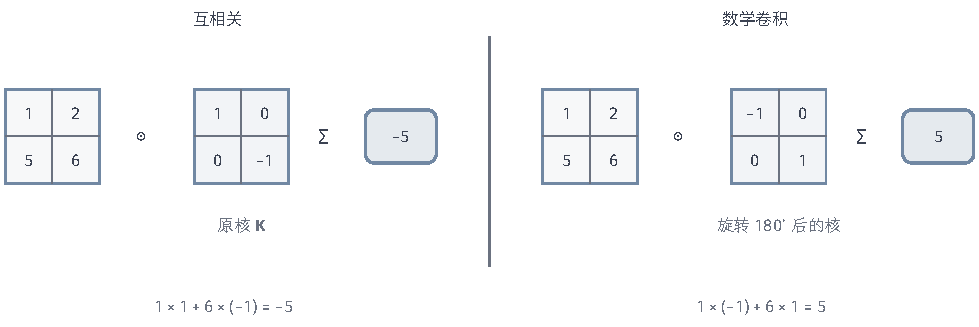
\includegraphics[width=165.767mm]{figures/03-models/02-neural-network-models/tikz/cnn-kernel-flip/figure.pdf}
  \caption{核的方向改变输出。输入窗口固定为$\left[\begin{smallmatrix}1&2\\5&6\end{smallmatrix}\right]$，核固定为$\left[\begin{smallmatrix}1&0\\0&-1\end{smallmatrix}\right]$。左侧直接逐元素相乘后求和，得到互相关输出$-5$；右侧先把核旋转$180$度，再求和，得到数学卷积输出$5$。$\odot$表示逐元素乘法，$\sum$表示把四个乘积相加。}
  \label{fig:cnn-kernel-flip}
\end{figure*}
\subsubsection{互相关：保留核的方向}
\label{sec:cnn-correlation-operation}

网络通常省去这次旋转，直接用存储的核权重对窗口求和。这种\term{互相关}（cross-correlation）是按核原有方向匹配局部输入；本章针对实数数据写为
\begin{equation}
  y_{i,j}=\sum_{a=0}^{k_h-1}\sum_{b=0}^{k_w-1}
    k_{a,b}x_{i+a,j+b}\text{。}
  \label{eq:cnn-cross-correlation}
\end{equation}
于是左上窗口得到$1-6=-5$，全部输出构成$3\times3$的常数矩阵，见图~\ref{fig:cnn-sliding-window}。对无方向约束的可学习核，翻转只是参数位置的重新排列，卷积与互相关对应同一类候选映射；对预先给定的核，方向仍会改变结果。深度学习文献和软件通常把这种互相关也称为卷积。下文的网络公式遵循这一惯例，保留“数学卷积”来指明需要翻转的运算。

\begin{figure*}[htb]
  \centering
  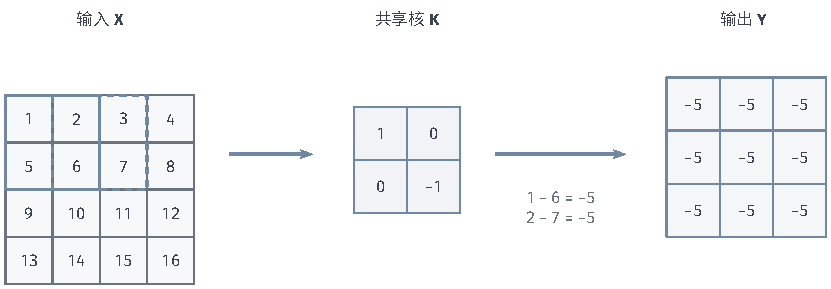
\includegraphics[width=140.723mm]{figures/03-models/02-neural-network-models/tikz/cnn-sliding-window/figure.pdf}
  \caption{共享核在二维矩阵上滑动的教学例子。蓝色实线和虚线分别框出相邻的两个$2\times2$输入窗口，中间矩阵给出保持原方向的核，右侧矩阵给出互相关输出。每个输出计算窗口左上数值减去右下数值，因此均为$-5$；两个位置使用同一组权重。}
  \label{fig:cnn-sliding-window}
\end{figure*}

\subsubsection{数据填充：确定边界假设}
\label{sec:cnn-padding-operation}

不填充时，边缘像素参与的窗口较少，输出尺寸也会缩小。\term{数据填充}（padding）在矩阵外补充数值，使核可以覆盖边缘附近的位置。零填充把外部值设为零；复制填充延续最近的边缘值；反射填充按边界镜像取值；循环填充把另一侧的数据接过来。这些外部值是由边界假设构造的，决定边缘窗口如何计算。

对式\eqref{eq:cnn-matrix-example}只在右侧和下侧各补一列、一行零，输出就有$4\times4$个位置：
\begin{equation}
  \bm Y=\begin{bmatrix}
    -5&-5&-5&4\\-5&-5&-5&8\\-5&-5&-5&12\\13&14&15&16
  \end{bmatrix}\text{。}
  \label{eq:cnn-padding-example}
\end{equation}
最后一列和最后一行改变，是因为核的负权重落到了补零区域。图~\ref{fig:cnn-padding}标出右上和右下两个窗口：相同的核在内部读取真实数值，在边界则读取约定的零。\term{valid填充}表示不添加边界值，\term{same填充}通常表示按输入尺寸和步长选择填充，使输出尺寸达到约定值。步长为一时常取输出与输入等大；偶数核可能需要不对称填充，本例就是这种情况。步长大于一时，有些接口以$\lceil h/s_h\rceil$为目标高度，具体左右分配还需核对所用约定。


\begin{figure*}[htb]
  \centering
  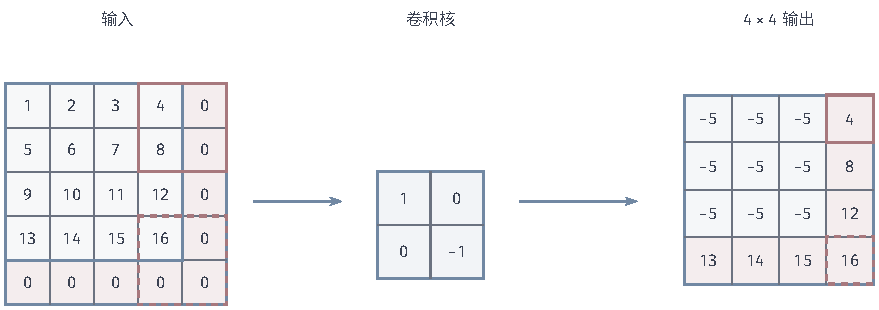
\includegraphics[width=148.791mm]{figures/03-models/02-neural-network-models/tikz/cnn-padding/figure.pdf}
  \caption{不对称零填充与边界输出。蓝色框内是原$4\times4$输入，浅红色区域是右侧、下侧各新增的一列、一行零。红色实线窗口产生右上输出$4$，虚线窗口产生右下输出$16$，输出矩阵中用相同线型标记对应位置。核为$(1,0;0,-1)$，步长一、空洞率一，计算采用互相关。}
  \label{fig:cnn-padding}
\end{figure*}
\subsubsection{跨步卷积：改变窗口移动间隔}
\label{sec:cnn-stride-operation}

填充改变可读取的位置，\term{跨步卷积}（strided convolution）则改变输出位置之间的间隔：核每次沿高、宽分别移动$s_h,s_w$个输入位置。在原例中，不填充且$s_h=s_w=2$，只保留窗口起点$(0,0),(0,2),(2,0),(2,2)$，得到$2\times2$的输出，数值仍均为$-5$。图~\ref{fig:cnn-stride}显示，减少的是窗口起点的数量，窗口内部仍读取相邻的四个元素。它同时完成局部变换与下采样；若输入包含较快的空间变化，下采样可能把不同变化混在一起，这就是采样中的混叠问题。


\begin{figure*}[htb]
  \centering
  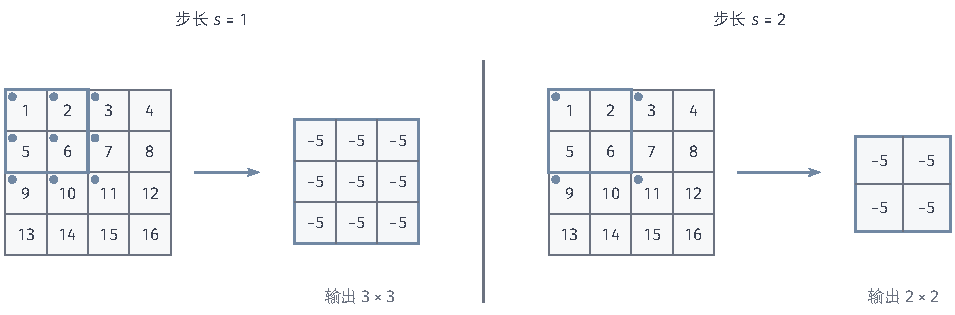
\includegraphics[width=161.766mm]{figures/03-models/02-neural-network-models/tikz/cnn-stride/figure.pdf}
  \caption{跨步改变输出位置的密度。输入、$2\times2$核和无填充设置保持不变，只将高、宽步长从一改为二。每个蓝色圆点标记一个窗口的左上起点，起点分别形成$3\times3$和$2\times2$的网格；实线框只画出第一个窗口。该教学矩阵的所有窗口都得到$-5$，输出值相同不表示读取的位置相同。}
  \label{fig:cnn-stride}
\end{figure*}
\subsubsection{空洞卷积：改变核内采样间隔}
\label{sec:cnn-dilation-operation}

若希望扩大一个输出所覆盖的区域，又不增加核参数，可以让核内部的采样点隔开。\term{空洞卷积}（dilated convolution）在相邻核元素之间跳过$d_h-1,d_w-1$个输入位置，$d_h,d_w$称为空洞率。原例取$d_h=d_w=2$、步长为一且不填充，左上输出变为$x_{0,0}-x_{2,2}=1-11=-10$，得到$2\times2$的常数输出。四个核位置覆盖$3\times3$区域，却只采样其中四点。图~\ref{fig:cnn-dilation}把权重与这些位置对应起来；图~\ref{fig:cnn-sampling}再并排区分核内采样间隔与窗口移动间隔。重复使用相同空洞率还可能留下未充分交互的网格位置，扩大覆盖范围不等于密集读取其中所有信息。


\begin{figure*}[htb]
  \centering
  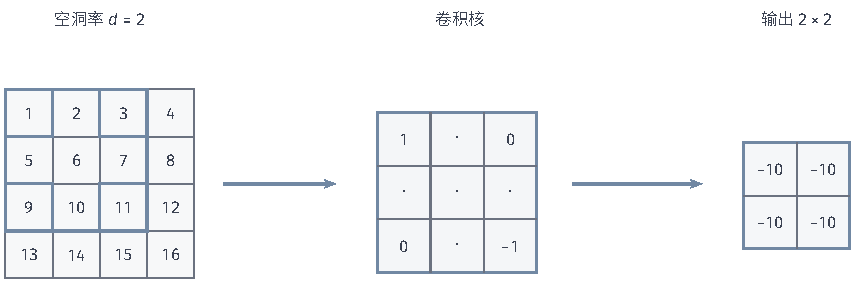
\includegraphics[width=144.766mm]{figures/03-models/02-neural-network-models/tikz/cnn-dilation/figure.pdf}
  \caption{空洞率二时的实际采样位置。左图彩色小框标出左上输出读取的四格，蓝色外框标出其$3\times3$覆盖区域；中图把原$2\times2$核权重按采样间隔排开，点号表示跳过的位置。数值零占据一个已有核位置，点号处则没有核参数。步长一、无填充时，左上输出为$1-11=-10$，全部输出构成$2\times2$矩阵。}
  \label{fig:cnn-dilation}
\end{figure*}
\subsubsection{统一表达与输出尺寸}
\label{sec:cnn-shape-operation}

把这些设置合在一起，记上下填充为$p_{\mathrm t},p_{\mathrm b}$、左右填充为$p_{\mathrm l},p_{\mathrm r}$，以$\widetilde x_{i,j}$表示在原坐标外扩展的输入值。互相关计算为
\begin{equation}
  y_{i,j}=\sum_{a=0}^{k_h-1}\sum_{b=0}^{k_w-1}
    k_{a,b}\widetilde x_{is_h-p_{\mathrm t}+ad_h,\,
                         js_w-p_{\mathrm l}+bd_w}\text{。}
  \label{eq:cnn-general-correlation}
\end{equation}
有效核尺寸为$e_h=d_h(k_h-1)+1$、$e_w=d_w(k_w-1)+1$，要求填充后的输入至少容纳一个窗口。使用只保留完整窗口的取整规则时，输出尺寸为
\begin{equation}
  \begin{aligned}
    h'&=\left\lfloor\frac{h+p_{\mathrm t}+p_{\mathrm b}-e_h}{s_h}\right\rfloor+1,\\
    w'&=\left\lfloor\frac{w+p_{\mathrm l}+p_{\mathrm r}-e_w}{s_w}\right\rfloor+1\text{。}
  \end{aligned}
  \label{eq:cnn-output-size}
\end{equation}
分子表示窗口起点可以移动的总距离，除以步长后取整得到可移动的次数，再加上起始窗口。这也解释了为什么同样的输出大小可能来自不同的输入大小：不足一个步长的尾部会被舍去。

\begin{figure*}[htb]
  \centering
  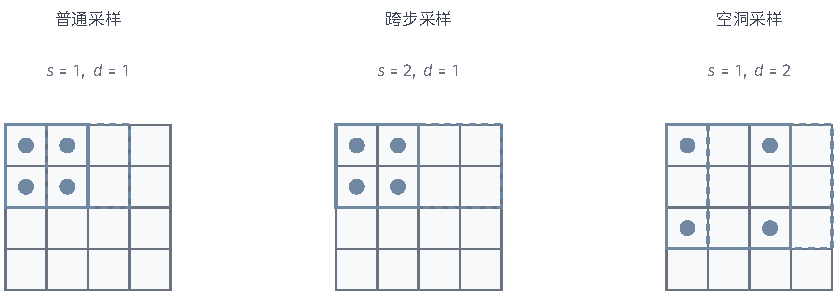
\includegraphics[width=141.792mm]{figures/03-models/02-neural-network-models/tikz/cnn-sampling/figure.pdf}
  \caption{同一个$2\times2$核的三种采样设置。实线框给出一个输出所覆盖的区域，紫点是该窗口实际读取的位置，虚线框表示下一个水平窗口。普通设置与跨步设置的核内邻距均为一，后者将窗口起点移远；空洞设置将核内邻距增为二，窗口起点仍只移动一格。}
  \label{fig:cnn-sampling}
\end{figure*}

\subsubsection{转置卷积：把局部贡献分配回去}
\label{sec:cnn-transpose-operation}

卷积也可以用矩阵表达。固定核与输入、输出形状，把输入和输出展平为$\bm x$和$\bm y$，忽略偏置，有$\bm y=\bm C\bm x$；$\bm C$每行对应一个输出，非零位置表示它读取哪些输入，共享权重在多行重复出现。\term{转置卷积}（transposed convolution）使用这个映射的转置，即对给定$\bm v$计算$\bm C^\top\bm v$，将一个输入值按核权重分配到多个输出位置，并把重叠贡献相加。

取原例第一行$(1,2,3,4)$，用一维核$(1,-1)$说明同样的过程。步长为一且不填充时，
\begin{equation}
  \bm C=\begin{bmatrix}
    1&-1&0&0\\0&1&-1&0\\0&0&1&-1
  \end{bmatrix},\qquad
  \bm C^\top\begin{bmatrix}1\\1\\1\end{bmatrix}
    =\begin{bmatrix}1\\0\\0\\-1\end{bmatrix}\text{。}
  \label{eq:cnn-transpose-example}
\end{equation}
图~\ref{fig:cnn-transpose-scatter}逐项展开分配过程。中间两个位置各收到正、负贡献，累加后成为零；转置映射的结果由这些贡献共同确定。$\bm C$把四维输入变成三维输出，已丢失某些信息；$\bm C^\top\bm C$也不等于单位矩阵。这个例子的转置映射执行了重新分配，而前向已丢失的信息仍未恢复。作为可学习层时，转置卷积也可以独立学习核参数。


\begin{figure}[htb]
  \centering
  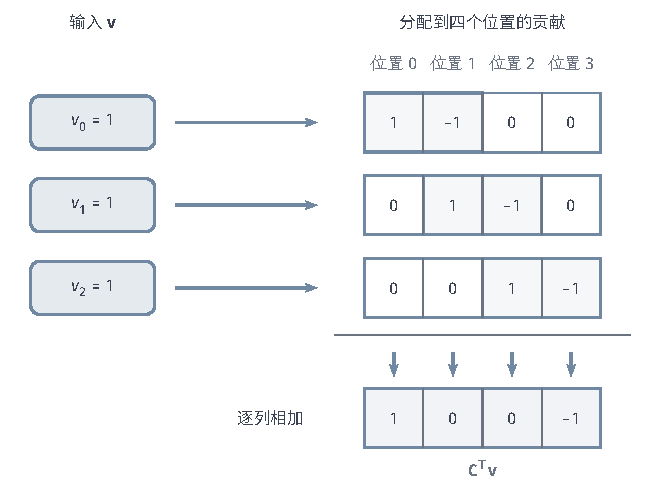
\includegraphics[width=112.000mm]{figures/03-models/02-neural-network-models/tikz/cnn-transpose-scatter/figure.pdf}
  \caption{转置卷积的分配与累加。输入为$\bm v=(1,1,1)^\top$，核为$(1,-1)$，步长一、无填充。每行分别表示一个输入值对四个输出位置的贡献，紫框圈出两个可能非零的位置；没有贡献的格子记为零。逐列相加得到$(1,0,0,-1)^\top$，中间两格均包含来自不同输入的重叠贡献。}
  \label{fig:cnn-transpose-scatter}
\end{figure}
在一维对称零填充$p$、步长$s$、空洞率$d$和核长$k$的约定下，转置卷积输入长度$n'$对应的输出长度常写为
\begin{equation}
  n_{\mathrm{out}}=(n'-1)s-2p+d(k-1)+1+o,
  \qquad 0\leq o<s\text{。}
  \label{eq:cnn-transposed-size}
\end{equation}
这里$o$是用于选择目标形状的输出填充量：普通卷积取整后，同一个$n'$可能对应$s$种原输入长度。选定目标长度后，前向矩阵的列数及其转置的输出形状才随之确定。$o$是尺寸约定，不表示把$o$个零作为最终输出值附在末尾。二维情形沿高、宽分别使用该式。不对称填充或额外裁剪会改变矩阵的边界行、列，输出形状也要随对应映射确定。跨步转置卷积可理解为先在输入位置之间插零，再进行适当的滤波与裁剪；不同位置的覆盖次数可能不均匀，需要检查输出中的周期性纹理。卷积尺寸与转置关系的系统说明见Dumoulin和Visin的算术指南\scite{dumoulin2016arithmetic}

\subsection{卷积的实现}
\label{sec:cnn-implementation}

固定边界与采样设置，在精确算术下，直接求和、矩阵化和满足适用条件的变换算法可以得到相同的预激活值。矩阵化汇集原有局部点积，Toom--Cook、Winograd与FFT通过变换输入和核来重组乘积，空间可分离路线则利用核的低秩结构（代数算法、数值例子及误差条件参考\BookSectionRef{sec:signal-analysis-fast-transforms}{第一卷“数学准备”的“卷积映射的快速计算”节}）。这里固定本层的批量、通道和采样设置，比较直接计算的成本与变换结果的复用，再说明数据如何存储和读取。

此前的单矩阵例子只保留一个数值平面，现在将第~\ref{sec:cnn-overview}节的多通道组织写成张量。一个通道在全部空间位置上的响应构成一张\term{特征图}（feature map）。单个输入的形状为$\bm X\in\mathbb R^{h\times w\times c_{\mathrm{in}}}$，普通密集卷积的核张量为$\bm W\in\mathbb R^{k_h\times k_w\times c_{\mathrm{in}}\times c_{\mathrm{out}}}$。固定一个输出通道，其核覆盖全部输入通道：对空间窗口和输入通道共同求和，产生一个输出值；换用另一组核权重便产生另一个输出通道。因此输入通道轴参与求和，输出通道轴保留在结果中，图~\ref{fig:cnn-channels}给出了对应示意。

以下比较同一个互相关映射，忽略激活；偏置可在累积完成后加入。设小批量含$n_{\mathrm b}$个输入，输入、输出通道数为$c_{\mathrm{in}},c_{\mathrm{out}}$，输出空间尺寸为$h'\times w'$。记
\[
  q=k_hk_wc_{\mathrm{in}},\qquad m=n_{\mathrm b}h'w'\text{，}
\]
即一个窗口的元素数与全部输出位置数。普通密集卷积需要$c_{\mathrm{out}}qm$次乘加；比较额外存储时，输入、核和最终输出不计入工作区。这里把输入数值与核权重相乘称为\emph{核心乘法}；在变换路线中，相应计数的是变换后输入与核的乘积。固定变换中的加减与常数乘法另外计算。总耗时还包含变换、数据读写与调度，后文据此同时计算新增的工作和存储。

矩阵化把本层的每个窗口作为一列，每个核作为一行。按一致顺序展平后，窗口矩阵为$\bm P\in\mathbb R^{q\times m}$，核矩阵为$\bm W_{\mathrm{loc}}\in\mathbb R^{c_{\mathrm{out}}\times q}$；加入偏置$\bm b\in\mathbb R^{c_{\mathrm{out}}}$后，预激活为
\begin{equation}
 \bm Z_{\mathrm{col}}=\bm W_{\mathrm{loc}}\bm P+\bm b\bm1_m^\top.
 \label{eq:cnn-im2col}
\end{equation}
其中$\bm1_m$是$m$维全一向量。这个矩阵等式把同一组局部点积汇集为\term{通用矩阵乘法}（general matrix multiplication, GEMM）；按普通矩阵乘法逐项求和时，乘加量仍与直接计算相同。

\subsubsection{直接计算：逐项求和}
\label{sec:cnn-direct-implementation}

直接算法在每个输出位置逐项累积窗口中的贡献。将批量索引记为$t$，输入元素为$x_{t,i,j,c}$，$w_{a,b,c,o}$表示核位置$(a,b)$上从输入通道$c$到输出通道$o$的权重。记$u(i,a)=is_h-p_{\mathrm t}+ad_h$、$v(j,b)=js_w-p_{\mathrm l}+bd_w$，即式\eqref{eq:cnn-general-correlation}中的实际读取位置，零填充下的核心步骤如下。
\Needspace{13\baselineskip}
\begin{algorithm}[直接多通道互相关]
  \label{alg:cnn-direct}
  \begin{algorithmic}[1]
    \Require 输入$\bm X$、核$\bm W$、偏置$\bm b$及形状、采样设置
    \Ensure 输出预激活$\bm Z$
    \For{每个合法的$(t,i,j,o)$}
      \State $z_{t,i,j,o}\gets b_o$
      \For{每个核位置$(a,b)$和输入通道$c$}
        \State 读取扩展输入$\widetilde x_{t,u(i,a),v(j,b),c}$
        \State $z_{t,i,j,o}\gets z_{t,i,j,o}+w_{a,b,c,o}\widetilde x_{t,u(i,a),v(j,b),c}$
      \EndFor
    \EndFor
  \end{algorithmic}
\end{algorithm}

算法\ref{alg:cnn-direct}的一次外层迭代只负责一个输出。核位置确定空间偏移，输入通道决定读取哪个数值，输出通道决定使用哪组权重；所有贡献加到同一个累积器中，完成后才写出。相邻输出重新使用核，另一个输出通道则使用另一个核，但二者都从同一输入张量取数。

对式\eqref{eq:cnn-matrix-example}的左上输出，顺序计算的四项是$1\times1$、$2\times0$、$5\times0$和$6\times(-1)$，总和为$-5$。零权重是这个例子的特殊取值，普通密集算法仍按四个位置组织计算；只有专门利用零权重结构，才能省去相应乘法。每个窗口含$q$项，一共有$c_{\mathrm{out}}m$个输出，因此乘加量为
\begin{equation}
  O\!\left(n_{\mathrm b}h'w'c_{\mathrm{in}}c_{\mathrm{out}}k_hk_w\right)\text{。}
  \label{eq:cnn-direct-cost}
\end{equation}
直接算法逐项保留局部求和结构，额外工作区可以只包含若干累积器，但算术量随核面积、通道数与输出位置数相乘。相邻窗口存在重叠时，共用输入可以在较近的存储中复用；这种复用属于第~\ref{sec:cnn-engineering}节的数据调度问题。判断一种计算算法时，应先固定数学运算及其乘加量，再考察它在具体存储层次中的执行方式。

\subsubsection{多通道卷积的变换复用}
\label{sec:cnn-transform-reuse}

本层的多个输出通道读取相同的窗口，同一个核又作用于多个位置。这两种共享关系使输入变换能跨输出通道复用，核变换能跨位置复用。
以步长一、无空洞的$3\times3$核为例，Winograd方案用固定矩阵$\bm B^\top,\bm G,\bm A^\top$分别变换输入、变换核并恢复输出，将一个$4\times4$输入块变为$2\times2$输出。其中输入变换矩阵为四行四列，核变换矩阵为四行三列，输出恢复矩阵为两行四列（变换矩阵及恢复等式参考\BookSectionRef{sec:signal-analysis-fast-winograd}{第一卷“数学准备”的“基于余数分解的卷积计算”小节}）。
固定一个样本的输入块，对输入通道$c$和输出通道$o$，分别形成核变换$\bm U_{c,o}=\bm G\bm W_{c,o}\bm G^\top$与输入变换$\bm V_c=\bm B^\top\bm X_c\bm B$。其中$\bm W_{c,o}\in\mathbb R^{3\times3}$是核在通道$(c,o)$上的空间切片，$\bm X_c\in\mathbb R^{4\times4}$是该输入块在通道$c$上的空间切片。
通道累积与输出恢复写成
\begin{equation}
 \bm Y_o=\bm A^\top\left(\sum_c\bm U_{c,o}\odot\bm V_c\right)\bm A.
 \label{eq:cnn-winograd-channel-reuse}
\end{equation}
式中的乘积按对应位置逐元素相乘，再对全部输入通道求和。输入变换可供多个输出通道复用，核变换可供多个空间块与批量样本复用。
由于输出变换是线性的，先对通道求和再恢复，与逐通道恢复后相加等价，却只需为每个输出通道执行一次恢复。
若同时处理$n_{\mathrm{tile}}$个输入块，在每个变换位置上还可把核组合排成$c_{\mathrm{out}}\times c_{\mathrm{in}}$矩阵，输入组合排成$c_{\mathrm{in}}\times n_{\mathrm{tile}}$矩阵。
这一$F(2\times2,3\times3)$方案的记号依次表示输出块和核的空间尺寸。其变换结果可以组织为十六组通道矩阵乘法，与GEMM组合使用。

实现时将输出切为不重叠的$2\times2$块，各自读取$4\times4$输入块，再恢复四个空间输出并加偏置。
相邻输出块起点相隔两格，输入块重叠两行或两列；边缘不足一块时需要填充或单独处理。
变换核保存十六个系数，而原核只有九个系数，活动值工作区也会扩大；分块可以限制同时保存的变换值。
更大的输出块通常还会增加变换成本和数值敏感性，步长与空洞率改变后也不能直接沿用这些矩阵。

频域路线有相同的通道共享关系。对适当翻转并补零后的核，每个频率上的输出为$\widehat y_o=\sum_c\widehat x_c\widehat k_{c,o}$，随后对各输出通道反变换，并按本层规则裁剪和选取输出位置。
若补零后的二维网格含$N$个位置，核心频域乘加量为$O(n_{\mathrm b}c_{\mathrm{in}}c_{\mathrm{out}}N)$；输入、核和输出的变换成本分别为
\begin{align*}
 \text{输入变换：}\quad &O(n_{\mathrm b}c_{\mathrm{in}}N\log N),\\
 \text{核变换：}\quad &O(c_{\mathrm{in}}c_{\mathrm{out}}N\log N),\\
 \text{输出变换：}\quad &O(n_{\mathrm b}c_{\mathrm{out}}N\log N).
\end{align*}
这里$N$是二维网格的总位置数，复数乘法也不能按一次实数乘法计价。
输入频谱可供多个输出核复用，核频谱在参数不变时可跨样本复用；训练更新参数后需要重算。
Mathieu等研究了在CNN中利用这些复用关系的FFT实现\scite{mathieu2014fft}

将单个空间核分解为若干秩一核，可把二维滤波组织为若干组一维滤波，再将结果求和（分解与计算成本参考\BookSectionRef{sec:signal-analysis-fast-separable}{第一卷“数学准备”的“基于核分离的卷积计算”小节}）。保留全部非零秩一项时，在相同边界和采样约定下恢复原来的空间核；计算能否减少，还取决于核的秩、输入尺寸与边界处理成本。截断分解会改变本层输出，需要检查近似误差或重新训练。第~\ref{sec:cnn-layer}节的深度可分离卷积则改变通道连接方式，以逐通道空间滤波和逐点通道混合两步构造新的参数结构。

\subsubsection{工程实现与优化}
\label{sec:cnn-engineering}

计算算法确定需要哪些乘积与求和，执行速度还取决于数据如何送入计算单元。\term{分块}（tiling）把相邻输出位置和若干通道放在一起计算，在较近的存储中复用它们共用的输入与核，减少重复读取。块越大，复用机会越多，但寄存器和局部存储需求也越高，可能限制并行度。

矩阵化卷积需要决定如何提供式\eqref{eq:cnn-im2col}中的窗口矩阵。\term{数据展开}（im2col）把窗口复制为连续的列，再调用GEMM；显式保存整个矩阵需要$qm$个元素，还会产生展开读写。\term{隐式GEMM}（implicit GEMM）则从原张量按需形成当前计算块所需的片段，省去完整展开矩阵，代价是加载时的地址计算与边界判断。CUTLASS给出了这种实现方式\scite{nvidiaCutlassConvolution}

另一种选择是\term{间接卷积}（indirect convolution）：保存指向原输入通道向量的地址，由专用内核沿地址取数，避免复制全部窗口数值。它与隐式GEMM的区别在于显式记录取数位置，也需要承担地址表和间接访存的成本；沿地址取数需要专门的执行内核，普通GEMM接收的则是数值矩阵\scite{dukhan2019indirect}

卷积之后的偏置和逐元素激活还可在写出前完成，这种\term{算子融合}（operator fusion）减少中间结果的读写与调用次数。分块、布局和融合可用于不同算法，但收益取决于层形状、精度、硬件及训练或推理条件。完整算子的时间、工作区与数值误差，反映了乘法节省与新增成本的合计结果。存储层次、并行调度与融合的具体实现留到
\BookVolumeRef{vol:systems}{第六卷}“系统”展开。

\FloatBarrier

\section{网络结构}
\label{sec:cnn-structure}

一次局部求和只能产生一组线性响应。完整网络还需要用多个核形成不同特征，用非线性组合这些特征，按任务保留或汇聚位置，并把最终结果转换为可比较的预测。以下分别说明这些层的读取、汇聚和输出作用，再组合成完整架构。

\subsection{卷积层}
\label{sec:cnn-layer}

沿用第~\ref{sec:cnn-implementation}节的输入与核张量形状，加入偏置$\bm b\in\mathbb R^{c_{\mathrm{out}}}$。空间和核索引从零开始，通道索引$c,o$从一开始；$x_{i,j,c}$、$w_{a,b,c,o}$、$b_o$分别是输入、核与偏置的元素。输出预激活值$\bm Z\in\mathbb R^{h'\times w'\times c_{\mathrm{out}}}$为
\begin{equation}
  \begin{aligned}
    z_{i,j,o}=b_o+\sum_{c=1}^{c_{\mathrm{in}}}
      \sum_{a=0}^{k_h-1}\sum_{b=0}^{k_w-1}
      w_{a,b,c,o}\widetilde x_{u(i,a),v(j,b),c},\\
    u(i,a)=is_h-p_{\mathrm t}+ad_h,\qquad
    v(j,b)=js_w-p_{\mathrm l}+bd_w\text{。}
  \end{aligned}
  \label{eq:cnn-layer-forward}
\end{equation}
随后通常逐元素应用激活，得到$h_{i,j,o}=\sigma(z_{i,j,o})$。图~\ref{fig:cnn-channels}把式中的通道求和展开，展示同一组输入怎样形成多个输出通道。

\begin{figure*}[htb]
  \centering
  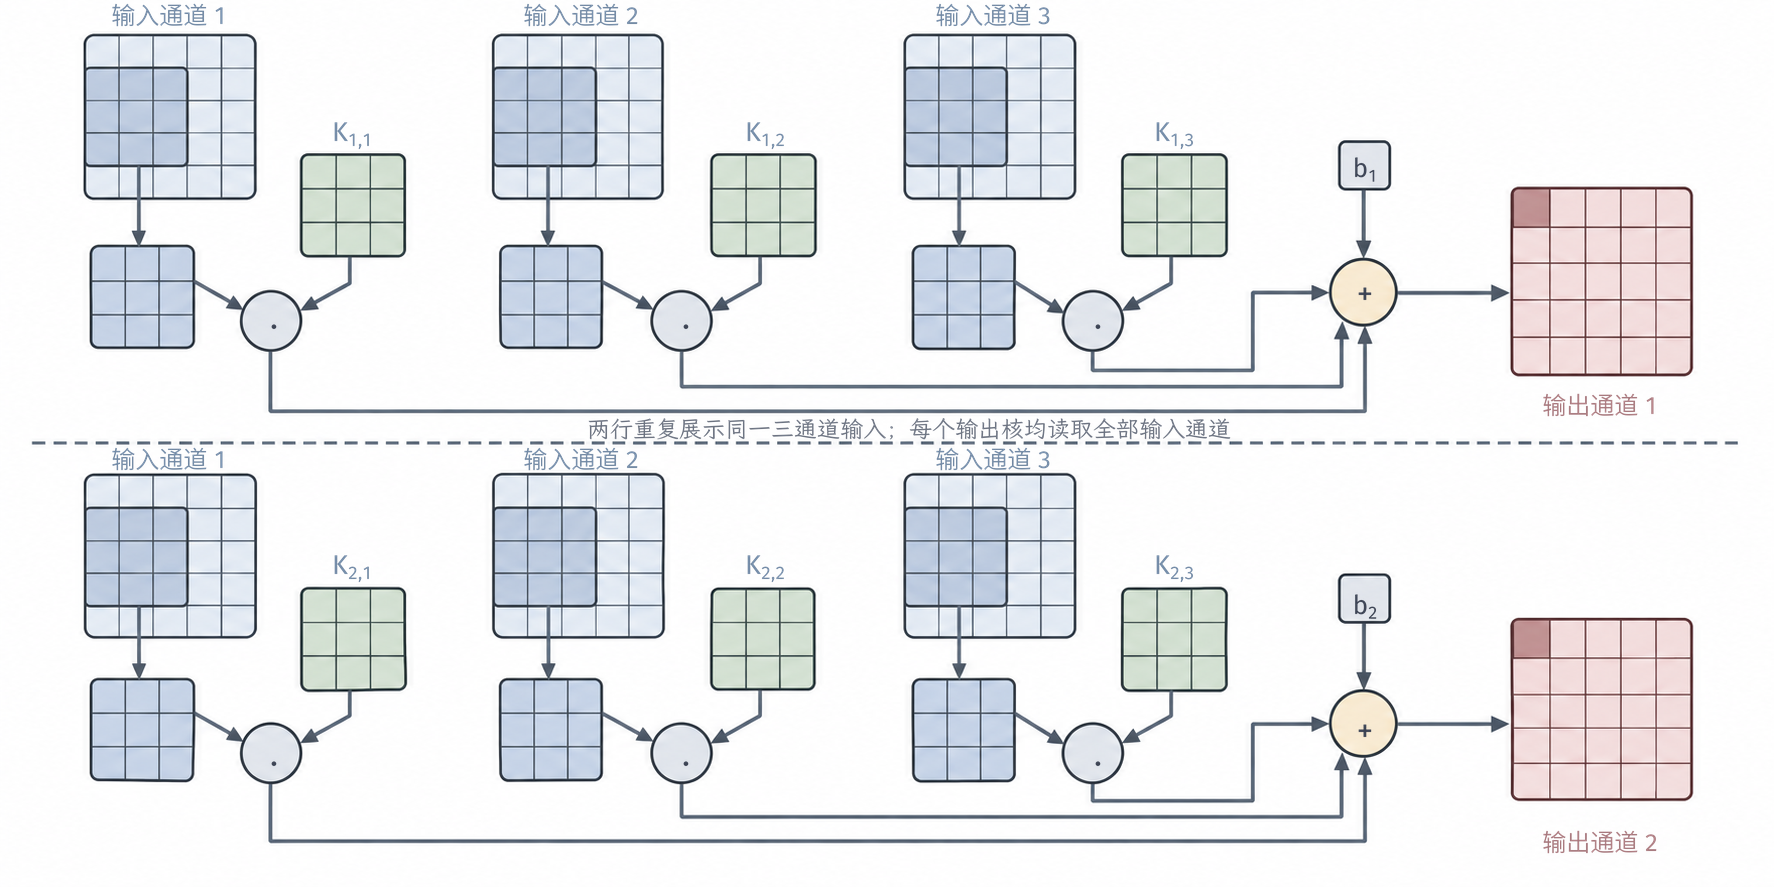
\includegraphics[width=150.199mm]{figures/03-models/02-neural-network-models/generated/cnn-channels/figure.png}
  \caption{三输入、两输出通道的卷积。每行展示同一输入张量$\bm X$的三个通道；一组输出核包含三个通道切片，各自读取对应输入通道中高亮的局部窗口。各切片完成局部乘加后，三项贡献与偏置一起求和，分别写入右侧输出张量$\bm Z$的两个通道；两个输出平面分别由核1、核2产生。网格只示意通道与局部窗口的关系，不声明实际空间尺寸、步长或填充；核在空间位置间共享，输出尺寸由正文公式确定。}
  \label{fig:cnn-channels}
\end{figure*}

普通卷积层的参数数为
\begin{equation}
  p_{\mathrm{conv}}=k_hk_wc_{\mathrm{in}}c_{\mathrm{out}}
                    +c_{\mathrm{out}}\text{。}
  \label{eq:cnn-layer-parameters}
\end{equation}
空间尺寸没有出现在该式中，却仍出现在式\eqref{eq:cnn-direct-cost}的计算量和活动值存储量中。较大图像可以使用相同参数，但要生成更多响应。因此参数量由核形状决定，计算量和活动值内存还随空间网格扩大。

核为$1\times1$时，每个输出只读取同一空间位置的通道向量。\term{逐点卷积}（pointwise convolution）因此是所有位置共享的通道变换，可以增加、压缩或混合通道，却不直接扩展空间感受野。\term{分组卷积}（grouped convolution）把输入、输出通道分成$g$组，各组只在内部连接；若两类通道数都能被$g$整除，权重数变为$k_hk_wc_{\mathrm{in}}c_{\mathrm{out}}/g$。若每个输入通道单独使用一个空间核，再接逐点卷积混合通道，就得到一种\term{深度可分离卷积}（depthwise separable convolution）：将空间处理与通道混合分成两步。在每个输入通道产生一张中间图的设置下，权重数为$k_hk_wc_{\mathrm{in}}+c_{\mathrm{in}}c_{\mathrm{out}}$，但两步施加的结构约束也与普通卷积不同。

图~\ref{fig:cnn-channel-connectivity-comparison}固定四个输入与四个输出通道，比较通道连接的改变。三个配置采用相同空间核，但读取的通道集合不同；深度可分离配置还通过后续逐点变换建立跨通道交互。

\begin{figure*}[htbp]
  \centering
  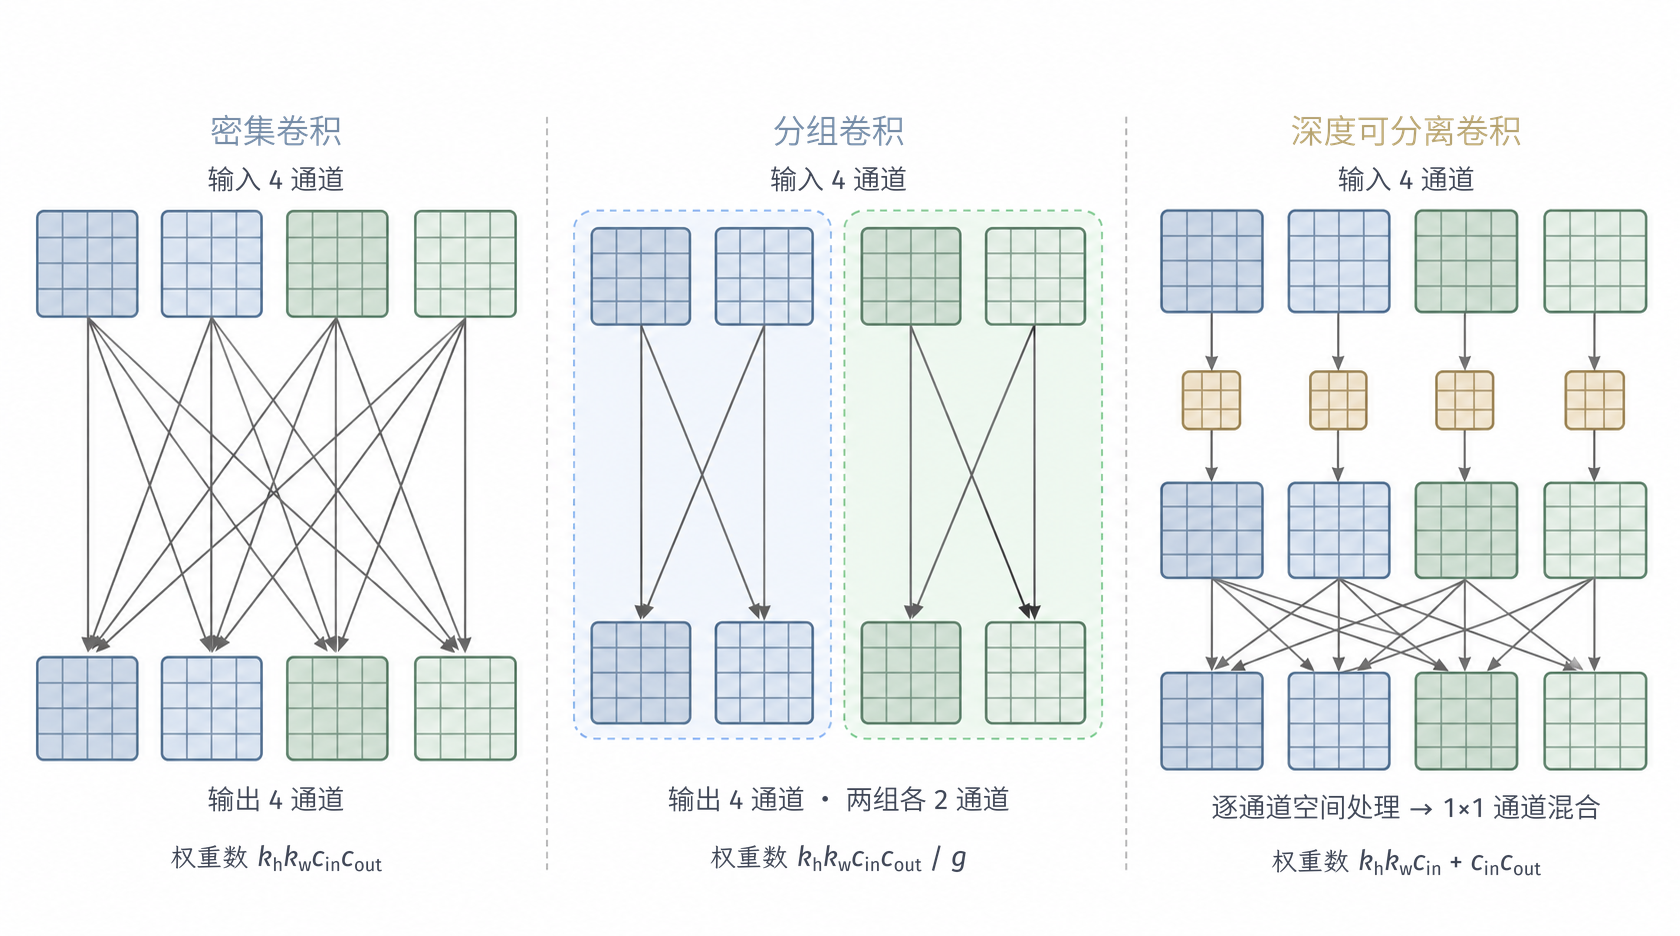
\includegraphics[width=142.240mm]{figures/03-models/02-neural-network-models/generated/cnn-channel-connectivity-comparison/figure.png}
  \caption{四输入、四输出通道上的三种连接。密集卷积读取所有输入通道；两组卷积仅在各组内部连接；深度可分离卷积先逐通道完成空间处理，再用$1\times1$卷积混合通道。权重数忽略偏置，分组数为二，深度乘子为一。}
  \label{fig:cnn-channel-connectivity-comparison}
\end{figure*}

多层组合让一个高层单元读取更大的输入范围。沿由局部卷积、局部池化和逐点运算组成的单条串联路径，设第$\ell$层的有效核尺寸为$e_\ell$、步长为$s_\ell$，$r_\ell$表示感受野跨度，$j_\ell$表示相邻响应在原输入上的间距。对一个轴，有
\begin{equation}
  r_0=j_0=1,\qquad
  r_\ell=r_{\ell-1}+(e_\ell-1)j_{\ell-1},\qquad
  j_\ell=s_\ell j_{\ell-1}\text{。}
  \label{eq:cnn-receptive-field}
\end{equation}
新增的$e_\ell-1$个间隔，每个在原输入上跨越$j_{\ell-1}$个位置，所以要相乘。以两个空洞率一、步长一的$3\times3$层为例，沿任一轴代入$e_1=e_2=3$和$s_1=s_2=1$，得到
\[
  \begin{aligned}
    r_1&=1+(3-1)\times1=3,& j_1&=1\times1=1,\\
    r_2&=3+(3-1)\times1=5,& j_2&=1\times1=1\text{。}
  \end{aligned}
\]
第二层读取三个相邻的第一层响应，它们各覆盖三个原输入位置，覆盖范围每次只平移一个位置，因此合起来是五个位置，而非九个。高、宽两轴分别计算，便得到$5\times5$；再接同样的一层则为$7\times7$。

若只把第一层的步长改为二，仍有$r_1=3$，但$j_1=2\times1=2$，第二层于是得到$r_2=3+(3-1)\times2=7$、$j_2=1\times2=2$。这里第二层窗口内的相邻响应在原输入上相隔两个位置，故覆盖$7\times7$。一般地，$j_{\ell-1}=\prod_{a=1}^{\ell-1}s_a$是此前各层步长的乘积，空乘积取一；它把当前层的间隔换算回原输入尺度。

这是忽略跨空间统计等非局部操作后的几何感受野；实际梯度和学到的权重可能集中在其中一部分，空洞采样也可能使范围内存在未读取的位置。含归一化的网络还需计入统计量带来的额外依赖，见第~\ref{sec:cnn-activation-normalization}节。填充决定响应中心对应哪个输入位置，边界响应的实际读取范围还会被原图尺寸截断。

\FloatBarrier

\subsection{池化层}
\label{sec:cnn-pooling}

某个局部区域内出现了一个特征时，后续计算有时只需要其强度，不需要每个位置的响应。\term{池化}（pooling）按预设规则汇聚窗口内的数值，通常对每个通道独立作用。它与卷积都读取窗口，但标准池化不学习窗口中的权重，也不直接混合通道。

设输出位置$(i,j)$在某通道读取的非空有效输入位置集合为$\Omega_{i,j}$，其元素个数为$q_{i,j}$。\term{最大池化}（max pooling）保留窗口内的最大响应，\term{平均池化}（average pooling）保留窗口内的平均响应：
\begin{equation}
  \begin{aligned}
    y_{i,j,c}^{\mathrm{max}}&=\max_{(u,v)\in\Omega_{i,j}}x_{u,v,c},\\
    y_{i,j,c}^{\mathrm{avg}}&=\frac1{q_{i,j}}
                   \sum_{(u,v)\in\Omega_{i,j}}x_{u,v,c}\text{。}
  \end{aligned}
  \label{eq:cnn-local-pooling}
\end{equation}
在式\eqref{eq:cnn-matrix-example}上用不重叠的$2\times2$窗口、步长二且不填充，分别得到
\begin{equation}
  \bm Y^{\mathrm{max}}=\begin{bmatrix}6&8\\14&16\end{bmatrix},\qquad
  \bm Y^{\mathrm{avg}}=\begin{bmatrix}3.5&5.5\\11.5&13.5\end{bmatrix}\text{。}
  \label{eq:cnn-pooling-example}
\end{equation}
最大池化侧重最强响应，平均池化反映整体水平。两者都丢失窗口内的部分信息：仅凭$6$不能知道该窗口的其他三个值，仅凭$3.5$也不能知道四个值的排列。

采用相同窗口与完整窗口取整规则时，池化的输出尺寸可由式\eqref{eq:cnn-output-size}计算。边界规则却要单独核对：最大池化常将无效位置排除，等价于用负无穷填充，而补零会改变全负窗口的最大值；平均池化若把补零位置计入分母，边缘均值会与只除以有效元素数不同。使用向上取整的接口还会保留末尾窗口，并对其边界另作处理；这会给出与本章向下取整约定不同的形状。

\term{全局平均池化}（global average pooling）把每张特征图汇成一个数，得到通道向量$\bm r\in\mathbb R^{c_{\mathrm{in}}}$：
\begin{equation}
  r_c=\frac1{hw}\sum_{i=0}^{h-1}\sum_{j=0}^{w-1}x_{i,j,c}\text{。}
  \label{eq:cnn-global-average-pooling}
\end{equation}
全局最大池化则保留每个通道在全部位置上的最大值。若平移仅对特征图作位置置换，例如循环边界上的整数平移，这两种汇聚都保持结果不变。实际网络中的填充、裁剪和跨步可能改变平移后的特征值和采样位置，此时上述置换条件不再成立。局部池化保留的是窗口中的最大值或平均值，其平移性质也由窗口如何移动决定。

\subsection{激活与归一化}
\label{sec:cnn-activation-normalization}

卷积层仍然是仿射映射，单独堆叠不足以学习复杂的非线性关系。ReLU、GELU或SiLU可逐元素作用于特征图，保留空间和通道形状，同时改变局部响应。它们的定义、梯度和初始化配合见第~\ref{sec:ffn-activations}节。这些隐藏层激活决定局部特征如何组合；末端的概率或取值范围，则由输出任务另行规定。

深层组合还会改变活动值的尺度。\term{批归一化}（batch normalization, BN）用当前小批量的统计量调整特征，再学习一个缩放与平移。对卷积特征，通常按通道在批量轴和两个空间轴上统计；设小批量预激活为$z_{t,i,j,c}$、样本索引$t=1,\ldots,n_{\mathrm b}$，统计元素数为$m=n_{\mathrm b}h'w'$，则
\begin{equation}
  \begin{aligned}
    \mu_c&=\frac1m\sum_{t,i,j}z_{t,i,j,c},\qquad
    v_c=\frac1m\sum_{t,i,j}(z_{t,i,j,c}-\mu_c)^2,\\
    \widehat z_{t,i,j,c}&=\frac{z_{t,i,j,c}-\mu_c}{\sqrt{v_c+\epsilon}},\qquad
    \bar z_{t,i,j,c}=\gamma_c\widehat z_{t,i,j,c}+\beta_c\text{。}
  \end{aligned}
  \label{eq:cnn-batch-normalization}
\end{equation}
其中$\epsilon>0$防止分母过小。固定通道$c$后，均值与方差汇集全部$n_{\mathrm b}h'w'$个数值，不跨通道求和；同一组可学习参数$\gamma_c,\beta_c$也在这些样本和空间位置之间共享，不为每个像素位置另设一组参数。

全连接前馈网络的BN使用相同原则，但没有空间轴。将一个小批量的特征按行排成$\bm Z_{\mathrm{FFN}}\in\mathbb R^{n_{\mathrm b}\times d}$，固定特征坐标$q$，就只在$\{z_{t,q}:t=1,\ldots,n_{\mathrm b}\}$上统计均值与方差，$\gamma_q,\beta_q$在样本间共享。因此，FFN的“特征级”BN固定一列、跨样本统计，CNN的“通道级”BN固定一个通道、跨样本和空间位置统计。若把卷积特征展平成$n_{\mathrm b}\times(h'w'c_{\mathrm{out}})$后逐列做BN，每个空间位置会分别统计并拥有各自的仿射参数，这与卷积BN不同。其他归一化方法的统计轴对照见图~\ref{fig:training-normalization-axes}。

训练时，共用均值与方差使这些数值的计算相互耦合：一个值改变，可能影响同组其他值的归一化结果。CNN的这种依赖既跨样本，也跨同一通道的空间位置。推理时通常使用训练中累计的均值与方差，使单样本计算固定。累计统计量按实现选定的估计规则更新。常见组合是“卷积—BN—ReLU”，紧接BN的卷积偏置常可省略，因为通道中心化会消除它，BN另有平移参数\scite{ioffe2015batchnorm}

当批量较小或批内组成变化较大时，可以改变统计范围。\term{组归一化}（group normalization, GN）把通道分成若干组，对每个样本分别在一组通道及其空间位置上统计均值和方差，然后仍按通道学习缩放与平移。它不需要其他样本提供统计量，训练和推理使用相同的统计范围，但会让同组通道发生统计耦合。组数是结构设置，通道数需要能够均分。GN与BN的区别首先在统计对象：前者独立处理样本，后者使用批内信息。实际训练效果还随任务和批量设置变化\scite{wu2018groupnorm}

这些统计量也改变数据依赖范围。训练态BN通过通道均值与方差连接同批样本的不同空间位置，GN则在训练和推理时都连接同一样本组内的各空间位置；式\eqref{eq:cnn-receptive-field}没有计入这些路径。推理态BN若使用固定的运行统计量，就只是逐点仿射变换，不会额外扩大依赖范围。

归一化、激活和池化的顺序影响计算含义。对平均池化，通常有$\sigma(\operatorname{Avg}(\bm X))\neq\operatorname{Avg}(\sigma(\bm X))$；例如两个响应为$-2$和$1$时，先平均再ReLU得到$0$，先ReLU再平均得到$1/2$。单调逐点激活与不含额外填充值的最大池化可以交换；归一化还读取组内统计量，改变顺序就可能改变输出。各架构因而用明确的模块顺序确定计算；跨架构的训练机制由后续《神经网络的训练》章展开。

\subsection{输出和学习目标}
\label{sec:cnn-output-objectives}

预测整张图像的类别时，需要把空间特征转换为整体得分。可以将末层特征展平后接全连接层，也可以先作全局平均池化再接分类层。设汇聚向量为$\bm r$，类别数为$q$，原始得分为$\bm a=\bm U\bm r+\bm d\in\mathbb R^q$，则多类概率与单样本损失为
\begin{equation}
  p_k=\frac{\exp(a_k)}{\sum_{v=1}^{q}\exp(a_v)},\qquad
  \ell=-\log p_y\text{。}
  \label{eq:cnn-image-classification}
\end{equation}
这里$y\in\{1,\ldots,q\}$为图像标签；训练学习卷积特征与分类层参数，使用时取最大得分类别。回归、二分类和多标签输出可以沿用第~\ref{sec:ffn-output-objectives}节的变换与损失。分类输出的概率由这组类别得分共同归一化，最后一张特征图的数值本身仍是内部响应。

若要预测每个像素的类别，就需要保留或恢复空间轴。设得分张量为$\bm A\in\mathbb R^{h\times w\times q}$，在每个位置单独应用Softmax，可得到$p_{i,j,k}$。给定像素标签$y_{i,j}$，逐位置交叉熵为
\begin{equation}
  \ell_{\mathrm{seg}}=-\frac1{|\Omega|}
    \sum_{(i,j)\in\Omega}\log p_{i,j,y_{i,j}}\text{。}
  \label{eq:cnn-segmentation-loss}
\end{equation}
其中$\Omega$为非空的有标签位置集合，未标注像素不参与求和。每个位置输出多个颜色值或其他连续量时，可改用回归损失。两种输出任务都用卷积特征，却对空间汇聚有不同要求：分类可以舍去具体位置，分割和图像生成必须保留输出与位置之间的对应。

对$n$个独立训练样本，用$\bm\theta$收集所有可学习核、偏置、归一化参数和输出层参数。若网络不含跨样本操作，前向映射可逐样本计算，经验目标可写为
\begin{equation}
  \widehat R_S(\bm\theta)=\frac1n\sum_{t=1}^{n}
    \ell\!\left(\bm f_{\bm\theta}(\bm X_t),\bm Y_t\right)\text{。}
  \label{eq:cnn-training-objective}
\end{equation}
这里$\bm Y_t$统指与任务对应的目标；标量类别标签按式\eqref{eq:cnn-image-classification}处理。像素损失可在单张图像内部先汇聚，再在图像之间取平均。

使用固定统计量的推理态BN符合上述逐样本前向条件，训练态BN则不符合。给定非空批索引集$B$，将整批输入记为$\bm X_B=(\bm X_t)_{t\in B}$，用$\bm F_{\bm\theta}(\bm X_B)_t$表示批预测中对应样本$t$的输出。一次更新所用的数据损失为
\begin{equation}
  L_B(\bm\theta)=\frac1{|B|}\sum_{t\in B}
    \ell\!\left(\bm F_{\bm\theta}(\bm X_B)_t,\bm Y_t\right)\text{。}
  \label{eq:cnn-batch-objective}
\end{equation}
各项损失仍可相加，但每项预测都可能依赖整批输入。求导沿完整批计算图回传，包括均值与方差连接不同样本的路径。分别运行单样本前向会改变归一化统计量及其导数，求导后再平均得到的量一般不同于$\nabla_{\bm\theta}L_B$。若要定义随机分批训练的总体目标，还需给定批抽样规则，再对$L_B$取期望；梯度累积与一次大批前向的区别见第~\ref{sec:training-inexact-gradients}节。正则项、数据增强和优化策略可以加入训练过程，本章重点是结构特有的梯度与信息传递。

\FloatBarrier

\subsection{常见卷积网络架构}
\label{sec:cnn-classic-architectures}

完整架构要在空间精度、特征种类和计算成本之间分配资源。下采样减少空间位置，高层增加通道可以在较粗网格上保存更多特征；末端再根据任务读出。LeNet、AlexNet、VGG和GoogLeNet分别体现了局部到整体、容量扩大、规则小核和多尺度分支的组织方式。图中叠片表示特征张量，正面示意空间网格，叠片示意通道维；深色局部块与算子内部的虚线突出一次局部映射。下方细节用层名对应主链中的算子，独立展示局部计算。全连接层用包含圆形神经元的平面方框表示。蓝色用于卷积特征与全连接，黄色用于池化或降采样，绿色用于少量卷积核细节。主路径从左向右展开，实际尺寸写在各层或阶段下方；绘图尺寸不与张量元素数严格成比例。

\subsubsection{LeNet-5：从局部检测到整体读出}
\label{sec:cnn-lenet}

手写字符的局部笔画需要逐渐组合成整字。LeNet-5交替使用卷积与降采样，先形成小范围响应，再扩大后层能够读取的区域。原网络接收$32\times32$的单通道图像，C1用六个$5\times5$核产生$28\times28\times6$特征；S2降为$14\times14\times6$，C3产生$10\times10\times16$，S4再降为$5\times5\times16$。C5用覆盖整个$5\times5$区域的核得到120个整体特征，接84单元的F6，再计算十类输出，见图~\ref{fig:cnn-lenet}\scite{lecun1998}

\begin{figure*}[tbp]
  \centering
  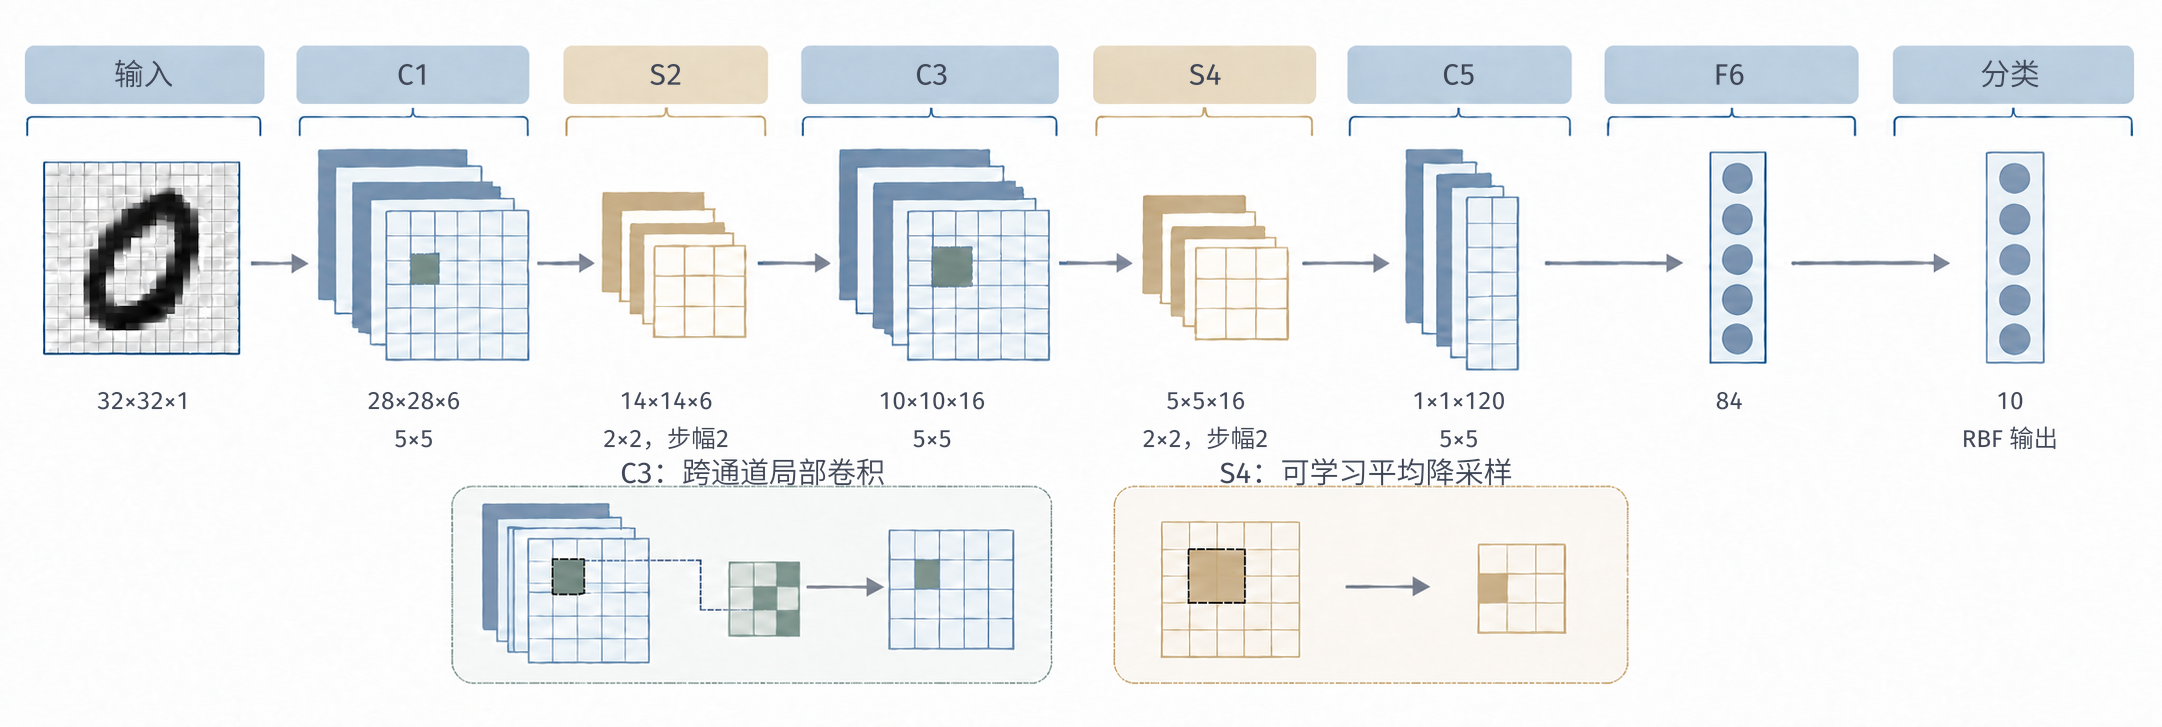
\includegraphics[width=169.000mm]{figures/03-models/02-neural-network-models/generated/cnn-lenet/figure.png}
  \caption{LeNet-5的层次结构。特征张量用叠片表示，层名与空间、通道尺寸标注在对应图元附近。C1、C3、C5为卷积层，S2、S4为可学习的平均降采样层，F6含84个单元，原始十类读出采用欧氏径向基函数。下方分别展开C3的跨通道局部卷积和S4的平均降采样；网格、叠片数和节点数均为示意，尺寸标签给出真实形状，C3部分通道连接未逐条展开。}
  \label{fig:cnn-lenet}
\end{figure*}

S2和S4采用可学习的降采样：每张特征图的局部求和还经过可学习缩放、偏置和非线性。C3采用指定的部分通道连接，不同输出读取不同的输入组合。C5虽然空间输出为$1\times1$，仍是卷积层；对这里固定的输入形状，它恰好具有整体连接的作用。

教学中常见的“普通卷积—平均池化—ReLU—Softmax”版本使用现代算子重写了这条处理链。它仍按局部检测、空间缩小和整体读出组织计算，但降采样参数、通道连接和输出规则已改变。具体版本由这些计算约定共同确定。

\FloatBarrier

\subsubsection{AlexNet：扩大容量并组织GPU训练}
\label{sec:cnn-alexnet}

自然图像包含更多颜色、纹理和尺度变化，需要更丰富的局部表示。AlexNet包含五个卷积层和三个全连接层；隐藏层使用ReLU，在第一、第二和第五个卷积阶段后作最大池化，在前两个全连接层使用Dropout。卷积主体输出通道依次为$96,256,384,384,256$，前两层分别用较大核快速扩大覆盖范围，后三层用$3\times3$继续组合特征\scite{krizhevsky2012}

图~\ref{fig:cnn-alexnet}采用能明确核算形状的$227\times227$教学输入约定。所有卷积不使用空洞，卷积与池化的空间尺寸均按式\eqref{eq:cnn-output-size}向下取整；三次最大池化均为$3\times3$窗口、步长二、无填充。首层卷积以$11\times11$核、步长四、无填充产生$55\times55$输出，池化降到$27\times27$；第二卷积使用$5\times5$核、步长一、四周各填充二，保持尺度，池化降到$13\times13$；后三层均为$3\times3$核、步长一、四周各填充一，保持该尺度。末次池化形成$6\times6\times256$，展平为9216维，接4096、4096和1000单元。原论文正文写输入$224\times224$，却展示首层55的空间尺寸；在无填充的向下取整规则下二者并不相符。图和本节形状计算统一采用227输入。

\begin{figure*}[tbp]
  \centering
  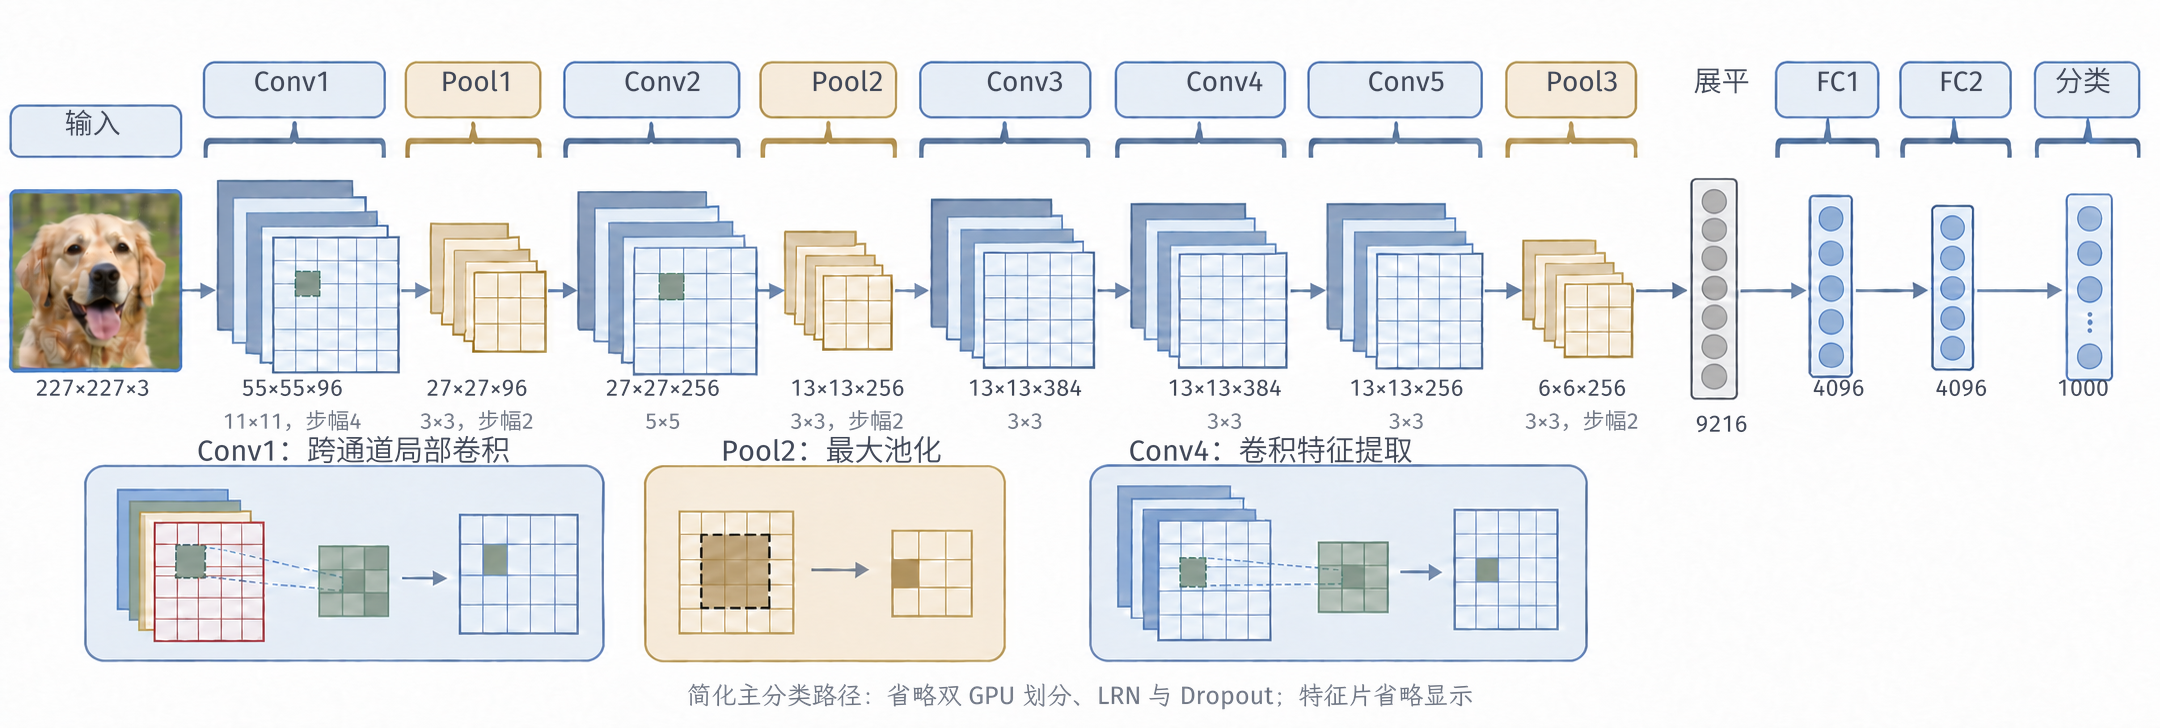
\includegraphics[width=169.000mm]{figures/03-models/02-neural-network-models/generated/cnn-alexnet/figure.png}
  \caption{AlexNet的五个卷积层与三个全连接层。全部主路径在一行展开，卷积层、最大池化层与全连接层分别绘出；最后一次池化的输出展平为9216维。各层下方给出空间尺寸和通道数，Conv表示卷积，Pool表示池化。下方依次展开Conv1的跨通道卷积、Pool2的最大池化和Conv4的卷积特征提取。网格、叠片和卷积核仅作局部映射示意，各层的实际尺寸与步幅以主链标注为准。此图采用227输入及正文给定的填充约定，省略局部响应归一化、Dropout和原始双GPU的分组细节。}
  \label{fig:cnn-alexnet}
\end{figure*}

容量增加也会把成本集中到尾部。仅9216维到4096维的全连接权重就有$37748736$个，下一层又有$16777216$个；它们与卷积核共享权重的组织不同，是全模型参数量的重要来源。原实现将网络分配到两块GPU，部分层限制跨GPU的通道连接，这也影响了分组方式。ReLU、数据增强和Dropout分别作用于非线性、训练输入变化与正则化；GPU让这些运算可以实际执行，训练设计则规定了参数如何由数据学得。这些条件共同支撑了这套大规模监督系统。

\FloatBarrier

\Needspace{14\baselineskip}
\subsubsection{VGG：以连续小核组织深度}
\label{sec:cnn-vgg}

AlexNet混合不同核尺寸，VGG则研究较规则的小核堆叠。主体使用步长一、填充一的$3\times3$卷积，在阶段末用$2\times2$、步长二的最大池化缩小空间。VGG-16的五个阶段分别含$2,2,3,3,3$个卷积层，通道数为$64,128,256,512,512$；加上三个全连接层，共有16个带权重的层，池化与激活不计入这个数字。VGG-19把后三阶段的卷积数增为四，总计19个带权重层\scite{simonyan2015vgg}

\begin{figure*}[tbp]
  \centering
  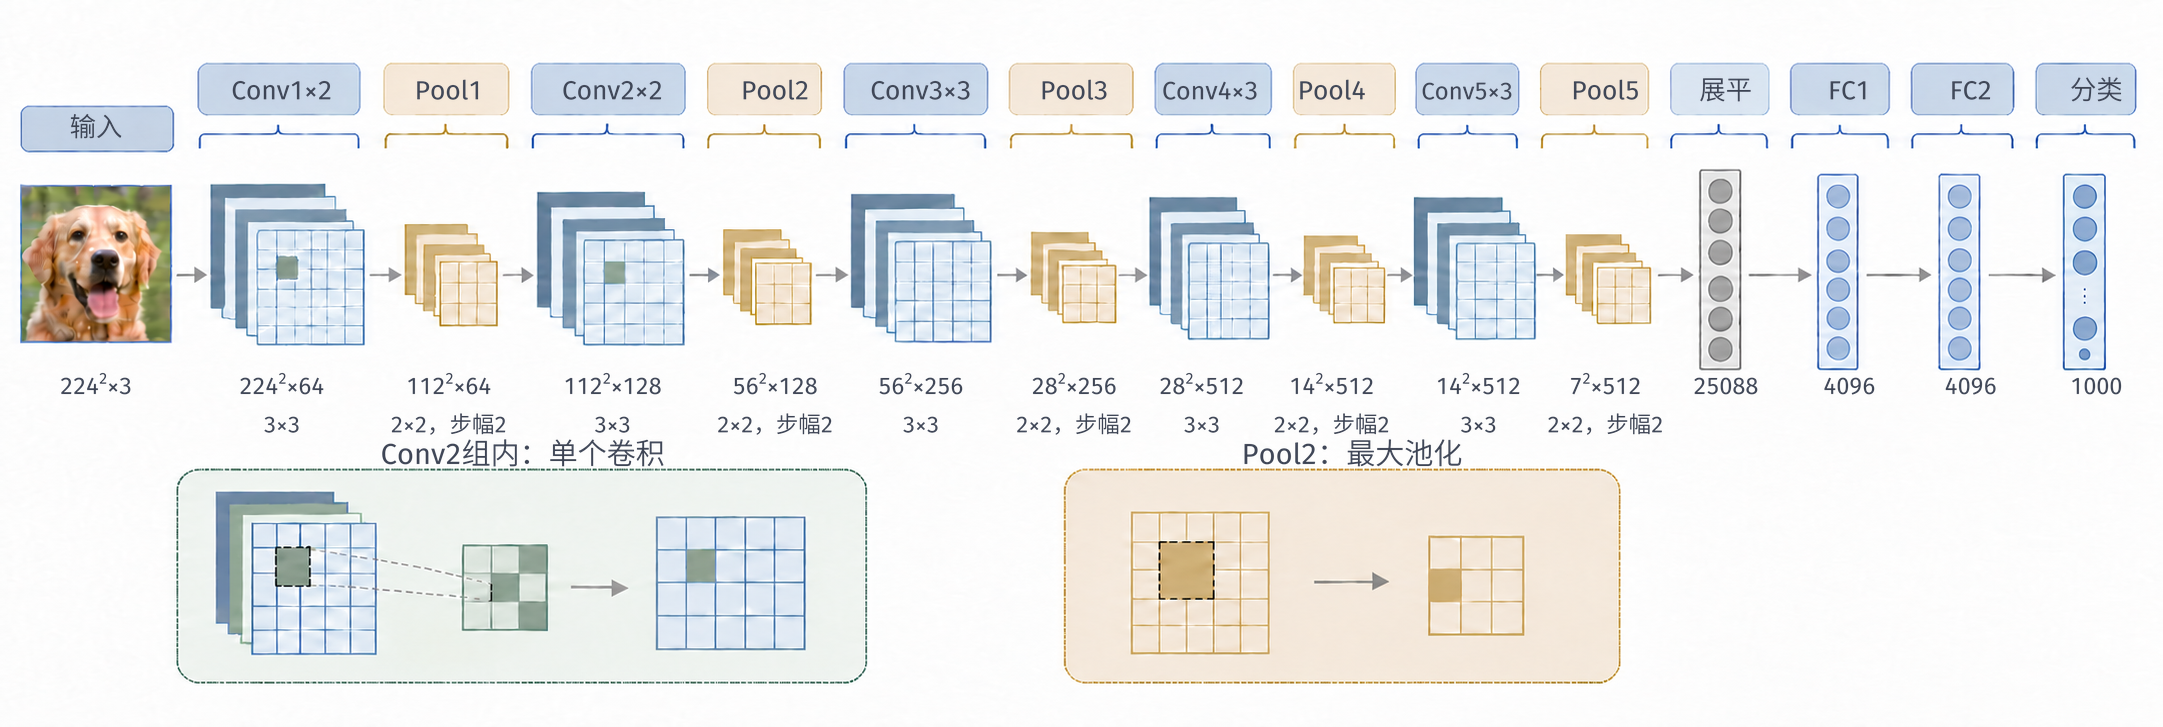
\includegraphics[width=169.000mm]{figures/03-models/02-neural-network-models/generated/cnn-vgg/figure.png}
  \caption{VGG-16的五阶段卷积主体与全连接尾部。沿用AlexNet的特征叠片、池化、灰色展平及全连接图元；层名和尺寸分别置于对应图元上、下。每个Conv组包含标明次数的$3\times3$卷积并保持空间尺寸，其后的池化单独画出、使空间减半。下方展示Conv2组内单个卷积的代表性局部映射及Pool2的最大池化，并不将单个卷积等同于整个卷积组。13个卷积层加三个全连接层构成16个带权重层。网格、叠片数和节点数仅作示意；$a^2\times c$表示$a\times a\times c$。}
  \label{fig:cnn-vgg}
\end{figure*}

连续小核能够逐层扩大感受野。两个步长一的$3\times3$层覆盖$5\times5$跨度，三个覆盖$7\times7$；若各层通道均为$c$且忽略偏置，两个小核用$18c^2$个权重，单个$5\times5$用$25c^2$个。这个权重比较固定了各层通道数。两个小核之间还加入非线性，候选映射由此改变；相同感受野只描述读取范围。

\begin{figure}[htbp]
  \centering
  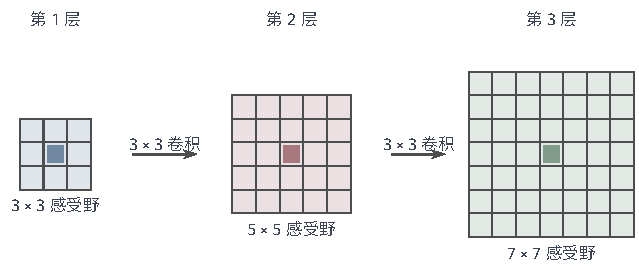
\includegraphics[width=108.158mm]{figures/03-models/02-neural-network-models/tikz/cnn-receptive-field-stack/figure.pdf}
  \caption{三个步长一、无空洞的$3\times3$卷积逐层扩大几何感受野。彩色方格表示一个高层位置在原输入上可能读取的范围，中心实色格只用于对齐位置；跨度依次为$3,5,7$。图没有计入池化、跨位置归一化或边界填充造成的额外依赖。}
  \label{fig:cnn-receptive-field-stack}
\end{figure}

这种规则结构便于分阶段核算形状，但高分辨率阶段的活动值与乘加仍然很大，经典VGG的4096单元全连接尾部也有大量参数。增加深度时仍需合适的训练与正则化。VGG用统一的小核组织深度，串联变换中的梯度传播与训练退化仍需通过学习方法和连接设计处理。

\FloatBarrier

\subsubsection{GoogLeNet：在模块内分配多个尺度}
\label{sec:cnn-googlenet}

连续小核把不同尺度安排在不同深度。若希望同一层同时处理不同范围，可以把输入送入并行分支。\term{Inception模块}将同一输入分别交给$1\times1$、$3\times3$、$5\times5$局部处理及池化分支，再沿通道轴拼接。较大核前先用$1\times1$压缩通道，池化分支保持空间尺寸后也可用逐点卷积调节通道。各分支需要相同高、宽，通道数则可以不同，见图~\ref{fig:cnn-inception}。

\begin{figure*}[tb]
  \centering
  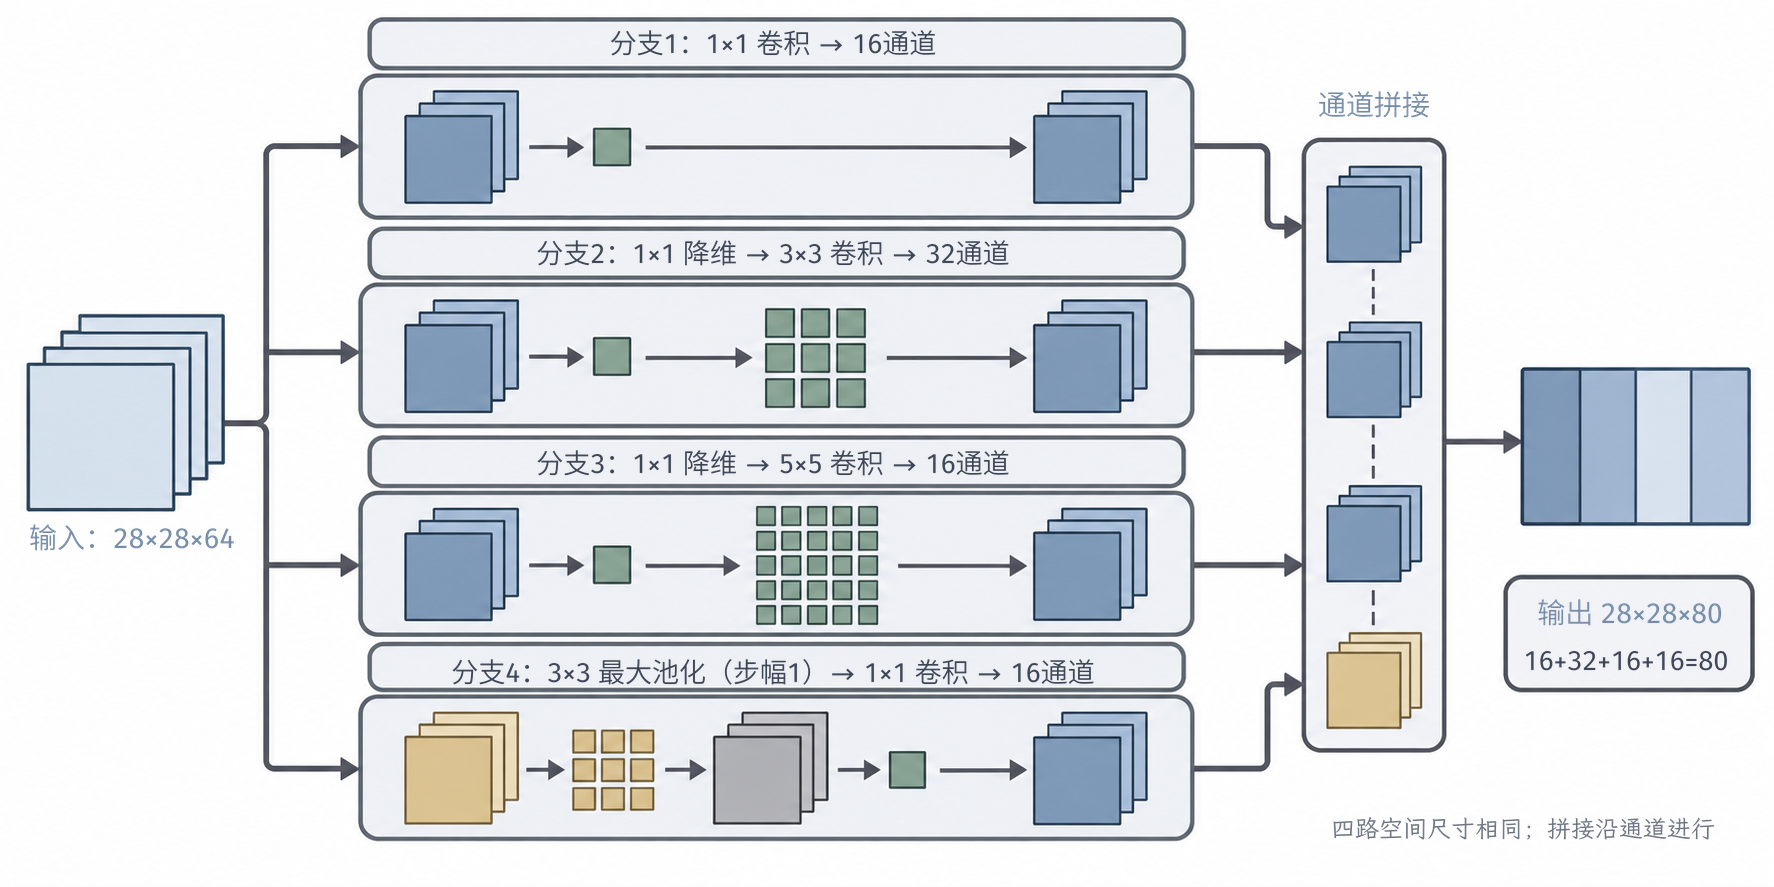
\includegraphics[width=150.199mm]{figures/03-models/02-neural-network-models/generated/cnn-inception/figure.png}
  \caption{一个Inception模块的四分支教学配置。输入为$28\times28\times64$；四条分支分别输出16、32、16、16个通道，保持同一空间尺度，拼接得到$28\times28\times80$。中间的逐点卷积先压缩通道，最大池化采用步长一及same填充。圆角方框表示处理算子，各分支的标签给出核尺寸或通道数；右侧拼接框沿通道合并四路输出。四条路径实际并行，激活省略。}
  \label{fig:cnn-inception}
\end{figure*}

图中$3\times3$分支先将通道从64压到16，再输出32个通道，权重数为$64\times16+9\times16\times32=5632$；直接从64映射到32需要$18432$个。节省来自中间通道压缩，压缩也会限制该分支的表示。拼接保留分支间的区别，没有像相加那样把对应通道混合；后续卷积再学习如何组合这些通道。

经典GoogLeNet先用普通卷积与池化形成$28\times28\times192$特征，再堆叠九个Inception模块，按两、五、两个模块分成三个尺度阶段；两个阶段间池化将空间降为14和7。末端$7\times7\times1024$特征经全局平均池化形成1024维向量，再作1000类分类。训练时，在中间层加入辅助分类器，让较浅位置也收到任务损失；推理时使用主分类路径。图~\ref{fig:cnn-googlenet}展示主路径，原论文按最长路径计22个带参数层，一个Inception模块内部则包含多条路径和多个卷积\scite{szegedy2015googlenet}

\begin{figure*}[tbp]
  \centering
  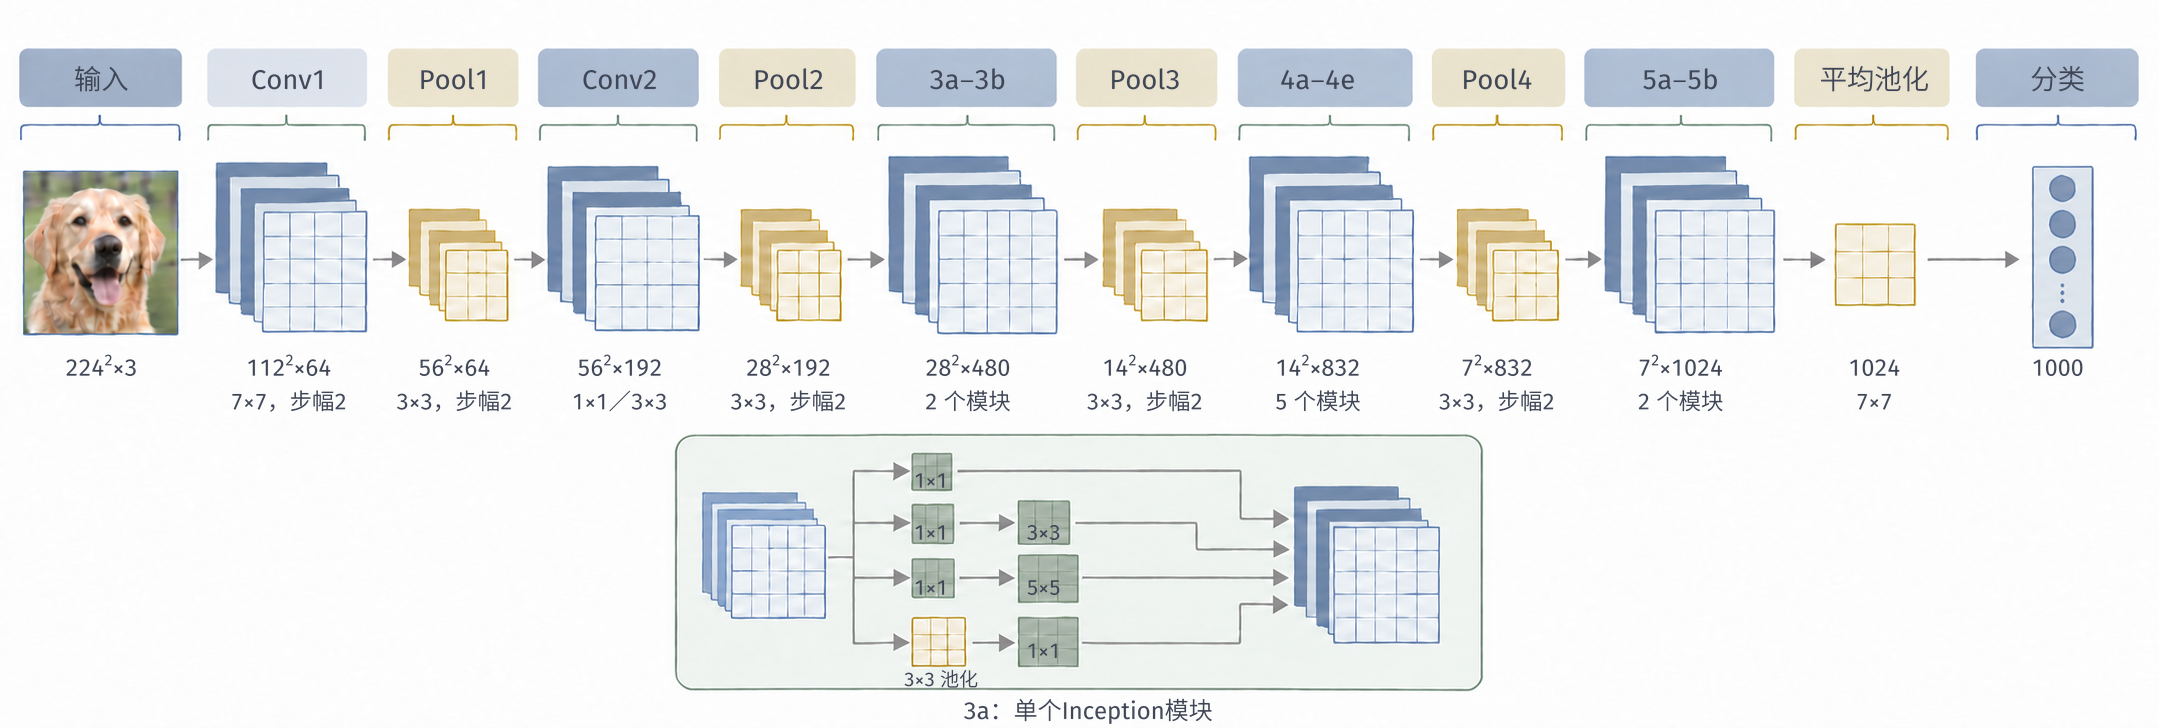
\includegraphics[width=169.000mm]{figures/03-models/02-neural-network-models/generated/cnn-googlenet/figure.png}
  \caption{经典GoogLeNet的主分类路径。卷积前端把$224\times224$输入变成$28\times28\times192$；两个、五个、两个Inception模块组成三个阶段，阶段间池化改变空间尺度。各阶段末的通道数为480、832和1024，全局平均池化后接1000类分类器。辅助分类分支省略，下方以3a为代表展开单个Inception模块的四分支组织，主链的3a--3b组实际包含两个模块；分支机制见图~\ref{fig:cnn-inception}。}
  \label{fig:cnn-googlenet}
\end{figure*}

GoogLeNet用多分支增加同层处理方式，用逐点卷积控制大核分支的成本，并以全局汇聚替代庞大的全连接尾部。代价是分支调度、拼接和更多中间特征，理论乘加预算仍需结合实现分析。表~\ref{tab:cnn-classic-architectures}把四种架构放回共同的问题：它们如何从局部形成整体表示，又将计算与参数放在何处。

\FloatBarrier

\begin{table*}[htb]
  \centering
  \begin{tabularx}{\linewidth}{@{}lXX@{}}
    \toprule
    架构 & 主体组织 & 理解结构时的侧重点\\
    \midrule
    LeNet & 卷积与可学习降采样交替 & 局部到整体；部分连接及原始输出约定\\
    AlexNet & 五个卷积层与较大全连接尾部 & 通道容量、训练机制、GPU分组及尾部成本\\
    VGG & 连续小核，阶段间池化 & 感受野、深度、规则结构及活动值成本\\
    GoogLeNet & 多尺度分支、通道压缩与拼接 & 同层并行处理、计算预算与整体汇聚\\
    \bottomrule
  \end{tabularx}
  \caption{经典卷积网络的组织方式。各行比较计算结构，没有在不同训练设置之间比较准确率。层数、输入形状和读出方式均应结合具体版本理解。}
  \label{tab:cnn-classic-architectures}
\end{table*}

\section{参数学习}
\label{sec:cnn-learning}

卷积网络仍按前章的链式法则学习。结构带来的区别是：一个核权重在许多位置出现，一个输入又可能被多个窗口读取。因此，初始化应按局部连接数定尺度，反向传播则必须汇总所有重复使用的贡献。

\subsection{参数初始化}
\label{sec:cnn-initialization}

对普通卷积，一个输出单元读取$k_hk_wc_{\mathrm{in}}$个值，故通常取
\begin{equation}
  \mathrm{fan\text{-}in}=k_hk_wc_{\mathrm{in}},\qquad
  \mathrm{fan\text{-}out}=k_hk_wc_{\mathrm{out}}\text{。}
  \label{eq:cnn-fans}
\end{equation}
后者按内部位置、步长为一的连接估计，每个输入向多个输出位置及通道贡献；边界、跨步和分组会改变实际连接数。初始化实现一般采用固定的核级约定，应区分这一约定与每个位置的精确计数。

设初始权重独立、零均值、方差为$v$，与输入独立，偏置为零，各输入元素二阶矩为$q$。不同权重的交叉项均值为零，即使相邻像素相关，仍可在这个初始化模型下得到
\[
  \mathbb E[z_{i,j,o}^2]=k_hk_wc_{\mathrm{in}}vq
\]
用于内部位置的尺度估计。若预激活分布关于零对称，ReLU截去负半轴会使二阶矩减半，所以前向He初始化取
\begin{equation}
  w_{a,b,c,o}\sim\mathcal N\!\left(0,
          \frac{2}{k_hk_wc_{\mathrm{in}}}\right)\text{。}
  \label{eq:cnn-he-initialization}
\end{equation}
这与前章一致，分母变为局部输入连接数，而非整张图像的像素数。偏置可以初始化为零；不同核仍需要不同的随机权重，以打破输出通道之间的对称性\scite{he2015rectifiers}

对中心附近近似单位斜率的激活，Glorot初始化可用方差$2/(\mathrm{fan\text{-}in}+\mathrm{fan\text{-}out})$折中前后向尺度。分组层的局部fan-in需除以组数；只有一个空间核的逐通道层，每个输出读取$k_hk_w$个值。跨步卷积中，每个输入参与的输出窗口更少且可能随位置变化，简单独立性估计也不会捕捉共享权重造成的空间相关。初始化提供的是起始尺度依据，训练中还需检查实际活动值与梯度，不能把这些近似当成全过程保证。

\subsection{卷积层反向传播}
\label{sec:cnn-backpropagation}

以式\eqref{eq:cnn-batch-objective}的批平均损失$L_B$为求导对象，记上游传到卷积预激活的梯度为$\delta_{t,i,j,o}=\partial L_B/\partial z_{t,i,j,o}$，其中$t\in B$。这个导数包含整批所有损失项的影响，不只是样本$t$自身的损失。若已知的是紧接卷积的激活输出梯度，需先乘$\sigma'(z_{t,i,j,o})$；若中间还有归一化，则按前向相反顺序对其求导。特别是训练态BN，必须经过完整批统计量的计算图，才能取得这里的$\delta$。以下采用式\eqref{eq:cnn-layer-forward}，并固定零填充约定。

同一权重$w_{a,b,c,o}$在各样本及各输出位置重复使用，因此链式法则给出
\begin{equation}
  \begin{aligned}
    \frac{\partial L_B}{\partial w_{a,b,c,o}}
      &=\sum_{t\in B}\sum_{i=0}^{h'-1}\sum_{j=0}^{w'-1}
         \delta_{t,i,j,o}\widetilde x_{t,u(i,a),v(j,b),c},\\
    \frac{\partial L_B}{\partial b_o}
      &=\sum_{t\in B}\sum_{i=0}^{h'-1}\sum_{j=0}^{w'-1}
         \delta_{t,i,j,o}\text{。}
  \end{aligned}
  \label{eq:cnn-parameter-gradients}
\end{equation}
每次使用该权重都会产生一项局部导数，共享参数的总导数就是这些项之和。不同位置的贡献可以相互加强，也可以抵消；参数共享并不要求所有位置产生相同响应或相同梯度。这里$\delta$已包含批平均的$1/|B|$，汇总时不再除以批量大小。只有前向映射逐样本独立时，才可先由单样本损失分别求导，再在批量上平均。

一个卷积输入$x_{t,u,v,c}$可能参与本样本的多个输出窗口，也可能连接多个输出通道。将卷积局部映射中所有包含它的项找出，得到
\begin{equation}
  \frac{\partial L_B}{\partial x_{t,u,v,c}}
  =\sum_{i,j,o}\sum_{a,b}
    \delta_{t,i,j,o}w_{a,b,c,o}
    \mathbb I\{u=u(i,a),\ v=v(j,b)\}\text{。}
  \label{eq:cnn-input-gradient}
\end{equation}
其中$u,v$在原输入范围内，$\mathbb I$为条件成立时取一的指示函数，求和范围沿用前向计算。索引条件直接选出前向读取了该坐标的项，因此也适用于跨步和空洞。若使用复制或反射填充，一个原输入还可能对应多个扩展位置，需把这些位置的梯度再累加回来；其索引累积关系随填充映射改变。

矩阵形式揭示了它与转置卷积的联系。固定参数时，将每个样本的张量展平，前向预激活为$\bm z_t=\bm C\bm x_t+\bm b_{\mathrm{rep}}$，$\bm b_{\mathrm{rep}}$表示各位置重复的偏置；把$\delta_{t,i,j,o}$展平为$\bm\delta_t$，就有
\begin{equation}
  \nabla_{\bm x_t}L_B=\bm C^\top\bm\delta_t\text{。}
  \label{eq:cnn-backprop-transpose}
\end{equation}
输入梯度正是前向线性算子的转置作用。数据展开实现则先把每个窗口的梯度算出来，再把各列放回输入坐标，并累加重叠部分；这个回填步骤常称为col2im，同一输入坐标对应的窗口梯度在此相加。

仍用式\eqref{eq:cnn-matrix-example}，取仅含这一个输入的批量，不加归一化、不填充、步长一，令$L_B$为全部互相关输出之和。九个输出的$\delta$均为一，则
\begin{equation}
  \nabla_{\bm K}L_B=
    \begin{bmatrix}54&63\\90&99\end{bmatrix},\qquad
  \nabla_{\bm X}L_B=
    \begin{bmatrix}
      1&1&1&0\\1&0&0&-1\\1&0&0&-1\\0&-1&-1&-1
    \end{bmatrix}\text{。}
  \label{eq:cnn-gradient-example}
\end{equation}
例如左上核权重汇总九个窗口的左上元素，和为$54$；$x_{1,1}=6$既以系数$1$参与一个窗口，也以系数$-1$参与另一个窗口，两项相消。虽然某些核权重当前为零，它们的梯度仍可非零，因为改变该权重会立即改变相应输出。偏置梯度为$9$。这个例子把“共享参数累积”与“重叠输入累积”区分开来。

图~\ref{fig:cnn-backprop-shared-overlap}在同一输入与共享核上展开这两种累积。左侧按核坐标收集窗口贡献，右侧按输入坐标收集读取该位置的贡献。

\begin{figure*}[htbp]
  \centering
  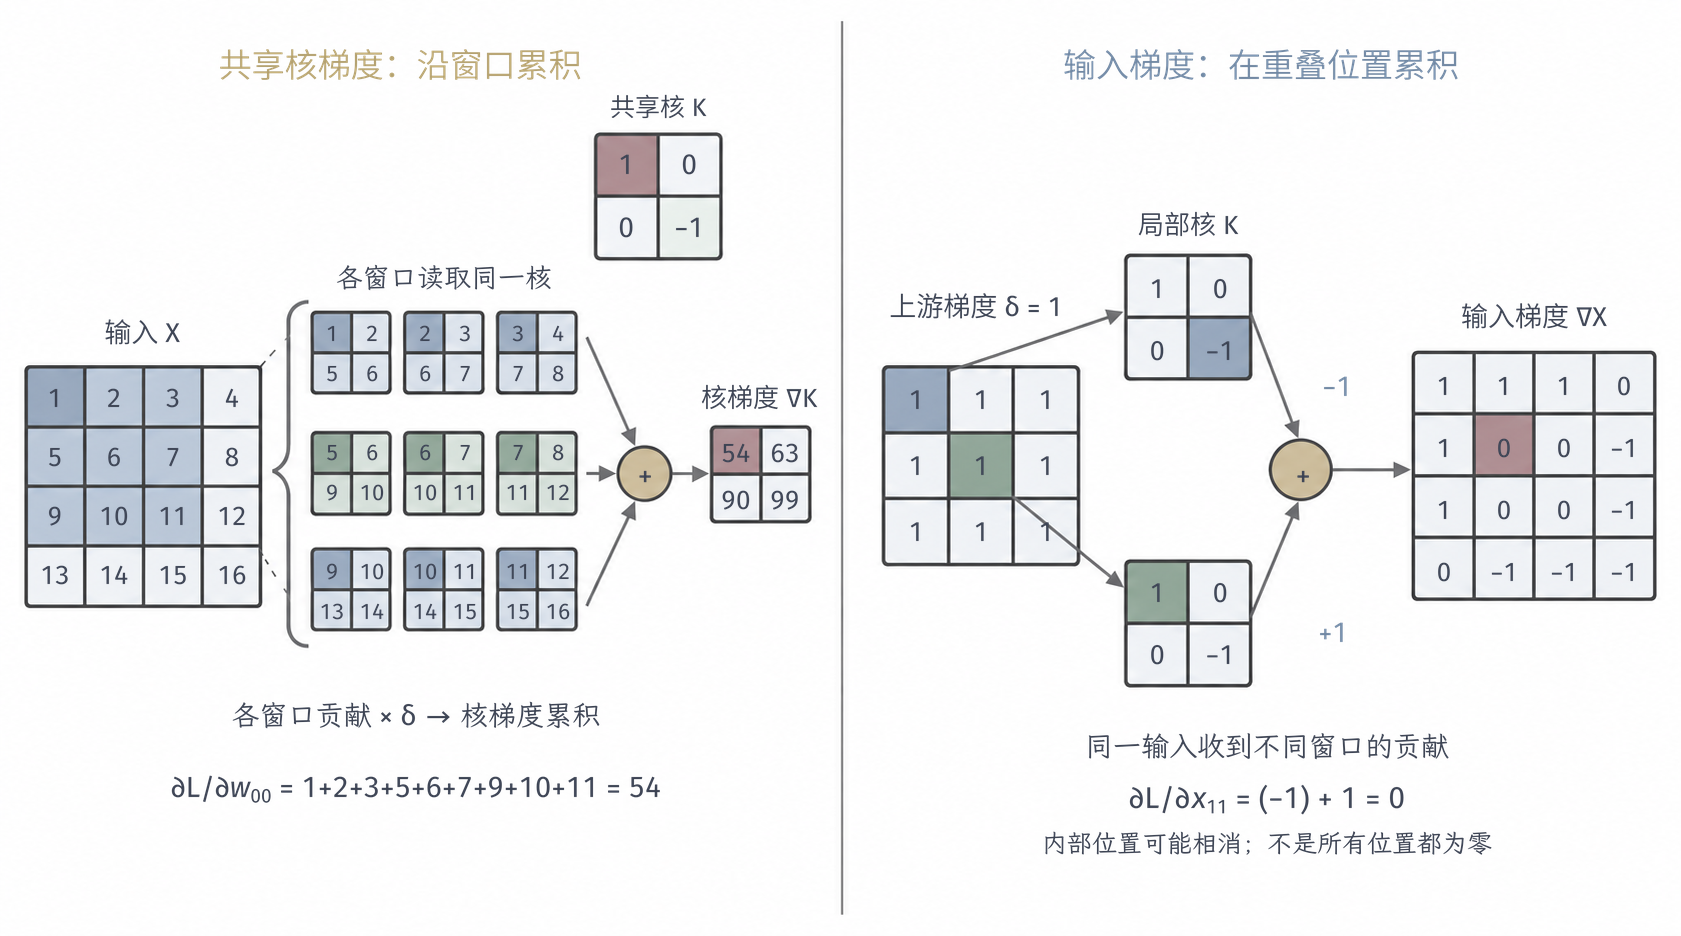
\includegraphics[width=142.325mm]{figures/03-models/02-neural-network-models/generated/cnn-backprop-shared-overlap/figure.png}
  \caption{式~\eqref{eq:cnn-gradient-example}中的两种梯度累积。输入为按行排列$1$至$16$的$4\times4$矩阵，核为$(1,0;0,-1)$，步长一、无填充，损失为九个输出之和。左图汇总九个窗口对同一核参数的贡献；右图突出$x_{1,1}=6$的两项非零贡献，二者相消；另两项贡献因对应核值为零而为零。}
  \label{fig:cnn-backprop-shared-overlap}
\end{figure*}

\subsection{池化层反向传播}
\label{sec:cnn-pooling-backpropagation}

池化没有标准的可学习参数，但它决定上游梯度怎样返回输入。仍对完整批损失求导，设池化输出的梯度为$g_{t,i,j,c}=\partial L_B/\partial y_{t,i,j,c}$。平均池化对每个参与的元素具有相同导数，因此
\begin{equation}
  \frac{\partial L_B}{\partial x_{t,u,v,c}}
  =\sum_{i,j}\frac{g_{t,i,j,c}}{q_{i,j}}
                  \mathbb I\{(u,v)\in\Omega_{i,j}\}\text{。}
  \label{eq:cnn-average-pooling-gradient}
\end{equation}
分母必须与前向平均采用的计数相同。窗口重叠时，一个输入收到多项；全局平均池化则将某通道的上游梯度均分给该通道全部位置。

最大池化在最大值唯一时，只对被选中的元素有非零导数。前向计算记录其位置$(u^*_{t,i,j,c},v^*_{t,i,j,c})$，后向使用同一位置：
\begin{equation}
  \frac{\partial L_B}{\partial x_{t,u,v,c}}
  =\sum_{i,j}g_{t,i,j,c}
       \mathbb I\{(u,v)=(u^*_{t,i,j,c},v^*_{t,i,j,c})\}\text{。}
  \label{eq:cnn-max-pooling-gradient}
\end{equation}
若多个元素并列最大，函数在该点不可微；实现可以按固定规则选择一个位置，也可以采用最大值集合上的合法次梯度分配。后向采用与前向对应的选择或次梯度规则。同一元素若是多个重叠窗口的最大值，会收到这些窗口梯度的和。

对式\eqref{eq:cnn-pooling-example}，令四个输出梯度均为一。平均池化使每个输入收到$1/4$，最大池化只让原矩阵中的$6,8,14,16$各收到$1$。回传规则因此保留了两种汇聚方式的区别：平均把影响均分，最大把影响路由到当前胜出的位置。卷积与池化梯度接入前章的反向传播后，就能联合更新整个网络；优化器和学习率的通用选择由后续训练章讨论。

\section{支持更深的网络结构}
\label{sec:cnn-deep-structures}

连续堆叠卷积可以扩大感受野并增加非线性组合，却也使信息和梯度经过更长的变换链。前章已说明，Jacobian矩阵连乘可能放大或衰减梯度。即使初始化和归一化让训练开始收敛，更深的普通串联网络仍可能出现更高的训练误差。增加层数后训练误差反而上升，称为\term{退化问题}（degradation problem）。该现象发生在训练集上，涉及更深参数化的求解困难。ResNet论文在其图像实验中报告并研究了这一现象\scite{he2016resnet}

跨层连接允许部分信息绕过某些变换。下面比较三种组织方式：直接相加、用门选择相加，以及保留旧特征再拼接新特征。它们都可以保持前馈计算，但改变了中间表示和梯度路径。

\subsection{残差连接与ResNet}
\label{sec:cnn-resnet}

若新增的一组层暂时无须改变输入，普通串联模块仍要学出恒等映射。\term{残差连接}（residual connection）把输入直接加到变换分支的结果上，使该分支只学习相对于输入需要改动的部分。将输入特征展平为$\bm x\in\mathbb R^d$，维度相同时，模块写为
\begin{equation}
  \bm y=\bm x+\bm F_{\bm\theta}(\bm x)\text{。}
  \label{eq:cnn-residual-block}
\end{equation}
其中$\bm F_{\bm\theta}:\mathbb R^d\to\mathbb R^d$由若干卷积、归一化和激活组成。若目标映射接近恒等，残差分支只需接近零。这里的“残差”是模块输出相对于输入的差，不是标签减去预测值的训练误差。

图~\ref{fig:cnn-resnet}展开一个基本模块中的层与残差连接。上方旁路把输入直接送到加法节点，主分支则计算需要叠加的变换；图中的模块还在相加后施加一次ReLU。
\begin{figure*}[htbp]
  \centering
  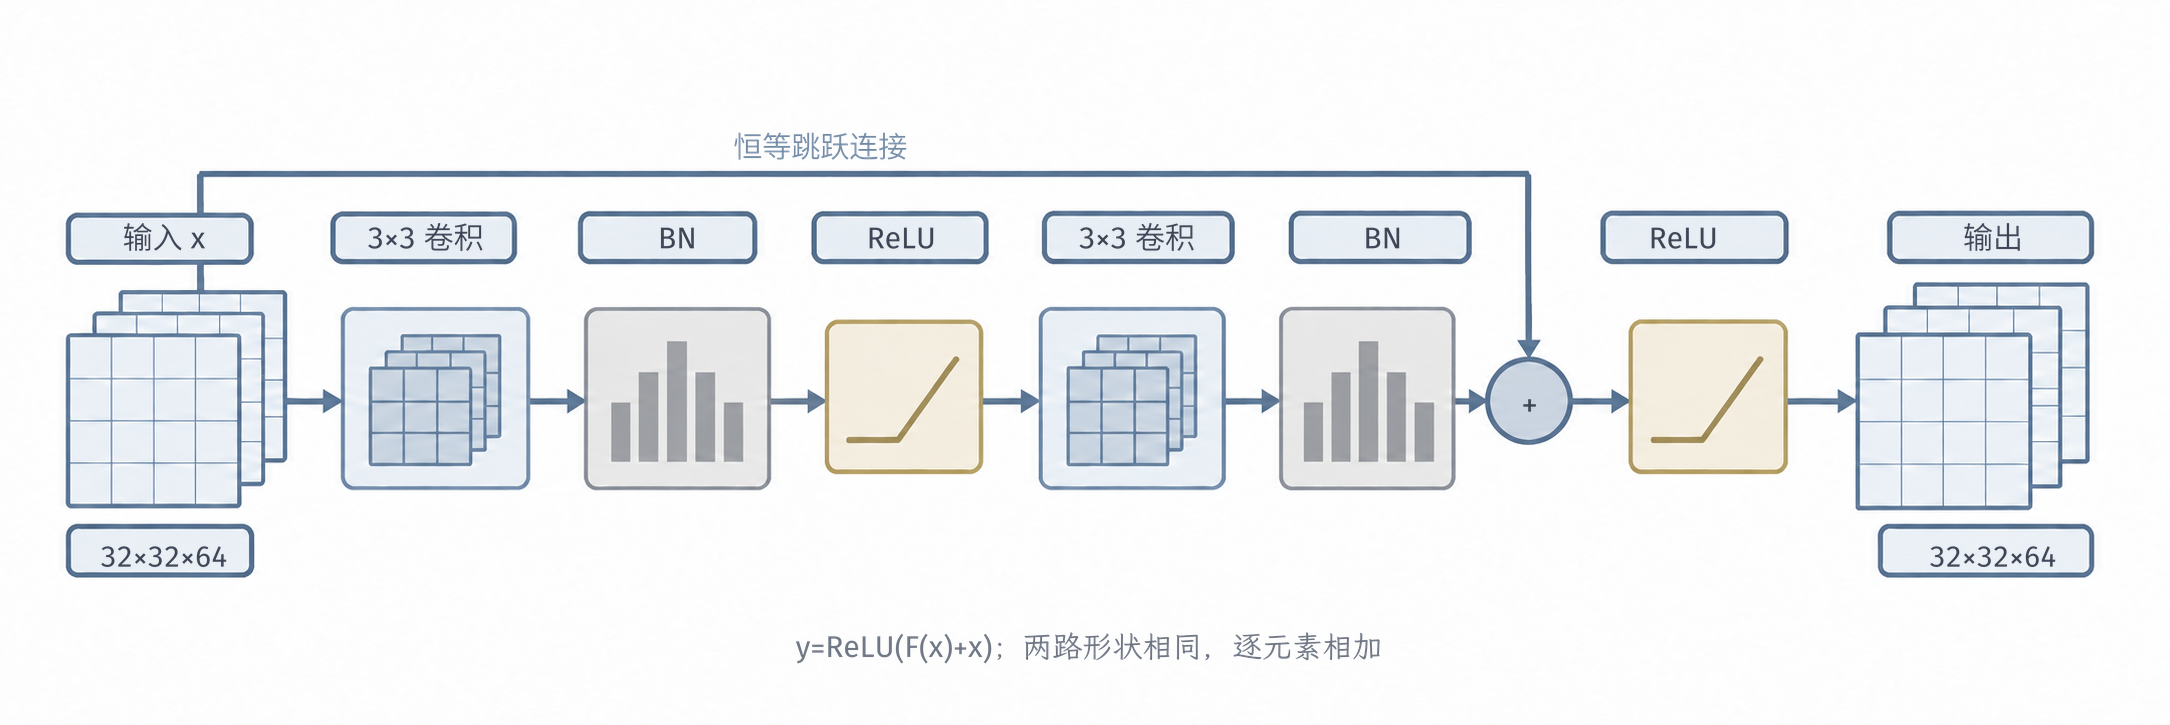
\includegraphics[width=169.000mm]{figures/03-models/02-neural-network-models/generated/cnn-resnet/figure.png}
  \caption{残差基本模块中的逐层变换与恒等旁路。主分支依次经过$3\times3$卷积、BN、ReLU及第二个$3\times3$卷积、BN，再与直接传来的输入逐元素相加并激活。两次卷积均保持$32\times32\times64$形状，上方旁路跳过主分支的变换。圆角方框表示算子，圆形加号节点表示逐元素相加；改变尺度或通道时，旁路需要投影。}
  \label{fig:cnn-resnet}
\end{figure*}
\FloatBarrier

下面只考察相加本身，暂不在相加后施加额外激活；含训练态BN时，$\bm x$应包含参与统计的整批特征。在可微位置，令$\bm J_F=\partial\bm F/\partial\bm x$。输入的微小变化$\mathrm d\bm x$沿两条路径分别产生$\mathrm d\bm x$与$\bm J_F\,\mathrm d\bm x$，相加后有
\[
  \mathrm d\bm y=\mathrm d\bm x+\bm J_F\,\mathrm d\bm x
    =(\bm I+\bm J_F)\,\mathrm d\bm x\text{。}
\]
对标量损失$\ell$，链式法则给出$\mathrm d\ell=(\nabla_{\bm y}\ell)^\top\mathrm d\bm y$。代入上式，再与$\mathrm d\ell=(\nabla_{\bm x}\ell)^\top\mathrm d\bm x$比较，就得到
\begin{equation}
  \begin{aligned}
    \frac{\partial\bm y}{\partial\bm x}&=\bm I+\bm J_F,\\
    \nabla_{\bm x}\ell&=(\bm I+\bm J_F)^\top\nabla_{\bm y}\ell\\
      &=\nabla_{\bm y}\ell+\bm J_F^\top\nabla_{\bm y}\ell\text{。}
  \end{aligned}
  \label{eq:cnn-residual-gradient}
\end{equation}
末行的第一项直接经过恒等路径，第二项经过残差分支。两项共同决定输入梯度，例如标量分支$F(x)=-x$就有$1+F'(x)=0$，两路贡献恰好相消。多块连乘后，尺度还随各块Jacobian矩阵变化；恒等路径改变了传播结构，整体梯度仍由全部路径决定。

若记相加结果为$\bm z=\bm x+\bm F(\bm x)$，再令$\bm y=\operatorname{ReLU}(\bm z)$，则反向还要先经过ReLU：
\[
  \nabla_{\bm x}\ell
    =(\bm I+\bm J_F)^\top\bm D_{\mathrm{ReLU}}\nabla_{\bm y}\ell\text{。}
\]
在$z_i\neq0$处，$\bm D_{\mathrm{ReLU}}$的第$i$个对角元素为$\mathbb I\{z_i>0\}$；零点按实现选定导数。这层激活也筛选恒等路径传来的贡献，相加结果与最终输出因而具有不同的导数。

当阶段间下采样或改变通道时，输入与分支结果不能直接逐元素相加。可用投影$\bm P$调整形状，写为$\bm y=\bm P\bm x+\bm F(\bm x)$；例如用跨步$1\times1$卷积同时改变空间尺寸与通道。此时跨层路径的Jacobian矩阵是$\bm P$，不再是$\bm I$，合并输出的Jacobian矩阵相应变为$\bm P+\bm J_F$。选择恒等或投影，取决于两条分支的形状和希望保留的映射。

ResNet在多个阶段堆叠残差模块。基本模块常用两个$3\times3$卷积；瓶颈模块用$1\times1$压缩通道、$3\times3$处理空间、再用$1\times1$恢复通道，以控制主体计算。经典版本在相加后使用激活。不同版本通过激活位置、旁路投影和下采样所在分支确定计算图；这些选择共同影响信息和梯度路径。

ResNet-18的主干分为四个阶段：对$224\times224$输入，前端$7\times7$卷积取步长二、填充三，产生$112\times112$特征；接BN、ReLU及$3\times3$、步长二、填充一的最大池化，得到$56\times56$网格。四个阶段分别使用64、128、256、512个通道，每个阶段包含两个基本模块；后三阶段的首模块将空间减半，并用投影匹配相加形状。末端全局平均池化与分类层完成整体读出。

\subsection{门控连接与Highway网络}
\label{sec:cnn-highway}

直接相加始终保留输入并叠加变换；若希望根据当前输入控制两条路径的比例，可以让网络学习一个门。\term{Highway网络}（Highway network）用控制门调节哪些坐标更多采用新变换、哪些更多保留原值。维度相同、保留门与变换门互补时，
\begin{equation}
  \begin{aligned}
    \bm g(\bm x)&=\operatorname{Sigmoid}(\bm G(\bm x)),\\
    \bm y&=\bm g(\bm x)\odot\bm F(\bm x)
            +(\bm1-\bm g(\bm x))\odot\bm x\text{。}
  \end{aligned}
  \label{eq:cnn-highway-block}
\end{equation}
其中$\bm F$为变换路径，$\bm G$产生与输入同形状的门得分，Sigmoid逐元素把门值限制在$(0,1)$。在卷积模块中，$\bm F$和$\bm G$都可使用共享局部计算。门值接近零时以保留路径为主，接近一时以变换路径为主。原工作采用负的门偏置，使初始门倾向保留输入，帮助很深的网络开始学习\scite{srivastava2015highway}

门值随输入变化，这一变化也参与输出导数。记$\operatorname{Diag}(\bm v)$为以向量$\bm v$作对角线的矩阵，$\bm J_g$为门的Jacobian矩阵，则
\begin{equation}
  \begin{aligned}
    \bm J_y={}&\operatorname{Diag}(\bm g)\bm J_F
      +\operatorname{Diag}(\bm1-\bm g)\\
      &+\operatorname{Diag}(\bm F(\bm x)-\bm x)\bm J_g\text{。}
  \end{aligned}
  \label{eq:cnn-highway-gradient}
\end{equation}
末项来自门值随输入变化的影响。负偏置使门初始更接近保留路径，也可能让Sigmoid进入导数较小的区域，门参数的学习仍需合适尺度。Highway增加了可学习的路由及其参数成本；式\eqref{eq:cnn-highway-block}中两条系数之和为一，与ResNet无门控的直接相加具有不同约束。

图~\ref{fig:cnn-highway}展开变换、门和保留路径，两个逐元素乘法节点分别调节变换结果与原输入，再由相加节点合并。三条路径都保持$h\times w\times c$形状，门按位置和通道决定缩放系数；改变形状的模块还要为保留路径安排投影，并使门与两路结果具有匹配的目标形状。

\begin{figure*}[tbp]
  \centering
  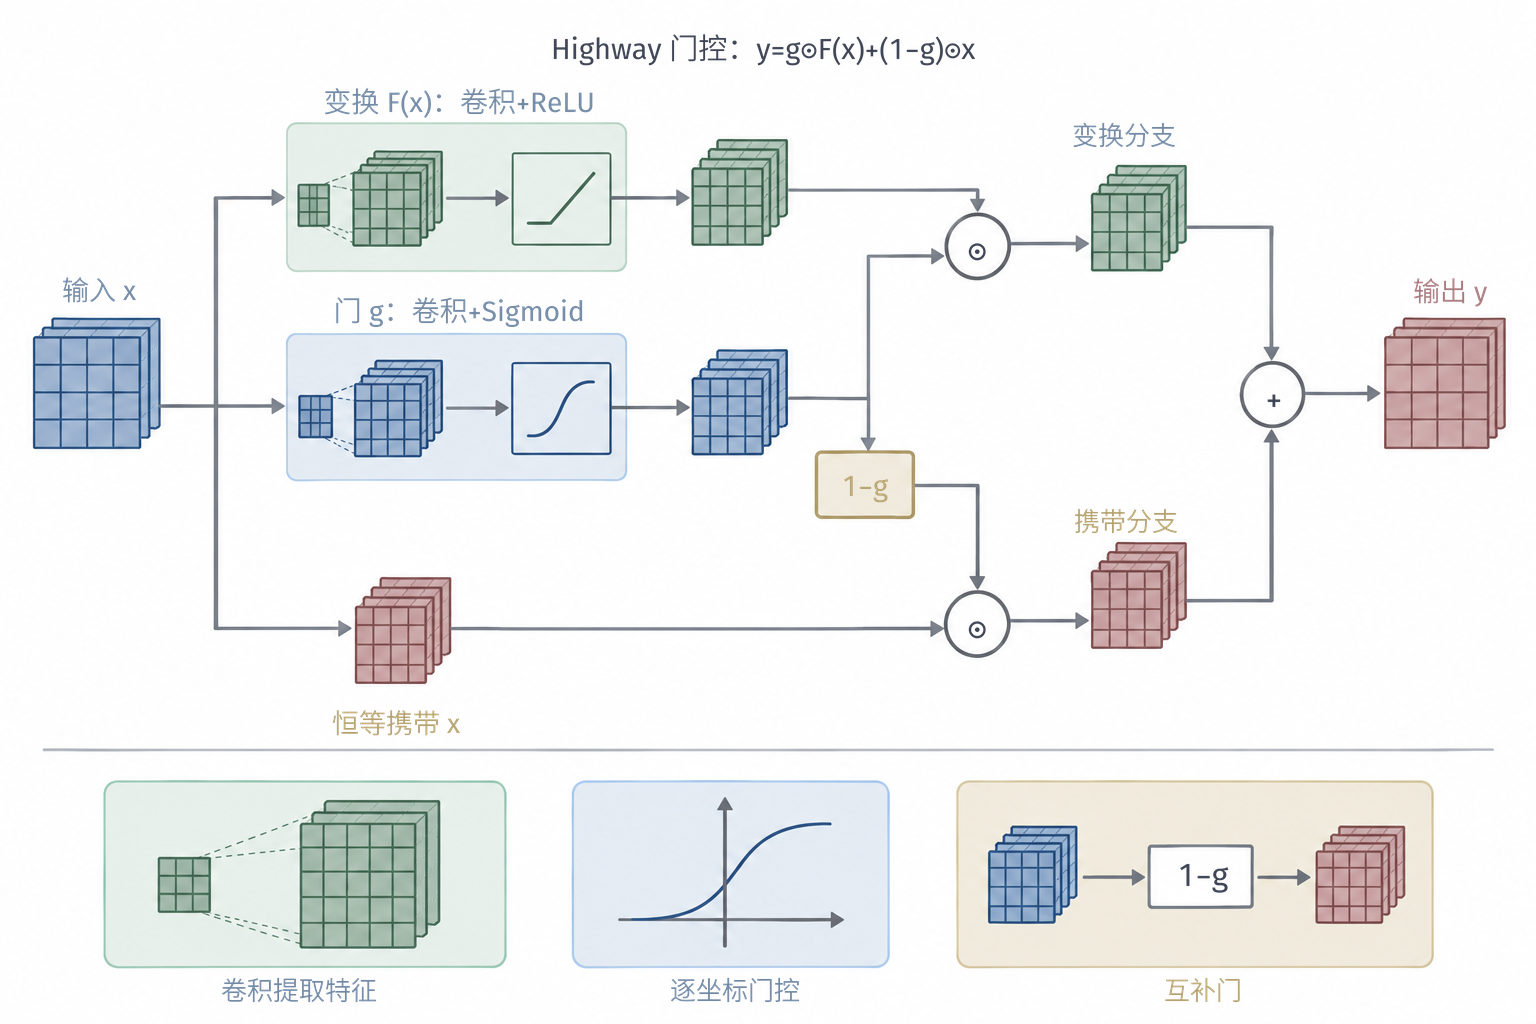
\includegraphics[width=130.048mm]{figures/03-models/02-neural-network-models/generated/cnn-highway/figure.png}
  \caption{同形状卷积Highway模块。上方卷积与ReLU产生$\bm F(\bm x)$，门路径经卷积与Sigmoid产生$\bm g$，保留路径传递原输入；两个$\odot$节点分别计算$\bm g\odot\bm F(\bm x)$和$(\bm1-\bm g)\odot\bm x$，再由$+$节点相加。所有特征与门具有同一空间、通道形状，圆角方框表示各条路径的处理算子。}
  \label{fig:cnn-highway}
\end{figure*}

\FloatBarrier

\subsection{密集连接与DenseNet}
\label{sec:cnn-densenet}

残差相加把旧特征和新特征合在相同通道中。若希望后层仍能分别读取先前各层的特征，可以沿通道轴保留它们。\term{密集连接}（dense connection）使一个块内的每层读取全部先前层的输出；DenseNet按这种方式构造卷积模块：
\begin{equation}
  \bm H^{(\ell)}=\bm F_\ell\!\left(
      [\bm H^{(0)},\bm H^{(1)},\ldots,\bm H^{(\ell-1)}]
    \right)\text{。}
  \label{eq:cnn-dense-block}
\end{equation}
方括号表示通道拼接，不是逐元素相加；块内空间高、宽必须一致。$\bm H^{(0)}$为块的输入，各层只产生新的通道，旧特征仍可供更后层直接读取\scite{huang2017densenet}

若块输入有$c_0$个通道，每层新增$k$个通道，$k$称为\term{增长率}（growth rate），即每层增加的特征数。第$\ell$层输入有$c_0+(\ell-1)k$个通道，包含$L$层的整个块输出有$c_0+Lk$个通道。以$c_0=32,k=16,L=4$为例，各层依次读取$32,48,64,80$个通道，最终拼接得到$96$个通道。块间的\term{过渡层}（transition layer）用逐点卷积压缩通道，再通过池化降低空间尺寸，限制持续增长的特征规模。

密集连接提供直接的特征读取和梯度路径，但需要保留更多活动值。若每层只用一个产生$k$个新通道的$3\times3$卷积，忽略偏置，块内权重数为
\begin{equation}
  9k\sum_{\ell=1}^{L}\bigl(c_0+(\ell-1)k\bigr)
  =9k\left(Lc_0+\frac{kL(L-1)}2\right)\text{。}
  \label{eq:cnn-dense-cost}
\end{equation}
固定增长率下，这个简化块的通道相关成本随层数呈二次增长；瓶颈和压缩设计会改变具体成本。残差模块维持相加后的通道数，密集模块保留旧通道并增加新通道，二者以不同方式复用特征，活动值内存与计算量也由各自的通道增长和模块操作决定。


图~\ref{fig:cnn-densenet}从左向右展示一个三层教学密集块：32个初始通道加上三组16个新通道，输出为80个通道。每次变换前的全部特征经旁路保留，再与本层新产生的通道拼接，因而后层仍能读取每个先前层的输出。若在块后接过渡层，可用$1\times1$卷积把80个通道压缩为40个，再通过池化把$32\times32$空间网格缩为$16\times16$。

\begin{figure*}[tbp]
  \centering
  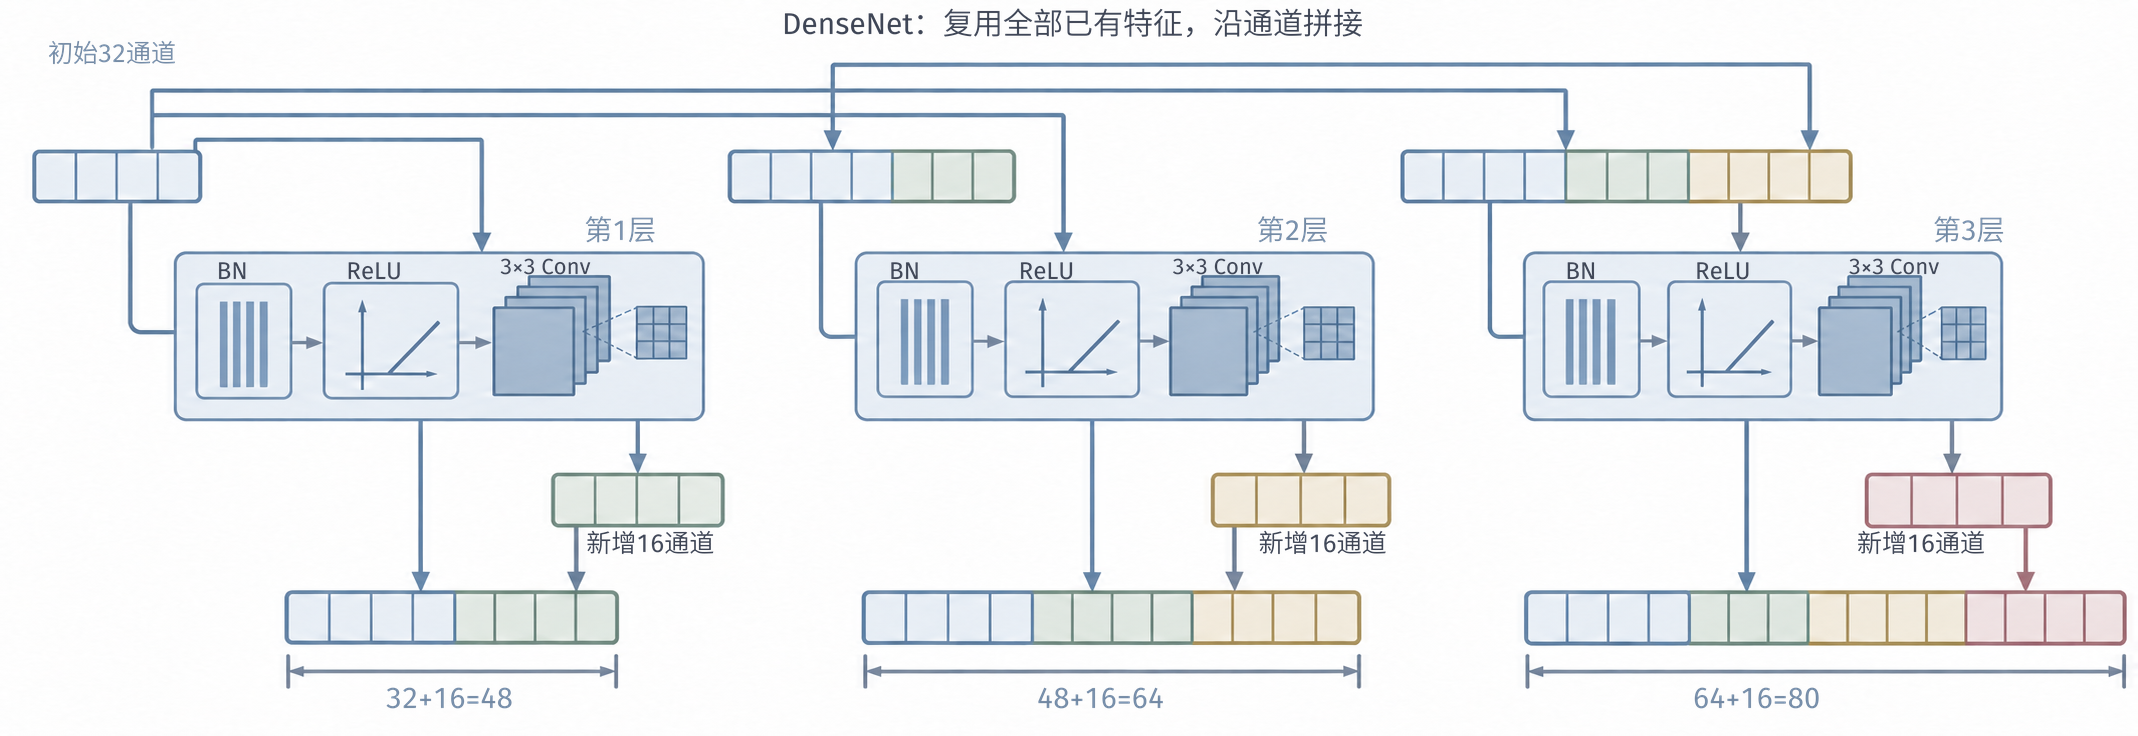
\includegraphics[width=169.000mm]{figures/03-models/02-neural-network-models/generated/cnn-densenet/figure.png}
  \caption{DenseNet的三层教学密集块。各$\bm F_\ell$依次执行BN、ReLU和$3\times3$卷积，保持$32\times32$空间网格并新增16个通道。三次变换分别读取32、48、64个通道；上方旁路保留变换前的全部特征，标出的32、48、64为累计通道数；卷积下方的16为新增通道数。拼接位置将新旧特征沿通道合并，最终得到80个通道。逐次累积拼接等价于保留并向后传递全部先前层的输出，不作逐元素相加。}
  \label{fig:cnn-densenet}
\end{figure*}

\FloatBarrier

\section{理论分析}
\label{sec:cnn-theory}

卷积、池化和跨层连接共同规定候选函数。以下先检查这些结构能否保留目标所需信息，再讨论共享参数的优化，最后考察训练所得预测在新图像上的风险。泛化分析采用$n$个独立同分布训练样本及同分布测试样本，架构和参数约束在抽样前确定；数据相关约束需要另加选择代价。结构是否容纳目标、更新是否得到合适参数，以及这些参数在新样本上的风险，对应不同的分析对象。

\subsection{表达能力}
\label{sec:cnn-expressivity}

卷积把候选映射限制为局部、共享的变换，深度再组合局部模式。若目标要求重复识别同一种平移图案，这种限制与目标吻合；若不同位置必须采用不同规则，就需位置特征或相应读出。固定感受野之外的信息不能在该层直接参与判断，增加深度、核宽或全局读取才会改变这一边界。

池化与下采样可能把多个输入映成同一个表示。如果两个类别所需区分的输入已被映成相同表示，后续层就只能给它们相同输出。函数族的表达能力因此同时取决于参数与结构保留的信息；位置、细节和交互被删除后，扩大后续层仍受这一限制。

\subsection{收敛性}
\label{sec:cnn-convergence}

共享核收到所有位置的梯度之和，反向传播必须包含这些重复使用的贡献；共享减少独立参数，各层非线性与参数乘积仍使端到端目标通常具有非凸结构。对梯度Lipschitz连续且有下界的确定性目标，梯度下降采用固定正步长，且步长不超过一个正的梯度Lipschitz上界的倒数时，可使前$T$轮的平均平方梯度范数具有$O(1/T)$上界；这个驻点指标不保证找到全局最优候选。这个结论针对所给的光滑确定性目标。ReLU、随机批量、归一化和自适应更新分别改变了光滑性、梯度来源或更新规则，其收敛分析需要相应条件；残差路径本身仅规定计算结构。

输入尺度、重叠窗口与整层算子范数改变曲率和梯度尺度，可能影响允许步长；实际速度还包含每轮的计算代价。固定特征上的凸读出与端到端特征学习应分别判断。具体更新方法和训练诊断见第\ref{chap:neural-network-training}章。

\subsection{泛化性}
\label{sec:cnn-generalization}

\subsubsection{输入与数据}
\label{sec:cnn-data-generalization}

样本量首先要按独立信息的来源计数。同一图像中的像素、重叠裁块或同一段视频中的相邻帧通常相关；以独立图像为样本的分析，样本数由图像来源计数。一个图像内重复使用参数可以提供多项梯度贡献，这些贡献仍受同一图像内容的共同影响。按原始图像、对象或采集来源划分训练与测试数据，才与相应的独立证据来源一致。

输入尺寸与尺度需要一起分析。若每个输入元素的绝对值不超过$a$，展平图像的欧氏范数只能粗略保证$\lVert\bm x\rVert_2\leq a\sqrt{hwc_{\mathrm{in}}}$。增大分辨率可能增加有用细节，也可能在范数界中增加复杂度项。按整张图像归一化可以控制总范数，却改变了局部数值尺度；逐通道标准化并不必然控制整图范数。较高分辨率下，固定像素大小的卷积核还覆盖较小的相对区域，因此输入尺寸也改变了结构与任务的配合。

参数共享有价值的条件，是不同位置确实可以由相近规则处理。若同一物体的平移应保持分类标签，共享局部特征与整体汇聚与任务相符；若目标是判断标记是否位于图像左侧，完全舍去位置的读出就可能丢失目标所需信息。对分割，目标轮廓随输入平移，等变表示更贴近输出关系。固定位置、边界和尺度差异都可能使同一个局部图案在不同位置具有不同含义。

可以用一个受限模型把样本量与尺度的作用算清楚。此处只研究单通道标量得分，省去激活和偏置，并在局部线性响应之后作全局平均。设展平输入为$\bm x\in\mathbb R^d$，第$r$个窗口的取数矩阵为$\bm P_r\in\mathbb R^{q\times d}$，共有$m$个窗口。采用零填充且每个窗口内不重复读取同一坐标，定义平均窗口向量
\begin{equation}
  \bm\phi(\bm X)=\frac1m\sum_{r=1}^{m}\bm P_r\bm x,
  \qquad f_{\bm w}(\bm X)=\bm w^\top\bm\phi(\bm X)\text{。}
  \label{eq:cnn-pooled-linear-model}
\end{equation}
其中$\bm w\in\mathbb R^q$为共享核权重。假设抽样前固定$\lVert\bm w\rVert_2\leq\alpha$，输入满足$\lVert\bm x\rVert_2\leq r_x$。取数不会增大单个窗口的范数，再由三角不等式有$\lVert\bm\phi(\bm X)\rVert_2\leq r_x$。对独立随机符号$\varepsilon_t\in\{-1,+1\}$，经验Rademacher复杂度满足
\begin{equation}
  \begin{aligned}
    \widehat{\mathfrak R}_S(\mathcal H)
    &=\frac\alpha n\mathbb E_{\bm\varepsilon}
           \left\lVert\sum_{t=1}^{n}\varepsilon_t\bm\phi(\bm X_t)\right\rVert_2\\
    &\leq\frac\alpha n
         \sqrt{\sum_{t=1}^{n}\lVert\bm\phi(\bm X_t)\rVert_2^2}
     \leq\frac{\alpha r_x}{\sqrt n}\text{。}
  \end{aligned}
  \label{eq:cnn-pooled-rademacher}
\end{equation}
这里$\mathcal H$是满足该核约束的函数空间。等号来自欧氏球上线性函数的最大值，第一条不等式来自均方根上界，交叉项因随机符号独立而消失。窗口数$m$没有显式出现，因为我们控制了平均后的特征范数；这不表示窗口产生了$m$倍独立样本。

若损失取值于$[0,1]$、对得分具有Lipschitz常数$\lambda_{\mathrm{loss}}$，并满足相应可测性条件，由收缩引理和经验复杂度风险界，以至少$1-\delta$的概率，对全部上述模型有
\begin{equation}
  R(f)\leq\widehat R_S(f)
    +\frac{2\lambda_{\mathrm{loss}}\alpha r_x}{\sqrt n}
    +3\sqrt{\frac{\log(2/\delta)}{2n}}\text{。}
  \label{eq:cnn-pooled-risk-bound}
\end{equation}
其中$\delta\in(0,1)$为失效概率，$R$与$\widehat R_S$使用同一损失（风险界参考\BookTheoremRef{thm:rademacher-risk-bound}{第二卷“基础、理论和可信性”的“二分类学习的可学习性”章“Rademacher复杂度给出的期望风险上界”定理}）。这个界针对受约束的线性共享核与有界Lipschitz损失，明确给出了样本数、输入尺度和核约束的作用。深层CNN或无界交叉熵改变了分析对象，需要另外建立复杂度与风险条件。若平均汇聚已经删掉标签需要的位置差异，复杂度很小的模型也可能具有较大的逼近误差。学习判断仍需结合式\eqref{eq:ffn-risk-decomposition}中的逼近、估计和优化三项。

\subsubsection{参数}
\label{sec:cnn-parameter-generalization}

卷积的参数规模由核尺寸与通道数决定，空间共享限制了独立可调的自由度。对固定有限的分段线性架构，可以把参数数和计算结构代入相应容量分析，但还需保留深度、计算单元及共享方式的条件；全连接架构的计数结果也需先核对是否允许这些共享与计算结构。理论部分的VC分析提供最坏情形工具，实际得到的界也可能很松。

参数范数提供另一种约束。一个核展平后得到的$\bm W_{\mathrm{loc}}$描述单个窗口的映射，整个卷积层的$\bm C$却还包括窗口重复与重叠。两者的谱范数一般不同。以步长一、循环边界的一维核$(1,1)$为例，局部行向量范数为$\sqrt2$；输入为常数向量时，整层把该向量放大两倍，整层算子范数实际为$2$。局部核的展平范数描述一个窗口；整层谱范数还包含重叠窗口共同放大的作用。

这个区别可以通过数据展开估计。设一个原输入坐标最多被$\mu$个窗口读取，把所有窗口堆成向量的取数映射记为$\bm E$。零填充下，每个坐标至多被重复$\mu$次，所以$\lVert\bm E\rVert_2\leq\sqrt\mu$。各窗口再独立应用同一局部矩阵，便有
\begin{equation}
  \lVert\bm C\rVert_2
    \leq\sqrt\mu\,\lVert\bm W_{\mathrm{loc}}\rVert_2
    \leq\sqrt\mu\,\lVert\bm W_{\mathrm{loc}}\rVert_{\mathrm F}\text{。}
  \label{eq:cnn-operator-bound}
\end{equation}
其中$\lVert\cdot\rVert_{\mathrm F}$为Frobenius范数。普通步长一的二维窗口有$\mu\leq k_hk_w$；跨步和边界会改变重复次数，复制填充还需重新统计坐标复用。这个上界由最大重复次数估计，各窗口贡献相消时，实际范数可以更小。

在步长一、循环边界的条件下，傅里叶基可以将卷积化为各频率上的通道映射。对每个离散频率$(\omega_1,\omega_2)$，记核对应的复矩阵为$\widehat{\bm W}(\omega_1,\omega_2)\in\mathbb C^{c_{\mathrm{out}}\times c_{\mathrm{in}}}$，则
\begin{equation}
  \lVert\bm C\rVert_2
    =\max_{\omega_1,\omega_2}
       \sigma_{\max}\!\left(\widehat{\bm W}(\omega_1,\omega_2)\right)\text{。}
  \label{eq:cnn-fourier-norm}
\end{equation}
这里$\sigma_{\max}$是最大奇异值，频域核使用与该卷积映射一致的变换约定。Sedghi等系统研究了这种卷积奇异值表示；有限图像的零填充、裁剪或跨步改变了线性算子，这时谱范数应对改变后的映射重新求取\scite{sedghi2019singular}

对普通串联网络，若激活是$1$-Lipschitz，固定网络的输入扰动放大可由各层算子范数的乘积控制；归一化和池化则需计入自己的常数。深层泛化界通常还需要结合其他范数、分类间隔、输入尺度或函数空间的覆盖量（具体条件参考\BookSectionRef{sec:network-norm-bounds}{第二卷“基础、理论和可信性”的“深度学习的可学习性”章“基于参数大小的可学习性”节}）。
限制单层范数只控制其中一部分；将全部得分缩小也会缩小分类间隔，风险控制因而还要同时记录得分相对于间隔的尺度。

\subsubsection{网络结构}
\label{sec:cnn-structure-generalization}

局部连接与参数共享通过限制候选映射减少自由度。如果在相同输入输出、相同后续层和相容参数约束下，把一个不共享权重的局部网络限制为所有位置共用权重，就得到其中一个候选子类；在同一组输入样本上按相同定义计算的复杂度，不会因这一限制而增大。但候选子类可能排除目标需要的规则。结构匹配时，这种限制可以减少估计负担；结构失配时，逼近误差可能增加。这种结构限制同时作用于估计负担与逼近误差，取舍由目标是否符合共享规则决定。

深度与通道宽度同时改变表示能力、参数约束和传播路径。增加通道可以保留更多局部特征，增加深度可以组合更大范围的信息；若各层范数随之变化，相应复杂度控制也会变化。式\eqref{eq:cnn-pooled-risk-bound}中没有显式出现通道宽度，并不说明任意加宽的深层网络都保留同样的界。在固定任务、输入尺度、损失和约束后，新增候选函数与传播路径才构成可比较的变化。

跨层连接还改变固定网络的敏感度。为单独考察合并操作，假设残差分支$\bm F$的Lipschitz常数不超过$\lambda_F$，忽略额外的归一化与输出激活，则
\begin{equation}
  \operatorname{Lip}(\bm x+\bm F(\bm x))\leq1+\lambda_F\text{。}
  \label{eq:cnn-residual-lipschitz}
\end{equation}
残差块提供直接路径，但连续多个块的粗略上界仍为$\prod_\ell(1+\lambda_{F_\ell})$。若分支缩放为$\alpha_\ell\bm F_\ell$，相应因子变成$1+|\alpha_\ell|\lambda_{F_\ell}$。这个计算把直接路径和分支尺度都纳入了扰动上界，连续相乘的各因子仍可能扩大敏感度。

对密集结构，把保留的全部特征作为当前状态$\bm s$，一次新增特征可写成$\bm s'=[\bm s,\bm F(\bm s)]$。使用拼接后各坐标的欧氏范数，有
\begin{equation}
  \lVert\bm s'_1-\bm s'_2\rVert_2^2
  \leq(1+\lambda_F^2)\lVert\bm s_1-\bm s_2\rVert_2^2\text{。}
  \label{eq:cnn-dense-lipschitz}
\end{equation}
因子与相加的情形不同，状态维度也不断增长。拼接后卷积的局部输入通道数、范数约束和过渡层均要随之计入。Highway的门随输入变化，其影响由式\eqref{eq:cnn-highway-gradient}的末项给出。相加、拼接与门控各有不同的状态、范数和导数条件，泛化比较据此建立。

池化的作用也依赖窗口是否重叠。对不重叠窗口，最大池化在欧氏范数下至多为$1$-Lipschitz；大小均为$q$的平均池化至多为$1/\sqrt q$-Lipschitz。因为一个窗口的最大值差不超过该窗口输入差的最大绝对值，而平均值差可由Cauchy--Schwarz不等式控制，再将不重叠窗口平方求和即可得到这些界。若窗口重叠，同一个坐标重复参与输出，需要额外考虑覆盖次数。汇聚减少位置细节、可能降低敏感度，也可能损失分割边界所需的信息。

这些敏感度估计还不是独立的泛化定理。函数空间的复杂度与算法稳定性考察不同对象：前者控制允许的所有候选函数，后者控制更换训练样本后的学习结果。卷积参数共享改变了两者可能用到的量，但稳定性分析仍需说明优化器、步长、停止时刻和损失条件。若部署图像来自不同设备或场景，前面的同分布界也不足以覆盖这一变化，需要承接迁移学习与可信性部分的分布分析。

\section{常见应用}
\label{sec:cnn-applications}

分类把整张图像压成一个答案，而分割和图像生成需要输出一张新的空间图。两类任务都可以使用\term{编码器—解码器}（encoder--decoder）结构：编码器逐步把输入变成较粗但通道更丰富的特征，解码器再逐步恢复输出网格。恢复分辨率增加了输出位置，这些位置的内容仍来自保留下来的编码特征；解码结构因而还需要安排细节从哪里获得。

\subsection{图像分割}
\label{sec:cnn-segmentation}

图像分割为每个位置预测类别，例如区分医学图像中的组织区域。输入为$\bm X\in\mathbb R^{h\times w\times c_{\mathrm{in}}}$，目标标签矩阵为$\bm Y\in\{1,\ldots,q\}^{h\times w}$。低层特征保留较精细的边缘，高层特征能够结合更大的上下文；解码时既需要知道区域属于什么，也需要知道轮廓落在哪里。

U-Net用从编码器到对应解码阶段的\term{跳跃连接}（skip connection）补充这些信息，即让较早的特征直接进入较后的计算。它在同一尺度上沿通道轴拼接编码特征与上采样后的解码特征，再用卷积融合。这里的跳跃连接沿通道保留两组特征，ResNet的残差连接则对匹配坐标求和；后续卷积读取的对象由此不同。原始U-Net采用不填充卷积，需要裁剪编码特征再拼接；本节教学版本采用保持尺寸的卷积，简化空间对齐\scite{ronneberger2015unet}

图~\ref{fig:cnn-encoder-decoder}将一个三尺度例子的编码、解码主路径按尺度分层排列，横向保留同尺度的跳跃连接。$64\times64$输入在最高分辨率产生$32$个通道，下采样到$32\times32$后产生$64$个通道，再到$16\times16$产生$128$个通道。解码器把低分辨率特征上采样，并与相同网格的编码特征拼接；卷积再将拼接结果整理为该尺度的输出通道。最终用$1\times1$卷积将每个位置的$32$维特征映射为$q$个类别得分。

\begin{figure*}[htb]
  \centering
  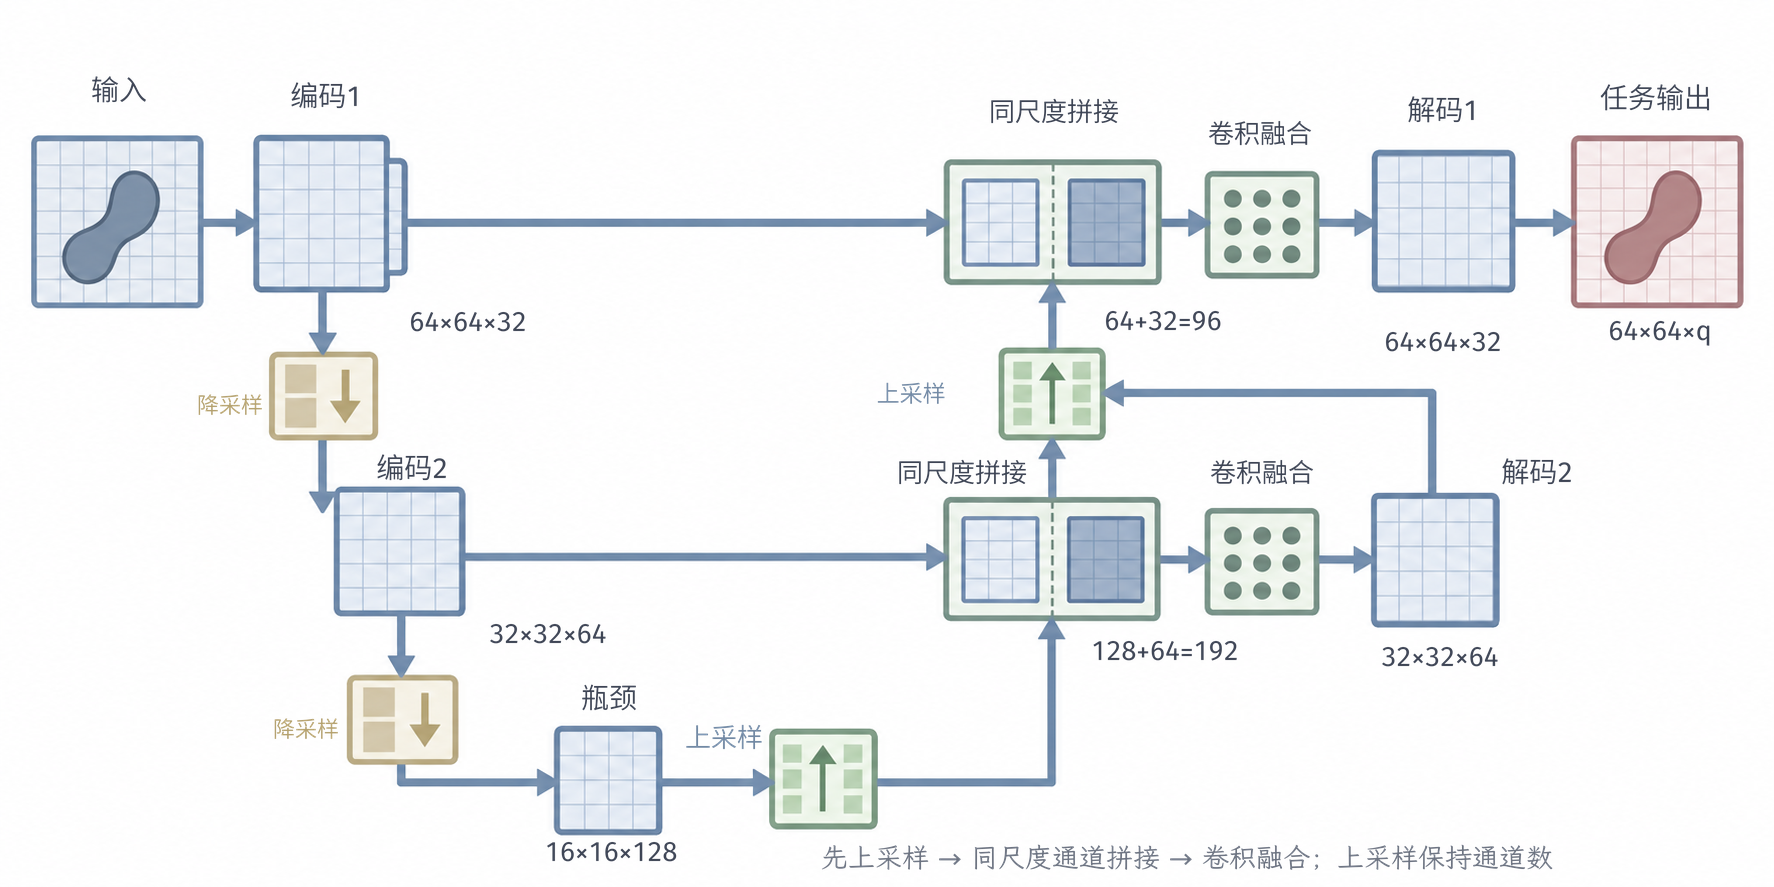
\includegraphics[width=150.199mm]{figures/03-models/02-neural-network-models/generated/cnn-encoder-decoder/figure.png}
  \caption{用于分割或着色的三尺度编码器—解码器。平面特征片表示特征张量，标签给出空间尺寸和通道数。每级解码先上采样到下一尺度，再在同尺度拼接框中沿通道合并编码特征，随后卷积融合；横向跳跃连接均接入拼接节点。图中上采样保持通道数，因此两次拼接分别得到$128+64=192$和$64+32=96$个通道，卷积后变为64和32个。输出头产生$q$个类别得分或两个颜色通道；采用same卷积，省略原始U-Net的裁剪。}
  \label{fig:cnn-encoder-decoder}
\end{figure*}

\term{上采样}（upsampling）是增加网格分辨率的操作。可以先用最近邻或双线性插值生成更密的网格，再用普通卷积处理；也可以用转置卷积共同完成位置扩展与可学习变换。插值方式、目标尺寸和坐标对齐约定都要固定。输入高、宽若不能被总下采样倍数整除，可以在进入网络前填充、在输出后裁剪，或显式按目标尺寸上采样；拼接还要求两个空间轴对齐。

训练时，每张图像提供像素标签，网络按式\eqref{eq:cnn-segmentation-loss}计算损失，再联合更新编码器、解码器和输出头。未标注位置通过掩码排除；若少数类别被大量背景像素淹没，可以在明确权重和归一化后使用加权损失。推理时不需要标签，在各位置取最大得分类别，得到与目标网格对齐的分割图。像素准确率可能主要反映背景，因此评价还需按任务检查区域重叠和边界质量，具体指标在图像处理部分展开。

跨尺度连接把编码器仍保存的细节送给解码器。小目标能否保留，取决于输入分辨率和下采样过程；预测边界的监督又来自标注质量。解码层数、损失和连接方式需要与这些信息来源共同配置。

\FloatBarrier

\subsection{图像生成}
\label{sec:cnn-colorization}

灰度图只提供亮暗信息，同样亮度的区域可以对应不同颜色。灰度图着色因此是一个\term{条件图像生成}（conditional image generation）问题：给定输入图像，生成与它相容的颜色图像。本节沿用编码器—解码器，展示如何形成空间输出；多个合理颜色之间的不确定性还需要由输出和目标来表达。

采用Lab颜色表示时，一个通道描述亮度，另外两个通道描述颜色差异。把亮度按固定规则归一化为输入$\bm X\in\mathbb R^{h\times w\times1}$，将训练彩色图的两个颜色通道按预定尺度变为目标$\bm C\in\mathbb R^{h\times w\times2}$。编码器读取亮度中的边缘、纹理和上下文，解码器恢复颜色的空间分布，最后用$1\times1$卷积输出两个通道。若目标被缩放到$[-1,1]$，可以在输出使用Tanh；采用线性输出时，则需在转换与显示环节处理范围。归一化常数、反归一化和颜色空间转换必须一致，转成RGB后还要处理显示色域。

最直接的教学模型产生确定的颜色估计$\widehat{\bm C}=\bm f_{\bm\theta}(\bm X)$，用像素平方损失训练：
\begin{equation}
  \ell_{\mathrm{col}}=\frac1{hw}\sum_{i=0}^{h-1}\sum_{j=0}^{w-1}
      \lVert\widehat{\bm C}_{i,j,:}-\bm C_{i,j,:}\rVert_2^2\text{。}
  \label{eq:cnn-colorization-loss}
\end{equation}
分割与着色的主体可以采用相同的空间结构，但分割在每个位置输出类别概率，着色在这里输出两个连续值。使用时，将预测颜色反归一化，与输入亮度组合，再转换成彩色图像；模型不应无意中改变输入与输出的空间对齐。

平方损失还有一个与任务有关的限制。在颜色具有有限二阶矩且预测函数可自由选择时，条件平方损失的最优预测是$\mathbb E[\bm C\mid\bm X]$。若同一个灰度输入可能对应多种相距较远的颜色，平均值未必是一种合理着色；例如红与绿的平均可能降低饱和度。Zhang等将颜色空间离散成候选颜色，预测每个位置的颜色分布，用分类目标保留这种多解性，并讨论了平方损失的平均效应\scite{zhang2016colorization}

若把输出头改为$q_{\mathrm{col}}$个颜色得分，就可以逐位置归一化为候选颜色概率，再按约定选择、平均或采样得到颜色。各位置分别归一化给出局部候选概率，整张图像的空间协调还依赖它们之间的联合关系。若希望对同一输入生成多个整体协调的结果，还需要引入随机变量并设计相应的分布学习目标。本节的确定性模型把亮度、上下文和颜色估计连接起来；完整的条件生成还要建模同一亮度输入下多种协调颜色之间的分布。

\Needspace{20\baselineskip}
\section{本章小结}
\label{sec:cnn-summary}

卷积网络对开篇问题给出了两项具体回答：局部连接把每次计算限定在邻域内，参数共享让同一组规则在不同位置重复使用。多通道组织保存不同的局部特征，非线性与层次组合使这些特征逐步参与更大范围的判断。网络是否保留空间轴、怎样处理边界和下采样，则决定了这种表示能否用于整体分类或逐位置输出。

计算算法规定如何得到卷积结果，工程实现规定怎样组织存储、访存与并行执行。直接计算、矩阵化和变换方法各有运算与数值代价，分块、展开和融合则改变数据复用与读写；二者需要结合层形状和平台选择。

数学卷积包含核翻转，网络常用互相关；填充、跨步、空洞和转置分别改变边界、窗口移动、核内采样与线性映射方向。明确这些约定，才能一致地计算输出形状、实现运算和推导梯度。参数共享使核梯度沿位置累积，窗口重叠使输入梯度累积。链式法则通过前向映射的转置，把输出梯度分配回输入，这一过程由导数关系确定。

跨层相加、门控与拼接改变了深层计算中的信息和梯度路径，也带来不同的通道规模与成本。这些路径参与训练中的求导与信息传递。预测可靠性还取决于结构是否保留目标所需信息、样本是否提供足够独立证据、参数与传播尺度是否受控，以及算法能否得到合适的解。分割与着色共同显示了这种配合：编码器构造上下文，解码器形成空间输出，跳跃连接保留细节，而输出头和损失决定最终预测究竟表示类别、连续值还是不确定性。

\paragraph{扩展阅读}
Goodfellow等教材第9章介绍卷积、共享和池化的结构假设；LeCun等的早期文档识别研究展示这些机制怎样配合实际任务。两项资料中，边界、步长与读出方式的配置展示了等变计算怎样转为任务输出，以及哪些位置细节在汇聚时被舍去\scite{goodfellow2016,lecun1998}

\chapter{循环神经网络}
\label{chap:recurrent-networks}

判断“这部电影并不精彩”的情感，需要把否定词与后面的评价相联系；预测设备下一时刻的温度，也常需要此前的升降趋势。第~\ref{chap:feedforward-networks}章说明了怎样把一个固定维度的输入变成预测，第~\ref{chap:convolutional-networks}章则利用局部邻域和参数共享处理规则网格。本章面对的问题是：输入陆续到达、序列长度可变时，网络怎样把历史中有用的信息带到当前，又怎样从当前的错误学会调整此前的处理？

隐状态是传递历史的内部表示，任务读出从中形成当前预测；训练再根据误差调整产生这些表示的参数。状态是否容纳了目标所需信息、损失能否影响相关更新，以及整段与逐步计算的代价，共同决定这种方法是否可用。普通循环网络先给出完整递推和学习过程，储备池、控制门、注意力与结构化状态更新再分别改变历史的构造、保存、读取和计算。拓扑与深度决定信息沿哪些路径传递，理论和应用据此考察求解条件与新序列上的预测。

\section{循环神经网络概述}
\label{sec:rnn-overview}

一种直接做法是把最近若干个观测拼成向量，交给前馈网络。这个窗口可以包含顺序，但窗口以外的信息不再参与预测；改变窗口长度还可能改变输入层的参数规模。时间卷积通过共享卷积核改善了这一点，但固定层数和核尺寸仍对应有限的感受野。若希望同一套计算持续处理新输入，就需要一个随着输入更新、能够传递历史影响的内部变量。

这个变量称为\term{隐状态}（hidden state）：它是网络根据已读输入形成的内部表示，不是训练样本直接提供的标签。设输入序列为$\bm{x}_1,\ldots,\bm{x}_T$，其中$\bm{x}_t\in\mathbb{R}^{d}$，长度$T$可以随样本改变。用$\bm{h}^{(t)}\in\mathbb{R}^{m}$表示读完第$t$个输入后的状态，\term{循环神经网络}（recurrent neural network, RNN）通过状态反馈，把前一步的内部表示用于下一步计算：
\begin{equation}
  \bm{h}^{(t)}=F_{\bm{\theta}}\!\left(\bm{h}^{(t-1)},\bm{x}_t\right),
  \qquad t=1,\ldots,T\text{。}
  \label{eq:rnn-general-recurrence}
\end{equation}
这里$F_{\bm{\theta}}$是具有参数$\bm{\theta}$的更新函数，$\bm{h}^{(0)}$是初始状态。下标$t$标识序列中的输入，上标$(t)$标识状态更新的步数；它们在本章按同一步对齐。状态的具体内容由更新函数和任务学习决定，可以是影响情感的否定，也可以是温度趋势；这条递推式只规定新状态从何处获得信息。

同一组$\bm{\theta}$在不同时间步复用，称为时间方向的\term{参数共享}（parameter sharing）。因此，延长序列会增加更新次数，却不必增加循环单元的参数量。\term{时间展开}（unrolling through time）则把这些更新依次画成计算图：第$t$步读取已经得到的第$t-1$步状态，展开图按已计算的旧状态逐步求值，形成有序的时间链。图~\ref{fig:rnn-unrolling}将状态反馈和展开图对应起来；展开后的深度随$T$增长，也是长序列训练困难的来源。

\begin{figure*}[htb]
  \centering
  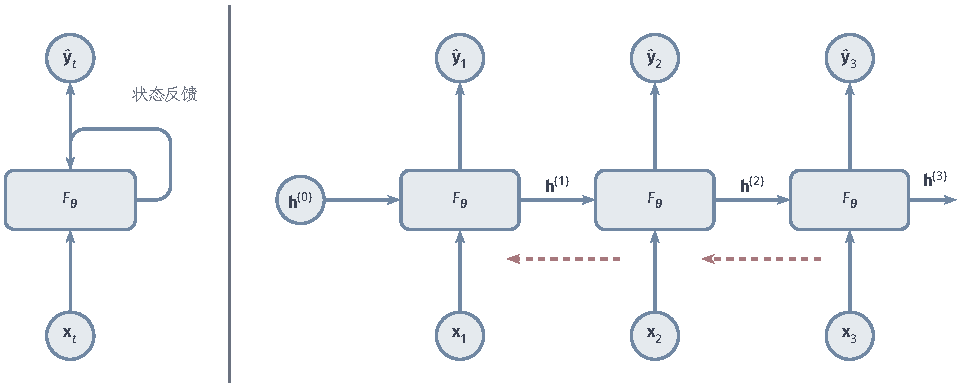
\includegraphics[width=162.810mm]{figures/03-models/02-neural-network-models/tikz/rnn-unrolling/figure.pdf}
  \caption{状态递推的紧凑表示与时间展开。当前输入进入更新函数，隐状态沿时间传递，任务读出从状态形成预测。展开图中的$F_{\bm{\theta}}$是同一个更新函数的多次调用，参数共享而状态值不同。红色虚线示意较晚损失沿状态依赖回传梯度；图中只画三个更新步。}
  \label{fig:rnn-unrolling}
\end{figure*}

循环网络的发展围绕两件事展开：怎样形成历史表示，以及怎样学到有用的状态更新。Elman在1990年的简单循环网络中，把前一步隐藏活动送回下一步，展示了这种上下文表示如何随序列任务形成。反馈在展开后成为一条时间链，同一参数因而可以作用于不同位置\scite{elman1990}

历史影响传到远处输出时，训练误差也要经过相应的多步依赖回传。Bengio、Simard和Frasconi在1994年分析了梯度学习与长期保留之间的困难：误差经多步状态变换回传时，影响可能迅速衰减或放大。这把研究重点从“网络是否含有反馈”推进到“反馈路径怎样传递信息与梯度”\scite{bengio1994rnn}

1997年的LSTM为持续记忆安排了单独的加性路径，后来加入的遗忘门使网络能够清除不再相关的内容。这条记忆通路与其他循环参数一起由任务目标训练。2001年的ESN和2002年的LSM则采用另一种分工：先构造通常固定的动态储备池，再学习任务读出。前一条路线让网络学习如何保存，后一条路线先提供历史特征；各自的原始工作和结构差别在第~\ref{sec:rnn-gated}节与第~\ref{sec:rnn-reservoir}节展开。

序列任务也推动了输出组织的变化。2014年，编码器—解码器使用一套循环网络读取源序列，另一套网络生成目标序列；Sutskever等用多层LSTM展示了这种端到端学习方式\scite{sutskever2014seq2seq} 同年的GRU用较少的门组织状态更新。随后，Bahdanau与Luong等的循环注意力模型让每个生成步骤重新读取编码器各位置的表示，减轻全部输入只能挤入同一末状态的限制。控制门改变保存方式，注意力改变读取方式，二者可以同时使用。

较新的状态空间路线还关心整段序列的计算组织。2020年的HiPPO把历史记忆写成在线投影问题；S4利用相应结构矩阵和快速核生成，在递推与卷积之间切换。2023年的Mamba把部分系数改为由输入产生，再通过选择性扫描计算；同年的RWKV以内容权重、时间衰减与定长累积量组织历史。第~\ref{sec:rnn-state-space}节将分别说明这些设计的原始形式。这些模型仍维护随输入更新的状态，并分别为状态构造、内容读取和计算执行安排结构。

本章按历史经由隐状态传递这一共同机制组织内容：链式循环、树递归、储备池以及基于隐状态递推的状态空间网络都在这里讨论。具体文献可能把状态空间网络单列为一类；各模型的具体更新函数和可训练参数在对应小节中另行给出。时间步也不必是物理时间，可以表示词的位置、扫描位置或有向结构中的计算次序。

\section{基础循环神经网络}
\label{sec:rnn-basic}

一个循环预测器包含状态更新、任务读出与损失三组计算。更新函数概括已读历史，读出规定在哪些位置形成什么预测，损失衡量预测与目标的差异。相同更新可以接末状态分类，也可以接逐位置预测；下面先建立这套共同计算。

\subsection{网络结构}
\label{sec:rnn-structure}

普通RNN把前一步状态和当前输入映射到同一个隐藏空间，再逐坐标使用非线性函数。采用列向量约定，令
\begin{equation}
  \begin{aligned}
    \bm{z}^{(t)}&=\bm{U}\bm{x}_t+\bm{W}\bm{h}^{(t-1)}+\bm{b},\\
    \bm{h}^{(t)}&=\tanh\!\left(\bm{z}^{(t)}\right),\\
    \bm{a}^{(t)}&=\bm{V}\bm{h}^{(t)}+\bm{c},\qquad
    \widehat{\bm{y}}_t=g\!\left(\bm{a}^{(t)}\right)\text{。}
  \end{aligned}
  \label{eq:rnn-basic-cell}
\end{equation}
其中$\bm{U}\in\mathbb{R}^{m\times d}$是输入映射，$\bm{W}\in\mathbb{R}^{m\times m}$是状态转移矩阵，$\bm{b}\in\mathbb{R}^{m}$是隐藏偏置；$\bm{V}\in\mathbb{R}^{q\times m}$和$\bm{c}\in\mathbb{R}^{q}$产生$q$维输出得分。$g$按任务选择恒等映射、Sigmoid或Softmax，输出与损失的配合沿用第~\ref{sec:ffn-output-objectives}节。Tanh可替换为其他激活，但梯度和状态范围会随之改变。

这个单元及读出共有$md+m^2+m+qm+q$个参数，忽略逐坐标运算后，一步稠密计算的乘加量为$O(md+m^2+qm)$。长度为$T$的前向计算重复$T$次。固定宽度时，逐步预测只需维护当前状态；完整反向传播还需要沿途激活，或在求导时重算它们；保存这些激活时，训练存储随展开长度增加。

\subsubsection{序列到分类}
\label{sec:rnn-sequence-classification}

如果一整段评论只对应一个情感标签，网络应在读完有效输入后输出一次。\term{序列到分类}（sequence classification）把长度可变的输入变成一个类别预测。最直接的读出使用末状态：
\begin{equation}
  \bm{p}=\operatorname{softmax}\!\left(\bm{V}\bm{h}^{(T)}+\bm{c}\right),
  \qquad \ell=-\log p_y\text{，}
  \label{eq:rnn-classification}
\end{equation}
其中类别数为$K$、$q=K$、真实标签为$y\in\{1,\ldots,K\}$。末状态必须把与类别有关的信息带到结尾，所以较早出现的证据也要经过后续更新。

另一种读出对状态聚合，例如用$\overline{\bm{h}}=T^{-1}\sum_{t=1}^{T}\bm{h}^{(t)}$替代末状态。这里聚合的是已含历史的状态，仍然可以体现顺序；但平均会稀释只出现在少数位置的证据。末状态集中保留递推后的历史，平均分散各位置的影响，最大池化突出局部强响应，可学习聚合则按目标调整权重。标签依赖哪些位置，决定了这些读出各自需要保留的证据。


图~\ref{fig:rnn-sequence-classification}显示了末状态分类的监督位置：只有读完有效序列后，分类头才形成整段预测。
\begin{figure}[htb]
  \centering
  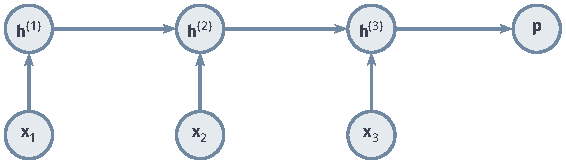
\includegraphics[width=95.793mm]{figures/03-models/02-neural-network-models/tikz/rnn-sequence-classification/figure.pdf}
  \caption{序列到分类。三个输入依次更新同一循环单元，末状态产生类别概率$\bm p$。输入、隐状态与任务输出分列展示；图中只示意长度为3的序列。}
  \label{fig:rnn-sequence-classification}
\end{figure}

\subsubsection{同步序列到序列}
\label{sec:rnn-aligned-sequences}

若每个词都要预测一个标签，输入位置与输出位置对齐。\term{同步序列到序列}（aligned sequence-to-sequence）在每个有效位置读出：
\begin{equation}
  \ell=\frac{1}{T}\sum_{t=1}^{T}
  \ell_t\!\left(g(\bm{V}\bm{h}^{(t)}+\bm{c}),y_t\right)\text{。}
  \label{eq:rnn-aligned-loss}
\end{equation}
单向状态$\bm{h}^{(t)}$只读取$\bm{x}_1,\ldots,\bm{x}_t$。实时预测可以按这个可见范围运行。若任务允许读取整段输入，可以使用第~\ref{sec:rnn-topologies}节的双向结构补充后文信息。

时间预测也可以按位置组织，但要注明输出的时间含义。例如读入$\bm{x}_t$后预测$\bm{x}_{t+1}$，计算索引仍是$t$，目标却是下一步观测。这里的对齐指每个输入位置都接一个预测；目标的物理时刻由任务另外指定。


图~\ref{fig:rnn-aligned-sequences}在各位置设置读出；它与末状态分类共享同一种状态递推，但各位置都可以收到监督。
\begin{figure}[htb]
  \centering
  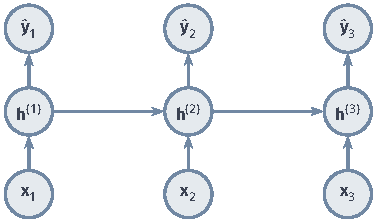
\includegraphics[width=63.793mm]{figures/03-models/02-neural-network-models/tikz/rnn-aligned-sequences/figure.pdf}
  \caption{同步序列到序列。每个输入位置形成一个隐状态和相应预测。输入位置与预测位置对齐；若用于下一时刻预测，应另将目标移到后一时刻。图中单向状态只读取当前及此前输入。}
  \label{fig:rnn-aligned-sequences}
\end{figure}

\subsubsection{异步序列到序列}
\label{sec:rnn-encoder-decoder}

把一段输入转换为另一段序列时，两者可能长度不同，也没有已知的逐位置对应。\term{编码器—解码器}（encoder--decoder）把读取输入和产生输出分成两套计算：编码器形成上下文，解码器以此为条件生成目标。设目标长度为$S$，目标符号来自大小为$K$的词表，约定词表包含起止符号BOS和EOS。

解码器要把离散符号转换成向量输入，因此为每个符号保存一个$d_e$维的可学习向量，并将它们排成嵌入矩阵$\bm{E}\in\mathbb{R}^{d_e\times K}$。若$y$是符号的词表索引，\term{符号嵌入}（symbol embedding）就是查表取出的那一列，即$\bm{e}(y)=\bm{E}_{:,y}$；索引只用于选列，其数值大小不表示符号间的距离。用$\bm{s}^{(j)}$表示解码状态，基本形式为
\begin{equation}
  \begin{aligned}
    \bm{c}_{\mathrm{enc}}&=\bm{h}^{(T)},\qquad
    \bm{s}^{(0)}=\psi(\bm{c}_{\mathrm{enc}}),\\
    \bm{s}^{(j)}&=F_{\mathrm{dec}}\!\left(
      \bm{s}^{(j-1)},\bm{e}(y_{j-1}),\bm{c}_{\mathrm{enc}}\right),\\
    \bm{p}^{(j)}&=\operatorname{softmax}\!\left(
      \bm{V}_{\mathrm{dec}}\bm{s}^{(j)}+\bm{b}_{\mathrm{dec}}\right)\text{。}
  \end{aligned}
  \label{eq:rnn-encoder-decoder}
\end{equation}
$\psi$将编码状态映射到解码状态空间，编码器与解码器可以使用不同参数和宽度。起始符号$y_0=\mathrm{BOS}$为第一步提供输入，终止符号$\mathrm{EOS}$表示生成结束；它们也有各自的嵌入列。下文把$y_S=\mathrm{EOS}$计入目标序列。使用真实前缀训练时，$y_{j-1}$来自目标序列；生成时，它来自上一步概率分布中选出或采样的符号。两种情况都先查表得到$\bm{e}(y_{j-1})$再输入解码器；概率分布用于产生符号，符号索引用于取嵌入列。嵌入矩阵与其他网络参数一起通过训练更新。

目标序列的条件概率按生成次序分解：
\begin{equation}
  \begin{aligned}
    p_{\bm{\theta}}(y_{1:S}\mid\bm{x}_{1:T})
      &=\prod_{j=1}^{S}p_{\bm{\theta}}
        (y_j\mid y_{0:j-1},\bm{x}_{1:T}),\\
    \ell&=-\sum_{j=1}^{S}\log p^{(j)}_{y_j}\text{。}
  \end{aligned}
  \label{eq:rnn-sequence-likelihood}
\end{equation}
这里$y_{1:S}$、$\bm{x}_{1:T}$简记相应序列。条件中保留了此前目标，所以概率分解没有假设目标位置互相独立。对损失求和或按$S$平均，会分别让长序列包含更多损失项或先把各序列归一化，因而改变样本权重。

图~\ref{fig:rnn-encoder-decoder}将读取源序列与生成目标分开。两侧各画三个有效位置以便比较，并不要求实际源序列与目标序列等长。
\begin{figure*}[t]
  \centering
  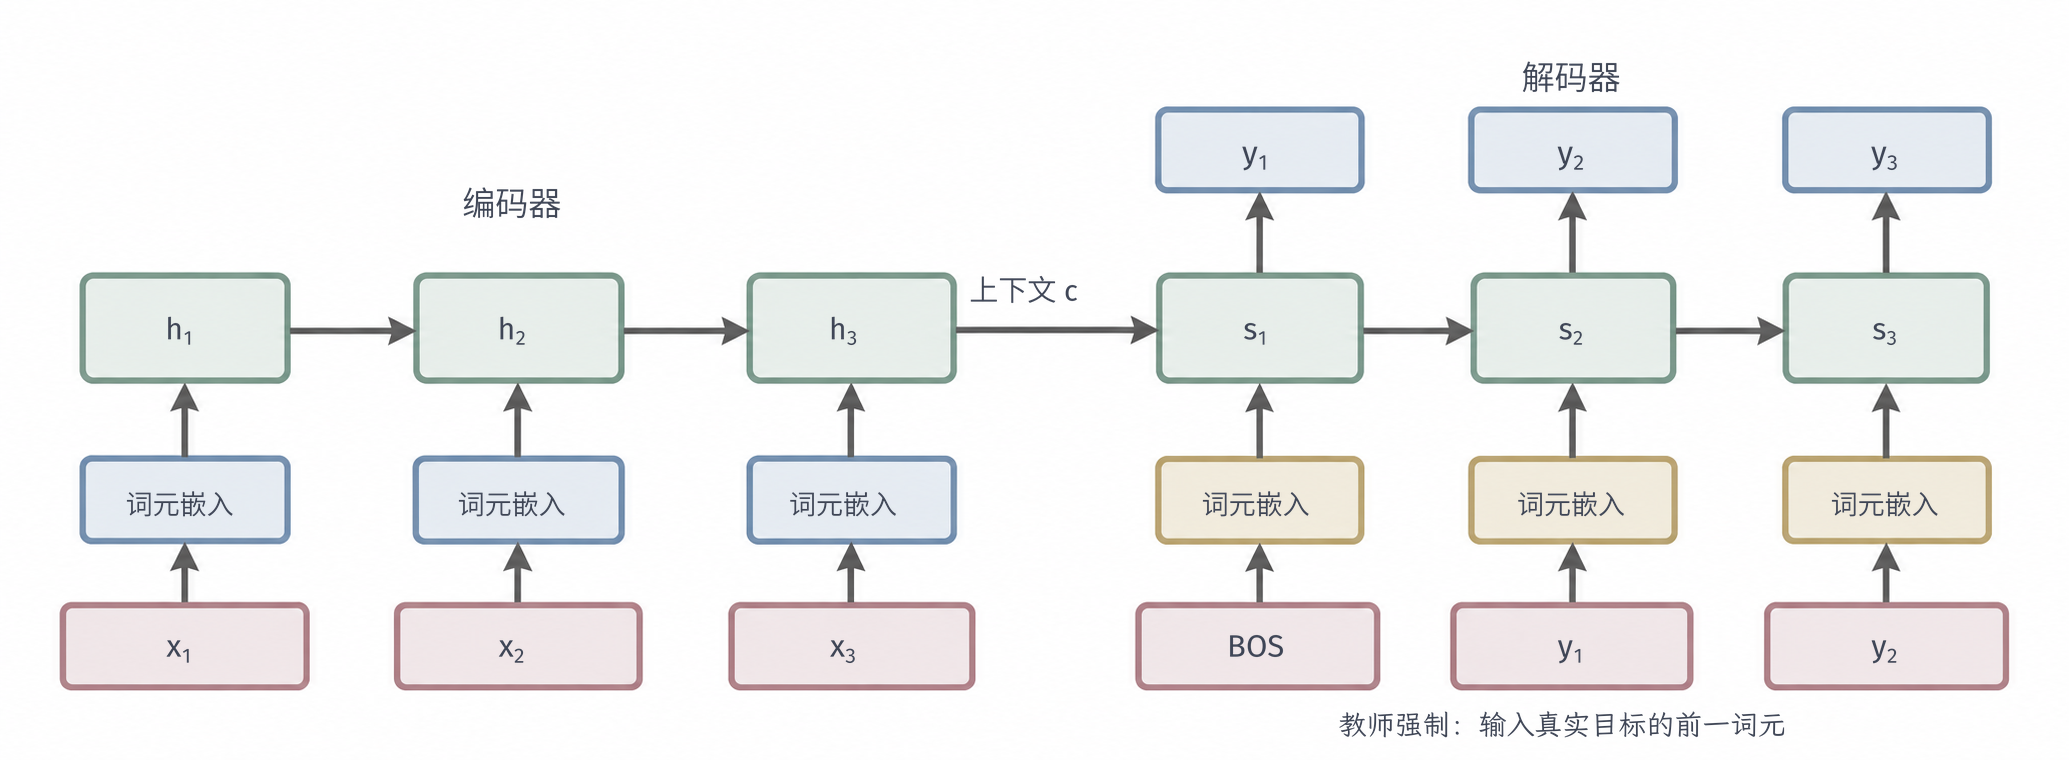
\includegraphics[width=169.000mm]{figures/03-models/02-neural-network-models/generated/rnn-encoder-decoder/figure.png}
  \caption{异步序列到序列。编码器读取三个源输入，解码器在初态$\bm s^{(0)}$之后生成三个目标。BOS启动生成，右移后的目标经嵌入进入后续解码步。训练可使用真实目标，预测使用已生成目标；图中省略每步重复读取的固定上下文。}
  \label{fig:rnn-encoder-decoder}
\end{figure*}

\subsection{参数学习}
\label{sec:rnn-learning}

每次更新都使用相同参数，训练必须把参数在不同时间步的影响加起来。输入和输出映射可沿用第~\ref{sec:ffn-initialization}节的尺度原则。循环矩阵会被重复使用，除了单步方差，还要关注多步乘积：正交初始化使初始线性变换保持欧氏范数，激活导数则继续参与完整状态的传播；两者共同决定起始梯度的尺度。

独立序列通常从零状态或同一个可学习的初始状态开始。若初始状态可学习，其梯度也由反向传播得到。连续数据流可以延续状态，但批次每一行延续同一条流时，状态才对应此前观测；换成无关样本时通过重置建立新预测条件。把上一个测试样本的状态带入下一个独立样本，会改变预测条件。

\subsubsection{随时间反向传播与共享梯度}
\label{sec:rnn-bptt}

把状态递推展开后，就能使用前馈网络的链式法则。\term{随时间反向传播}（backpropagation through time, BPTT）沿时间展开图从后向前计算导数。以下以式\eqref{eq:rnn-basic-cell}为对象，令单序列目标为$L=\sum_{t=1}^{T}\ell_t$；没有监督的位置取$\ell_t=0$。记$\bm{g}^{(t)}=\partial\ell_t/\partial\bm{a}^{(t)}$，总损失对状态的梯度为$\bm{r}^{(t)}$，对预激活的梯度为$\bm{\delta}^{(t)}$，则
\begin{equation}
  \begin{aligned}
    \bm{r}^{(t)}&=\bm{V}^{\top}\bm{g}^{(t)}
       +\bm{W}^{\top}\bm{\delta}^{(t+1)},\\
    \bm{\delta}^{(t)}&=\bm{r}^{(t)}\odot
      \left(\bm{1}-\bm{h}^{(t)}\odot\bm{h}^{(t)}\right),
      \qquad \bm{\delta}^{(T+1)}=\bm{0}\text{。}
  \end{aligned}
  \label{eq:rnn-backward-recursion}
\end{equation}
$\odot$表示逐元素乘法。第一项来自当前读出，第二项来自后续状态；即使当前没有标签，后续损失仍可通过第二项监督这一步。若只在末状态分类，$t<T$的$\bm{g}^{(t)}$均为零，但相应$\bm{\delta}^{(t)}$未必为零。

每次调用都对共享参数产生一个局部贡献。求这一局部贡献时，将该步读入的上一状态视为独立输入；跨步依赖已由$\bm{\delta}^{(t)}$汇总，当前局部外积据此只计算本次调用对参数的影响。把所有调用的贡献累积起来，得到
\begin{equation}
  \begin{aligned}
    \nabla_{\bm{U}}L&=\sum_{t=1}^{T}\bm{\delta}^{(t)}\bm{x}_t^{\top},
    &\nabla_{\bm{W}}L&=\sum_{t=1}^{T}\bm{\delta}^{(t)}
      (\bm{h}^{(t-1)})^{\top},\\
    \nabla_{\bm{b}}L&=\sum_{t=1}^{T}\bm{\delta}^{(t)},
    &\nabla_{\bm{V}}L&=\sum_{t=1}^{T}\bm{g}^{(t)}(\bm{h}^{(t)})^{\top},\\
    \nabla_{\bm{c}}L&=\sum_{t=1}^{T}\bm{g}^{(t)},
    &\nabla_{\bm{h}^{(0)}}L&=\bm{W}^{\top}\bm{\delta}^{(1)}\text{。}
  \end{aligned}
  \label{eq:rnn-shared-gradients}
\end{equation}
这些梯度的形状与相应参数一致。自动微分沿所有调用位置汇总导数；这些位置共用一组参数，各步贡献更新的是同一对象。若目标按时间平均，相应梯度还需除以有效长度。

\begin{figure}[htbp]
  \centering
  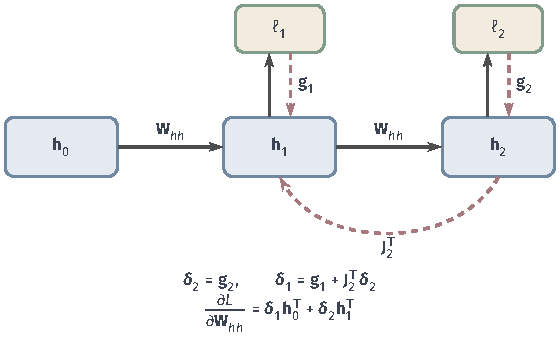
\includegraphics[width=94.756mm]{figures/03-models/02-neural-network-models/tikz/rnn-bptt-two-steps/figure.pdf}
  \caption{两时间步BPTT的显式展开。蓝色实线是共享$\bm W_{hh}$的前向调用，红色虚线从$\ell_2$与$\ell_1$回传并在$\bm\delta_1$处汇合；同一循环矩阵的梯度等于两个调用位置的外积贡献之和。底部指出长序列中状态Jacobian连乘是梯度消失或爆炸的直接来源。}
  \label{fig:rnn-bptt-two-steps}
\end{figure}

\begin{example}[两步递推中的梯度累积]
  \label{ex:rnn-shared-gradient}
  为单独观察共享参数，暂把Tanh换成恒等映射，使用标量更新$h^{(t)}=w h^{(t-1)}+x_t$；$w$是矩阵$\bm W$的一维情形。取固定初始状态$h^{(0)}=1$、$x_1=1$、$x_2=0$、$w=1/2$，只在末步计算损失$L=(h^{(2)})^2/2$。两次前向调用为
  \[
    \begin{aligned}
      h^{(1)}&=\tfrac12\times1+1=\tfrac32,\\
      h^{(2)}&=\tfrac12\times\tfrac32+0=\tfrac34\text{。}
    \end{aligned}
  \]
  反向从$r^{(2)}=h^{(2)}=3/4$开始，再沿第二步的状态依赖得到$r^{(1)}=w r^{(2)}=3/8$。本例激活导数为一，故$\delta^{(t)}=r^{(t)}$。第二次调用对$w$的局部导数是$h^{(1)}$，第一次是$h^{(0)}$，所以共享参数收到两项贡献：
  \[
    \begin{aligned}
      \frac{\mathrm dL}{\mathrm dw}
        &=r^{(1)}h^{(0)}+r^{(2)}h^{(1)}\\
        &=\tfrac38\times1+\tfrac34\times\tfrac32
          =\tfrac38+\tfrac98=\tfrac32\text{。}
    \end{aligned}
  \]
  第一项对应依赖路径$w\to h^{(1)}\to h^{(2)}\to L$，第二项对应$w\to h^{(2)}\to L$；梯度沿这些依赖逆向回传。两条路径的贡献最终相加，更新的仍是同一个$w$。直接展开$h^{(2)}=w(w+1)=w^2+w$，也有$\mathrm dL/\mathrm dw=(w^2+w)(2w+1)=3/2$，可与反向递推核对。

  若改取$h^{(0)}=0$，第一步对$w$的贡献为零，原因是$w$所乘的初态为零；共享参数仍在这一位置使用。若将本例的$h^{(0)}=1$改为可学习初态，它收到的梯度为$w r^{(1)}=3/16$，与$w$的梯度分开更新。
\end{example}

\subsubsection{截断、裁剪与状态管理}
\label{sec:rnn-truncation}

长序列的完整展开会占用大量训练存储。\term{截断随时间反向传播}（truncated BPTT）把数据流分成有限长度的片段，在片段边界保留状态数值，却切断对更早计算的求导依赖。保留的状态数值仍把此前历史带入当前预测，求导则仅经过当前片段的更新。截断缩小了反向图，前向记忆仍由递推动态决定；遗漏跨边界路径后，所得梯度通常是完整梯度的有偏近似。

梯度过大时，可以在优化器更新之前使用\term{梯度裁剪}（gradient clipping），把梯度范数限制在阈值内。将全部参数梯度拼成$\bm{g}$，阈值为$\tau>0$，全局范数裁剪写为
\begin{equation}
  \widetilde{\bm{g}}=
  \begin{cases}
    \bm{g},&\lVert\bm{g}\rVert_2\leq\tau,\\
    \tau\bm{g}/\lVert\bm{g}\rVert_2,&\lVert\bm{g}\rVert_2>\tau\text{。}
  \end{cases}
  \label{eq:rnn-gradient-clipping}
\end{equation}
它保持非零梯度的方向并限制步长尺度，可减少异常大梯度造成的更新幅度。裁剪作用于已算出的参数梯度，早期影响若已衰减仍需从传播路径处理，前向状态动态也保持原定义。Pascanu等从状态Jacobian矩阵的乘积分析这两类梯度问题，并研究了裁剪的作用\scite{pascanu2013}

可变长度批次常用填充补齐。\term{掩码}（mask）标记哪些位置是真实数据，使填充位置不参与损失或状态聚合。末状态读出使用每个样本的有效末位置；继续读取填充值会产生额外状态更新。平均聚合只汇聚有效位置，并以其数量作分母。

\subsubsection{教师强制与实际预测}
\label{sec:rnn-teacher-forcing}

式\eqref{eq:rnn-sequence-likelihood}计算的是给定真实前缀的条件概率。训练时把真实$y_{j-1}$作为第$j$步输入，称为\term{教师强制}（teacher forcing）：用正确前缀让模型学习下一符号的条件分布。预测时没有真实目标，只能反馈此前生成的符号。此前生成错误会改变后续状态，训练与预测遇到的前缀分布由此可能不同。

教师强制直接计算真实序列的条件似然。混合真实符号与模型生成符号后，训练所遇前缀和目标关系随之改变，要按新过程建立学习目标。生成质量由实际逐步预测过程中的输出评价。贪心解码每步选择概率最大的符号；束搜索保留多个候选前缀，保留下来的候选只覆盖搜索空间的一部分，完整序列的选择受到束宽限制。

\subsubsection{长期依赖问题及解决思路}
\label{sec:rnn-long-dependencies}

较早的输入能否影响很晚的输出，取决于这种影响经过多次更新后还剩多少。\term{长期依赖}（long-term dependency）指当前任务需要利用相距很多步的信息；相隔多少步算长，要相对于任务和模型的有效记忆尺度判断。

固定输入序列，记一步更新的状态\term{Jacobian矩阵}为$\bm{J}^{(t)}=\partial\bm{h}^{(t)}/\partial\bm{h}^{(t-1)}$，沿用卷一的行输出、列输入约定。它描述前一步状态的小变化如何影响后一步。链式法则给出
\begin{equation}
  \frac{\partial\bm{h}^{(t)}}{\partial\bm{h}^{(s)}}
    =\bm{J}^{(t)}\bm{J}^{(t-1)}\cdots\bm{J}^{(s+1)},
    \qquad t>s\text{。}
  \label{eq:rnn-jacobian-product}
\end{equation}
前向的状态敏感度使用这个乘积，反向的损失梯度使用其转置。普通Tanh单元中，$\bm{J}^{(t)}=\bm{D}^{(t)}\bm{W}$，$\bm{D}^{(t)}$的对角元素为$1-(h_i^{(t)})^2$。多步传播因此同时包含$\bm{W}$的线性作用、激活导数，以及不同步矩阵的相乘顺序。

若所有相关步都有$\lVert\bm{J}^{(t)}\rVert_2\leq r<1$，则乘积范数不超过$r^{t-s}$，早期扰动与沿这条路径回传的梯度都受到指数衰减的上界。\term{梯度消失}（vanishing gradients）使早期参数难以收到有效更新。若某些方向在多步乘积中持续放大，则可能出现\term{梯度爆炸}（exploding gradients）。单步范数描述最强放大方向，多步中实际方向还会变化；矩阵方向、激活饱和与输入共同决定沿具体轨迹的乘积。

\begin{example}[传播距离与状态保留]
  \label{ex:rnn-memory-decay}
  对线性标量递推$h^{(t)}=a h^{(t-1)}+x_t$，若$x_1=1$、后续输入为零且$h^{(0)}=0$，则$h^{(T)}=a^{T-1}$，跨步敏感度也为$a^{T-1}$。取$T=101$，$a=0.9$时为约$2.66\times10^{-5}$，$a=1.1$时为约$1.38\times10^4$。取$a=1$时，这个单一信号一直保留，多个输入则累加到同一状态中；任务读出还需要从累积结果区分所需历史。
\end{example}

式\eqref{eq:rnn-jacobian-product}包含两类因素：一条依赖路径经过多少次变换，以及每次变换怎样放大或衰减。控制路径长度与控制逐步增益，由此成为不同的结构设计。对一条含$\nu$次状态变换的路径，若各步范数不超过$r$，则
\begin{equation}
  \left\lVert\bm J_{\nu}\cdots\bm J_1\right\rVert_2
    \leq\prod_{k=1}^{\nu}\lVert\bm J_k\rVert_2\leq r^{\nu}\text{。}
  \label{eq:rnn-path-length-rate}
\end{equation}
$r$控制逐步变化的尺度，$\nu$控制这种变化重复多少次。这个范数上界控制路径上的最大放大程度；下面据此分别考察逐步增益、路径长度和内容选择。

\subsubsection{参数约束：控制逐步放大与衰减}
\label{sec:rnn-parameter-constraints}

若传播方向的增益长期大于1，限制状态变换的范数可以减小指数放大；若增益长期小于1，只把范数压得更小反而会加重消失。保存长期影响需要相关方向的传播系数接近1，同时限制异常放大的方向。逐步增益的约束要同时满足这两类要求。

更强的条件同时约束最大和最小奇异值。若各步状态Jacobian矩阵的奇异值均在$[q,r]$内，$q>0$，对任意末端梯度$\bm v$有
\begin{equation}
  q^{\nu}\lVert\bm v\rVert_2
    \leq\left\lVert(\bm J_{\nu}\cdots\bm J_1)^{\top}\bm v\right\rVert_2
    \leq r^{\nu}\lVert\bm v\rVert_2\text{。}
  \label{eq:rnn-path-singular-bounds}
\end{equation}
使$q$与$r$都接近1，才同时抑制过快衰减与过快放大。普通Tanh单元的$\bm J^{(t)}=\bm D^{(t)}\bm W$还包含激活导数：即使约束$\bm W^{\top}\bm W=\bm I$，饱和的Tanh仍可使$\bm D^{(t)}$接近零。正交或酉矩阵约束保护的是线性部分，必须配合激活、输入尺度和完整Jacobian矩阵分析\scite{arjovsky2016unitary}

固定储备池是对可训练参数施加更强约束的一种做法。把循环动态参数$\bm\theta_{\mathrm{res}}$固定为$\bm\theta_0$，相当于将其可行集合限制为单点$\{\bm\theta_0\}$，任务训练只优化读出参数。储备池构造还常限制循环矩阵的尺度、连接和泄漏率，以安排状态的稳定性和记忆时间尺度。

冻结参数只限定训练的优化范围；前向动态的衰减或放大仍由这组固定参数决定。固定储备池的另一项作用，是训练时不再需要把末端错误沿长时间链传回循环参数，读出只需利用已经生成的状态特征。长距离任务梯度因此只需训练读出；任务相关历史是否到达读出，仍由固定动态提供的状态特征决定。

\subsubsection{跨时间跳跃：减少一条路径的变换次数}
\label{sec:rnn-temporal-skips}

另一种做法增加从较早状态直接到较晚状态的边，例如
\begin{equation}
  \bm h^{(t)}=F_{\bm\theta}(\bm h^{(t-1)},\bm x_t)
       +\bm S\bm h^{(t-k)},\qquad t\geq k\text{，}
  \label{eq:rnn-temporal-skip}
\end{equation}
其中$k$是跳跃间隔，$\bm S\in\mathbb R^{m\times m}$是直达映射，边界状态另行初始化。从$t-k$到$t$的直接路径只经过$\bm S$。跨越距离$pk$时，沿连续跳跃边的一条路径经过$p$次变换；在$\lVert\bm S\rVert_2\leq r$下，该路径的范数上界为$r^p$，普通逐步路径则可能含$pk$次变换。

在标量教学例子中，同样以$0.9$为路径系数，跨100步的逐步路径为$0.9^{100}\approx2.66\times10^{-5}$，每10步跳一次的路径为$0.9^{10}\approx0.349$。这是新增路径的比较；完整梯度包含所有路径贡献的和，单一路径的$r^{\nu/k}$只是其中的传播尺度。跳跃也需要保存相应旧状态，并可能跳过任务所需的细粒度处理。

跨层残差改变层方向路径，跨时间跳跃改变时间方向依赖。直达路径之外，其他分支和多路径相加也参与梯度；状态中的目标信息还需要由读出提取。

\subsubsection{控制门：让保留率随内容改变}
\label{sec:rnn-gated-memory-path}

固定约束对所有输入使用同一规则，任务却可能只需保存某些内容。控制门把保留系数变成输入相关量。以LSTM的直接记忆路径为例，暂固定门的数值后，从$s$到$t$的逐坐标系数为$\prod_{u=s+1}^{t}f_i^{(u)}$。需要保存时令相应遗忘门接近1，需要覆盖时降低它；输入门再调节新内容写入。门控主要改变逐步保留率与信息通路，通常没有减少时间步数。

门本身也依赖状态，完整Jacobian矩阵还包含门与候选变化的路径。能建立接近恒等的记忆通路，为训练提供了选择，任务损失仍需学到何时使用它。第~\ref{sec:rnn-lstm}节和第~\ref{sec:rnn-gru}节将把这些路径写成具体单元。

这几类方式可以组合：固定储备池也能加入跳跃连接，门控网络也能约束部分矩阵。传播路径、逐步增益、可训练参数范围和读出所需信息，分别描述这些组合实际改变了什么。

\section{基于储备池的循环神经网络}
\label{sec:rnn-reservoir}

如果难点在于学习复杂的循环动态，可以把构造动态与学习任务输出分开。\term{储备池计算}（reservoir computing）用一个通常固定的动态系统把输入历史转换成丰富状态，再学习从状态到目标的读出。这里的\term{读出}（readout）是任务输出映射：它接收状态特征，计算回归值或类别概率。状态随输入改变，但产生状态的循环参数通常不按当前任务的梯度更新。图~\ref{fig:rnn-reservoir}展示了这一分工。

\begin{figure*}[htb]
  \centering
  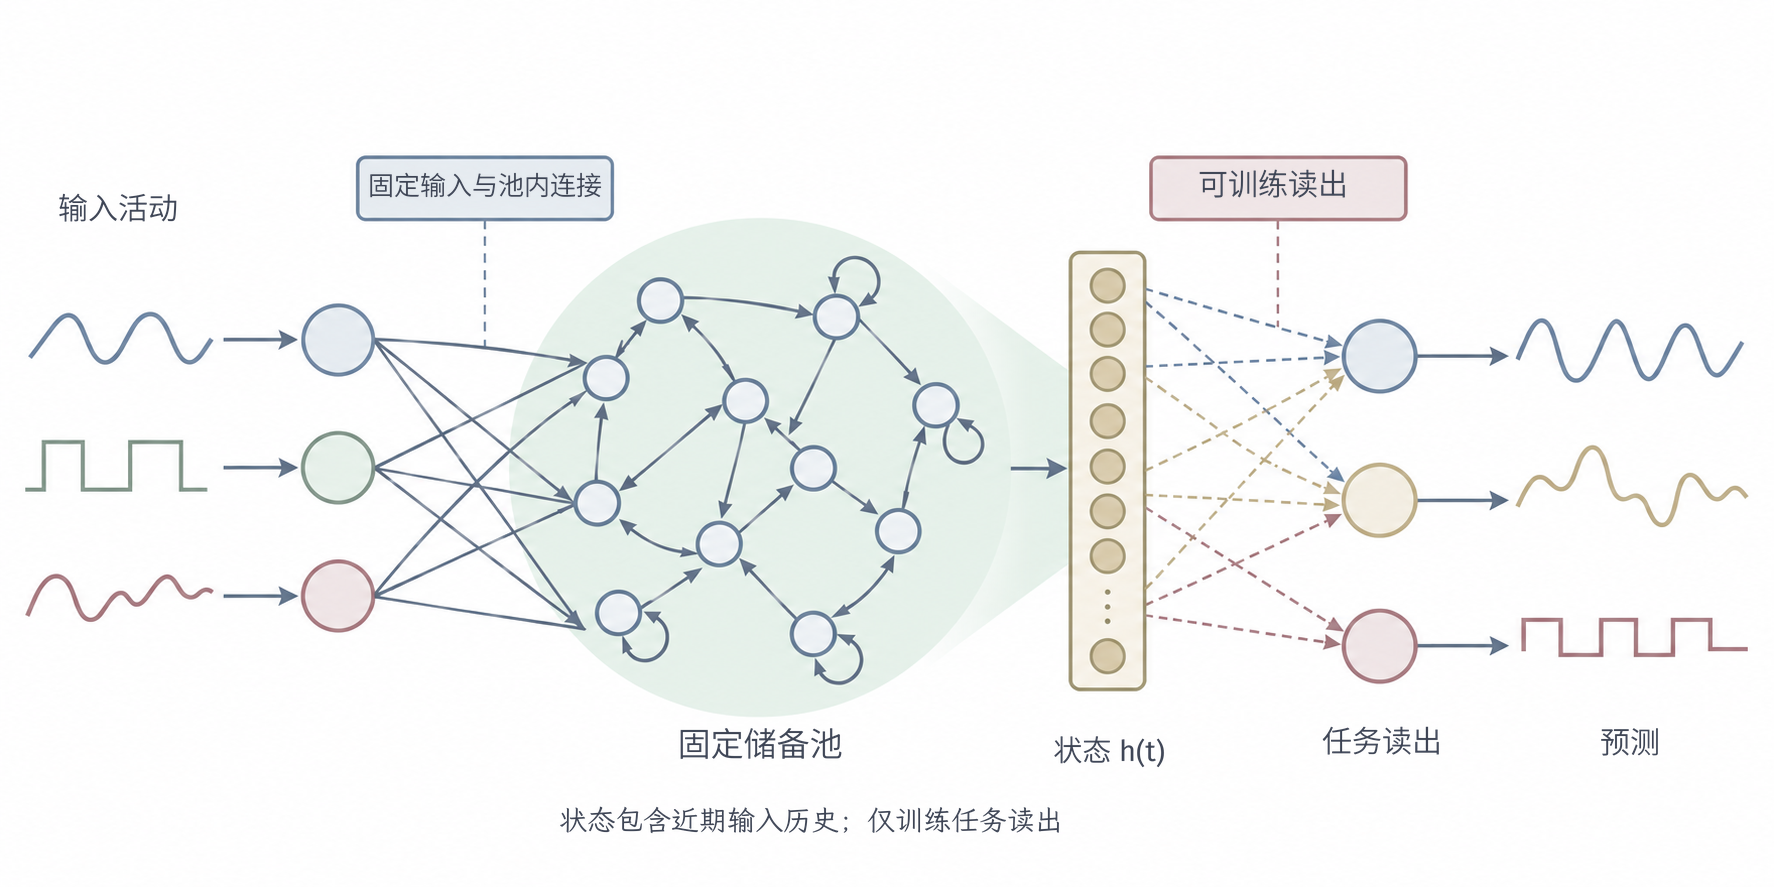
\includegraphics[width=150.199mm]{figures/03-models/02-neural-network-models/generated/rnn-reservoir/figure.png}
  \caption{储备池计算的参数分工。输入进入固定的循环动态，多个内部单元共同形成随历史变化的状态，可训练读出将状态映射到目标。灰色连线表示固定连接，箭头表示参与拟合的读出；内部连接只示意结构，不表示某个随机生成样本。ESN使用连续值激活，LSM可由脉冲活动及其滤波响应形成读出特征。}
  \label{fig:rnn-reservoir}
\end{figure*}

\subsection{ESN}
\label{sec:rnn-esn}

\term{回声状态网络}（echo state network, ESN）是一种以连续值循环状态提供历史特征的储备池模型，Jaeger的技术报告建立了其基本框架\scite{jaeger2001} 下面采用无输出反馈的泄漏积分版本，避免把真实目标或读出结果再送入储备池。令泄漏率$\alpha\in(0,1]$，更新为
\begin{equation}
  \begin{aligned}
    \widetilde{\bm{h}}^{(t)}&=\tanh\!\left(
      \bm{W}_{\mathrm{res}}\bm{h}^{(t-1)}
      +\bm{U}_{\mathrm{res}}\bm{x}_t+\bm{b}_{\mathrm{res}}\right),\\
    \bm{h}^{(t)}&=(1-\alpha)\bm{h}^{(t-1)}
       +\alpha\widetilde{\bm{h}}^{(t)}\text{。}
  \end{aligned}
  \label{eq:rnn-esn-update}
\end{equation}
$\bm{W}_{\mathrm{res}}\in\mathbb{R}^{m\times m}$、$\bm{U}_{\mathrm{res}}\in\mathbb{R}^{m\times d}$和偏置通常构造后固定。较小$\alpha$使每次状态变化较慢，但实际记忆还取决于循环矩阵、输入尺度和非线性响应。稀疏连接、输入缩放、泄漏率和状态维度均是可由验证选择的配置。

训练时先运行储备池，收集特征$\bm{z}_t=[1;\bm{x}_t;\bm{h}^{(t)}]\in\mathbb{R}^{1+d+m}$，分号表示向量拼接。初始若干步可能主要反映人为初态，常丢弃这段\term{洗出期}（washout），即先让系统接受输入、再开始拟合读出。洗出期剔除的是受初态影响的读出特征，任务标签所依赖的输入仍要进入状态更新；独立序列采用一致的洗出和重置规则。

对连续值目标，将$N$个有效状态按行堆成$\bm{Z}\in\mathbb{R}^{N\times(1+d+m)}$，相应目标堆成$\bm{Y}\in\mathbb{R}^{N\times q}$。线性读出参数为$\bm{R}\in\mathbb{R}^{(1+d+m)\times q}$，采用平方损失和岭惩罚时
\begin{equation}
  \begin{aligned}
    \bm{R}^{\star}&=\argmin_{\bm{R}}
      \lVert\bm{Z}\bm{R}-\bm{Y}\rVert_{\mathrm{F}}^2
      +\lambda\lVert\bm{R}\rVert_{\mathrm{F}}^2,\\
    \bm{R}^{\star}&=(\bm{Z}^{\top}\bm{Z}+\lambda\bm{I})^{-1}
      \bm{Z}^{\top}\bm{Y},\qquad \lambda>0\text{。}
  \end{aligned}
  \label{eq:rnn-esn-ridge}
\end{equation}
这里$\lVert\cdot\rVert_{\mathrm{F}}$是Frobenius范数。公式惩罚了包括截距在内的全部系数；若不惩罚截距，应改用相应对角惩罚矩阵并另查可逆性。实现时可解对应线性方程，公式中的逆矩阵表示其解。Softmax与交叉熵读出则产生另一种目标，按分类目标训练参数。

任务读出希望状态主要由输入历史决定，初态差异随持续输入逐渐减弱。\term{回声状态性质}（echo state property, ESP）要求在约定的输入与状态范围内，相同持续输入驱动下，初始状态的影响最终消失。对式\eqref{eq:rnn-esn-update}，Tanh是1-Lipschitz，因而两个状态的距离满足
\begin{equation}
  \lVert\bm{h}^{(t)}-\bm{h}_{\mathrm{alt}}^{(t)}\rVert_2
    \leq\left(1-\alpha+\alpha\lVert\bm{W}_{\mathrm{res}}\rVert_2\right)
      \lVert\bm{h}^{(t-1)}-\bm{h}_{\mathrm{alt}}^{(t-1)}\rVert_2\text{。}
  \label{eq:rnn-esn-contraction}
\end{equation}
这里$\bm{h}^{(t)}$与$\bm{h}_{\mathrm{alt}}^{(t)}$表示初态不同、输入相同的两条轨迹。$\lVert\bm{W}_{\mathrm{res}}\rVert_2<1$给出统一收缩的充分条件，但不是必要条件。按谱半径缩放限制线性模式，非线性储备池还包含激活和输入驱动；相关反例与更精确条件见Yildiz等的分析\scite{yildiz2012}

初态影响消失也意味着一部分过去影响会衰减，适当的衰减使模型能适应新输入，过快衰减却可能丢掉任务证据。\term{记忆容量}（memory capacity）的一种线性测量方法，是对独立同分布的零均值标量输入分别学习各延迟的线性重构，再累加平方相关系数。在状态为$m$维、读出仅使用状态且采用相应总体最小二乘定义的条件下，总线性记忆容量不超过$m$；这项容量指标衡量线性延迟重构，任务分类的准确率由相应目标另外评价\scite{jaeger2001memory} 读出优化利用已有特征，远期证据是否仍可区分则要从动态状态检验。

\subsection{LSM}
\label{sec:rnn-lsm}

输入也可能由带时间戳的事件构成，如传感器事件或神经脉冲。\term{液态状态机}（liquid state machine, LSM）用动态储备池的瞬时响应表示输入历史，代表性实现是固定的脉冲神经元回路，再学习状态读出。其名称强调利用持续变化的内部活动，不要求系统每次都收敛到一个稳定状态。

图~\ref{fig:rnn-lsm}把输入到任务输出的过程分开。输入是事件时，可以直接接入脉冲回路；连续观测则需按约定编码为输入脉冲。编码规则决定观测幅度、变化或时间如何转成回路接受的事件输入。
\begin{figure*}[htb]
  \centering
  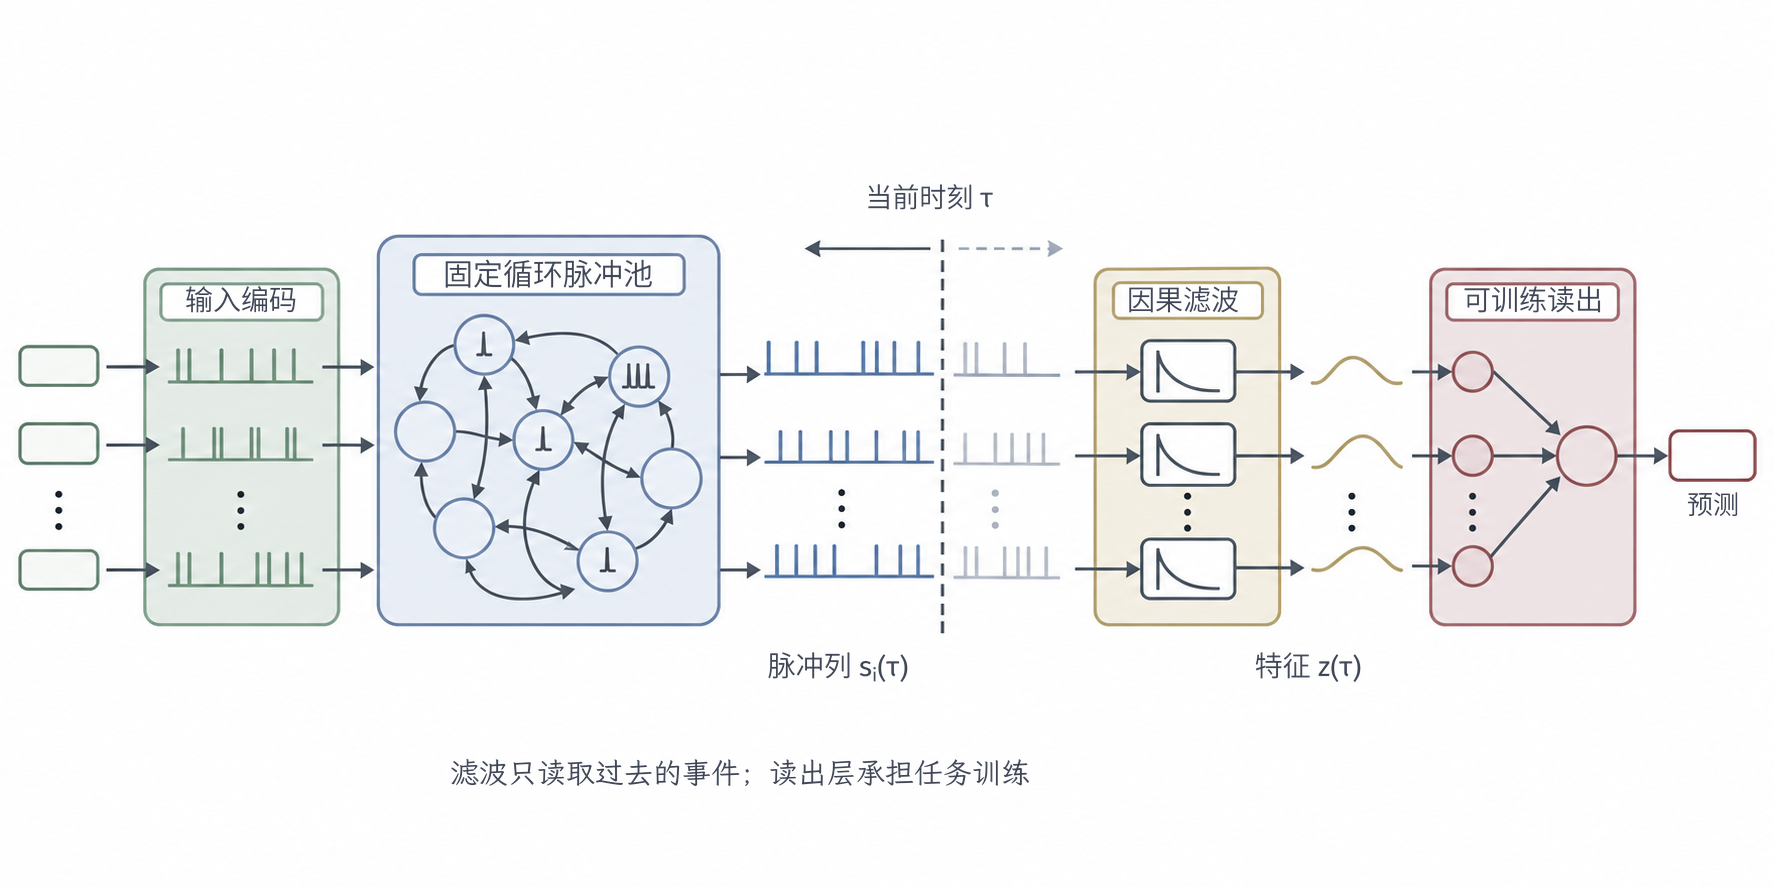
\includegraphics[width=150.199mm]{figures/03-models/02-neural-network-models/generated/rnn-lsm/figure.png}
  \caption{LSM的输入、动态与读出。输入编码驱动固定的循环脉冲储备池，回路活动形成脉冲列$s_i(\tau)$；因果滤波将这些活动变成当前可读特征$\bm z(\tau)$，任务读出再映射为预测。反馈表示回路动态，滤波后的特征进入可训练任务读出。此处只训练任务读出，脉冲编码、回路参数与滤波核按约定固定。}
  \label{fig:rnn-lsm}
\end{figure*}

回路中的状态比“这个时刻是否发出脉冲”更丰富。例如一个简化的漏积分发放单元可以写为
\begin{equation}
  \tau_{\mathrm m}\frac{\mathrm d v_i(\tau)}{\mathrm d\tau}
    =-(v_i(\tau)-v_{\mathrm{rest}})
      +I_i(\tau)+\sum_j w_{i,j}(\kappa_{\mathrm{syn}}*s_j)(\tau)\text{，}
  \label{eq:rnn-lsm-membrane}
\end{equation}
其中$v_i$是膜电位，$\tau_{\mathrm m}>0$是泄漏时间常数，$I_i$表示换算到同一电位尺度的外部驱动，$w_{i,j}$是固定连接权重，$\kappa_{\mathrm{syn}}*s_j$是此前脉冲经过突触滤波后的作用。膜电位达到阈值时发出脉冲并重置；这里省略不应期等细节。持续的膜电位、突触响应和反馈活动共同承载输入历史，当前输入停止后，内部影响仍可能延续\scite{maass2002}

若第$i$个单元在时刻$\tau_{i,k}$发出脉冲，其脉冲列为$s_i(\tau)=\sum_k\delta(\tau-\tau_{i,k})$，$\delta$是Dirac脉冲。它不是某一时刻的普通有限函数值，而是用积分记录一次单位事件：与连续权重函数相乘后积分，就取出该函数在发放时刻的值。因而可以用因果滤波核$\kappa_i$形成特征：
\begin{equation}
  z_i(\tau)=\int_{-\infty}^{\tau}\kappa_i(\tau-u)s_i(u)\,\mathrm du,
  \qquad \kappa_i(v)=e^{-v/\tau_i}\mathbf 1_{\{v\geq0\}}\text{。}
  \label{eq:rnn-lsm-filter}
\end{equation}
$\tau_i>0$是特征衰减时间常数，$\mathbf 1$是指示函数。采用事件发生后立即计入当前状态的约定，积分可以逐个发放时刻展开为
\begin{equation}
  z_i(\tau)=\sum_{k:\,\tau_{i,k}\leq\tau}
    \exp\!\left(-\frac{\tau-\tau_{i,k}}{\tau_i}\right)\text{。}
  \label{eq:rnn-lsm-event-sum}
\end{equation}
每次脉冲向$z_i$加入$1$，此后按已经过去的时间衰减；未来事件不参与求和。脉冲编码的进一步说明见第~\ref{sec:snn-coding}节。这一步是状态读取：把回路活动整理成有限维、可供后续计算的$\bm z(\tau)$。这些滤波特征保留了所选脉冲响应，膜电位和其他突触变量仍可能未被记录；读出获得的信息范围由所选特征决定。

读出是从这些状态特征到任务预测的映射，作用相当于前馈网络的输出头。读取特征与产生任务答案是两步计算；一个常用读出为
\begin{equation}
  \bm a(\tau)=\bm V\bm z(\tau)+\bm b,
  \qquad\widehat{\bm y}(\tau)=g(\bm a(\tau))\text{，}
  \label{eq:rnn-lsm-readout}
\end{equation}
其中$\bm z\in\mathbb R^m$、$\bm V\in\mathbb R^{q\times m}$。回归可取$g$为恒等映射，分类可取Sigmoid或Softmax；训练样本提供目标，监督$\bm V,\bm b$的学习。读出也可以是更复杂的可训练网络，两种历史若产生相同的$\bm z$，只读取$\bm z$的确定性读出就给出相同结果，因而特征本身也要保留任务所需区别。

\begin{example}[从脉冲活动到预测]
  \label{ex:rnn-lsm-readout}
  假设两个单元均使用时间常数2：第一个在时刻1和3发放，第二个只在时刻2发放。在时刻4，特征为$z_1=e^{-3/2}+e^{-1/2}\approx0.830$、$z_2=e^{-1}\approx0.368$。若教学例子中的回归读出为$\widehat y=2z_1-z_2-0.5$，便得到约$0.791$。脉冲与滤波决定特征，系数$(2,-1)$和偏置决定这些特征怎样形成任务答案；训练用状态特征及对应目标估计读出系数和偏置。
\end{example}

训练时先按实际顺序驱动回路，在约定时刻收集状态特征及对应目标，再拟合读出。平方损失的线性读出可沿用ESN的岭回归，分类读出则使用相应分类目标。独立事件序列需要重置或约定初态，同一连续流可以延续状态；采集特征时仍须遵守预测时的信息范围。

LSM对长期依赖的帮助来自动态特征的时间范围：较慢的突触／滤波响应保留较久的影响，循环反馈还可延长或重组这种影响。过快的衰减会丢掉远期证据，过强反馈可能使无关活动持续，多个历史也可能被压成相同特征。固定回路减少了训练循环参数的困难，但读出能否利用长期历史，取决于特征是否仍可区分任务所需的历史。

ESN主要以连续值激活表示状态，LSM利用脉冲时刻及其动态响应。事件稀疏时可采用事件驱动计算，数字仿真的更新、通信和读出成本仍需计入。脉冲编码、膜电位模型与可塑性学习在后续脉冲神经网络章展开，这里的动态负责提供历史表示，监督训练负责把这些表示转换成任务预测。

\section{基于控制门的循环神经网络}
\label{sec:rnn-gated}

固定动态难以针对任务选择性地保留信息，普通RNN又把已有状态和新输入混合后整体变换。\term{控制门}（gate）是由输入和状态计算的一组系数，用逐元素乘法调节哪些信息保留、写入或输出。Sigmoid将系数限制到$(0,1)$，使门可以连续学习。门的参数与其他网络参数一起根据最终任务损失更新，保留和写入行为因而可以随任务形成。

\subsection{LSTM}
\label{sec:rnn-lstm}

\term{长短期记忆}（long short-term memory, LSTM）把持续保存的记忆和对外输出的隐藏表示分开，通过门调节二者。原始LSTM发表于1997年，常见的遗忘门后来加入；以下讲解带遗忘门、无窥孔连接的常用版本\scite{hochreiter1997}

令$\bm{c}^{(t)}\in\mathbb{R}^{m}$是记忆状态，$\bm{h}^{(t)}\in\mathbb{R}^{m}$是隐藏输出。门均读取$[\bm{x}_t;\bm{h}^{(t-1)}]\in\mathbb{R}^{d+m}$，计算
\begin{equation}
  \begin{aligned}
    \bm{i}^{(t)}&=\operatorname{sigmoid}\!\left(
      \bm{A}_{\mathrm{i}}[\bm{x}_t;\bm{h}^{(t-1)}]+\bm{b}_{\mathrm{i}}\right),\\
    \bm{f}^{(t)}&=\operatorname{sigmoid}\!\left(
      \bm{A}_{\mathrm{f}}[\bm{x}_t;\bm{h}^{(t-1)}]+\bm{b}_{\mathrm{f}}\right),\\
    \bm{o}^{(t)}&=\operatorname{sigmoid}\!\left(
      \bm{A}_{\mathrm{o}}[\bm{x}_t;\bm{h}^{(t-1)}]+\bm{b}_{\mathrm{o}}\right),\\
    \widetilde{\bm{c}}^{(t)}&=\tanh\!\left(
      \bm{A}_{\mathrm{c}}[\bm{x}_t;\bm{h}^{(t-1)}]+\bm{b}_{\mathrm{c}}\right)\text{。}
  \end{aligned}
  \label{eq:rnn-lstm-gates}
\end{equation}
每个$\bm{A}$属于$\mathbb{R}^{m\times(d+m)}$，每个偏置属于$\mathbb{R}^{m}$。输入门$\bm{i}^{(t)}$决定候选记忆写入多少，遗忘门$\bm{f}^{(t)}$决定旧记忆保留多少，输出门$\bm{o}^{(t)}$决定记忆的变换结果读出多少：
\begin{equation}
  \begin{aligned}
    \bm{c}^{(t)}&=\bm{f}^{(t)}\odot\bm{c}^{(t-1)}
       +\bm{i}^{(t)}\odot\widetilde{\bm{c}}^{(t)},\\
    \bm{h}^{(t)}&=\bm{o}^{(t)}\odot\tanh\!\left(\bm{c}^{(t)}\right)\text{。}
  \end{aligned}
  \label{eq:rnn-lstm-update}
\end{equation}
遗忘门值接近1时保留旧记忆，接近0时清除相应坐标。新旧信息在记忆路径上相加，隐藏输出则经过Tanh和输出门，记忆状态可以保留当前未必需要输出的信息。遗忘门使持续运行的网络能够清除不再相关的旧内容\scite{gers2000}

图~\ref{fig:rnn-lstm-cell}把各门的作用放在同一计算图中。三个Sigmoid模块输出门值，控制“通过多少”；与它们并排的Tanh模块产生候选记忆$\widetilde{\bm c}^{(t)}$，提供“写入什么”，数值可以为正或负。门与候选都取决于当前输入和此前状态，因此同一单元可以在不同输入位置采用不同的保留和写入策略。

\begin{figure*}[htb]
  \centering
  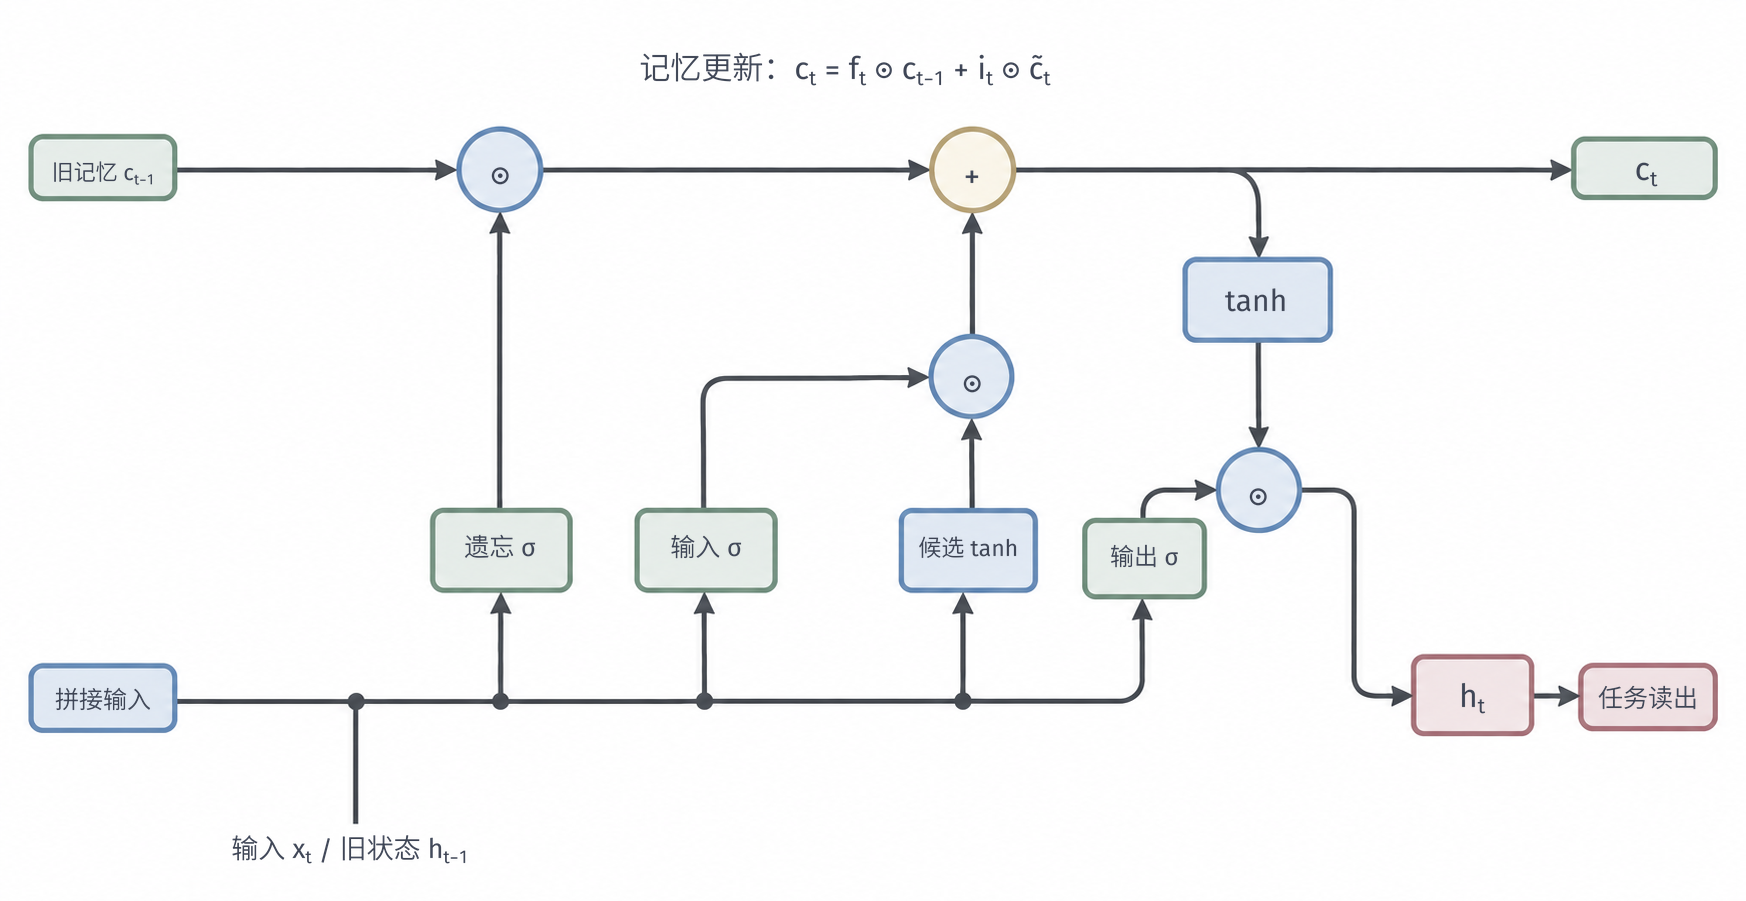
\includegraphics[width=147.828mm]{figures/03-models/02-neural-network-models/generated/rnn-lstm-cell/figure.png}
  \caption{LSTM更新与任务读出。框外左侧为当前输入$\bm x_t$和旧状态$\bm h^{(t-1)},\bm c^{(t-1)}$，右侧为新状态和预测$\widehat{\bm y}_t=g(\bm V\bm h^{(t)}+\bm c)$。三个Sigmoid模块分别产生遗忘门、输入门和输出门，Tanh框产生候选记忆；圆形$\odot$与$+$分别表示逐元素乘法和相加。门值0阻断对应路径的信息，门值1让信息通过。}
  \label{fig:rnn-lstm-cell}
\end{figure*}

如果暂把门与候选值看作已给定量，记忆路径对旧记忆的直接导数为$\operatorname{diag}(\bm{f}^{(t)})$。沿这条路径从$s$到$t$有
\begin{equation}
  \left.\frac{\partial\bm c^{(t)}}{\partial\bm c^{(s)}}\right|_{\mathrm{direct}}
    =\operatorname{diag}\!\left(\prod_{u=s+1}^{t}\bm f^{(u)}\right)\text{，}
  \label{eq:rnn-lstm-direct-memory}
\end{equation}
乘积按坐标进行。与普通RNN的$\bm D\bm W$相比，这条路径用可学习的保留率替代反复稠密混合；需要保存的坐标可令遗忘门接近1，并用较小输入门减少覆盖。这改变了式\eqref{eq:rnn-path-length-rate}中的逐步增益，通常没有缩短传播步数。但完整状态的Jacobian矩阵还包含$\bm h^{(t-1)}$影响各门和候选记忆的其他路径，直接路径与这些间接路径共同构成总导数。

\begin{example}[门值决定保留和写入]
  \label{ex:rnn-lstm-retention}
  考察一个记忆坐标，假设旧值为$2$，本步遗忘门为$0.9$、输入门为$0.2$、候选值为$0.5$。沿图~\ref{fig:rnn-lstm-cell}读取，左上$\odot$保留$0.9\times2=1.8$，中间$\odot$写入$0.2\times0.5=0.1$，再由上方$+$得到新记忆$1.9$。若输出门为$0.5$，右侧$\odot$产生隐藏输出$0.5\tanh(1.9)\approx0.478$，而非直接输出记忆值$1.9$。

  若之后100步不写入且遗忘门都为$0.99$，这份记忆沿直接路径的保留比例为$0.99^{100}\approx0.366$；门值为$0.9$时仅约$2.66\times10^{-5}$。加性记忆提供了可选择的保留率；小于1的门沿直接路径连续相乘，仍产生与距离有关的衰减。
\end{example}

图~\ref{fig:rnn-lstm-numerical-step}把例~\ref{ex:rnn-lstm-retention}扩展到两个记忆坐标。第一通道取较大的遗忘门和较小的输入门，主要保留旧值；第二通道反过来，主要写入候选值。$\odot$只在相同坐标之间相乘，不会把第一通道的门值作用到第二通道。两个通道可以采用不同的保留和写入比例。
\begin{figure*}[htbp]
  \centering
  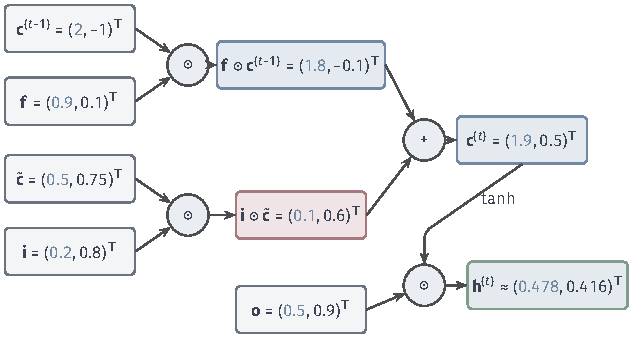
\includegraphics[width=107.107mm]{figures/03-models/02-neural-network-models/tikz/rnn-lstm-numerical-step/figure.pdf}
  \caption{二维LSTM的一步数值走查。蓝色与深灰数字分别表示两个通道；保留分支计算$\bm f\odot\bm c^{(t-1)}$，写入分支计算$\bm i\odot\widetilde{\bm c}$，二者相加得到新记忆，再经$\bm o\odot\tanh(\bm c^{(t)})$得到隐藏状态。所有数值均由图内向量逐坐标计算，第二通道结果为$0.9\tanh(0.5)\approx0.416$。图中暂把门值和候选值视为已知，不展开它们的仿射计算。}
  \label{fig:rnn-lstm-numerical-step}
\end{figure*}

记忆保持与信息读出仍要同时满足。即使直接路径没有明显衰减，过多写入也会覆盖证据；输出门较小或$\tanh(\bm c)$饱和时，任务损失仍可能难以作用于这段记忆。LSTM提供按任务选择保留、写入和读出的机制，完整梯度与预测表现需要对整个状态和读出分析。

训练仍使用BPTT，只需对记忆和隐藏两组状态共同求导。仅计上述单元，参数量为$4m(d+m+1)$，每步稠密仿射计算为$O(m(d+m))$，常数来自四组变换。增大初始遗忘门偏置可使初始保留比例较高，但门饱和也会减小自身的导数；这一选择需与长度和输入尺度匹配。

变体通常改变某条信息通路。\term{窥孔连接}（peephole connections）让门额外读取记忆坐标；耦合输入门与遗忘门可令$\bm{i}^{(t)}=\bm{1}-\bm{f}^{(t)}$，减少一组自由门。这些变体改变了门的依赖或自由度，适合程度需要在具体任务上比较\scite{greff2017}

% 避免两条完整变体引文在页底连续堆叠。
\Needspace{10\baselineskip}
若希望保留较宽记忆而减少循环映射成本，投影LSTM把记忆输出映射到更小的循环隐藏空间，使记忆宽度和循环宽度分开。投影把循环映射改为较小宽度，参数计数与前述等宽单元相应不同\scite{sak2014projection}

\subsection{GRU}
\label{sec:rnn-gru}

若希望简化状态管理，可以把记忆与隐藏输出合为一组变量。\term{门控循环单元}（gated recurrent unit, GRU）用更新门决定旧状态与候选状态的混合比例，用重置门控制候选计算怎样读取旧状态。这里采用Cho等原始形式的记号：更新门值越大，旧状态保留越多\scite{cho2014}

对同宽状态，方程为
\begin{equation}
  \begin{aligned}
    \bm{z}^{(t)}&=\operatorname{sigmoid}\!\left(
      \bm{U}_{\mathrm{z}}\bm{x}_t+\bm{W}_{\mathrm{z}}\bm{h}^{(t-1)}
      +\bm{b}_{\mathrm{z}}\right),\\
    \bm{r}^{(t)}&=\operatorname{sigmoid}\!\left(
      \bm{U}_{\mathrm{r}}\bm{x}_t+\bm{W}_{\mathrm{r}}\bm{h}^{(t-1)}
      +\bm{b}_{\mathrm{r}}\right),\\
    \widetilde{\bm{h}}^{(t)}&=\tanh\!\left(
      \bm{U}_{\mathrm{h}}\bm{x}_t
      +\bm{W}_{\mathrm{h}}(\bm{r}^{(t)}\odot\bm{h}^{(t-1)})
      +\bm{b}_{\mathrm{h}}\right),\\
    \bm{h}^{(t)}&=\bm{z}^{(t)}\odot\bm{h}^{(t-1)}
      +(\bm{1}-\bm{z}^{(t)})\odot\widetilde{\bm{h}}^{(t)}\text{。}
  \end{aligned}
  \label{eq:rnn-gru-update}
\end{equation}
每组$\bm{U}$、$\bm{W}$和偏置的形状与普通RNN相同。重置门接近零时，候选计算弱化旧状态；更新门接近1时，即使候选发生变化，输出也主要保留旧值。重置门调节候选读入的旧状态，更新门调节候选写入的比例，两者作用于不同计算位置。

图~\ref{fig:rnn-gru-cell}显示了候选分支和保留分支。单独看保留分支，其直接传播系数为$\bm{z}^{(t)}$；完整导数还包含门和候选的变化，与LSTM一样，直接分支之外的依赖也参与求导。

\begin{figure*}[htb]
  \centering
  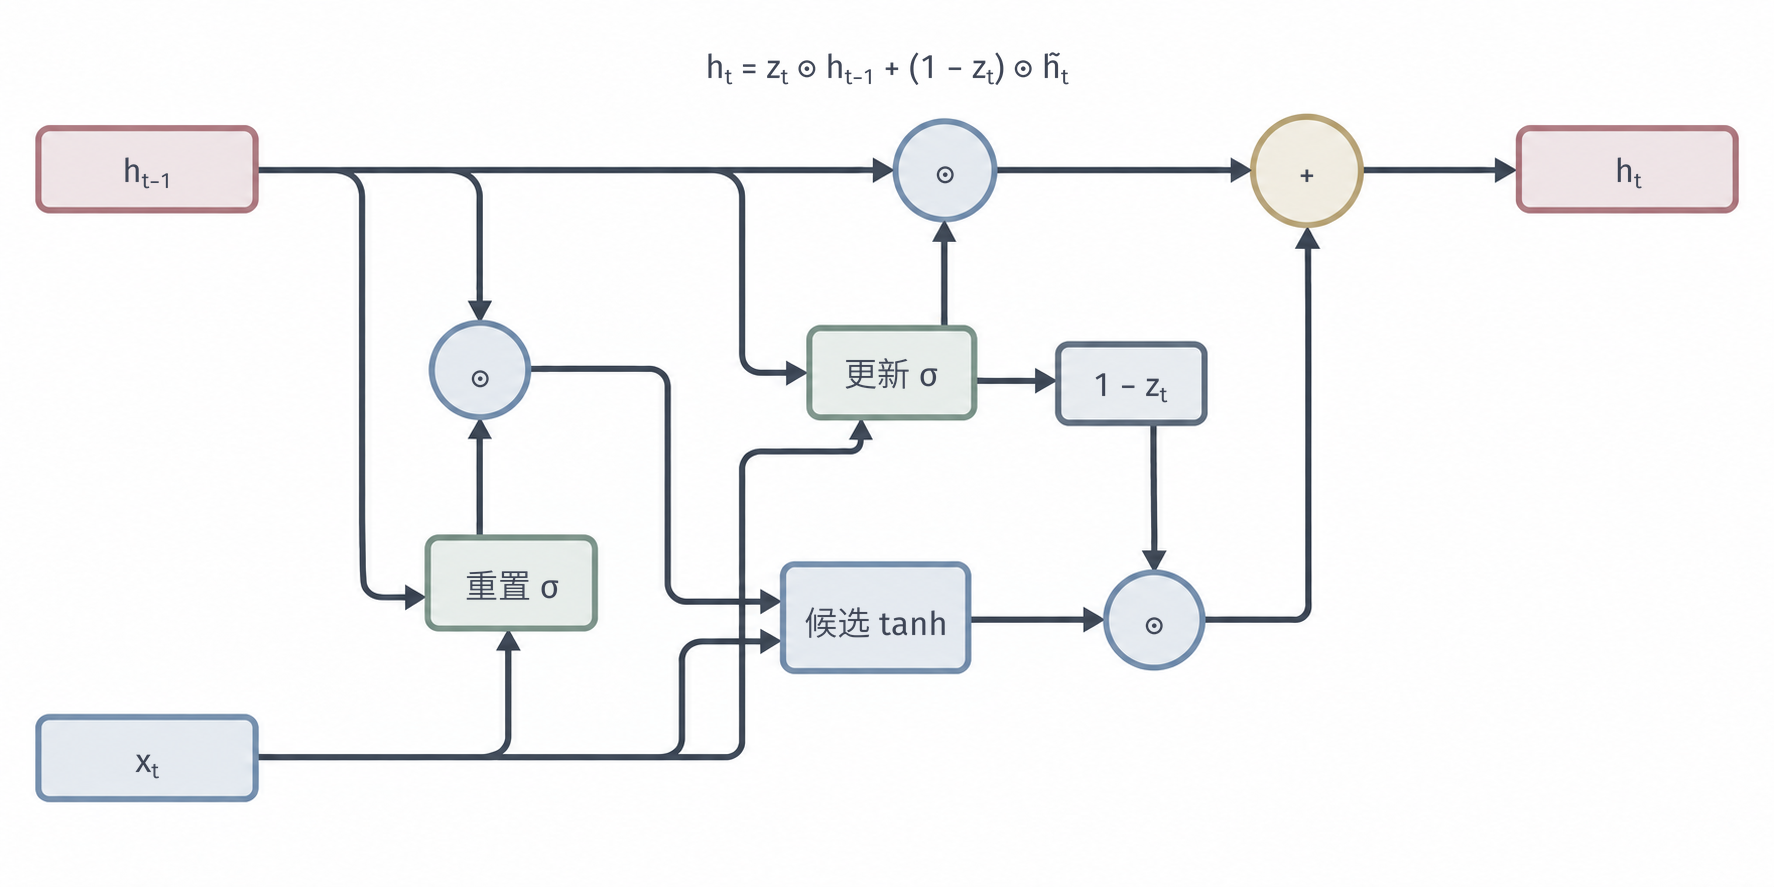
\includegraphics[width=150.199mm]{figures/03-models/02-neural-network-models/generated/rnn-gru-cell/figure.png}
  \caption{GRU的状态更新。左侧输入为$\bm x_t$和旧状态$\bm h^{(t-1)}$，右侧输出为新状态。组合输入将当前输入与旧状态一并送入门和候选模块。重置门参与候选计算；顶部两个$\odot$框则显式形成$\bm z^{(t)}\odot\bm h^{(t-1)}$与$(\bm1-\bm z^{(t)})\odot\widetilde{\bm h}^{(t)}$，再相加得到新状态。任务预测还需在新状态之后另接读出。}
  \label{fig:rnn-gru-cell}
\end{figure*}

GRU的长期保留对应更新门调节的直达分支。在需要延续记忆的坐标上，$\bm z^{(t)}$接近1时，状态更新接近复制旧值，沿保留路径的系数为各步$\bm z$的逐坐标乘积。候选分支的权重$\bm1-\bm z$同时较小，减少无关新输入覆盖已有状态。更新门接近0时则更多采用候选，允许网络改变当前记忆内容。

重置门的作用发生在候选计算中：它调节形成新候选时读取的旧状态量。重置门接近0、更新门接近1时，网络仍可以保留旧状态；更新门接近0时，即使重置门较大，旧信息也要通过非线性候选重新表达。没有独立记忆状态与输出门，还使GRU的保留内容和当前对外表示耦合得更紧。门接近恒等复制能改善一条梯度路径，门饱和、候选混合及读出仍可能限制长期学习。

在只用一组偏置的上述形式中，GRU单元参数量为$3m(d+m+1)$，少于等宽LSTM的四组变换，也只维护一个$m$维状态。代价是没有独立的记忆状态和输出门，存储与对外表示更直接地耦合。三组变换减少了等宽时的参数和状态存储，任务效果还取决于这种状态耦合是否适合目标；比较可在相近预算与预测条件下进行。

文献与软件还存在不同约定：有的把更新门定义为新候选的写入比例，有的把重置门放在$\bm{W}_{\mathrm{h}}\bm{h}^{(t-1)}$之后。前一种可通过交换$\bm{z}$与$1-\bm{z}$对应，后一种一般不能交换矩阵乘法与逐元素乘法，因此并非完全相同的更新。方程、偏置组数和门顺序共同确定具体GRU的计算与参数计数。

\section{基于注意力的循环神经网络}
\label{sec:rnn-attention}

在式\eqref{eq:rnn-encoder-decoder}中，全部输入只能经由同一个上下文向量被解码器读取。输入越长，需要同时保存和区分的细节可能越多；即使编码器使用LSTM，固定向量读出仍然要求不同生成步从同一压缩结果中恢复各自所需的信息。可以保留每个输入位置的编码状态，让解码器在生成每个符号时重新选择读取位置。

\subsection{注意力机制}
\label{sec:rnn-attention-mechanism}

\term{注意力机制}（attention mechanism）根据当前计算需求给一组表示分配权重，再加权聚合：解码器需要的信息改变时，读取的上下文也随之改变。令编码器状态为$\bm{h}_1,\ldots,\bm{h}_T\in\mathbb{R}^{m}$，这里下标表示被保存的位置，$\bm{h}_t=\bm{h}^{(t)}$。对第$j$个解码步，给定查询$\bm{q}^{(j)}\in\mathbb{R}^{r}$，计算
\begin{equation}
  \begin{aligned}
    e_{j,t}&=a(\bm{q}^{(j)},\bm{h}_t),\\
    \alpha_{j,t}&=\frac{\exp(e_{j,t})}
       {\sum_{u=1}^{T}\exp(e_{j,u})},\\
    \bm{c}^{(j)}&=\sum_{t=1}^{T}\alpha_{j,t}\bm{h}_t\text{。}
  \end{aligned}
  \label{eq:rnn-attention}
\end{equation}
评分函数$a$比较查询与候选表示的相关程度。Softmax使权重非负且总和为1，$\bm{c}^{(j)}$是本步的动态上下文。归一化只在有效输入位置上进行，填充位置通过掩码排除。对很大的得分减去最大值再取指数，不改变权重，却可避免指数溢出。

评分可以通过非线性组合学习，也可以使用内积。\term{加性注意力}（additive attention）先把查询和编码状态投影到同一评分空间，再给出标量：
\begin{equation}
  e_{j,t}=\bm{v}_{\mathrm{a}}^{\top}\tanh\!\left(
     \bm{W}_{\mathrm{q}}\bm{q}^{(j)}
     +\bm{W}_{\mathrm{h}}\bm{h}_t+\bm{b}_{\mathrm{a}}\right)\text{。}
  \label{eq:rnn-additive-attention}
\end{equation}
设评分空间宽度为$a$，则$\bm{W}_{\mathrm{q}}\in\mathbb{R}^{a\times r}$、$\bm{W}_{\mathrm{h}}\in\mathbb{R}^{a\times m}$、$\bm{v}_{\mathrm{a}},\bm{b}_{\mathrm{a}}\in\mathbb{R}^{a}$。它允许查询和编码状态原本具有不同维度。

\term{点积注意力}（dot-product attention）直接用内积评分，在$r=m$时可取$e_{j,t}=\langle\bm{q}^{(j)},\bm{h}_t\rangle$；一般形式可取$e_{j,t}=(\bm{q}^{(j)})^{\top}\bm{W}_{\mathrm{a}}\bm{h}_t$，其中$\bm{W}_{\mathrm{a}}\in\mathbb{R}^{r\times m}$。点积形式便于批量矩阵计算，加性形式通过额外非线性改变评分函数，两者的适合程度仍由任务和宽度决定。Transformer章会继续讨论缩放、多头和位置编码，这里只需理解评分、归一化和聚合。

\begin{example}[权重与上下文]
  \label{ex:rnn-attention-context}
  假设本步对三个位置的得分为$0,\log2,0$，相应状态为$(1,0)^{\top}$、$(0,2)^{\top}$、$(1,1)^{\top}$。归一化权重为$(1/4,1/2,1/4)$，上下文为$(1/2,5/4)^{\top}$。第二个位置贡献较大，但上下文仍混合了三个状态；软聚合把多个状态的贡献相加，最终预测还取决于这些状态的内容及后续计算。
\end{example}

\subsection{网络结构}
\label{sec:rnn-attentive-architecture}

动态上下文可以参与解码状态更新，也可以在更新后参与输出。Bahdanau等的模型用此前解码状态查询编码表示，先形成$\bm{c}^{(j)}$，再计算本步状态：
\begin{equation}
  \begin{aligned}
    \bm{q}^{(j)}&=\bm{s}^{(j-1)},\\
    \bm{s}^{(j)}&=F_{\mathrm{dec}}\!\left(
      \bm{s}^{(j-1)},\bm{e}(y_{j-1}),\bm{c}^{(j)}\right),\\
    \bm{p}^{(j)}&=G\!\left(\bm{s}^{(j)},\bm{c}^{(j)},\bm{e}(y_{j-1})\right)\text{。}
  \end{aligned}
  \label{eq:rnn-bahdanau-order}
\end{equation}
$G$是输出概率映射，包含所需的可学习变换和归一化。编码器可以双向读取输入，使每个位置的表示同时包含前后上下文；编码器读取完整源输入，解码器生成时仍只使用此前目标\scite{bahdanau2015}

Luong等则先计算本步解码状态，再用该状态查询，形成融合后的输出表示：
\begin{equation}
  \begin{aligned}
    \bm{s}^{(j)}&=F_{\mathrm{dec}}\!\left(
      \bm{s}^{(j-1)},\bm{e}(y_{j-1})\right),\\
    \bm{q}^{(j)}&=\bm{s}^{(j)},\qquad
    \widetilde{\bm{s}}^{(j)}=
       \tanh\!\left(\bm{W}_{\mathrm{c}}[\bm{s}^{(j)};\bm{c}^{(j)}]\right),\\
    \bm{p}^{(j)}&=\operatorname{softmax}\!\left(
      \bm{V}_{\mathrm{a}}\widetilde{\bm{s}}^{(j)}+\bm{b}_{\mathrm{a}}\right)\text{。}
  \end{aligned}
  \label{eq:rnn-luong-order}
\end{equation}
其输入馈送变体还把前一步融合表示送入下一步解码。两个模型的关键区别之一是查询产生的时机和上下文进入的路径，若把当前状态查询放进式\eqref{eq:rnn-bahdanau-order}而保留其余依赖，查询与本步更新就互相等待；具体架构通过明确先后次序建立可执行的计算\scite{luong2015}

\term{全局注意力}（global attention）对全部有效输入位置评分，生成$S$个符号通常需要$ST$个位置对评分。\term{局部注意力}（local attention）只考虑某个位置附近的窗口，可固定窗口推进方式，也可由状态预测中心。窗口降低了读取范围与评分数量，但可能遗漏远处证据；可学习中心、连续位置权重和边界处理还需明确。局部方法预先限制本步评分的候选位置；全局权重集中则仍在完整位置集合上评分。

图~\ref{fig:rnn-attention-paths}采用先查询、后更新的组织方式。保存的编码状态建立了一条从输出直接读取早期位置的路径，减轻了所有细节只能经过编码末状态的限制。它同时需要保存整段编码表示，每个生成步还要执行读取，代价与固定状态读出不同。

\begin{figure*}[htb]
  \centering
  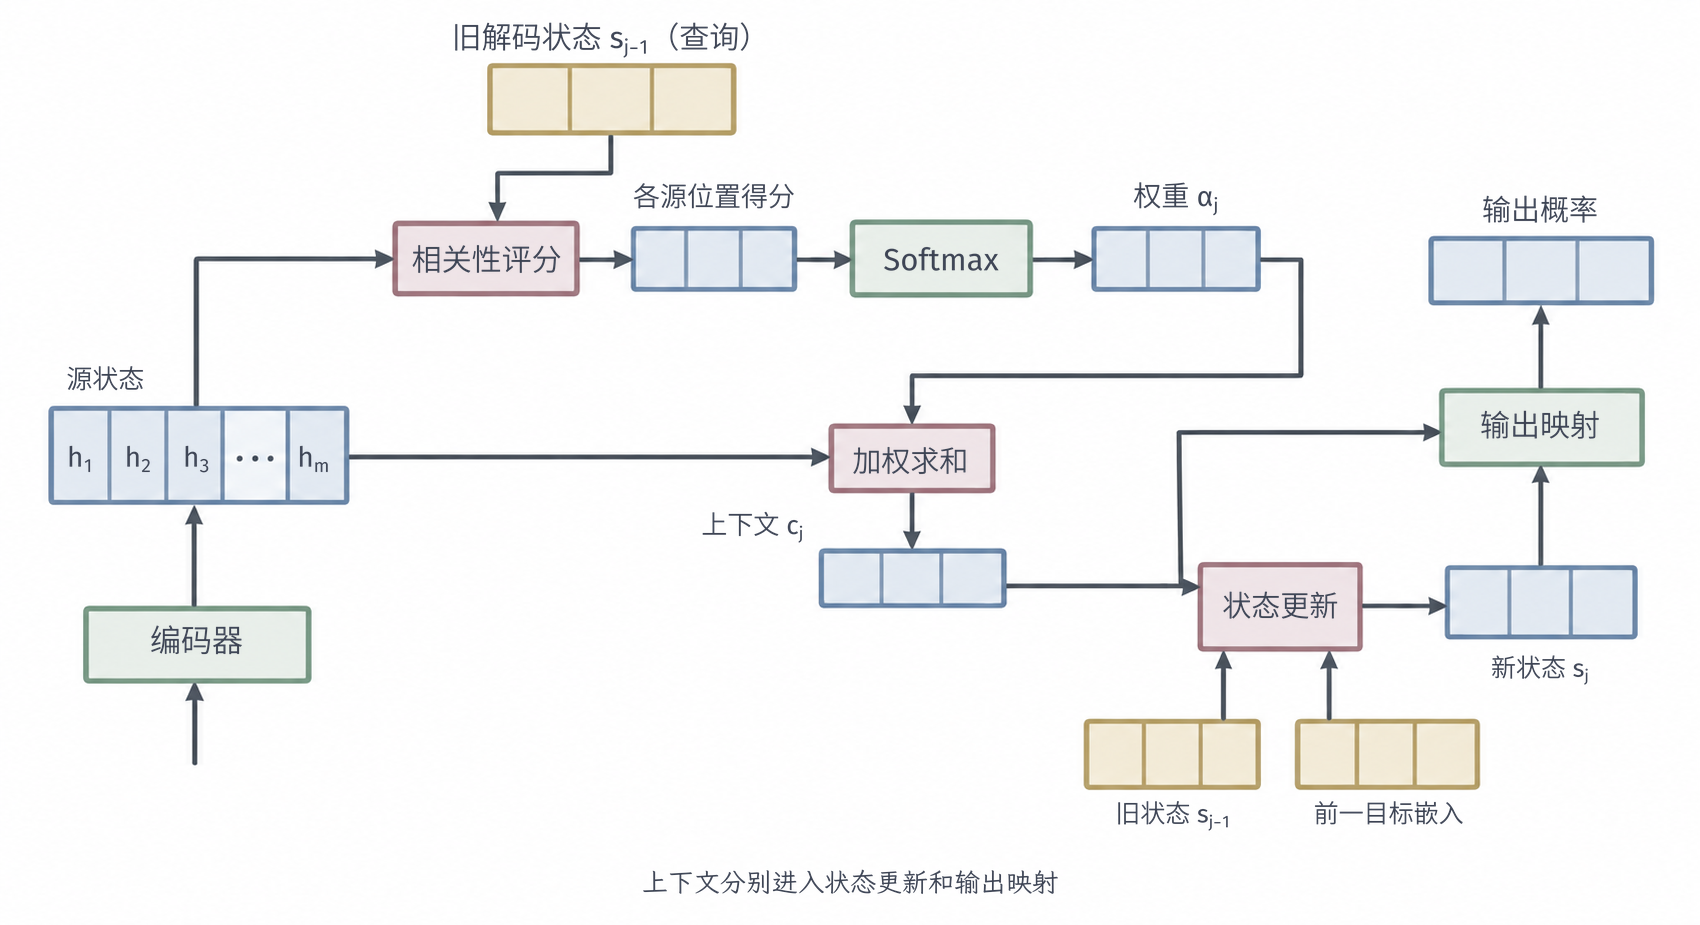
\includegraphics[width=143.933mm]{figures/03-models/02-neural-network-models/generated/rnn-attention-paths/figure.png}
  \caption{带注意力的一个解码步。左侧为保存的编码状态$\bm h_{1:T}$、旧解码状态和此前目标的嵌入，右侧为新解码状态和输出概率。查询先用旧解码状态产生权重$\bm\alpha_j=(\alpha_{j,1},\ldots,\alpha_{j,T})$，上下文再进入更新与输出映射；输出映射还可读取目标嵌入。编码状态在各解码步重复读取，图中不重新执行编码器。}
  \label{fig:rnn-attention-paths}
\end{figure*}


注意力对长期依赖的作用，可以从读取路径直接看出。暂固定本步评分和权重时，动态上下文对第$t$个编码状态的直接导数为
\begin{equation}
  \left.\frac{\partial\bm c^{(j)}}{\partial\bm h_t}\right|_{\bm\alpha_j\ \mathrm{fixed}}
       =\alpha_{j,t}\bm I\text{。}
  \label{eq:rnn-attention-direct-path}
\end{equation}
该分支从上下文直接到保存的表示，不再要求第$t$个状态经过其后全部编码状态才能被读取。权重若均匀，系数为$1/T$；若本步评分集中于相关位置，相应系数可以更大。这与普通时间链上的指数连乘具有不同的路径结构。

动态读取的对象是编码器已经形成的$\bm h_t$，其中保留了哪些历史仍由编码计算决定；评分过度分散或集中到无关位置时，相关证据的聚合贡献会减弱。保存各位置状态扩大了可访问范围，代价是随源长度增长的存储和读取。完整导数还包含评分随编码状态变化的分支，下一小节会把它与编码器、解码器的时间梯度合在一起。

\subsection{参数学习}
\label{sec:rnn-attention-learning}

编码器、评分函数、解码器和输出层可以按式\eqref{eq:rnn-sequence-likelihood}联合学习。软聚合可微，无需为每个目标另给一个位置标签。要理解注意力如何收到监督，暂固定查询并只看一个上下文节点。令$\bm{g}_{\mathrm{c}}^{(j)}=\partial L/\partial\bm{c}^{(j)}$，Softmax导数给出
\begin{equation}
  \frac{\partial L}{\partial e_{j,t}}
    =\alpha_{j,t}\left\langle
      \bm{g}_{\mathrm{c}}^{(j)},\bm{h}_t-\bm{c}^{(j)}\right\rangle\text{。}
  \label{eq:rnn-attention-score-gradient}
\end{equation}
其来源是$\partial\alpha_{j,u}/\partial e_{j,t}=\alpha_{j,u}(\mathbf{1}_{\{u=t\}}-\alpha_{j,t})$。增加某个得分会提高对应状态的相对权重，并降低其他权重；所以梯度比较的是该状态与当前平均上下文的差异，而不是仅看该状态的绝对值。

对编码状态还存在直接聚合贡献$\alpha_{j,t}\bm{g}_{\mathrm{c}}^{(j)}$，以及该状态改变评分产生的间接贡献。多个解码步的贡献相加后，再沿编码器的时间依赖回传；查询和解码状态也收到评分路径与输出路径的梯度。注意力缩短了部分信息与梯度路径，但编码器和解码器仍有循环依赖，权重过度集中或趋于零也可能削弱某些位置的监督。

\section{状态空间模型}
\label{sec:rnn-state-space}

门控调节保存，注意力调节读取；若还要改变时间依赖的执行方式，可以从状态转移的代数形式入手：让每一步更新能被高效组合，再在状态模块外加入投影、非线性与跨层连接。这里的\term{状态空间模型}（state space model, SSM）指用于神经序列网络的状态更新与读出模块；这个名称在控制和概率建模中还有更广含义，本节不讨论随机状态估计的完整框架。

\subsection{状态空间表示与并行计算基础}
\label{sec:rnn-ssm-foundations}

线性状态更新分别映射旧状态与当前输入后相加，输出再读取新状态及当前输入。网络可以学习这些映射的矩阵参数，将系统的动态响应用于序列预测；相关历史响应和离散计算见\BookSectionRef{sec:signal-analysis-state-history-kernels}{第一卷“数学准备”的线性状态历史响应小节}
与\BookSectionRef{sec:dynamical-discretization-scan}{第一卷“数学准备”的离散化与有序扫描节}。对连续输入$\bm{x}(\tau)\in\mathbb{R}^{d}$，表示为
\begin{equation}
  \frac{\mathrm{d}\bm{h}(\tau)}{\mathrm{d}\tau}
    =\bm{A}\bm{h}(\tau)+\bm{B}\bm{x}(\tau),
  \qquad
  \bm{y}(\tau)=\bm{C}\bm{h}(\tau)+\bm{D}\bm{x}(\tau)\text{。}
  \label{eq:rnn-continuous-ssm}
\end{equation}
其中$\bm{h}(\tau)\in\mathbb{R}^{m}$，$\bm{A}\in\mathbb{R}^{m\times m}$、$\bm{B}\in\mathbb{R}^{m\times d}$、$\bm{C}\in\mathbb{R}^{q\times m}$、$\bm{D}\in\mathbb{R}^{q\times d}$；$\bm{D}$给出当前输入直达输出的通路。$\tau$表示连续时间，避免与离散步数$t$混淆。此处先固定矩阵和步长，称为\term{线性时不变}（linear time-invariant, LTI）：叠加成立，转移规则也不随时间位置改变。

如果每个采样区间长$\Delta>0$且输入在区间内保持常值，解线性微分方程得到\term{零阶保持离散化}（zero-order hold discretization）：
\begin{equation}
  \begin{aligned}
    \overline{\bm{A}}&=\exp(\Delta\bm{A}),
    &\overline{\bm{B}}&=\int_0^{\Delta}\exp(u\bm{A})\bm{B}\,\mathrm{d}u,\\
    \bm{h}^{(t)}&=\overline{\bm{A}}\bm{h}^{(t-1)}
       +\overline{\bm{B}}\bm{x}_t,
    &\bm{y}_t&=\bm{C}\bm{h}^{(t)}+\bm{D}\bm{x}_t\text{。}
  \end{aligned}
  \label{eq:rnn-ssm-zoh}
\end{equation}
$\exp$是矩阵指数。$\bm{A}$可逆时，积分可写为$\bm{A}^{-1}(\exp(\Delta\bm{A})-\bm{I})\bm{B}$；积分形式在不可逆时仍有意义。网络也可以直接学习离散矩阵，不必总从连续方程出发。

在零初始状态、固定离散矩阵下，反复代入递推可得
\begin{equation}
  \begin{aligned}
    \bm{h}^{(t)}&=\sum_{u=1}^{t}
       \overline{\bm{A}}^{t-u}\overline{\bm{B}}\bm{x}_u,\\
    \bm{y}_t&=\sum_{k=0}^{t-1}\bm{K}_k\bm{x}_{t-k}
       +\bm{D}\bm{x}_t,\qquad
    \bm{K}_k=\bm{C}\overline{\bm{A}}^k\overline{\bm{B}}\text{。}
  \end{aligned}
  \label{eq:rnn-ssm-convolution}
\end{equation}
$\bm{K}_k\in\mathbb{R}^{q\times d}$是滞后$k$步的响应。它只依赖滞后而不依赖绝对位置，所以输出是一个因果卷积。非零初态还会增加$\bm{C}\overline{\bm{A}}^t\bm{h}^{(0)}$；时间变化或输入相关的系数一般不能并入同一个固定卷积核。

并行计算还有另一条基础。对已知的仿射更新$\bm{h}^{(t)}=\bm{A}_t\bm{h}^{(t-1)}+\bm{b}_t$，用二元组$(\bm{A}_t,\bm{b}_t)$表示一步变换。先执行$P$再执行$Q$的组合定义为
\begin{equation}
  (\bm{A}_Q,\bm{b}_Q)\circ(\bm{A}_P,\bm{b}_P)
   =(\bm{A}_Q\bm{A}_P,
      \bm{A}_Q\bm{b}_P+\bm{b}_Q)\text{。}
  \label{eq:rnn-affine-composition}
\end{equation}
这一有序复合使用卷一的\term{关联扫描}（associative scan）：
先组合连续片段，再恢复所有前缀。各步系数提前已知时，组合可先处理连续片段。依赖尚未算出旧状态的非线性更新，则需先获得相应状态才能确定下一变换。图~\ref{fig:rnn-scan}示意这一计算组织。

\begin{figure}[htb]
  \centering
  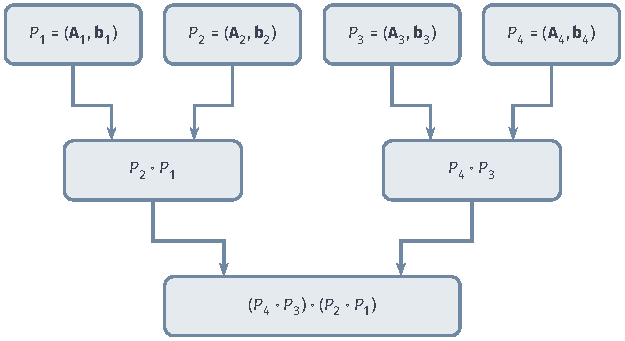
\includegraphics[width=105.791mm]{figures/03-models/02-neural-network-models/tikz/rnn-scan/figure.pdf}
  \caption{仿射状态更新的有序组合。四个单步变换先组成两个连续片段，再组成整段；$Q\circ P$表示先执行$P$再执行$Q$。平衡组合树展示的是扫描中的汇总阶段，完整前缀扫描还要把此前片段的结果传给各位置，才能得到每步状态。树形计算可缩短依赖深度，但不改变输入顺序。}
  \label{fig:rnn-scan}
\end{figure}

对逐坐标仿射更新，工作高效的扫描可用$O(Tm)$总运算量和$O(\log T)$组合深度得到前缀；稠密矩阵组合还要执行矩阵乘法，成本随状态宽度另行增加。普通RNN的非线性组合也通常无法保持固定大小、便于计算的仿射表示。可并行的条件是各步系数可提前取得、组合闭合且足够便宜；若系数必须由尚未计算的旧状态产生，就不能直接预先扫描。

\begin{example}[同一状态模型的递推与卷积]
  \label{ex:rnn-ssm-equivalence}
  取标量更新$h^{(t)}=\tfrac12 h^{(t-1)}+x_t$、$y_t=h^{(t)}$、$h^{(0)}=0$，输入为$(1,2,0)$。递推得到$(1,5/2,5/4)$。卷积核为$(1,1/2,1/4,\ldots)$，故第三步输出为$0+\tfrac12\times2+\tfrac14\times1=5/4$。整段训练可以按卷积组织，逐步预测可以按状态组织；相同输出来自相同模型的代数等价，而不是两套分别训练的参数。
\end{example}

\subsection{HiPPO}
\label{sec:rnn-hippo}

前述矩阵形式还没有回答状态应保存哪种历史。\term{高阶多项式投影}（high-order polynomial projection operators, HiPPO）把记忆写成一个明确的近似问题：用有限个多项式基函数的系数概括此前输入。相比只保存一个滑动平均，多个系数可以描述历史中的不同变化形态\scite{gu2020hippo}

\subsubsection{投影系数保存什么}
\label{sec:rnn-hippo-memory}

设标量历史信号为$f(u)$，在当前时刻$\tau$选定历史权重测度$\mu_\tau$和相应正交归一基$p_0(u;\tau),\ldots,p_{m-1}(u;\tau)$。在该测度下平方可积时，投影系数与近似信号为
\begin{equation}
  c_i(\tau)=\int f(u)p_i(u;\tau)\,\mathrm{d}\mu_\tau(u),
  \qquad
  \widehat f_\tau(u)=\sum_{i=0}^{m-1}c_i(\tau)p_i(u;\tau)\text{。}
  \label{eq:rnn-hippo-projection}
\end{equation}
它在所选$m$维基函数空间中最小化加权平方误差。状态记录这组基函数系数；每个系数汇集一个历史形状的影响，权重与有限基函数数目共同决定可保留的细节。

\subsubsection{在线更新与网络组织}
\label{sec:rnn-hippo-architecture}

例如缩放Legendre版本在$[0,\tau]$上采用均匀权重，将整个历史区间缩放到固定区间上的Legendre多项式。使用从零开始的$i,j\in\{0,\ldots,m-1\}$，其连续系数更新可写为
\begin{equation}
  \begin{aligned}
    \frac{\mathrm{d}\bm{c}(\tau)}{\mathrm{d}\tau}
      &=-\frac{1}{\tau}\bm{H}\bm{c}(\tau)
        +\frac{1}{\tau}\bm{b}f(\tau),\qquad \tau>0,\\
    H_{i,j}&=
      \begin{cases}
        \sqrt{(2i+1)(2j+1)},&i>j,\\
        i+1,&i=j,\\
        0,&i<j,
      \end{cases}
      \qquad b_i=\sqrt{2i+1}\text{。}
  \end{aligned}
  \label{eq:rnn-hippo-legs}
\end{equation}
随时间变化的$1/\tau$反映历史区间不断扩张，更新矩阵也随当前时间改变。$m=1$时，$c_0$是整个区间的均值，其导数为$(f(\tau)-c_0(\tau))/\tau$，这给出了系数更新的直观核验。离散实现需选择初始化和离散化，不能在$\tau=0$直接代入。

测度决定“哪些历史值得近似”：固定窗口强调近期区间，指数权重弱化久远输入，随时间扩张的均匀区间覆盖全部过去，但固定阶数的分辨率会受到区间增长影响。HiPPO提供状态构造原则和相应结构矩阵，完整预测网络仍需要输入变换、读出及学习目标。可以固定投影动态、学习前后变换，也可以以结构矩阵初始化后再调整；后者需要重新检查状态是否仍满足原来的投影含义。投影误差的性质不能直接代替任务泛化误差。


图~\ref{fig:rnn-hippo}展示了一种把投影记忆接入任务网络的方式。实际观测可先经过可学习映射形成$f(\tau)$；投影更新维护系数，任务读出利用系数产生预测。若输入有多个特征，可以为各通道分别维护一组系数，再混合通道。重构历史使用已选定的基函数，任务读出则由监督目标决定，两者用途不同。
\begin{figure}[htb]
  \centering
  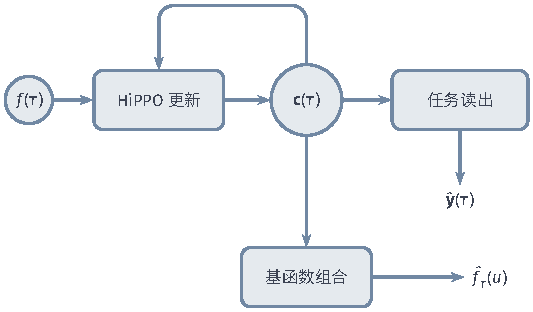
\includegraphics[width=90.293mm]{figures/03-models/02-neural-network-models/tikz/rnn-hippo/figure.pdf}
  \caption{HiPPO投影记忆与任务网络的一种组合。反馈维护系数状态，读出产生任务预测；下方将同一系数与基函数组合，近似重构历史信号。HiPPO本身规定记忆表示及更新，图中的任务读出与输入特征映射可另行学习，并非唯一的HiPPO网络架构。}
  \label{fig:rnn-hippo}
\end{figure}

若投影动态固定，任务损失训练输入映射和读出；输入映射可学习时，梯度仍需经过投影递推回到此前输入特征。若进一步训练投影矩阵，模型获得调整动态的自由，也放松了投影所规定的约束。固定投影动态维持了原来的投影约束，训练矩阵则让任务调整状态响应；参数范围决定当前模型保留哪种投影含义。

\subsubsection{历史覆盖与长期依赖的边界}
\label{sec:rnn-hippo-long-memory}

LegS把全部过去放进随时间扩张的区间，没有用一个固定窗口把早期输入直接删除。最低阶系数是均值：在$[0,\tau]$上，$c_0(\tau)=\tau^{-1}\int_0^\tau f(u)\,\mathrm du$。时刻$u$附近面积为$\varepsilon$的窄脉冲，对这个均值的贡献约为$\varepsilon/\tau$，随当前时刻按倒数减弱，而不是按已经经过的更新步数以固定比例反复衰减。

这个性质也可从状态更新看出。对$0<\sigma<\tau$，将$[\sigma,\tau]$间的输入固定，初始系数扰动满足
\begin{equation}
  \delta\bm c(\tau)
    =\exp\!\left[-\bm H\log(\tau/\sigma)\right]\delta\bm c(\sigma)\text{。}
  \label{eq:rnn-hippo-time-ratio}
\end{equation}
因为此区间的齐次更新是$\delta\dot{\bm c}=-\bm H\delta\bm c/\tau$，积分变量是$\log\tau$。与固定矩阵的$\exp(\bm A(\tau-\sigma))$相比，LegS按时间比值组织保留；最低阶模式的系数为$\sigma/\tau$。完整状态传播还包含其他模式及范数常数，任务梯度另经过输入映射和读出；最低阶模式只展示了时间比值的一个保留尺度。

多个系数提供的不是多个历史位置，而是多个形状特征。取$p_0=1$、$p_1=\sqrt3(2u/\tau-1)$，对线性历史$f(u)=a+bu$，两个系数为
\begin{equation}
  c_0=a+\frac{b\tau}{2},\qquad c_1=\frac{b\tau}{2\sqrt3}\text{。}
  \label{eq:rnn-hippo-linear-example}
\end{equation}
代回基函数组合即可精确恢复这条线性函数：第一个系数保存水平，第二个补上趋势。若历史含有很多窄尖峰，两个系数便不足以定位每个尖峰；提高阶数增加分辨能力，也增加状态与计算成本。

因此，HiPPO把长期记忆转为有明确误差准则的在线压缩。它适合考察较长区间上的形状和趋势，固定阶数、有限精度、所选测度与信号变化共同限制可恢复细节。模型若需要精确取回任意久远符号，还需检验相应信息在投影后是否可区分；任务网络的非线性与读出同样可能带来额外学习困难。

\subsection{S4}
\label{sec:rnn-s4}

利用式\eqref{eq:rnn-ssm-convolution}并行训练，还需要高效产生长度为$T$的卷积核。稠密$m\times m$矩阵逐步计算$\overline{\bm{A}}^k\overline{\bm{B}}$需要重复矩阵向量乘法；直接对某些HiPPO矩阵进行普通对角化又可能数值不稳定。\term{结构化状态空间序列模型}（structured state space sequence model, S4）利用状态矩阵的特殊分解加快递推与核生成\scite{gu2022s4}

\subsubsection{结构矩阵与核生成}
\label{sec:rnn-s4-structure}

其关键结构之一是\term{对角加低秩}（diagonal plus low-rank, DPLR）：在合适的复数坐标系中写为
\begin{equation}
  \bm{A}=\bm{\Lambda}-\bm{P}\bm{Q}^{*}\text{，}
  \label{eq:rnn-s4-dplr}
\end{equation}
其中$\bm{\Lambda}\in\mathbb{C}^{m\times m}$是对角矩阵，$\bm{P},\bm{Q}\in\mathbb{C}^{m\times r}$，秩$r$较小，$*$表示共轭转置。这个坐标系来自正规矩阵加低秩结构的酉变换；正规矩阵$\bm{N}$满足$\bm{N}\bm{N}^{*}=\bm{N}^{*}\bm{N}$，其酉对角化避免任意病态基变换，加入低秩项后的$\bm{A}$则不必正规。输入和输出映射也随坐标一起变换，实际输出可通过共轭配对保持实数。

S4采用的双线性离散化为
\begin{equation}
  \begin{aligned}
    \overline{\bm{A}}&=
      (\bm{I}-\tfrac{\Delta}{2}\bm{A})^{-1}
      (\bm{I}+\tfrac{\Delta}{2}\bm{A}),\\
    \overline{\bm{B}}&=
      (\bm{I}-\tfrac{\Delta}{2}\bm{A})^{-1}\Delta\bm{B}\text{，}
  \end{aligned}
  \label{eq:rnn-s4-bilinear}
\end{equation}
需保证逆矩阵存在。DPLR形式使相关逆矩阵作用可以通过对角运算和低秩修正计算；固定秩时，一步递推可达到$O(m)$量级，而不是稠密状态转移的$O(m^2)$。

核生成也利用这套结构。把长度为$T$的核视为一个有限多项式，用几何和恒等式可写为
\begin{equation}
  \begin{aligned}
    \bm{G}_T(z)&=\sum_{k=0}^{T-1}\bm{K}_k z^k\\
      &=\bm{C}\left[\bm{I}-(z\overline{\bm{A}})^T\right]
         (\bm{I}-z\overline{\bm{A}})^{-1}\overline{\bm{B}}\text{，}
  \end{aligned}
  \label{eq:rnn-s4-generating-function}
\end{equation}
第二行适用于所写逆矩阵存在时，$T$表示有限核长度，矩阵上的$T$是幂次而非转置。要看清这个逆怎样利用DPLR结构，下面固定单输入单输出情形，记$\bm B=\bm b$、$\bm C=\bm c^*$，其中$\bm b,\bm c\in\mathbb C^m$；此时$\bm G_T$退化为标量多项式$G_T$，低秩$r$不随$m,T$增长。

由双线性离散化，
\[
  \bm I-z\overline{\bm A}
    =(\bm I-\tfrac{\Delta}{2}\bm A)^{-1}
      \left[(1-z)\bm I-\frac{\Delta}{2}(1+z)\bm A\right]\text{。}
\]
对$z\neq-1$，提出方括号中的系数，可将离散逆矩阵作用改写为
\begin{equation}
  \begin{aligned}
    \xi(z)&=\frac{2}{\Delta}\frac{1-z}{1+z},\\
    (\bm I-z\overline{\bm A})^{-1}\overline{\bm b}
      &=\frac{2}{1+z}(\xi(z)\bm I-\bm A)^{-1}\bm b\text{。}
  \end{aligned}
  \label{eq:rnn-s4-resolvent}
\end{equation}
其中$\overline{\bm b}=(\bm I-\Delta\bm A/2)^{-1}\Delta\bm b$。右侧的$(\xi\bm I-\bm A)^{-1}$称为预解矩阵（resolvent）。双线性变换把离散频率点$z$转为连续状态矩阵的频率变量$\xi$，上式仍以相关逆存在为前提。

核只保留有限长度，因此求值还带有截断因子。在$T$个单位根
$z_\ell=\exp(-2\pi\mathrm i\ell/T)$、$\ell=0,\ldots,T-1$上，$\mathrm i$为虚数单位，$z_\ell^T=1$，因此可以共用修正后的输出行
\begin{equation}
  \bm c_T^*=\bm c^*(\bm I-\overline{\bm A}^{T})\text{。}
  \label{eq:rnn-s4-finite-readout}
\end{equation}
代入式\eqref{eq:rnn-s4-generating-function}与式\eqref{eq:rnn-s4-resolvent}，对$z_\ell\neq-1$得到
\begin{equation}
  G_T(z_\ell)=\frac{2}{1+z_\ell}
    \bm c_T^*(\xi(z_\ell)\bm I-\bm A)^{-1}\bm b\text{。}
  \label{eq:rnn-s4-root-evaluation}
\end{equation}
这里利用$z^T=1$才把修正行统一为$\bm c_T^*$；一般$z$处仍须保留$\bm I-(z\overline{\bm A})^T$，修正项与$\bm I-\overline{\bm A}^T$在一般求值点上不同。

现在代入$\bm A=\bm\Lambda-\bm P\bm Q^*$。记$\lambda_j$为$\bm\Lambda$的第$j$个对角元素，并令
\[
  \bm R_\xi=(\xi\bm I-\bm\Lambda)^{-1}
    =\operatorname{diag}\!\left(
       \frac1{\xi-\lambda_1},\ldots,\frac1{\xi-\lambda_m}\right)\text{。}
\]
Woodbury恒等式把原来的$m\times m$逆化为对角逆和一个$r\times r$逆：
\begin{equation}
  (\xi\bm I-\bm A)^{-1}
    =\bm R_\xi-\bm R_\xi\bm P
       (\bm I_r+\bm Q^*\bm R_\xi\bm P)^{-1}
       \bm Q^*\bm R_\xi\text{。}
  \label{eq:rnn-s4-woodbury}
\end{equation}
将其代入式\eqref{eq:rnn-s4-root-evaluation}，只需计算
$\bm c_T^*\bm R_\xi\bm b$、$\bm c_T^*\bm R_\xi\bm P$、
$\bm Q^*\bm R_\xi\bm b$和$\bm Q^*\bm R_\xi\bm P$，再作小矩阵求逆与乘法。每个对象的元素都是如下形式的求和：
\begin{equation}
  \bm u^*\bm R_\xi\bm v
    =\sum_{j=1}^{m}\frac{\overline{u_j}v_j}{\xi-\lambda_j}\text{，}
  \label{eq:rnn-s4-cauchy-sum}
\end{equation}
其中$\bm u$取$\bm c_T$或$\bm Q$的列，$\bm v$取$\bm b$或$\bm P$的列，$\overline{u_j}$表示复共轭。求和中的倒数因子$1/(\xi(z_\ell)-\lambda_j)$就是\term{Cauchy核}（Cauchy kernel）。因此加速的对象是许多频率点共享谱参数的这组求和，而不是为每个频率重新求一个一般稠密逆矩阵。

上述分解要求$\xi\bm I-\bm\Lambda$及低秩修正中的逆存在。若某个采样点使中间表达式奇异，应回到有限多项式求值，或使用已消去可去奇点的等价形式。偶数$T$还会包含$z_{T/2}=-1$，此点的$\xi$表达式有奇点；由$\bm I+\overline{\bm A}=2(\bm I-\Delta\bm A/2)^{-1}$可单独得到
\[
  G_T(-1)=\frac{\Delta}{2}\bm c_T^*\bm b
  \qquad(T\text{为偶数})\text{。}
\]
取得全部$T$个单位根处的值后，逆DFT恢复长度为$T$的核系数，可用FFT实现。这里保留的是有限多项式的值，不是无限序列频率响应的直接采样。

固定秩下，逐点直接执行式\eqref{eq:rnn-s4-cauchy-sum}仍需$O(mT)$求和工作，形成$\bm c_T$也有成本；上述恒等式本身并未证明近线性核生成。原始S4在相应快速结构算法下给出关于$m+T$的近线性分析，具体算法与数值实现仍需另行核对。得到核后，LTI状态模块可用适当补零的FFT卷积处理整段序列，单通道卷积的成本为$O(T\log T)$，核生成还包含前述结构求值与修正读出的工作。逐步预测改用同一组离散参数递推，无需保存全部历史输入。

\subsubsection{完整层、训练与逐步预测}
\label{sec:rnn-s4-architecture}

一个标量SSM只完成一条序列上的线性变换。完整S4层可为$d$个输入通道各设一个$m$维状态模块，得到$\bm y_t\in\mathbb R^d$，再作非线性变换和逐位置通道混合，例如
\begin{equation}
  \bm u_t=\bm M\,\phi(\bm y_t)+\bm b_{\mathrm{mix}},
  \qquad\bm M\in\mathbb R^{d\times d}\text{。}
  \label{eq:rnn-s4-channel-layer}
\end{equation}
$\phi$逐坐标作用，$\bm u_t$是本层输出特征，可送入下一层或任务头。维度匹配时还可以加入跨层残差与归一化。时间模块传播各通道的历史，通道混合再使不同特征相互作用；多个这样的层构成非线性序列网络。

图~\ref{fig:rnn-s4}把同一层的两种计算方式并列。整段输入已经给定时，由结构参数生成因果卷积核，再对各通道计算卷积；逐步预测时，维护各通道状态并直接递推。外部非线性与通道映射相同，切换的是线性状态模块的计算形式。
\begin{figure*}[htb]
  \centering
  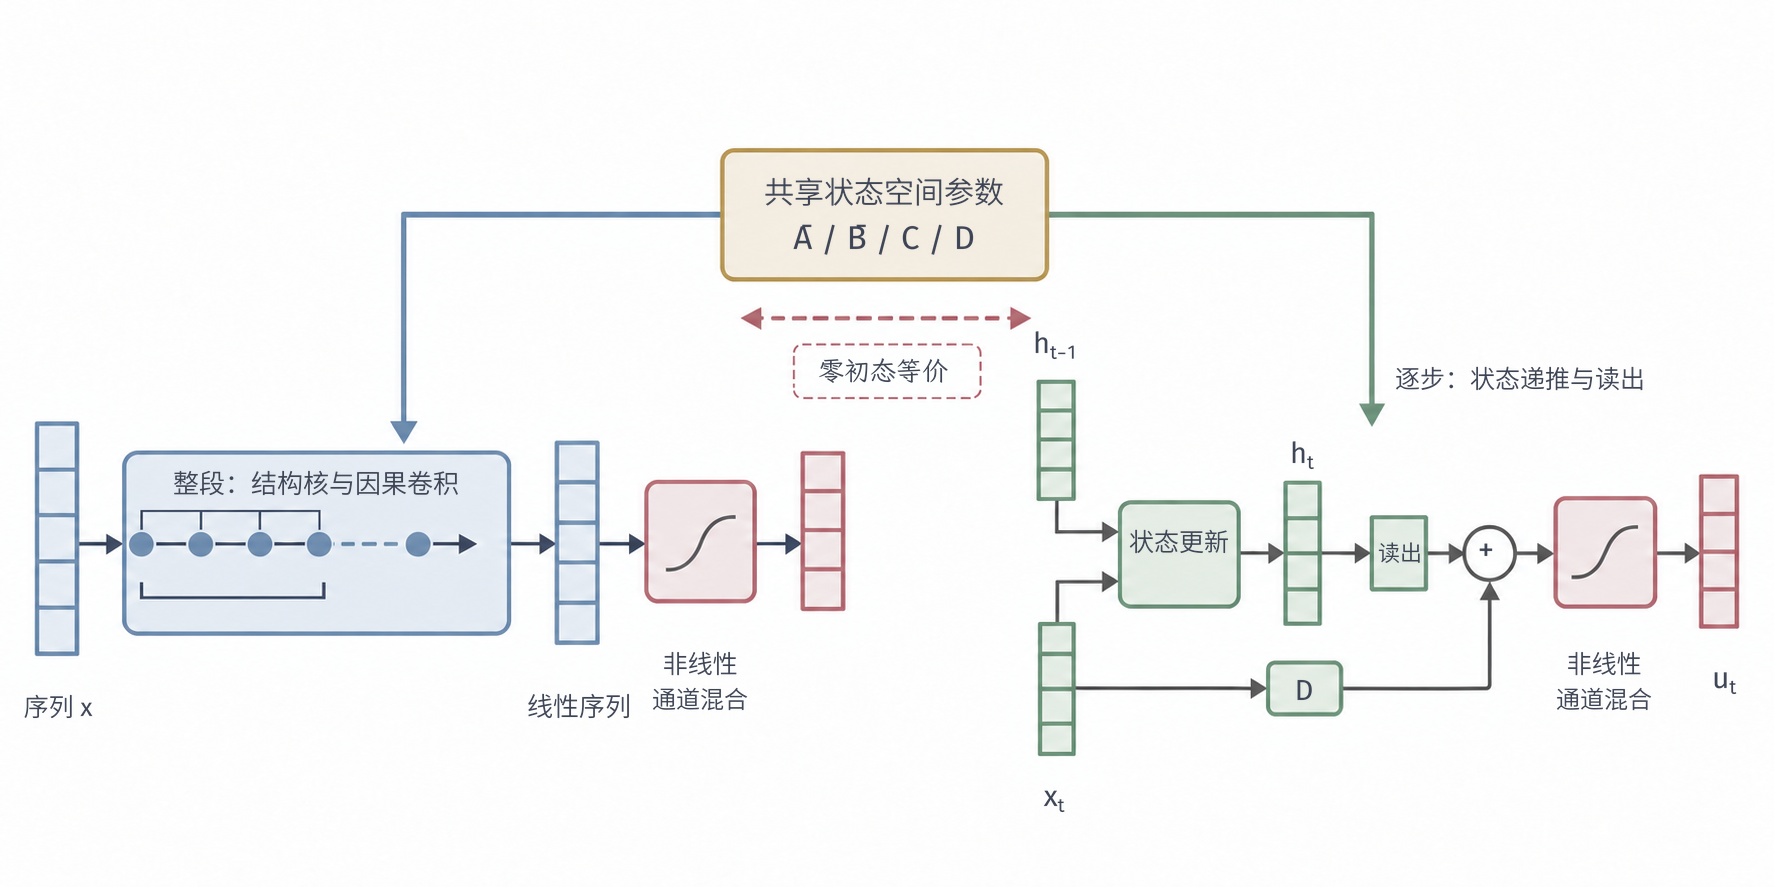
\includegraphics[width=150.199mm]{figures/03-models/02-neural-network-models/generated/rnn-s4/figure.png}
  \caption{S4层的整段与逐步计算。两个路径共享同一组离散状态参数及后续通道映射，上方路径提供共享参数，跨路径虚线说明零初态下的等价关系。整段分支把直达映射$\bm D$并入零滞后卷积系数，$\widetilde{\bm K}_0=\bm K_0+\bm D$，其余滞后系数不变。零初态时，因果卷积与递推得到相同线性序列输出；非零初态需要补上对应初态响应。图中$\bm u$是层输出特征，任务预测还需相应读出。}
  \label{fig:rnn-s4}
\end{figure*}

结构参数、输入输出映射、步长与通道映射由任务损失联合学习。卷积路径的反向计算对结构参数所生成的同一个核求导；预测切到递推时，需要使用与训练一致的离散化、因果约定和初始化。整个网络可以非线性，卷积等价只针对满足LTI条件的状态模块。

HiPPO-LegS的$1/\tau$更新与S4中的固定结构动态也应分清。S4借用结构矩阵和初始化思想，使网络可以学习有用的时间响应；当前模块的固定动态与LegS随历史区间扩展的更新有不同的时间含义。DPLR结构首先服务于高效计算，训练后的稳定性与长期响应还要检查参数取值。

\subsubsection{时间尺度与长期依赖}
\label{sec:rnn-s4-long-memory}

S4保存多久，与离散状态矩阵的模式有关。在可对角化情形下，$\bm K_k=\bm C\overline{\bm A}^k\overline{\bm B}$是多个指数模式的加权组合。某模式的特征值$\bar\lambda_j$满足$0<|\bar\lambda_j|<1$时，其幅度按$|\bar\lambda_j|^k$衰减，相应以步数计的时间尺度为
\begin{equation}
  \tau_{\mathrm{steps},j}=-\frac{1}{\log|\bar\lambda_j|}\text{。}
  \label{eq:rnn-s4-timescale}
\end{equation}
幅度经过这个步数约降到原来的$e^{-1}$。接近1的模式保留较久，较小的模式强调近期；复数模式还可表示振荡。不同时间尺度共同形成历史响应，输入映射决定往哪些模式写入，输出映射决定哪些模式参与预测。

对连续特征值$\lambda_j$，双线性离散化给出$\bar\lambda_j=(1+\Delta\lambda_j/2)/(1-\Delta\lambda_j/2)$。左半平面的特征值映入单位圆内，步长又改变离散时间尺度。特征值只描述模式，非正规矩阵的短期放大与数值条件仍需考虑；结构可高效计算，也不代表任意自由参数都稳定。

长期影响在输入输出层面写为$\partial\bm y_t/\partial\bm x_s=\bm K_{t-s}$，$s<t$；当前输入的导数还包含直接项$\bm D$。卷积路径直接计算这个历史响应，训练时不必按普通RNN的非线性单元逐步展开；但FFT与递推计算的是同一个映射，相关历史响应的导数也相同。若核在相关距离已经衰减，早期证据仍然弱；若读写映射没有利用慢模式，长时间尺度也不会自动转成任务所需的记忆。

S4因而同时改善状态的结构设计和整段计算。固定LTI模块对同一滞后使用同一响应，适合学习多尺度时间关系，却不能在单个模块中按每次输入的内容改写保留率。非线性堆叠扩展了网络表达，按内容选择状态的另一种做法则是下面的Mamba。

\subsection{Mamba}
\label{sec:rnn-mamba}

固定LTI更新对相同滞后使用相同响应。若输入流中只有某些符号需要保留，而它们出现的位置不固定，仅按滞后衰减便难以直接按内容筛选。\term{Mamba}采用选择性状态空间更新，让部分系数由当前输入产生，改变哪些内容写入、保留或读出。本节采用原始Mamba架构\scite{gu2023mamba}

\subsubsection{选择性状态更新}
\label{sec:rnn-mamba-selection}

为看清选择性，考察预处理后一个通道的标量输入$x_t$与$m$维状态。固定可学习的连续对角矩阵$\bm A$，由当前输入特征产生$\Delta_t>0$、$\bm B_t\in\mathbb R^m$和$\bm C_t\in\mathbb R^{1\times m}$，采用零阶保持时
\begin{equation}
  \begin{aligned}
    \overline{\bm A}_t&=\exp(\Delta_t\bm A),\\
    \overline{\bm B}_t&=\int_0^{\Delta_t}\exp(u\bm A)\bm B_t\,\mathrm du,\\
    \bm h^{(t)}&=\overline{\bm A}_t\bm h^{(t-1)}+\overline{\bm B}_t x_t,\\
    y_t&=\bm C_t\bm h^{(t)}+D x_t\text{。}
  \end{aligned}
  \label{eq:rnn-mamba-selection}
\end{equation}
$D$是通道的直接输入系数。输入相关不要求$\bm A$每步重新生成，选择性来自步长、写入和读出映射。多个通道各有状态，并由通道投影组合。

常用参数化令$A_{i,i}=-\exp(a_i)$、$\Delta_t=\operatorname{softplus}(d_t)$，其中$a_i$是参数，$d_t$由输入映射并加入偏置产生。这分别限制连续模式的衰减方向与步长的正值。$\bm B_t$决定输入写入哪些状态坐标，$\bm C_t$决定本步从哪些坐标形成输出。离散化是模型定义的一部分，复现时需核对写入项采用的具体规则。

取标量特例$A=-1$、$B_t=1$、$D=0$，更新成为
\begin{equation}
  h^{(t)}=e^{-\Delta_t}h^{(t-1)}+(1-e^{-\Delta_t})x_t\text{。}
  \label{eq:rnn-mamba-gate-special-case}
\end{equation}
小步长主要保留旧状态，大步长更多采用当前输入。这与控制门有明确联系，但完整模块具有多个状态坐标及输入相关的读写映射，其读写自由度由完整状态和各选择映射共同确定。

\subsubsection{完整模块的两条分支}
\label{sec:rnn-mamba-architecture}

选择性SSM只负责时间方向的状态计算。图~\ref{fig:rnn-mamba}把它放回完整模块：输入归一化与投影后分成两条支路，一条经过短因果卷积和SiLU，产生送入SSM的特征；另一条经过SiLU形成调制向量。SSM输出与调制向量逐坐标相乘，再经过输出投影和残差相加。
\begin{figure*}[htb]
  \centering
  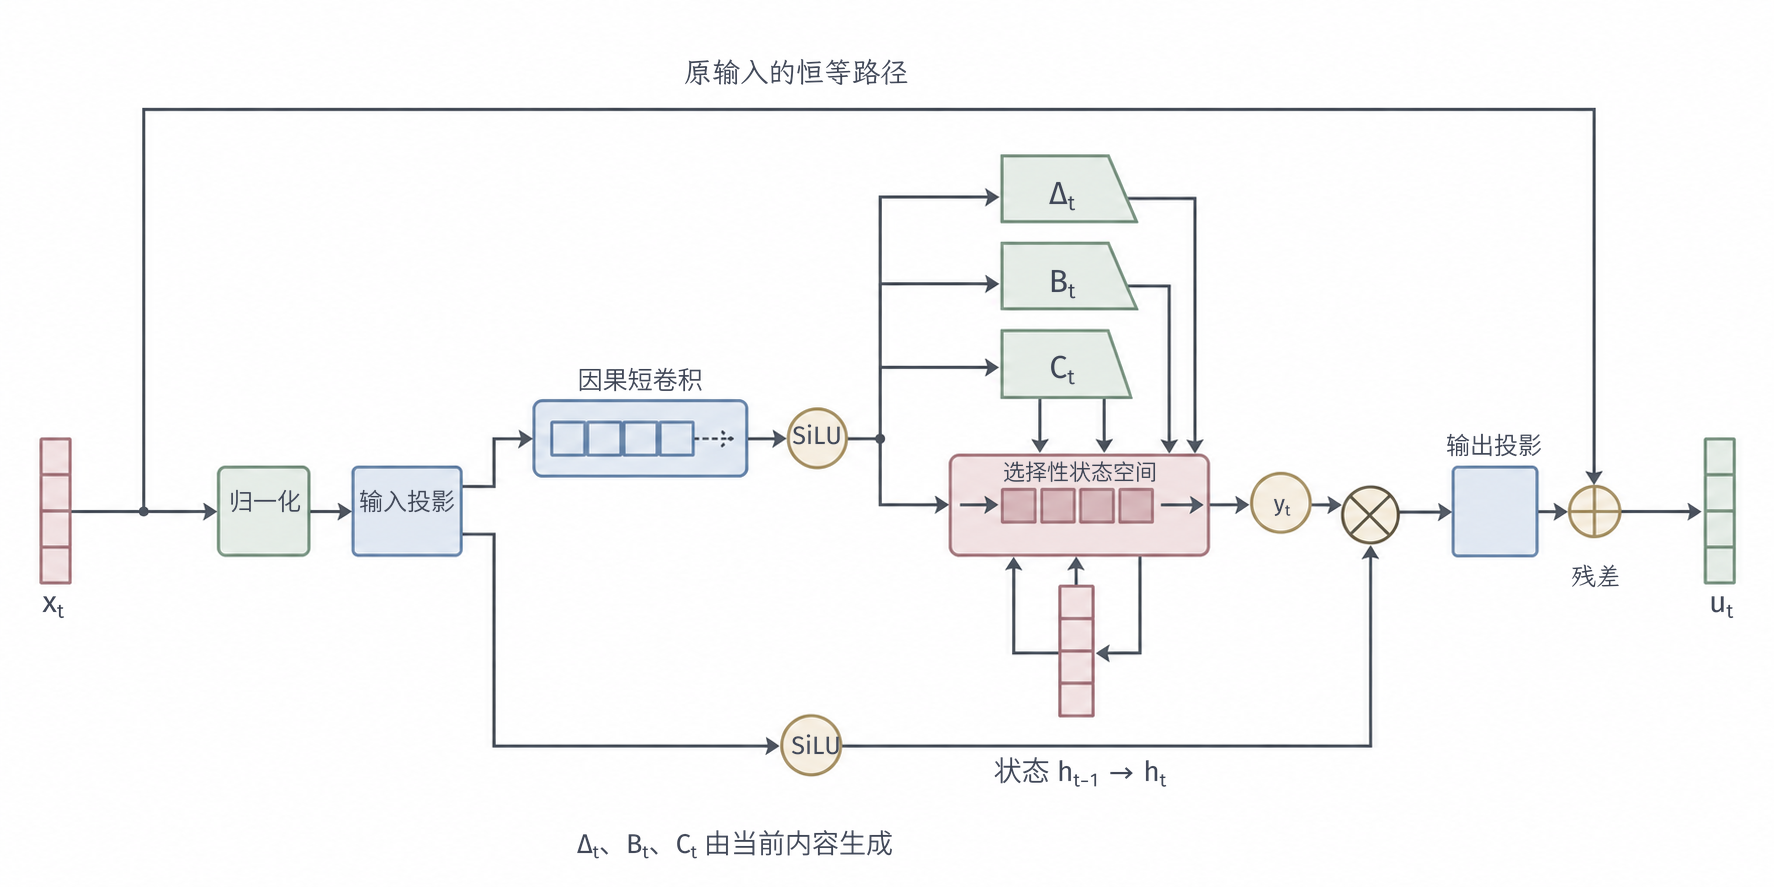
\includegraphics[width=150.199mm]{figures/03-models/02-neural-network-models/generated/rnn-mamba/figure.png}
  \caption{原始Mamba模块的主要计算路径。选择参数分支说明选择性的来源：短卷积后的输入特征生成$\Delta_t,\bm B_t,\bm C_t$，并据此调节SSM更新；另一路特征调制SSM输出，上方直达线完成跨层残差。$\bm u_t$是模块输出，任务预测由后续网络读出。图中省略短卷积缓存、批次维和跨通道广播细节。}
  \label{fig:rnn-mamba}
\end{figure*}

令归一化输入为$\widetilde{\bm x}_t\in\mathbb R^d$，内部通道数为$d_{\mathrm{in}}$，可将这两条支路写为
\begin{equation}
  \begin{aligned}
    \bm v_t&=\operatorname{SiLU}\!\left(\operatorname{CausalConv}
                (\bm W_{\mathrm v}\widetilde{\bm x})_t\right),\\
    \bm z_t&=\operatorname{SiLU}(\bm W_{\mathrm z}\widetilde{\bm x}_t),\\
    \bm y_t&=\operatorname{SelectiveSSM}(\bm v_{1:t}),\\
    \bm u_t&=\bm x_t+\bm W_{\mathrm{out}}(\bm y_t\odot\bm z_t)\text{。}
  \end{aligned}
  \label{eq:rnn-mamba-block}
\end{equation}
$\bm W_{\mathrm v},\bm W_{\mathrm z}\in\mathbb R^{d_{\mathrm{in}}\times d}$，$\bm W_{\mathrm{out}}\in\mathbb R^{d\times d_{\mathrm{in}}}$。各通道的选择系数由$\bm v_t$产生，$\bm y_t,\bm z_t$均为内部通道向量。SiLU调制支路缩放本步输出，其系数并未限制到$[0,1]$；时间记忆的保留率则来自SSM中的步长与状态参数。短卷积补充局部上下文，残差提供层方向的直达路径，各自作用不同。

\subsubsection{扫描、学习与计算代价}
\label{sec:rnn-mamba-scan}

输入相关系数使响应依赖具体输入和绝对位置，一般不能继续使用一个固定卷积核。不过，整段输入给定后，各步系数可先从输入计算；状态更新对旧状态仍是仿射的，对角结构又使组合便宜，所以能够使用式\eqref{eq:rnn-affine-composition}的扫描。若系数还依赖尚未算出的旧状态，就不能直接套用这种预先形成各步变换的方式，这也是它与一般LSTM／GRU计算组织的差别。

硬件感知的选择性扫描把离散化与状态更新放在适当存储层次中计算，避免在较慢存储中显式写出所有通道、所有位置的扩展状态；反向时可以重算中间量。扫描与重算改变计算顺序和存储策略，任务损失仍对同一递推求导。输入输出投影、短卷积、选择映射、状态参数与步长参数共同学习，选择哪些输入不是人工指定的必然结果。

设内部通道数为$d_{\mathrm{in}}$、每通道状态宽度为$m$，状态更新工作量为$O(Td_{\mathrm{in}}m)$，逐步持久状态为$O(d_{\mathrm{in}}m)$，还需短卷积和移位缓存。通道投影另有每步$O(dd_{\mathrm{in}})$成本。定长预测状态与高效整段扫描降低了计算负担，训练仍需优化器状态和相应反向信息，因此训练存储还随反向图、重算策略和优化器配置变化。

\subsubsection{有效时间与长期保留}
\label{sec:rnn-mamba-long-memory}

固定输入产生的系数，跨步状态扰动沿齐次路径传播为
\begin{equation}
  \frac{\partial\bm h^{(t)}}{\partial\bm h^{(s)}}
    =\exp\!\left(\bm A\sum_{u=s+1}^{t}\Delta_u\right)\text{，}
  \label{eq:rnn-mamba-memory-product}
\end{equation}
因为同一对角矩阵的指数可以相乘后合并。传播尺度由累计的内部步长决定：遇到无关输入时，若模型产生小$\Delta_u$，经过很多位置也可以只积累较少衰减；需要更新时再加大步长，并通过$\bm B_u$写入新内容。这将固定的逐步衰减变成内容相关的“有效经过时间”。

仍用式\eqref{eq:rnn-mamba-gate-special-case}作构造例子：从零状态读入$x_1=1$，取$\Delta_1=\log2$，得到$h^{(1)}=1/2$。其后100步输入为零且步长均为$0.001$，末状态为$(1/2)e^{-0.1}\approx0.452$。这个例子展示小步长如何弱化中间位置的遗忘；真实任务还要学到哪些位置应如此处理，且写入项的大小同时受$\bm B_t$和输入影响。

选择性更新把历史概括为定长状态。$\bm C_t$读取这些状态坐标，逐位置注意力则另存过去表示供本次查询评分；状态容量、输入干扰与有限精度仍限制可区分历史。系数对输入的导数、层间非线性和调制支路也进入完整梯度。选择机制提供了保留和覆盖的自由，扫描使这种机制便于计算，实际长期读取能力由保留规则、有限状态容量与任务学习共同决定。

% 完整作者列表较长，保留足够空间容纳本节开头的边注文献。
\Needspace{105mm}
\subsection{RWKV}
\label{sec:rnn-rwkv}

还可以用加权累积状态概括历史。\term{接收门加权键值网络}（receptance weighted key value, RWKV）以时间混合和通道混合构成模块，历史值由内容权重与时间衰减共同累积，再由接收门控制输出。本节采用2023年论文中的RWKV-4形式；后续版本的状态形状和更新可能不同\scite{peng2023rwkv}

\subsubsection{时间混合与加权状态}
\label{sec:rnn-rwkv-time-mixing}

设时间混合子模块的输入为$\bm{x}_t\in\mathbb{R}^{d}$，在完整层中它已由\term{层归一化}（layer normalization, LN）得到。这里LN只对同一位置的$d$个特征坐标计算均值与方差，标准化后再作可学习的逐坐标缩放和平移，各位置共享这些参数；具体公式见式\eqref{eq:transformer-layernorm}。它不跨样本或时间位置统计，因此归一化本身不会读取未来输入。时间混合先在当前与前一步输入之间逐坐标混合，再投影为键、值和接收向量：
\begin{equation}
  \bm{a}_t=\bm{W}_{\mathrm{a}}\!\left(
    \bm{\mu}_{\mathrm{a}}\odot\bm{x}_t
    +(\bm{1}-\bm{\mu}_{\mathrm{a}})\odot\bm{x}_{t-1}\right),
  \quad \mathrm{a}\in\{\mathrm{k},\mathrm{v},\mathrm{r}\}\text{。}
  \label{eq:rnn-rwkv-time-mixing}
\end{equation}
其中$\bm{\mu}_{\mathrm{a}}\in\mathbb{R}^{d}$是可学习混合系数，$\bm{W}_{\mathrm{a}}\in\mathbb{R}^{d\times d}$；$\bm{k}_t,\bm{v}_t,\bm{r}_t$分别取$\bm{a}_t$的对应结果。序列起始时的前一步输入需按约定初始化。

所有指数、除法和乘积按坐标进行。令非负衰减参数为$\bm{w}\in\mathbb{R}^{d}$，当前项偏置为$\bm{u}\in\mathbb{R}^{d}$，历史分子和分母状态初值为零，则
\begin{equation}
  \begin{aligned}
    \bm{v}_{\mathrm{agg}}^{(t)}&=
      \frac{\bm{a}^{(t-1)}+e^{\bm{u}+\bm{k}_t}\odot\bm{v}_t}
           {\bm{b}^{(t-1)}+e^{\bm{u}+\bm{k}_t}},\\
    \bm{a}^{(t)}&=e^{-\bm{w}}\odot\bm{a}^{(t-1)}
                    +e^{\bm{k}_t}\odot\bm{v}_t,\\
    \bm{b}^{(t)}&=e^{-\bm{w}}\odot\bm{b}^{(t-1)}+e^{\bm{k}_t},\\
    \bm{o}_t&=\bm{W}_{\mathrm{o}}\!\left(
      \operatorname{sigmoid}(\bm{r}_t)\odot\bm{v}_{\mathrm{agg}}^{(t)}\right)\text{。}
  \end{aligned}
  \label{eq:rnn-rwkv-recurrence}
\end{equation}
输出在历史状态更新前读取旧累积量，并为当前项使用$\bm{u}$；之后写入状态的当前项不包含该偏置。展开分子可见，第$i<t$个位置的权重为$\exp(-(t-1-i)\bm{w}+\bm{k}_i)$。它取决于该位置的键和时间距离，接收门再决定每个通道输出多少，没有对每个历史位置重新计算查询—键点积。

状态递推证明了过去的加权和可以由两个向量维护，不必逐步保存全部键值。直接指数形式容易上溢，实际实现还维护尺度或最大值，使用重缩放保持与上述比值等价。分母在非空步由正指数项保证为正；数值实现需要这种重缩放来控制指数范围。

\subsubsection{通道混合与完整残差层}
\label{sec:rnn-rwkv-architecture}

时间混合负责历史累积，\term{通道混合}（channel mixing）则在当前表示中组合不同特征。它也用当前与前一步输入作混合，但不重复WKV的历史加权和。令相应子模块输入仍记为$\bm x_t\in\mathbb R^d$，可写为
\begin{equation}
  \begin{aligned}
    \bm k'_t&=\bm W'_{\mathrm k}\left(\bm\mu'_{\mathrm k}\odot\bm x_t
          +(\bm1-\bm\mu'_{\mathrm k})\odot\bm x_{t-1}\right),\\
    \bm r'_t&=\bm W'_{\mathrm r}\left(\bm\mu'_{\mathrm r}\odot\bm x_t
          +(\bm1-\bm\mu'_{\mathrm r})\odot\bm x_{t-1}\right),\\
    \bm o'_t&=\operatorname{sigmoid}(\bm r'_t)\odot
         \bm W'_{\mathrm v}\left(\operatorname{ReLU}(\bm k'_t)
                              \odot\operatorname{ReLU}(\bm k'_t)\right)\text{。}
  \end{aligned}
  \label{eq:rnn-rwkv-channel-mixing}
\end{equation}
若内部宽度为$d_{\mathrm{ff}}$，则$\bm W'_{\mathrm k}\in\mathbb R^{d_{\mathrm{ff}}\times d}$、$\bm W'_{\mathrm v}\in\mathbb R^{d\times d_{\mathrm{ff}}}$，$\bm W'_{\mathrm r}\in\mathbb R^{d\times d}$。平方ReLU提供非线性通道变换，接收门调节其输出。混合系数是可学习参数，若没有额外约束，不保证它们一直处于$[0,1]$。

图~\ref{fig:rnn-rwkv}先给出完整残差层，再用虚线把时间混合子模块A与其内部计算对应起来。下方的输出$\bm o_t$就是上方A送入第一个残差加法的量；通道混合B随后处理更新的表示。在完整层公式中，$\bm x_t$改指归一化之前的层输入，$\bm s_t$表示第一次残差相加后的中间量，区别于WKV中的值向量$\bm v_t$。典型的归一化与残差关系为
\begin{equation}
  \begin{aligned}
    \bm s_t&=\bm x_t+\operatorname{TimeMix}
                    (\operatorname{LN}_1(\bm x_t)),\\
    \bm u_t&=\bm s_t+\operatorname{ChannelMix}
                    (\operatorname{LN}_2(\bm s_t))\text{。}
  \end{aligned}
  \label{eq:rnn-rwkv-residual-layer}
\end{equation}
LN是逐位置层归一化，状态更新在各子模块内部进行。时间混合与通道混合分别缓存各自归一化后进入子模块的前一步输入；两份缓存对应不同阶段的表示。完整生成网络在嵌入之后堆叠这些层，再用归一化和词表投影形成下一词元的概率。
\begin{figure*}[p]
  \centering
  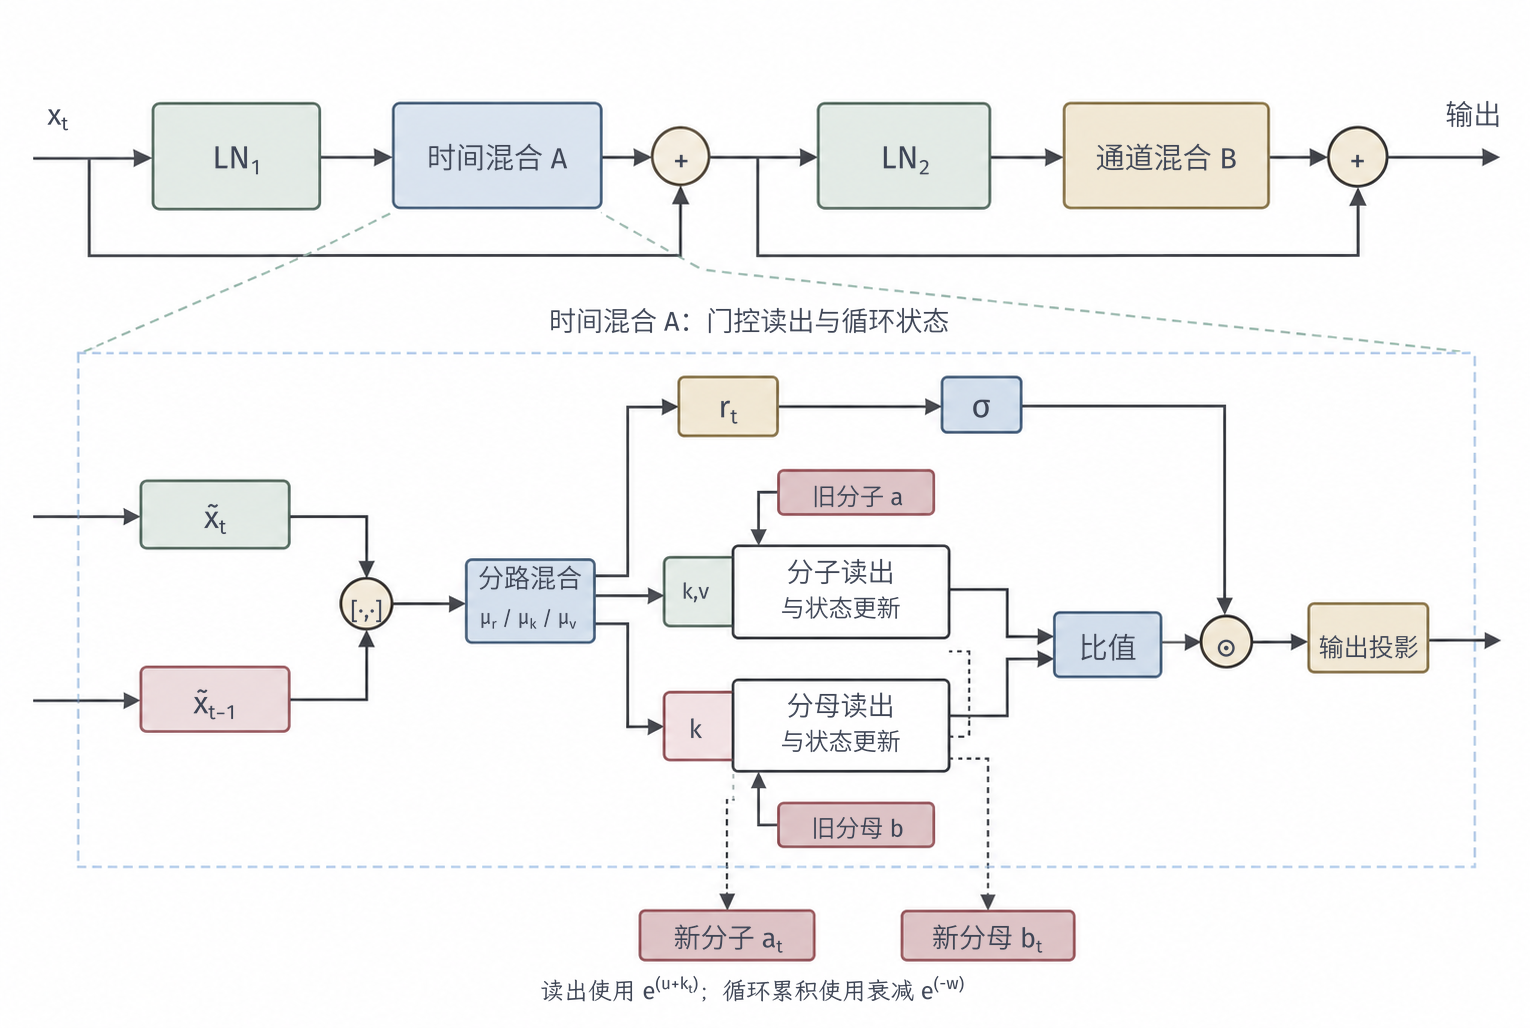
\includegraphics[width=129.540mm]{figures/03-models/02-neural-network-models/generated/rnn-rwkv/figure.png}
  \caption{RWKV-4的完整残差层与时间混合子模块。上方在A、B之前分别归一化，并在各子模块之后作残差相加，第一次相加得到$\bm s_t$。下方只展开A，无箭头虚线表示对应关系；$\widetilde{\bm x}_t=\operatorname{LN}_1(\bm x_t)$是归一化后的特征。左下圆圈将当前与前一步的归一化输入打包为有序对，不把它们相加；分路混合分别采用$\bm\mu_r$、$\bm\mu_k$、$\bm\mu_v$，再形成各自的投影。下方展开分子、分母状态与读出之间的关系：循环更新使用$e^{-\bm w}$衰减，读出中另含当前键的$e^{\bm u+\bm k_t}$权重；精确递推见正文公式。图中省略稳定化重缩放、移位缓存的保存箭头及B的内部计算。}
  \label{fig:rnn-rwkv}
\end{figure*}

训练时，各位置的稠密投影可以批量计算，WKV核心仍处理有序累积；可使用顺序扫描，满足组合条件时也可采用并行前缀计算。投影、混合系数、衰减及门由任务损失共同更新。逐步预测则只延续累积、移位与数值尺度状态。按$d$个通道计，累积核心整段为$O(Td)$、持久状态为$O(d)$，稠密投影另有每步$O(d^2)$或$O(dd_{\mathrm{ff}})$成本；层数、词表与训练反向信息需另外计算。

\subsubsection{归一化权重与长期依赖}
\label{sec:rnn-rwkv-long-memory}

RWKV没有在累积状态上反复施加普通RNN的稠密非线性变换，旧贡献沿各通道按$e^{-w_i}$保留。较小的$w_i$提供较长时间尺度，较大的值强调近期；内容键再改变各位置写入的权重。对固定键与衰减，某个历史值坐标对当前聚合的直接系数是归一化权重：
\begin{equation}
  \frac{\partial v_{\mathrm{agg},j}^{(t)}}{\partial v_{i,j}}
     =\frac{\exp(-(t-1-i)w_j+k_{i,j})}
       {b_j^{(t-1)}+\exp(u_j+k_{t,j})},\qquad i<t\text{。}
  \label{eq:rnn-rwkv-value-gradient}
\end{equation}
它取决于内容与时间距离，不是一个任意非线性状态Jacobian矩阵的连乘。完整任务梯度还包含接收门、输出投影以及键变化的路径，并受归一化权重的尺度影响。

归一化约束了加权聚合的范围，却不取消遗忘。若$w_j>0$，早期权重仍会随距离指数减弱；即使$w_j=0$、所有键相同且当前偏置为零，单个位置的权重也会随位置数按$1/t$稀释。较大内容权重可以让某些位置更突出，但并未建立对每个历史位置重新执行查询的机制。

压缩还会合并不同历史。例如只看一个$w=0$、全部键为零的累积核心，值序列$(1,0,0)$与$(0,1,0)$都产生分子1、分母3。它们的位置不同，两个累积量却相同；只依据这组状态无法区分证据曾出现在哪一步。多通道、移位和深层非线性增加了可用表示，但仍需依据具体任务检查压缩后的可区分性。

RWKV因此用内容加权、可学习衰减和接收门组织可延续的历史，使训练投影便于批量计算、预测状态保持定长。它缓解了一部分普通非线性循环路径的困难，保留范围与检索能力仍由时间尺度、写入权重、层间计算和任务监督共同决定。

表~\ref{tab:rnn-state-models}统一比较上述状态模块。HiPPO是一套状态构造原则，S4、Mamba和RWKV是利用特定结构组织序列计算的网络设计，比较时分别记录状态构造原则、实际网络更新与计算组织，便于看出它们的组合关系。

\begin{table*}[htb]
  \small
  \begin{tabularx}{\linewidth}{@{}p{19mm}XXX@{}}
    \toprule
    模型或原则 & 历史表示与选择 & 整段计算 & 逐步持久状态 \\
    \midrule
    普通RNN & 非线性隐藏状态；全部坐标经共同更新 & 时间递推与BPTT & 单层$m$维状态 \\
    LSTM／GRU & 门调节保留和写入；LSTM另有记忆状态 & 通常逐步递推 & 等宽LSTM为$2m$，GRU为$m$ \\
    HiPPO & 基函数系数；测度与阶数决定近似范围 & 取决于所选更新与离散化 & $m$个投影系数 \\
    S4 & 结构化线性状态；固定时间响应 & LTI模块可用结构核与FFT卷积 & 每通道$m$维状态 \\
    Mamba & 输入相关步长、写入与读出 & 选择性仿射扫描 & $d$通道共$dm$维状态，另有短卷积缓存 \\
    RWKV-4 & 内容加权累积、时间衰减与接收门 & 批量投影和加权扫描等 & 两组累积向量及移位、数值尺度缓存 \\
    \bottomrule
  \end{tabularx}
  \caption{历史压缩与计算方式的比较。这里$m$表示状态宽度，$d$表示通道数，均按单层比较；持久状态只计流式预测中需延续的信息，不含参数、输出缓存和反向传播激活。稠密投影、层数与数值实现会改变完整网络的计算和存储。}
  \label{tab:rnn-state-models}
\end{table*}

定长状态的代价不随已读长度线性增加，但相同宽度并不意味着相同的信息容量。循环注意力保存各位置编码状态，付出随输入长度增长的存储与读取；压缩状态把这一要求转为历史如何概括。两类模型的取舍应结合任务所需的精确位置访问、预测延迟和输入范围判断。

\section{循环神经网络的扩展}
\label{sec:rnn-extensions}

此前主要沿一条时间链组织状态。实际任务还会改变两个方向：信息可以沿不同拓扑传递，同一位置也可以经过多层表示变换。前者通过前驱关系决定一个状态看得到哪些对象，后者安排同一位置的层间表示变换。

\subsection{支持不同的拓扑结构}
\label{sec:rnn-topologies}

\subsubsection{双向循环与信息可见范围}
\label{sec:rnn-bidirectional}

离线词语标注可以利用整段文字，单向状态却只看到当前位置及此前输入。\term{双向循环网络}（bidirectional RNN）分别沿正向和反向读取同一输入，再把同一位置的两组状态组合：
\begin{equation}
  \begin{aligned}
    \overrightarrow{\bm{h}}^{(t)}&=F_{\rightarrow}\!\left(
       \overrightarrow{\bm{h}}^{(t-1)},\bm{x}_t\right),\\
    \overleftarrow{\bm{h}}^{(t)}&=F_{\leftarrow}\!\left(
       \overleftarrow{\bm{h}}^{(t+1)},\bm{x}_t\right),\\
    \bm{h}_t&=[\overrightarrow{\bm{h}}^{(t)};
                 \overleftarrow{\bm{h}}^{(t)}]\text{。}
  \end{aligned}
  \label{eq:rnn-bidirectional}
\end{equation}
两向通常使用不同参数，分别从序列两端的初态开始。反向上标$(t)$仍对齐输入位置，计算次序却是$T,T-1,\ldots,1$。两条链在同一步不必互相反馈，组合后的表示交给读出或下一层。

双向表示能使用后文，前提是后文在预测时已经可见。实时下一步预测若把尚未到达的观测送入反向链，就泄漏了未来信息；整段编码器用于转换任务则可以合法读取完整源序列。预测时已知哪些输入，决定了当前状态可采用哪一条信息路径。

\subsubsection{多维与多方向循环}
\label{sec:rnn-multidimensional}

规则网格中的当前位置可以依赖多个已计算的邻居。\term{多维循环网络}（multi-dimensional RNN）沿网格上的有向顺序组合这些前驱状态。例如二维网格的一个方向可采用
\begin{equation}
  \bm{h}_{i,j}=\tanh\!\left(
     \bm{U}\bm{x}_{i,j}+\bm{W}_1\bm{h}_{i-1,j}
      +\bm{W}_2\bm{h}_{i,j-1}+\bm{b}\right)\text{。}
  \label{eq:rnn-multidimensional}
\end{equation}
网格边界上的缺失前驱按约定初始化。该方向只读取上方和左方已形成的表示；按$i+j$分组时，同一对角线的节点可并行，而后续对角线依赖此前结果。再以其他角落为起点建立多个方向，就能组合不同象限的上下文\scite{graves2007mdrnn}

这里的多方向不是对同一条序列多跑几次，而是改变前驱关系。梯度沿多个前驱分支回传，对共享参数累积所有位置的贡献。直接把多路记忆相加还会增加状态幅度，门控、归一化和组合规则需随前驱数量设计；稳定性也要按新增前驱和完整组合规则分析。

\subsubsection{树递归与Tree-LSTM}
\label{sec:rnn-tree}

当输入已有语法树或层次结构时，相邻叶子未必就是最自然的组合对象。\term{树递归网络}（recursive neural network）按树的父子依赖组合状态：先得到子节点表示，再在父节点生成更大子结构的表示。名称中的recursive描述结构递归，与沿时间重复更新的recurrent口径不同，本章把二者都放在隐状态递推的框架下比较。

二叉树可以把左右子状态拼接后变换；子节点数不固定时，可以先求和聚合。\term{树结构长短期记忆}（Tree-LSTM）为每个子节点设置遗忘门，以不同权重组合其记忆。以Child-Sum版本为例，令$C(j)$是节点$j$的子节点索引集合，$\bm{x}_j$是本节点输入，$\bm{h}_j,\bm{c}_j$分别为隐藏和记忆状态，计算
\begin{equation}
  \begin{aligned}
    \overline{\bm{h}}_j&=\sum_{k\in C(j)}\bm{h}_k,\\
    \bm{i}_j&=\operatorname{sigmoid}\!\left(
       \bm{U}_{\mathrm{i}}\bm{x}_j+\bm{W}_{\mathrm{i}}\overline{\bm{h}}_j
       +\bm{b}_{\mathrm{i}}\right),\\
    \bm{o}_j&=\operatorname{sigmoid}\!\left(
       \bm{U}_{\mathrm{o}}\bm{x}_j+\bm{W}_{\mathrm{o}}\overline{\bm{h}}_j
       +\bm{b}_{\mathrm{o}}\right),\\
    \widetilde{\bm{c}}_j&=\tanh\!\left(
       \bm{U}_{\mathrm{c}}\bm{x}_j+\bm{W}_{\mathrm{c}}\overline{\bm{h}}_j
       +\bm{b}_{\mathrm{c}}\right),\\
    \bm{f}_{j,k}&=\operatorname{sigmoid}\!\left(
       \bm{U}_{\mathrm{f}}\bm{x}_j+\bm{W}_{\mathrm{f}}\bm{h}_k
       +\bm{b}_{\mathrm{f}}\right),\qquad k\in C(j),\\
    \bm{c}_j&=\bm{i}_j\odot\widetilde{\bm{c}}_j
        +\sum_{k\in C(j)}\bm{f}_{j,k}\odot\bm{c}_k,\\
    \bm{h}_j&=\bm{o}_j\odot\tanh(\bm{c}_j)\text{。}
  \end{aligned}
  \label{eq:rnn-tree-lstm}
\end{equation}
叶节点的空和为零，参数形状与等宽链式LSTM相同。求和对孩子的重编号不变，但会弱化孩子次序；若左右位置具有不同语义，采用带位置参数的有序树版本更合适。Tree-LSTM的代表工作分别讨论了这两类结构\scite{tai2015}

图~\ref{fig:rnn-topologies}将依赖范围与计算顺序并列展示。树上的反向传播从父节点回到各孩子，多个损失的贡献在同一节点汇合；共享组合参数的梯度再对所有节点累积。两个叶子经树组合到共同祖先的路径可以短于按词序遍历的路径，但这种优势依赖给定树是否符合任务，还增加了结构取得与处理的要求。

\begin{figure*}[t]
  \centering
  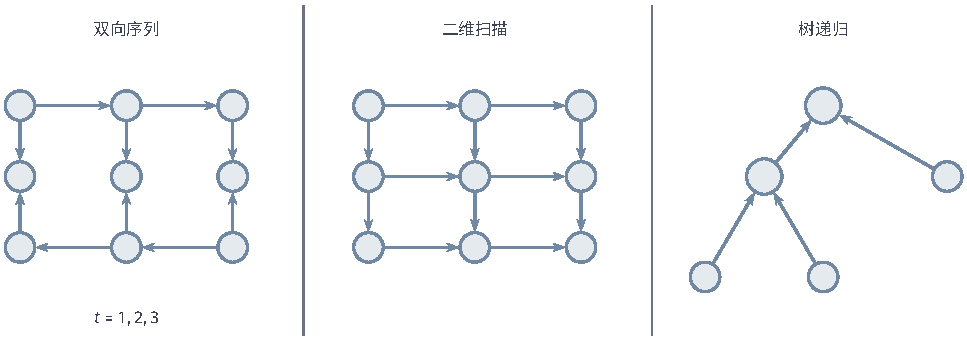
\includegraphics[width=163.791mm]{figures/03-models/02-neural-network-models/tikz/rnn-topologies/figure.pdf}
  \caption{状态依赖拓扑。左图在同一输入位置组合正向与反向状态；中图由上方、左方前驱形成二维状态，箭头给出一个扫描方向；右图由叶节点向父节点组合子结构。圆节点表示各位置或子结构的状态，箭头表示状态依赖的方向。不同方向、位置或孩子组合是否共享参数，需要由具体模型说明。}
  \label{fig:rnn-topologies}
\end{figure*}

\subsection{支持更深的网络}
\label{sec:rnn-depth}

时间展开的深度由序列长度决定，同一位置的表示变换深度则由层数决定。增加层数既可以让任务学习更多表示变换，也可以仅堆叠固定动态、提供更多历史特征。二者共享层次结构，却训练不同参数。

\subsubsection{堆叠循环网络：学习各层表示与时间动态}
\label{sec:rnn-stacked-networks}

\term{堆叠循环网络}（stacked RNN）让上层读取下层在相同位置的状态，同时维护自己的历史。设层数为$L$，$\bm h_0^{(t)}=\bm x_t$，则
\begin{equation}
  \bm h_{\ell}^{(t)}=F_{\ell}\!\left(\bm h_{\ell}^{(t-1)},
       \bm h_{\ell-1}^{(t)}\right),\qquad\ell=1,\ldots,L\text{。}
  \label{eq:rnn-stacked}
\end{equation}
上标是时间步，下标$\ell$是层索引。同一层跨步共享参数，不同层通常各用一组参数。单元可选普通RNN、LSTM或GRU；使用LSTM时，各层还维护自己的记忆状态$\bm c_\ell^{(t)}$。

第$t$步先计算底层，再把底层当前表示送到第二层，依次形成顶层表示。因而第二层同时读取“这一位置的底层特征”与“第二层此前形成的历史”。单向堆叠仍只使用当前及此前输入。

图~\ref{fig:rnn-stacked-network}展示三层网络的时间展开。水平箭头传递同层历史，垂直箭头传递同一时刻的层间表示。
\begin{figure}[htbp]
\centering
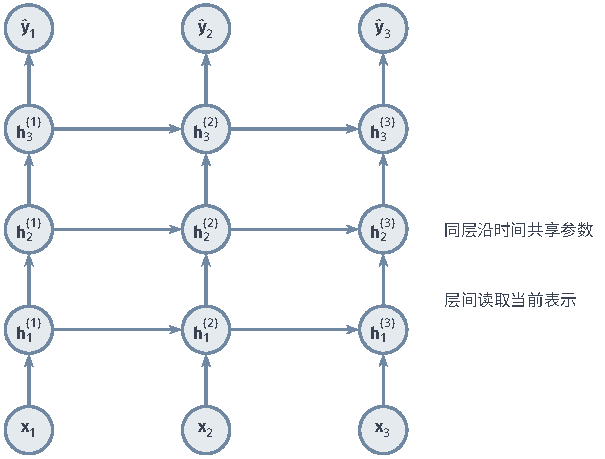
\includegraphics[width=102.369mm]{figures/03-models/02-neural-network-models/tikz/rnn-stacked-network/figure.pdf}
\caption{三层堆叠循环网络。每层具有自己的循环参数并沿时间共享；上层读取下层当前状态与自身上一时刻状态，输出由顶层状态形成。图省略初态和层内门控。}
\label{fig:rnn-stacked-network}
\end{figure}


任务损失通常从顶层读出，也可以拼接或加权读取多个层。训练时梯度既沿时间回传，也沿层间依赖回传，各层循环与输入映射都接受任务监督。下层可以形成较局部的表示，上层再组合这些表示，但各层的时间尺度由实际动态和输入驱动决定，可以通过状态响应或任务行为检验。

若第$\ell$层宽度为$m_\ell$、$m_0=d$，普通稠密单元的整段计算量级为
\begin{equation}
  O\!\left(T\sum_{\ell=1}^{L}m_\ell(m_{\ell-1}+m_\ell)\right)\text{，}
  \label{eq:rnn-stacked-cost}
\end{equation}
门控单元还增加相应常数。完整反向计算需保存或重算各层各步的激活。层宽、读出范围与训练存储因此都影响深度选择。

\subsubsection{深度储备池计算：堆叠固定动态、学习统一读出}
\label{sec:rnn-deep-reservoir}

\term{深度储备池计算}（deep reservoir computing）把多个通常固定的储备池按层连接，利用层层动态形成历史特征，再训练任务读出。深度ESN是代表形式，第一层读取外部输入，上层读取下层当前状态\scite{gallicchio2018deepesn}

对泄漏积分单元，可写为
\begin{equation}
  \begin{aligned}
    \bm h_\ell^{(t)}&=(1-\alpha_\ell)\bm h_\ell^{(t-1)}
      +\alpha_\ell\tanh\!\left(\bm W_\ell\bm h_\ell^{(t-1)}
               +\bm U_\ell\bm h_{\ell-1}^{(t)}+\bm b_\ell\right),\\
    \widehat{\bm y}_t&=g\!\left(\bm V
       [1;\bm x_t;\bm h_1^{(t)};\ldots;\bm h_L^{(t)}]\right)\text{。}
  \end{aligned}
  \label{eq:rnn-deep-esn}
\end{equation}
$0<\alpha_\ell\leq1$是各层泄漏率，$\bm W_\ell,\bm U_\ell,\bm b_\ell$按构造固定，$\bm V$是可训练读出矩阵；也可以只读部分层。训练先逐步收集拼接特征，再拟合读出，平方损失时仍是一组扩展特征上的岭回归，不需要为固定循环参数执行任务梯度更新。

层叠改变输入经过的动态过滤。在线性标量简化且循环矩阵为零时，$h^{(t)}=(1-\alpha)h^{(t-1)}+\alpha u_t$，记忆按$(1-\alpha)^k$衰减，对$0<\alpha<1$的时间尺度为$-1/\log(1-\alpha)$。这说明不同泄漏率可以提供不同更新速度；真实储备池还包含反馈矩阵、输入驱动与非线性，整个模型的时间响应由这些因素共同形成。

各层也要检查回声状态性质。设相同输入下的两条轨迹距离为$\delta_\ell^{(t)}$，Tanh的Lipschitz性质给出
\begin{equation}
  \delta_\ell^{(t)}\leq r_\ell\delta_\ell^{(t-1)}
       +\alpha_\ell\lVert\bm U_\ell\rVert_2\delta_{\ell-1}^{(t)},
  \quad r_\ell=1-\alpha_\ell+\alpha_\ell\lVert\bm W_\ell\rVert_2\text{。}
  \label{eq:rnn-deep-esn-contraction}
\end{equation}
外部输入相同时$\delta_0^{(t)}=0$。有限层数、各$r_\ell<1$且层间映射有界时，下层初态差异逐渐消失，上层受其驱动的差异也能衰减。这是充分条件；上述推导把各层收缩与层间有界映射共同计入，整个层叠的初态遗忘由这一组合条件支持。

与可训练堆叠RNN相比，深度储备池减少了循环动态的优化范围，多个层的特征可供同一读出选择；代价是固定状态变换不能按任务梯度重新安排记忆。层数、宽度、连接尺度和泄漏率通常由验证过程选择，测试数据不能参与这种选择。更多固定层可能增加有用时间特征，也可能增加冗余或压缩损失，需要与浅层储备池在相近预算下比较。

\subsubsection{跨层连接与分层读出}
\label{sec:rnn-depth-connections}

可训练网络与固定储备池都可以改变层间连接。维度相同时，跨层残差可写为$\bm u_\ell^{(t)}=\bm h_{\ell-1}^{(t)}+G_\ell^{(t)}$，其中$G_\ell^{(t)}$是这一层产生的变换结果；维度不同时先投影直达分支。残差为层方向提供较直接的梯度路径，通常没有缩短同一层的时间路径。

分层读出把不同层的状态送到任务头，使监督或读出可以直接使用多个层次的特征；它扩大了读出输入与参数规模。跨时间跳跃、跨层残差和门控可以组合；连接的起止状态与可训练参数确定各自的依赖路径。层深安排表示组合，时间尺度安排历史保留，读出范围安排任务访问。

\section{理论分析}
\label{sec:rnn-theory}

结构提供了可用的信息路径，仍需考察学习能否改进目标，以及有限训练数据能否支持新序列上的预测。以下分别分析表达能力、参数优化与预测风险，承接机器学习理论部分的工具；状态递推是否稳定作为影响条件出现，不与参数优化的收敛混为一谈。

\subsection{表达能力}
\label{sec:rnn-expressivity}

循环网络用固定宽度状态概括历史；能否拟合目标取决于这个状态是否保留预测所需信息。若两段历史进入相同状态，面对相同后缀与读出时就无法给出不同答案。计数、短期模式或有限状态任务可能适合紧凑递推，依赖任意历史细节的查询则可能要求更宽状态、外部读取或更长的传播路径。

门控改变哪些信息持续保存，堆叠改变每一步可组合的非线性变换。它们扩大或重组候选函数，却不保证任意长度目标都能在固定宽度和有限精度下实现。存储能力还受噪声、精度和连续性条件限制；无限精度实数状态与有限精度设备对应不同的可区分状态数。

\subsection{收敛性}
\label{sec:rnn-convergence}

训练收敛描述参数更新过程，状态稳定性描述给定参数下的输入响应。Tanh使隐藏坐标有界，状态对参数的导数仍经过多步Jacobian矩阵乘积；持续变化的输入又可以使已训练模型的状态持续变化。

对固定训练集、有限长度序列和确定的初始化规则，完整BPTT给出训练目标$L(\bm{\theta})$的精确梯度。假设在迭代所处区域内$L$可微、梯度为$\beta$-Lipschitz且$L\geq L_{\inf}$，采用固定步长$0<\eta\leq1/\beta$更新。下降引理给出
\begin{equation}
  L(\bm{\theta}^{(k+1)})
    \leq L(\bm{\theta}^{(k)})
       -\frac{\eta}{2}\lVert\nabla L(\bm{\theta}^{(k)})\rVert_2^2\text{，}
  \label{eq:rnn-descent}
\end{equation}
这里$(k)$是参数更新轮次，与状态时间步$(t)$分开。将$K$次不等式相加得到
\begin{equation}
  \frac{1}{K}\sum_{k=0}^{K-1}
     \lVert\nabla L(\bm{\theta}^{(k)})\rVert_2^2
     \leq\frac{2\left(L(\bm{\theta}^{(0)})-L_{\inf}\right)}{\eta K}\text{。}
  \label{eq:rnn-stationarity}
\end{equation}
这个结论保证平均平方梯度随迭代次数变小，涉及趋近一阶驻点；该指标控制已计算迭代点的梯度尺度，全局最优与参数序列的极限还需其他条件。非光滑激活、随机梯度、裁剪或自适应优化改变了梯度或更新规则，其结论据相应条件另行建立。

循环结构会改变假设中的常数。状态对参数的一阶、二阶敏感度包含跨步传播，长序列与放大动态可能使允许的步长变小。较小梯度也可能来自早期路径消失，而不是目标已经满意；因此，梯度范数与训练误差需要同时解释。正交约束作用于线性部分，门控提供选择性路径，跳跃连接改变传播距离，但这些机制改变的是完整非凸目标中的部分传播条件。

截断BPTT还改变了梯度对象。将所用梯度写成$\widetilde{\bm{g}}=\nabla L+\bm{e}$，误差$\bm{e}$进入下降项$\langle\nabla L,\widetilde{\bm{g}}\rangle$，因而式\eqref{eq:rnn-descent}不再自动成立。若跨步状态Jacobian矩阵统一收缩且局部导数有界，被切断的远期贡献可由几何尾和控制；当长期保留的路径接近不衰减时，短截断就可能遗漏显著贡献。

这种遗漏不只是代价分析中的常数。若某参数只在首步读入证据时起作用，损失仅在很晚的末步出现，把中间状态断开后，该参数对当前片段损失的梯度可以为零，而完整梯度仍非零。前向状态可把证据带到末步，跨边界的反向路径才把末步损失传给形成证据表示的参数。

储备池把循环参数固定后，平方损失读出可转为式\eqref{eq:rnn-esn-ridge}的凸二次问题。$\lambda>0$时该问题具有唯一解，可以直接求解，也可以在适当步长下迭代。这个结论只覆盖给定状态特征的读出优化，不覆盖储备池超参数选择或整个模型的预测质量。结构化状态网络同样需要区分可高效计算梯度与优化目标具有何种收敛保证。

\subsection{泛化性}
\label{sec:rnn-generalization}

先明确一个训练样本是什么。对独立评论分类，可以把整段评论及标签视为一个样本；对多个独立设备的数据流，也可以把每条按约定长度取得的序列视为样本。一个序列中有$T$个位置，不代表有$T$个独立训练样本。若只是同一条长流的重叠窗口，样本间相关，独立同分布结论需要相应依赖分析后才能使用。

设$\mathcal{F}$是限定结构、参数范围和输入长度后的预测函数族，$\bm{Z}_1,\ldots,\bm{Z}_n$为独立同分布的完整序列样本；$\bm{Z}$包含输入及相应目标。记有界损失为$\ell(f,\bm{Z})\in[0,1]$，风险为$R(f)=\mathbb{E}[\ell(f,\bm{Z})]$，经验风险为$\widehat R_n(f)=n^{-1}\sum_i\ell(f,\bm{Z}_i)$。对预先固定的有限候选族，Hoeffding不等式与并合界给出，以至少$1-\delta$的概率，
\begin{equation}
  \sup_{f\in\mathcal{F}}\left|R(f)-\widehat R_n(f)\right|
    \leq\sqrt{\frac{\log(2|\mathcal{F}|/\delta)}{2n}}\text{。}
  \label{eq:rnn-finite-family-bound}
\end{equation}
统一界允许模型依据这些训练样本从候选中选择；$n$仍是独立序列数。无界交叉熵超出了这里的$[0,1]$条件；分析它时可另加预测概率下界、截断损失或尾部条件，并建立对应的风险界。

连续参数族中的函数数目一般无限，式中$|\mathcal{F}|$需要由有限覆盖等量替换。可以使用覆盖数、Rademacher复杂度或算法稳定性，具体依赖由任务和约束决定。若在全部允许样本上有一个有限的损失$\varepsilon$-覆盖，式\eqref{eq:rnn-finite-family-bound}可用于覆盖代表，并增加至多$2\varepsilon$的近似项。覆盖规模取决于参数范围及参数变化对输出的影响，循环敏感度由此进入泛化分析。

输入尺度和长度怎样影响敏感度，可以在普通单元上直接计算。假设初态为零、$\lVert\bm{x}_t\rVert_2\leq B_x$，激活为1-Lipschitz且零点取零，$\lVert\bm{W}\rVert_2\leq r$，则
\begin{equation}
  \lVert\bm{h}^{(t)}\rVert_2
    \leq\left(\lVert\bm{U}\rVert_2 B_x+\lVert\bm{b}\rVert_2\right)
       \sum_{k=0}^{t-1}r^k\text{。}
  \label{eq:rnn-state-norm-bound}
\end{equation}
$r<1$时几何和有统一上界，$r=1$时按$t$增长，$r>1$时该上界可能快速增长。对Tanh还可使用$\sqrt m$的状态上界，取较紧者；状态有界却不意味着参数敏感度同样有界。

固定参数并扰动输入，由逐步Lipschitz性质还能得到
\begin{equation}
  \lVert\bm{h}^{(T)}-\widetilde{\bm{h}}^{(T)}\rVert_2
    \leq\lVert\bm{U}\rVert_2
      \sum_{t=1}^{T}r^{T-t}\lVert\bm{x}_t-\widetilde{\bm{x}}_t\rVert_2\text{，}
  \label{eq:rnn-input-sensitivity}
\end{equation}
其中两条序列初态相同。读出再乘以输出映射和损失的相应Lipschitz常数。它说明状态转移范数、输入尺度和长度怎样控制输入敏感度。$r>1$时这个上界较大，实际风险还取决于状态轨迹、函数族和数据。

结构也影响允许的函数族。隐状态维度、层数、双向或树状连接、门的参数，以及注意力的评分与读取范围，都会改变复杂度和信息约束。参数共享使参数数目不随长度增加，但共享参数在更长计算中的重复作用仍可能改变复杂度常数。注意力权重归一化约束了固定值向量的聚合范围，评分和编码表示的学习敏感度仍需计入；结构化状态更新减少某些自由度，也可能引入不符合数据的记忆假设。

\term{长度外推}（length extrapolation）考察测试序列超出训练长度范围时的预测。共享参数使网络能够运行在更长输入上，却没有保证其误差保持不变。训练中未见的依赖距离、计数规模、时间尺度和状态饱和都可能改变行为。固定维度的实数状态在无限精度的数学模型中与有限精度实现也不同，可区分的历史数量随精度和读取条件而变，需要在指定这些条件后讨论存储上限。

因此，泛化比较应固定预测任务、数据来源、独立样本单位、长度范围和参数预算。训练长度内的测试误差、跨长度表现与跨分布表现是不同问题；不同任务需要保留的信息与预测范围不同，各自的比较由这些共同条件建立。

\section{常见应用}
\label{sec:rnn-applications}

应用中的关键是把可见输入、输出含义、训练目标和预测时的状态延续对应起来。以下使用简单任务展示这一过程，具体语言、信号和生成方法留给应用卷。

\subsection{序列分类}
\label{sec:rnn-application-classification}

以评论情感分类为例，一个样本是整段评论和类别$y$。沿用第~\ref{sec:rnn-encoder-decoder}节的嵌入查表方式，将离散词元映射为$\bm{x}_t=\bm{E}_{:,v_t}$，其中$\bm{E}\in\mathbb{R}^{d\times K_{\mathrm{vocab}}}$，$v_t$是词表索引，再用RNN、LSTM或GRU编码。末状态或掩码平均形成整段表示，经Softmax分类头输出概率，训练时对独立评论的交叉熵取平均；嵌入、循环单元和分类头共同更新。

单向编码适合边读边更新状态，但如果目标是整段类别，预测仍需说明何时决定结果。双向编码在读到完整评论后利用前后上下文；两向沿不同顺序读取，概括全段的状态分别位于正向有效末位置和反向有效首位置；也可以聚合各位置的双向表示。评估时保持分词、有效长度和聚合规则一致。

评论中的“并不精彩”提示模型需要组合否定与后续词，而不是只累计正向词频。这个例子指出了任务需要保留的关系，模型是否学得由预测结果检验。验证样本用于选择宽度、聚合和停止轮次，未参与选择的测试样本再用于评价。

\subsection{序列标注与时间预测}
\label{sec:rnn-application-aligned}

词语标注把每个有效位置的表示送入分类头，按照式\eqref{eq:rnn-aligned-loss}计算交叉熵。离线标注可用双向上下文，流式标注只使用当前已可见输入，或明确约定等待若干后续位置的延迟。循环状态提供输入历史的表示，逐位置Softmax分别预测各标签；若任务还要求标签组合合法，可以另接体现这些约束的输出模型。

以设备温度预测为例，$\bm{x}_t$可包含当前温度、控制量和已知时间间隔，读完这一步后输出下一时刻的温度估计$\widehat x_{t+1}$。有效预测位置集合记为$V$，平方目标为
\begin{equation}
  \ell=\frac{1}{|V|}\sum_{t\in V}
      (\widehat x_{t+1}-x_{t+1})^2\text{。}
  \label{eq:rnn-forecast-loss}
\end{equation}
目标位移必须在构造样本时完成，预测时不能输入待预测值。归一化统计只从训练数据估计，划分沿实际预测时间或按独立设备进行，避免重叠窗口把同一未来观测泄漏到训练与测试两侧。

流式使用时，传入新观测、更新状态、输出预测，再等待下一观测。跨片段可以延续同一设备状态，训练中则按截断长度切断梯度；设备切换、重新启动或大段缺失后的重置规则需要与训练匹配。多步预测若反馈自己生成的数值，误差可能累积；若使用未来外部变量，只能输入预测时确已知道的部分。历史用于形成已有信息下的预测，未来外部条件是否已知则决定了不同的预测任务。

\subsection{序列转换与生成}
\label{sec:rnn-application-generation}

转换任务给定源序列，生成另一段目标序列。训练流程是编码源输入，给解码器输入BOS和真实目标前缀，以包含EOS的目标计算式\eqref{eq:rnn-sequence-likelihood}，再联合更新全部模块。带注意力时，同时保留有效编码状态及掩码，供各解码步读取。

预测流程中，源编码只需执行一次。解码器从初始状态和BOS开始，输出一个条件分布，按约定策略选择符号，将该符号嵌入送入下一步；遇到EOS或预设最大长度停止。最大长度限制了计算和输出，EOS则是模型产生的结束符号。束搜索分别维护各候选前缀的解码状态，使后续更新对应各自的生成历史。

单序列生成也可采用\term{自回归模型}（autoregressive model）：按已有前缀预测下一个符号，再把生成结果反馈为后续输入。源条件可省略或由其他输入提供，循环更新、教师强制和停止条件仍需明确。每步贪心、束搜索和采样采用不同的输出策略，生成结果及其评价随策略而变；采样的多样性与预测分布的可靠性分别检验。

\Needspace{85mm}
\section{本章小结}
\label{sec:rnn-summary}

输入陆续到达时，隐状态把此前计算带到当前，参数共享让同一更新规则适应不同长度。状态保留了什么，由更新、读出和任务监督共同决定。普通RNN将这套关系写成非线性递推，时间展开使梯度可以计算，也暴露了跨多步Jacobian矩阵乘积对长期学习的限制。

围绕同一历史依赖问题，储备池把动态构造与读出学习分开，控制门选择保留和写入，注意力通过保存各位置表示扩大可读取的信息。状态空间路线则利用可组合的状态更新，把部分整段计算改写为卷积或扫描。它们分别改变可训练参数、信息通路和计算形式，常可组合使用；预测状态规模、梯度路径和任务相关记忆分别由存储组织、依赖结构和信息保留决定。

拓扑决定预测时可见哪些输入，深度决定各位置经历怎样的表示变换。双向和多方向读取需要相应输入已经可见，树递归需要给定结构；跨层连接的作用也应与跨时间路径分清。优化下降的条件、独立序列样本数、输入尺度和训练长度范围共同约束学习结论，能执行更长递推不等于已经具备长度外推能力。

把这些模型用于具体任务时，需同时确定输入编码、监督位置、输出概率或数值含义，以及状态何时延续和重置。章首的历史依赖问题由此落实到完整过程：状态表示与读取机制把此前输入带入预测，损失通过依赖路径影响参数，再用具有相应信息范围的新序列检验结果。

\paragraph{扩展阅读}
Goodfellow等教材第10章讨论序列建模和循环计算，LSTM原论文把长期信用分配问题落实到状态与门的结构。前向记忆、反向梯度路径与训练样本单位在这些资料中对应不同的分析对象，分别说明历史保留、参数更新和预测风险的条件\scite{goodfellow2016,hochreiter1997}

\chapter{图神经网络}
\label{chap:graph-networks}

一个分子可以有不同数量的原子，每个原子连接的化学键也不一样；一篇论文的类别除了取决于正文，还可能与它引用的论文有关。这些输入既没有图像中整齐的网格，也没有序列中唯一的先后次序。按编号拼接原子属性时，换一种编号便会改变输入的排列；逐个处理原子时，化学键又没有进入计算。网络需要把原子与连接同时纳入，并让换编号只改变保存次序。本章要回答的问题是：网络怎样利用不规则的关系形成表示，同时让预测遵守对象重编号及任务本身的对称性？

关系参与预测，需要先确定每个对象能够读取哪些信息，再确定读取后怎样形成表示。节点从哪些邻居读取信息、怎样把数量可变的输入组合起来，决定一轮计算；传播多少轮、是否反复使用同一组参数，决定关系影响能够传多远。关系的类型、变化时间和几何含义又会约束消息的形式。消息传递给出节点、边和邻域之间的共同计算；图卷积与循环更新分别规定传播算子和参数复用。表示区分能力、传播行为及泛化条件，再说明这些计算在具体任务中能保留什么、怎样求值、需要何种数据证据。

\section{图神经网络概述}
\label{sec:gnn-overview}

前馈网络可以处理预先提取的分子描述向量，但描述向量中包含什么关系，取决于特征设计。卷积网络共享一个窗口内的计算，依赖网格中明确的相对位置；一般关系网络没有统一的“左上邻居”。循环网络能够读取一串对象，却需要额外规定遍历次序。序列化与固定特征也是可用表示；它们需要通过特征或遍历规则记录连接，并处理对象数量和排列变化。图网络则让输入关系直接决定对象之间的读取。

把原子、论文等对象记为节点，把它们之间的给定关系记为边。输入图为$\mathcal G=(V,E)$，$V=\{1,\ldots,n\}$，$e=|E|$。
节点$i$的属性为$\bm x_i\in\mathbb R^d$，消息边$j\to i$的属性记为$\bm a_{i,j}\in\mathbb R^{d_e}$。
消息下标先写接收者，再写发送者，与有向边的起点、终点记法分别使用。
分子属性可包含原子与键类型，引用网络的属性可包含论文内容（图对象的其他表示参考\BookSectionRef{sec:graph-theory-objects-representations}{第一卷“数学准备”的“图的对象与表示”节}）。

若有向邻接矩阵以行记起点、列记终点，本章为直接写出接收端汇总，使用其转置
$\bm A=\bm A_{\mathrm{graph}}^\top$，因此$\bm A_{i,j}$为$j\to i$的权重（邻接方向约定参考\BookSectionRef{sec:graph-theory-matrix-representations}{第一卷“数学准备”的“图的矩阵表示”小节}）。
$N(i)=\{j:\bm A_{i,j}\ne0\}$是发送有效消息的入邻域；
零权结构边若仍需参与计算，应另存结构掩码。无向图上矩阵对称，两种表示相同。
后文的谱域推导采用非负权重无向图，基础消息传递允许有向边。

\term{图神经网络}（graph neural network, GNN）让网络沿给定关系交换并组合对象的表示。它把“谁与谁相连”变成计算的组织依据，共享的更新规则则使同一网络可以处理不同节点数和邻居数。这里的图组织输入对象之间的计算；边的含义由原始关系给定，例如引用或化学键。条件独立性与因果作用需要各自的建模依据。

原子编号改变后，预测仍应对应原来的原子；分子的整体属性也应保持同一含义。令$\bm{X}\in\mathbb{R}^{n\times d}$按行存放节点特征，即$\bm{X}_{i,:}=\bm{x}_i^{\top}$；用\term{置换矩阵}（permutation matrix）$\bm{P}$重新排列这些行，则新的输入为$\bm{X}'=\bm{P}\bm{X}$、$\bm{A}'=\bm{P}\bm{A}\bm{P}^{\top}$，边属性也须同步重排。\term{置换等变性}（permutation equivariance）要求节点输出跟着节点一起重排；\term{置换不变性}（permutation invariance）要求整图输出保持不变。不含边属性时，两种要求可写为
\begin{equation}
  \begin{aligned}
    F(\bm{P}\bm{A}\bm{P}^{\top},\bm{P}\bm{X})
      &=\bm{P}F(\bm{A},\bm{X}),\\
    f(\bm{P}\bm{A}\bm{P}^{\top},\bm{P}\bm{X})
      &=f(\bm{A},\bm{X})\text{。}
  \end{aligned}
  \label{eq:gnn-permutation}
\end{equation}
$F$产生按节点排列的输出，$f$产生整图输出。重编号后，每个原子的预测仍对应同一个原子，分子的属性预测仍对应同一个分子；这里保持的是每个原子与其输出的对应，不同原子仍可有不同预测。

沿关系学习表示的思想早于今天的图卷积层。早期处理树和有向无环结构的递归网络，沿既定依赖逐步形成表示；一般图出现环时，邻居状态可能互相等待，需要给这一组依赖安排确定的求值方式。Gori等在2005年提出图神经网络模型，将节点状态定义为相互依赖方程的解，允许直接处理带环的图，并区分节点任务与整图任务\scite{gori2005graphdomains} Scarselli等在2009年的系统论述中，以共享局部更新和收缩条件保证状态解唯一，再通过反复更新求得稳定状态。共享更新把关系纳入表示，不动点求解处理环内依赖；所用收缩条件同时限定了更新函数的候选范围\scite{scarselli2009gnn}

另一条路线试图把卷积网络的共享滤波推广到不规则结构。Bruna等在2014年的Spectral CNN中，用图拉普拉斯的特征向量替代普通傅里叶模式，在这些模式上学习滤波响应。它给出了图卷积的谱域定义，但显式特征基带来计算成本和跨图使用的困难\scite{bruna2014spectral} Defferrard等在2016年以切比雪夫多项式实现谱滤波，使计算转为有限邻域上的稀疏传播，无需显式求出完整特征基。多项式把计算改为稀疏传播，并将能够读取的范围限定到相应的跳数\scite{defferrard2016chebnet}

到2016至2017年，图上的有限轮次计算形成了几种不同设计。门控图网络用门控状态更新替代必须迭代至不动点的求值方式；GCN把谱滤波的低阶近似改写为简单的归一化邻域层，便于用节点标签端到端训练；GraphSAGE通过采样与共享聚合，为大图和未见节点组织计算。它们分别重新安排状态求值、传播算子和邻域读取。后文据此说明每种模型改变的信息路径与执行代价。

比较这些设计，需要把消息产生、节点更新和任务输出放在同一计算框架中。Gilmer等在2017年把许多分子图模型概括为消息计算、状态更新和整图读出，使节点、边属性及参数共享的位置能够明确对照\scite{gilmer2017mpnn} 随后的问题从“能否沿边计算”转向“应保留哪些差别”：2018年的GAT用内容决定邻居权重，2019年的GIN联系邻域聚合与图结构区分能力。相关研究还将状态扩展到多种关系、随时间出现的事件及带几何坐标的对象，并分析传播过深时的信息损失。这些方向共同说明，图网络的发展既关心计算规模，也关心关系语义、对称性与表示能力。

消息传递、图卷积和循环更新可以出现在同一个模型中。基础结构回答如何沿边传递信息；卷积模型进一步规定传播算子；循环模型强调同一更新规则反复作用于状态。图的边可以形成环，但固定轮次展开后的计算图仍沿轮次前进，能够使用前面章节的反向传播。

\section{基础图神经网络}
\label{sec:gnn-basic}

要让一个节点利用邻居，既要把邻居的属性变成可用信息，也要处理邻居数量不一致的问题。若把邻居按编号拼接，输入宽度会变化，计算还会依赖拼接次序。为每条边使用共享消息函数，再用不依赖枚举次序的操作聚合，就能把不同数量的邻居映射到同一宽度。

\subsection{网络结构}
\label{sec:gnn-structure}

\term{消息传递}（message passing）指每个节点沿边接收邻居提供的信息，再据此更新自身表示。这里的消息是一条边为后续计算提供的数值向量；它可以在同一设备上生成，也可以由分布式系统传递。用$\bm{h}_i^{(l)}\in\mathbb{R}^{m_l}$表示节点$i$在第$l$轮之后的隐表示，初态可取$\bm{h}_i^{(0)}=\phi_{\mathrm{in}}(\bm{x}_i)$。一轮计算由三个步骤组成：
\begin{equation}
  \begin{aligned}
    \bm{m}_{i\leftarrow j}^{(l)}
      &=M^{(l)}\!\left(\bm{h}_i^{(l)},\bm{h}_j^{(l)},\bm{a}_{i,j}\right),\\
    \overline{\bm{m}}_i^{(l)}
      &=\operatorname{AGG}^{(l)}
        \!\left(\{\!\{\bm{m}_{i\leftarrow j}^{(l)}:j\in N(i)\}\!\}\right),\\
    \bm{h}_i^{(l+1)}
      &=U^{(l)}\!\left(\bm{h}_i^{(l)},\overline{\bm{m}}_i^{(l)}\right)\text{。}
  \end{aligned}
  \label{eq:gnn-message-passing}
\end{equation}
$M^{(l)}$是消息函数，输出固定维度的消息；$\operatorname{AGG}^{(l)}$是聚合函数，把任意数量的消息组合成一个固定维度的向量；$U^{(l)}$是节点更新函数。双花括号表示\term{多重集合}（multiset）：其中元素没有顺序，但重复出现的次数仍然有意义。两个邻居具有相同状态时，求和仍计入两次，重复次数也参与了计算。

聚合通常选求和、平均或逐坐标最大值，也可以先计算权重再加权求和。空邻域上的求和取零；平均和最大值需要另约定空输入，例如取零并提供空邻域标记。另一种做法是加入\term{自环}（self-loop），使节点也向自身发送消息。自环是否与普通边共享参数由模型规定；更新若另读自身状态，还需说明两条自身路径怎样共同作用。

图~\ref{fig:gnn-message-passing}把节点$i$的一轮计算展开。各邻居先通过同一消息函数，再进入对次序不敏感的聚合；节点自己的旧表示另进入更新。这种分工既容纳边属性，也保留自身与邻居信息的区别。
\begin{figure*}[htb]
  \centering
  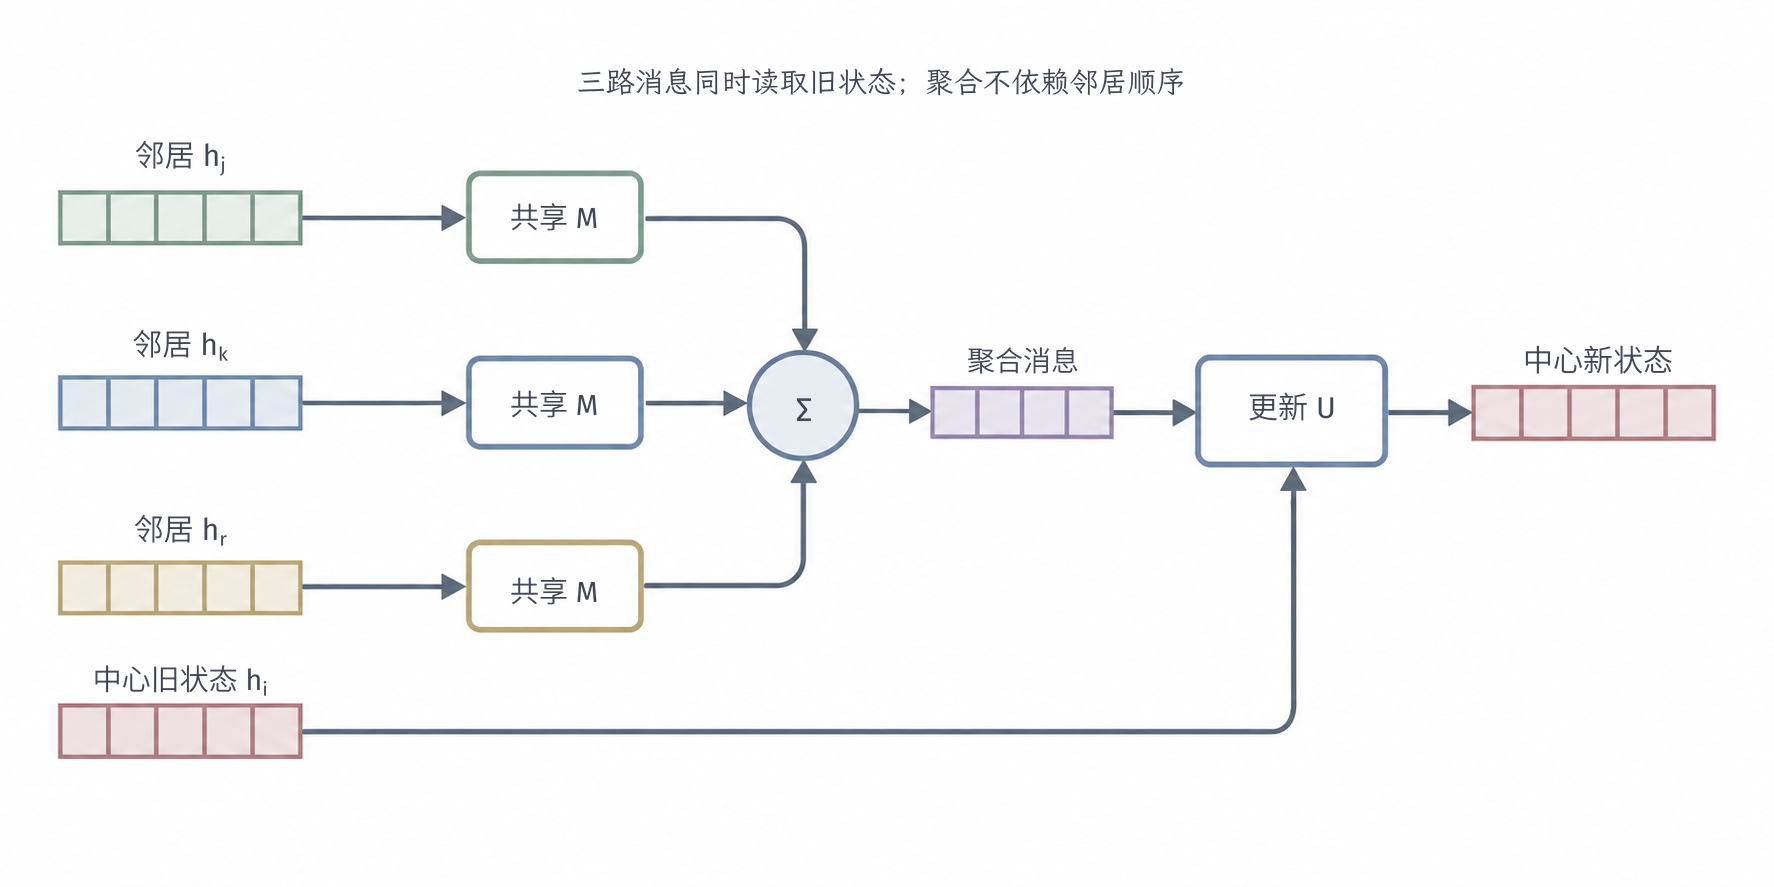
\includegraphics[width=150.199mm]{figures/03-models/02-neural-network-models/generated/gnn-message-passing/figure.png}
  \caption{节点$i$的一轮消息传递。左侧三行邻居表示分别产生消息，经求和聚合后更新节点$i$。下方独立路径把$i$的旧表示送入更新函数。图中省略消息函数对接收节点和边属性的额外输入，所有节点使用相同的消息与更新规则。}
  \label{fig:gnn-message-passing}
\end{figure*}

在同一轮内，$M^{(l)}$和$U^{(l)}$的参数在所有节点与边上共享。因此，增加节点会增加计算量，却不必增加参数量。若邻域聚合不依赖枚举次序，输入编码和节点更新也使用共享函数，就可按轮归纳证明式\eqref{eq:gnn-permutation}：重编号只重排消息的接收位置，聚合结果跟着重排，更新后的表示也跟着重排。随机邻居采样还要求采样规则与编号无关；不同随机抽样下输出数值未必一致，等变性应针对对应的抽样或输出分布理解。

一轮只能读取直接邻居的旧表示。两轮之后，邻居的表示已经包含它们的邻居，节点因而可以利用两跳以内的信息。\term{图上的感受野}（graph receptive field）就是能够经传播影响当前表示的节点范围；在仅使用一跳邻域、没有全局通路时，$L$轮的范围至多为$L$跳。图~\ref{fig:gnn-propagation}采用同步更新：各节点都读取上一轮快照，再形成下一轮快照。若改为读取刚更新的状态，传播次序和一轮可见范围也会随之改变。

\begin{figure}[htb]
  \centering
  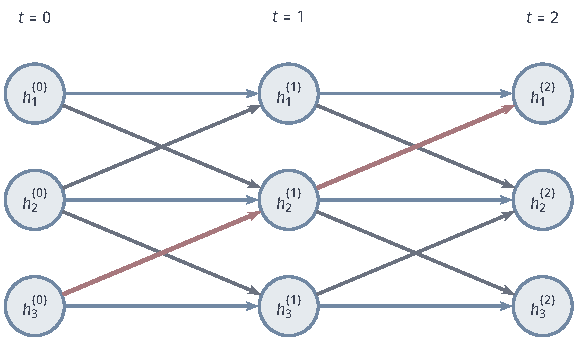
\includegraphics[width=97.794mm]{figures/03-models/02-neural-network-models/tikz/gnn-propagation/figure.pdf}
  \caption{三节点路径上的同步传播。列顶的$t=0,1,2$表示同步快照，横向实线传递自身状态，斜线沿原图的相邻关系传递状态。红色粗线描出节点3经节点2影响节点1的两跳路径；同一列内没有即时传播，因此一次更新不能直接读取两跳之外的新信息。}
  \label{fig:gnn-propagation}
\end{figure}

\begin{example}[两轮邻域平均]
\label{ex:gnn-two-rounds}
取无向路径$1-2-3$，初始标量为$\bm{x}=(1,0,2)^{\top}$。为单独观察传播，暂不使用可学习参数与非线性，令
\[
  h_i^{(l+1)}=\frac{h_i^{(l)}+\sum_{j\in N(i)}h_j^{(l)}}{1+|N(i)|}\text{。}
\]
一轮结果为$(1/2,1,1)^{\top}$，两轮结果为$(3/4,5/6,1)^{\top}$。节点1在第一轮没有读取节点3，第二轮却通过节点2受到节点3的影响。这是人为构造的传播例子，不是训练所得的实验结果。
\end{example}

节点表示形成后，整图预测还需要\term{读出}（readout）：把数量可变的节点表示变成一个图表示。基本形式是
\begin{equation}
  \bm{g}=\rho\!\left(\sum_{i\in V}\phi(\bm{h}_i^{(L)})\right),
  \qquad \widehat{\bm{y}}=g_{\mathrm{out}}(\bm{g})\text{，}
  \label{eq:gnn-readout}
\end{equation}
其中$\phi$是共享的节点变换，$\rho$是聚合后的变换。求和不因节点重排而改变，所以它把节点等变表示转为整图不变表示。平均会消去部分规模信息，最大值强调是否出现某类特征；若目标随对象数量累积，求和更符合这一结构假设，但仍需验证目标是否具有相应可加性。

只计固定宽度$m$下的稠密线性节点变换和线性消息，一轮常可组织为$O(nm^2+em)$：先对节点变换，再沿边聚合。若每条边都单独通过宽度为$m$的稠密网络，边计算可以达到$O(em^2)$。消息函数的形式和特征宽度共同决定边数的成本系数。保存多轮激活时，训练存储也随节点、边及传播轮次增长；参数共享控制的是参数数目。

\subsection{输出和学习目标}
\label{sec:gnn-output-objectives}

预测对象可以是节点、节点对或整张图。三者可以共享同一个图编码器，但监督位置和样本组织不同。图~\ref{fig:gnn-output-levels}把这三种读出对应起来；损失仍按第~\ref{sec:ffn-output-objectives}节所介绍的输出含义选择。

\begin{figure*}[htb]
  \centering
  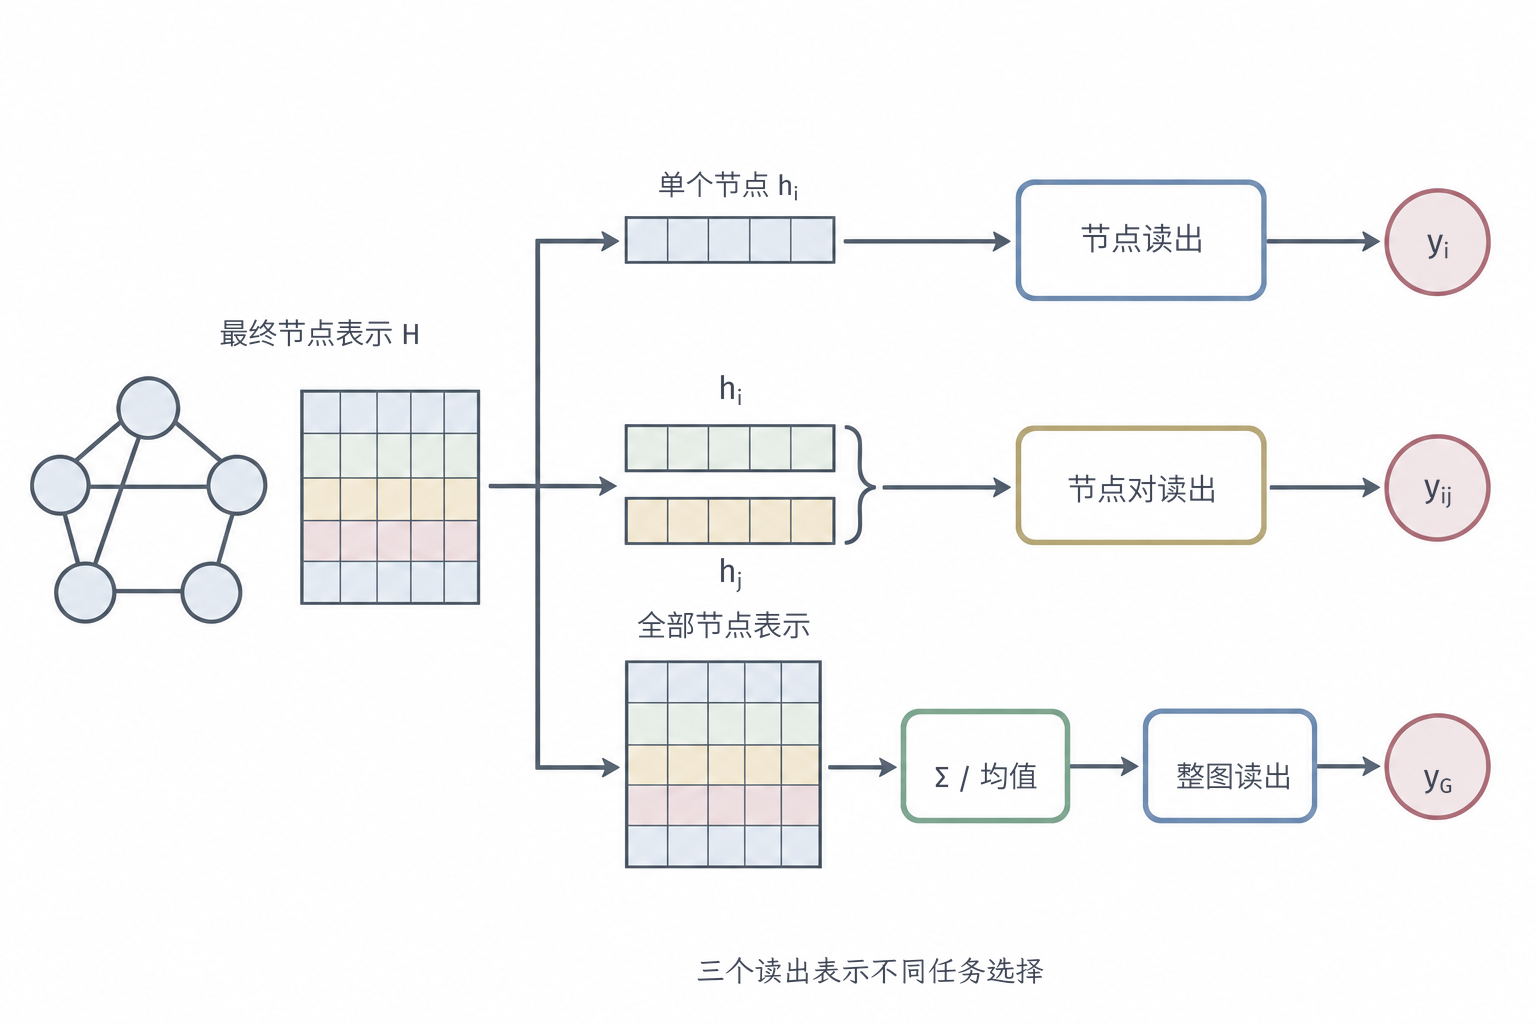
\includegraphics[width=130.048mm]{figures/03-models/02-neural-network-models/generated/gnn-output-levels/figure.png}
  \caption{同一组节点表示的三种任务读出。三个分支分别承载节点、节点对和整图任务，并在相应位置执行读出。节点预测读取一个节点，边或连接预测读取两个端点及可用的关系属性，整图预测先对全部节点作对称聚合；三个分支不要求在同一模型中同时启用。}
  \label{fig:gnn-output-levels}
\end{figure*}

节点分类在每个受监督节点上计算类别概率。设类别数为$C$，标签$y_i\in\{1,\ldots,C\}$，训练标签所在节点集合为$V_{\mathrm{train}}$，则
\begin{equation}
  \begin{aligned}
    \bm{p}_i&=\operatorname{softmax}(\bm{W}_{\mathrm{out}}\bm{h}_i^{(L)}+\bm{b}_{\mathrm{out}}),\\
    L_{\mathrm{node}}&=-\frac{1}{|V_{\mathrm{train}}|}
      \sum_{i\in V_{\mathrm{train}}}\log p_{i,y_i}\text{。}
  \end{aligned}
  \label{eq:gnn-node-loss}
\end{equation}
$\bm{W}_{\mathrm{out}}\in\mathbb{R}^{C\times m_L}$，$\bm{b}_{\mathrm{out}}\in\mathbb{R}^{C}$。其他节点的可见属性与连接可以按任务设定参加编码，类别标签则放在各自的监督或评估集合中。标签掩码限定哪些节点产生训练损失，输入特征的可见范围由另一个规则确定。

边预测需要同时读取端点。设候选节点对集合为$B$，用成对读出函数计算得分，再变成存在连接的预测概率：
\[
  \begin{aligned}
    s_{i,j}&=g_{\mathrm{pair}}(\bm{h}_i^{(L)},\bm{h}_j^{(L)},\bm{a}_{i,j}),\\
    p_{i,j}&=\operatorname{sigmoid}(s_{i,j})\text{。}
  \end{aligned}
\]
对二值目标$b_{i,j}$可使用
\begin{equation}
  L_{\mathrm{edge}}=-\frac{1}{|B|}\sum_{(i,j)\in B}
    \left[b_{i,j}\log p_{i,j}+(1-b_{i,j})\log(1-p_{i,j})\right]\text{。}
  \label{eq:gnn-edge-loss}
\end{equation}
候选连接尚未被观察到时，可用输入通常只含端点和预测时已知的关系类型，读出据此省略未知边属性。无向连接的评分需要满足$s_{i,j}=s_{j,i}$，例如采用点积；有向连接可以使用一般双线性评分或有序拼接，这类有序评分允许两个方向具有不同得分。

整图预测把第$q$张图的读出$\bm{g}_q$映射为类别或数值，按独立图样本平均损失。回归目标$y_q\in\mathbb{R}$可写为
\begin{equation}
  L_{\mathrm{graph}}=\frac{1}{N}\sum_{q=1}^{N}
    \left(g_{\mathrm{out}}(\bm{g}_q)-y_q\right)^2\text{，}
  \label{eq:gnn-graph-loss}
\end{equation}
其中$N$是训练图数，各图的节点数$n_q$可以不同。按图平均给每张图相同权重；按全部节点平均会改变大图与小图的相对权重，二者对应不同的经验目标。

\subsection{参数学习}
\label{sec:gnn-learning}

\subsubsection{沿消息通路回传梯度}
\label{sec:gnn-message-backprop}

固定$L$轮时，式\eqref{eq:gnn-message-passing}是有限的函数复合。前向沿边$j\to i$读取节点$j$的状态，反向则计算这份状态对节点$i$的预测误差有多大影响，再把相应导数回到$j$。前向读取已经建立这条求导依赖，即使原图没有另设$i\to j$的边，导数仍沿链式法则回到发送者。图中的环已沿传播轮次展开，反向依次处理$l=L-1,\ldots,0$，每次回传都进入更早一轮的状态。

用列向量$\bm{g}_i^{(l)}=\partial L/\partial\bm{h}_i^{(l)}\in\mathbb{R}^{m_l}$记节点状态的总梯度。节点分类的输出头在受监督节点产生初始梯度；整图读出把整图损失回传到参与读出的节点；连接预测的评分头向两个端点回传。没有自身标签的节点也可能因影响其他节点的预测而得到梯度。下面暂设损失只经最终轮状态产生，若中间轮也有输出，须在该轮另加直接损失的导数。

一轮反向计算可以对应前向的三个环节。令消息宽度为$r_l$，聚合宽度为$\overline r_l$，先将$\bm{g}_i^{(l+1)}$经更新函数回到聚合向量，再经聚合回到各条消息：
\begin{equation}
  \begin{aligned}
    \bm{v}_i^{(l)}
      &=\left(\frac{\partial U^{(l)}}
        {\partial\overline{\bm{m}}_i^{(l)}}\right)^{\top}
        \bm{g}_i^{(l+1)},\\
    \bm{\delta}_{i\leftarrow j}^{(l)}
      &=\left(\frac{\partial\operatorname{AGG}^{(l)}}
        {\partial\bm{m}_{i\leftarrow j}^{(l)}}\right)^{\top}
        \bm{v}_i^{(l)}\text{。}
  \end{aligned}
  \label{eq:gnn-message-adjoints}
\end{equation}
这里$\bm{v}_i^{(l)}\in\mathbb{R}^{\overline r_l}$，$\bm{\delta}_{i\leftarrow j}^{(l)}\in\mathbb{R}^{r_l}$；两个局部Jacobian矩阵的形状分别为$m_{l+1}\times\overline r_l$和$\overline r_l\times r_l$。所有导数都在前向保存的状态、消息及参数上计算。求和聚合的Jacobian是单位矩阵，所以每条消息收到同一个$\bm{v}_i^{(l)}$；平均聚合再除以邻居数；逐坐标最大值把导数送到被选中的位置，平局处需约定次梯度或记录规则。内容相关权重也依赖状态，求导时其变化与值向量的变化共同进入梯度。

消息函数的两个状态输入会产生不同贡献。记$\bm{J}_{1,i,j}^{(l)}$、$\bm{J}_{2,i,j}^{(l)}\in\mathbb{R}^{r_l\times m_l}$分别为$M^{(l)}$关于接收端状态和发送端状态的Jacobian。节点$j$的总梯度为
\begin{equation}
  \begin{aligned}
    \bm{g}_j^{(l)}
      &=\left(\frac{\partial U^{(l)}}
        {\partial\bm{h}_j^{(l)}}\right)^{\top}
        \bm{g}_j^{(l+1)}\\
      &\quad+\sum_{i:\,j\in N(i)}
        (\bm{J}_{2,i,j}^{(l)})^{\top}
        \bm{\delta}_{i\leftarrow j}^{(l)}\\
      &\quad+\sum_{k\in N(j)}
        (\bm{J}_{1,j,k}^{(l)})^{\top}
        \bm{\delta}_{j\leftarrow k}^{(l)}\text{。}
  \end{aligned}
  \label{eq:gnn-node-state-gradient}
\end{equation}
第一项经过$j$自身的更新分支，局部偏导把聚合输入暂视为固定；第二项汇总$j$向其他节点发送的消息，正是从各接收节点回到$j$的梯度；第三项来自$j$作为接收端参与消息计算的影响。若消息只依赖发送端，第三项为零。自环使同一状态同时充当两个输入，两个局部贡献都要计入；跨层连接也按其实际计算路径另行累加。

图~\ref{fig:gnn-backpropagation}展示第二项的汇合。一个节点被多个接收节点读取时，每条读取路径都有一份导数，节点的总梯度是这些贡献的和。自动微分系统在计算图上完成这种累积；分布式实现若把相关计算放在不同设备上，则需要汇总同一状态和共享参数的贡献。
\begin{figure*}[htb]
  \centering
  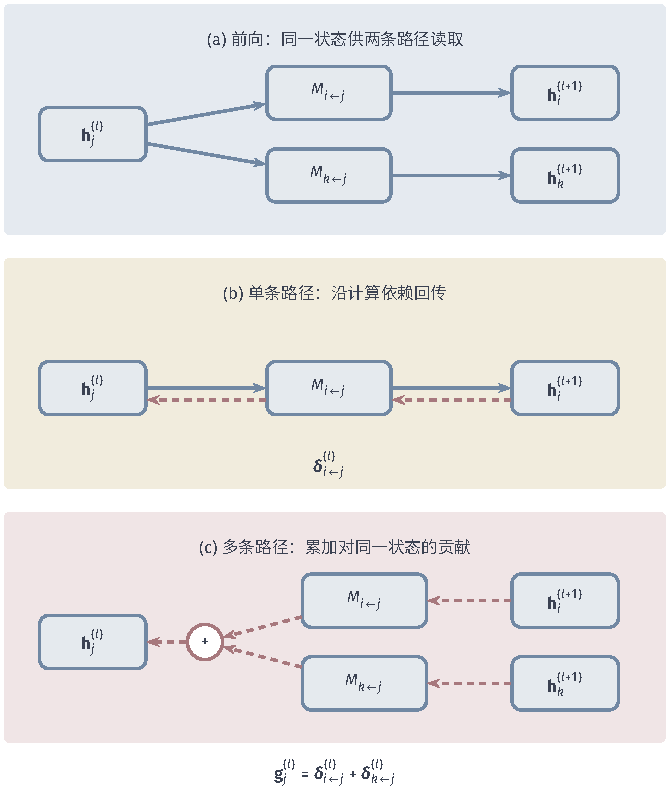
\includegraphics[width=113.404mm]{figures/03-models/02-neural-network-models/tikz/gnn-backpropagation/figure.pdf}
  \caption{一份节点状态的梯度来自多条读取路径。（a）只画前向分叉；（b）单独跟踪一条接收路径的回传；（c）同时回传两条路径，并在$+$处累加为$\bm g_j^{(l)}$。实线表示前向计算，红色虚线表示导数路径。图省略其他邻居的消息、接收节点自身的更新分支和任务输出头；反向依赖由前向读取决定，不要求原图存在反向边。}
  \label{fig:gnn-backpropagation}
\end{figure*}

状态梯度继续传向上一轮，共享参数的梯度则汇集为本次优化器更新的输入。以一层线性消息$\bm{m}_{i\leftarrow j}=\bm{W}\bm{h}_j$为例，$\bm{W}\in\mathbb{R}^{r_l\times m_l}$，接收端回传的消息梯度给发送端贡献$\bm{W}^{\top}\bm{\delta}_{i\leftarrow j}$，并给权重贡献一个外积。因此
\begin{equation}
  \frac{\partial L}{\partial\bm{W}}
    =\sum_{(j\to i)\in E}
      \bm{\delta}_{i\leftarrow j}\bm{h}_j^{\top}\text{。}
  \label{eq:gnn-shared-gradient}
\end{equation}
跨轮共享$\bm{W}$时，还要对轮次求和。节点更新、输入编码及输出头中的共享参数使用同样规则，正则项的导数另加到相应参数。各边、各轮的贡献汇集后，优化器更新这一份共享权重。

\begin{example}[无标签节点怎样得到梯度]
\label{ex:gnn-unlabeled-gradient}
沿用示例~\ref{ex:gnn-two-rounds}的两轮平均，只在节点1设置目标0，取$L=\tfrac12(h_1^{(2)})^2$。此处状态与梯度都是标量，记$g_i^{(l)}=\partial L/\partial h_i^{(l)}$。由$h_1^{(2)}=3/4$，最终轮梯度为$(3/4,0,0)$。节点1的第二轮输出平均了上一轮节点1和2的状态，故
\[
  \bm{g}^{(1)}=(3/8,3/8,0)^{\top},\qquad
  \bm{g}^{(0)}=(5/16,5/16,1/8)^{\top}\text{。}
\]
例如节点3没有标签，却通过节点2影响节点1；它在初始轮收到的梯度为$(3/8)\times(1/3)=1/8$。这里没有可学习的传播参数，例子只核对状态导数。这个导数衡量预测对输入属性的敏感度；当前任务更新的参数范围仍由模型定义。
\end{example}

\subsubsection{训练批次与信息范围}
\label{sec:gnn-training-batches}

\term{全图训练}（full-graph training）在每次前向计算中读取完整训练可见图，再在受监督位置计算损失。单图节点分类可以只抽取一批标签位置，却仍计算全图表示；它与只读取部分结构的训练不同。多个图可以通过块对角邻接矩阵组成一个不连通的大图批次，读出再按图归属分别聚合，使每个分子的节点只形成该分子的表示。

大图上的$L$跳邻域可能迅速膨胀。\term{邻居采样}（neighbor sampling）为本批目标节点逐层选择有限邻居，再在所需计算图上前向和反向。每层最多取$s$个邻居时，未经去重的展开规模可达到$1+s+\cdots+s^L$。采样限制了每个节点的分支数，多层递推仍会展开这些分支。均匀采样的均值可无偏估计一个固定邻域向量的平均，但非线性更新后的预测及其梯度通常不是全图结果的无偏估计，归一化和多层抽样还会进一步改变计算。

\term{子图训练}（subgraph training）抽取一部分节点及相应边，在这张子图中完成多轮传播。它便于多个目标共享计算，但截断边界改变了邻域。若希望保留目标节点完整的$L$跳计算，可以把外围节点作为上下文纳入；使用诱导子图时，边界外消息被省去，度及归一化也按所用近似相应确定。采样误差、边界缺失和标签抽样是不同的变化来源。

数据的可见范围还取决于预测设定。\term{直推学习}（transductive learning）针对训练时已知的一批对象预测未知标签：例如引用图的结构与全文特征可以全部可见，只在部分节点上提供标签。\term{归纳学习}（inductive learning）要求把学到的规则用于此前没有见过的节点或图：训练与预测分别使用当时已知的对象属性和关系。共享消息函数适用于这两种设定：参数随对象复用，是计算结构的性质；新对象上的预测误差，则由相应数据和评估检验。

每次训练更新都应明确可见图、输入特征、监督集合和损失平均方式。对连接预测，还须在编码图中移除待评估的目标边及能直接暴露目标的副本；对动态预测，结构和属性只能来自预测时刻以前。编码图、输入属性与监督目标分别规定可见范围，三者共同确定模型在解答哪个预测问题。

\subsubsection{参数更新与收敛条件}
\label{sec:gnn-optimization-convergence}

反向传播给出当前参数下的导数，优化器才决定怎样改变参数。将全部可学习参数记为$\bm{\theta}\in\mathbb{R}^{p}$，固定数据与可见图，记训练损失加正则项为$J(\bm{\theta})$。一次普通梯度更新为
\begin{equation}
  \bm{\theta}^{(t+1)}=\bm{\theta}^{(t)}
    -\eta_t\widehat{\bm{g}}^{(t)}\text{，}
  \label{eq:gnn-parameter-update}
\end{equation}
$t$是优化器更新次数，与传播轮次$l$不同；$\eta_t>0$是学习率。全目标求导时$\widehat{\bm{g}}^{(t)}=\nabla J(\bm{\theta}^{(t)})$，抽批次时则是相应计算得到的梯度估计。同一次更新的前向和反向使用同一份参数。旧梯度累积按训练规则清除或保留，本批贡献再求和或按约定平均，随后进入优化器。

网络的多层复合、消息函数和输出头通常使$J$非凸。训练进展可以由损失值、梯度尺度或参数变化测量；达到驻点与找到全局最小值又有不同的条件。共享参数与归一化会改变目标及传播尺度，求解保证仍需由完整优化问题建立。

一个有条件的结果说明梯度法为什么可能稳定降低目标。假定$J$有下界$J_{\inf}$，且梯度是$\beta$-Lipschitz的，即$\lVert\nabla J(\bm{u})-\nabla J(\bm{v})\rVert_2\leq\beta\lVert\bm{u}-\bm{v}\rVert_2$，其中$\beta>0$。沿连接两参数的线段积分梯度，可得
\[
  J(\bm{u})\leq J(\bm{v})+
  \langle\nabla J(\bm{v}),\bm{u}-\bm{v}\rangle
  +\frac{\beta}{2}\lVert\bm{u}-\bm{v}\rVert_2^2\text{。}
\]
若使用完整梯度与固定学习率$0<\eta\leq1/\beta$，代入式\eqref{eq:gnn-parameter-update}即得到
\begin{equation}
  \begin{aligned}
    J(\bm{\theta}^{(t+1)})
      &\leq J(\bm{\theta}^{(t)})
        -\frac{\eta}{2}\lVert\nabla J(\bm{\theta}^{(t)})\rVert_2^2,\\
    \min_{0\leq t<T}\lVert\nabla J(\bm{\theta}^{(t)})\rVert_2^2
      &\leq\frac{2[J(\bm{\theta}^{(0)})-J_{\inf}]}{\eta T}\text{。}
  \end{aligned}
  \label{eq:gnn-gradient-descent-bound}
\end{equation}
第二行由第一行对$T$次更新求和得到，$T$是优化步数。它控制前若干次更新中最小的梯度范数平方；在这些假设下，各迭代点的梯度范数也趋于零。参数序列是否有极限、驻点是否全局最优，还需进一步条件。ReLU与最大聚合具有不可微位置，实际目标的有限平滑常数$\beta$也需要在所分析区域建立，光滑结论的适用范围由此确定。

抽样梯度还增加了波动。若它在给定参数下无偏、方差有统一上界，并满足相应光滑性及下界条件，递减学习率可以控制梯度噪声。经典条件包括$\sum_t\eta_t=\infty$和$\sum_t\eta_t^2<\infty$，能保证按学习率加权的期望梯度平方范数平均值趋于零。这个指标描述迭代过程的加权平均，参数极限与全局最优另需条件。固定非零学习率通常只能保证平均梯度大小受噪声项控制，单步损失不必持续下降。Bottou等的分析明确区分了这两种情形\scite{bottou2018optimization} 在固定编码图上，均匀抽取标签位置并按目标正确缩放，可以保持完整标签平均损失的无偏梯度；邻居采样经过多层非线性却未必如此。标签抽样和邻域抽样可能对应不同梯度对象，收敛分析随实际目标和更新规则确定；自适应优化器也需要对应的条件。

实际停止可结合最大步数、在固定评估计算上的训练损失与梯度范数，以及验证指标的早停。传播深度、初始化、度归一化、残差与门控会影响链式Jacobian的尺度，从而影响梯度过小或过大的程度；学习率和优化器也须与该尺度匹配。可以据实际梯度和目标变化检验这些设计对训练条件的影响。固定参数下的状态迭代是否收敛则是另一问题，第~\ref{sec:gnn-state-convergence}节讨论其充分条件；新对象上的误差则由匹配预测设定的数据另行检验。

\section{卷积图神经网络}
\label{sec:gnn-convolutional}

第~\ref{sec:cnn-convolution-definition}节的离散卷积在每个位置使用同一组核系数。一维有限核可写为$y_i=\sum_{r=-K}^{K}w_r x_{i-r}$：位置$i$改变时，系数$w_r$仍对应同一个相对偏移。图也需要共享关系上的计算，却通常没有统一的相对坐标。不同节点的邻居数不同，邻居没有自然次序，也没有一个可在整张图上反复移动的固定窗口。相对偏移$i-r$在图上需要由关系另行定义，节点编号的数值差只反映保存方式。

\term{图卷积}（graph convolution）把规则网格上的共享滤波推广到图信号，即节点上的数值或特征。这个推广有两个互补入口。谱域保留经典卷积定理的形式：先把信号分解成模式，再对各模式的系数乘以滤波响应。空域保留共享局部组合的形式：沿图的邻域，用同一个消息规则计算贡献，再作不依赖邻居次序的聚合。一般图缺少网格上的统一平移；“卷积”因此以图关系上的算子定义，再由该算子决定传播和计算。

一个线性图滤波器可以把两种入口联系起来。令$\bm{Q}\in\mathbb{R}^{n\times n}$是给定的局部传播矩阵，非对角非零元只位于相邻节点间；邻接矩阵就是一个选择。对$\bm{H}\in\mathbb{R}^{n\times d_{\mathrm{in}}}$，可定义
\begin{equation}
  \bm{Z}=\sum_{k=0}^{K}\bm{Q}^{k}\bm{H}\bm{W}_k,
  \qquad \bm{W}_k\in\mathbb{R}^{d_{\mathrm{in}}\times d_{\mathrm{out}}}\text{。}
  \label{eq:gnn-polynomial-convolution}
\end{equation}
其中$\bm{Q}^0=\bm{I}_n$，$\bm{Z}\in\mathbb{R}^{n\times d_{\mathrm{out}}}$；$k=0$处理自身，$k\geq1$组织至多$k$跳内经传播到达的信息。$\bm{W}_k$在所有节点共享，并不为每条具体路径另设参数。计算时递推$\bm{H}_0=\bm{H}$、$\bm{H}_k=\bm{Q}\bm{H}_{k-1}$，累加$\bm{H}_k\bm{W}_k$，无需显式形成通常更稠密的$\bm{Q}^k$。非线性激活再作用于$\bm{Z}$，多层这样的计算构成网络。

式\eqref{eq:gnn-polynomial-convolution}如何包含普通卷积，可以在周期的一维有向网格上看清。取移位矩阵$\bm{T}$，满足$(\bm{T}\bm{x})_i=x_{i-1}$，下标按周期返回；则单通道有限核的循环卷积是$\sum_{r=-K}^{K}w_r\bm{T}^{r}\bm{x}$。不同偏移对应重复移位或反向移位。一般图改用邻接或拉普拉斯等关系算子组织传播。单个无向对称算子把两方向按同一关系处理；带方向或类型差别的核则需要相应的关系信息及不同的关系算子。

共享还必须服从重编号。若$\bm{Q}'=\bm{P}\bm{Q}\bm{P}^{\top}$、$\bm{H}'=\bm{P}\bm{H}$，则$\bm{Z}'=\bm{P}\bm{Z}$，因为$(\bm{P}\bm{Q}\bm{P}^{\top})^k\bm{P}=\bm{P}\bm{Q}^k$。这使局部组合不依赖节点保存次序。但一般消息传递比线性卷积更广：注意力或非线性边消息可以让权重依赖输入，不必对应某个固定的线性频率响应。下面分别从图信号的模式与邻域计算定义具体算子，再比较两者的联系和适用条件。

\subsection{谱域图神经网络}
\label{sec:gnn-spectral}

\subsubsection{图拉普拉斯与图傅里叶变换}
\label{sec:gnn-graph-fourier}

把每个节点上的标量看作图信号，按节点度归一化后的相邻差异刻画它在关系上的变化。对称非负邻接矩阵对应的图拉普拉斯将这些变化分成模式：低频模式变化较缓，高频模式变化较快。本节学习各模式怎样进入输出（谱变换的数学基础参考\BookSectionRef{sec:signal-analysis-graph-state-kernels}{第一卷“数学准备”的“顶点函数的谱变换”小节}）。

记$d_i=\sum_j\bm A_{i,j}$为节点度，$\bm D=\operatorname{diag}(d_1,\ldots,d_n)$为度矩阵。
节点度差异较大时，常用\term{对称归一化拉普拉斯}（symmetric normalized Laplacian）。
本节为简化推导，假定所有节点$d_i>0$，令
\begin{equation}
  \bm{L}=\bm{I}_n-\bm{D}^{-1/2}\bm{A}\bm{D}^{-1/2}
    =\bm{U}\bm{\Lambda}\bm{U}^{\top}\text{。}
  \label{eq:gnn-laplacian-spectrum}
\end{equation}
$\bm{U}\in\mathbb{R}^{n\times n}$的列$\bm{u}_k$是正交特征向量，$\bm{\Lambda}$的对角元素$\lambda_k\in[0,2]$按升序排列。归一化后的能量比较$x_i/\sqrt{d_i}$与$x_j/\sqrt{d_j}$，因此零频模式在每个连通分量内与$\sqrt{d_i}$成比例，未必是常量；不同分量可以具有不同的比例系数。图连通时，零特征空间才只有这一个方向。存在孤立节点时须另规定归一化约定，或加自环后再定义相应算子。

在当前归一化拉普拉斯的图傅里叶坐标$\widehat{\bm x}=\bm U^\top\bm x$中，
让频率响应$g_{\bm\theta}(\lambda)$随训练参数改变，得到可学习的谱滤波：
\begin{equation}
  \bm{y}=\bm{U}g_{\bm{\theta}}(\bm{\Lambda})\bm{U}^{\top}\bm{x}
    =g_{\bm{\theta}}(\bm{L})\bm{x}\text{。}
  \label{eq:gnn-spectral-filter}
\end{equation}
图~\ref{fig:gnn-spectral-filter}显示这三步。谱域图卷积沿用傅里叶域逐模式相乘的形式；图的连接决定这些模式，所以滤波的含义由图谱而非普通空间偏移给出。

\begin{figure*}[htb]
  \centering
  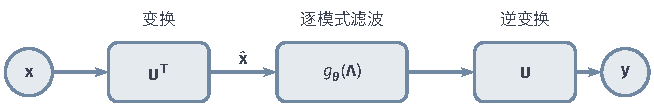
\includegraphics[width=110.793mm]{figures/03-models/02-neural-network-models/tikz/gnn-spectral-filter/figure.pdf}
  \caption{谱滤波的计算路径。节点信号$\bm{x}$经$\bm{U}^{\top}$分解为图傅里叶系数，每个模式由$g_{\bm{\theta}}(\lambda_k)$调整，再经$\bm{U}$还原为节点信号。左、右两端使用同一张图和同一节点顺序；中间向量的下标表示频率模式。}
  \label{fig:gnn-spectral-filter}
\end{figure*}

\begin{example}[三节点路径上的低频模式]
\label{ex:gnn-low-frequency}
沿用路径$1-2-3$，此处不加自环，度为$(1,2,1)$。归一化拉普拉斯的特征值为$0,1,2$，可取
\[
  \bm{u}_1=\tfrac12(1,\sqrt2,1)^{\top},\quad
  \bm{u}_2=\tfrac{1}{\sqrt2}(1,0,-1)^{\top},\quad
  \bm{u}_3=\tfrac12(1,-\sqrt2,1)^{\top}\text{。}
\]
输入$\bm{x}=(1,0,2)^{\top}$的三个系数为$3/2,-1/\sqrt2,3/2$。若只保留零频模式，输出为$(3/4,3\sqrt2/4,3/4)^{\top}$。中间节点的数值较大，恰是度归一化后的平滑，而不是普通算术平均。
\end{example}

\subsubsection{Spectral CNN：直接学习频率响应}
\label{sec:gnn-spectral-cnn}

Bruna等的Spectral CNN把谱滤波放入多通道网络。对输入通道$a$与输出通道$b$，可以学习一个对角滤波器$\bm{\Theta}_{a,b}$，用$\bm{U}\bm{\Theta}_{a,b}\bm{U}^{\top}$变换对应信号，再累加通道并使用非线性。完整谱上的自由响应需要每通道对$n$个参数；原工作还用少量样条系数插值得到平滑响应，减少参数自由度\scite{bruna2014spectral}

固定图与傅里叶基时，前向计算是矩阵乘法，滤波参数可按链式法则求导。例如单通道$\bm{y}=\bm{U}\operatorname{diag}(\bm{\theta})\widehat{\bm{x}}$，上游梯度为$\bm{v}=\partial L/\partial\bm{y}$，则$\partial L/\partial\theta_k=(\bm{U}^{\top}\bm{v})_k\widehat x_k$。通道与样本之间共享参数时，对相应贡献求和即可。

直接使用稠密$\bm{U}$需要$O(n^2)$的单信号变换和存储，完整稠密特征分解的常规代价为$O(n^3)$。只保留部分特征向量可以改变代价，但也限制了可用模式。自由频率响应还可能对应全图稠密算子，读取范围要由实际响应检验；有限跳数局部性需要另加结构。

对新图，特征值与特征向量都会变化，按旧图谱索引学习的自由系数没有自然的一一对应。特征向量的符号在$\bm{U}\bm{\Theta}\bm{U}^{\top}$中相消，但重特征值对应的子空间还可以旋转；若该子空间内使用不同自由系数，算子就依赖具体基的选择。由同一个标量函数$g(\lambda)$定义响应，能够消除这种基选择歧义；跨图迁移的预测效果仍需另行验证。

\subsubsection{ChebNet：用多项式实现局部滤波}
\label{sec:gnn-chebnet}

若滤波器能够直接写成$\bm{L}$的多项式，就可以绕开显式傅里叶基。ChebNet用\term{切比雪夫多项式}（Chebyshev polynomial）参数化响应。设$\lambda_*>0$是拉普拉斯谱的上界，令$\widetilde{\bm{L}}=2\bm{L}/\lambda_*-\bm{I}_n$，把谱放到$[-1,1]$；归一化拉普拉斯可取$\lambda_*=2$。约定$K$为最高次数，则
\begin{equation}
  g_{\bm{\theta}}(\bm{L})\bm{x}
    =\sum_{k=0}^{K}\theta_k T_k(\widetilde{\bm{L}})\bm{x}\text{，}
  \label{eq:gnn-chebyshev-filter}
\end{equation}
其中$T_0(z)=1$、$T_1(z)=z$、$T_k(z)=2zT_{k-1}(z)-T_{k-2}(z)$。有些文献用$K$表示项数，此时最高次数为$K-1$，阅读时须核对约定\scite{defferrard2016chebnet}

令$\bm{z}_k=T_k(\widetilde{\bm{L}})\bm{x}$，即可用$\bm{z}_0=\bm{x}$、$\bm{z}_1=\widetilde{\bm{L}}\bm{x}$以及$\bm{z}_k=2\widetilde{\bm{L}}\bm{z}_{k-1}-\bm{z}_{k-2}$递推。整个过程只需要稀疏矩阵乘向量；单通道的$K\geq1$阶计算量为$O(K(n+e))$，无需构造$\bm{U}$。反向传播也经过这些稀疏乘法，系数梯度为$\bm{v}^{\top}\bm{z}_k$。

多项式为何局部，可以从矩阵乘法看出。$\bm{L}$的非对角非零元只连接相邻节点，一次相乘至多走一条边；$\bm{L}^k$至多连接$k$跳以内。故式\eqref{eq:gnn-chebyshev-filter}在一层中读取至多$K$跳邻域。多通道形式为$\bm{Y}=\sum_{k=0}^{K}T_k(\widetilde{\bm{L}})\bm{X}\bm{\Theta}_k$，$\bm{\Theta}_k\in\mathbb{R}^{d_{\mathrm{in}}\times d_{\mathrm{out}}}$，参数量为$(K+1)d_{\mathrm{in}}d_{\mathrm{out}}$，不随$n$增加。

这些系数描述同一个多项式，所以可以在另一张图上重新构造拉普拉斯并使用它们，无需对齐特征向量。频率分布与任务关系随图改变，预测质量也需在新图上检验。若使用的谱上界过小，使缩放后的特征值落到$[-1,1]$以外，高次多项式还可能迅速放大误差。

\subsection{空域图神经网络}
\label{sec:gnn-spatial}

空域方法直接回答节点怎样读取邻居。下面四种模型分别突出固定归一化、采样与分开组合、内容相关加权，以及邻域多重集合的区分能力。它们共享输出与反向传播的基础，主要差别落在聚合和更新上。

\subsubsection{GCN：归一化的邻域传播}
\label{sec:gnn-gcn}

\term{图卷积网络}（graph convolutional network, GCN）在本节特指Kipf与Welling提出的层形式。加入自环$\widetilde{\bm{A}}=\bm{A}+\bm{I}_n$，令$\widetilde d_i=\sum_j\widetilde{\bm{A}}_{i,j}$，定义传播矩阵
\begin{equation}
  \bm{S}=\widetilde{\bm{D}}^{-1/2}\widetilde{\bm{A}}\widetilde{\bm{D}}^{-1/2},
  \qquad
  \bm{H}^{(l+1)}=\sigma\!\left(\bm{S}\bm{H}^{(l)}\bm{W}^{(l)}\right)\text{。}
  \label{eq:gnn-gcn-layer}
\end{equation}
$\bm{H}^{(l)}\in\mathbb{R}^{n\times m_l}$按行存放状态，$\bm{H}^{(0)}=\bm{X}$；$\bm{W}^{(l)}\in\mathbb{R}^{m_l\times m_{l+1}}$变换特征通道，$\sigma$逐坐标作用。采用行存放的矩阵形式时，节点列向量的变换对应$(\bm{W}^{(l)})^{\top}\bm{h}_i^{(l)}$。原始层式省略偏置，增加共享偏置不会改变置换等变性。

从节点$j$到$i$的消息系数为$\widetilde{\bm{A}}_{i,j}/\sqrt{\widetilde d_i\widetilde d_j}$，同时计入边权以及接收端与发送端的度。边权为1时，才简化为$1/\sqrt{\widetilde d_i\widetilde d_j}$。这个组合按两端度归一化；$\bm{S}$的行和未必等于1，数值因此不同于算术平均。沿用三节点无权路径与输入$(1,0,2)^{\top}$，取单位特征变换和恒等激活，得到
\begin{equation}
  \bm{S}=\begin{pmatrix}
    1/2&1/\sqrt6&0\\
    1/\sqrt6&1/3&1/\sqrt6\\
    0&1/\sqrt6&1/2
  \end{pmatrix},\qquad
  \bm{S}\bm{x}=\begin{pmatrix}1/2\\3/\sqrt6\\1\end{pmatrix}\text{。}
  \label{eq:gnn-gcn-example}
\end{equation}
这一结果与示例~\ref{ex:gnn-two-rounds}的平均不同，差别来自归一化规则。

它与谱域方法的联系可以直接推导。对不加自环的归一化拉普拉斯，ChebNet取$K=1$及$\lambda_*=2$时，$\widetilde{\bm{L}}=-\bm{D}^{-1/2}\bm{A}\bm{D}^{-1/2}$。再约束$\theta_0=-\theta_1=\theta$，得到$\theta(\bm{I}_n+\bm{D}^{-1/2}\bm{A}\bm{D}^{-1/2})\bm{x}$。GCN进一步以加自环后重新计算度的$\bm{S}$替换括号内算子，限制反复传播的尺度。这一步更换了传播算子及其度归一化；原论文称其为重新归一化技巧\scite{kipf2017gcn}

固定结构时，GCN的梯度也可写清。记$\bm{Z}=\bm{S}\bm{H}\bm{W}$，$\bm{\Delta}=\partial L/\partial\bm{Z}$，则
\begin{equation}
  \frac{\partial L}{\partial\bm{W}}=(\bm{S}\bm{H})^{\top}\bm{\Delta},\qquad
  \frac{\partial L}{\partial\bm{H}}=\bm{S}^{\top}\bm{\Delta}\bm{W}^{\top}\text{。}
  \label{eq:gnn-gcn-backprop}
\end{equation}
激活的导数已并入$\bm{\Delta}$。不学习邻接关系时，$\bm{S}$作为给定算子；学习边权或建图规则时，才需进一步计算结构相关梯度。

标准GCN直接混合相邻节点的变换特征。相邻对象与预测目标相关时，这种共享聚合可以提供有用信息；相邻节点常具有不同标签或关系语义时，混合也可能损失区分所需的特征。共享权重可以接新图重建的传播算子；归纳表现需要按照新图的信息范围和数据检验，原始实验设定只说明其当时的任务。

\subsubsection{GraphSAGE：采样并学习邻域组合}
\label{sec:gnn-graphsage}

在很大的图上，为一批目标节点计算全部邻域代价高；新节点到达后，也希望直接用属性及邻域产生表示。GraphSAGE把采样与聚合纳入这一过程。以平均聚合为例，从$N(i)$中取$S_i^{(l)}$，令
\begin{equation}
  \begin{aligned}
    \bm{u}_i^{(l)}&=\frac{1}{|S_i^{(l)}|}\sum_{j\in S_i^{(l)}}\bm{h}_j^{(l)},\\
    \bm{h}_i^{(l+1)}&=\sigma\!\left(
      \bm{W}^{(l)}[\bm{h}_i^{(l)};\bm{u}_i^{(l)}]+\bm{b}^{(l)}\right)\text{。}
  \end{aligned}
  \label{eq:gnn-graphsage}
\end{equation}
分号表示向量拼接，此处$\bm{W}^{(l)}\in\mathbb{R}^{m_{l+1}\times2m_l}$。自身和邻居先分开，再由不同的权重块组合；原算法还可对输出作$\ell_2$归一化，零向量需要单独处理\scite{hamilton2017graphsage}

聚合器也可对邻居先作共享前馈变换，再取逐坐标最大值。平均保留总体水平，最大池化突出某种响应是否出现。原论文还试验了对随机邻居顺序使用LSTM的聚合器。一次LSTM输出取决于所抽顺序；对称聚合直接消除枚举次序，随机顺序方案则需说明对称化或输出分布的口径。

训练时采样所需邻域，计算节点或关系任务的损失，联合更新聚合器、组合矩阵及输出头。预测新节点时沿相同规则读取可用特征与邻域，不必为它单独学习一个节点编号嵌入。新节点可提供的属性与邻域决定表示的信息来源。只使用旧节点编号时，可迁移属性不足；新节点缺乏特征或邻居时也需要相应初态或补充输入。

\subsubsection{GAT：根据内容调整邻居权重}
\label{sec:gnn-gat}

固定度归一化没有区分“邻居与当前任务是否相关”。\term{图注意力网络}（graph attention network, GAT）用节点特征计算邻居权重，再在图约束的可见范围内加权聚合。对一个注意力头，令$\bm{z}_i=\bm{W}\bm{h}_i$，其中$\bm{W}\in\mathbb{R}^{m'\times m}$，则
\begin{equation}
  \begin{aligned}
    e_{i,j}&=\operatorname{LeakyReLU}
      \!\left(\bm{a}^{\top}[\bm{z}_i;\bm{z}_j]\right),\\
    \alpha_{i,j}&=\frac{\exp(e_{i,j})}
      {\sum_{k\in N(i)\cup\{i\}}\exp(e_{i,k})},\\
    \bm{h}'_i&=\sigma\!\left(\sum_{j\in N(i)\cup\{i\}}
      \alpha_{i,j}\bm{z}_j\right)\text{。}
  \end{aligned}
  \label{eq:gnn-gat}
\end{equation}
$\bm{a}\in\mathbb{R}^{2m'}$是共享评分参数；$e_{i,j}$是标量得分，与本章的边数$e$不同。Softmax只在节点$i$的可见邻域内归一化，所有节点使用同一评分函数，所以邻居重排只重排对应权重\scite{velickovic2018gat}

多头注意力分别学习变换和评分，在隐藏层拼接结果，或在输出层取平均。训练时梯度同时通过值向量和权重；若把权重当作常量，就漏掉了评分函数对损失的影响。固定每头宽度时，增加头数还会增加总宽度和参数量，相同宽度预算下的比较需相应分配各头维度。

与前章的循环注意力一样，GAT把“计算权重”和“读取信息”分开；区别是可见位置由图的邻接关系约束。原始GAT的评分使用线性拼接，若将$\bm{a}$拆成两部分，得分是单调激活作用于一个接收端项与一个发送端项之和。因此，在固定候选邻居特征下，邻居排序不能仅靠改变接收端特征任意翻转。这说明原始评分虽随内容产生权重，候选排序仍受到该加性结构的限制。

注意力调整可见邻居之间的相对影响，单轮读取范围仍由图限定。归一化权重描述一次聚合中的数值比例，预测作用还取决于表示内容、评分变化及后续计算；解释或因果结论需要另外的证据。

\subsubsection{GIN：保留邻域多重集合的差别}
\label{sec:gnn-gin}

聚合不仅影响尺度，还决定哪些输入差异会在计算中消失。例如邻域$\{\!\{1,1\}\!\}$与$\{\!\{1,1,1\}\!\}$具有相同平均和最大值，但个数不同。另一个例子$\{\!\{0,2\}\!\}$与$\{\!\{1,1\}\!\}$连原始数值的和也相同；先将这些标量映成能保留所需差异的特征，再求和，才可能区分它们。图~\ref{fig:gnn-aggregation}展示第一种信息损失。

\begin{figure*}[htb]
  \centering
  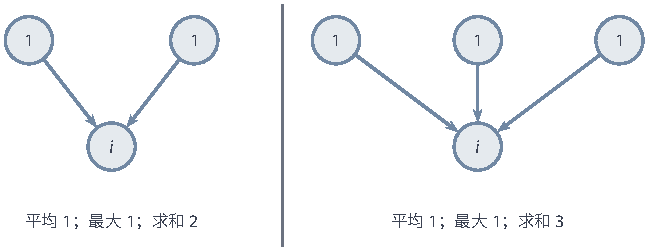
\includegraphics[width=109.792mm]{figures/03-models/02-neural-network-models/tikz/gnn-aggregation/figure.pdf}
  \caption{聚合如何保留或丢掉重复次数。两个邻域分别含两个和三个数值为1的邻居。平均与最大值都产生1，求和分别产生2和3。图只比较固定标量消息；求和本身也不能区分所有不同多重集合，还需要合适的特征映射。}
  \label{fig:gnn-aggregation}
\end{figure*}

\term{图同构网络}（graph isomorphism network, GIN）使用求和聚合与前馈更新：
\begin{equation}
  \bm{h}_i^{(l+1)}=\operatorname{MLP}^{(l)}\!\left(
    (1+\epsilon^{(l)})\bm{h}_i^{(l)}
      +\sum_{j\in N(i)}\bm{h}_j^{(l)}\right)\text{，}
  \label{eq:gnn-gin}
\end{equation}
$\epsilon^{(l)}$可以固定或学习，用于区分中心节点与邻居的贡献。参数通过任务损失反向传播；整图读出还可拼接各层节点求和，保留不同传播范围的信息\scite{xu2019gin}

比较两张图时，若存在保持连接关系及给定属性的节点重编号，使两图相互对应，就称它们\term{同构}（isomorphic）。GIN的区分能力通过下面的标记更新检验作比较。衡量其区分能力的一种参照是\term{一维Weisfeiler--Leman检验}（1-dimensional Weisfeiler--Leman test, 1-WL）：从与节点属性一致的初始标记出发，反复用“节点旧标记及邻居标记的多重集合”产生新标记。所比较的图必须使用同一套无冲突标记规则，相同的输入组合得到相同标记，不同组合得到不同标记。每轮比较两图全部节点标记组成的多重集合；只要有一轮不同，就可判为非同构，始终相同时，检验仍留下未判定的图对。

对于只使用节点状态、对称邻域聚合且不引入额外区分信息的消息传递网络，1-WL无法区分的图也不能靠这些更新与节点多重集合读出区分：同标记节点具有同样的邻域标记多重集合，共享计算遂逐轮产生同样的状态。

在可数特征域、邻域大小有界，以及聚合、更新和读出满足相应单射性条件时，求和特征映射可以达到1-WL的区分能力。\term{单射}（injective）表示不同输入不会被映成同一个结果。有限宽度和训练得到的映射，需要按实际输入检查前述特征域与单射条件。

1-WL本身也有边界。六节点环与两个互不连接的三角形都具有六个节点，每个节点度为2。若初始节点特征全部相同，这两张图上的节点在每轮都会收到两个相同状态，任何上述消息传递加节点多重集合读出都无法区分它们。共同的两邻居模式随轮次持续重复，单靠更多轮数仍无法区分。子结构信息、更高阶状态或其他任务输入可以改变这类区分条件；由数据学得的预测质量还由训练与泛化分析评价。

\subsection{谱域与空域的联系、区别及选择}
\label{sec:gnn-spectral-spatial-comparison}

谱域与空域的区别主要在于怎样规定算子，而不是计算一定发生在哪一类存储空间。谱域用$g_{\bm{\theta}}(\lambda)$规定不同变化模式的响应，空域用邻居的选择、消息和聚合规定局部组合。若$g_{\bm{\theta}}$是多项式，$\bm{U}g_{\bm{\theta}}(\bm{\Lambda})\bm{U}^{\top}$等于同一多项式作用于$\bm{L}$，便可完全通过节点域稀疏传播计算。ChebNet由谱域设计、按邻域递推实现，GCN也保留了谱域推导。谱域规定响应，节点域稀疏传播实现它；同一模型由此可以同时具有频率与局部邻域解释。

表~\ref{tab:gnn-spectral-spatial}将显式谱实现与多项式实现分开。比较计算量时固定一张稀疏图与单通道线性传播，不计特征通道变换、消息网络及初次特征分解的代价；任意空域消息网络的成本还取决于其具体函数。
\begin{table*}[htb]
  \centering
  \small
  \begin{tabularx}{\linewidth}{@{}p{17mm}XXX@{}}
    \toprule
    比较方面 & 显式谱基滤波 & 多项式谱滤波 & 局部空域聚合\\
    \midrule
    算子定义 & 在图傅里叶模式上规定响应 & 用低阶多项式参数化响应 & 用邻居消息、权重及更新规定组合\\
    实际计算 & $\bm{U}^{\top}$、对角滤波、$\bm{U}$ & 拉普拉斯的稀疏乘法递推 & 沿可见边计算，再按节点聚合\\
    局部范围 & 自由响应通常涉及全图 & $K$次多项式至多读取$K$跳 & 一轮通常读取一跳；可另加长程边\\
    传播成本 & 稠密基下$O(n^2)$ & $O(K(n+e))$ & 一跳简单聚合为$O(n+e)$\\
    跨图使用 & 按旧谱索引的自由参数缺少自然对应 & 共享多项式系数，在新图重建算子 & 共享消息规则，在新图读取邻域\\
    \bottomrule
  \end{tabularx}
  \caption{谱域与空域图卷积的比较。显式谱基滤波表示直接使用完整图傅里叶基的实现；多项式谱滤波同时具有有限邻域解释。跨图使用一行只说明计算规则能否复用，不能据此保证新图上的预测效果。}
  \label{tab:gnn-spectral-spatial}
\end{table*}

在大图、多个大小不同的图或不断变化的图上，直接依赖完整$\bm{U}$有几项实际困难。特征分解与稠密变换占用时间和存储，图结构改变后还需处理新的谱；按某张图谱索引学习的系数无法直接对应另一张图的模式。一般自由响应又不是严格局部的，一批目标节点可能依赖大量其他节点，难以只取少量邻居完成同一计算。这些条件解释了为何直接使用完整特征基的早期实现较少成为大规模局部模型的计算方式。

沿边的空域计算容易与邻居采样及小批次结合，也便于让消息读取边类型、方向和接收端内容。复杂度在稀疏图与固定宽度下可随边数增长，参数不必随节点数增加。这种组织便于局部计算，优化和信息保留还取决于消息、深度和数据。多项式谱滤波也能绕开显式特征分解、共享局部传播；它与自由谱基实现的成本和读取范围分别比较。

完整谱基、多项式滤波和空域聚合提供了不同的计算取舍，选择时应回到所需关系。若关心图信号哪些频率应保留或抑制，谱响应提供了直接的设计和分析对象；若需要不同边类型、内容相关交互或采样邻域，空域消息规则更便于表达这些计算。固定线性滤波、有限邻域与跨图复用可以同时成立；输入相关的非线性消息则未必是单个固定谱滤波器。比较两类网络时，应同时写清算子定义、实际实现、可见范围和数据条件。

谱滤波的后续研究继续改进参数化与计算方式。2022年的ChebNetII通过切比雪夫插值组织可学习的谱响应，改进原有滤波器的参数化\scite{he2022chebnetii} 2026年的L2G-NET研究图傅里叶变换的结构化分解，用子图谱表示及其组合处理局部与全局信息，针对完整谱变换的成本和局部性提出新的计算方式\scite{fernandez2026l2gnet} 这些工作进一步探索了频率响应、局部传播和全局交互之间的联系，各自的收益需要结合任务与数据检验。

\section{循环图神经网络}
\label{sec:gnn-recurrent}

前面的网络可以为每层学习不同的变换。若希望同一套关系推理反复执行，就可以跨传播轮次共享参数。本节始终固定输入图；传播轮次表示算法内部更新次数，现实时间变化另在第~\ref{sec:gnn-dynamic}节处理。

\subsection{网络结构}
\label{sec:gnn-recurrent-structure}

\term{循环图神经网络}（recurrent graph neural network）在同一图上反复更新节点隐状态。将全部状态按节点堆成列向量$\bm{h}^{(t)}\in\mathbb{R}^{nm}$，令参数向量为$\bm{\theta}\in\mathbb{R}^{p}$，可写为
\begin{equation}
  \bm{h}^{(t+1)}=F_{\bm{\theta}}(\bm{h}^{(t)};\mathcal{G},\bm{X}),
  \qquad \widehat{\bm{y}}=g_{\bm{\theta}}(\bm{h}^{(T)})\text{。}
  \label{eq:gnn-recurrent-update}
\end{equation}
$F_{\bm{\theta}}$内部仍包含共享消息、聚合与节点更新；分号后的图与属性在各轮固定。图~\ref{fig:gnn-recurrent}显示同一规则的多次调用，每次调用的状态值不同。跨轮共享还要求相应状态维度兼容。

\begin{figure*}[htb]
  \centering
  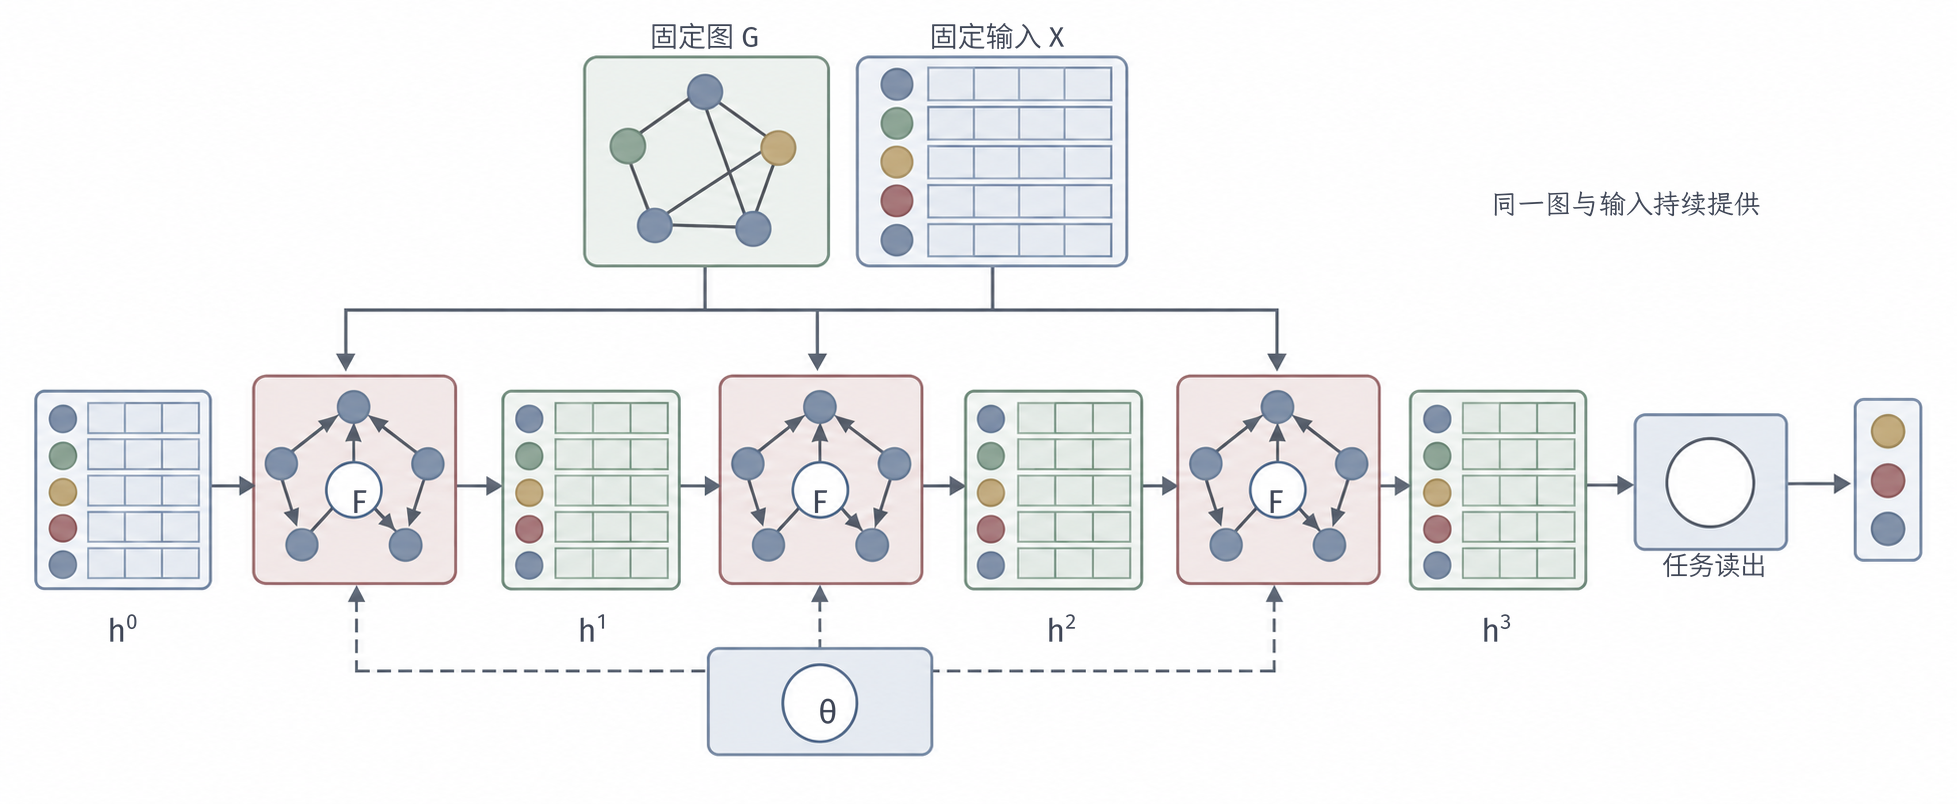
\includegraphics[width=165.693mm]{figures/03-models/02-neural-network-models/generated/gnn-recurrent/figure.png}
  \caption{固定图上的循环更新。左侧表示邻接关系，右侧展开三轮共享更新$F_{\bm{\theta}}$，每个状态向量包含整张图的节点状态。固定图与输入特征在各轮重复供给，状态沿轮次传递，任务读出从最终状态形成预测。轮次是内部计算步，不表示图已经发生三个时间点的变化。}
  \label{fig:gnn-recurrent}
\end{figure*}

共享参数使每轮复用同一规则，执行代价仍累加各轮计算。状态更新和任务监督决定传播内容；若目标是最短路或关系推理，还需检验这些表示与目标规则的对应。有限轮次模型与迭代至稳定的模型分别定义不同的输出。

\subsection{典型模型}
\label{sec:gnn-recurrent-models}

\subsubsection{以不动点为目标的图网络}
\label{sec:gnn-fixed-point-model}

早期GNN把目标状态定义为\term{不动点}（fixed point）：再次使用更新函数后仍不改变的状态，即$\bm{h}^*=F_{\bm{\theta}}(\bm{h}^*;\mathcal{G},\bm{X})$。它通过邻居状态迭代计算这一表示，再读取节点或图输出。为保证状态可确定，模型约束更新对状态具有收缩性；第~\ref{sec:gnn-propagation-theory}节之后的状态收敛分析将给出条件及误差界。

这类模型的参数既影响输出映射，也影响不动点的位置。有限精度计算通常在相邻两轮差小于容差时停止，并设置最大轮数。达到轮数上限时输出当前近似状态，与容差已满足的情况分别记录。所需精度、迭代成本和收缩约束共同决定这一表示怎样求得。

\subsubsection{GGNN：固定轮次的门控传播}
\label{sec:gnn-ggnn}

如果任务只需要执行有限步，可以直接学习这些步骤的结果。\term{门控图神经网络}（gated graph neural network, GGNN）在聚合后用GRU式更新保留或写入状态。令$r(i,j)$表示边的类型与方向，邻域输入为
\begin{equation}
  \bm{a}_i^{(t)}=\sum_{j\in N(i)}\bm{W}_{r(i,j)}\bm{h}_j^{(t-1)}+\bm{b},
  \qquad
  \bm{h}_i^{(t)}=\operatorname{GRU}(\bm{h}_i^{(t-1)},\bm{a}_i^{(t)})\text{。}
  \label{eq:gnn-ggnn}
\end{equation}
这里$\bm{a}_i^{(t)}$是聚合输入向量，与边属性$\bm{a}_{i,j}$通过索引形式区分。原模型分别处理入边与出边并组合相应消息；式\eqref{eq:gnn-ggnn}写出一个统一的关系聚合形式，方向也可编码为不同类型\scite{li2016ggnn}

GRU的门机制沿用第~\ref{sec:rnn-gru}节。若把更新门解释为写入比例，状态可写为$\bm{h}_i^{(t)}=(\bm{1}-\bm{z}_i^{(t)})\odot\bm{h}_i^{(t-1)}+\bm{z}_i^{(t)}\odot\widetilde{\bm{h}}_i^{(t)}$；候选状态同时依赖聚合输入与经重置门处理的旧状态。门为节点提供选择性保留路径，远处证据则仍须沿边经过足够轮次。

GGNN用预先设定的$T$轮展开计算并训练，输出定义为第$T$轮状态，无需把它作为不动点近似。有限展开放宽了早期模型的收缩约束，状态行为由这些实际步骤决定。训练轮数是模型的一部分；预测时增加轮次就改变了所执行的函数，需要相应检验。

\subsection{参数学习}
\label{sec:gnn-recurrent-learning}

有限展开的梯度与随时间反向传播具有相同结构。设局部状态Jacobian矩阵$\bm{J}^{(t)}=\partial\bm{h}^{(t+1)}/\partial\bm{h}^{(t)}$，$\bm{\delta}^{(t)}$为第$t$轮状态的总梯度。若损失只读取末状态，则$\bm{\delta}^{(t)}=(\bm{J}^{(t)})^{\top}\bm{\delta}^{(t+1)}$；中间轮存在直接监督时，另加对应梯度。共享更新参数的梯度为
\begin{equation}
  \nabla_{\bm{\theta}}L
    =\left.\nabla_{\bm{\theta}}L\right|_{\mathrm{direct}}
      +\sum_{t=0}^{T-1}(\bm{B}^{(t)})^{\top}\bm{\delta}^{(t+1)}\text{，}
  \label{eq:gnn-recurrent-gradient}
\end{equation}
其中$\bm{B}^{(t)}=\partial F_{\bm{\theta}}(\bm{h}^{(t)};\mathcal{G},\bm{X})/\partial\bm{\theta}$固定当前输入状态求偏导。直接项包含读出参数等依赖；初态若依赖参数，还需计入初态梯度。截断展开会遗漏更早的间接贡献，降低存储与计算的同时改变所用梯度。

不动点模型还可用\term{隐式微分}（implicit differentiation）：对定义状态的方程求导，而不保存全部前向迭代。假设更新在不动点附近可微，令$\bm{J}_*=\partial F/\partial\bm{h}$、$\bm{B}_*=\partial F/\partial\bm{\theta}$在$\bm{h}^*$处取值。若$\bm{I}-\bm{J}_*$可逆，则
\begin{equation}
  (\bm{I}-\bm{J}_*)\frac{\partial\bm{h}^*}{\partial\bm{\theta}}
    =\bm{B}_*\text{。}
  \label{eq:gnn-implicit-state-gradient}
\end{equation}
这个等式来自对$\bm{h}^*=F_{\bm{\theta}}(\bm{h}^*)$两侧求导，并把状态导数项移到左侧。

实际需要的是标量损失的梯度。记$\bm{v}=\partial L/\partial\bm{h}^*$为列向量，解线性方程
\begin{equation}
  (\bm{I}-\bm{J}_*^{\top})\bm{u}=\bm{v},\qquad
  \nabla_{\bm{\theta}}L
    =\left.\nabla_{\bm{\theta}}L\right|_{\mathrm{direct}}+\bm{B}_*^{\top}\bm{u}\text{。}
  \label{eq:gnn-implicit-loss-gradient}
\end{equation}
无需显式求逆。若相应范数下$\lVert\bm{J}_*\rVert<1$，可用$\bm{u}^{(k+1)}=\bm{v}+\bm{J}_*^{\top}\bm{u}^{(k)}$迭代；Jacobian转置与向量的乘积由自动微分计算。前向状态与后向线性求解都有容差，两者都会影响最终梯度的精度。

对只迭代到近似状态的模型，有限展开给出实际执行步骤的梯度，隐式方法近似理想不动点目标的梯度，二者在尚未充分收敛时未必相同。停止条件、最大轮数和状态收缩速度因而既影响前向代价，也影响参数学习。

\section{图神经网络的扩展}
\label{sec:gnn-extensions}

普通图上的一套聚合规则把每条边都当成成对的信息通路。现实关系还可能具有不同语义，随时间变化，涉及多个参与者，或依赖空间位置。扩展模型需要保留这些输入差异，并把它们放到相应的消息、状态和对称性约束中。

\subsection{多关系与异构图}
\label{sec:gnn-relational}

引用和撰写让论文与邻居发生不同联系；分别记录关系类型，可以让消息保留这种语义差别。\term{多关系图}（multi-relational graph）允许边具有不同关系类型；\term{异构图}（heterogeneous graph）还允许不同节点类型具有不同的属性和角色。节点类型与边类型是两个分类维度，可以单独指定，也可以同时存在。

设关系类型集合为$R$，$N_r(i)$是通过类型$r$向$i$发送消息的邻居。\term{关系图卷积网络}（relational graph convolutional network, R-GCN）为不同关系使用不同变换：
\begin{equation}
  \bm{h}_i^{(l+1)}=\sigma\!\left(
    \bm{W}_0^{(l)}\bm{h}_i^{(l)}+
    \sum_{r\in R}\sum_{j\in N_r(i)}
      \frac{1}{c_{i,r}}\bm{W}_r^{(l)}\bm{h}_j^{(l)}\right)\text{。}
  \label{eq:gnn-rgcn}
\end{equation}
$c_{i,r}>0$是归一化系数，可在非空邻域取$|N_r(i)|$；空邻域的求和直接为零。$\bm{W}_0^{(l)}$负责自身状态，$\bm{W}_r^{(l)}$负责关系$r$。有向关系可增加单独的逆关系类型，使两个方向使用不同参数\scite{schlichtkrull2018rgcn}

关系数很大时，每种关系独立学习一个稠密矩阵会增加参数与数据需求。可以用基分解$\bm{W}_r=\sum_{b=1}^{B}a_{r,b}\bm{V}_b$，让各关系共享$B$个基础矩阵，只学习不同系数。固定输入输出宽度$m$时，参数量由$|R|m^2$改为$Bm^2+|R|B$，代价是关系变换被限制在同一矩阵子空间。

不同节点类型的原始特征维度可能不同，可以先用类型相关的输入映射投到公共空间，再按关系传递。聚合还可先在每种关系内部组合，再学习关系间权重。置换等变性在重编号后仍成立，但类型也须跟着节点与边重排。作者和论文的属性角色保持各自含义，重编号只改变保存它们的位置。

图~\ref{fig:gnn-typed-relations}用作者与论文两类节点说明这种分工。类型映射先对齐特征空间，关系变换与归一化随后保留“撰写”和“引用”的区别，自身状态仍有独立路径。

\begin{figure*}[htbp]
  \centering
  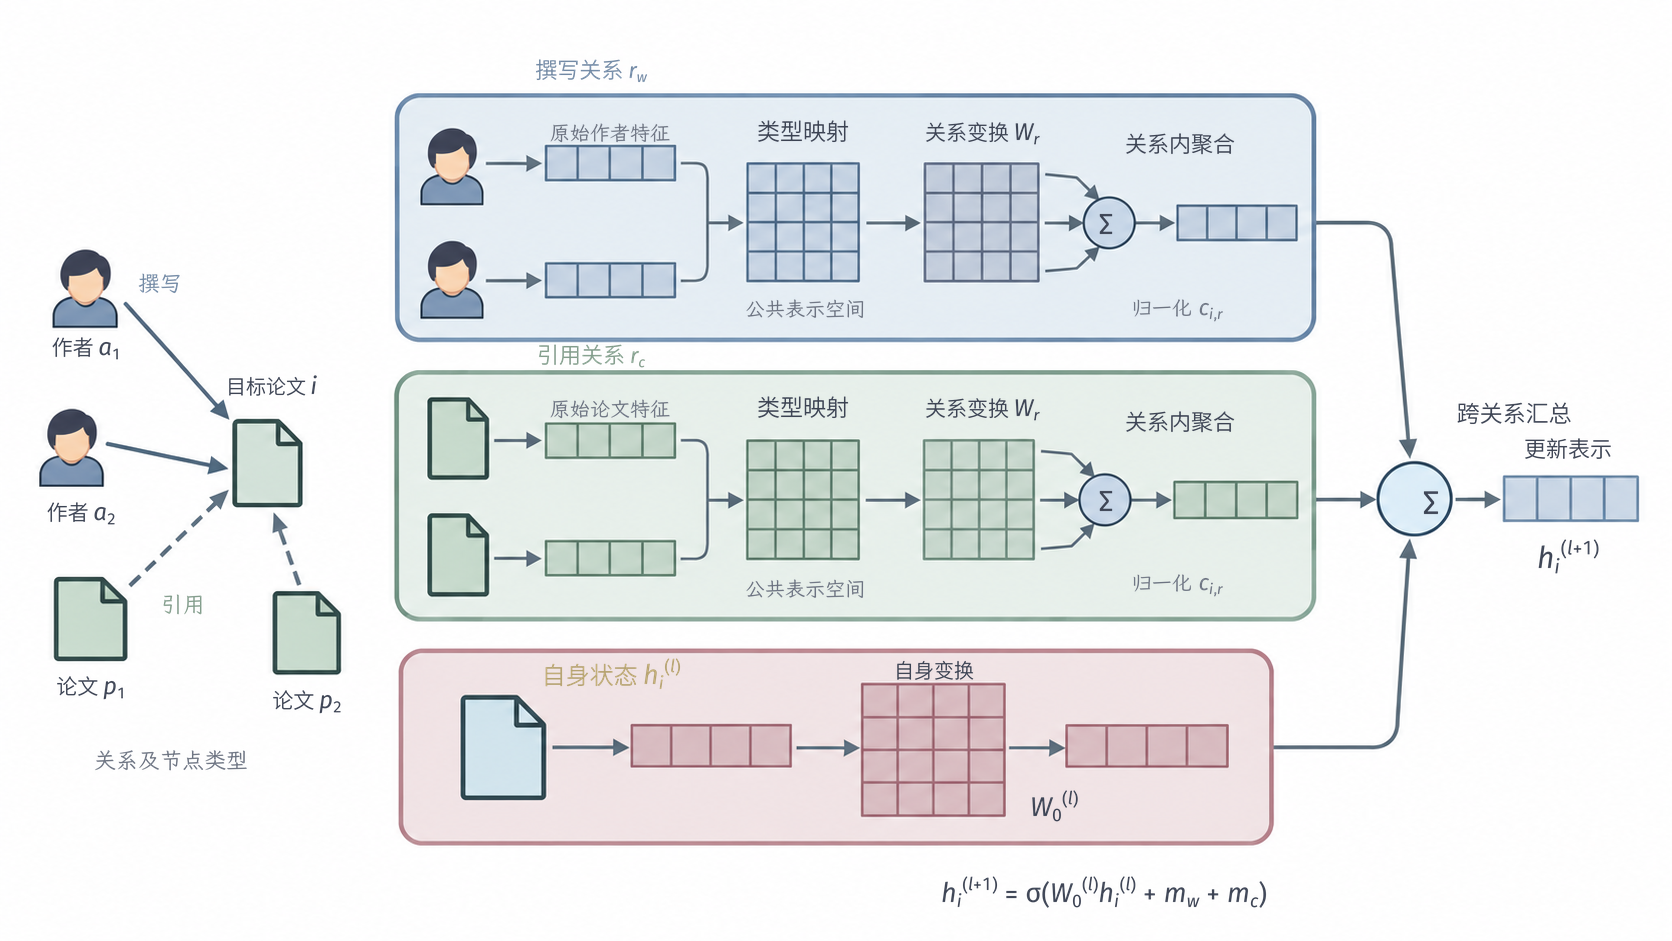
\includegraphics[width=141.563mm]{figures/03-models/02-neural-network-models/generated/gnn-typed-relations/figure.png}
  \caption{两类节点与两种关系的消息组织。作者的撰写关系和论文的引用关系分别经过类型映射与关系变换，再在各关系内部归一化聚合；两路结果$\bm m_{\mathrm w}$、$\bm m_{\mathrm c}$与独立的自身状态路径汇总，形成目标论文的新表示。各类型的特征组表示同类节点，不表示提前求和；矩阵网格只示意变换，不声明实际维度。}
  \label{fig:gnn-typed-relations}
\end{figure*}

\subsection{动态图}
\label{sec:gnn-dynamic}

社交互动、交易和设备关系会随时间改变。\term{动态图}（dynamic graph）把节点、边或属性的变化作为输入的一部分，模型不仅要处理当前关系，还要确定哪些历史在预测时可见。固定图上的十轮传播仍是同一个输入的十次内部计算，现实中的十个观测时刻则可能提供十份不同输入图。

一种表示是\term{图快照}（graph snapshot）：在时刻$t$取得$\mathcal{G}_t$与$\bm{X}_t$，先在每张快照中编码，再沿时间更新。对持续存在的节点可写为
\begin{equation}
  \bm{z}_{i,t}=\operatorname{GNN}(\mathcal{G}_t,\bm{X}_t)_i,
  \qquad
  \bm{s}_{i,t}=\operatorname{GRU}(\bm{s}_{i,t-1},\bm{z}_{i,t})\text{。}
  \label{eq:gnn-snapshot-dynamics}
\end{equation}
这里$\bm{z}_{i,t}$包含当前图中的邻域信息，$\bm{s}_{i,t}$维护跨时间历史。节点身份用于对齐相邻快照中的同一个对象；新节点的初态、节点消失后的状态保留与重现规则也要约定。快照间隔决定哪些短时事件被合并或遗漏。

另一种表示是带时间戳的\term{事件序列}（event sequence），例如第$q$个事件$(i_q,j_q,\tau_q,\bm{a}_q)$表示两个节点在时刻$\tau_q$发生互动。每个节点维护自己的记忆，在事件发生后更新相关状态。消息可以读取两端的事件前记忆、事件属性，以及距离该节点上次更新的时间间隔；不参与事件的节点记忆可以暂时保留。TGN以消息函数、消息聚合、记忆更新和时序表示等模块组织这一类计算\scite{rossi2020tgn}

预测互动是否发生时，应先用事件发生前的历史评分，再用实际发生的事件更新记忆。这样的先后顺序使评分只读取当时的历史，随后到达的事件再进入记忆。批量事件处理也要明确是否能读取同批中较早的事件；同一时刻事件的处理应采用约定的同时更新或已有先后关系，使事件次序对应实际观测含义。

图~\ref{fig:gnn-dynamic-before-update}把内部传播、观测时间与事件先后三种顺序分开。下半部的评分位于消息和记忆更新之前，正是避免把待预测事件提前写入历史的关键。

\begin{figure*}[htbp]
  \centering
  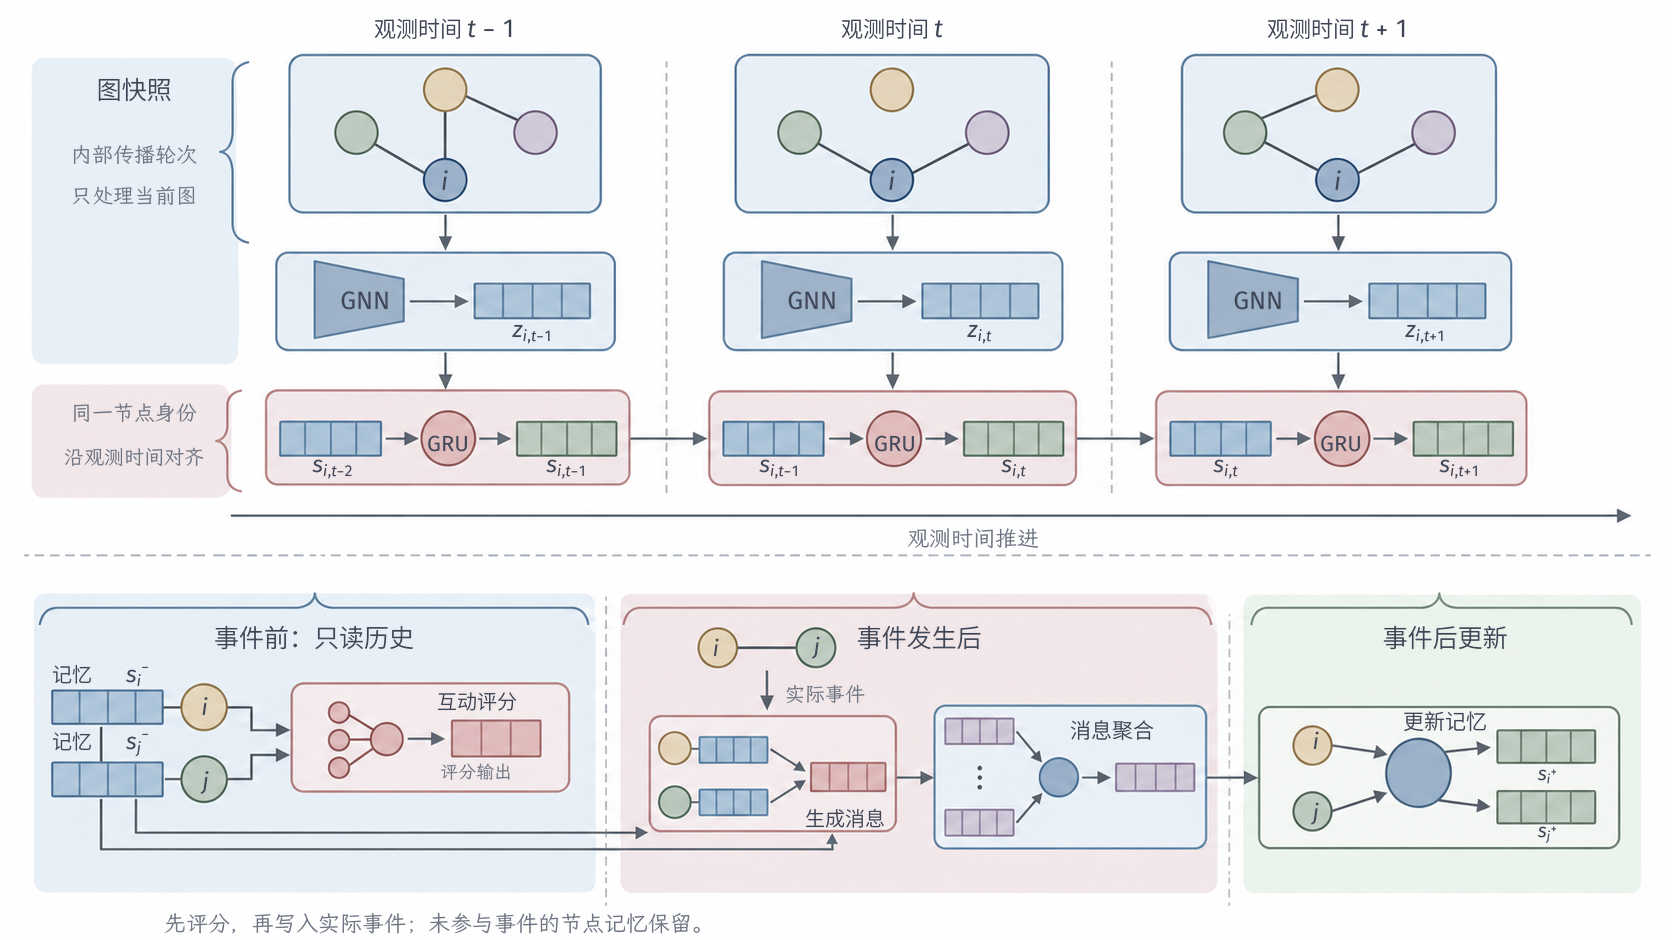
\includegraphics[width=141.563mm]{figures/03-models/02-neural-network-models/generated/gnn-dynamic-before-update/figure.png}
  \caption{动态图的两种时间组织。上半部区分固定快照中的内部传播与同一节点沿观测时间的GRU状态演化；下半部先用事件前记忆评分，实际事件到达后才生成消息、聚合并更新参与节点。未参与事件的节点保留记忆。}
  \label{fig:gnn-dynamic-before-update}
\end{figure*}

训练时可沿快照或事件展开反向传播，并在长流中按需要截断。评估未来事件时按时间划分，状态只由约定的可见历史推进；评估新节点时还要额外检查训练阶段是否已经接触其信息。内部传播深度、历史记忆长度和观测时间间隔共同影响计算，但衡量的是三种不同范围。

\subsection{高阶关系}
\label{sec:gnn-higher-order}

一次多人合作对应一个参与者集合，单条普通边只能描述两个对象。\term{超图}（hypergraph）用\term{超边}（hyperedge）表示同时连接多个节点的关系。记$\mathcal{H}=(V,\mathcal{E})$，其中$\mathcal{E}$是节点子集的集合；一条超边$S_a\subseteq V$保留这次关系的完整参与组。将它拆成所有成对边，可能无法区分“一次三人合作”与“三次两人合作”。

图~\ref{fig:gnn-hyperedge}展示一种计算表示：先让节点向超边聚合，再让超边把结果传回参与节点。将每条超边作为额外对象，会得到节点与关系对象构成的二部图；超边属性及非线性变换可以放在中间状态上。
\begin{figure*}[htb]
  \centering
  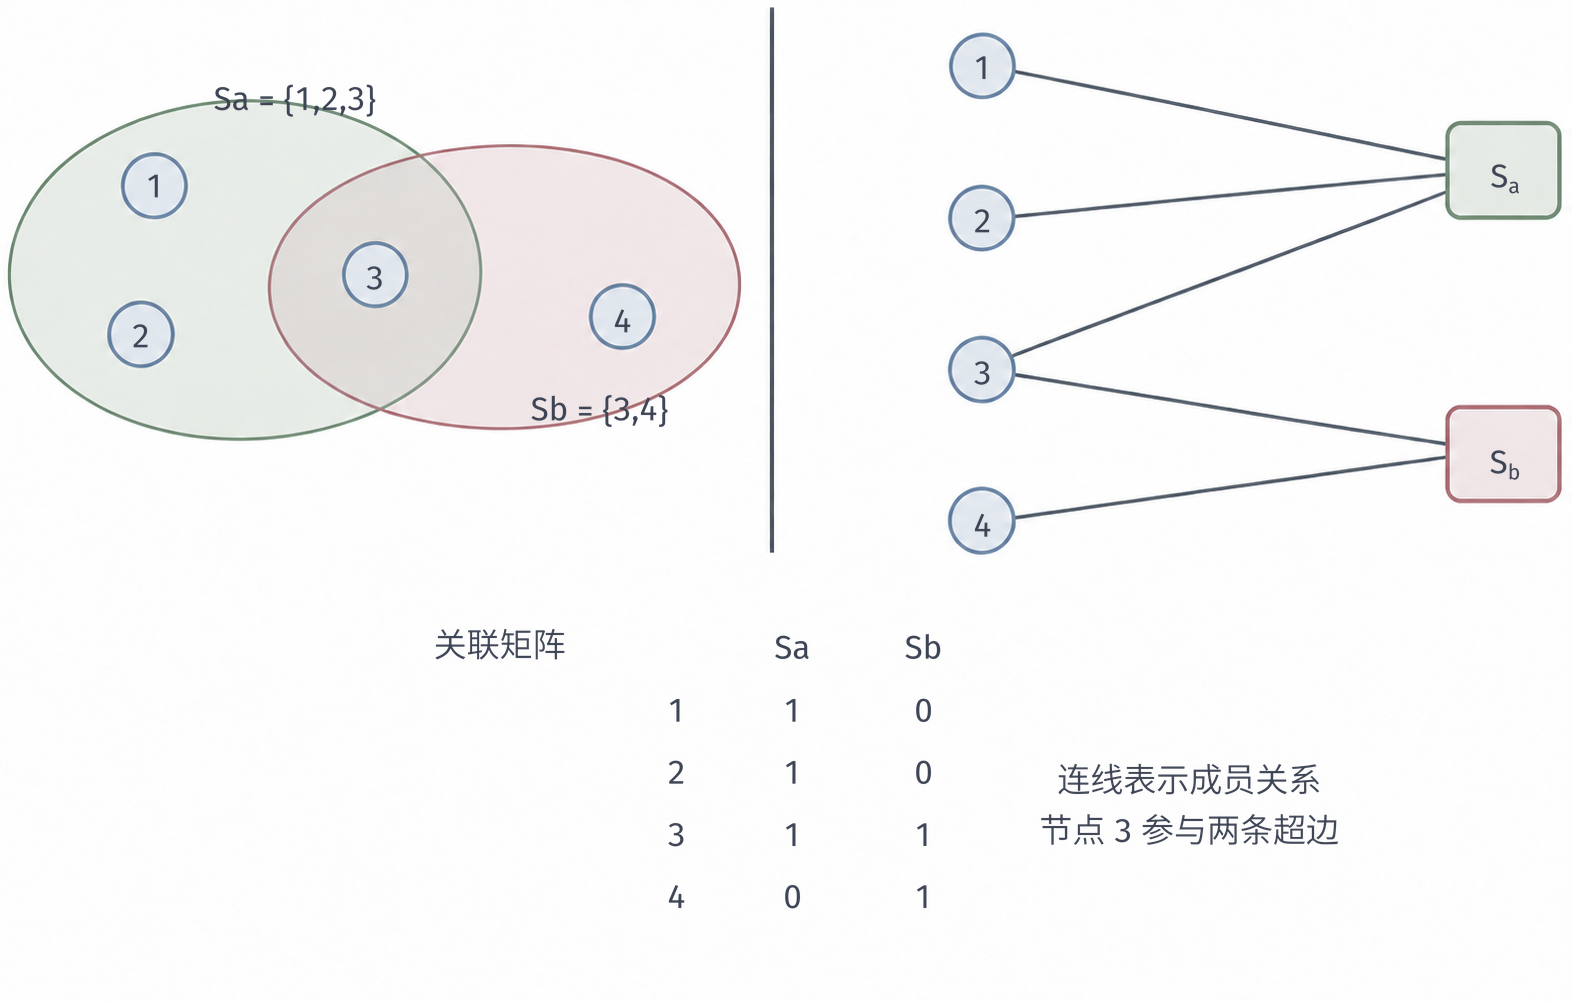
\includegraphics[width=133.096mm]{figures/03-models/02-neural-network-models/generated/gnn-hyperedge/figure.png}
  \caption{超边及其关联表示。左侧一条超边$S_a$连接节点1、2、3，另一条超边$S_b$连接节点3、4。右侧将超边画成方框，以连线表示参与关系；下方$4\times2$关联矩阵用同一组0／1关系把“集合、二部图、矩阵”对应起来。方框保存关系状态，原始参与者仍由圆形节点表示。}
  \label{fig:gnn-hyperedge}
\end{figure*}

令\term{关联矩阵}（incidence matrix）$\bm{B}\in\{0,1\}^{n\times h}$记录节点是否属于超边，$h=|\mathcal{E}|$，$\bm{B}_{i,a}=1$表示$i\in S_a$。设超边权重为$w_a>0$，$\bm{W}_e=\operatorname{diag}(w_1,\ldots,w_h)$，节点度$d_i=\sum_a\bm{B}_{i,a}w_a$，超边大小$s_a=\sum_i\bm{B}_{i,a}$。对非空超边及非孤立节点，一个归一化的传播为
\begin{equation}
  \bm{H}'=\sigma\!\left(
    \bm{D}_v^{-1/2}\bm{B}\bm{W}_e\bm{D}_e^{-1}
      \bm{B}^{\top}\bm{D}_v^{-1/2}\bm{H}\bm{\Theta}\right)\text{，}
  \label{eq:gnn-hypergraph-layer}
\end{equation}
其中$\bm{D}_v=\operatorname{diag}(d_i)$、$\bm{D}_e=\operatorname{diag}(s_a)$，$\bm{\Theta}$是特征变换矩阵。关联矩阵转置把节点信息汇到超边，关联矩阵再将结果送回节点；HGNN采用了这一类归一化超图卷积\scite{feng2019hgnn}

记录完整参与组后，还需要检查计算是否保留了这些组的差别。上述线性传播可以合成一个节点间矩阵（式\eqref{eq:gnn-hypergraph-layer}）。若两张超图产生相同矩阵，这一层也不能保留它们不同的组关系。任务依赖具体组时，可以在合成节点传播矩阵前保留超边状态、属性或组内非线性，使组关系继续进入输出。

另一类\term{高阶图网络}（higher-order graph neural network）把节点组作为状态对象，例如为节点对维护$\bm{h}_{i,j}$，使网络能够组合单节点状态难以保留的关系。它通过节点组索引安排状态与交互，可以由原图构造这些组，也可以读取已知高阶关系。Morris等将这种思路与高阶WL方法联系起来\scite{morris2019higherorder} 若显式维护所有$k$元节点组，状态数可达$O(n^k)$；选取部分子结构或局部组可以降低代价，但相应的区分能力也要重新说明。

\subsection{几何关系与对称性约束}
\label{sec:gnn-geometric}

原子或物体除了连接关系，还可能具有坐标$\bm{r}_i\in\mathbb{R}^{3}$。若把绝对坐标直接送入普通前馈消息函数，平移或转动物体就可能改变标量属性预测。几何任务需要另外指定对称性：能量等标量通常要求对整体平移和旋转不变；预测的位移或力则应随坐标系一起旋转。

令$\bm{r}'_i=\bm{Q}\bm{r}_i+\bm{t}$，其中$\bm{t}\in\mathbb{R}^{3}$是平移，正交矩阵$\bm{Q}$满足$\bm{Q}^{\top}\bm{Q}=\bm{I}_3$。相对位移随$\bm{Q}$作同一正交变换，距离$\lVert\bm{r}_i-\bm{r}_j\rVert_2$保持不变。用距离和其他不变属性产生标量消息，再用标量系数乘相对位移，就能构造等变的坐标更新。一个EGNN式的层可写为
\begin{equation}
  \begin{aligned}
    \bm{m}_{i\leftarrow j}
      &=\phi_e(\bm{h}_i,\bm{h}_j,
        \lVert\bm{r}_i-\bm{r}_j\rVert_2^2,\bm{a}_{i,j}),\\
    \bm{r}'_i&=\bm{r}_i+
      c_i\sum_{j\in N(i)}(\bm{r}_i-\bm{r}_j)\phi_r(\bm{m}_{i\leftarrow j}),\\
    \bm{h}'_i&=\phi_h\!\left(\bm{h}_i,\sum_{j\in N(i)}\bm{m}_{i\leftarrow j}\right)\text{。}
  \end{aligned}
  \label{eq:gnn-egnn}
\end{equation}
$\phi_r$输出标量，$c_i$是与坐标变换无关的归一化系数，$\bm{h}_i$此处由对所选欧氏变换不变的标量通道组成，边属性也具有相同不变性。EGNN使用距离构造消息，并用这种相对位移加权实现欧氏变换等变性\scite{satorras2021egnn}

证明只需跟踪各对象的变化。距离不变，所以消息及$\phi_r$不变；相对位移变为$\bm{Q}(\bm{r}_i-\bm{r}_j)$，整段坐标增量随$\bm{Q}$变换，加回$\bm{Q}\bm{r}_i+\bm{t}$后得到原更新结果的同一变换。邻接构造也须遵守该对称性，例如按距离阈值建边；若按固定坐标轴上的绝对位置选边，消息函数对称仍不足以保证整个模型对称。

正交矩阵还包括镜像反射。距离不变的模型因此可能无法区分互为镜像的手性构型；若目标会因镜像而改变，就需要只约束适用的对称群，并引入能保留相应方向关系的信息。所选对称群由目标决定：任务需要区分的方向关系应保留在输入与消息中。

若标量能量预测$\widehat E$可微且具有相应不变性，定义$\widehat{\bm{f}}_i=-\nabla_{\bm{r}_i}\widehat E$可以得到随旋转等变的力预测。能量与力由同一可微函数联系，具有相应数学一致性；预测精度再由监督、构型覆盖和数值计算检验。

\section{理论分析}
\label{sec:gnn-theory}

图结构改变了信息的传播路径，也改变了训练数据的依赖方式。讨论理论性质时，需要明确是在固定参数下计算状态、比较输入表示，还是从有限样本学习参数。这些对象分别对应状态求值、表示能力和参数学习，结论按其条件在本地建立。

\subsection{表达能力}
\label{sec:gnn-expressivity}
\label{sec:gnn-propagation-theory}

消息传递每轮只接触相邻表示；相同初始特征和相同邻域聚合结果可能使不同图始终不可区分。聚合是否保留多重集的数量与内容、传播轮次是否到达目标关系、读出是否保留所需结构，共同决定候选空间。GIN通过适当的单射聚合分析这类区分能力；特征域、更新及读出的条件共同确定它能区分的图对\scite{xu2019gin}

\subsubsection{过平滑：节点区分信息消失}
\label{sec:gnn-oversmoothing}

传播扩大感受野，却可能把不同节点的表示反复混在一起。\term{过平滑}（oversmoothing）指传播加深后，与节点差异有关的信息不断减少，以致任务需要的区分难以保留。不同层使用不同参数时也可能发生这种现象，任务需要的差异可以在各坐标尚未完全相等时已经受损。

\begin{figure}[htbp]
  \centering
  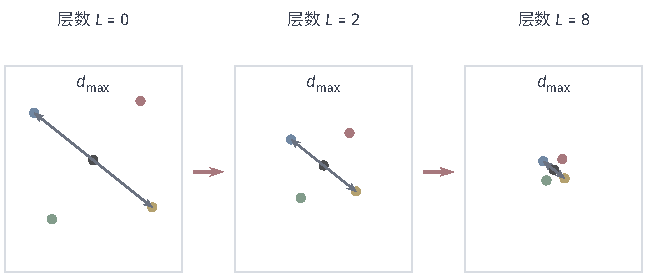
\includegraphics[width=109.580mm]{figures/03-models/02-neural-network-models/tikz/gnn-oversmoothing/figure.pdf}
  \caption{过平滑的二维投影示意。五种颜色始终代表同五个节点，位置只是人为构造的表示投影，并非t-SNE实验；随着传播层数增加，点间最大距离缩小，节点身份仍在但可供下游区分的表示差异逐渐消失。过平滑描述的是任务相关差异受损，不要求所有坐标严格相等。}
  \label{fig:gnn-oversmoothing}
\end{figure}

先看一个能够精确求解的简化模型：令激活与通道变换都为恒等，只反复计算$\bm{H}^{(l+1)}=\bm{S}\bm{H}^{(l)}$。假定非负无向图连通，并在每个节点加入正自环；对应$\bm{S}$具有唯一特征值1，其余特征值的绝对值小于1。定义单位向量
\[
  q_i=\frac{\sqrt{\widetilde d_i}}{\sqrt{\sum_j\widetilde d_j}}\text{，}
\]
则特征分解给出
\begin{equation}
  \bm{S}^L\bm{X}\longrightarrow\bm{q}\bm{q}^{\top}\bm{X},\qquad
  \lVert\bm{S}^L\bm{X}-\bm{q}\bm{q}^{\top}\bm{X}\rVert_F
    \leq\rho^L\lVert\bm{X}\rVert_F\text{，}
  \label{eq:gnn-linear-oversmoothing}
\end{equation}
其中$\rho$是其他特征值绝对值的最大值。证明依据是$\bm{q}$方向保持不变，其正交方向每次乘以绝对值至多为$\rho$的特征值。

极限中，每个节点只剩同一个特征向量的度相关倍数；除以$\sqrt{\widetilde d_i}$后便相同。若图不连通，每个连通分量保留一个相应方向；若没有破除周期的条件，例如无自环的二部图，状态还可能振荡。这里的极限与速度由连通性、归一化和破除周期的自环条件共同支持。

真实GCN的非线性、学习权重及跨层连接会改变这一纯线性传播，式\eqref{eq:gnn-linear-oversmoothing}先说明反复混合的基本机制。Oono与Suzuki在特定激活及参数范数条件下进一步分析了表示靠近低维子空间的速度，说明传播谱与权重尺度需要联合考察\scite{oono2020oversmoothing} 低频聚合在有限深度可能有用，任务需要保留的差异被过度削弱时才构成问题。

残差连接可以为旧表示保留额外路径，跨层拼接或读出可以直接读取较浅表示，初始特征注入则持续补充原始节点差异。这些设计改变了反复纯混合的形式。若恒等分支加入后又与传播共同归一化，表示仍可能持续混合；残差实际保留多少差异，取决于完整更新。

\subsubsection{过压缩：远处信息通过狭窄通路}
\label{sec:gnn-oversquashing}

另一种困难是节点需要利用许多远处对象，但这些信息只能经少量中间状态到达。\term{过压缩}（oversquashing）指大量关系信息沿传播路径汇入有限维状态或狭窄连接时，任务所需的远处影响难以有效传递。这里关注远期影响通过哪些通路、汇入多大状态；Alon与Yahav从这一信息瓶颈出发分析了长程图任务\scite{alon2021oversquashing}

一个二叉树例子能展示具体机制。设每个内部节点只把两个子节点的标量取平均，深度为$k$的$2^k$个叶子为$x_j$，则根状态为$h_{\mathrm{root}}=2^{-k}\sum_jx_j$，对单个叶子的导数为$2^{-k}$。距离增加时，每个叶子的单独影响迅速衰减；但根与各叶状态并没有被要求相同。图~\ref{fig:gnn-bottleneck}将汇聚树与图中的狭窄连接对应起来。

\begin{figure*}[htb]
  \centering
  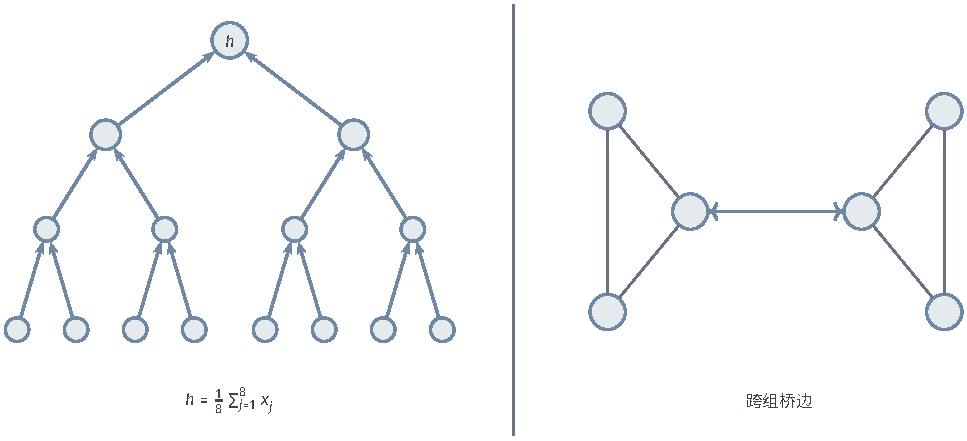
\includegraphics[width=163.791mm]{figures/03-models/02-neural-network-models/tikz/gnn-bottleneck/figure.pdf}
  \caption{两种信息汇聚瓶颈。左侧八个叶子经三层平均进入一个根状态，每个叶子的影响系数为$1/8$；右侧两组节点的跨组信息必须经过一条桥边。图不要求所有状态相同，强调的是大量信息必须经过较少的表示通路。}
  \label{fig:gnn-bottleneck}
\end{figure*}

若目标恰是叶子的平均，这种压缩就是所需计算；若目标要根据查询分别检索某个叶子，单一平均已经丢掉必要差别。因此，过压缩要相对于任务解释。压缩容量的分析需同时规定精度、噪声或连续性条件；无限精度实数与设备上的有限精度状态能够区分的历史数目不同。

增加状态宽度可以提供更多通道，增加传播轮次可以到达更远处，却也可能增加汇入同一状态的信息量。修改图结构、加入长程连接或全局读取，可以缩短路径并扩大跨区域通路；这些做法也改变了关系假设和计算量。残差主要保留已有信息路径，未必能解除一条桥边上的瓶颈。状态收敛、过平滑与过压缩因而需要分别诊断，再选择对应设计。

\subsection{收敛性}
\label{sec:gnn-convergence}

参数训练关心经验目标怎样随更新改进：有限层消息传递通常形成非凸经验目标。光滑、有下界且梯度按完整计算图求得时，合适步长可给出趋近驻点的速率；邻域采样、离散结构更新和非光滑算子需要额外分析。驻点速率控制所计算的梯度尺度，全局最优需要更强的目标条件。更新规则与速率条件见第\ref{chap:neural-network-training}章。

\subsubsection{状态收敛及其条件}
\label{sec:gnn-state-convergence}

不动点模型需要知道反复更新是否会停在确定的状态。\term{压缩映射}（contraction mapping）条件要求：对同一输入，两份状态经过更新后距离按小于1的固定比例缩小。比较距离针对整张图的状态，消息聚合和所有节点的更新共同进入这个比例。

固定图、输入与参数，若更新把非空闭状态域映回自身，并在同一范数下以非负统一比例$c<1$收缩，则任意该域内初态都趋于唯一状态$\bm h^*$，且
\begin{equation}
 \lVert\bm h^{(t)}-\bm h^*\rVert\leq c^t\lVert\bm h^{(0)}-\bm h^*\rVert.
 \label{eq:gnn-contraction-error}
\end{equation}
这给出了状态存在、唯一和迭代误差的结论（参考\BookTheoremRef{thm:analysis-banach-fixed-point}{第一卷“数学准备”的Banach压缩映射定理}）。

在同一收缩条件下，相邻状态差还给出可检查的后验误差证书：对$t\geq1$，$\lVert\bm{h}^{(t)}-\bm{h}^*\rVert\leq c(1-c)^{-1}\lVert\bm{h}^{(t)}-\bm{h}^{(t-1)}\rVert$。$c$接近1时，误差证书中的放大系数较大，同一相邻差对应较宽的最终误差上界；迭代速度与停止容差由此联系起来。

例如采用矩阵状态更新$\bm{H}'=\sigma(\bm{S}\bm{H}\bm{W}+\bm{B}_x)$，其中$\bm{B}_x\in\mathbb{R}^{n\times m}$为固定输入项。若$\sigma$是$L_\sigma$-Lipschitz的，则Frobenius范数下
\begin{equation}
  \lVert\bm{H}'_1-\bm{H}'_2\rVert_F
    \leq L_\sigma\lVert\bm{S}\rVert_2\lVert\bm{W}\rVert_2
      \lVert\bm{H}_1-\bm{H}_2\rVert_F\text{。}
  \label{eq:gnn-state-lipschitz}
\end{equation}
乘积小于1且状态域不变时，可应用这一收缩结论。未经归一化的求和传播可能因最大节点度增大而放大该上界；对称归一化的无向GCN传播满足$\lVert\bm{S}\rVert_2=1$。门控中的门值落在$[0,1]$时，完整导数还包含门随状态变化的项，收缩条件需把它们一并计入。

收缩保证的是固定参数下的状态计算。参数更新会改变$F_{\bm{\theta}}$，训练目标通常仍然非凸。状态不动点让当前参数的预测器可以确定求值，训练进展和新样本误差再分别评价。收缩也是充分条件而非必要条件，有限轮次模型本来就不要求以不动点定义输出。

\subsection{泛化性}
\label{sec:gnn-generalization}

\subsubsection{样本单位与图上的依赖}
\label{sec:gnn-sample-units}

对分子属性预测，一张分子图及其标签可以作为一个样本，图内节点允许相互依赖。若$N$张图独立同分布，前面学习理论中的样本量就是$N$，并不是所有原子数的总和。若多张图来自同一系统的连续快照，或由一张大图截取重叠片段，它们未必独立。

单张引用图上的节点分类具有另一种组织方式：输入结构与特征可以共享，节点标签及其邻域又相互关联。随机选若干标签做训练，并不把全部节点变成独立同分布图样本。固定图上的未标记节点风险可以采用直推分析；从一个图生成模型抽样时，需要把相应结构依赖写进假设。风险分析的样本量与依赖条件由这一抽样过程给定，节点数只有在对应假设中才具有相应统计含义。

邻域互不重叠时仍可能共享生成因素，独立性需要从数据产生过程检验。样本划分应对应未来使用：已知图上的剩余标签、全新图、全新节点和未来事件分别有不同的信息边界。比较不同模型时，必须固定这一边界。

\subsubsection{输入尺度、度与参数范数}
\label{sec:gnn-norm-generalization}

在独立整图设定下，结构怎样进入泛化分析，可以先从网络敏感度考察。考虑无偏置层$\bm{H}^{(l+1)}=\sigma(\bm{S}\bm{H}^{(l)}\bm{W}^{(l)})$，激活为1-Lipschitz且零点取零。对同一图上的两份特征，固定参数后有
\begin{equation}
  \lVert\bm{H}^{(L)}-\widetilde{\bm{H}}^{(L)}\rVert_F
    \leq\lVert\bm{S}\rVert_2^L
      \prod_{l=0}^{L-1}\lVert\bm{W}^{(l)}\rVert_2
      \lVert\bm{X}-\widetilde{\bm{X}}\rVert_F\text{。}
  \label{eq:gnn-feature-sensitivity}
\end{equation}
每层先用激活的Lipschitz性，再用矩阵乘法的范数界，逐层相乘即得。它控制固定结构下的输入扰动；若边同时改变，还必须增加传播算子变化的项。

未经归一化的邻接求和在非负加权无向图上满足$\lVert\bm{A}\rVert_2\leq d_{\max}$，其中$d_{\max}$是最大加权度。这个上界可能随深度以$d_{\max}^L$进入敏感度；标准对称归一化将传播的谱范数控制为1。归一化同时改变传播尺度与度、计数信息；任务是否需要这些信息，决定它与尺度控制之间的取舍。

读出又带来规模差别。平均读出满足$\lVert n^{-1}\bm{1}^{\top}\bm{H}\rVert_2\leq\lVert\bm{H}\rVert_F/\sqrt n$，求和读出的对应系数为$\sqrt n$。若每个节点输入范数不超过$B_x$，则$\lVert\bm{X}\rVert_F\leq B_x\sqrt n$；平均与求和对应的输出上界分别消去或保留节点规模。宽度、偏置、注意力评分和关系参数还会改变其余常数，需按实际模型计入。

对权重扰动也可逐层计算。只改变第$k$层权重时，当前误差至多为$\lVert\bm{S}\rVert_2\lVert\bm{H}^{(k)}\rVert_F\lVert\Delta\bm{W}^{(k)}\rVert_2$，后续层再乘各自的尺度界。逐个替换所有层并用三角不等式，可以建立输出对全部参数的统一Lipschitz上界。深度影响重复传播和误差累积，参数共享限制自由度，却不取消同一参数反复使用的敏感度。

\subsubsection{从参数约束到风险界}
\label{sec:gnn-risk-bound}

把敏感度接到泛化分析，还需要给出样本怎样抽取、允许哪些参数以及损失怎样计量。下面给出一个便于检查条件的整图预测界，承接统计学习部分的一致收敛思路，不假定独立节点。

\begin{theorem}[有界参数图预测的覆盖界]
\label{thm:gnn-cover-generalization}
设$Z_1,\ldots,Z_N$是独立同分布的整图及标签样本。预先固定的参数域$\bm{\Theta}\subseteq\mathbb{R}^{p}$包含在半径$B_\theta>0$的欧氏球内，损失$\ell_{\bm{\theta}}(Z)\in[0,1]$关于样本可测，且对全部允许的样本与参数有
\[
  |\ell_{\bm{\theta}}(Z)-\ell_{\widetilde{\bm{\theta}}}(Z)|
    \leq a\lVert\bm{\theta}-\widetilde{\bm{\theta}}\rVert_2
\]
其中$a>0$为预先给定的统一常数。记期望风险$R(\bm{\theta})=\mathbb{E}\ell_{\bm{\theta}}(Z)$与经验风险$\widehat R_N(\bm{\theta})=N^{-1}\sum_q\ell_{\bm{\theta}}(Z_q)$。对任意预先固定的$\varepsilon>0$与$\delta\in(0,1)$，以至少$1-\delta$的概率，
\begin{equation}
  \begin{aligned}
    \sup_{\bm{\theta}\in\bm{\Theta}}
      |R(\bm{\theta})-\widehat R_N(\bm{\theta})|
      &\leq2\varepsilon\\
      &\quad+\sqrt{\frac{p\log(1+2B_\theta a/\varepsilon)
        +\log(2/\delta)}{2N}}\text{。}
  \end{aligned}
  \label{eq:gnn-cover-risk}
\end{equation}
\end{theorem}
\begin{proof}
欧氏球内的参数集合有半径$\varepsilon/a$的覆盖，中心取自$\bm{\Theta}$，覆盖数至多为$(1+2B_\theta a/\varepsilon)^p$。对每个中心的有界损失使用Hoeffding不等式，再用并合界，得到平方根项。任意参数到最近中心的损失差不超过$\varepsilon$，期望风险与经验风险各增加至多$\varepsilon$，合计得到$2\varepsilon$。
\end{proof}

这个界把独立图数、参数自由度、参数范围和统一敏感度放在同一表达式中。前面的范数推导可以在限定图规模、特征尺度与网络结构后帮助构造$a$；图拓扑及度会通过传播算子进入它。统一常数须覆盖全部允许样本和参数；训练图上测到的局部梯度，只描述其中一部分状态，分析还需建立共同尺度界。

原始交叉熵无上界，超出上述$[0,1]$损失范围；可使用有界替代损失，或在额外概率下界及尺度处理后重新分析。参数覆盖界给出满足这些条件时的统一保证，数值可能较松；实际测试误差仍由对应数据评价。Rademacher复杂度可以更细地利用样本和函数约束，算法稳定性则研究替换一个完整图样本后学习结果的变化；采用哪一种工具，都必须与样本单位和损失条件对应。

结构设计还影响拟合偏差。更强的对称性减少无关自由度，却可能排除任务需要的方向差异；聚合保留更多输入差异，可以让后续函数利用这些差异，实际预测仍需要数据与学习过程支持。残差提供额外路径时，其Lipschitz上界常出现$1+$分支尺度，梯度直达路径与候选函数族的复杂度分别计量，分支相加的尺度仍需纳入上界。

测试图比训练图更大、节点度分布不同，或关系类型及标签机制变化时，已经改变了输入分布。共享更新可以在新规模上执行，仍不保证超出训练范围的误差保持不变。同分布整图泛化、固定图直推以及跨规模或分布预测，对应不同数据条件；比较结果据各自信息范围和样本来源解释。

\section{常见应用}
\label{sec:gnn-applications}

以下三个任务使用不同预测对象，但都需要把可见关系、编码器、输出和监督对应起来。具体领域的特征工程、评估协议和应用方法留给应用卷，这里展示一个完整模型如何接入任务。

\subsection{节点分类}
\label{sec:gnn-application-node}

以论文引用网络为例，每篇论文是节点，内容向量是$\bm{x}_i$，引用是有向边。若任务允许同时读取引用与被引用的信息，可以分别使用两个方向，或明确把图无向化；后一种选择会丢掉方向差别。内容编码器只使用约定的可见文本，类别标签另放在监督集合中。

一个基本模型是两层GCN：$\bm{H}^{(1)}=\operatorname{ReLU}(\bm{S}\bm{X}\bm{W}^{(0)})$，节点概率矩阵为$\bm{P}=\operatorname{softmax}_{\mathrm{row}}(\bm{S}\bm{H}^{(1)}\bm{W}^{(1)})$，Softmax逐行作用。按式\eqref{eq:gnn-node-loss}仅在训练节点上计算交叉熵，反向更新两层权重。两轮传播使每个预测可以读取两跳以内的内容与连接信息。

直推设定下，验证和测试节点的无标签特征与连接可以按协议参与编码；类别标签则保存在各自评估集合，训练只读取规定的监督标签。若预测未来发表的论文，则训练时不得使用未来引用边和文本，内容编码、建图及归一化也须按当时可见的信息重建。相同两层公式可以用于两种设定，但它们回答的是不同泛化问题。

还应比较只使用内容的前馈基线，以检查关系是否提供了额外信息。邻居类别常相近时聚合可能有用；关系跨越类别边界时，分开自身与邻居、处理方向或关系类型，可以保留类别边界两侧的不同信息，效果按实际引用与标签关系检验。

\subsection{连接预测}
\label{sec:gnn-application-link}

关系网络中，编码器先在可见图上产生$\bm{z}_i=\bm{h}_i^{(L)}$，解码器再为候选节点对评分。无向连接可用$s_{i,j}=\bm{z}_i^{\top}\bm{z}_j$；有向关系可用$s_{i,j}=\bm{z}_i^{\top}\bm{R}\bm{z}_j$，一般矩阵$\bm{R}$允许交换端点后得分变化。多关系任务可把$\bm{R}$改为类型相关参数。

训练批次包含已知正连接及从候选范围抽出的负样本，按式\eqref{eq:gnn-edge-loss}联合更新编码器与评分参数。未观察到的边并不一定是真实负例，它可能只是尚未记录；采样范围、正负比例和缺失机制决定目标的含义。Sigmoid得分对应所用采样任务的类别比例；解释为实际连接概率时，需要处理现实比例与缺失机制的差异。

评估保留连接时，需要从编码图中移除这些边及其反向副本，避免编码器直接读取答案。训练正边是否在给该边评分时仍参与编码，也应说明；可以另外划分用于消息传递与用于监督的正边，或在批次中临时屏蔽目标边，使训练输入与目标评估口径对应。对未来连接，则先用历史图评分，事件发生后再更新动态图状态。

预测时对所需候选评分和排序。全部节点对数量为$O(n^2)$，即使编码器在稀疏图上计算，枚举全部候选仍可能昂贵。候选生成与负样本改变评价难度，比较模型时需要固定它们；随机负例与实际候选可能有不同难度，最终关系判断由部署候选上的相应指标检验。

\subsection{整图属性预测}
\label{sec:gnn-application-graph}

以分子属性预测为例，节点表示原子，边表示化学键。原子种类、形式电荷等作为节点属性，键类型等作为边属性，消息函数据此产生固定宽度向量。传播若干轮后，通过式\eqref{eq:gnn-readout}形成分子表示，再用前馈输出头预测标量，按式\eqref{eq:gnn-graph-loss}学习。输入编码、消息函数、更新与输出头共同接受梯度。

读出选择要与属性性质对应。随体系大小累积的量可以采用节点贡献求和的结构，强调整体分子组成；与规模不直接成比例的量可以使用平均或更一般的可学习读出。节点贡献求和编码了可加性的结构假设，局部表示能否充分表达真实属性仍需按任务检验。

只有二维连接关系时，网络不知道同一分子不同空间构型的坐标差别。若目标依赖三维构型，需要把预测时可得的坐标与几何关系纳入，并按第~\ref{sec:gnn-geometric}节处理对称性。近邻空间图传递空间接近关系，化学键图传递键连接；两种通路分别记录其输入语义。

训练和测试按完整分子划分；同一分子的多种构型或高度相近的结构是否跨划分，需要与目标使用场景对应。仅随机分图可能主要检查近似结构间的插值，按结构族划分则考察更远的迁移。验证图用于选择传播深度、宽度与读出，测试图用于评价相应设定下的预测误差。

\section{本章小结}
\label{sec:gnn-summary}

对象数量和连接不规则时，共享消息沿给定边交换表示，对称聚合把数量可变的邻域变成固定宽度状态。节点表示随重编号等变，整图读出对重编号不变。多轮传播扩大可见范围，聚合、状态宽度与拓扑则共同决定能否保留任务需要的信息。

频率响应若用多项式规定，可以按节点邻域稀疏传播；GCN的低阶谱推导与归一化邻域层展示了这一联系。采样、内容加权和多重集合区分解决不同问题；循环共享则须区分有限展开与不动点求解。关系类型、时间、高阶关系和几何对称性进一步规定了哪些信息必须保留。

状态梯度沿前向读取反向回传，并汇合为共享参数的导数；训练趋于驻点需要目标、梯度估计与步长满足相应条件。固定参数的状态收敛保证求值，过平滑描述节点差异消失，过压缩描述远处信息受到狭窄通路限制。节点、连接和整图任务各自指定输入关系、对称性及读出，再以匹配的监督和划分检验。共享计算使网络能够接入新图，样本依赖、图分布与参数尺度则共同约束新图预测的证据。

\paragraph{扩展阅读}
Bishop与Bishop的教材及本章各类图网络原论文，可用于比较谱滤波与局部消息传递。教材中的统一计算视角与各模型的具体聚合、滤波和读出可以相互对照；置换对称、多重集区分及图级和节点级数据依赖，则对应本章的结构、表达与学习问题\scite{bishop2024deep}

\chapter{Transformer}
\label{chap:transformer}

理解“猫追狗”时，动词位置需要同时知道前后的对象；续写“猫追”时，同一位置却只能依据已经给定的前缀。两个任务都需要读取其他位置，允许读取的内容不同。第\ref{sec:rnn-attention}节的循环注意力已经让解码器按当前需求读取源表示，源表示和解码状态仍逐步形成。对于已经完整给定的输入，怎样让各位置直接交换信息？对于尚未产生的输出，又怎样使每次读取符合预测当时的已知范围？

Transformer用注意力选择读取的来源，用层间堆叠反复组合读取结果。顺序通过位置表示和连接约束进入计算，监督目标决定哪些输出接受误差反馈；保存多少位置、建立多少连接又决定相应的计算与存储。本章围绕这组关系建立网络结构和梯度计算，再比较位置、注意力、前馈与连接方式的扩展，分析学习结论的条件，并将它们接到分类、转换、生成和图像任务中。

\section{Transformer概述}
\label{sec:transformer-overview}

一段输入完整给定后，各位置可以先形成表示，再同时读取彼此，下一层使用这些读取结果。Transformer按这种方式组织位置交互；注意力的发展解释了怎样选择信息，架构的发展则解释了如何把读取接到不同预测任务。并行计算带来的便利还伴随着逐位置表示的存储和读取成本。

\subsection{从循环计算到位置间读取}
\label{sec:transformer-core-idea}

循环注意力中的查询来自解码状态，候选表示来自编码状态；它使每一步可以重新选择上下文，却保留了状态递推。\term{自注意力}（self-attention）把查询和候选表示都取自同一组输入：每个位置根据自身表示，选择同一序列中其他位置的信息。例如，在“这部电影并不精彩”中，表示“精彩”的位置可以直接读取“并不”，形成带有上下文的表示。否定上下文能否进入最终判断，取决于学到的权重、被读取的值及后续变换；直连使这条信息路径在结构上可用。

\term{Transformer}是一类以注意力进行位置间交互、以逐位置前馈网络进行特征变换的网络。一次读取使用该层入口已有的表示，因而同层各位置可以同时更新；下一层再读取这些新表示。稠密自注意力为允许读取的位置对建立直接路径。来自多个位置的信息汇入加权混合，任务所需的差别还要由值特征和后续变换保留。

\subsection{注意力机制的发展}
\label{sec:transformer-attention-history}

注意力机制始终围绕一个问题展开：当前计算应该优先使用哪些信息？早期视觉模型通过选择观察位置分配处理资源，后来的序列模型通过可学习权重读取已有表示。沿着这两条相互交汇的路线，可以看清注意力如何从局部选择机制发展为Transformer中的基本运算。

\paragraph{早期视觉注意力：选择在哪里观察}
1985年，Koch与Ullman提出选择性视觉注意力的计算模型：不同视觉特征共同形成\term{显著图}（saliency map），即标出各位置有多突出的空间分布；模型选出突出位置，再抑制已选位置，使注意转向其他区域。这类模型解释观察资源的空间分配；后文的查询、键和值则描述已有表示之间的加权读取\scite{koch1985attention}

神经网络随后被用于学习观察策略。Schmidhuber与Huber在1991年的工作中，用神经控制器移动“人工中央凹”，即中心精细、外围粗略的局部观察区域，以逐步找到和跟踪目标。控制器借助学到的环境模型改进移动轨迹，观察位置由这一策略产生\scite{schmidhuber1991attention} 2014年，Mnih等用循环网络整合多次局部观察，并学习下一次观察的位置。这种先采样位置、再读取局部输入的方式属于\term{硬注意力}（hard attention）；论文从高斯策略中采样连续位置坐标。局部读取操作无法沿常规可微路径直接优化，观察策略因而用策略梯度训练\scite{mnih2014attention}

\paragraph{机器翻译：从固定上下文到软对齐}
序列转换遇到的是另一种信息瓶颈：编码器已经读完整句，但若只把一个固定向量交给解码器，每个目标词都要从同一压缩结果中恢复细节。Bahdanau、Cho与Bengio于2014年发布、2015年发表于ICLR的工作保留所有源位置的编码状态，在生成每个目标词之前，用此前的解码状态重新为这些源状态评分。得分经Softmax变成权重，再加权求和，形成随生成步变化的上下文。多个源位置共同提供信息，权重随翻译目标学习，聚合运算可微；这就是\term{软注意力}（soft attention）形成的软对齐\scite{bahdanau2015}

例如翻译“猫追狗”时，预测cat与预测dog所需的源信息不同，读取权重可以随之改变；“对齐”表示目标步与源位置之间学到的软对应，其监督来自翻译目标。这项工作中的加性注意力用一个小前馈网络评估两种状态是否匹配，具体公式已见式\eqref{eq:rnn-additive-attention}。每次读取随目标步改变，源表示的形成和目标状态的更新则继续使用循环递推。

2015年，Luong等系统比较了直接点积、带参数的双线性形式等评分方式，并区分读取全部源位置的全局注意力与只读取一个窗口的局部注意力。这使“怎样评分”和“允许读取哪些位置”成为可分别选择的设计；局部方案规定候选窗口，窗口内部仍可对多个位置软加权\scite{luong2015} 同年，Xu等的Show, Attend and Tell将基于内容的注意力用于图像描述：生成不同词时，语言解码器可以对不同图像区域分配权重，论文同时研究了软聚合与随机硬选择。被读取对象由源词变为图像区域，按当前需求选择信息的作用保持不变\scite{xu2015showattend}

\paragraph{自注意力：从读取另一序列到建立内部关系}
注意力还可以用来联系同一序列中的位置。2016年，Cheng等在用于机器阅读的LSTM记忆网络中保存此前词元的表示，并让当前词元通过注意力读取这些记忆，建立序列内部关系。这种\term{序列内注意力}（intra-attention）是自注意力的一种早期实现，网络仍保留循环更新；这项设计改变了读取来源，循环更新继续安排表示形成的次序\scite{cheng2016reading}

上述模型改变了不同环节：硬选择和软聚合规定怎样取出信息，加性和点积规定怎样评分，交叉与自注意力规定表示来自哪组位置。评分方式、信息来源和读取范围可以组合；第\ref{sec:transformer-attention}节将用查询、键和值统一描述这些角色，再展开Transformer采用的计算形式。

\subsection{Transformer的提出与演进}
\label{sec:transformer-architecture-history}

注意力机制使解码器可以反复读取源表示，但这些表示最初仍由循环网络产生。1997年的LSTM通过记忆单元与控制门改善长距离信息的保留和梯度传递，更新仍沿时间进行\scite{hochreiter1997} 2014年，Sutskever等用LSTM编码器—解码器进行序列转换，将输入压缩到固定维表示\scite{sutskever2014seq2seq} 第\ref{sec:transformer-attention-history}节介绍的软对齐进一步减轻了固定表示的瓶颈，循环递推却仍限制整段输入表示的并行形成。

2017年，Vaswani等在机器翻译中提出Transformer：源端以自注意力形成上下文，目标端以因果自注意力形成前缀表示，再用交叉注意力读取源端。位置表示提供顺序，多头读取形成多组聚合，逐位置前馈层变换特征。这一设计把位置间的循环更新改为注意力读取与层间堆叠，为已知序列提供批量矩阵计算方式\scite{vaswani2017}

% 三条完整引文的边栏高度大于正文段落，预留共同阅读空间。
\Needspace{165mm}
形成表示的读取规则也开始服务于不同预训练目标。2018年，GPT用因果Transformer进行语言模型预训练，再适配有监督任务\scite{radford2018gpt} 同年发布、2019年发表于NAACL的BERT用双向编码器从被遮蔽的输入恢复词元，形成可用于多种理解任务的表示\scite{devlin2019} 2020年发表的T5研究把任务统一为文本输入到文本输出，采用编码器—解码器组织条件生成\scite{raffel2020t5} 第\ref{sec:transformer-common-architectures}节将比较这些架构；预训练数据和迁移范式由相关章节展开。

\subsection{与RNN/LSTM的比较}
\label{sec:transformer-recurrent-comparison}

与RNN/LSTM相比，关键变化在于历史信息的组织方式。普通循环网络把过去压缩进固定宽度状态；LSTM增加记忆与门，改善保留方式，但仍需经中间时间步传递。稠密自注意力保存各位置的表示，让当前位置直接读取所需历史。远处证据因此可沿一层连接到达，同时更多位置的键和值需要留存。配有注意力的循环模型还可以保存源位置表示，其历史存储和读取应把这一额外部分计入。表~\ref{tab:transformer-rnn-comparison}固定长度和宽度，比较三种基础结构。

并行计算的条件是所需输入已经给定。训练自回归模型时，真实目标序列已知，可以一次送入移位后的目标，并用掩码限制各位置读取；生成时，下一个词元尚未确定，仍需根据已有前缀产生它，再继续下一步。已知序列的各位置表示可以并行形成；自回归输出则按新词元到达的次序逐步延长。

全局读取也有成本。设序列长为$n$，表示宽度为$d$，常规多头注意力的各头总宽度与$d$同阶，一层自注意力的位置对计算需要$O(n^2d)$次算术操作，投影另需$O(nd^2)$。直接保存各头权重需要$O(hn^2)$个元素，其中$h$为头数。与固定宽度的循环状态相比，Transformer保存和读取了更多逐位置信息；后文将区分减少连接、改变聚合公式和改善存储方式三种路线。适用场景包括文本、连续时间观测和图像块等可表示为向量序列的输入，这些任务的顺序、局部关系和可见范围由位置表示、连接及输入协议继续规定。

\begin{table*}[htbp]
  \centering
  \small
  \begin{tabular}{@{}p{28mm}p{39mm}p{40mm}p{48mm}@{}}
    \toprule
    比较维度 & 基础RNN & LSTM & 稠密Transformer自注意力 \\
    \midrule
    历史表示 & 固定宽度隐藏状态 & 隐藏状态与记忆单元 & 每层保留逐位置键和值 \\
    顺序来源 & 时间递推 & 时间递推及门控 & 位置表示与可见性约束 \\
    已知整段的计算 & 同层沿时间串行 & 同层沿时间串行 & 同层位置可并行，层间依赖仍在 \\
    远位置的结构路径 & 经中间时间步，$O(n)$ & 经中间时间步，$O(n)$ & 允许直连时，一层内$O(1)$ \\
    单层整段算术量 & $O(nd^2)$ & $O(nd^2)$，门增加常数 & $O(n^2d+nd^2)$ \\
    生成时的历史存储 & $O(d)$ & $O(d)$ & 常规KV缓存为$O(nd)$ \\
    \bottomrule
  \end{tabular}
  \caption{固定输入及隐藏宽度同阶为$d$、序列长为$n$的结构比较。历史存储按单层、单样本统计，省略训练激活和参数；Transformer各头总宽度与$d$同阶。最短连接路径不保证实际依赖一定学会，算术量也不直接等于运行时间。三者在标准自回归生成时都逐步产生输出。}
  \label{tab:transformer-rnn-comparison}
\end{table*}
\FloatBarrier

\section{网络结构}
\label{sec:transformer-structure}

下面沿输入表示、位置读取、逐位置变换与任务输出说明计算。以长度为$n$的一段输入建立共同记号。隐藏表示宽度为$d$，网络块数为$L$，第$l$个块后的矩阵为$\bm H^{(l)}\in\mathbb R^{n\times d}$，按行存放各位置的列向量，即$\bm H_{i,:}^{(l)}=(\bm h_i^{(l)})^{\top}$。括号上标表示层间更新编号，位置使用下标。这里讨论单个样本；批量计算另加样本维，并分别处理有效长度。

\subsection{输入表示与位置编码}
\label{sec:transformer-input}

注意力接收向量，原始输入需要先转为统一宽度。文本中的\term{词元}（token）是分词系统采用的离散单位，可以是词、子词或符号。设词表大小为$v$，位置$i$的词元编号为$u_i$，嵌入矩阵为$\bm E\in\mathbb R^{v\times d}$，则$\bm e_i=(\bm E_{u_i,:})^{\top}$。同一词元的各次出现从同一行参数取出内容向量；之后的网络将它与位置和上下文组合，产生各次出现自己的隐藏表示。

若输入是$\bm x_i\in\mathbb R^p$的连续观测，可以用$\bm e_i=\bm W_{\mathrm{in}}\bm x_i+\bm b_{\mathrm{in}}$投影到$d$维，其中$\bm W_{\mathrm{in}}\in\mathbb R^{d\times p}$。图像可以先分为小块，再把每块的像素或前端特征展平并投影。三种接口都产生注意力可读取的向量。文本顺序、实际时间间隔、图像坐标及观测缺失可以加入这些向量或相应读取规则，使任务所需关系也进入模型。

在“猫追狗”和“狗追猫”中，词元相同，动词两侧的角色却交换了。网络需要从输入中获得这个顺序差别。递推式$\bm h_i=f(\bm h_{i-1},\bm x_i)$已经使第$i$步接收到“处理过前$i-1$项”的状态，交换输入会改变后续计算。自注意力的共享投影只看到内容向量与内容匹配，矩阵的第几行并不会自动变成网络可用的特征。仅使用词元嵌入时，同一个词元面对相同的内容集合；将位于动词之前或之后的信息加入计算后，模型才有区分施事与受事的输入依据。同一词元多次出现时，位置关系还帮助网络区分每次出现的作用。

这一缺口可以用计算性质精确表达。以不含位置表示和顺序掩码的自注意力为例，对输入行施加置换矩阵$\bm P$，查询、键、值也同步重排，得分矩阵变为$\bm P\bm S\bm P^{\top}$。逐行Softmax随之重排，因此
\begin{equation}
  \operatorname{SA}(\bm P\bm H)
  =\bm P\operatorname{SA}(\bm H)\text{。}
  \label{eq:transformer-permutation}
\end{equation}
共享的逐位置前馈层和归一化保留这一等变性。若再做平均读出，整段输出便对重排不变；“猫追狗”和“狗追猫”可能因只有相同内容向量而无法区分。因果掩码使位置只能读取此前输入，改变了上述置换条件。它规定连接范围；位置距离则还需要编码或由具体网络计算获得。某些因果模型可以借助边界和层间计算学习部分顺序，任务需要哪些关系仍由输入和结构决定。若输入本来是无序集合，保留置换等变性可以避免把保存编号引入预测。

\term{位置编码}（positional encoding）把元素所在位置或位置之间的关系加入表示计算。最直接的做法为每个位置设置$\bm p_i\in\mathbb R^d$，并令
\begin{equation}
  \bm h_i^{(0)}=\bm e_i+\bm p_i\text{。}
  \label{eq:transformer-input-position}
\end{equation}
这称为\term{绝对位置编码}（absolute positional encoding）：位置$i$本身有一个表示。可学习位置表与词元嵌入共同训练，正弦位置编码则按固定函数产生。相加要求维度一致；原始Transformer对词元嵌入乘以$\sqrt d$，以调整内容与位置的相对尺度，其他输入接口则可按自身尺度配置。

把这一步落到实际序列上，取“猫／追／猫”，暂把每个汉字当作一个词元；实际模型也可能采用子词等其他切分。两个“猫”查询同一行嵌入参数，因此位置1和3的内容向量相同。为便于手算，令嵌入宽度为4，猫的嵌入为$(0.20,-0.10,0.40,0.30)^{\top}$，追的嵌入为$(0,0.50,-0.20,0.10)^{\top}$。下列数值为便于复算而构造的教学嵌入。图中的词元矩阵$\bm E_{\mathrm{seq}}$与位置矩阵$\bm P_{\mathrm{pos}}$均按序列位置排列，形状为$3\times4$，以区别于完整词表参数表和置换矩阵。

图~\ref{fig:transformer-position-example}把内容与位置分成两条计算路径。假设词表给“猫”和“追”分配的编号分别是7和12，左图用词元编号$7,12,7$查嵌入表；中图从序列的先后顺序得到位置序号$1,2,3$，并代入四维正弦位置向量$\bm p_i=(\sin i,\cos i,\sin(0.01i),\cos(0.01i))^{\top}$，角度以弧度计。位置序号与词表编号不同，两个“猫”虽然查到同一个内容向量，仍会得到不同的位置向量。右图将两路表示按对应坐标相加，输出形状保持为$3\times4$。逐坐标相加保持四维宽度；沿特征维拼接则得到八维，需要相应修改后续接口。第\ref{sec:transformer-position-extensions}节会解释这些频率如何推广到任意偶数宽度，以及如何改为表示相对距离。

\begin{figure*}[htbp]
  \centering
  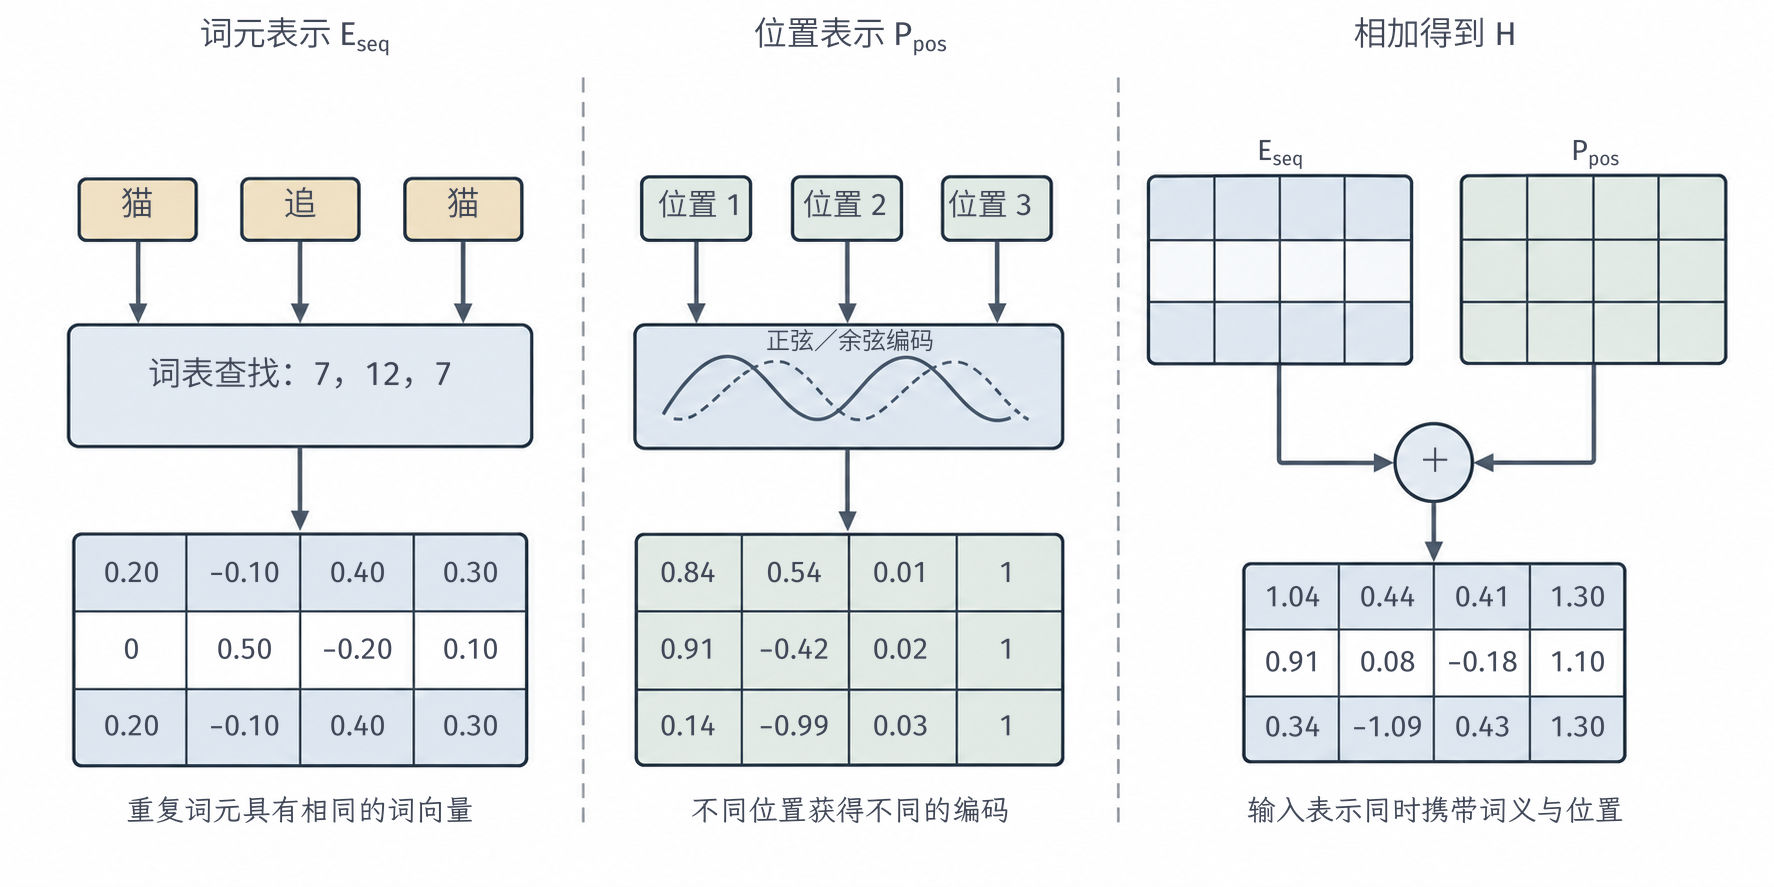
\includegraphics[width=150.199mm]{figures/03-models/02-neural-network-models/generated/transformer-position-example/figure.png}
  \caption{序列“猫／追／猫”的输入构造。左图用词元编号查嵌入表，中图把位置序号代入正弦、余弦函数，右图将两组$3\times4$表示逐元素相加。三个矩阵的行均按输入位置排列，每格是一个特征值。两个“猫”共享内容向量，位置向量及最终表示却不同。词元编号和嵌入为教学设定；位置向量按弧度计算，数值保留两位小数，位置矩阵的最后一列显示相同是舍入所致。}
  \label{fig:transformer-position-example}
\end{figure*}
\FloatBarrier

位置差异需要以能够留在后续表示中的方式编码。仅把编号$i$填在各坐标上，会遇到均值消除问题。例如，后文第\ref{sec:transformer-residual-normalization}节介绍的层归一化会减去一行的均值；若输入只加$i\bm1$并立即按行归一化，这个位置常数就会被消去。不同频率或可学习坐标提供了更丰富的位置差异。内容与位置进入同一表示后，训练才能据任务目标调整它们的组合与读取。

不等长序列可以填充到共同形状，真实位置由有效集合或长度记录。注意力排除填充键，池化只汇总真实位置，损失只统计有效监督位置。若将多段独立文本装入同一矩阵，也需限制跨段读取，并明确位置编号的重置方式；矩阵中相邻不等于任务中连续。

\subsection{注意力层}
\label{sec:transformer-attention}

第\ref{sec:transformer-attention-history}节已经介绍了注意力怎样根据当前需求读取信息。可以先把一次读取类比为查字典：手中待查的词是\term{查询}（query, Q），字典里用于匹配条目的词头是\term{键}（key, K），找到条目后读取的释义是\term{值}（value, V）。查询提出当前需求，键提供匹配特征，值提供被取出的内容；注意力中的键因此是表示向量，数组下标只负责存放它。

注意力把这种查询推广为连续的软匹配。输入经可学习投影得到查询、键和值，查询与键的连续得分再变成权重；多个值依权重共同形成输出。投影参数随训练调整，匹配方式也随之改变。这里把输入固定为“猫／追／狗”：更新“追”的表示时，网络需要结合谁在追、追的是谁；更新“猫”时，所需的上下文组合又可能不同。同一个位置在读取别人和被别人读取时承担不同作用，查询与键用于评分，值用于输出，三者不需要具有相同含义。

设查询输入为$\bm H_{\mathrm q}\in\mathbb R^{n_q\times d}$，被读取输入为$\bm H_{\mathrm s}\in\mathbb R^{n_s\times d}$。暂省略偏置，单头投影为
\begin{equation}
  \begin{aligned}
    \bm Q&=\bm H_{\mathrm q}\bm W_{\mathrm q},\qquad
    \bm K=\bm H_{\mathrm s}\bm W_{\mathrm k},\\
    \bm V&=\bm H_{\mathrm s}\bm W_{\mathrm v}\text{，}
  \end{aligned}
  \label{eq:transformer-qkv}
\end{equation}
其中$\bm W_{\mathrm q},\bm W_{\mathrm k}\in\mathbb R^{d\times d_k}$，$\bm W_{\mathrm v}\in\mathbb R^{d\times d_v}$；$\bm Q$、$\bm K$分别有$n_q$、$n_s$行和$d_k$列，$\bm V\in\mathbb R^{n_s\times d_v}$。若两侧宽度不同，只需分别调整投影的输入维度。评分公式规定权重怎样计算，信息来源规定键值来自哪里，可见范围规定哪些位置参与，头数则规定并行读取的组数。这些设置可以在一次注意力计算中共同使用。

\subsubsection{缩放点积注意力}

\term{缩放点积注意力}（scaled dot-product attention）把所有查询与键的点积转为权重，再聚合值。令$\bm M\in\mathbb R^{n_q\times n_s}$为固定掩码：允许读取时$\bm M_{i,j}=0$，禁止读取时为$-\infty$。一次前向计算为
\begin{equation}
  \begin{aligned}
    \bm S&=\frac{\bm Q\bm K^{\top}}{\sqrt{d_k}}+\bm M,\\
    \bm A_{i,j}&=\frac{\exp(\bm S_{i,j})}
      {\sum_{t=1}^{n_s}\exp(\bm S_{i,t})},\\
    \bm Z&=\bm A\bm V\text{。}
  \end{aligned}
  \label{eq:transformer-attention}
\end{equation}
$\bm S,\bm A\in\mathbb R^{n_q\times n_s}$，$\bm Z\in\mathbb R^{n_q\times d_v}$。第$i$行输出是$\bm z_i=\sum_j\bm A_{i,j}\bm v_j$，其中$\bm v_j=(\bm V_{j,:})^{\top}$。Softmax沿键的位置归一化，每一行只在允许读取的位置上分配总量为1的权重；各行独立归一化，并不要求每列之和也为1。

分母$\sqrt{d_k}$针对点积宽度增加带来的波动。若改用$d_k$或固定常数，缩放后波动会有不同的宽度依赖。点积累加了$d_k$个乘积，即使坐标尺度不变，累加值的波动也可能增长。下面用一个初始化时的简化模型说明这种增长，并把它与Softmax的梯度联系起来\scite{vaswani2017}

\paragraph{从坐标方差得到缩放因子}
暂时省略位置下标，设$\bm q,\bm k\in\mathbb R^{d_k}$相互独立，各自坐标也相互独立，且每个坐标均值为0、方差为1。令$s=\bm q^{\top}\bm k$。对第$r$个乘积，有
\[
  \mathbb E[q_rk_r]=\mathbb E[q_r]\mathbb E[k_r]=0,\qquad
  \mathbb E[(q_rk_r)^2]=\mathbb E[q_r^2]\mathbb E[k_r^2]=1\text{。}
\]
不同坐标乘积之间的协方差为0，因此
\begin{equation}
  \begin{aligned}
    \mathbb E[s]&=\sum_{r=1}^{d_k}\mathbb E[q_rk_r]=0,\\
    \operatorname{Var}(s)
      &=\sum_{r=1}^{d_k}\operatorname{Var}(q_rk_r)
        +2\sum_{r<t}\operatorname{Cov}(q_rk_r,q_tk_t)\\
      &=d_k,\\
    \operatorname{Var}\!\left(\frac{s}{\sqrt{d_k}}\right)&=1\text{。}
  \end{aligned}
  \label{eq:transformer-attention-scale-variance}
\end{equation}
标准差是方差的平方根，所以点积的典型波动尺度为$\sqrt{d_k}$。用它作分母，可以消去由宽度引起的增长；若除以$d_k$，方差反而变成$1/d_k$，宽度越大，得分就越被压向0。

\paragraph{得分尺度怎样影响Softmax}
将一行得分记为$\bm s$、权重记为$\bm a=\operatorname{softmax}(\bm s)$，其导数为
\begin{equation}
  \frac{\partial a_j}{\partial s_t}
      =a_j(\delta_{j,t}-a_t)\text{，}
  \label{eq:transformer-softmax-scale-gradient}
\end{equation}
其中$\delta_{j,t}$在$j=t$时为1，否则为0。若某个得分远大于其余得分，对应权重接近1，其他权重接近0，这些导数都会很小。对于只有两个键的情况，令$\Delta=s_2-s_1$，则$a_2=1/(1+e^{-\Delta})$，且$\partial a_2/\partial\Delta=a_2(1-a_2)$；当$|\Delta|$很大时，导数趋于0。

例如，取$d_k=64$，若未缩放的两个得分为$(0,8)$，第二个权重约为$0.9997$，对得分差的导数约为$0.00034$；除以$\sqrt{64}=8$后，得分为$(0,1)$，权重约为$0.7311$，对缩放后得分差的导数约为$0.1966$。若比较反传到同一个原始点积差$r$的梯度，还要计入缩放的导数：
\[
  a_2=\frac{1}{1+\exp(-r/\sqrt{d_k})},\qquad
  \frac{\partial a_2}{\partial r}
    =\frac{a_2(1-a_2)}{\sqrt{d_k}}\text{。}
\]
在本例$r=8$时，该导数约为$0.1966/8=0.02458$，仍大于未缩放时的$0.00034$。这组教学数值说明缩放如何缓解由维度放大造成的过早饱和；具体输入的导数由得分差决定，注意力仍可形成尖锐权重。减去行最大值控制指数的数值范围，缩放改变得分差；两项操作承担不同作用。

独立、零均值和单位方差是上述初始化模型的条件。训练后的查询与键可能相关，坐标尺度也会改变；自注意力还让二者来自同一输入，因此实际得分需要按当前表示评价。$1/\sqrt{d_k}$控制的是宽度带来的系统性变化，并不保证任意训练阶段的得分方差恰好为1。

\begin{example}[同一查询在不同可见范围内的读取]
  \label{ex:transformer-attention-numerical}
  对“猫／追／狗”中第2个位置“追”发起的查询，设$d_k=1$、$q_2=1$，三个词元的键依次为$0,\log2,0$，值依次为$(1,0)^{\top}$、$(0,2)^{\top}$、$(1,1)^{\top}$。这些是投影后的教学数值，不表示真实模型必然这样关注句子。三个缩放得分为$(0,\log2,0)$，取指数后为$(1,2,1)$，归一化得到权重$(1/4,1/2,1/4)$。输出为
  \[
    \bm z_2=\tfrac14(1,0)^{\top}+\tfrac12(0,2)^{\top}
                    +\tfrac14(1,1)^{\top}
             =(1/2,5/4)^{\top}\text{。}
  \]
  这个向量是“追”的新表示，不是直接选出一个词。三份二维值的贡献都进入这一表示，各自比例由权重给出。若改成因果读取，当前位置尚不能看到“狗”，得分变成$(0,\log2,-\infty)$，权重相应变为$(1/3,2/3,0)$，输出为$(1/3,4/3)^{\top}$。因果掩码使Softmax在前两个位置上重新归一化，原来的四分之一、二分之一比例也随候选范围改变。
\end{example}

图~\ref{fig:transformer-attention}先画出输入经三组参数投影得到查询、键和值，再把“追”的读取拆成评分、归一化和加权求和。查询与键决定“读多少”，值决定“读到什么”。键参与评分，值进入加权输出，混合结果可以与所有输入值都不同。损失因此同时影响评分权重和值特征，后文分别推导两条梯度路径。

\begin{figure*}[htbp]
  \centering
  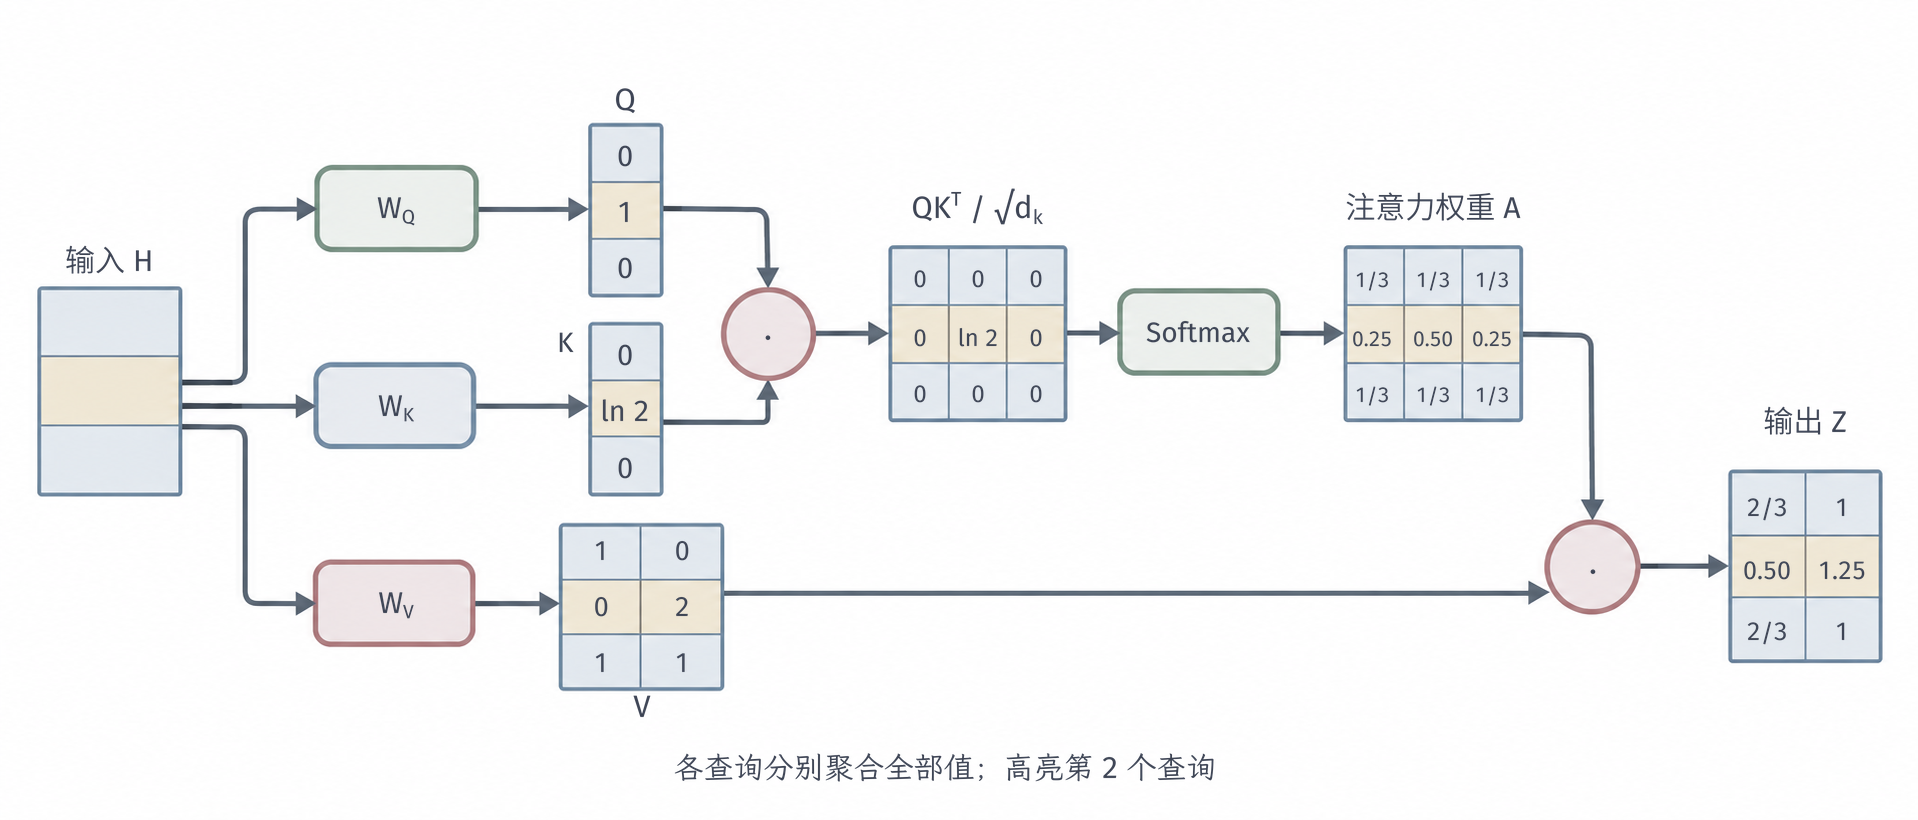
\includegraphics[width=162.391mm]{figures/03-models/02-neural-network-models/generated/transformer-attention/figure.png}
  \caption{三个位置的缩放点积注意力，突出显示“追”这一查询。输入分别经三组投影产生查询$\bm Q$、键$\bm K$和值$\bm V$，三者各行依次对应猫、追、狗。突出显示的查询为$q_2=1$，与全部键匹配得到三个得分。Softmax按查询行产生权重矩阵，随后与值矩阵相乘得到各行输出；突出显示的一行权重为$(0.25,0.50,0.25)$，输出为$\bm z_2^{\top}=(0.50,1.25)$。浅色单元格示意矩阵数据，强调色标明同一查询的评分、权重与输出；$d_k=1$、$d_v=2$，数值均为教学设定。}
  \label{fig:transformer-attention}
\end{figure*}
\FloatBarrier


\subsubsection{自注意力：同一序列内部读取}

上下文理解需要让一个输入位置结合其他输入位置。自注意力在式\eqref{eq:transformer-qkv}中取$\bm H_{\mathrm q}=\bm H_{\mathrm s}=\bm H$，查询、键和值都由同一组位置投影，得分矩阵为$n\times n$。三组投影各有参数；即使共享输入，通常也有不同的查询、键和值，只有特定参数设置才会得到$\bm Q=\bm K=\bm V$。为使三组线性投影可以逐项核对，图中取教学输入$\bm H=\bm I_3$，三组投影矩阵分别取为图示的$\bm Q$、$\bm K$、$\bm V$；独热输入让投影矩阵的每一行可直接对应图示数值，真实词元则通常使用前面定义的内容与位置表示。图~\ref{fig:transformer-self-attention}单独展开“追”的查询：三个位置提供值，按对应权重合成输出。中图权重表按查询位置排列，第2行就是$(0.25,0.50,0.25)$。若同一组键对应的另外两个查询取$q_1=\log_2 3$、$q_3=-1$，就分别得到第1行$(0.2,0.6,0.2)$和第3行$(0.4,0.2,0.4)$。查询不同，即使候选键值相同，读取也可以不同。整段输入可见时，各有效位置都在候选集合内，具体读取比例仍随查询与键改变。

\begin{figure*}[htbp]
  \centering
  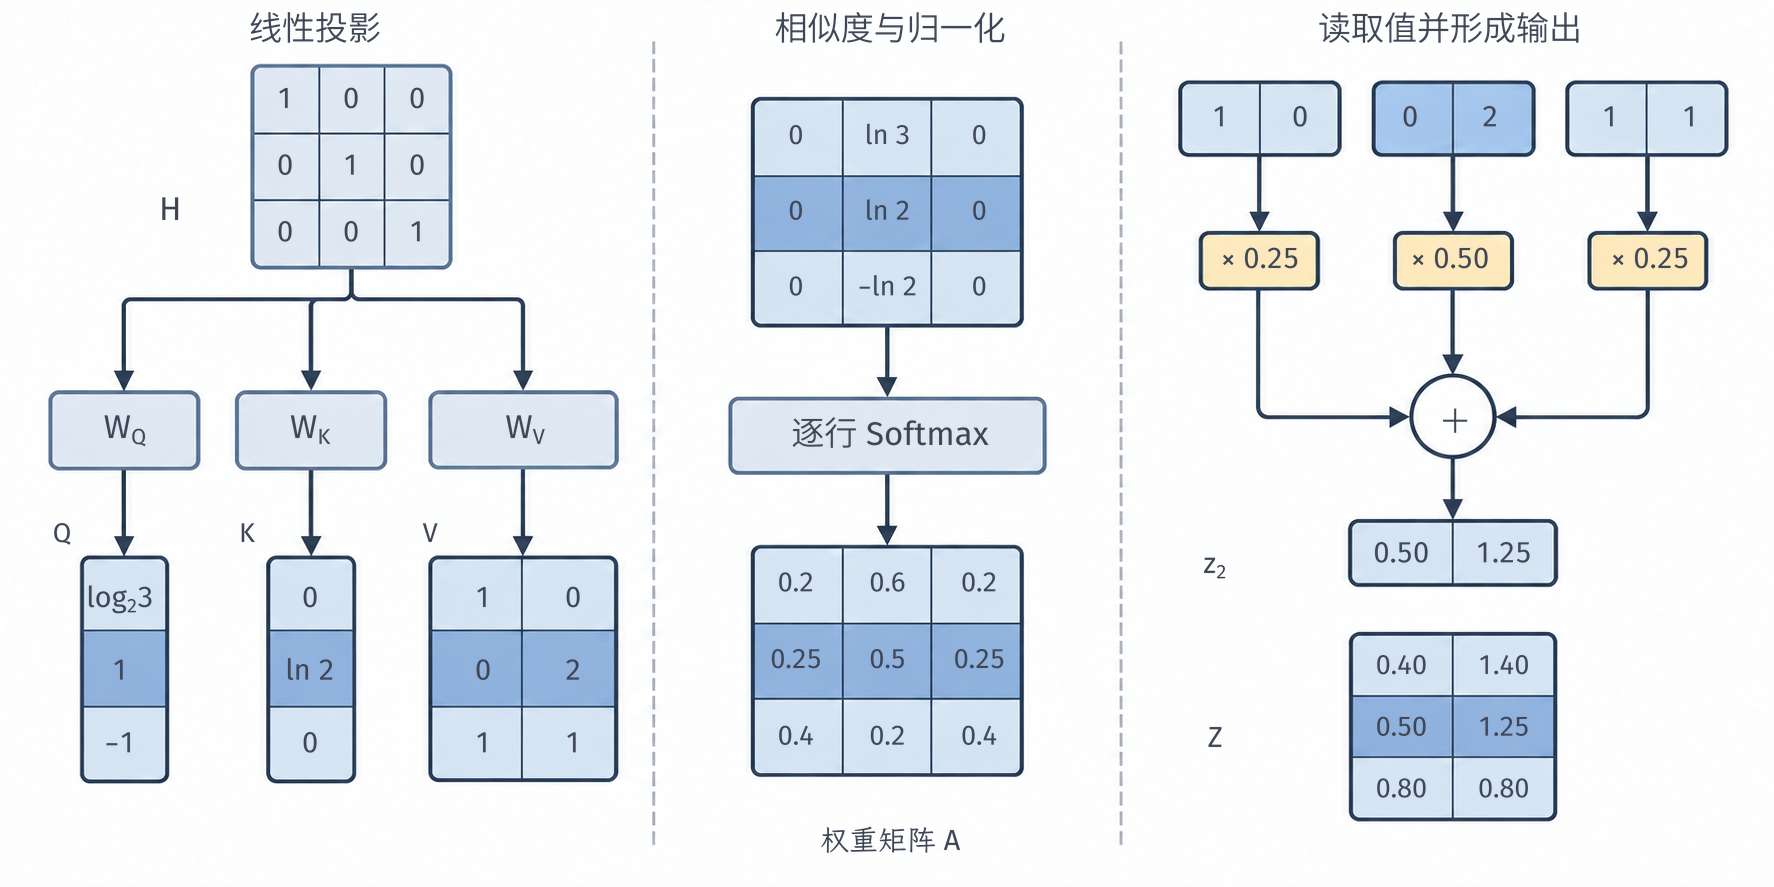
\includegraphics[width=150.199mm]{figures/03-models/02-neural-network-models/generated/transformer-self-attention/figure.png}
  \caption{同一序列“猫／追／狗”上的自注意力。左图将教学输入$\bm H=\bm I_3$分别投影为查询、键和值；中图展示得分及逐行Softmax，行对应查询位置，列对应被读取位置。右图展开第2个查询，将三个二维值按$(0.25,0.50,0.25)$加权，得到$\bm z_2^{\top}=(0.50,1.25)$；下方矩阵汇总各查询分别计算的输出。$d_k=1$、$d_v=2$，所有数值为教学设定。}
  \label{fig:transformer-self-attention}
\end{figure*}
\FloatBarrier

\subsubsection{交叉注意力：从另一组表示读取}

目标序列需要读取源序列时，双方长度和职责通常不同。\term{交叉注意力}（cross-attention）让$\bm H_{\mathrm q}$提供查询，另一组$\bm H_{\mathrm s}$提供键和值，得分矩阵为$n_q\times n_s$。例如翻译目标当前位置用自己的状态提出查询，读取已编码的源句；每个查询产生一行输出，被读取侧提供键和值。以翻译“猫／追／狗”为例，图~\ref{fig:transformer-cross-attention}同时展开两个已知目标输入位置BOS和cat。BOS位置的输出用于预测cat，cat位置的输出用于预测chases；这两个目标状态产生两行查询，三个源编码状态产生三行键和值。源、目标长度不同，输出仍按目标查询排列，因此$\bm A$为$2\times3$，而$\bm Z$只有两行。

为了逐项算出一次交叉读取，取$d_k=1$，设目标投影后的查询为$\bm Q=(0,1)^{\top}$，源投影后的键为$\bm K=(0,\ln8,0)^{\top}$，值沿用前例的三个二维向量。BOS的三个得分都为0，Softmax给出$(1/3,1/3,1/3)$；cat的得分为$(0,\ln8,0)$，取指数得到$(1,8,1)$，归一化后为$(0.1,0.8,0.1)$。两行分别乘以同一个$\bm V$，得到$\bm z_1=(2/3,1)^{\top}$和$\bm z_2=(0.2,1.7)^{\top}$。后者对应cat发起的查询，供该目标位置后续预测使用。这一教学构造演示连续加权；真实翻译权重由训练形成，可能同时读取多个源位置。交叉注意力也可用于一种模态读取另一种模态；信息来源改变，不要求评分公式改变。

\begin{figure*}[p]
  \centering
  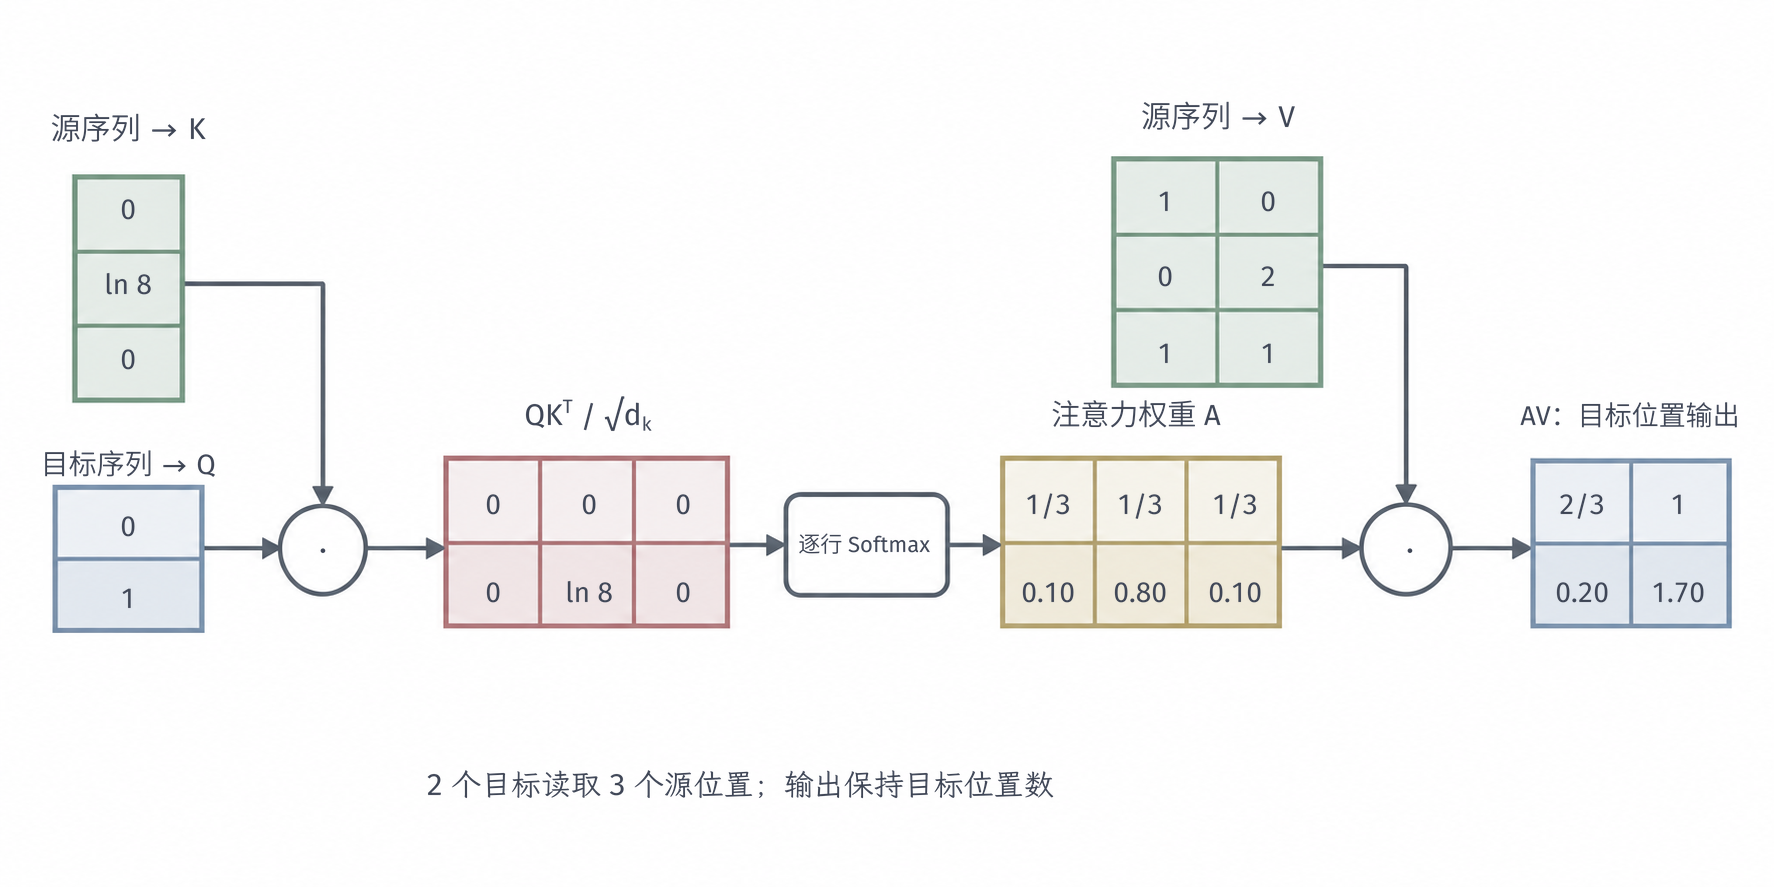
\includegraphics[width=150.199mm]{figures/03-models/02-neural-network-models/generated/transformer-cross-attention/figure.png}
  \caption{两条不同序列的交叉注意力。目标输入BOS／cat的状态投影为两行查询，源输入猫／追／狗的编码状态分别投影为三行键和值。得分与权重矩阵的行对应目标查询、列对应源词元，因此形状均为$2\times3$；权重矩阵乘以$3\times2$的值矩阵后，输出为$2\times2$。较深的单元格突出cat这一目标位置从查询、评分、归一化到输出的对应关系。$d_k=1$，所有投影数值均为教学设定。}
  \label{fig:transformer-cross-attention}
\end{figure*}
\FloatBarrier

\subsubsection{因果注意力：只读取已知前缀}

同一序列也可能包含尚不能用于当前预测的未来内容。\term{因果注意力}（causal attention）通常指带因果掩码的自注意力，规定位置$i$只能读取$j\leq i$的键值。图~\ref{fig:transformer-causal-attention}把“猫／追／狗”的可见范围直接排成矩阵。更新“追”时，“狗”所在格被屏蔽；“追”的输出经后续计算用于预测“狗”，因此输入位置和预测标签正好错开一步。它改变候选集合，投影与聚合公式仍为式\eqref{eq:transformer-attention}。训练把真实序列同时放入矩阵，各层的因果掩码共同保证前缀条件。前层若读取未来，后层接收到的表示已含未来内容，最后一层的掩码无法逆转这份混合。

\begin{figure*}[htbp]
  \centering
  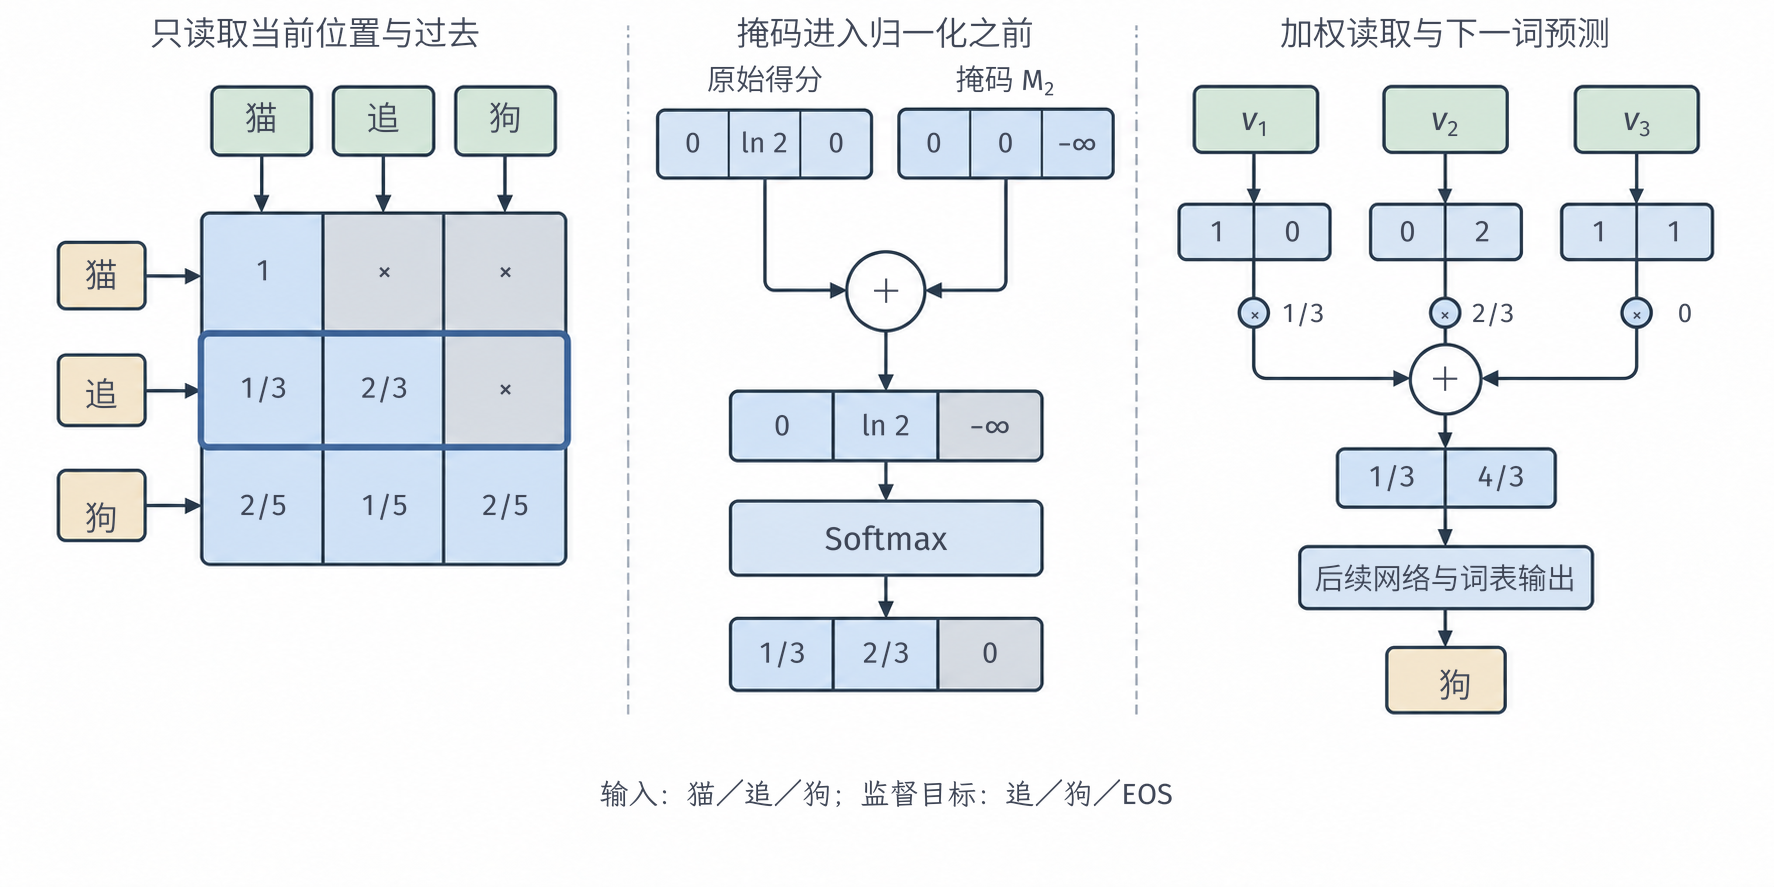
\includegraphics[width=150.199mm]{figures/03-models/02-neural-network-models/generated/transformer-causal-attention/figure.png}
  \caption{“猫／追／狗”的因果自注意力。左图的行对应查询位置，列对应被读取的键；着色格给出可见位置的示例权重，浅灰叉号表示未来位置的权重为0。中图展开“追”这一行：原始得分先加因果掩码，再经Softmax得到$(1/3,2/3,0)$。右图加权读取值，得到$(1/3,4/3)^{\top}$，再经后续网络与词表头形成下一词元的预测分布；图中标出该位置的监督目标“狗”。预测“狗”时只读取当前已经给定的“猫／追”。底部展示错开一步的输入与监督目标，EOS为结束符；数值为教学设定。}
  \label{fig:transformer-causal-attention}
\end{figure*}
\FloatBarrier
\term{填充掩码}（padding mask）阻止有效查询读取填充键；因果掩码排除未来位置。两者可以合并，前者排除不存在的输入，后者排除预测时尚不可知的信息。Softmax要求参与计算的查询至少有一个有效键；全行$-\infty$的指数归一化没有定义。填充查询可以跳过，也可以按有效规则得到随后弃用的输出，以便后续运算保持数值定义。因果掩码允许读取当前输入，这与预测下一个目标的移位配合，才构成没有目标泄漏的生成模型。

\subsubsection{多头注意力：并行形成不同的读取}

单组权重把各值压缩为一个混合。\term{多头注意力}（multi-head attention, MHA）使用$h$组投影分别读取，再把结果拼接：
\begin{equation}
  \begin{aligned}
    \bm Z_a&=\operatorname{Attention}(\bm Q_a,\bm K_a,\bm V_a),\\
    \bm C&=\operatorname{Concat}(\bm Z_1,\ldots,\bm Z_h),\\
    \operatorname{MHA}(\bm H_{\mathrm q},\bm H_{\mathrm s})
      &=\bm C\bm W_{\mathrm o}\text{。}
  \end{aligned}
  \label{eq:transformer-multihead}
\end{equation}
头编号$a\in\{1,\ldots,h\}$，$\bm C\in\mathbb R^{n_q\times hd_v}$，$\bm W_{\mathrm o}\in\mathbb R^{hd_v\times d}$。常取$d_k=d_v=d/h$，使总投影宽度固定。各头分别学习权重和值特征，输出投影再组合这些结果。某头形成什么信息选择，由训练和输入决定；头之间是否互补可以据实际响应检验。固定$d$时增加头数同时减小每头宽度，读取组数与每组特征容量之间形成取舍。

图~\ref{fig:transformer-multihead}展开同一序列上的两个注意力头。三个位置的表示只输入一次，再交给每个头各自的查询、键和值投影；不同的投影使各头能够形成不同的读取权重和值特征。每个头都输出三行向量，拼接时对齐相同位置，只扩展特征维。例如，“追”在两个头中的输出拼为$[\bm z_{2,1}^{\top},\bm z_{2,2}^{\top}]$，这一拼接只扩展当前行的特征维，序列位置数保持原样。输出投影$\bm W_{\mathrm o}$再混合这些特征。多头既可用于自注意力，也可用于交叉注意力；每头还可以施加因果或其他掩码。常见的生成模型因此可以同时采用因果约束、多头投影和自注意力。

\begin{figure*}[p]
  \centering
  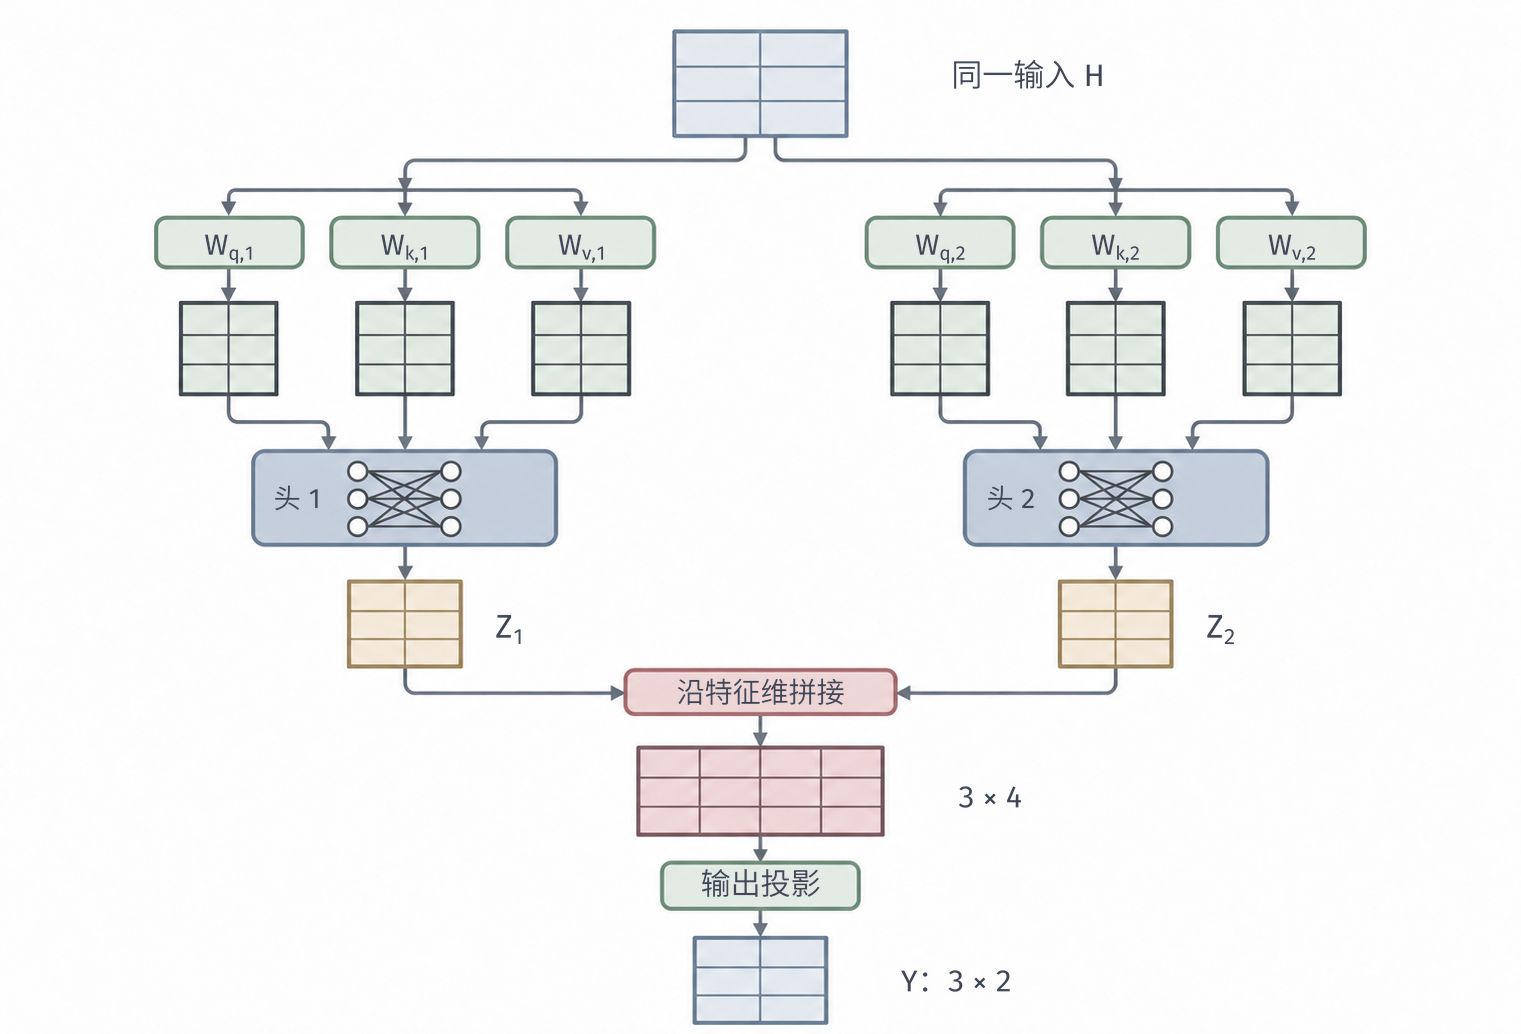
\includegraphics[width=128.778mm]{figures/03-models/02-neural-network-models/generated/transformer-multihead/figure.png}
  \caption{同一输入序列上的两个注意力头。每个头分别学习$\bm W_{\mathrm q,a}$、$\bm W_{\mathrm k,a}$和$\bm W_{\mathrm v,a}$，独立完成评分、归一化和加权聚合，得到$\bm Z_a$。标有“沿特征维拼接”的框合并两路结果，两路输出的序列位置一一对齐，合并只增加特征宽度。拼接矩阵$\bm C$再经$\bm W_{\mathrm o}$投影，得到多头输出$\bm Y$。各头独立形成权重，输出投影组合它们的特征，具体信息分工由训练产生。}
  \label{fig:transformer-multihead}
\end{figure*}
\FloatBarrier

\subsection{前馈层}
\label{sec:transformer-feedforward}

注意力改变每个位置能读取什么，但读取结果还需转换为有用特征。\term{逐位置前馈网络}（position-wise feed-forward network, FFN）对每行单独使用同一组参数，在特征维上扩张、非线性变换，再恢复隐藏宽度：
\begin{equation}
  \operatorname{FFN}(\bm H)
  =\phi(\bm H\bm W_1+\bm 1\bm b_1^{\top})\bm W_2
      +\bm 1\bm b_2^{\top}\text{。}
  \label{eq:transformer-ffn}
\end{equation}
其中$\bm W_1\in\mathbb R^{d\times d_f}$、$\bm W_2\in\mathbb R^{d_f\times d}$，$\bm b_1\in\mathbb R^{d_f}$、$\bm b_2\in\mathbb R^d$；$\bm 1$为$n$维全1向量，$\phi$逐元素作用。原始结构取$d_f=4d$并使用ReLU，其他结构可以采用第\ref{sec:ffn-activations}节介绍的激活函数和不同中间宽度。

每行使用同一FFN，输入内容和上下文不同，输出也随之不同。FFN在这一层不额外交换位置，它把已有上下文中的特征组合成新表示；下一次注意力再依据这些表示进行读取。若去掉非线性，两次仿射映射可以合成一次，扩张宽度本身就失去了增加非线性组合的作用。

这一层的参数量约为$2dd_f$，整段算术量为$O(ndd_f)$。长序列可能由位置对计算主导；短序列且$d_f$很大时，前馈计算和参数占比又会上升。完整成本需要同时计入注意力投影、聚合和前馈变换。

\subsection{残差连接与归一化}
\label{sec:transformer-residual-normalization}

层层变换时，可以让旧表示继续传递，同时学习需要增加的特征。\term{残差连接}（residual connection）把子层输出加到输入上，要求两者形状一致；输入保留一条直接传递路径，子层学习增量。注意力输出投影和FFN的维度恢复，也使这种相加可以在统一的$d$维空间进行。

不同位置的表示尺度还会影响点积和后续激活。\term{层归一化}（layer normalization, LayerNorm）在每个位置内部沿特征坐标计算均值和方差，不依赖其他样本或其他位置的统计量。对$\bm x\in\mathbb R^d$，令
\begin{equation}
  \begin{aligned}
    \mu(\bm x)&=\frac1d\sum_{k=1}^d x_k,\qquad
    s^2(\bm x)=\frac1d\sum_{k=1}^d(x_k-\mu(\bm x))^2,\\
    \operatorname{LN}(\bm x)
      &=\bm\gamma\odot
        \frac{\bm x-\mu(\bm x)\bm 1}{\sqrt{s^2(\bm x)+\varepsilon}}
        +\bm\beta\text{。}
  \end{aligned}
  \label{eq:transformer-layernorm}
\end{equation}
$\bm\gamma,\bm\beta\in\mathbb R^d$为可学习缩放和平移，$\varepsilon>0$避免分母为零，$\odot$表示逐元素乘法。应用于矩阵时按行计算，各位置共享$\bm\gamma,\bm\beta$。均值与方差只来自当前行，位置间模块再按任务掩码读取其他行\scite{ba2016layernorm}

原始Transformer把归一化放在残差相加之后，称为\term{后置层归一化}（post-layer normalization, Post-LN）。一个编码器块为
\begin{equation}
  \begin{aligned}
    \bm U^{(l)}&=\operatorname{LN}_{l,1}\!\left(
       \bm H^{(l-1)}+\operatorname{MHA}_l(\bm H^{(l-1)},\bm H^{(l-1)})\right),\\
    \bm H^{(l)}&=\operatorname{LN}_{l,2}\!\left(
       \bm U^{(l)}+\operatorname{FFN}_l(\bm U^{(l)})\right)\text{。}
  \end{aligned}
  \label{eq:transformer-postln-block}
\end{equation}
实际训练还可在子层输出加入Dropout，预测时关闭；这里省略它以突出确定性结构。\term{前置层归一化}（pre-layer normalization, Pre-LN）先归一化子层输入，再将子层输出加入原表示：
\begin{equation}
  \begin{aligned}
    \bm U^{(l)}&=\bm H^{(l-1)}+
      \operatorname{MHA}_l(\widetilde{\bm H}^{(l-1)},\widetilde{\bm H}^{(l-1)}),\\
    \widetilde{\bm H}^{(l-1)}&=\operatorname{LN}_{l,1}(\bm H^{(l-1)}),\\
    \bm H^{(l)}&=\bm U^{(l)}+
      \operatorname{FFN}_l(\operatorname{LN}_{l,2}(\bm U^{(l)}))\text{。}
  \end{aligned}
  \label{eq:transformer-preln-block}
\end{equation}
Pre-LN通常在整个堆叠末尾再归一化，之后交给输出层。图~\ref{fig:transformer-block}并列展开两种次序：Post-LN在残差相加后归一化，Pre-LN的跳跃路径则绕过归一化和子层；两者的学习性质将在第\ref{sec:transformer-normalization-extensions}节比较。同层各位置复用参数，后续层通常有自己的一组参数；额外的层间共享需要在模型中指定。

\begin{figure*}[htbp]
  \centering
  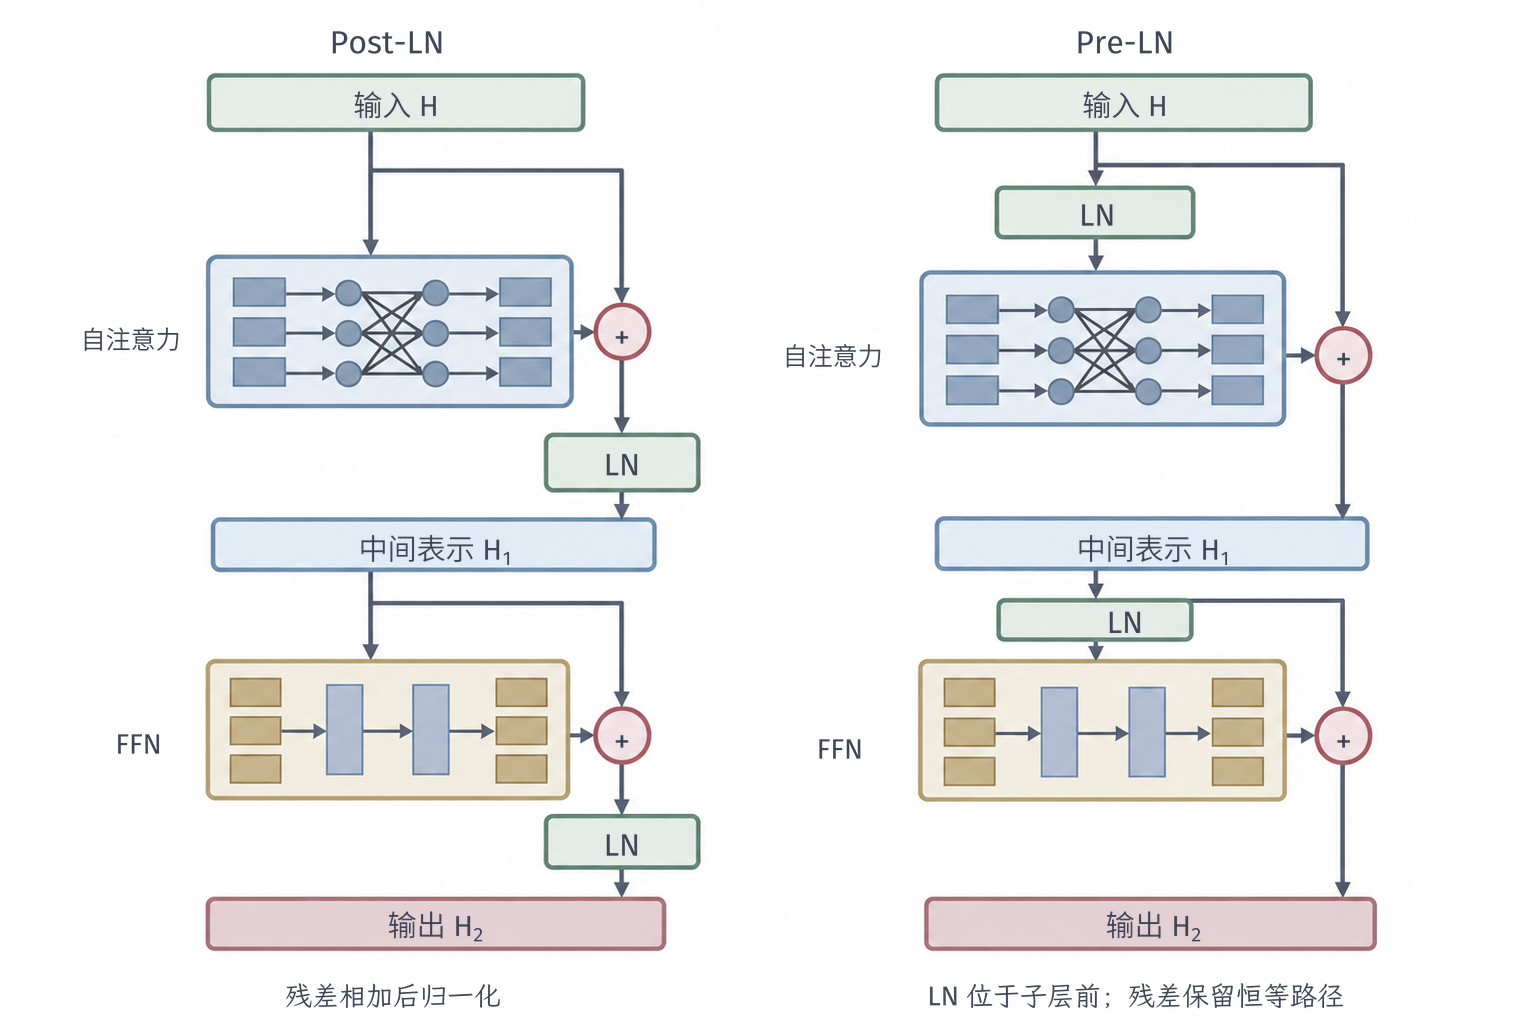
\includegraphics[width=128.778mm]{figures/03-models/02-neural-network-models/generated/transformer-block/figure.png}
  \caption{Post-LN与Pre-LN编码器块的计算次序。输入与输出保持同一序列和特征形状。自注意力在行间交换信息，FFN分别变换各行；圆形$+$表示逐元素残差相加。图中箭头表示前向依赖；从残差路径可见，Post-LN的层间直达路径仍经过LN，Pre-LN则保留绕过归一化和子层的恒等支路。省略Dropout与Pre-LN堆叠末尾的归一化。}
  \label{fig:transformer-block}
\end{figure*}
\FloatBarrier

\subsection{输出和网络架构}
\label{sec:transformer-architectures}

相同网络块可以用于不同预测过程，架构选择取决于输出对应哪些位置，以及这些位置在预测时能读取什么。\term{编码器}（encoder）通常让有效输入位置双向读取，形成整段上下文表示；\term{解码器}（decoder）在生成场景中使用因果自注意力，根据已知前缀预测后续输出。这里的“解码器”既可指原始编码器—解码器中的目标网络，也可指单独使用的因果网络，原始目标网络还读取源表示，单独因果网络则可以只读自身前缀。

\subsubsection{序列到分类或回归}

整段评论分类需要把$n$行表示转为一个向量。若最终输出表示为$\bm H$，有效位置集合为$V$，可以取$\bm r=|V|^{-1}\sum_{i\in V}\bm h_i$，再经分类头计算$\bm p=\operatorname{softmax}(\bm W_{\mathrm c}\bm r+\bm b_{\mathrm c})$。若有$c$类，$\bm W_{\mathrm c}\in\mathbb R^{c\times d}$，目标为$-\log p_y$。回归则用线性或受约束输出头形成数值，并选择与误差含义相符的损失。

另一种方式是在输入中加入专用读出词元，例如CLS，使用其末层表示$\bm r$。专用位置通过注意力读取整段，其输入参数、网络变换和任务头共同学习汇总方式。平均池化显式对位置等权，专用读出位置允许网络学习汇总，两者都要保证只读取任务允许的上下文。

\subsubsection{同步序列到序列}

词性或实体标签与输入位置对齐，可以对每行使用共享分类头，得到$\bm p_i$，在有效监督位置上计算平均交叉熵。离线标注可以读取完整输入；在线预测则需要因果掩码，或明确规定可等待多少后续位置。若预测下一时刻数值，目标还需移位。逐位置标签规定输出与输入的对应；离线、在线或有限延迟条件再规定每个输出可读的范围。

\subsubsection{异步序列到序列}

机器翻译的目标长度和源长度不同。\term{编码器—解码器}（encoder--decoder）先形成源表示$\bm H_{\mathrm s}$，目标网络在每层执行因果自注意力、交叉注意力和FFN。目标查询由该层已有的目标表示产生，键和值由最终源编码表示投影；源端填充掩码与目标端因果掩码分别约束两类读取。图~\ref{fig:transformer-encoder-decoder}中，源表示供每个目标层重复读取，不必随着目标步重新编码。

给定源序列$x$，目标为$y_1,\ldots,y_m$，并将EOS计入目标，则条件分解为
\begin{equation}
  \begin{aligned}
    p_{\bm\theta}(y\mid x)
      &=\prod_{i=1}^{m}p_{\bm\theta}(y_i\mid x,y_{<i}),\\
    \ell(x,y)&=-\frac1m\sum_{i=1}^{m}
          \log p_{\bm\theta}(y_i\mid x,y_{<i})\text{。}
  \end{aligned}
  \label{eq:transformer-conditional-loss}
\end{equation}
$\bm\theta$包含输入、网络块和输出层参数。\term{教师强制}（teacher forcing）在训练时把真实目标前缀送入网络；目标输入是BOS、$y_1,\ldots,y_{m-1}$，目标标签是$y_1,\ldots,y_m$。全段输入已知，各位置可以并行计算，因果掩码保证第$i$个输出没有读到待预测的$y_i$。

条件生成也可用单个解码器：把源输入、分隔符和移位目标组织成同一序列，通常只在目标预测位置计算损失。使用全因果掩码时，源位置也只能读取其前缀；使用前缀掩码时，源位置可互相读取，目标位置可读取全部源前缀和此前目标。两种掩码都能服务于条件生成，源端表示的形成范围却不同。独立编码器—解码器另有源堆栈和交叉读取，三个计算组织应据各自依赖比较。

\begin{figure*}[htbp]
  \centering
  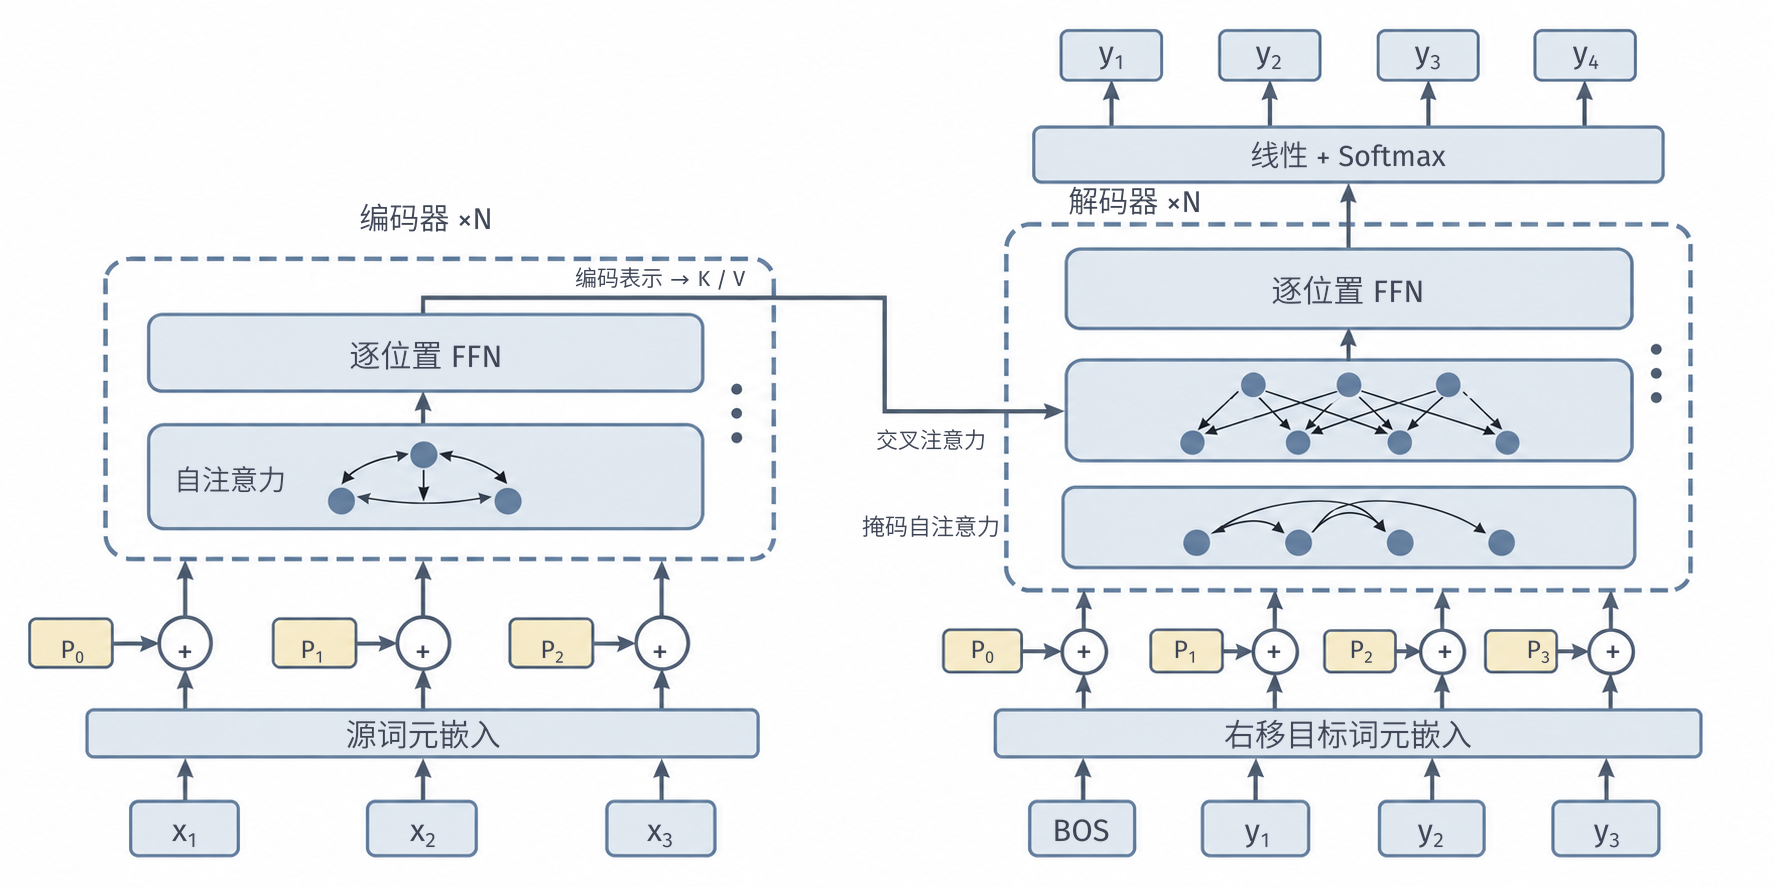
\includegraphics[width=150.199mm]{figures/03-models/02-neural-network-models/generated/transformer-encoder-decoder/figure.png}
  \caption{编码器—解码器的整网依赖结构。每个长条表示作用于整段序列的一层，$\times N$表示重复堆叠；词元列保持位置对应。训练时，目标输入右移后在各目标位置预测对应的下一个词元。左侧最终源表示沿共享读取路径供每个解码器层生成K、V，Q来自该层目标路径；不会把某个中间编码层与同编号解码层一一配对。省略层内残差、归一化与Dropout。}
  \label{fig:transformer-encoder-decoder}
\end{figure*}
\FloatBarrier

\subsubsection{序列续写与生成}

单独的因果解码器省略源交叉注意力，将已有文本本身作为条件。对词元$u_1,\ldots,u_n$，从BOS开始预测时，联合概率为$\prod_{i=1}^n p_{\bm\theta}(u_i\mid u_{<i})$。若最终表示$\bm h_i$对应第$i$个已输入词元，则下一词元概率为
\begin{equation}
  \bm p_{i+1}=\operatorname{softmax}
     (\bm W_{\mathrm{out}}\bm h_i+\bm b_{\mathrm{out}})\text{，}
  \label{eq:transformer-vocabulary-head}
\end{equation}
其中$\bm W_{\mathrm{out}}\in\mathbb R^{v\times d}$。可令$\bm W_{\mathrm{out}}=\bm E$进行输入输出嵌入共享，这使输入取出的内容向量和输出评分共用参数，限制了两接口可以独立调整的自由度。大词表投影还会产生$O(dv)$的单位置计算。

生成从已知前缀开始，计算下一词元分布，按指定策略选择一个词元，将其加入输入，再继续，遇到EOS或最大生成长度停止。贪心每步取当前条件下概率最大的词元，整段概率还随后续条件变化；采样则按指定分布产生词元。训练损失、预测时的选择策略和实际任务评价需分别说明。编码器适合已知完整上下文的理解，因果解码器适合按前缀生成，编码器—解码器使源与目标表示分开组织；输入何时可见与计算预算共同决定这些组织在实际任务中的适用范围。

\subsection{常见Transformer架构}
\label{sec:transformer-common-architectures}

前面按输出形式组织了网络，这里进一步比较几种实际模型。同样面对“猫追狗”，BERT可以补回被遮蔽的“追”，GPT可以根据“猫追”续写“狗”，编码器—解码器则可以把整句翻译成另一种语言。它们共享注意力与前馈计算，但读取范围、监督位置和生成过程不同。以下架构图沿用整序列的分层表示：长条作用于整段序列，虚线框表示重复堆叠，箭头表示前向信息依赖。BERT和RoBERTa另用公式展开一个Post-LN块，GPT则并列比较归一化次序。长条和块内公式分别说明词元读取与层间更新\scite{bishop2024deep} 各图都把中文例子按词划分，以便观察对应关系；这种教学划分不代表某个模型实际采用的子词分词器，图中的词元是监督目标或示例生成结果。

\subsubsection{原始Transformer：源与目标分开建模}

翻译时，源句通常已经完整给定，目标句却需要逐词产生。这两个条件不同，原始Transformer便用两组网络分别处理：编码器双向读取源句，解码器因果读取已有译文，再通过交叉注意力查询源表示。原论文基础模型的编码器和解码器各有6个块，隐藏宽度512，8个注意力头，FFN中间宽度2048，采用正弦位置编码、ReLU与Post-LN\scite{vaswani2017}

以“猫追狗”的翻译说明图~\ref{fig:transformer-architecture-original}的条件生成过程。训练时，解码器输入是右移的目标“BOS、cat、chases、dog”，对应监督目标是“cat、chases、dog、EOS”。预测dog的目标位置可以读取cat和chases，同时通过交叉注意力读取源句中的“狗”；“狗”的源词元属于已经给定的条件，目标词元dog则是这一位置需要预测的监督标签。推理时没有正确译文可供右移，解码器把自己已经生成的词元作为后续输入。

参数学习最小化式\eqref{eq:transformer-conditional-loss}的条件负对数似然，编码器、解码器和词表头一起更新。教师强制允许并行计算所有目标位置，但生成时仍须逐步扩展前缀；训练用真实前缀而预测用自身输出，会使两种过程经历不同的输入分布。源投影和已有目标键值可以缓存，复用先前前向结果；新的目标词元仍在本步选择后进入下一步输入。

这种组织可以一次编码源句，并在多个解码步骤中复用源表示，源端也能充分结合左右语境，适合输入和输出边界明确的翻译、摘要等任务。代价是需要维护两组网络和交叉注意力；当任务只是从一个前缀继续写下去时，单一路径的因果模型通常更直接。成本比较还需固定源长、目标长、宽度和层数，两组堆栈及交叉注意力各占多少计算由这些配置决定。

\begin{figure*}[p]
  \centering
  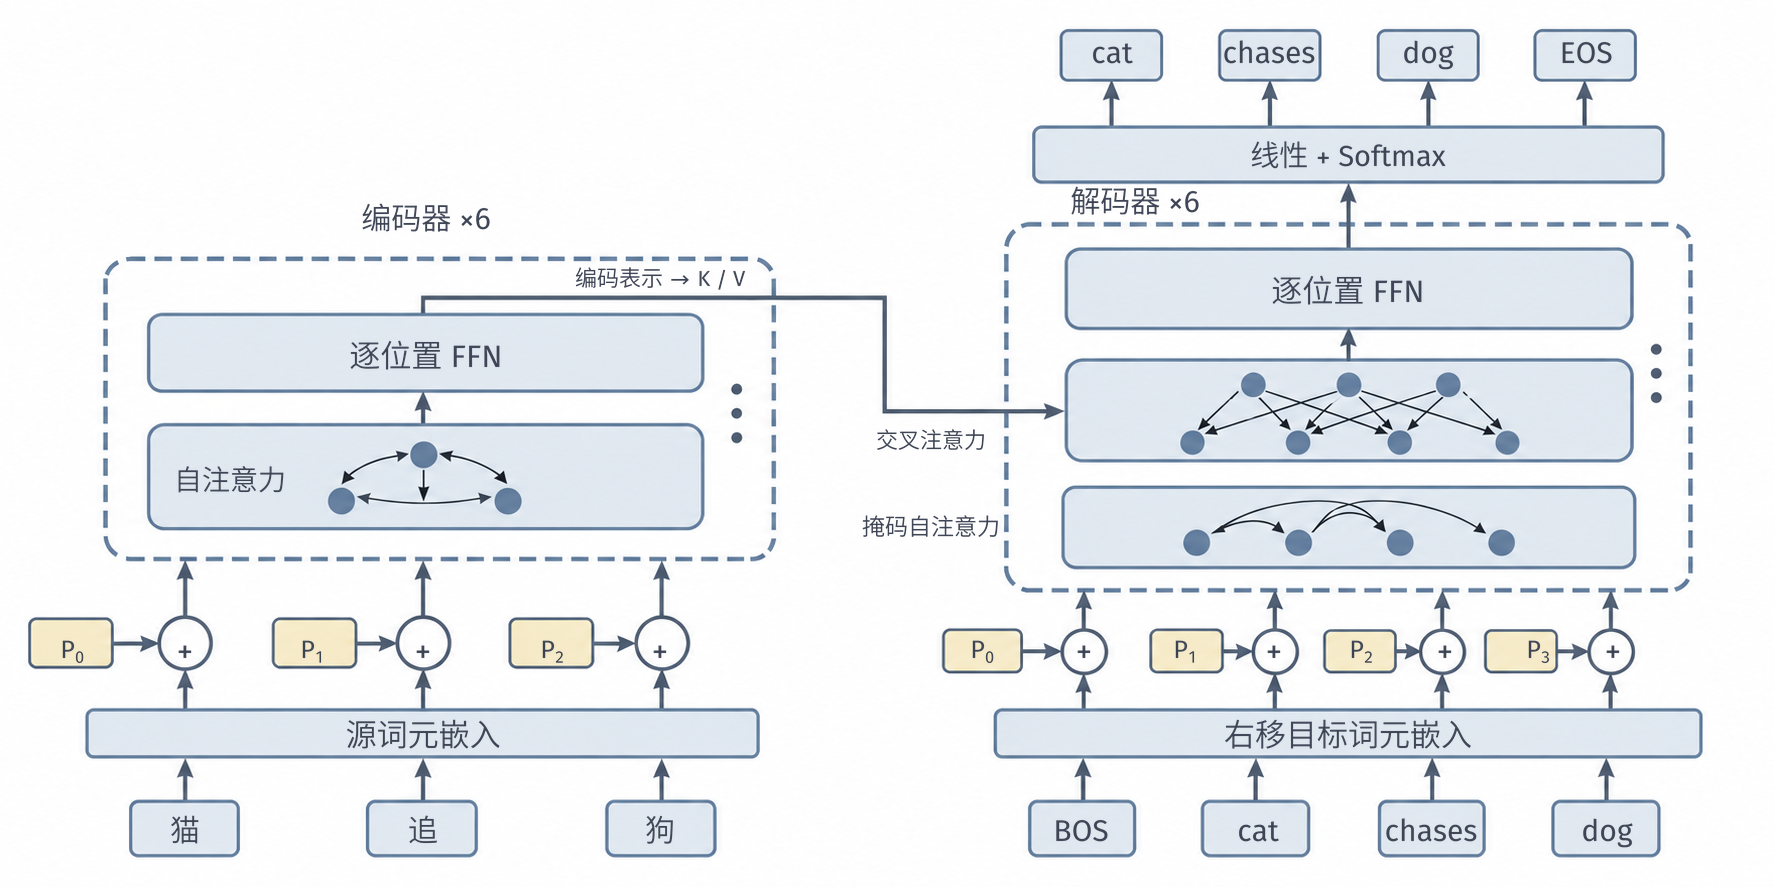
\includegraphics[width=150.199mm]{figures/03-models/02-neural-network-models/generated/transformer-architecture-original/figure.png}
  \caption{原始Transformer基础模型的整网信息流。源编码器与目标解码器各堆叠6个块；每个长条作用于整段序列。解码器先因果读取目标前缀，再交叉读取最终源表示；源表示供各目标块复用。目标输入右移，输出为对应的下一词元，最后预测EOS。省略残差、Post-LN、Dropout和嵌入缩放；结构依据Vaswani等（2017）。}
  \label{fig:transformer-architecture-original}
\end{figure*}
\FloatBarrier

\subsubsection{BERT：利用左右语境形成表示}

若目标是判断句意或标注每个词元，当前位置常常需要后文。\term{BERT}保留双向编码器，并使用\term{遮蔽语言模型}（masked language model, MLM）预训练：先扰动部分输入，再从上下文恢复原词元。例如输入“猫 [MASK] 狗”时，被遮蔽位置必须结合“猫”和“狗”预测“追”。原始BERT还通过CLS位置的表示预测两个句段是否相邻，即下一句预测（next sentence prediction, NSP）。BERT Base为12层、宽度768、12个头，Large版本为24层、宽度1024、16个头；输入叠加词元、可学习位置和句段嵌入，块内使用GELU与Post-LN\scite{devlin2019}

图~\ref{fig:transformer-architecture-bert}中，MLM只在选中的位置接受词元监督；用于分类时，则可以在CLS表示上接任务头。原始训练并非把每个选中位置都替换为[MASK]，还混合随机替换和保留原词，以减轻预训练输入与实际使用输入的差别。这里画出遮蔽分支，是为了突出双向上下文如何帮助恢复缺失内容。

原始BERT随机选取约15%的普通词元作为MLM监督位置，其中80%改为[MASK]、10%替换为随机词元、10%保持原样。设选中集合为$M$、扰动输入为$\widetilde x$，词元损失为$-\sum_{i\in M}\log p_{\bm\theta}(x_i\mid\widetilde x)$；未选位置仍提供上下文，但不直接接受这项恢复监督。原始预训练还加上句段对的二分类损失。微调时换接任务头，使用任务标注继续更新编码器；冻结编码器只训练头则是另一种成本较低的使用方式。

双向读取使BERT适合在完整输入上做分类、抽取和序列标注；各位置表示可以在一次前向计算中并行形成。MLM按扰动输入恢复选中词元，定义了这种条件预测。自由续写还需要左到右或其他序列生成目标及对应解码过程。若当前位置读取了未经扰动的自身内容，恢复同一词元便有直接答案可用，因而目标和可见输入必须一起设计。

\begin{figure*}[p]
  \centering
  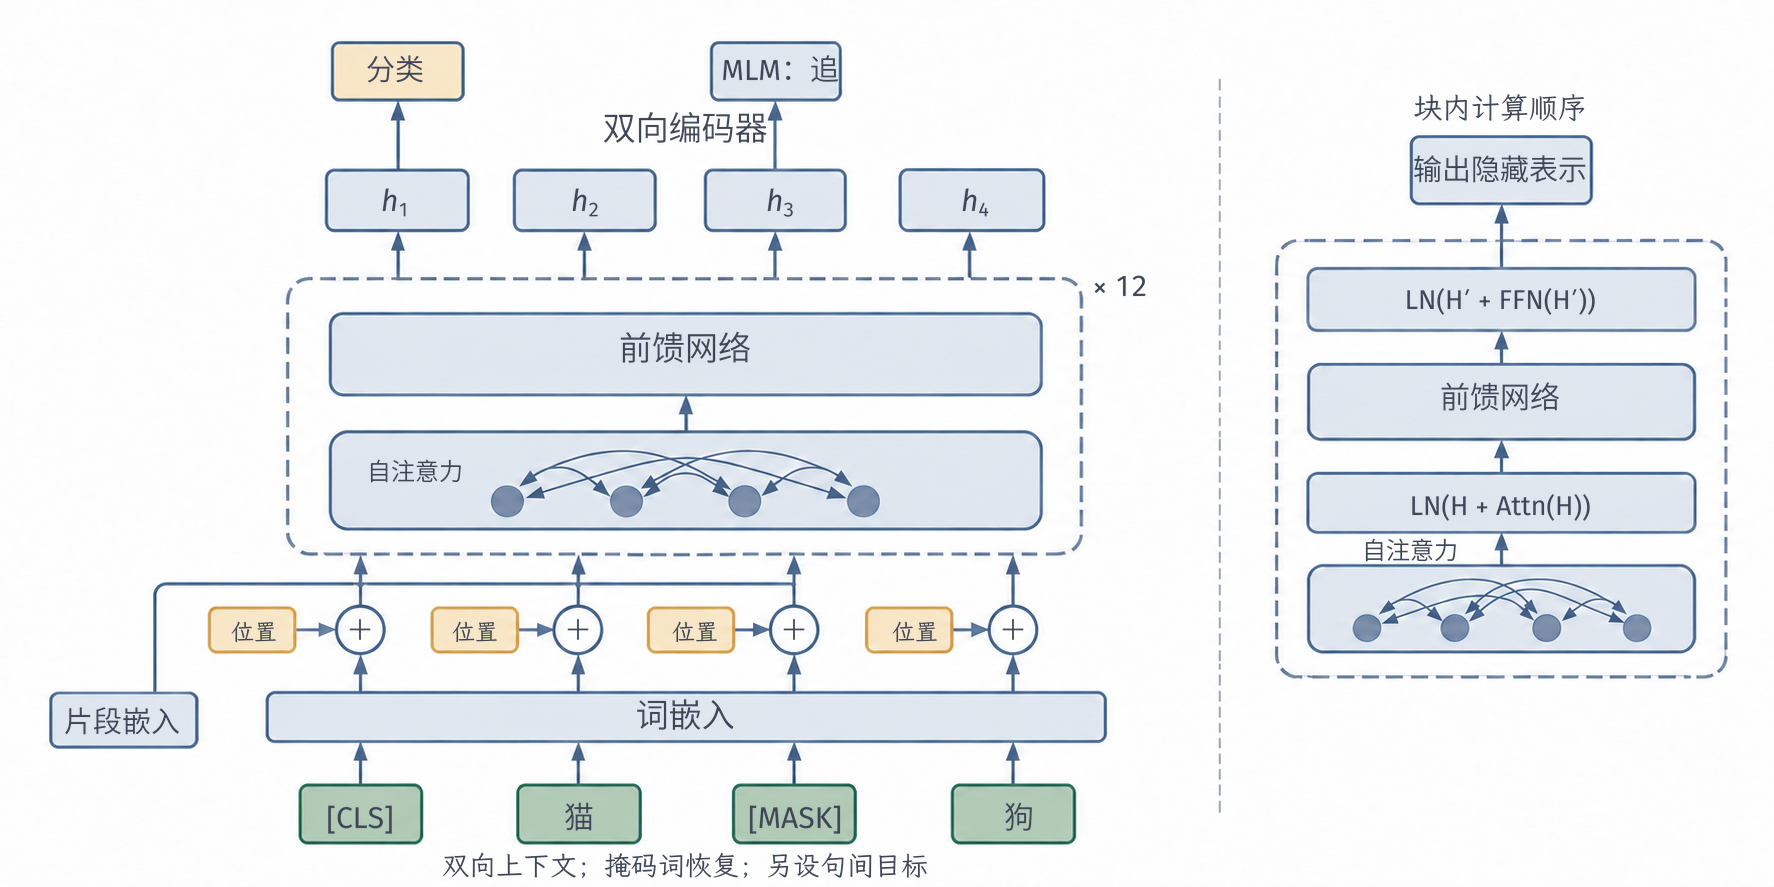
\includegraphics[width=150.199mm]{figures/03-models/02-neural-network-models/generated/transformer-architecture-bert/figure.png}
  \caption{BERT Base的双向编码器与预测位置。词元、位置和句段嵌入相加，12个编码器块形成上下文表示；左侧画出一个短片段，省略分隔符。CLS用于序列分类，遮蔽位置由MLM头恢复“追”。主流程省略层内残差与归一化，右侧展开一个Post-LN块；$\operatorname{Attn}$、$\operatorname{FFN}$分别表示注意力与前馈变换，$\bm H'$表示注意力子层残差归一化后的输出。残差直接写入公式；省略Dropout与NSP头。结构依据Devlin等（2019）。}
  \label{fig:transformer-architecture-bert}
\end{figure*}
\FloatBarrier

\subsubsection{RoBERTa：改进双向编码器的预训练}

BERT的效果还取决于预训练方式，而不仅是网络拓扑。\term{RoBERTa}保留BERT式双向编码器，主要改变训练配方：每次送入序列时重新抽取遮蔽位置，取消NSP，使用更大的批次、更多文本和更充分的训练，并改用字节级BPE词表。图~\ref{fig:transformer-architecture-roberta}沿用BERT式编码器，画出遮蔽“追”的一次训练输入；动态遮蔽表示不同次训练可以重新抽取遮蔽位置，让模型接触不同的上下文恢复问题\scite{liu2019roberta}

它仍在选中的位置计算MLM交叉熵，不同遮蔽样本通过同一网络分别前向；各样本内部双向读取，样本之间不交换词元。NSP是句段级训练目标，取消它改变了样本组织和损失；编码器内部的注意力模块保持原来的读取作用。下游分类或标注仍需把末层表示接到相应任务头，并明确哪些参数继续训练。

RoBERTa以相同核心结构检验数据、目标与优化设置的作用。其预训练投入和方案同时变化，论文的整体收益应结合这些配置解释；单项改动的作用需要相应对照实验。两者在使用方式上仍然接近，都适合完整输入上的理解任务，也都需要额外设计才能作为自由续写模型。

\begin{figure*}[p]
  \centering
  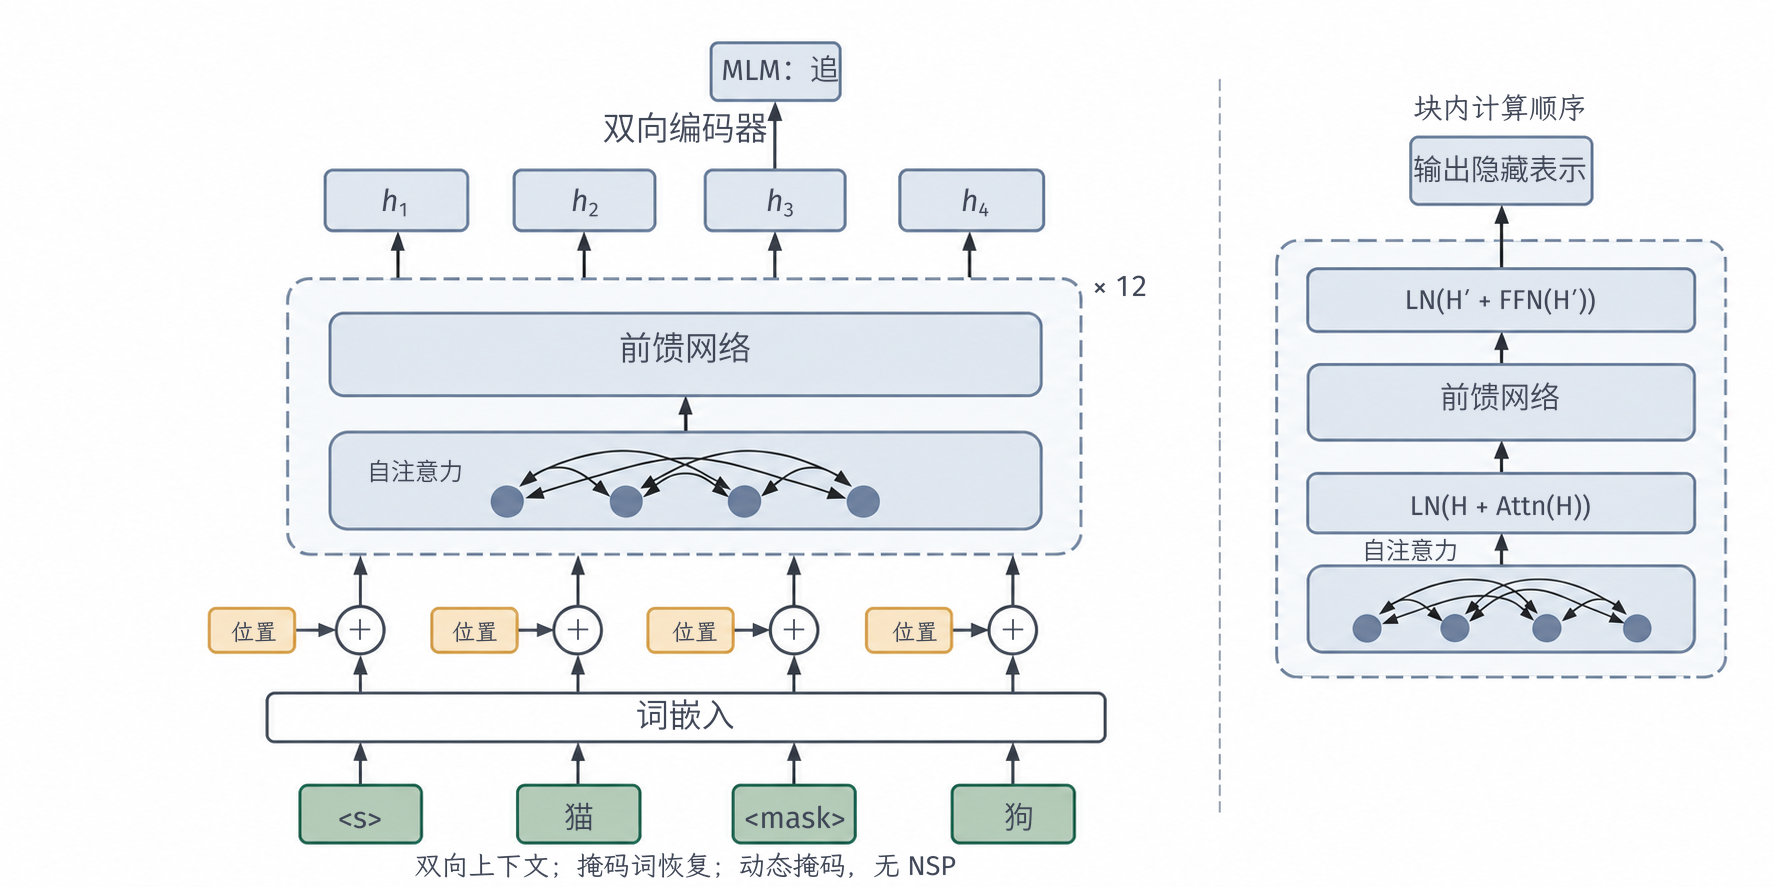
\includegraphics[width=150.199mm]{figures/03-models/02-neural-network-models/generated/transformer-architecture-roberta/figure.png}
  \caption{RoBERTa Base的双向编码器与遮蔽恢复。词元与可学习位置嵌入相加，12个编码器块形成上下文表示，选中的遮蔽位置由MLM头恢复“追”。核心结构与BERT相同，预训练采用动态遮蔽且不使用NSP。主流程省略层内残差与归一化，右侧展开Post-LN计算次序；省略Dropout。训练差异依据Liu等（2019）。}
  \label{fig:transformer-architecture-roberta}
\end{figure*}
\FloatBarrier

\subsubsection{GPT：因果解码器及其版本演进}

续写时，模型只能依据已经出现的内容预测下一项。\term{GPT}家族由这一任务发展而来；早期公开的GPT-1、GPT-2和GPT-3都采用只有解码器的组织，每个块包含因果自注意力与FFN，没有独立源编码器，也没有连接源表示的交叉注意力。版本演进涉及块内计算、模型规模、训练目标和使用方式，以下分别说明它们改变的输入与参数。

\paragraph{GPT-1：建立预训练后微调的因果模型}

初代GPT于2018年采用12层、宽度768、12个头的结构，配合可学习绝对位置、GELU与Post-LN；先用下一词元预测进行语言模型预训练，再针对下游任务微调。为便于与后续版本区分，这里称其为GPT-1\scite{radford2018gpt}

图~\ref{fig:transformer-architecture-gpt}并列比较早期三个版本的计算次序。以词元序列说明监督：“猫”位置预测“追”，“追”位置预测“狗”。训练时三个位置可以一起计算，因为因果掩码已经阻止了未来信息进入各层表示；推理时则必须先选出“追”，才能把“猫追”作为下一步的前缀。把问题、示例或文档放在前缀中，后面接答案，就能沿同一条路径完成条件生成。

\begin{figure*}[p]
  \centering
  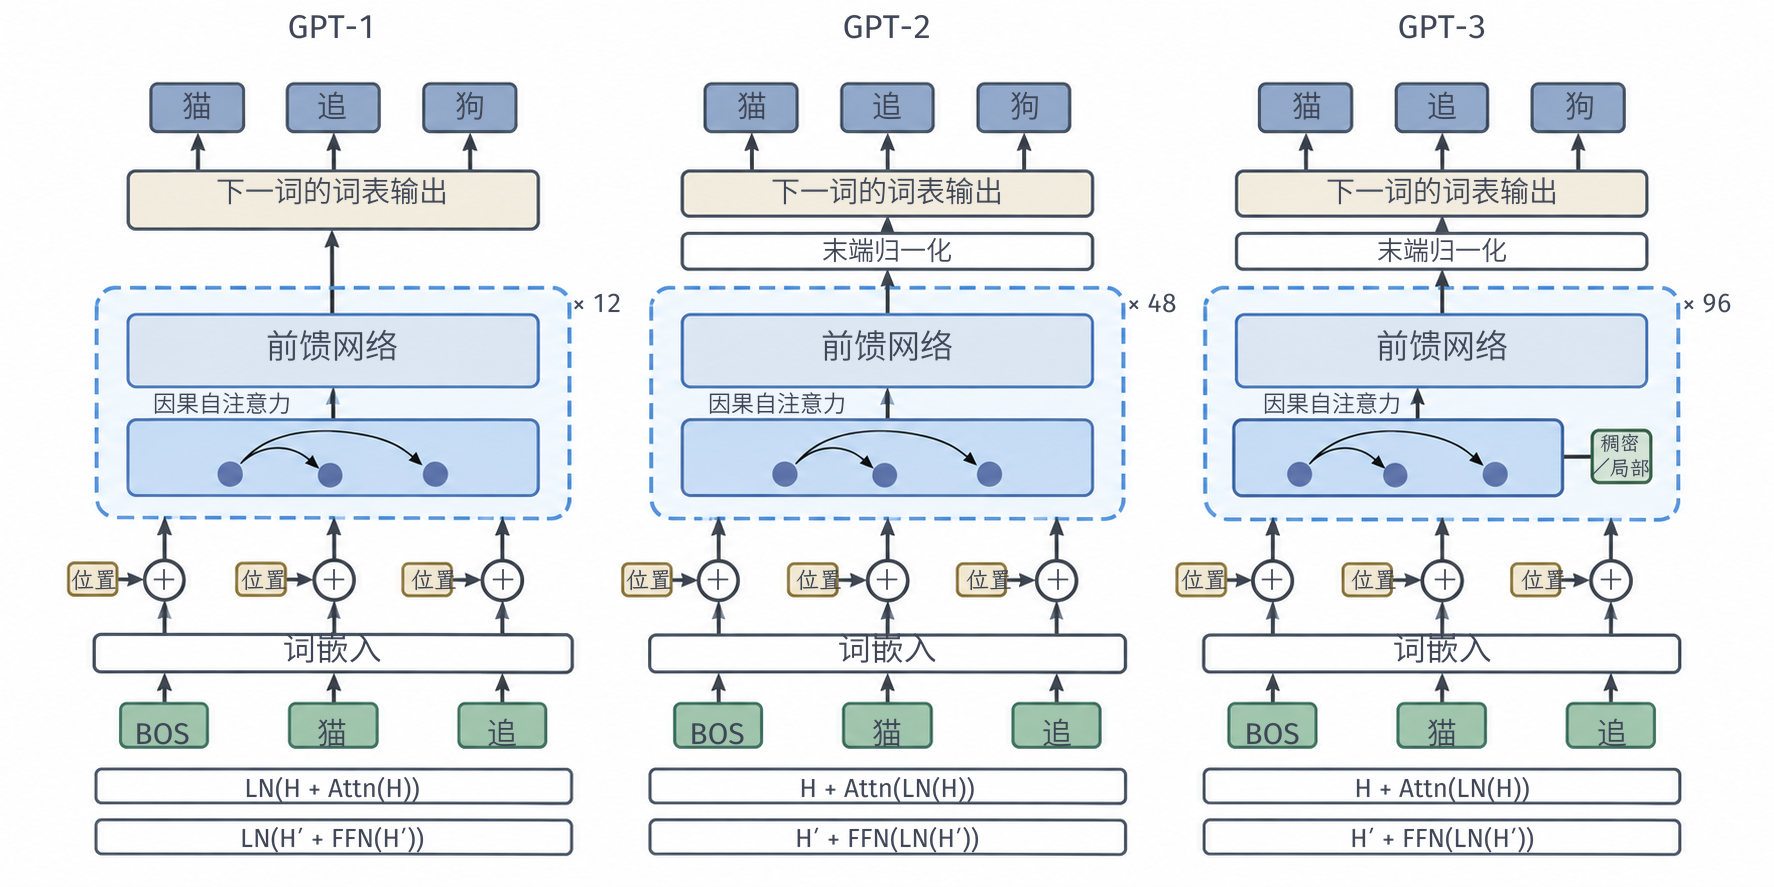
\includegraphics[width=150.199mm]{figures/03-models/02-neural-network-models/generated/transformer-architecture-gpt/figure.png}
  \caption{GPT-1、GPT-2与GPT-3的公开块结构对比。各列下方的公式包括子层变换、残差和归一化；各版本中的$\operatorname{Attn}$均遵守因果约束。GPT-1采用Post-LN，GPT-2和GPT-3采用Pre-LN并增加堆叠末端归一化；GPT-3还交替使用稠密与局部带状注意力。层数指各原论文的最大公开配置，省略Dropout、内部投影和KV缓存；比较依据相应原论文。}
  \label{fig:transformer-architecture-gpt}
\end{figure*}
\FloatBarrier

这条因果路径使训练目标与逐词生成直接对应，条件和输出可以采用统一的文本接口。早期位置的表示只使用当时前缀，BERT的词元表示则可结合后文；两类表示服务于不同可见条件。长输出还要依次建立新的前缀。用于分类时，因果模型可以在读完整段后的末位置作判断，也可以生成类别名称，但这与BERT在CLS上使用固定类别头的损失和输出空间不同。

\paragraph{GPT-2：调整归一化位置并扩大模型}

GPT-2保留因果解码器，将归一化从子层残差相加之后移到子层入口，形成Pre-LN，并在整个堆栈末端增加归一化。这样的变化修改了深层残差路径中的计算顺序，具体梯度差异可结合第\ref{sec:transformer-residual-normalization}节理解。GPT-2还扩大模型和网页训练语料，进一步考察不更新参数时的零样本迁移。原论文最大配置为48层、宽度1600、约15亿参数，上下文长度由GPT-1的512提高到1024\scite{radford2019gpt2}

% GPT-3论文的全作者边注较长，需在本段之前保留竖向空间。
\Needspace{190mm}
\paragraph{GPT-3：扩大规模并交替使用两种注意力连接}

GPT-3沿用GPT-2的总体组织与Pre-LN，但在不同层中交替采用稠密和局部带状稀疏注意力。前者允许当前位置读取全部已有前缀，后者只保留规定的局部连接；两者都遵守因果约束。最大的公开配置为96层、宽度12288、96个头、1750亿参数，上下文长度2048。论文系统研究了\term{上下文学习}，即把少量任务示例放入前缀，而不在该任务的推理阶段更新模型参数\scite{brown2020}

这一步同时涉及网络与使用方式：增加层数和宽度扩大了可学习参数，调整注意力连接改变了每层的信息路径，而在提示中提供示例改变的是当前输入。上下文学习通过当前提示提供任务信息，微调通过梯度改变模型参数；两者可以改变预测，却在不同对象上起作用。

% 为InstructGPT论文的全作者边注保留竖向空间。
\Needspace{165mm}
\paragraph{InstructGPT与GPT-3.5阶段：让生成服从指令和对话}

续写目标奖励文本中的下一词元，人类指令任务还要求输出符合请求与偏好。InstructGPT在语言模型基础上加入人类示范的监督微调，再用人类偏好训练奖励模型并优化输出，使训练目标更贴近指令遵循\scite{ouyang2022instructgpt}2022年发布的ChatGPT则基于GPT-3.5系列模型进行了面向对话的微调。GPT-3.5是模型系列名称，ChatGPT是对话系统名称；这项演进说明基础训练之后的参数调整与对话交互；具体内部拓扑需要对应的架构材料才能确定\scite{openai2022chatgpt}

\paragraph{GPT-4与GPT-4o：扩展输入输出模态}

GPT-4的技术报告公开了图像与文本输入、文本输出，以及下一词元预训练和人类反馈后训练等信息，但明确未披露模型规模和详细内部架构。GPT-4o则进一步公开了文本、视觉与音频的端到端联合训练。这些公开材料支持比较模态、训练目标及接口能力；层数、专家数量与位置编码等内部细节则保留为未披露信息\scite{openai2023gpt4,openai2024gpt4o}

\paragraph{GPT-5发布系统：在模型之间选择计算路径}

2025年GPT-5发布时，官方将其在ChatGPT中的形态描述为一个统一系统：路由器在快速响应模型与更深入的推理模型之间选择。这里的路由器选择的是整个模型；后文的混合专家模型（MoE）则在一个网络层内，为各词元选择少量计算分支。系统路由选择整条模型路径，层内路由选择词元计算分支；发布说明只支持前一种组织的描述，各模型的内部配置仍需单独披露\scite{openai2025gpt5}

图~\ref{fig:transformer-gpt-public-interfaces}进一步比较后续版本公开的接口和系统层次。灰色模块表示内部结构未完整披露；GPT-5发布系统的两条模型路径是系统级选择，它展示发布系统的选择流程，每个内部模型的专家组织留待相应资料说明。

\begin{figure*}[p]
  \centering
  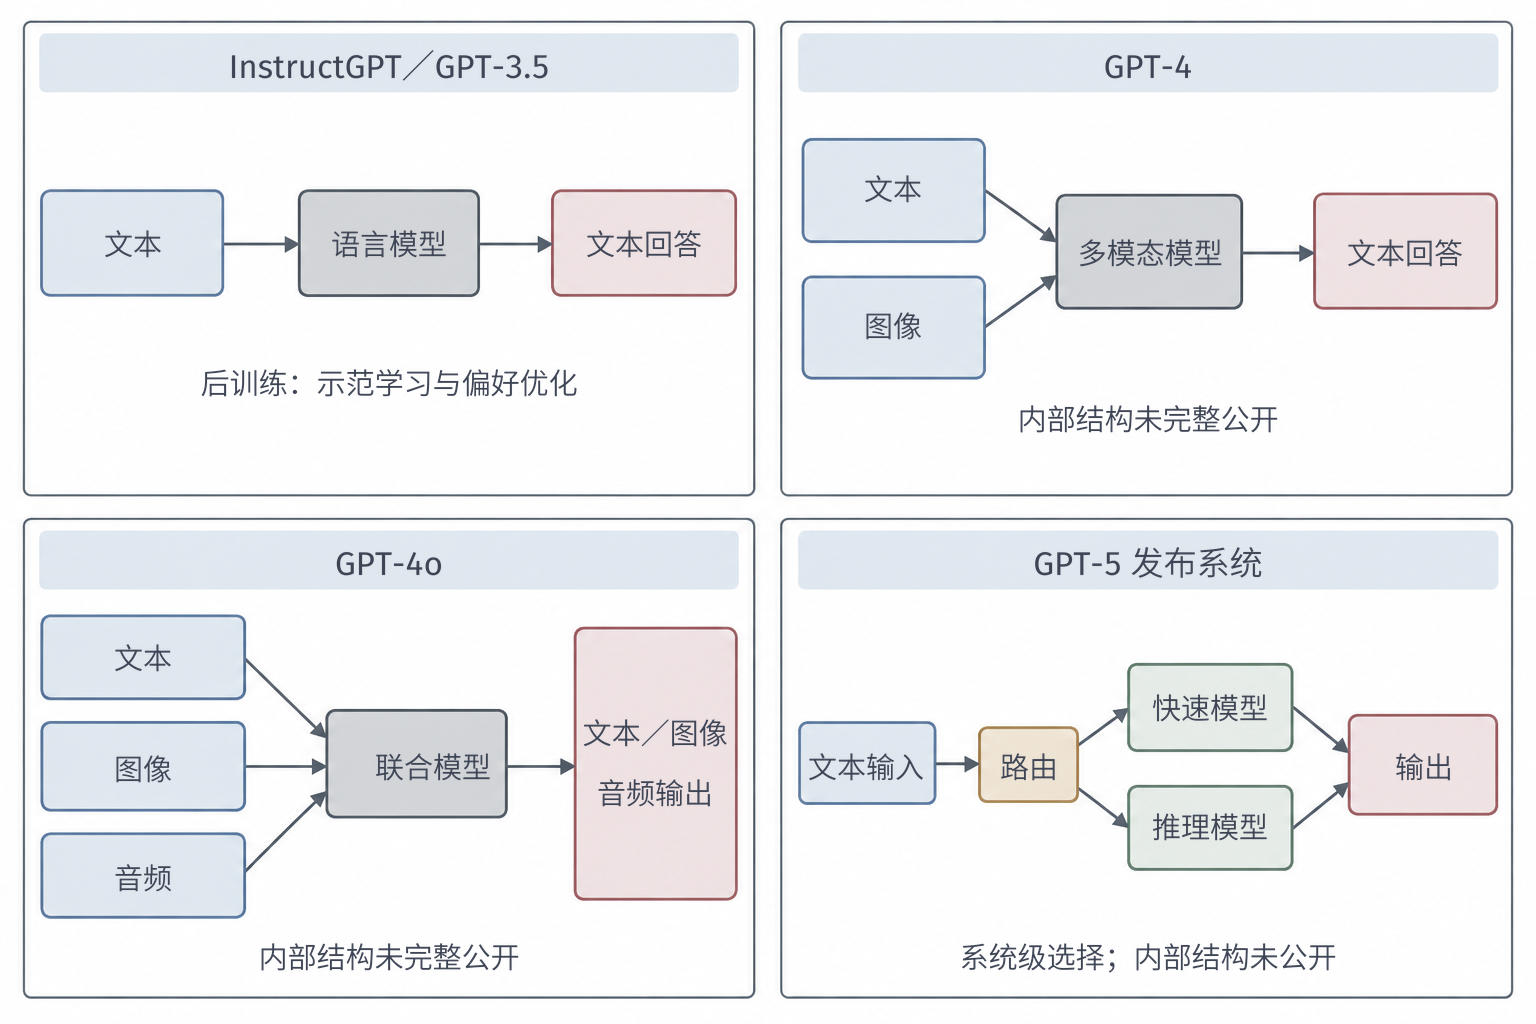
\includegraphics[width=130.048mm]{figures/03-models/02-neural-network-models/generated/transformer-gpt-public-interfaces/figure.png}
  \caption{GPT后续代表版本的公开接口与系统组织。InstructGPT／GPT-3.5阶段主要改变后训练和交互；GPT-4支持图像与文本输入、文本输出；GPT-4o以文本、视觉、音频端到端联合训练，图示对应模型能力，特定产品功能以各发布阶段的实际开放范围为准；GPT-5发布系统在快速与深入推理模型间路由。灰色模块标明尚未披露的逐层细节，绿色模块仅标示所公开的计算路径。信息依据对应官方报告与发布说明，版本比较截至图中标注的发布阶段。}
  \label{fig:transformer-gpt-public-interfaces}
\end{figure*}
\FloatBarrier

表~\ref{tab:transformer-gpt-generations}将各代变化对应到已经披露的对象。GPT-1至GPT-3可以比较具体块结构与配置；后续公开材料更多描述后训练、模态和系统组织，能够支持的比较也相应有所不同。

\begin{table*}[p]
  \centering
  \small
  \begin{tabular}{@{}p{25mm}p{64mm}p{66mm}@{}}
    \toprule
    代表版本 & 已公开的主要变化 & 阅读这些变化时应保留的区别 \\
    \midrule
    GPT-1（2018） & 因果解码器、Post-LN；12层、宽768；语言模型预训练后进行任务微调 & 预训练目标与下游任务监督可以不同 \\
    GPT-2（2019） & 改用Pre-LN并增加末端归一化；最大约15亿参数；1024词元上下文 & 零样本任务提示不需要再训练一个专用输出头 \\
    GPT-3（2020） & 延续Pre-LN；稠密与局部稀疏注意力交替；最大1750亿参数；2048词元上下文 & 提示中的少样本示例不等于梯度微调 \\
    InstructGPT／GPT-3.5阶段（2022） & 人类示范与偏好用于后训练；ChatGPT采用对话交互 & 基座模型、后训练方法和对话产品分属不同层面 \\
    GPT-4（2023） & 图像与文本输入，生成文本；内部架构细节未公开 & 多模态能力不提供确定参数量或专家数的证据 \\
    GPT-4o（2024） & 文本、视觉、音频端到端联合训练 & 模态扩展不能直接还原为一张已知的逐层网络图 \\
    GPT-5发布系统（2025） & 在快速响应与深入推理模型之间路由 & 系统级模型选择不等于层内词元级MoE \\
    \bottomrule
  \end{tabular}
  \caption{GPT家族的代表性演进。参数与上下文数字指相应原论文的配置，GPT-4之后列出官方明确披露的能力或系统组织，不推测未公开的网络细节；表格也不用于比较当前产品的可用性。}
  \label{tab:transformer-gpt-generations}
\end{table*}
\FloatBarrier

\subsubsection{T5：把不同任务组织成文本到文本}

翻译生成另一种语言，分类输出一个类别，摘要输出较短文本；这些任务可以共享“读入条件文本、生成目标文本”的接口。\term{T5}（Text-to-Text Transfer Transformer）使用编码器—解码器，把任务说明和输入交给双向编码器，由因果解码器生成答案并交叉读取条件。它保留原始Transformer的两条路径，但采用相对位置偏置、Pre-LN和简化的归一化；原始基础FFN使用ReLU\scite{raffel2020t5}

T5的代表预训练任务是恢复被删去的连续片段。图~\ref{fig:transformer-architecture-t5}把“猫追狗”变成“猫$\langle S_1\rangle$狗”，解码器生成“$\langle S_1\rangle$追$\langle S_2\rangle$”，并以EOS结束生成。这些专用标记称为\term{哨兵词元}（sentinel token），作用是标明缺失片段及其边界。一个标记可以代替多个连续词元，因此目标长度可以变化。BERT在选中的输入位置恢复词元，T5在目标端串联缺失片段，逐步生成整段恢复内容。

恢复目标由被删片段及哨兵标记串联而成，保留的源词元作为条件供解码器读取。给定扰动源句，按式\eqref{eq:transformer-conditional-loss}对恢复序列逐词计算损失；教师强制与因果掩码仍然适用。多处缺失按各哨兵的顺序组织，源长、缺失片段总长和标记数共同决定计算量。其Pre-LN仅按均方根调整尺度，保留可学习缩放，省去均值减除和平移项；本章标准LayerNorm另有这两项操作。

这种接口使分类也能写成生成类别文本，任务之间不必各自规定一种输出头；源端双向理解与目标端因果生成的职责保持清楚。相应代价是仍要维护编码器、解码器与交叉注意力，生成式分类还需要规定合法类别词及其读出方式。任务可以复用文本输入输出的训练流程，所需目标长度、合法答案集合和评价量仍由各任务规定。

\begin{figure*}[p]
  \centering
  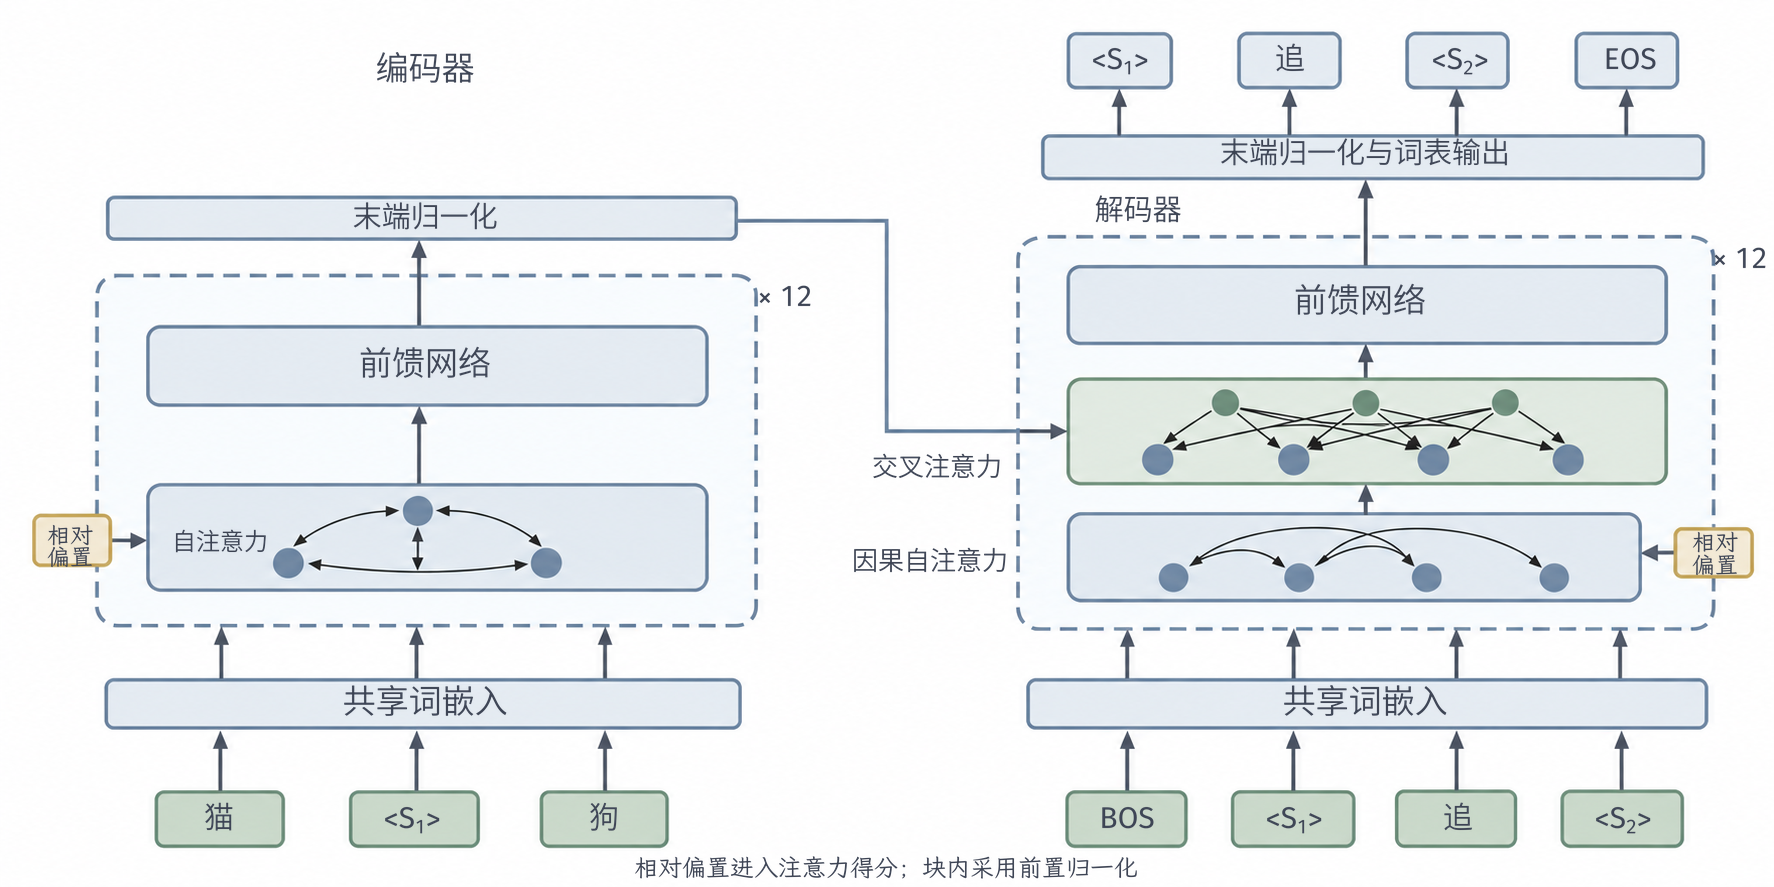
\includegraphics[width=150.199mm]{figures/03-models/02-neural-network-models/generated/transformer-architecture-t5/figure.png}
  \caption{T5 Base的片段恢复与整网结构。$\langle S_1\rangle$替代源句中的缺失片段，目标中的同名标记引出恢复内容，$\langle S_2\rangle$结束该恢复片段，EOS结束生成。BOS表示解码起始输入。编码器与解码器各堆叠12个块，最终源表示供交叉注意力读取。相对位置偏置加入注意力得分，输入不叠加绝对位置向量。图中显式保留堆叠末端归一化，目标端与词表头合并展示；省略块内入口归一化、残差与Dropout。结构和任务依据Raffel等（2020）。}
  \label{fig:transformer-architecture-t5}
\end{figure*}
\FloatBarrier

\subsubsection{架构之间如何取舍}

表~\ref{tab:transformer-common-architectures}将比较标准固定为已知条件、输出过程与结构代价。对一个具体任务，先判断后文何时可见、结果是否需要逐步生成，再选择网络组织。BERT与RoBERTa的主要差异位于预训练方案；原始Transformer与T5共享编码器—解码器组织，却采用不同的位置表示、归一化和任务目标。模型名称还包含训练方案与配置，信息流类型则按允许读取的来源与次序比较。

\begin{table*}[htbp]
  \centering
  \small
  \begin{tabular}{@{}p{24mm}p{34mm}p{47mm}p{50mm}@{}}
    \toprule
    代表模型 & 条件与读取规则 & 结构带来的便利 & 相应代价或使用边界 \\
    \midrule
    原始Transformer & 源双向；目标因果并交叉读取源 & 完整编码源句，生成时复用源表示 & 两组网络和交叉注意力；目标仍逐步产生 \\
    BERT & 扰动输入内双向读取 & 一次形成利用左右语境的各位置表示 & MLM不直接定义自由续写；任务需要适配输出头 \\
    RoBERTa & 与BERT同属双向编码 & 保持结构，改进预训练数据与优化方案 & 预训练投入增大；生成边界与BERT相似 \\
    GPT & 单一路径因果读取 & 前缀与答案共享接口，直接学习逐词生成 & 早期位置不读后文；长输出需要多步解码 \\
    T5 & 条件双向；目标因果并交叉读取条件 & 文本到文本接口统一多种任务 & 双堆栈成本；类别文本等仍需规定读出规则 \\
    \bottomrule
  \end{tabular}
  \caption{代表架构的优势与边界。比较的是信息流和任务接口，不是在不同参数量、训练数据与硬件下比较实测速度或任务分数。同一家族的后续版本还可能修改位置编码、归一化和前馈层。}
  \label{tab:transformer-common-architectures}
\end{table*}
\FloatBarrier

架构规定了可计算的信息路径，训练数据决定模型见过什么，学习目标决定哪些行为受到奖励，解码与系统组织决定模型怎样被调用。这些因素共同构成实际预测过程，各项差异按输入、参数更新和执行步骤分别解释。


\section{参数学习}
\label{sec:transformer-learning}

嵌入、注意力投影、前馈层、归一化和输出层由同一预测目标联合学习。一个批次中的样本可以具有不同有效长度，损失只覆盖监督位置；按样本平均与按词元平均会给予长序列不同权重，相应权重规定了经验目标与后续风险分析中的样本贡献。本节重点说明尺度设置和注意力求导，优化器、学习率调度及通用正则化由训练与泛化章节展开。

\subsection{参数初始化}
\label{sec:transformer-initialization}

第\ref{sec:ffn-initialization}节的对称性打破和方差传播原则仍然适用，但Transformer还需同时控制内容嵌入、点积得分与残差流的尺度。输入嵌入可从零均值分布初始化，不同词元独立采样；如果内容项使用$\sqrt d$缩放，初始方差应连同这一缩放考虑。可学习位置表也需要适当尺度，避免输入在尚未学习时被位置项完全主导。连续输入则应先明确量纲和训练数据归一化，再设置投影。

对不带激活的投影$\bm Y=\bm X\bm W$，若输入坐标零均值、方差为$s_x^2$，各权重彼此独立、与输入独立、零均值且方差为$s_w^2$，输入宽度为$d_{\mathrm{in}}$，简化计算给出输出坐标方差$d_{\mathrm{in}}s_w^2s_x^2$。可用Glorot尺度兼顾输入输出宽度，或用与$d_{\mathrm{in}}^{-1}$同阶的方差控制前向尺度；ReLU前馈支路则可采用式\eqref{eq:ffn-he-initialization}的思路。激活、门控和残差参数化会继续改变尺度，投影方差因此按各支路的输入与输出配置。

查询与键的初始尺度直接影响Softmax。若二者每坐标方差分别为$s_q^2,s_k^2$，沿用坐标独立和零均值近似，缩放后点积方差为$s_q^2s_k^2$。因此，除以$\sqrt{d_k}$只抵消宽度因素；过大的投影范数仍会使得分过尖。值与输出投影则决定注意力支路加入残差的大小。FFN的第二次投影也位于残差支路末端，应与第一投影和非线性一起检查输出尺度。

深度增加时，多次相加可能持续放大残差流。若一个简化子层写为$\bm h^{(l)}=\bm h^{(l-1)}+a_l\bm f^{(l)}$，且各增量与已有表示不相关、各坐标方差为$s_f^2$，则增量方差之和为$\sum_l a_l^2s_f^2$。取$a_l$与$L^{-1/2}$同阶可在这个近似下控制累积量；实际分支往往相关，深层训练还需联合考察这些相关性、梯度和归一化位置。缩小支路末端权重、显式残差缩放与可学习门控是不同参数化，后文会比较它们怎样控制新增支路。

归一化的缩放和平移常分别初始化为1和0；输出层按其输入宽度设置尺度。若输入输出共享嵌入，两处梯度会累积到同一参数，初始化也只执行一次。把整个投影都置零可能阻断上游学习：例如$\bm Q=\bm K=\bm0$时，得分对查询和键的局部梯度都为零。特定设计也会把少量支路末端置零。此时可沿计算图确定初始哪些参数有非零导数，以及后续更新怎样打开这些路径。

\subsection{反向传播}
\label{sec:transformer-backpropagation}

注意力的参数既影响“读取什么”，也影响“怎样评分”。为把两条路径分清，采用矩阵梯度记号$\bm G_{\mathrm X}=\partial\ell/\partial\bm X$，其形状与$\bm X$相同，并以Frobenius内积定义微分$\mathrm d\ell=\langle\bm G_{\mathrm X},\mathrm d\bm X\rangle_{\mathrm F}$。从式\eqref{eq:transformer-attention}中单头的$\bm Z=\bm A\bm V$开始，若下游给出$\bm G_{\mathrm Z}$，则
\begin{equation}
  \bm G_{\mathrm V}=\bm A^{\top}\bm G_{\mathrm Z},\qquad
  \bm G_{\mathrm A}=\bm G_{\mathrm Z}\bm V^{\top}\text{。}
  \label{eq:transformer-aggregation-gradient}
\end{equation}
值梯度汇集所有查询对同一值的读取贡献；权重梯度比较不同值对当前输出变化的作用。固定权重时仍有值梯度；学习读取比例时，还要从权重沿Softmax和评分继续回传。

对第$i$行，把有效权重写为列向量$\bm a_i$。Softmax各权重由共同分母耦合，将其Jacobian与该行权重梯度相乘，得到
\begin{equation}
  (\bm G_{\mathrm S})_{i,j}
   =\bm A_{i,j}\left((\bm G_{\mathrm A})_{i,j}
       -\sum_{t=1}^{n_s}\bm A_{i,t}(\bm G_{\mathrm A})_{i,t}\right)\text{。}
  \label{eq:transformer-softmax-gradient}
\end{equation}
这一求导使用Softmax的局部Jacobian（参考\BookEquationRef{eq:analysis-softmax-jacobian}{第一卷“数学准备”的softmax Jacobian公式}）。计算限定在有效集合上，被禁止的权重与得分梯度取零，以避免把无穷掩码当作普通浮点变量求导。每行得分梯度之和为零，与Softmax对整行得分加同一常数不变的性质对应。Softmax的共同分母让各权重相互影响：某个值的梯度要减去当前加权平均作用，才得到该位置的得分梯度。

\Needspace{45mm}
\begin{example}[从聚合误差到评分误差]
  \label{ex:transformer-gradient-numerical}
  沿用示例~\ref{ex:transformer-attention-numerical}未加掩码的情形，令$\ell=(\bm z_2)_2$，即只考察“追”的输出向量的第二坐标，上游梯度为$(0,1)^{\top}$。三个权重的梯度为$0,2,1$，加权平均为$5/4$，得分梯度因此为$-5/16,3/8,-1/16$，总和为零。值梯度则分别为$(0,1/4)^{\top}$、$(0,1/2)^{\top}$和$(0,1/4)^{\top}$。若最小化此目标，评分路径倾向于降低第二个值的权重，值路径还可以直接降低被读取的第二坐标；两种变化共同影响输出。
\end{example}

掩码固定时，对缩放点积继续求导可得
\begin{equation}
  \bm G_{\mathrm Q}=\frac{\bm G_{\mathrm S}\bm K}{\sqrt{d_k}},\qquad
  \bm G_{\mathrm K}=\frac{\bm G_{\mathrm S}^{\top}\bm Q}{\sqrt{d_k}}\text{。}
  \label{eq:transformer-qk-gradient}
\end{equation}
查询梯度聚合相关键，键梯度聚合读取它的查询；固定因果掩码只删除禁止的贡献。若得分还包含可学习位置偏置，相应参数按其使用的所有位置对累积得分梯度。

式\eqref{eq:transformer-qkv}的投影梯度为
\begin{equation}
  \begin{aligned}
    \nabla_{\bm W_{\mathrm q}}\ell&=\bm H_{\mathrm q}^{\top}\bm G_{\mathrm Q},\\
    \nabla_{\bm W_{\mathrm k}}\ell&=\bm H_{\mathrm s}^{\top}\bm G_{\mathrm K},\qquad
    \nabla_{\bm W_{\mathrm v}}\ell=\bm H_{\mathrm s}^{\top}\bm G_{\mathrm V},\\
    \bm G_{\mathrm H_{\mathrm q}}&=\bm G_{\mathrm Q}\bm W_{\mathrm q}^{\top},\\
    \bm G_{\mathrm H_{\mathrm s}}&=\bm G_{\mathrm K}\bm W_{\mathrm k}^{\top}
                      +\bm G_{\mathrm V}\bm W_{\mathrm v}^{\top}\text{。}
  \end{aligned}
  \label{eq:transformer-projection-gradient}
\end{equation}
交叉注意力的两侧接到不同上游模块；自注意力的两侧是同一矩阵，所以查询、键、值三条输入梯度需要相加。加入投影偏置时，其梯度为对应矩阵梯度沿位置求和。共享词元嵌入也按词元编号把各出现位置的贡献相加。

多头输出若为$\bm Y=\bm C\bm W_{\mathrm o}$，则$\nabla_{\bm W_{\mathrm o}}\ell=\bm C^{\top}\bm G_{\mathrm Y}$，$\bm G_{\mathrm C}=\bm G_{\mathrm Y}\bm W_{\mathrm o}^{\top}$。按拼接的列范围拆开$\bm G_{\mathrm C}$，各头分别执行上述求导，再将共同输入的梯度求和。各头分别更新自己的投影，共同输入则接收所有读取分支的梯度和。

残差相加把同一上游梯度送入直接路径和子层路径。对Pre-LN子层$\bm y=\bm x+F(\operatorname{LN}(\bm x))$，列向量记号下有
\begin{equation}
  \bm g_{\mathrm x}=\bm g_{\mathrm y}
     +\bm J_{\operatorname{LN}}^{\top}\bm J_F^{\top}\bm g_{\mathrm y}\text{。}
  \label{eq:transformer-preln-gradient}
\end{equation}
FFN沿用前馈求导，LN在一行内部耦合坐标。若归一化输出为$\bm y$，令$\widehat{\bm x}=(\bm x-\mu\bm1)/\sqrt{s^2+\varepsilon}$、$\bm u=\bm g_{\mathrm y}\odot\bm\gamma$，以横线表示坐标平均，则
\begin{equation}
  \bm g_{\mathrm x}
   =\frac{\bm u-\overline u\bm1
             -\widehat{\bm x}\,\overline{u\widehat x}}
          {\sqrt{s^2+\varepsilon}}\text{。}
  \label{eq:transformer-layernorm-gradient}
\end{equation}
缩放和平移的梯度分别由$\bm g_{\mathrm y}\odot\widehat{\bm x}$和$\bm g_{\mathrm y}$沿位置、样本累积。训练中若使用Dropout，还需按前向使用的同一随机掩码回传。至此，输出损失可以经注意力的读取与评分、逐位置变换和残差路径，传到全部可训练参数；梯度提供参数更新方向，优化进展还取决于目标形状、步长及所用梯度估计。

\section{Transformer的扩展}
\label{sec:transformer-extensions}

标准网络将输入表示、位置读取、特征变换和残差更新组合起来。扩展方法可以改变其中某个计算，也可以只改变同一计算的执行与存储方式。位置关系决定怎样匹配，特征选择决定哪些读取结果进入更新；位置对运算、中间激活及生成缓存又分别消耗计算和存储。扩展方法按这些具体目标调整不同部分。这些目标会影响不同资源，因而可以组合，也可能相互制约。

\subsection{位置编码的扩展}
\label{sec:transformer-position-extensions}

顺序信息可以加到输入，也可以进入位置对评分。前者给每个位置一个表示，后者让读取直接依赖相对距离；旋转则提供了把位置变换嵌入点积的实现机制。下面固定内容投影，比较位置到底在哪里参与计算。

\subsubsection{绝对位置编码}

可学习位置表$\bm P\in\mathbb R^{n_{\max}\times d}$直接提供式\eqref{eq:transformer-input-position}中的$\bm p_i$，参数量为$n_{\max}d$。位置表只覆盖设定上限，扩充或插值提供新位置向量后，新增长度上的预测还需训练支持或相应外推检验。固定正弦编码对偶数宽度$d$定义
\begin{equation}
  \begin{aligned}
    (\bm p_i)_{2k+1}&=\sin(i\omega_k),\\
    (\bm p_i)_{2k+2}&=\cos(i\omega_k),\qquad
    \omega_k=10000^{-2k/d},
  \end{aligned}
  \label{eq:transformer-sinusoidal-position}
\end{equation}
其中$k=0,\ldots,d/2-1$，向量坐标从1开始，$i$采用本章从1开始的位置编号；改从0开始时需统一输入约定。不同频率使坐标随位置以不同速度变化，无需学习位置表，任意整数位置都可以求值。

图~\ref{fig:transformer-position-waves}把这个变化画成波形。为在同一位置区间内看清快慢，这里取$d=8$，只画$k=0,1$对应的前四个坐标：两对角频率分别为1和0.1弧度／位置。它与图~\ref{fig:transformer-position-example}的四维手算例采用相同公式，但宽度不同；四维例子的第二对频率是0.01，不能把两组参数混用。每对正弦与余弦具有相同周期，彼此相差四分之一周期；高频坐标随位置较快振荡，低频坐标变化较慢。同一横坐标处的各维幅值一起构成该位置向量，每条曲线只提供一个坐标。

\begin{figure}[htbp]
  \centering
  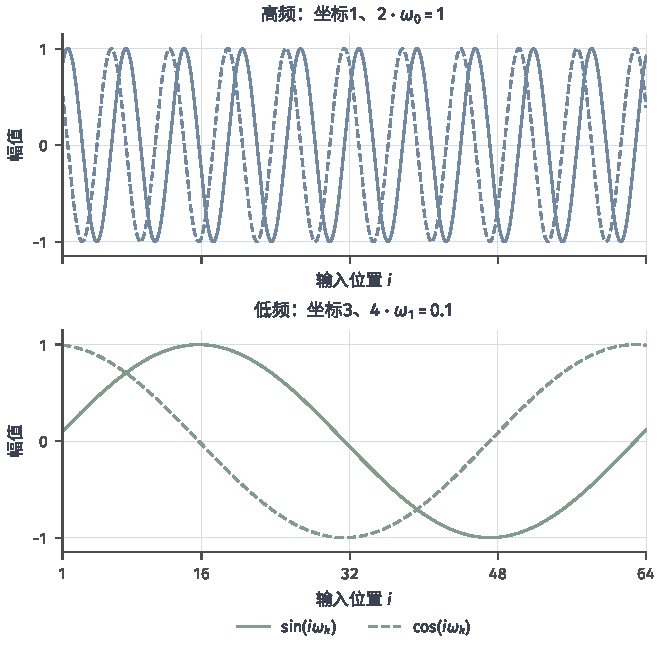
\includegraphics[width=105.412mm]{figures/03-models/02-neural-network-models/matplotlib/transformer-position-waves/figure.pdf}
  \caption{固定正弦编码中选定坐标随输入位置的变化。取$d=8$，上图为坐标1、2（$k=0$），下图为坐标3、4（$k=1$）；两图横轴范围相同，幅值无量纲。实线为正弦，虚线为同频余弦，周期分别约为6.28和62.83个位置。连续曲线帮助观察波形，实际序列只在整数位置取值；本图仅示意选定维度，不是完整八维编码或训练结果。}
  \label{fig:transformer-position-waves}
\end{figure}
\FloatBarrier

对固定距离$\Delta$，加法公式把$\bm p_{i+\Delta}$写为$\bm p_i$各坐标对的线性变换。这一变换给出位置位移的规律。完整注意力还处理内容投影，所以其得分可以同时依赖内容与位置。把内容和位置相加后，投影点积还包含内容与位置的交叉项；网络需要学习如何使用这些项。新位置向量可以直接求值；训练长度外的预测质量还取决于新上下文与距离如何进入已学计算。

\subsubsection{相对位置向量与距离偏置}

若任务更关心“相隔多远”而非“位于第几位”，可以直接让位置对得分依赖$j-i$。\term{相对位置编码}（relative positional encoding）为位置之间的关系提供表示。设$\bm r_{j-i}^{\mathrm k}\in\mathbb R^{d_k}$、$\bm r_{j-i}^{\mathrm v}\in\mathbb R^{d_v}$为距离对应的键和值修正，则一种形式为
\begin{equation}
  \begin{aligned}
    S_{i,j}&=\frac{\bm q_i^{\top}(\bm k_j+\bm r_{j-i}^{\mathrm k})}
                        {\sqrt{d_k}}+M_{i,j},\\
    \bm z_i&=\sum_j A_{i,j}(\bm v_j+\bm r_{j-i}^{\mathrm v})\text{。}
  \end{aligned}
  \label{eq:transformer-relative-position}
\end{equation}
这里$S_{i,j},M_{i,j},A_{i,j}$是对应矩阵元素的简写，$\bm q_i,\bm k_j,\bm v_j$是各行转置后的向量。键修正改变匹配，值修正把距离信息带入输出。Shaw等采用截断距离，共享过远位置的相对向量；这样限制参数数量，也合并了某些距离差异\scite{shaw2018relative}

若只需修改评分，可以使用标量偏置$b_{j-i}$，将其加到缩放点积上。偏置表可按距离截断或分桶，后者让一组距离共享参数；同一距离只存一个标量时，参数比同距离向量少；它调整评分，向量修正还可以改变匹配方向或输出内容。\term{线性偏置注意力}（attention with linear biases, ALiBi）在因果读取中采用
\begin{equation}
  S_{i,j}^{(a)}=\frac{\bm q_{i,a}^{\top}\bm k_{j,a}}{\sqrt{d_k}}
                 -m_a(i-j),\qquad j\leq i\text{，}
  \label{eq:transformer-alibi}
\end{equation}
其中$m_a>0$是第$a$头的预设斜率，未来位置仍由掩码排除。距离越远，扣除越多；不同斜率提供不同距离偏好。它无需训练长度对应的位置表，原论文在特定语言建模设置中检验了长度外推。这个结果依赖模型、数据与长度范围，线性距离偏好也可能不符合需要精确远距离访问的任务\scite{press2021alibi}

回到“猫／追／狗”，图~\ref{fig:transformer-position-extensions}把相对位置写成可逐格检查的距离矩阵。“追”读取“狗”对应$j-i=1$；若整段句子在更长文本中同时后移5位，距离仍为$8-7=1$。ALiBi进一步把距离变成得分修正：图中“狗”读取三个位置时分别扣除$1.0,0.5,0$，之后才做Softmax。图~\ref{fig:transformer-position-example}是在输入上相加，而这里是在每一对位置的评分上相加，两个操作作用于不同对象。

\begin{figure*}[htbp]
  \centering
  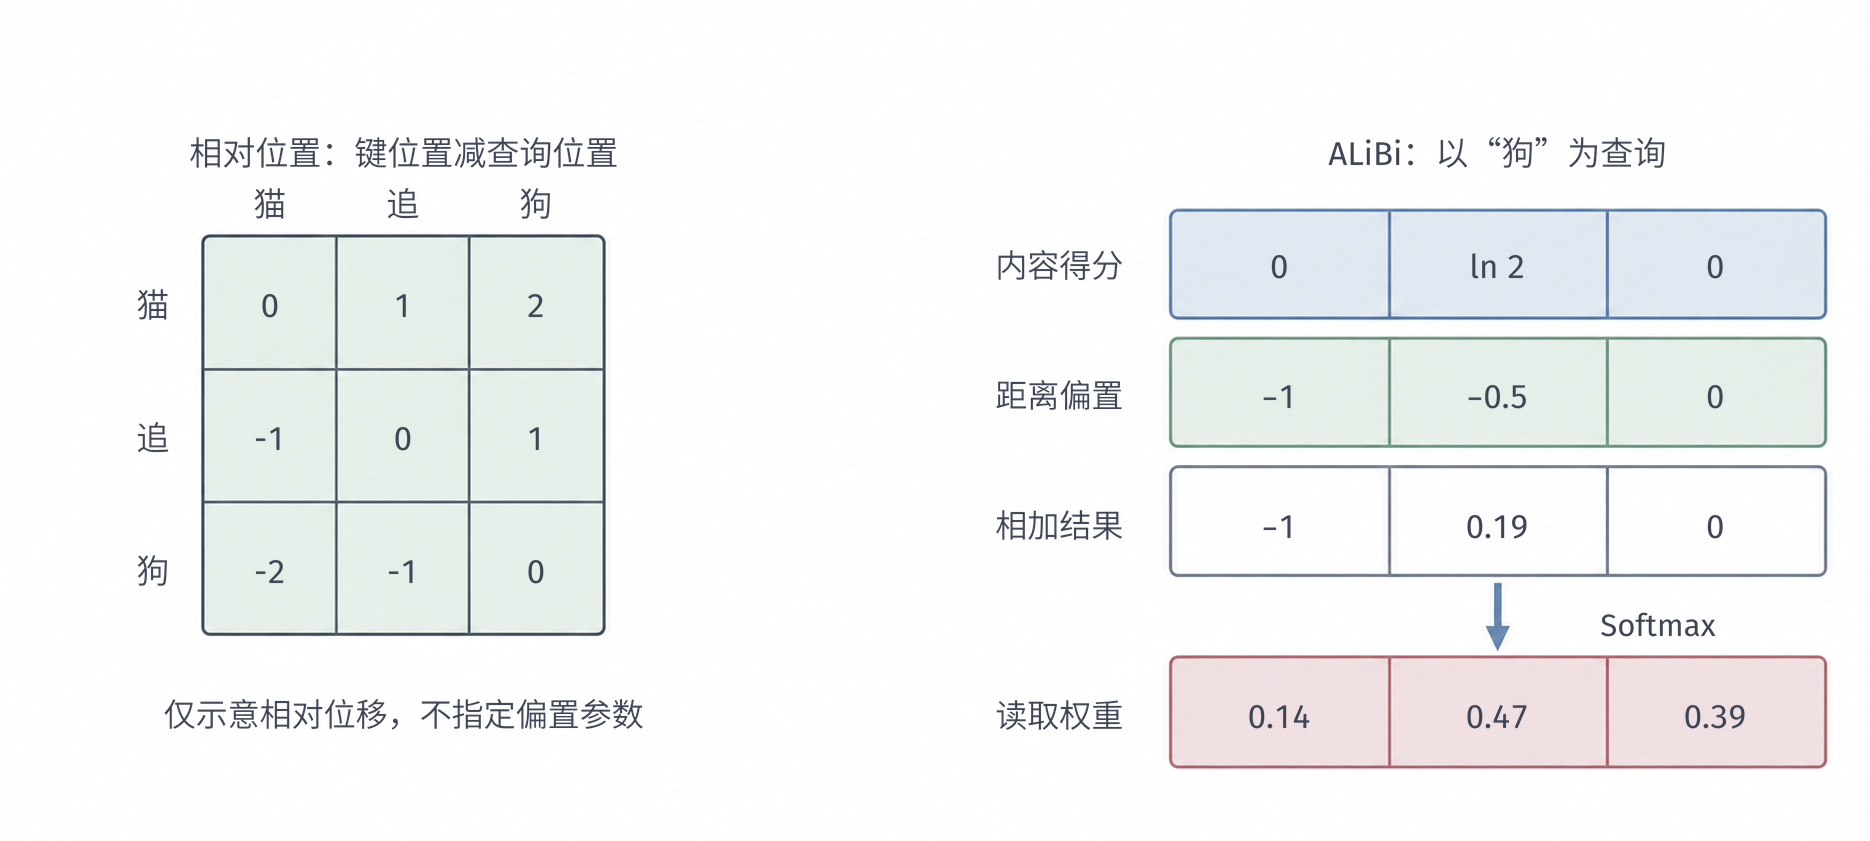
\includegraphics[width=158.327mm]{figures/03-models/02-neural-network-models/generated/transformer-position-extensions/figure.png}
  \caption{“猫／追／狗”的相对位置。左图行是查询位置$i$、列是键位置$j$，格内为$j-i$，正负号区分左右方向。右图取“狗”为查询、斜率$m=0.5$，演示ALiBi如何修正教学得分并重新归一化；显示数值保留两位小数，真实计算使用未舍入值。}
  \label{fig:transformer-position-extensions}
\end{figure*}
\FloatBarrier

\subsubsection{旋转位置编码}

查询与键怎样变换，决定位置如何进入它们的点积。绝对向量相加会引入内容与位置的交叉项；另一种构造直接控制位置对关系：分别根据位置$i$、$j$变换查询和键，但要求变换后的点积只通过$j-i$依赖位置。\term{旋转位置编码}（rotary position embedding, RoPE）用旋转实现这一要求：位置决定旋转角度，两向量的相对角度进入点积\scite{su2021roformer}

\paragraph{为什么旋转能表示位移}
先考虑二维向量。希望位置每增加1，就施加同一个变换，而且连续移动$i$步再移动$j$步，应等价于移动$i+j$步。平面旋转满足这种组合规律，还能保留向量长度。设每步旋转$\omega$弧度；单位横轴旋转$\theta$后变为$(\cos\theta,\sin\theta)^{\top}$，单位纵轴变为$(-\sin\theta,\cos\theta)^{\top}$。把它们作为两列，就得到
\begin{equation}
  \bm R(\theta)=
  \begin{pmatrix}
    \cos\theta&-\sin\theta\\
    \sin\theta&\cos\theta
  \end{pmatrix}\text{。}
  \label{eq:transformer-rope-rotation}
\end{equation}
对尚未施加本层RoPE旋转的查询$\bm q_i=(q_{i,1},q_{i,2})^{\top}$，令
\[
  \widetilde{\bm q}_i=\bm R(i\omega)\bm q_i
  =\begin{pmatrix}
     q_{i,1}\cos(i\omega)-q_{i,2}\sin(i\omega)\\
     q_{i,1}\sin(i\omega)+q_{i,2}\cos(i\omega)
   \end{pmatrix}\text{；}
\]
键同样取$\widetilde{\bm k}_j=\bm R(j\omega)\bm k_j$。这里旋转的是投影后的查询和键，内容向量仍决定旋转前的方向和长度。

\paragraph{从两个绝对角度推到相对位置}
矩阵转置把旋转角取反。再利用三角函数的和角公式，逐项相乘可得
\begin{equation}
  \begin{aligned}
    \bm R(\alpha)^{\top}&=\bm R(-\alpha),\\
    \bm R(\alpha)\bm R(\beta)&=\bm R(\alpha+\beta),\\
    \bm R(i\omega)^{\top}\bm R(j\omega)
      &=\bm R((j-i)\omega)\text{。}
  \end{aligned}
  \label{eq:transformer-rope-composition}
\end{equation}
令$\Delta=j-i$，代入两向量的点积，有
\begin{equation}
  \begin{aligned}
    \widetilde{\bm q}_i^{\top}\widetilde{\bm k}_j
      &=\bm q_i^{\top}\bm R(\Delta\omega)\bm k_j\\
      &=(q_{i,1}k_{j,1}+q_{i,2}k_{j,2})\cos(\Delta\omega)\\
      &\quad +(q_{i,2}k_{j,1}-q_{i,1}k_{j,2})\sin(\Delta\omega)\text{。}
  \end{aligned}
  \label{eq:transformer-rope-two-dimensional}
\end{equation}
两个内容乘积组合分别乘上余弦和正弦，位置只以$\Delta$出现。若保持内容向量固定，把$i$和$j$同时加上$c$，差值不变，点积也不变。同时平移位置编号保持了这次位置变换；若上下文也改变，旋转前的查询与键会随网络计算改变，完整输出仍可能不同。

图~\ref{fig:transformer-rope}给出可手算的例子。取“追”的位置$i=2$、“狗”的位置$j=3$，并令$\bm q_i=\bm k_j=(1,0)^{\top}$、$\omega=\pi/6$。旋转后
\[
  \begin{aligned}
    \widetilde{\bm q}_i&=(1/2,\sqrt3/2)^{\top},\qquad
    \widetilde{\bm k}_j=(0,1)^{\top},\\
    \widetilde{\bm q}_i^{\top}\widetilde{\bm k}_j
      &=\sqrt3/2=\cos((3-2)\pi/6)\text{。}
  \end{aligned}
\]
两个向量分别转过$60^\circ$和$90^\circ$，点积由$30^\circ$的夹角决定。这里的频率为画图方便而选取；一般内容向量原本就有自己的夹角，旋转在其上叠加位置差带来的角度。

\paragraph{从二维构造完整注意力头}
若$d_k$为偶数，将坐标按$(1,2),(3,4),\ldots,(d_k-1,d_k)$两两配对。第$u$对使用频率$\omega_u=10000^{-2u/d_k}$，其中$u=0,\ldots,d_k/2-1$。把各旋转块放在对角线上，定义
\[
  \bm R_i=\operatorname{diag}\!\left(
    \bm R(i\omega_0),\ldots,\bm R(i\omega_{d_k/2-1})\right)\text{。}
\]
各对坐标独立旋转，完整点积就是它们各自点积之和，因此二维推导逐块成立：
\begin{equation}
  \begin{aligned}
    \widetilde{\bm q}_i&=\bm R_i\bm q_i,\qquad
    \widetilde{\bm k}_j=\bm R_j\bm k_j,\\
    \widetilde{\bm q}_i^{\top}\widetilde{\bm k}_j
      &=\bm q_i^{\top}\bm R_i^{\top}\bm R_j\bm k_j
       =\bm q_i^{\top}\bm R_{j-i}\bm k_j\text{。}
  \end{aligned}
  \label{eq:transformer-rope-relative}
\end{equation}
随后仍按式\eqref{eq:transformer-attention}除以$\sqrt{d_k}$、加掩码并做Softmax。由于$\bm R_i^{\top}\bm R_i=\bm I$，旋转保留查询和键的范数。实现只需逐坐标对计算正弦、余弦和乘加，不必构造稠密的$d_k\times d_k$矩阵；部分坐标也可以保留未旋转形式。这里按相邻坐标配对，其他配对实现则相应重排投影坐标与缓存，保持同一旋转约定。

\paragraph{生成时怎样复用旋转结果}
标准用法旋转查询与键，不旋转值。在后文介绍的KV缓存中，第$t$个位置到来时，只需计算$\widetilde{\bm q}_t=\bm R_t\bm q_t$和$\widetilde{\bm k}_t=\bm R_t\bm k_t$，将旋转后的键与原值$\bm v_t$追加保存。新查询与旧键$\widetilde{\bm k}_j$做点积，式\eqref{eq:transformer-rope-relative}自然给出相对位移$j-t$；已经旋转过的旧键无需再按当前步旋转。词元的逻辑编号决定旋转角度，缓存放在哪个物理地址只决定从哪里读出数值。这种复用要求位置编号、旋转频率与位置缩放规则保持一致；若改变这些规则，旧缓存也需要相应转换或重算。

各频率决定角度随位置改变的速度，单个坐标对的点积可以随距离振荡。例如前述单位向量的得分是$\cos(\Delta\omega)$，这个例子的各次振荡由所取频率决定。RoPE在新位置可以求值，预测仍可能遇到训练未覆盖的相位和距离分布；调整频率或位置尺度会改变读取规律，需要在预期长度范围重新检验。

\begin{figure}[htbp]
  \centering
  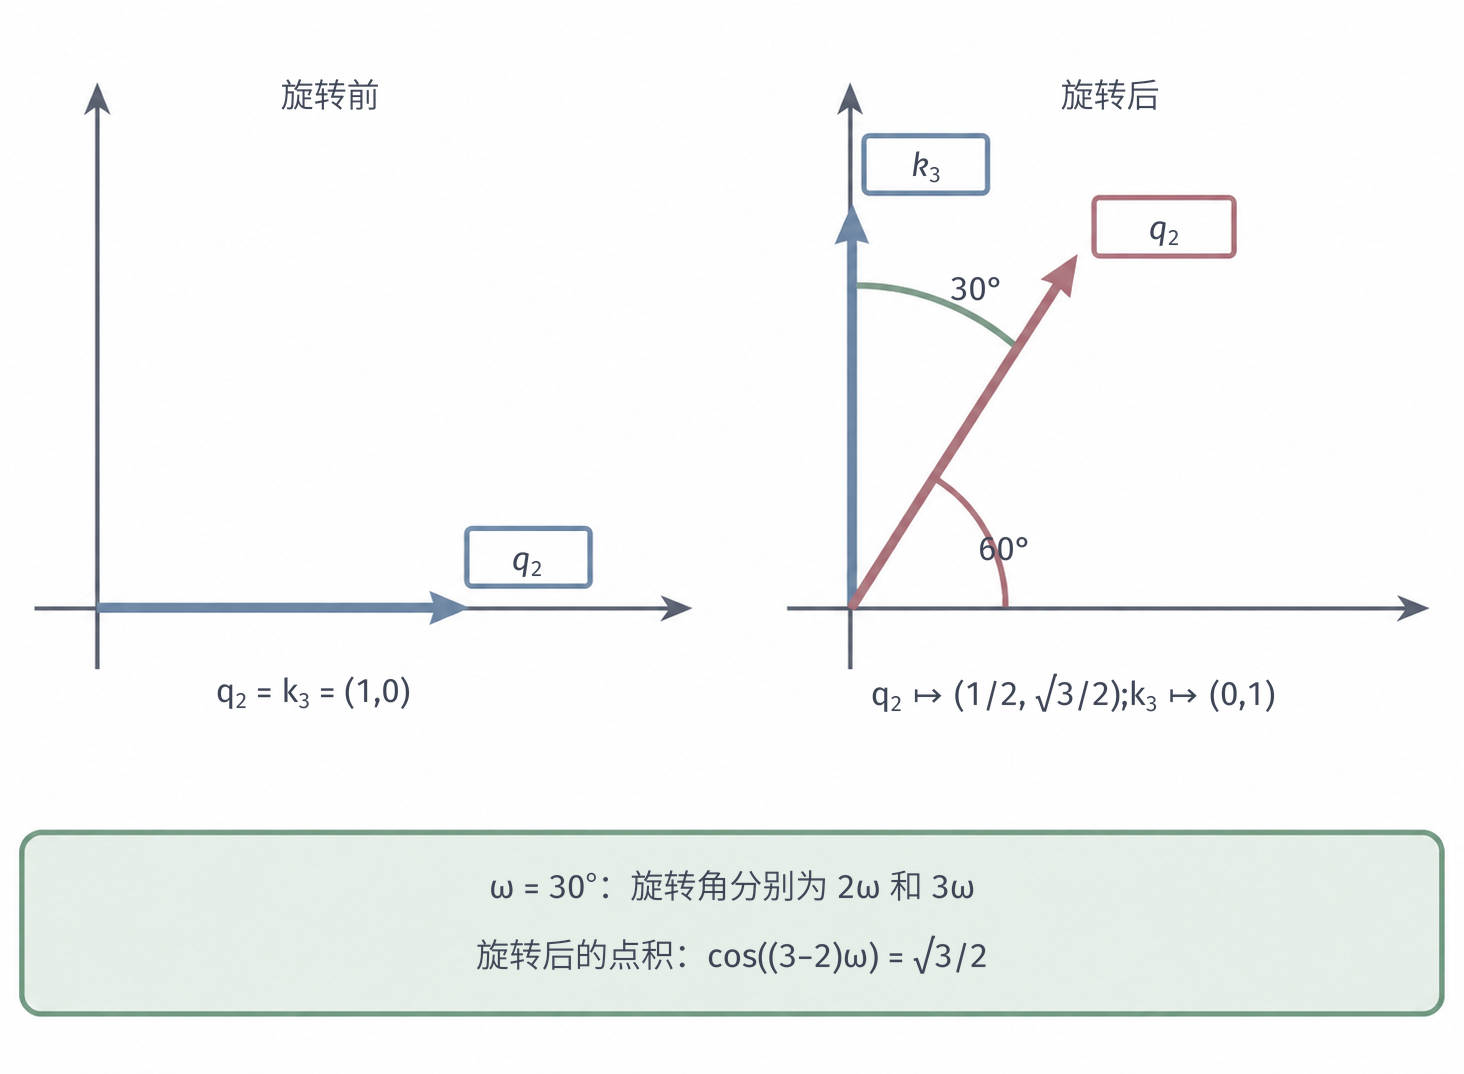
\includegraphics[width=112.000mm]{figures/03-models/02-neural-network-models/generated/transformer-rope/figure.png}
  \caption{RoPE在一个二维坐标对中的作用。左图两个内容向量重合；右图“追”的查询和“狗”的键按各自位置旋转，夹角为$(3-2)\omega=30^\circ$，点积因此依赖相对位置。示例频率为$\pi/6$，用于演示几何关系；实际模型对多个坐标对采用不同频率，并保留各自的内容向量。}
  \label{fig:transformer-rope}
\end{figure}
\FloatBarrier

绝对与相对描述的是位置关系，旋转描述的是注入机制，一个按绝对编号执行的旋转，可以在点积中形成相对距离关系。可学习绝对表有显式长度参数，固定正弦和RoPE无需位置表，距离偏置由距离覆盖或斜率决定参数量；位置计算的资源与覆盖范围可以据此比较，训练长度外的误差则还需要任务和数据条件。图像还需要保留二维位置，连续时间数据需要处理实际时间间隔，单一序列编号未必足够。



\subsection{注意力机制的扩展}
\label{sec:transformer-attention-extensions}

完整序列计算同时有$n$个查询；逐步解码通常只增加一个查询，但仍要读取历史键和值。\term{键值缓存}（key--value cache, KV cache）保存每层已有位置的键和值，生成时只计算新位置的投影并追加。固定参数、位置编号和因果掩码时，旧位置表示不依赖未来输入，所以其键值可以复用；如果前缀内容或可见规则改变，原缓存未必继续有效。

对$L$层、$h$头、每头$d_k=d_v$、当前长度$n$的单序列，标准缓存有$2Lnhd_k$个元素，字节量还要乘以每元素的存储字节数和批量大小。旧位置的投影与网络块结果可直接复用，新查询则继续读取$n$个键和值，其位置对算术量为$O(nhd_k)$。将长度从1生成到$n$时，稠密注意力累计仍有平方量级的位置对读取。预填充（prefill）是一次处理已知前缀并建立缓存，逐步解码（decoding）则复用缓存产生后续内容；两者的并行规模和存储瓶颈不同。

\subsubsection{模型效果：信息范围与特征选择}

\paragraph{支持不同信息来源与可见范围}

交叉注意力改变键值来源，因果注意力改变允许的连接，两者可以同时出现于同一目标块。\term{前缀注意力}（prefix attention）让给定条件前缀内部互相读取，而目标位置读取前缀和此前目标；前缀表示只由条件前缀形成；若加入目标信息，原来的前缀表示便会改变，需要重新编码。图~\ref{fig:transformer-masks}固定“猫／追／狗／EOS”四个位置，对比三种掩码。前缀方案把“猫追”设为已知条件，两位置内部可以互读；生成“狗”时可以读取这段条件，而“狗”的信息不能反向进入已缓存的条件表示。掩码将条件输入与生成前缀的可见范围直接写入每层计算。

\begin{figure*}[htbp]
  \centering
  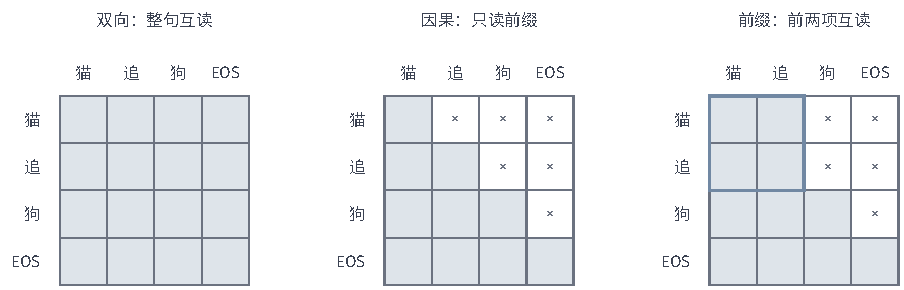
\includegraphics[width=153.003mm]{figures/03-models/02-neural-network-models/tikz/transformer-masks/figure.pdf}
  \caption{四个位置的读取范围。行表示查询位置$i$，列表示键位置$j$，着色格允许读取，带叉白格禁止读取。左为全部有效输入间的双向读取，中为$j\leq i$的因果读取，右为前两个位置构成条件前缀的读取：前缀内部双向，目标读取全部前缀与截至当前位置的目标输入。目标输入已移位，因此读取当前输入不等于读取当前待预测标签。}
  \label{fig:transformer-masks}
\end{figure*}
\FloatBarrier

\paragraph{优化动态信息选择：门控注意力}

Softmax每行必须把总权重1分配给可见值，即使这些值都不适合当前更新。\term{门控注意力}（gated attention）增加一个输入相关的控制量，调节特征或聚合结果的通过程度。例如，对第$a$头在位置$i$的结果，可以令
\begin{equation}
  \bm g_{i,a}=\sigma(\bm W_{\mathrm g,a}^{\top}\bm h_i+\bm b_{\mathrm g,a}),\qquad
  \widetilde{\bm z}_{i,a}=\bm g_{i,a}\odot\bm z_{i,a}\text{，}
  \label{eq:transformer-gated-attention}
\end{equation}
其中$\bm W_{\mathrm g,a}\in\mathbb R^{d\times d_v}$，Sigmoid门与头输出同宽。每头一个标量门则把整头共同缩放。注意力权重选择“从哪些位置读取”，输出门决定“这次读取的哪些特征应通过”，两者作用对象不同。

门也可置于值投影之后或最终输出投影之后，这些位置通常不等价。值门改变不同来源的内容，查询相关的输出门改变接收端结果。Qiu等比较了门的位置和粒度，并在所测试的大语言模型配置中观察到聚合后Sigmoid门对训练与表示行为的改善；观察到的改进对应论文中的训练配置，其作用范围由模型、目标及数据确定。逐坐标门增加非线性和参数，也要考虑饱和造成的梯度减弱\scite{qiu2025gated}

图~\ref{fig:transformer-gated-attention}接着使用“追”的聚合结果$(0.5,1.25)^{\top}$。若当前表示生成的门为$(0.2,0.8)^{\top}$，逐坐标相乘得到$(0.1,1.0)^{\top}$，分别保留第一维的20\%与第二维的80\%。位置权重在此前已经完成归一化，门按坐标调整混合后的特征，来源位置的权重仍由前面的Softmax给出。标准点积和键值存储都已在门控前完成，其成本继续保留。

\begin{figure*}[htbp]
  \centering
  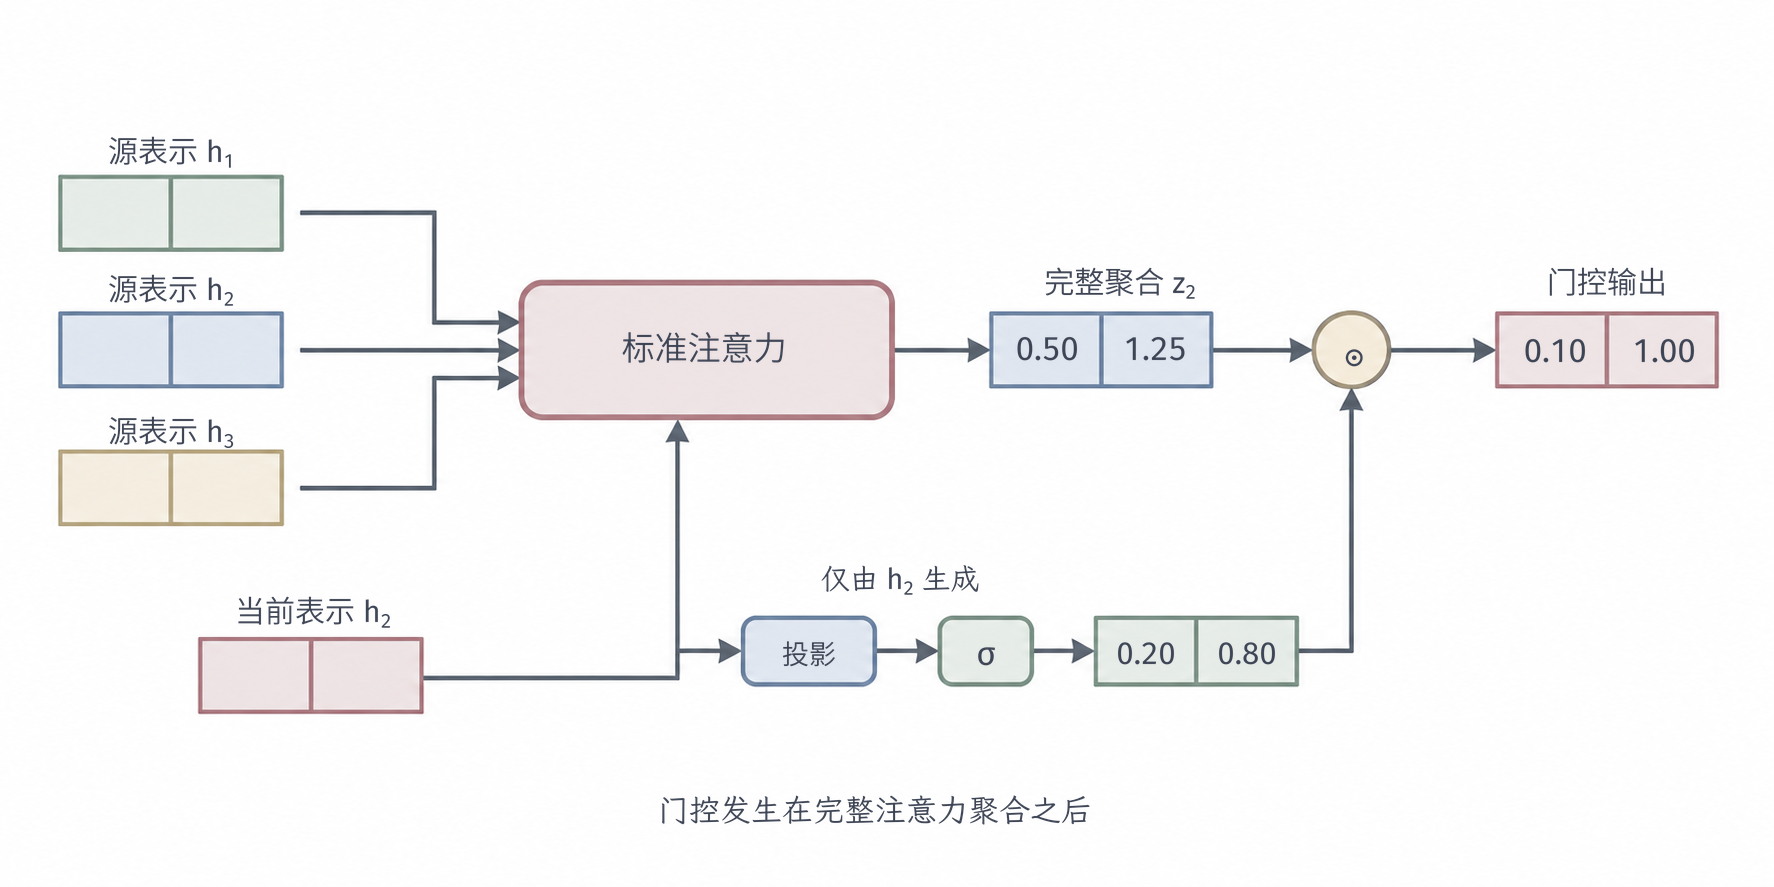
\includegraphics[width=150.199mm]{figures/03-models/02-neural-network-models/generated/transformer-gated-attention/figure.png}
  \caption{以“追”为查询的聚合后门控。左支路从整段序列读取内容，右支路仅由当前词元表示产生Sigmoid门。教学数值中，聚合结果$(0.5,1.25)$与门$(0.2,0.8)$逐坐标相乘，得到$(0.1,1.0)$。门控制的是输出特征，而不是三个来源位置的概率；图中固定一个头并省略头索引、多头拼接和输出投影，数值并非训练测量。}
  \label{fig:transformer-gated-attention}
\end{figure*}
\FloatBarrier

\subsubsection{训练效率：位置交互与中间存储}

整段训练需要为位置对评分，还要为反向保存或重算中间量。连接数影响前一成本，聚合公式与执行方式影响后者及其访存；下面分别说明这些改动在训练和推理中的适用范围。

\paragraph{降低位置连接的计算量：稀疏注意力}

\term{稀疏注意力}（sparse attention）只计算保留的连接。例如每个位置读取$w$个窗口位置，再加少量全局位置，若各头保留连接总数为$e_{\mathrm{att}}$，评分和聚合需要$O(e_{\mathrm{att}}(d_k+d_v))$算术操作，权重存储为$O(e_{\mathrm{att}})$。窗口大小和全局连接数固定时，连接数随$n$线性增长；窗口若随$n$增长，复杂度也相应保留窗口长度因子。Sparse Transformer采用特定稀疏分解，使连接数达到$O(n\sqrt n)$量级，其稀疏连接仍多于固定窗口的线性规模$O(n)$\scite{child2019sparse}

删除连接也改变传播范围。只有窗口连接时，一层无法读取窗口之外的信息，跨层传播可扩大范围，却增加依赖路径长度；全局位置使远处信息有较短通路，但也可能形成汇总瓶颈。保留哪些连接决定哪些证据能够到达目标位置，相同比例的稀疏模式也可能形成不同通路。

\paragraph{降低聚合计算量：线性注意力}

\term{线性注意力}（linear attention）把位置对核改写为有限维特征内积，以改变聚合次序。设$\phi(\bm q),\phi(\bm k)\in\mathbb R^r$，内积非负且分母为正，则可定义
\begin{equation}
  \begin{aligned}
    \bm T&=\sum_{j=1}^n\phi(\bm k_j)\bm v_j^{\top},\qquad
    \bm b=\sum_{j=1}^n\phi(\bm k_j),\\
    \bm z_i^{\top}&=\frac{\phi(\bm q_i)^{\top}\bm T}
                           {\phi(\bm q_i)^{\top}\bm b}\text{。}
  \end{aligned}
  \label{eq:transformer-linear-attention}
\end{equation}
$\bm T\in\mathbb R^{r\times d_v}$和$\bm b\in\mathbb R^r$先汇总键值，再被所有查询读取。除特征映射和输入输出投影外，单头算术量为$O(nrd_v+nr)$，中间汇总存储为$O(rd_v+r)$；固定$r,d_v$时，这里的成本对$n$线性；特征映射和归一化仍使输出可以是输入的非线性函数。保存所有位置的激活和训练梯度还需额外存储。

因果读取把上述和限制到$j\leq i$，得到$\bm T^{(i)}=\bm T^{(i-1)}+\phi(\bm k_i)\bm v_i^{\top}$、$\bm b^{(i)}=\bm b^{(i-1)}+\phi(\bm k_i)$。它可用固定大小的状态逐步生成，也可在整段输入上做前缀扫描。Katharopoulos等给出了这类计算与循环形式的联系；有限维特征核使聚合次序可以交换；标准Softmax一般需要相应近似，或者由另一种核替代\scite{katharopoulos2020linear}

\paragraph{压缩位置交互表示：低秩注意力}

\term{低秩注意力}（low-rank attention）用较小的交互表示代替全部位置。例如Linformer在位置维上用$\bm E_{\mathrm k},\bm E_{\mathrm v}\in\mathbb R^{r\times n}$分别压缩键和值，形成$\overline{\bm K},\overline{\bm V}$，再计算$n\times r$的注意力。固定各头配置时，位置压缩、评分和聚合的量级可降为$O(nr(d_k+d_v))$。它依赖低秩近似是否适合输入，并改变了可读取的表示\scite{wang2020linformer}

压缩槽若含未来键值，查询读到这个槽时也会间接读到未来；槽之间的三角掩码无法拆开已混合内容。因果方案需要在压缩阶段就限制信息范围。压缩矩阵还可能绑定最大长度，$r$若为保持精度随$n$增长，实际复杂度也随之改变。删连接限制位置通路，换核限制匹配形式，压缩槽限制被读取表示。相同任务和有效长度使这些取舍能够对应到共同误差与成本。

图~\ref{fig:transformer-efficient-attention}把三条路线放回同一句“猫在院里追狗”，按字分成6个位置。左侧局部连接只保留当前位置及其左右邻居，把36个位置对减到16个；“追”这一行可以读取“里、追、狗”，却不能在本层直接读取“猫”。中间线性路线为键特征和值设置可手算的二维数值。六项外积累加为$\bm T=\bigl[\begin{smallmatrix}6&3\\3&6\end{smallmatrix}\bigr]$，键特征相加为$\bm b=(4,4)^{\top}$；查询特征$(1,1)^{\top}$因而得到$(9/8,9/8)^{\top}$。这里各位置共同贡献一个固定大小的状态，查询再从状态读取。

右图则直接压缩位置：教学投影把前三个位置、后三个位置分别取平均，形成两个键值槽。所有6个查询仍各有一行，但每行只向两个槽评分。图中为便于核对令$\bm E_{\mathrm k}=\bm E_{\mathrm v}=\bm E$；Linformer的投影可以学习，也不必采用局部平均。这三幅图分别改变连接、核与可读取的表示，矩阵缩小分别来自删连接、改变核或合并位置，三个输出由各自的新计算定义。

\begin{figure*}[p]
  \centering
  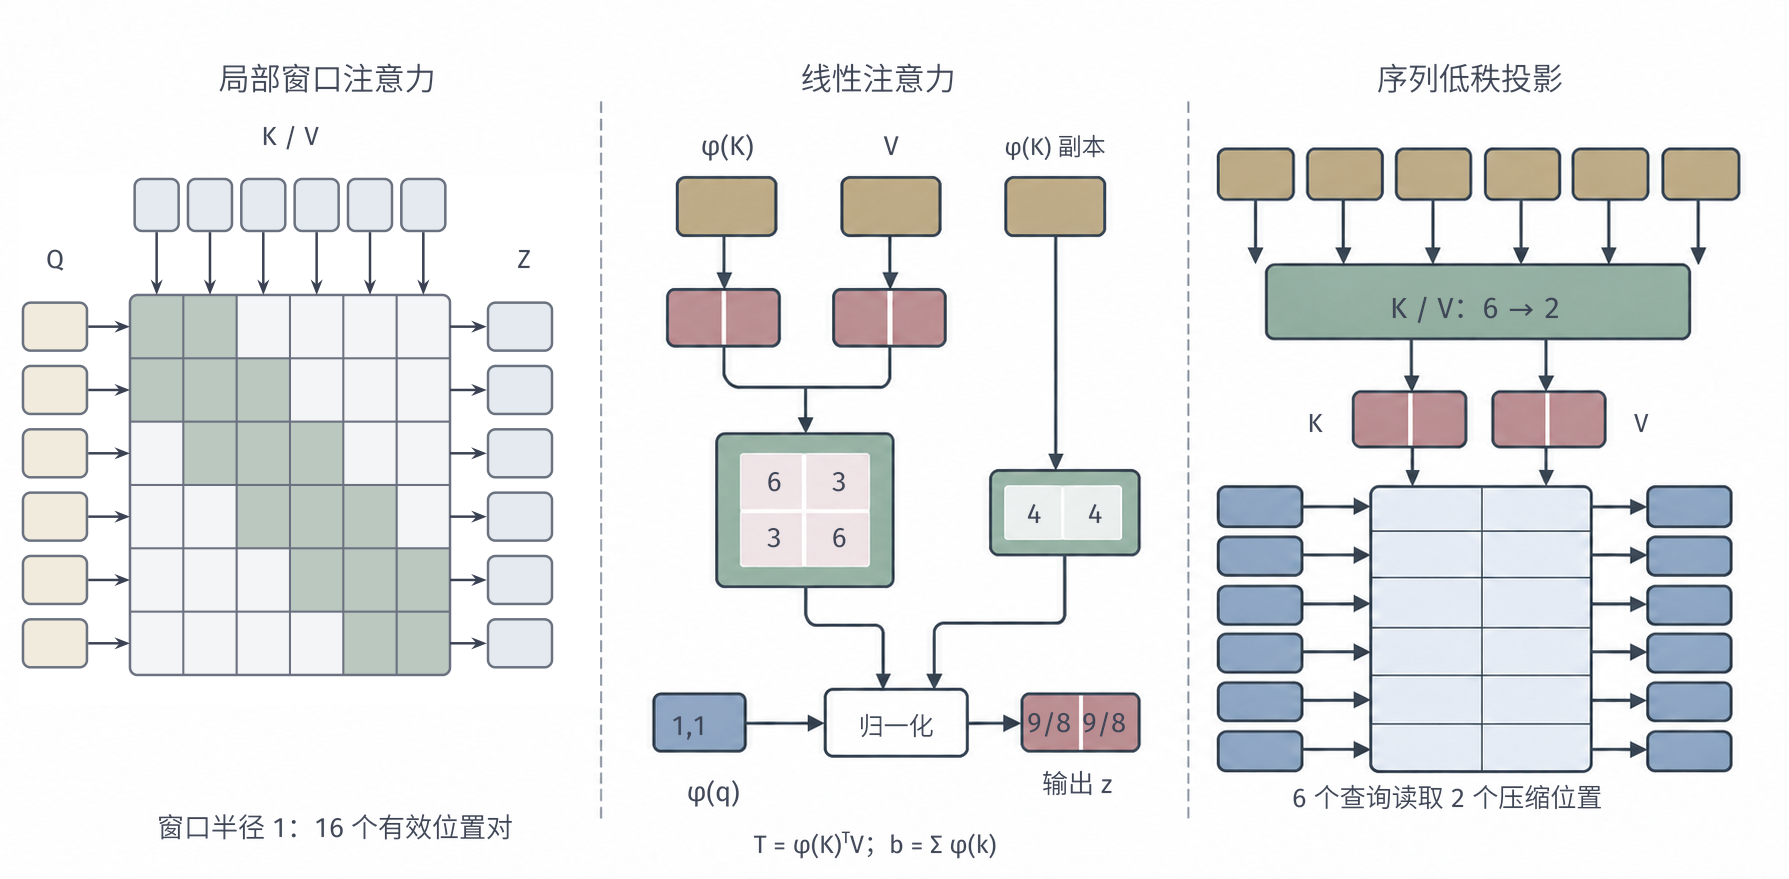
\includegraphics[width=151.469mm]{figures/03-models/02-neural-network-models/generated/transformer-efficient-attention/figure.png}
  \caption{三条效率路线的具体读法，六个位置可按正文的“猫／在／院／里／追／狗”教学序列理解。左图中查询$\bm Q$对应各行，键值$\bm K/\bm V$对应各列，输出$\bm Z$逐行引出；着色格保留相邻位置的连接，白格表示删除的连接。中图给定教学键特征和值后，先累加外积和特征，再对查询归一化，数值由式\eqref{eq:transformer-linear-attention}复核。右图的示例投影把6个位置压成2个槽，右侧每行表示一个查询对两槽评分，颜色只表示存在连接。所有数值及压缩权重均为教学设定；三种方法并非对同一Softmax结果的等价改写。}
  \label{fig:transformer-efficient-attention}
\end{figure*}
\FloatBarrier

\paragraph{优化中间存储与访存：FlashAttention}

前面三条路线改变了读取规则或公式。\term{FlashAttention}保留标准稠密注意力的数学结果，通过分块计算和在线归一化，避免把完整得分、概率矩阵写入大容量显存。它在容量较小的片上存储中反复处理查询和键值块，减少完整中间矩阵的显存读写；反向传播按需要重算部分块，保存的统计量支持恢复这些局部计算\scite{dao2022flashattention}

理解在线Softmax可以只看一个查询。已处理的键集合上，维护最大得分$m$、归一化分母$s=\sum_j\exp(S_j-m)$和未归一化输出$\bm u=\sum_j\exp(S_j-m)\bm v_j$。新键块集合为$B$，块内最大值为$m_B$，更新为
\begin{equation}
  \begin{aligned}
    m'&=\max(m,m_B),\qquad c=\exp(m-m'),\\
    s'&=cs+\sum_{j\in B}\exp(S_j-m'),\\
    \bm u'&=c\bm u+\sum_{j\in B}\exp(S_j-m')\bm v_j\text{。}
  \end{aligned}
  \label{eq:transformer-online-softmax}
\end{equation}
旧统计乘以$c$，是在新最大值下重新表达同一批指数。遍历全部有效块后，输出为$\bm u/s$。初始为空时直接用第一个非空有效块建立统计，避免在全被掩码的块上做$-\infty-(-\infty)$。

沿用示例~\ref{ex:transformer-attention-numerical}，先处理得分$0,\log2$，得到$m=\log2$、$s=3/2$、$\bm u=(1/2,2)^{\top}$；再加入得分0和值$(1,1)^{\top}$，得到$s'=2$、$\bm u'=(1,5/2)^{\top}$，仍输出$(1/2,5/4)^{\top}$。分块没有把不同块分别归一化后简单求和，而是维护全局共同分母。

在固定头数和宽度下，FlashAttention把需要保存的注意力中间量从平方规模降到线性规模，实际训练还需保存其他模块激活。稠密位置对仍然存在，算术量仍为$O(n^2d)$；浮点运算顺序改变，结果可能有舍入差异。这里的“精确”指保留原稠密注意力公式，浮点舍入按实际执行顺序发生。速度收益依赖块大小、硬件和输入形状，其加速针对数据搬运与存储，位置对算术阶数保持原样。

图~\ref{fig:transformer-flashattention}对比“保存整个中间矩阵”与“算完一块就合并”。左侧常规路径显式形成完整得分与概率矩阵，右侧分块路径维护同一组$m,s,\bm u$，跨块更新使最终分母覆盖所有键；旧统计按新最大值重新缩放后，新旧键共同进入同一分母。对其他查询块重复这一过程，就能得到完整输出，而无需让完整得分、概率矩阵在大容量显存中落地。

\begin{figure*}[htbp]
  \centering
  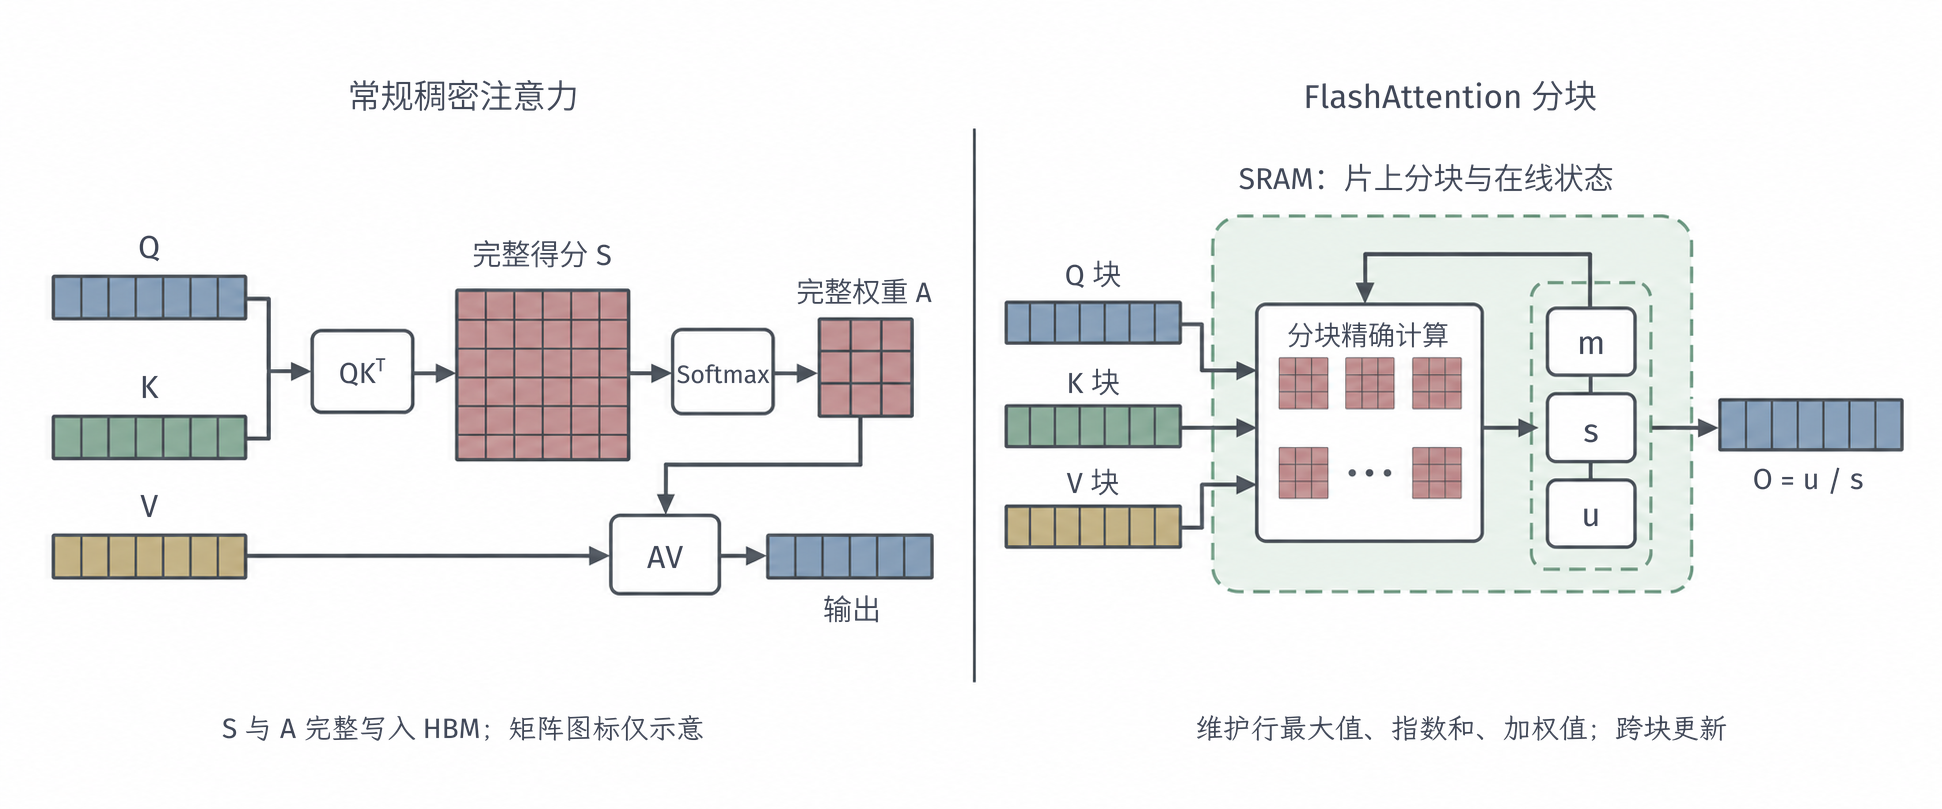
\includegraphics[width=164.423mm]{figures/03-models/02-neural-network-models/generated/transformer-flashattention/figure.png}
  \caption{FlashAttention保留稠密注意力结果，改变中间结果的存储与合并方式。左图的常规实现把完整$\bm S,\bm A$写回容量较大的HBM；右图按块在HBM与容量较小的片上SRAM间搬运，只在片上保存当前块和在线统计$m,s,\bm u$。在线合并的分母覆盖全部键，输出与同一稠密注意力计算一致。图为存储与计算路径示意，教学数值在正文展开，反向重算细节省略。}
  \label{fig:transformer-flashattention}
\end{figure*}


\FloatBarrier

\subsubsection{推理效率：历史缓存与请求分配}

增量生成需要反复读取历史键值，还要为不同长度请求分配存储。以下方法分别改变缓存内容与存储组织。

\paragraph{减少KV缓存容量与读取带宽：MQA与GQA}

解码时，标准MHA为每头保存一套键和值。\term{多查询注意力}（multi-query attention, MQA）保留多个查询头，让它们共享一组键值；\term{分组查询注意力}（grouped-query attention, GQA）将$h$个查询头分组，共享$g$组键值，其中$1\leq g\leq h$。设映射$\rho(a)$把查询头$a$分到键值组，则该头读取$\bm K_{\rho(a)},\bm V_{\rho(a)}$，仍有自己的一行Softmax和输出。

当$d_k=d_v$时，缓存元素数由$2Lnhd_k$变为$2Lngd_k$；MQA对应$g=1$，MHA对应$g=h$。例如$L=24$、$n=4096$、$h=16$、$d_k=64$、每元素2字节的单序列MHA缓存约为384 MiB，$g=4$的GQA约为96 MiB，MQA约为24 MiB。这组教学容量由键值元素数计算；权重、其他激活及分配管理另占存储。

图~\ref{fig:transformer-kv-sharing}固定3个历史位置“猫、追、狗”和4个新查询头，逐项数缓存中的键值对。MHA为每头保留3对，共12对；两组GQA保留6对；MQA只保留3对。MHA中同一历史位置对应4个缓存小格，表示该位置经过4组不同投影后产生的4对键值，四组投影分别产生自己的数值。共享后，不同查询仍分别与所读键匹配，所以可能得到不同的概率和输出。

\begin{figure*}[p]
  \centering
  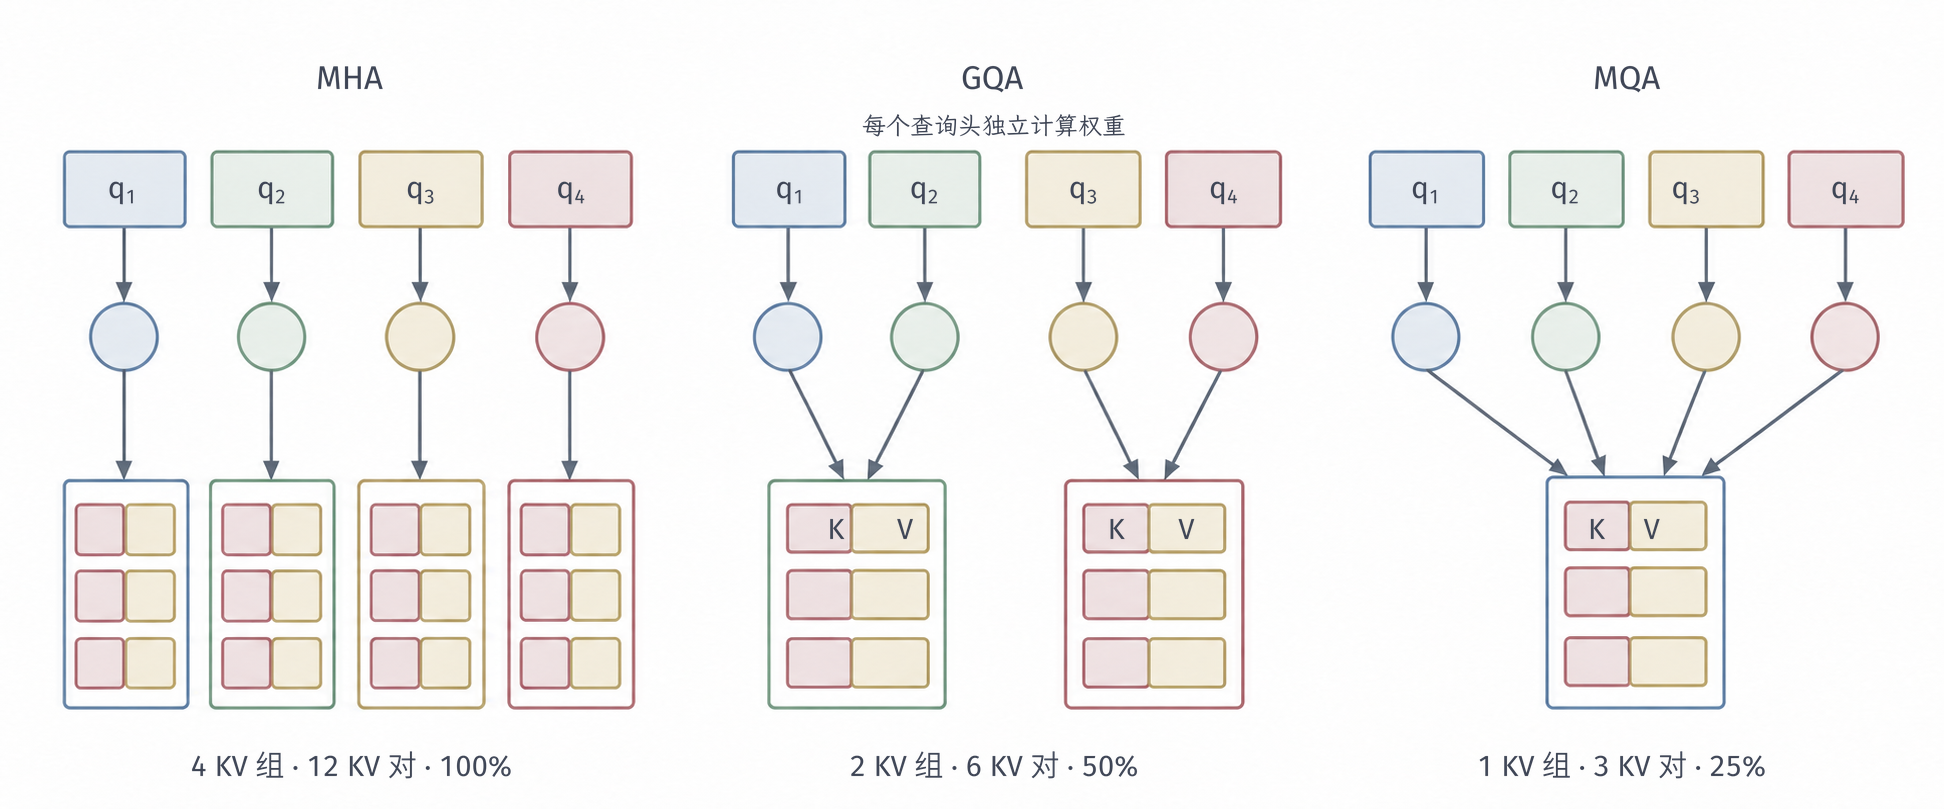
\includegraphics[width=164.592mm]{figures/03-models/02-neural-network-models/generated/transformer-kv-sharing/figure.png}
  \caption{相同历史序列在MHA、GQA和MQA中的缓存布局。每个缓存小格代表一个历史位置在一组投影下的一对键和值；大框是一整组历史缓存，查询头的箭头指向所读取的缓存。4个查询头分别使用4组、2组或1组键值时，缓存为12、6或3对，下方标出的缓存容量相对于MHA依次为$100\%$、$50\%$和$25\%$。共享发生在键值表示及其存储上，各查询头仍独立计算注意力权重。图只计一层的一条序列，不含当前新位置追加的缓存。}
  \label{fig:transformer-kv-sharing}
\end{figure*}
\FloatBarrier

Shazeer提出MQA以减少增量解码的键值访存，Ainslie等用GQA提供共享程度与质量之间的中间选择。共享减少了键值投影和缓存自由度，但查询头仍需分别匹配；查询仍逐头评分，评分算术量与缓存容量的$g/h$比例因此按不同操作统计。缓存读取若能在实现中复用，带宽需求才会相应改善，质量和速度都需要在给定模型与硬件上评价\scite{shazeer2019mqa} GQA还可由已有多头模型进行参数转换并继续训练，键值参数合并会改变表示，后续训练用于适应新的共享结构\scite{ainslie2023gqa}

\paragraph{提高KV缓存内存利用率：PagedAttention}

缓存容量之外，还存在分配问题：不同请求的长度持续增长，为每个请求预留连续最大空间会留下空闲区域，共同前缀还可能被多次保存。\term{分页注意力}（PagedAttention）把缓存划分为固定容量块，用块表把序列的逻辑位置映射到实际存储位置；序列增长时追加块，而不要求整段缓存连续。共同前缀可以引用同一批块，分叉后按需要复制，避免直接修改仍被其他请求读取的数据\scite{kwon2023pagedattention}

若每块容纳$b$个位置，长度$n$需要$\lceil n/b\rceil$块，最后一块的内部空余少于$b$个位置，另有块表和管理开销。原来连续存储中的外部碎片和重复前缀可由此减少，实际键值按所保存的位置继续占据空间，节省的是预留空闲、碎片和重复前缀。PagedAttention改变缓存寻址和共享，MQA/GQA改变键值组数，FlashAttention改变注意力中间结果的执行方式；三者处理不同问题，可在兼容实现中组合。块调度、并发服务和硬件算子的细节由系统卷展开。

图~\ref{fig:transformer-pagedattention}用两个请求演示块表的作用。为便于说明，把“请／解释／注意力／机制”和“请／解释／位置／编码”各视为4个词元，每块放2个位置。本图的词元位置与逻辑块均从0编号。A按物理块$3\rightarrow1$读取，B按$3\rightarrow4$读取，两者共享前缀块3，物理块2仍可供其他请求使用。读取A中位置$i=1$的“解释”时，逻辑块为$\lfloor1/2\rfloor=0$，块内偏移为1；查A块表索引0得到物理块3，再从其中的偏移1取出键和值。词元位置给出逻辑顺序，块表给出物理地址；物理块移动时保持块表对应，位置编码继续使用原逻辑编号。

\begin{figure*}[htbp]
  \centering
  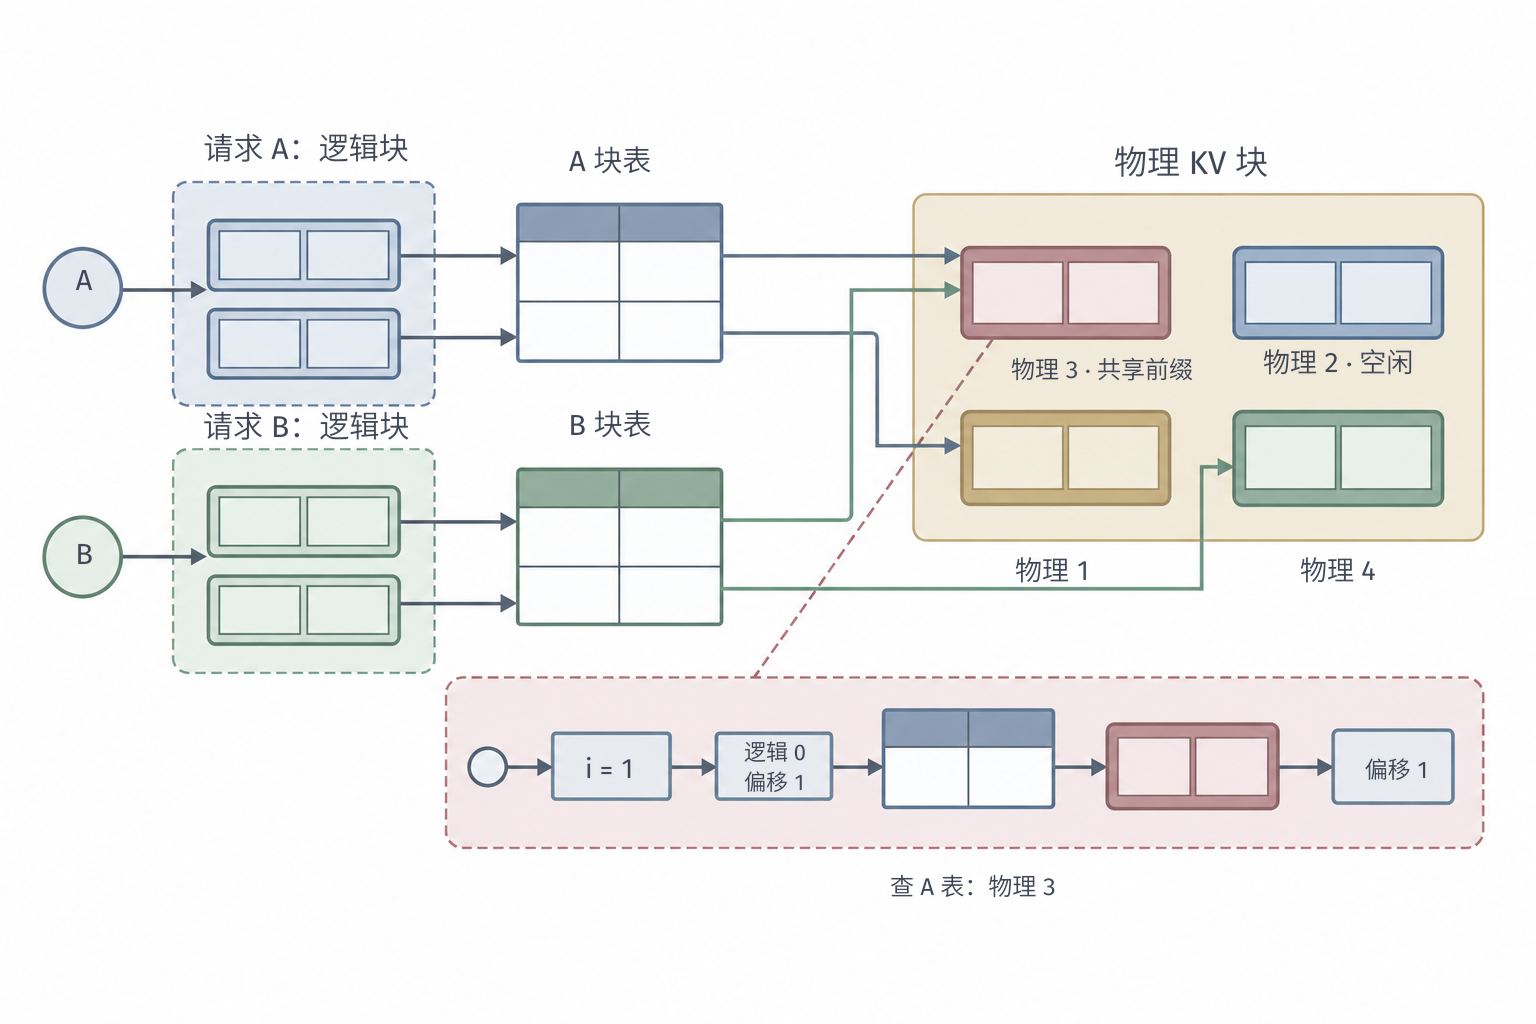
\includegraphics[width=130.048mm]{figures/03-models/02-neural-network-models/generated/transformer-pagedattention/figure.png}
  \caption{分页键值缓存的具体寻址。上方两条请求按逻辑顺序分块，并用块表保存物理块编号；右侧为实际缓存布局。共享的物理块3只保存一份，A、B的后续各占一块，无需保持物理连续。底部展开一次“位置$\rightarrow$逻辑块$\rightarrow$物理块及偏移”的查找。词元位置、逻辑块和表索引从0开始；物理块编号用1至4标识。缓存小格表示对应的KV内容，正文中的词元例子用于解释寻址，并非把原始文本当作键值向量。}
  \label{fig:transformer-pagedattention}
\end{figure*}
\FloatBarrier

\paragraph{不同扩展方向的比较}

表~\ref{tab:transformer-attention-extensions}把模型变化与实现变化分开。长序列算术量由实际位置连接与聚合决定，FlashAttention改善中间访存，分页改善键值分配。训练概率矩阵与解码历史缓存也有不同生命期，缩小其中一种只节省相应存储。门控、GQA、FlashAttention和分页可以在兼容实现中组合，因为它们分别作用于特征选择、键值组织、块内计算和缓存寻址。

\begin{table*}[htbp]
  \centering
  \small
  \begin{tabular}{@{}p{30mm}p{37mm}p{39mm}p{49mm}@{}}
    \toprule
    方法 & 主要改善对象 & 改变标准稠密读取？ & 代价或限制 \\
    \midrule
    前缀等掩码 & 可用信息与任务约束 & 改变允许连接 & 需防止目标或跨段泄漏 \\
    门控注意力 & 输入相关的特征选择 & 增加乘性调制 & 增加参数；不自动减少连接 \\
    稀疏注意力 & 位置对算术量 & 删除部分连接 & 范围受限；依赖连接模式 \\
    线性注意力 & 聚合算术量及历史状态 & 改变核或近似Softmax & 依赖特征维$r$与核表达能力 \\
    低秩注意力 & 交互维度与算术量 & 压缩键值位置 & 近似误差；因果性需另设计 \\
    FlashAttention & 中间存储与显存访存 & 保持公式，舍入可能不同 & 稠密算术仍为平方量级 \\
    MQA/GQA & KV容量与解码带宽 & 跨头共享键值参数 & 改变自由度；评分仍按查询头 \\
    PagedAttention & 缓存分配与前缀共享 & 保持逻辑读取规则 & 块表管理；真实键值仍占空间 \\
    \bottomrule
  \end{tabular}
  \caption{注意力扩展的主要目标与取舍。比较以相同有效输入、隐藏宽度与预测条件为前提；具体算术和存储量见各方法正文。降低算术量、减少访存、缩小KV缓存和减少内存碎片是不同指标，实际速度还取决于实现与硬件。}
  \label{tab:transformer-attention-extensions}
\end{table*}
\FloatBarrier

\subsection{前馈层的扩展}
\label{sec:transformer-ffn-extensions}

同一位置的特征可以通过乘法分支调制，也可以交给少量被选中的前馈网络。门控改变特征变换形式，混合专家改变本次执行的网络分支；二者可以组合，跨位置读取仍由注意力等模块承担。

\subsubsection{门控前馈层：调制特征}

普通FFN先扩张特征，再用统一激活筛选。若希望同一输入同时决定候选特征和通过程度，可以设置两条投影分支。\term{门控线性单元}（gated linear unit, GLU）用Sigmoid分支逐坐标调制另一分支；应用于Transformer前馈层的一般形式为
\begin{equation}
  \begin{aligned}
    \bm B&=\bm H\bm W_b+\bm1\bm b_b^{\top},\qquad
    \bm D=\bm H\bm W_g+\bm1\bm b_g^{\top},\\
    \operatorname{GFFN}(\bm H)&=(\bm B\odot\psi(\bm D))\bm W_o
                          +\bm1\bm b_o^{\top}\text{。}
  \end{aligned}
  \label{eq:transformer-gated-ffn}
\end{equation}
两条输入投影均从$d$到$d_g$，输出投影从$d_g$恢复$d$。GLU取$\psi=\sigma$，\term{GEGLU}取GELU，\term{SwiGLU}取SiLU，后两者分别由平滑激活产生乘性调制量。GELU或SiLU可以输出负值且不限定在$[0,1]$，这里的“门控”据乘法作用命名；LSTM的Sigmoid门另外受0至1的比例范围约束\scite{shazeer2020glu}

忽略偏置时，普通FFN约有$2dd_f$个参数，门控FFN约有$3dd_g$个参数。若保持这一参数预算，可取$d_g\approx2d_f/3$；比较同样中间宽度会同时改变参数和计算量。两投影分支提供新的特征组合，同时带来乘法尺度与参数配置的选择。泛化表现需结合相同预算下的任务与训练比较。

图~\ref{fig:transformer-gated-ffn}把“追”这一行的两条分支展开：候选特征$(2,-4)$与调制量$(0.5,2)$相乘，得到$(1,-8)$，再经输出投影恢复$d$维。第二维被放大，说明GEGLU、SwiGLU中的调制量不只是保留比例。这里用二维数值演示乘法，实际中间宽度由$d_g$决定；各位置仍独立处理，没有新增跨位置读取。

\begin{figure}[htbp]
  \centering
  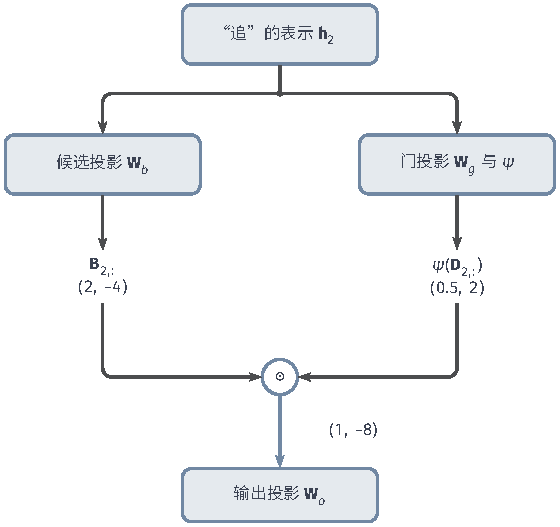
\includegraphics[width=94.791mm]{figures/03-models/02-neural-network-models/tikz/transformer-gated-ffn/figure.pdf}
  \caption{门控前馈层对“追”的一次逐位置计算。候选特征$(2,-4)$与激活后的调制量$(0.5,2)$相乘为$(1,-8)$，再经输出投影恢复隐藏宽度。数值是教学假设；大于1的调制量适用于GEGLU或SwiGLU的解释，GLU的Sigmoid门则限制在0与1之间。猫、追、狗使用同一套参数分别计算，不发生跨位置读取。}
  \label{fig:transformer-gated-ffn}
\end{figure}
\FloatBarrier

\subsubsection{混合专家：前馈层的条件计算}
\label{sec:transformer-moe-extensions}

逐位置计算还可以按输入选择不同前馈网络。\term{混合专家}（mixture of experts, MoE）设置多个专家和一个路由器，让不同位置使用不同专家组合。\term{专家}（expert）是可训练的特征变换网络，\term{路由器}（router）根据位置表示分配专家权重。设共有$e$个专家，单位置为$\bm h$，路由概率为$\bm p=\operatorname{softmax}(\bm W_{\mathrm r}^{\top}\bm h)$，$\bm W_{\mathrm r}\in\mathbb R^{d\times e}$。若只保留分数最大的$k$个专家集合$T_k(\bm h)$，可以计算
\begin{equation}
  \operatorname{MoE}(\bm h)
    =\sum_{a\in T_k(\bm h)}\widetilde p_a\,F_a(\bm h)\text{，}
  \label{eq:transformer-moe}
\end{equation}
其中$\widetilde p_a$可取选中概率重新归一化后的权重，也可按具体方法保留原概率；训练性质依赖这一约定。总专家参数随$e$增长，一次位置计算主要激活$k$个专家，加上路由器及共享模块的开销，模型存储计入全部专家，本次执行量按被选专家及公共部分分别统计\scite{shazeer2017}

路由可能把大量位置分给少数专家，造成容量不足或计算负载不均。容量限制决定多余位置如何处理，负载均衡辅助目标约束专家使用分布；它们会改变训练目标或输出过程。Top-$k$选择是离散的，常规反向传播只能在当前选择内对连续权重和专家求导，跨越选择边界的行为需要单独设计。若$k=1$并将唯一概率重新归一化为1，仅从这条乘权路径无法训练路由器，尤其需要保留可学习权重或其他训练信号。专家接到哪些输入、形成何种变换，由路由和监督共同学习。设备间派发与汇总还产生通信及调度成本，需在实际执行中另计。

图~\ref{fig:transformer-moe}把路由决策与专家计算分开。对“追”的同一个隐藏表示，假设路由概率为$(0.1,0.6,0.1,0.2)$。Top-2选择专家2和4，再除以所选概率之和$0.8$，得到权重$0.75$和$0.25$。两个专家都读取原隐藏表示$\bm h$，而不是读取路由概率；假设它们分别输出$(2,0)^{\top}$和$(0,4)^{\top}$，加权相加后才得到$(1.5,1)^{\top}$。专家1、3在本次没有执行，参数仍属于模型。这组概率与输出为手算构造，用来对应选择、执行和加权三个环节。

专家通常替换部分块中的FFN，注意力与残差仍可共享。不同位置可以选择不同专家，也可能选择相同专家；路由均衡控制位置怎样分派，输出比例继续由当前路由权重决定。

\begin{figure*}[htbp]
  \centering
  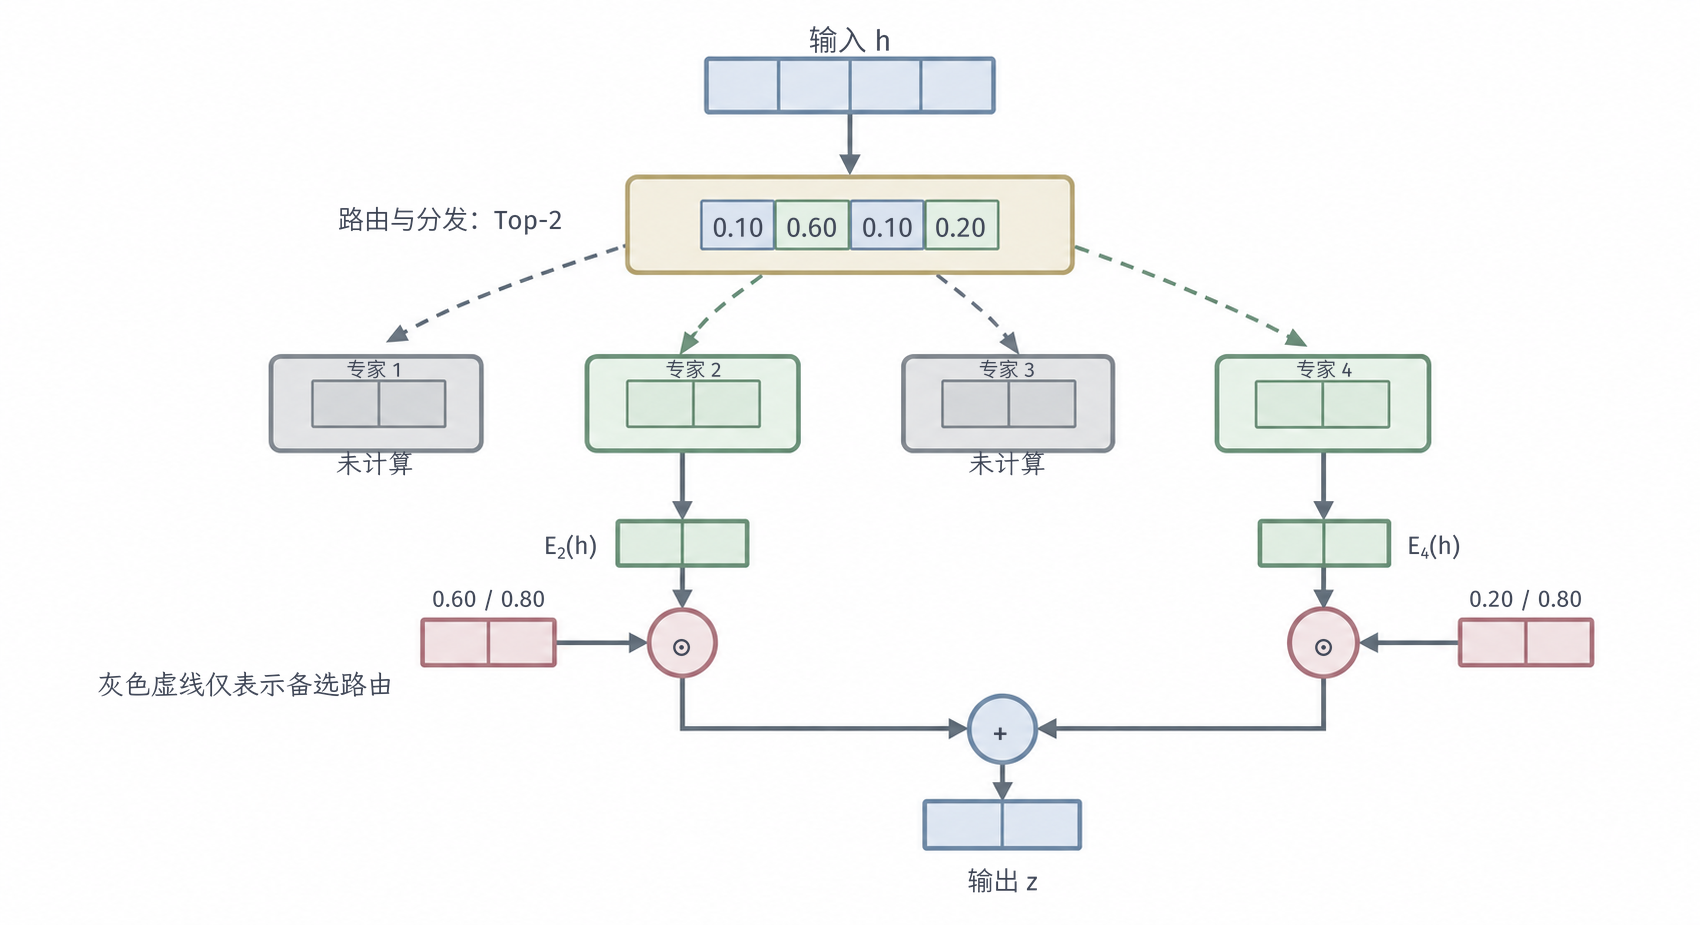
\includegraphics[width=143.933mm]{figures/03-models/02-neural-network-models/generated/transformer-moe/figure.png}
  \caption{Top-2混合专家的一次完整计算，概率与二维专家输出均为教学设定。上方路由器选出专家2、4并给出重新归一化的权重；下方实线传递隐藏表示、专家结果及乘法所需的标量权重，路由器向各候选专家的虚线表示候选选择关系。专家输入始终是同一个$\bm h$，加权发生在专家输出之后，最终$0.75(2,0)^{\top}+0.25(0,4)^{\top}=(1.5,1)^{\top}$。灰色专家1、3本次不计算；图省略容量限制、辅助训练目标及块外残差。}
  \label{fig:transformer-moe}
\end{figure*}
\FloatBarrier

\subsection{归一化的扩展}
\label{sec:transformer-normalization-extensions}

第\ref{sec:transformer-residual-normalization}节已经给出逐位置LayerNorm及其残差块形式。统计哪些坐标、是否减均值和在哪条路径归一化，决定被消去的表示变化以及信号与梯度怎样继续传递。通用归一化公式、批归一化（BatchNorm）、实例归一化（InstanceNorm）和组归一化（GroupNorm）的完整说明见第\ref{sec:training-normalization}节，统计轴对照见表~\ref{tab:training-normalization-axes}。这里集中讨论Transformer中的因果限制、RMSNorm与残差位置。

\subsubsection{统计范围与因果限制}

对批量激活$\bm X\in\mathbb R^{b\times n\times d}$，三个轴分别是样本、位置和特征。式\eqref{eq:transformer-layernorm}固定样本和位置，只沿$d$个特征统计；不同位置不交换均值与方差，训练与预测均使用当前行的统计量，不需要运行均值。在这种逐位置用法中，每份统计都只由当前样本的一行特征形成。

完整已知的图像或离线编码可以使用跨空间、跨位置统计；因果解码则要求位置$i$的统计量不能包含$j>i$的激活。只要均值或方差读取了未来，即使注意力有三角掩码也会泄漏。若BatchNorm、InstanceNorm或GroupNorm采用跨整段统计，因果解码需要把统计范围限制到当时可用的激活，并使训练与预测采用对应方案。训练用全段统计、预测用前缀统计还会引入额外不一致；填充也不能作为有效观测参与统计。

\subsubsection{不减均值的RMSNorm}

中心化不是调整尺度的唯一方式。\term{均方根归一化}（root mean square normalization, RMSNorm）不减去均值，而按坐标均方根缩放：
\begin{equation}
  \operatorname{RMSNorm}(\bm x)
    =\bm\gamma\odot\frac{\bm x}
       {\sqrt{d^{-1}\sum_{k=1}^d x_k^2+\varepsilon}}\text{。}
  \label{eq:transformer-rmsnorm}
\end{equation}
这里采用常见的无平移形式。它与逐位置LayerNorm均只读取当前行，但少了均值计算和相减。给各坐标加同一常数时，LayerNorm的中心化结果不变，RMSNorm的结果一般会变；忽略$\varepsilon$时，二者都消去正比例整体缩放，实际耗时仍由实现与形状决定\scite{zhang2019rmsnorm}

逐位置统计只读当前行，同时可能消去行内均值或整体幅度。任务需要这些量时，应保留相应信息路径或调整统计方式。只调整整行长度的尺度归一化（ScaleNorm）见第\ref{sec:training-scalenorm}节；直接重参数化权重、而非统计激活的权重归一化（WeightNorm）见第\ref{sec:training-weightnorm}节。ScaleNorm调整激活长度，WeightNorm调整参数表示，与LayerNorm消除行均值的操作分别比较。

\subsubsection{归一化位置：Pre-LN、Post-LN与组合}

归一化的位置改变残差路径。Post-LN子层$\bm y=\operatorname{LN}(\bm x+F(\bm x))$的Jacobian矩阵为$\bm J_{\mathrm{LN}}(\bm I+\bm J_F)$，直接路径也要经过LN；Pre-LN的Jacobian矩阵为$\bm I+\bm J_F\bm J_{\mathrm{LN}}$，恒等路径绕过LN。Xiong等在特定初始化与模型分析下比较了两者的梯度尺度，并解释了原始Post-LN训练中学习率预热的重要性；论文的比较对应特定初始化与模型，其他深度和优化配置下的梯度及效果还需按实际计算检验\scite{xiong2020layernorm}

也可以在子层前和输出端分别归一化，控制输入与支路输出的尺度。例如，把子层的归一化输入记为$\bm u$，计算
\begin{equation}
  \begin{aligned}
    \bm u&=\operatorname{Norm}_{\mathrm{in}}(\bm x),\\
    \bm y&=\bm x+\operatorname{Norm}_{\mathrm{out}}(F(\bm u))\text{。}
  \end{aligned}
  \label{eq:transformer-combined-normalization}
\end{equation}
它与$\operatorname{Norm}(\bm x+F(\bm x))$不同，归一化这里只作用于新增支路，原输入直接进入相加。RMSNorm可放在前或后，LayerNorm也可采用不同位置；统计公式规定尺度怎样调整，放置位置规定哪条路径接受调整。归一化分母、可学习缩放、残差累积和末端读出共同影响信号，整网梯度需要沿这些模块的组合追踪，稳定条件同时涉及分母、缩放与分支累积。

\subsection{深层连接的扩展}
\label{sec:transformer-deep-connections}

直接堆叠残差块仍可能积累过大的更新或使深层分支难以学习。一般子层可写为$\bm h^{(l)}=b_l\bm h^{(l-1)}+a_lF_l(\bm h^{(l-1)})$，其中$a_l$控制新增变换，$b_l$控制原表示的传递。固定缩放可以与深度相关，可学习缩放则让训练决定每条分支的影响；它们都要与归一化和初始化共同考虑。

\term{ReZero}给每条残差支路设置一个初始化为0的可学习标量$a_l$，使用$\bm h^{(l)}=\bm h^{(l-1)}+a_lF_l(\bm h^{(l-1)})$。在该残差堆叠不含其他破坏恒等路径的操作时，初始映射和局部Jacobian矩阵都是恒等。初始步骤中支路内部参数梯度受$a_l=0$抑制，但门参数有梯度$\partial\ell/\partial a_l=\langle\bm g^{(l)},F_l(\bm h^{(l-1)})\rangle$，门偏离0后支路开始收到监督。门参数首先决定支路参与的强度，内部参数可以从非零初始化开始\scite{bachlechner2020rezero}

门也可以是逐特征向量或输入相关函数，形成不同粒度的残差控制。向量门增加参数，自适应门增加计算和新的梯度路径；Sigmoid门如果希望初始接近关闭，偏置与饱和程度就需配合。更广的跨层连接还可把早期层的表示相加或拼接到深层，相加要求维度匹配，拼接会增加宽度并通常需要投影。这些改变影响表示复用、保存激活的数量和梯度路径，整网求导汇合所有分支，优化行为由实际复用和完整梯度共同决定。

图~\ref{fig:transformer-residual-extensions}对照归一化位置与支路缩放。把Norm移到子层之前，保留的是绕过Norm的恒等路径；在支路加入标量，控制的是新增变换的强度。这两个选择可以同时使用。

\begin{figure}[htbp]
  \centering
  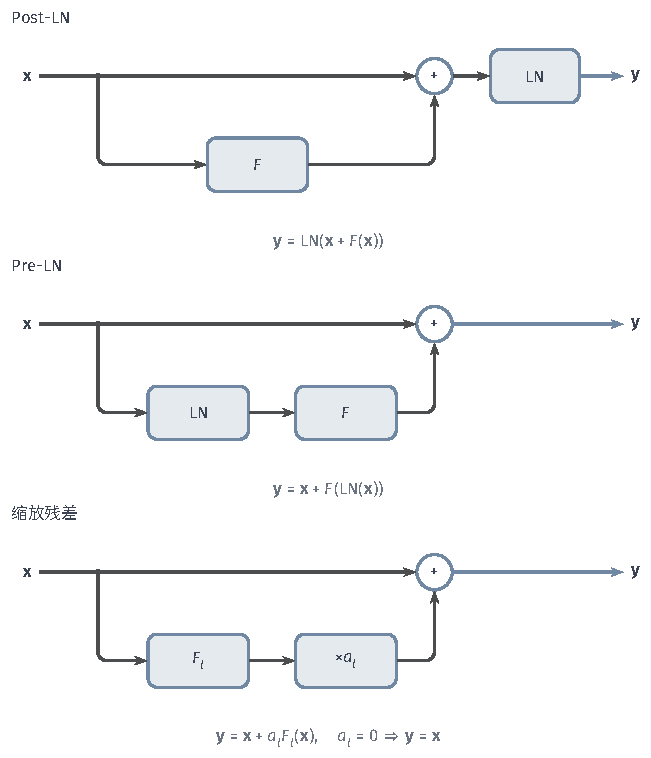
\includegraphics[width=110.225mm]{figures/03-models/02-neural-network-models/tikz/transformer-residual-extensions/figure.pdf}
  \caption{把恒等路径放在同一水平线上比较三种残差组织。Post-LN的原输入在相加后仍通过LN；Pre-LN只有下方变换支路经过LN，恒等路径可以直接到达输出。第三行以$a_l$缩放新增变换，$a_l=0$时该子层输出等于输入；ReZero采用这一初值，图中省略可选归一化。各行上方路径传递原表示，下方路径计算新增变换，$+$为逐元素相加。}
  \label{fig:transformer-residual-extensions}
\end{figure}
\FloatBarrier

\subsection{混合网络结构}
\label{sec:transformer-hybrid}

稠密注意力保存位置表示并显式读取它们。局部窗口与固定容量历史状态可以由其他模块提供，与这份逐位置存储组合。若输入具有稳定局部模式，可以用卷积前端提取特征、降低分辨率，再把特征位置送入Transformer；窗口内部的卷积共享与注意力的内容相关读取承担不同职责。下采样减少序列长度，会明显改变后续平方位置对成本，也可能丢失细粒度信息，输出任务需要保留或恢复相应分辨率。

模块也可以交替堆叠。例如用状态空间模块压缩历史，用注意力层在保留位置之间进行显式检索；或者先用循环网络处理陆续到达的观测，再在给定窗口内交换信息。串联改变后一个模块接收到的表示，前端压缩决定后续可用内容，细节若没有保存在输出或旁路中，注意力就只读取剩下的表示。并行分支则可以分别形成局部与全局表示，再相加或拼接，维度、位置对齐和因果规则仍需一致。

各模块的成本沿实际执行累加：只要保留稠密注意力层，整段处理仍有平方量级的位置对计算；生成时，该层需保存随历史长度线性增长的KV缓存。训练中间存储另取决于实现，FlashAttention不必保存完整的平方规模注意力矩阵；固定状态节省相应模块的历史存储，保留的注意力层仍需自己的键值。前端、交替与并行是不同组织方式，应围绕任务需要的局部模式、精确历史读取、延迟和计算预算选择。

图~\ref{fig:transformer-hybrid}比较前端、交替与并行三种组织。它们分别改变输入粒度、层间分工与融合方式，使用哪一种都需要保持位置对应和信息可见规则。

\begin{figure*}[htbp]
  \centering
  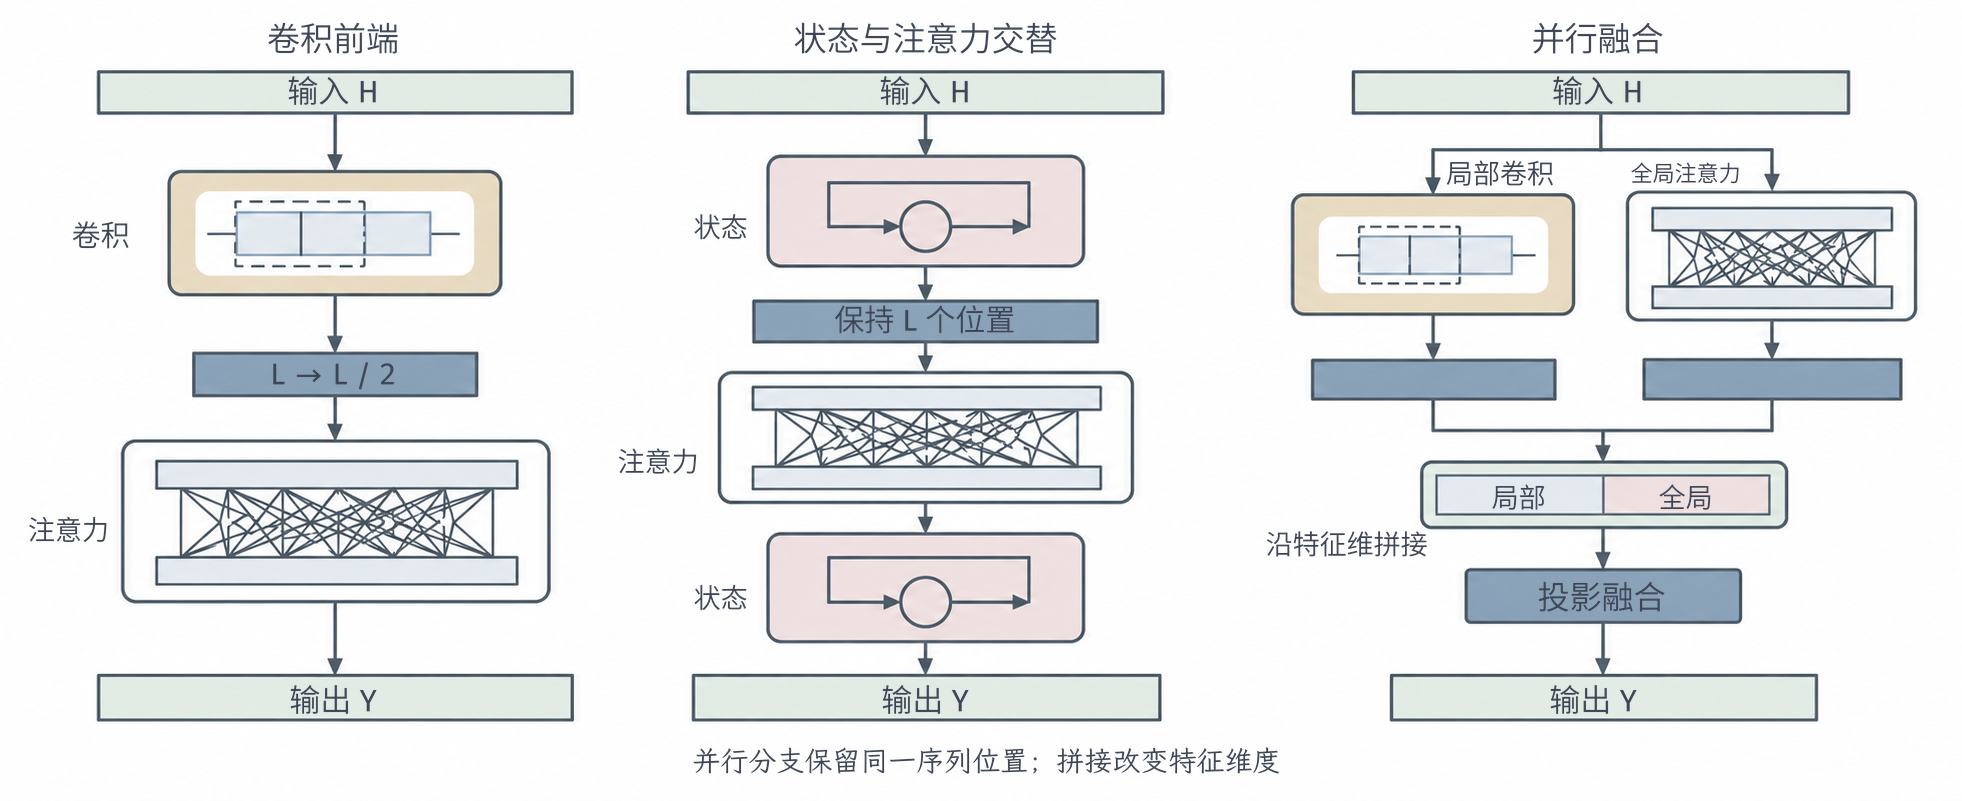
\includegraphics[width=166.116mm]{figures/03-models/02-neural-network-models/generated/transformer-hybrid/figure.png}
  \caption{三种混合结构改变的是不同环节。左图在$L$为偶数、无填充的设置下，以窗口2、步长2的卷积前端将$L$个输入位置变成$L/2$个特征位置，再交给注意力；中图沿输入位置递推状态，并将各位置输出交给注意力层，随后继续交替；右图对同一序列并行计算局部卷积和注意力，拼接框沿特征维合并两路表示，再经投影融合。并行分支采用保持长度的位置对齐设置，所有分支还需满足任务的因果约束。}
  \label{fig:transformer-hybrid}
\end{figure*}
\FloatBarrier

\section{理论分析}
\label{sec:transformer-theory}

一个位置可以读取哪些信息，决定目标是否可能由这些表示实现；参数怎样更新，决定训练能否找到有用的候选；训练样本之外的输入，又检验所得规则能否复用。下面按表达能力、收敛性和泛化性讨论这三个问题，把注意力尺度、归一化、长度及结构约束放入各自条件。

\subsection{表达能力}
\label{sec:transformer-expressivity}

注意力让一个位置读取允许集合中的其他位置，多头与FFN进一步组合这些结果。候选空间是否包含目标，取决于可见性、位置表示、宽度、深度和读出。没有位置或其他顺序线索的自注意力保持置换等变性，因而不能单靠内容判断相同词元排列的先后；因果模型只能使用前缀；需要完整后文的逐位置目标则要提供相应可见上下文。

固定最大长度规定了候选函数的输入范围；长度继续增长时，所需传播、状态和读出也可能改变。有限层读取虽能跨越远距离，却仍要在有限维状态中选择、组合并保留所需信息。稀疏连接、低秩压缩和共享键值改变候选自由度，可能适合目标，也可能遗漏关键交互；目标所需交互决定这些约束是否合适，表示成本再据实际路径计算。

\subsection{收敛性}
\label{sec:transformer-convergence}

Softmax的Jacobian矩阵$\bm J=\operatorname{diag}(\bm a)-\bm a\bm a^{\top}$的谱范数不超过$1/2$。可由每行绝对值之和$2a_j(1-a_j)\leq1/2$以及对称性得到这一界。它控制的是对得分的局部敏感度；当权重接近单点时，Jacobian矩阵还可能趋近零。因此，Softmax对得分的局部增益有界，权重趋近单点时的饱和还会削弱评分梯度。

注意力对输入的敏感度还包含查询、键和值的变化。单头记$\bm Z=\bm A\bm V$，固定掩码时微分为
\begin{equation}
  \begin{aligned}
    \mathrm d\bm Z&=(\mathrm d\bm A)\bm V+\bm A\,\mathrm d\bm V,\\
    \mathrm d\bm S&=\frac{(\mathrm d\bm Q)\bm K^{\top}
                              +\bm Q(\mathrm d\bm K)^{\top}}{\sqrt{d_k}}\text{。}
  \end{aligned}
  \label{eq:transformer-attention-differential}
\end{equation}
结合逐行Softmax界和矩阵范数不等式，可得局部估计
\begin{equation}
  \begin{aligned}
    \lVert\mathrm d\bm Z\rVert_{\mathrm F}
    &\leq\frac{\lVert\bm V\rVert_2}{2\sqrt{d_k}}
       \left(\lVert\bm K\rVert_2\lVert\mathrm d\bm Q\rVert_{\mathrm F}
             +\lVert\bm Q\rVert_2\lVert\mathrm d\bm K\rVert_{\mathrm F}\right)\\
    &\quad+\lVert\bm A\rVert_2\lVert\mathrm d\bm V\rVert_{\mathrm F}\text{，}
  \end{aligned}
  \label{eq:transformer-attention-local-bound}
\end{equation}
其中矩阵$\lVert\cdot\rVert_2$为谱范数，$\lVert\cdot\rVert_{\mathrm F}$为Frobenius范数。输入到投影的敏感度还乘以各$\bm W$的范数。每行是值的凸组合，但多行可以重复读取同一个值，所以一般未必有$\lVert\bm A\rVert_2\leq1$：所有查询都读取同一个值时，该值的影响会在多行重复，谱范数可以达到$\sqrt n$。最大行向量范数逐行测量放大，谱范数测量整份矩阵，两种尺度可能具有不同长度因子。

归一化的分母含$\varepsilon$，其局部导数还受可学习缩放和行内方差影响。残差堆叠则包含多个$\bm I+\bm J_l$的乘积，即使直接路径存在，其他分支仍可能累积放大、衰减或抵消。Pre-LN、残差缩放和门控改变这一乘积，完整乘积的奇异值仍由各分支导数及其组合决定。深度增加、输入长度变长或投影尺度改变，都可能使原来合理的学习率不再适合。

把这些局部因素转为优化结论，需要明确经验目标和轨迹条件。令$J(\bm\theta)$为确定性的全批量经验目标，假定它有下界$J_{\inf}$，并在包含迭代点及更新线段的区域内具有$\beta$-Lipschitz梯度。对固定学习率$0<\eta\leq1/\beta$的完整梯度下降，下降引理给出
\begin{equation}
  \begin{aligned}
    J(\bm\theta^{(t+1)})
      &\leq J(\bm\theta^{(t)})-\frac\eta2
                   \lVert\nabla J(\bm\theta^{(t)})\rVert_2^2,\\
    \min_{0\leq t<T}\lVert\nabla J(\bm\theta^{(t)})\rVert_2^2
      &\leq\frac{2(J(\bm\theta^{(0)})-J_{\inf})}{\eta T}\text{。}
  \end{aligned}
  \label{eq:transformer-stationary-convergence}
\end{equation}
第二行来自第一行求和。它控制前若干个迭代点中最小的梯度范数平方，评价训练接近驻点的程度。参数极限、全局目标差和训练误差还需要相应条件。对有界参数、固定最大长度、光滑激活和正归一化分母的网络，可以在适当紧区域控制光滑常数；ReLU拐点、专家的离散选择、随机Dropout和缓存近似改变了光滑性或实际更新，分析需据这些计算重新规定条件。

要进一步保证目标差距下降，例如需要沿轨迹满足$\lVert\nabla J\rVert_2^2\geq2\mu(J-J_*)$的Polyak--Łojasiewicz条件，其中$\mu>0$且$J_*$为所比较的最优值，才可由上式得到几何下降。该条件把目标差与梯度大小联系起来，能否成立取决于当前目标及训练轨迹。
固定核附近的训练分析还依赖宽度、初始化和核特征值，并限定训练期间核的变化范围。这些条件规定了所分析的网络与优化轨迹（参考\BookTheoremRef{thm:ntk-training-convergence}{第二卷“基础、理论和可信性”的“深度学习的可学习性”章“固定NTK下的训练收敛”定理}）。

随机梯度的结论另需无偏性、方差和步长条件；Adam类自适应更新也有不同的假设。平稳损失曲线描述已观察的数值行为，驻点速率描述梯度尺度，较小训练误差描述拟合结果。最后一项还要求候选与数据相容，并且更新找到相应参数；三个评价量各有自己的条件。

\subsection{泛化性}
\label{sec:transformer-model-generalization}

以序列分类为例，一个样本$z=(x,y)$包含完整输入序列和标签。若训练集$S=\{z_1,\ldots,z_N\}$由同一分布独立抽取，期望风险为$R(f)=\mathbb E\ell(f(x),y)$，经验风险为$\widehat R_S(f)=N^{-1}\sum_{j=1}^N\ell(f(x_j),y_j)$。这里$N$计独立序列，$n$计一条序列的位置。总共$Nn$个词元可以在序列内部相关；把它们按$Nn$个独立样本分析需要另外建立抽样条件。

在抽样前固定模型族$\mathcal F$、允许长度和损失范围，令$\mathcal G=\{z\mapsto\ell(f(x),y):f\in\mathcal F\}$，若损失取值于$[0,1]$且满足可测性条件，以至少$1-\delta$的概率，所有候选的期望风险同时受到经验风险与损失函数族复杂度的控制：
\begin{equation}
  R(f)\leq\widehat R_S(f)+2\widehat{\mathfrak R}_S(\mathcal G)
       +3\sqrt{\frac{\log(2/\delta)}{2N}}\text{。}
  \label{eq:transformer-generalization-bound}
\end{equation}
该界来自有界损失下的Rademacher一致风险分析（参考\BookTheoremRef{thm:rademacher-risk-bound}{第二卷“基础、理论和可信性”的“二分类学习的可学习性”章“Rademacher复杂度给出的期望风险上界”定理}）。它通过损失函数族刻画Transformer；输入范围、投影范数、层数、头数和读出方式共同影响相应复杂度。交叉熵一般无界，超出此处$[0,1]$损失条件；概率下界和适当尺度处理可以建立有界范围，其他用法则需要相应无界损失理论。上界刻画这些条件对风险的控制，较松的数值与实际测试错误率可有较大差距。

\subsubsection{输入与数据}

序列长度同时改变可见证据、计算图规模和数据分布。若每行输入范数不超过$b$，整个矩阵Frobenius范数仍可能达到$\sqrt n\,b$；位置表示的尺度也要计入。第\ref{eq:transformer-attention-local-bound}式说明，谱范数分析可能把这些长度因素带入敏感度和复杂度。另一方面，长度变长也可能提供更多有用信息，界中的$n$因子描述所用范数估计，任务风险还受新增证据及实际预测影响。

样本量需要与依赖结构匹配。独立文档可以作为样本，而同一连续记录中的重叠窗口、同一用户的多段文本或同一图像的多个块可能相关；数据划分和风险定义应反映这些关系。输入尺度过大、词元频率变化、噪声位置增加或训练与测试长度分布不同，都会改变预测器实际遇到的条件。两个位置有直接通路时，训练仍需提供足以学会任务关系的样本或先验。

\subsubsection{参数与学习过程}

查询键范数控制得分尺度，值与输出投影范数控制读取结果，前馈层和归一化缩放影响后续敏感度。参数数目描述可独立调整的系数，同一投影在多个位置复用，因此参数量本身不随$n$成倍增加。执行次数、聚合范围和长度分布继续影响实际计算与风险分析。控制参数范数、分类间隔或适合任务的有效自由度，可以提供比总参数数目更有条件的描述。

训练算法还决定实际选择了哪个参数。正则化、停止时间和步长会改变样本替换对输出的影响；若能证明一致稳定性系数为$\epsilon_{\mathrm{stab}}$，便可据此控制期望泛化间隙（参考\BookTheoremRef{thm:stability-expected-generalization}{第二卷“基础、理论和可信性”的“一般学习的可学习性”章“均匀稳定性与期望风险”定理}）。建立这一系数需要控制样本替换时的注意力、归一化与优化轨迹变化。反复使用验证集选择配置时，评价对象还包含这一选择过程，其数据使用需在分析中保留。

\subsubsection{网络结构与外推边界}

深度提供多轮交互和变换，宽度和头数改变可保留的特征、评分及聚合形式；固定总宽度时，更多头同时减少每头宽度。稀疏连接减少允许的交互，门控和专家路由增加条件计算自由度，位置编码引入顺序与距离规律。这些设计可能与数据结构相匹配，也可能排除任务需要的函数。限制函数族可以降低某些复杂度，却可能提高逼近误差，需要同时考虑。

\term{同分布泛化}（in-distribution generalization）要求新样本来自训练所对应的分布；\term{长度外推}（length extrapolation）要求在训练未覆盖的更长输入上复用规则；\term{分布外泛化}（out-of-distribution generalization）则改变输入或任务条件。相同长度同分布的新文本检验一类风险；更长输入和新领域改变评估条件，需要各自检验规则复用与可靠性。

固定正弦、ALiBi和RoPE提供可用于新位置的计算规律，长度外推还涉及内容分布、距离分布、聚合稀释、层数是否足够及读出规则。因果掩码保证前缀可见范围，长文本的语义一致性则由状态表示、训练目标及实际生成检验。跨任务学习与长度外推还需重新规定任务、目标分布和预测过程（参考\BookSectionRef{sec:learning-theory-research-content}{第二卷“基础、理论和可信性”的“机器学习理论基础”章“研究内容”节}）。本章的结构比较提供相应分析所需的计算对象。

\section{常见应用}
\label{sec:transformer-applications}

应用中的完整模型需要把输入单位、可见信息、输出含义和监督位置对应起来。以下沿用前文的网络块与损失，只展开从样本到预测的路径；数据构建、任务专用结构与评价方法由应用卷细化。

\subsection{文本分类与序列标注}
\label{sec:transformer-text-applications}

评论情感分类的样本是文本和类别。分词后查表形成嵌入，加位置表示，使用双向编码器得到上下文表示，再采用CLS或掩码池化读出，经Softmax分类。以“这部电影并不精彩”为例，编码器给“精彩”的表示可以读取否定上下文，整段分类头据此输出类别。否定关系提供这项任务需要的证据，模型通过哪些头和特征使用它，可以结合响应分析；最终预测由独立样本评价。

训练对评论计算交叉熵，嵌入、编码器和分类头共同更新；如果先使用已有模型，再训练任务头或微调部分层，需要明确哪些参数更新。推理使用同一分词与有效位置规则，输出整段概率。截断删去的文本可能包含判断证据，训练和测试的长度处理因而共同规定实际预测条件。

实体标注则将每个有效位置表示送入共享分类头，计算对应标签损失。若一个词被拆成多个子词，标签需选择监督首个子词、监督所有子词，或先聚合为词表示，推理时也用同一规则。逐位置Softmax分别形成标签概率，跨位置标签组合若有约束，还需由相应输出模型联合处理。离线标注读取整段，流式标注使用因果或有限延迟范围，这个约束比“采用编码器还是解码器”的名称更直接。

\subsection{序列转换与生成}
\label{sec:transformer-generation-applications}

机器翻译训练使用源句$x$和包含EOS的目标$y$。源嵌入和编码器产生$\bm H_{\mathrm s}$，目标输入右移，因果自注意力读取真实目标前缀，交叉注意力读取有效源位置，以式\eqref{eq:transformer-conditional-loss}更新两侧嵌入、所有网络块和词表输出层。源词和目标词通过条件似然共同训练，注意力权重由这份翻译监督学习软对应。

推理时源端只编码一次，各目标层还可预先缓存该层交叉注意力的源键值。目标从BOS开始，每次前向为当前输入计算并追加各层自注意力键值，再由词表头产生下一词元分布。选出的词元作为下一次输入，逐步延长缓存，遇到EOS或长度上限停止。不同层的投影参数不同，因此源交叉键值与目标自注意力键值都按层保存。束搜索存在多个候选前缀时，可以共享未变的缓存内容，分叉后的修改则需各自维护或按写入时复制处理。

文本续写不需要独立源编码器。已给定提示先做预填充，末位置输出预测提示后的第一个词元；把选出的词元作为新输入，在各层追加缓存，得到下一词元分布。续写读取已经产生的完整前缀，训练则读取真实前缀；两种输入来源决定模型实际经历的上下文。选择温度、采样或搜索策略会影响输出，评价需使用实际采用的生成过程。

\subsection{图像分类}
\label{sec:transformer-vision-applications}

图像具有二维网格位置，将小块编号并投影后，也可以组织为注意力读取的序列。\term{视觉Transformer}（Vision Transformer, ViT）将图像分成块，分别嵌入后进行位置间注意力，再读出图像类别\scite{dosovitskiy2020vit}

设图像高宽为$H,W$、通道数为$c$，块边长为$p$，并暂设$H,W$可被$p$整除，则块数为$n=HW/p^2$，每块展平向量$\bm x_i\in\mathbb R^{p^2c}$。投影后的输入为
\begin{equation}
  \bm h_i^{(0)}=\bm W_{\mathrm p}^{\top}\bm x_i+\bm b_{\mathrm p}+\bm p_i,
  \qquad \bm W_{\mathrm p}\in\mathbb R^{p^2c\times d}\text{。}
  \label{eq:transformer-vit-input}
\end{equation}
位置索引按固定网格顺序排列，位置表示须保留块与空间位置的对应。加入专用分类位置后，共有$n+1$行表示，经编码器、末端归一化和分类头产生概率，以图像标签交叉熵训练。图~\ref{fig:transformer-vit}把图像块、序列表示与分类输出连接起来。

\begin{figure*}[htbp]
  \centering
  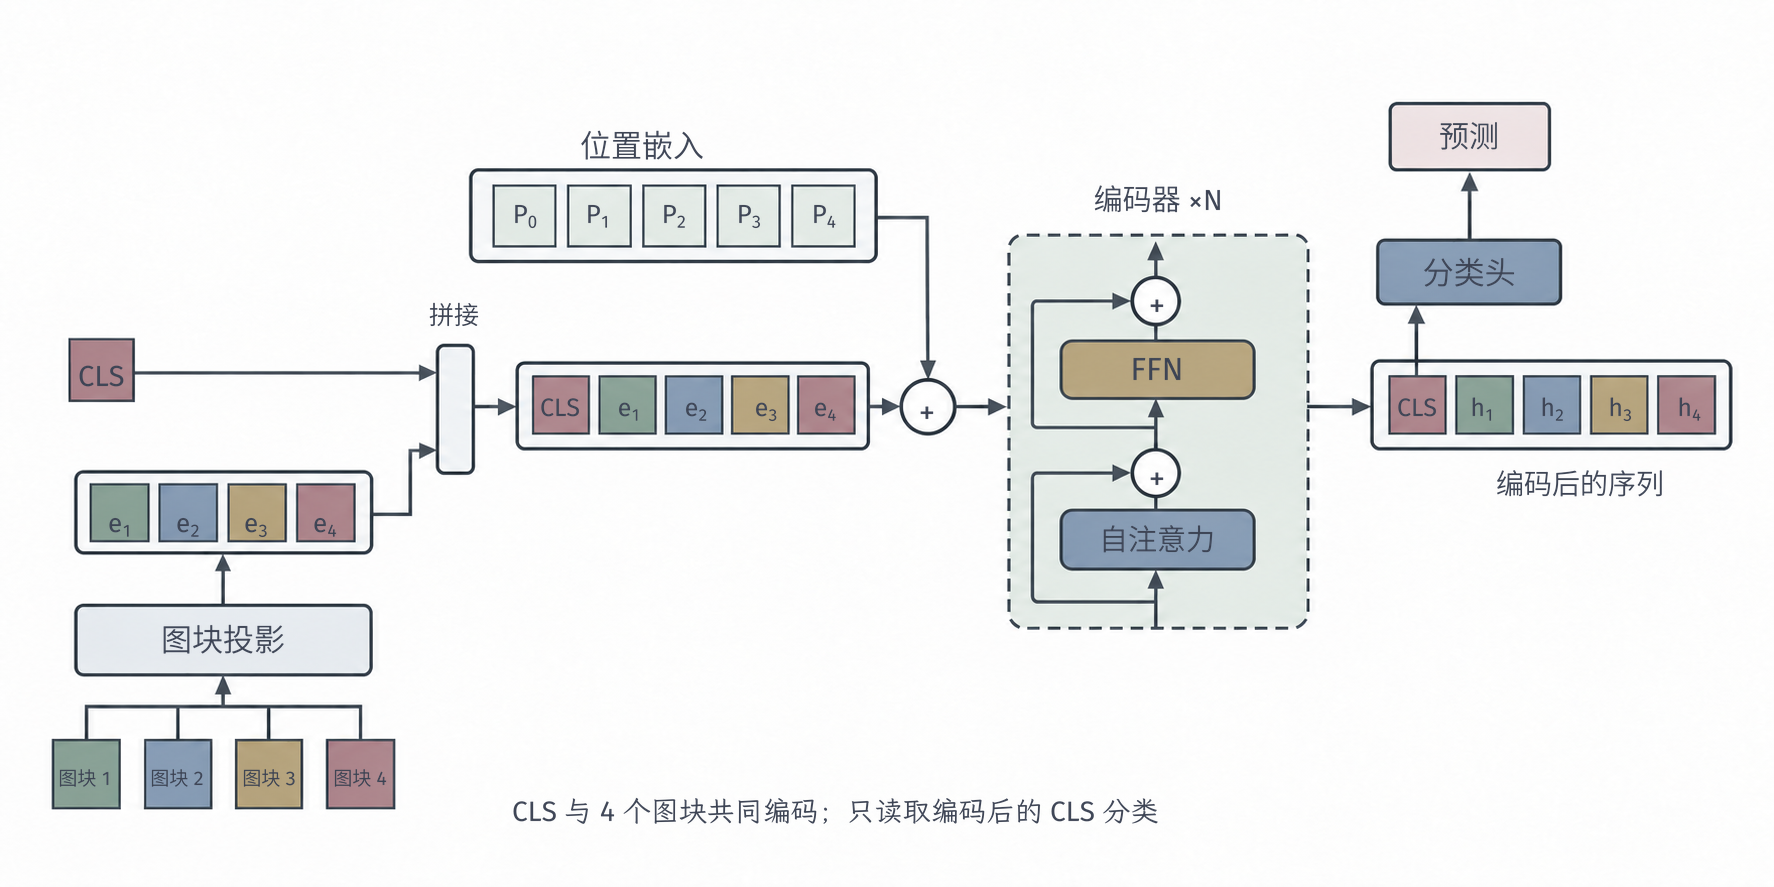
\includegraphics[width=150.199mm]{figures/03-models/02-neural-network-models/generated/transformer-vit/figure.png}
  \caption{ViT将图像组织为序列的过程。四个示意图像块按固定空间顺序编号；每块展平后通过同一线性投影形成$\bm e_i$。在开头加入可学习CLS表示，为五行分别加入位置向量，再送入双向编码器。分类头只读取末层CLS行，其他图像块通过注意力参与其形成。图像块色块仅为结构示意，不声明实际像素尺寸，也不是识别实验样本。}
  \label{fig:transformer-vit}
\end{figure*}
\FloatBarrier

图像块之间可直接交互，但块内部结构在原始ViT中经一次线性投影进入表示，没有逐层卷积的局部共享假设。较小的$p$保留更细的位置划分，同时使$n$增长；固定图像尺寸时，稠密注意力位置对数与$p^{-4}$同阶，前馈层的块数成本则与$p^{-2}$同阶。改变图像分辨率会改变网格和位置数量，可学习位置表常需按空间网格插值；插值提供新网格的位置向量，分类质量还取决于新增图像细节与已学规则的匹配。数据量、预训练、局部模块和增强会影响实际效果，ViT与卷积模型的实际比较需要固定数据、训练投入和评价目标，局部归纳假设与预训练知识共同影响结果。

\Needspace{125mm}
\section{本章小结}
\label{sec:transformer-summary}

Transformer把序列中的位置依赖转为显式读取：内容表示给出查询、键和值，位置表示和掩码约束怎样匹配以及哪些位置可见，多头注意力形成不同聚合，逐位置前馈网络再组合这些特征。残差和归一化让这套计算能够层层堆叠。与循环注意力相比，它可以同时更新已知位置。逐步生成时，新的输出依次成为后续条件，缓存保存已完成的位置计算以便复用。

结构与资源的选择需要同时看任务。双向读取适合完整输入理解，因果读取满足在线与生成条件，交叉注意力将源目标表示分开。位置扩展提供不同距离规律，门控和专家改变特征选择；稀疏、线性和低秩路线改变读取结构或公式，FlashAttention保留稠密计算而减少中间访存，MQA/GQA缩小键值组数，PagedAttention改善缓存分配与共享。减少哪一种开销、改变哪一种表示自由度，决定了这些方法的组合与取舍。

损失沿值读取、评分、特征变换及直接残差路径汇集为参数梯度，训练进展与预测风险再据各自条件评价。得分尺度、归一化分母、残差深度和长度共同影响学习，独立样本数、参数约束、数据分布和评价目标共同约束风险结论。由此可以回答章首的问题：直接位置交互使已知输入的计算更易并行，但可靠预测还取决于可见范围是否正确、任务信息是否保留，以及学习结果是否在实际使用条件下得到检验。

\paragraph{扩展阅读}
Vaswani等的原论文给出编码器与解码器的计算，BERT和GPT-3论文展示不同读取范围及监督方式。公开论文中的归一化、掩码和目标可以与本章公式对照；后续产品的接口能力则按发布资料对应的系统层级理解\scite{vaswani2017,devlin2019,brown2020}

\chapter{脉冲神经网络}
\label{chap:spiking-networks}

一个只报告亮度变化的传感器会不断送来事件：哪个位置发生变化，变化何时到达。把这些事件立即汇总成一个实数向量，可能丢掉两次变化的先后；每隔一段时间处理完整图像，又会反复计算未变化的部分。怎样直接使用到达事件，同时保留强度、顺序和历史？信号的次数、到达时刻及间隔中的内部状态都需要进入模型。

生物神经元以发放事件通信，液态状态机也已经用固定脉冲储备池形成动态，再训练读出（见第\ref{chap:neural-network-overview}章与第\ref{chap:recurrent-networks}章）。如果还要学习多层连接，就需把输出误差接回这些事件和状态。输入怎样编码，内部怎样积累，连接怎样传播，决定这种通信能完成什么预测；时间模拟与训练则产生相应成本。

单元传出的是脉冲，单元内部保留的是膜电位等状态。事件到达时改变状态，两次事件之间的状态继续演化，因而历史可以影响后续响应。本章以离散时间计算连接输入、状态、学习和读出，再用这条完整路径解释事件稀疏性何时有助于节省计算；连续时间方程提供动态来源。

\section{脉冲神经网络概述}
\label{sec:snn-overview}

\subsection{提出动机与核心思想}
\label{sec:snn-motivation}

生物细胞的膜电位连续变化，远距离通信却主要通过短暂的动作电位完成。把活动概括为一个实数激活，会省略单次发放时刻、事件间隔和阈值以下的积累。神经计算研究需要解释这些量怎样影响响应；变化驱动的传感器则直接提供了带时刻的观测。

\term{脉冲神经网络}（spiking neural network, SNN）以离散发放事件在单元之间传递信息，单元内部保存随时间演化的状态。一个脉冲通常只报告某单元在某时刻发放；信号的强度和时序关系由发放次数、发生时刻及发放单元共同承载。接收单元积累这些输入，旧输入逐渐衰减，状态越过阈值时再产生新事件。事件序列承担编码，阈值、复位与状态递推形成处理这些序列的网络。

这种模型服务于两类问题。神经科学需要用动态解释细胞的输入响应，以及局部连接怎样形成行为；工程则希望在变化稀疏时，按到达事件传递和处理信息，减少持续感知中的操作。后一收益取决于完整链路：传感器与编码产生多少事件，网络访问多少连接，设备又怎样更新状态。0与1的通信变量本身没有给出这些成本。

人工任务可以使用只保留积累、泄漏、阈值和复位的简化单元，通过任务损失学习权重，再用连续值读出形成预测。保留哪些细胞机制由研究问题决定：解释发放过程需要相应的生物证据，分类需要任务评价，节省计算则需要检查实际执行的事件与状态更新。

\subsection{从神经元建模到神经形态计算}
\label{sec:snn-early-history}

脉冲网络的发展汇合了神经元动态、时序编码和硬件实现几条路线。它们分别解释事件怎样产生、时间怎样承载信息，以及事件怎样被执行。1907年Lapicque的积分发放思想将输入电流的积累与阈值发放联系起来，是早期简化动态模型的一条路线\scite{gerstner2014}

1952年Hodgkin与Huxley从离子电流出发建立动作电位的定量模型。与积分发放模型相比，它解释波形产生机制，说明神经元模型可以在不同生物细节层次上工作：简化模型便于组织较大网络，细致模型则服务于膜电流和发放机制研究\scite{hodgkin1952membrane}

1990年，Mead系统讨论\term{神经形态电子系统}（neuromorphic electronic systems），即借鉴神经系统组织与动态来设计电子计算系统。它关注的不仅是某个神经元方程，还包括局部连接、并行动态和物理实现；神经形态计算的范围因此比某一种SNN模型更广\scite{mead1990neuromorphic}

1997年，Maass以“第三代神经网络模型”讨论脉冲单元的计算能力，把发放时间明确纳入计算。这一代际划分比较阈值单元、连续激活与脉冲时序能够完成的计算。相应表达结论限定了编码和单元模型；实际任务精度与设备能耗还由训练、数据和执行方式决定\scite{maass1997spiking}

脉冲储备池进一步展示了利用复杂动态而不训练全部循环连接的路线。2002年的液态状态机让输入扰动一个固定循环系统，再训练读出使用其动态状态；第\ref{sec:rnn-lsm}节已给出这种分工。局部可塑性则从突触两端活动出发调整连接，为无需完整反向传播的学习提供另一条路径。储备池把可训练部分放在读出，局部规则把可用信号限制到突触附近；多层监督任务还需要把最终误差分配到更早的事件和连接。

\subsection{深层网络与训练方法的发展}
\label{sec:snn-learning-history}

当目标从解释局部动态转为学习多层分类器，离散阈值成为主要困难。2002年，Bohte等提出SpikeProp，根据发放时刻与目标时刻之间的误差进行反向计算；它对发放时刻求导，所需的模型与发放条件限定了这种时间误差回传的用法\scite{bohte2002spikeprop}

后来的两条路线让深度学习经验更容易进入SNN。一条先训练连续值网络，再校准权重和阈值，使脉冲统计近似原激活；另一条在前向保留离散发放，在反向指定替代导数，直接优化任务损失。第\ref{sec:snn-learning}节会分别说明转换误差和替代梯度的近似性质。2019年的替代梯度综述系统整理了后一条路线，替代规则为不连续发放提供了指定的反向信号，前向阈值仍然保留\scite{neftci2019surrogate}

可训练性改善后，研究开始扩展深度与信息交互方式。2021年的SEW-ResNet研究怎样在脉冲残差路径中保持合适的传播；2022年发布、2023年发表于ICLR的Spikformer则将脉冲形式的查询、键和值用于注意力计算。残差组织层间传播，注意力组织信息读取；其中连续运算、时间步使用和硬件映射方式又分别影响训练与执行成本\scite{fang2021spikingresnet}

Spikformer将两种约定组合起来：事件编码与神经元动态规定单元怎样响应，注意力与层间组织规定怎样读取信息。具体模块需要相应的脉冲实现；静态图像还需编码成多步输入，其事件数由这份编码与网络响应决定\scite{zhou2023spikformer}

\subsection{与连续值神经网络的比较}
\label{sec:snn-ann-comparison}

两类网络都可以有前馈、卷积、循环或注意力连接，区别主要在单元输出与时间动态。普通前馈单元一次产生实数激活；脉冲单元先更新内部状态，再决定是否发放。第\ref{sec:rnn-lsm}节的漏积分发放（leaky integrate-and-fire, LIF）单元即使没有循环边，也能用膜电位保存过去输入的影响，而普通逐帧前馈网络通常没有跨帧状态。RNN同样保存跨时间状态；与它相比，SNN的特殊之处在于明确的发放、复位和事件通信。

一个比特可以作为二值网络的层输出，也可以表示某时间区间内有没有发放。后一含义与内部状态相连：SNN输出0时，过去输入仍可能留在膜电位中，后来事件会接着这份积累进入计算。表~\ref{tab:snn-ann-comparison}比较通信、状态、时间与读出怎样共同形成预测。
\begin{table*}[htbp]
  \centering\small
  \begin{tabularx}{\linewidth}{@{}p{25mm}XX@{}}
    \toprule
    比较维度 & 连续值网络 & 脉冲神经网络 \\
    \midrule
    通信变量 & 实数激活或向量 & 发放事件；数量与时刻共同承载信息 \\
    单元内部状态 & 前馈单元通常无跨输入状态；RNN有状态 & 膜电位、突触响应及可选适应状态 \\
    时间关系 & 由递推、位置或时间特征表达 & 由事件时刻、积累、泄漏与延迟表达 \\
    求导困难 & 常见激活可微或分段可微 & 阈值发放不连续，需特别处理 \\
    训练路线 & 任务梯度及其他学习方法 & 局部规则、时间求导、替代梯度或网络转换 \\
    执行成本 & 取决于算子、稀疏性与设备 & 还取决于观察窗口、事件访问和状态更新 \\
    输出形式 & 分类分数、概率或连续量 & 计数、发放时间或连续状态读出 \\
    \bottomrule
  \end{tabularx}
  \caption{以常见人工模型比较两类网络。连续值网络也能使用稀疏计算、动态状态和局部学习；SNN也可能在通用设备上按固定时间步进行稠密计算。预测质量和能耗需要在相同输入、决策条件与设备设置下另作比较。}
  \label{tab:snn-ann-comparison}
\end{table*}
\FloatBarrier

\subsection{应用现状与发展方向}
\label{sec:snn-development}

事件视觉、稀疏声音或触觉感知、持续监测与机器人响应，是SNN值得研究的场景：输入随时间到达，变化可能稀疏，决策又关心响应延迟。2017年Amir等将事件相机、脉冲识别网络与TrueNorth处理器用于实时手势识别，给出了传感器到设备执行的完整研究系统。这项研究把事件输入、网络响应和设备测量接在同一链路中，结果对应其手势任务、设备与测试条件\scite{amir2017gesture}

硬件的发展提供了更灵活的实验平台。Loihi面向事件通信、神经元状态和片上学习；Loihi 2进一步支持可编程神经元动态。Intel于2024年公布并部署到Sandia的Hala Point，以Loihi 2构成大规模神经形态研究系统。这项交付为研究设施提供了较大规模的事件计算平台，应用范围由设施中的具体实验与工作负载界定\scite{intel2024halapoint}

应用前景取决于完整链路。若输入本来是密集静态图像，需要编码并模拟许多时间步，事件数量和等待时间可能抵消部分收益；若输入是稀疏事件流，输出还需在较短窗口内可靠形成，噪声、低发放量和阈值校准就更关键。分类结果衡量预测，操作量或能耗估计描述成本模型，实际设备测量则反映执行链路；共同的输入与决策条件使这些结果能够相互对应。

已有发展显示两条仍在推进的路线：一条扩大模型的可训练深度、注意力组织和任务范围，另一条围绕稀疏传感器与专用设备共同设计编码、动态和执行方式。深层任务模型与完整实验系统已经提供了可研究的计算对象。数据适配、训练成本、状态存储和软件执行决定这些对象怎样进入其他场景；后面的结构、学习与理论分析将把这些条件落到编码和动态上。

\section{网络结构}
\label{sec:snn-coding-dynamics}

脉冲网络由输入编码、带状态的神经元、突触连接和读出组成。连接决定事件送到哪里，神经元动态决定事件到达后留下什么状态、何时产生下一次发放。输入编码规定事件含义，单元内部的计算规定历史保留；把这些单元接起来，才得到前馈或循环的信息路径。

\subsection{频率编码与时间编码}
\label{sec:snn-coding}

假设一个传感器在一段时间内观察到某种强度。连续值网络可以直接接收这个数，脉冲网络则需要约定如何把它写进事件序列。对第$i$个输入通道，记发放时刻为$t_{i,k}$。连续时间的脉冲列可以形式化为
\begin{equation}
  s_i(t)=\sum_k\delta(t-t_{i,k})\text{，}
  \label{eq:snn-spike-train}
\end{equation}
其中$\delta$为Dirac脉冲，其意义通过积分给出：对一个只包含某次发放的时间区间积分，得到1。这个表示省略了动作电位的波形，只记录事件时刻。计算机模拟常将时间分为宽度$\Delta t$的$K$个区间，令$s_i^{(t)}\in\{0,1\}$表示第$t$个区间是否发放；若同一区间允许多次发放，可以改用计数，后续计算也相应处理这份次数。

\term{频率编码}（rate coding）用观察窗口内的脉冲数量表示输入强弱。若窗口长度为$T_{\mathrm{win}}=K\Delta t$，计数与频率为
\begin{equation}
  N_i=\sum_{t=1}^{K}s_i^{(t)},\qquad
  r_i=\frac{N_i}{T_{\mathrm{win}}}\text{。}
  \label{eq:snn-rate-code}
\end{equation}
因此，同样的脉冲数即使排列不同，也具有相同的窗口频率。将非负输入$x_i\in[0,1]$编码为每个区间独立以概率$x_i$发放，是一种教学上容易分析的随机方案。它满足$\mathbb E[N_i/K]=x_i$，方差为$x_i(1-x_i)/K$。延长窗口可以降低这种抽样误差，但增加等待时间和期望事件数。这里的方差来自独立抽样；相关发放的计数误差还会包含事件之间的协方差。

如果任务要区分“哪个信号先到”，仅统计数量会丢失关键关系。\term{时间编码}（temporal coding）用发放时刻或相对时间关系承载信息。例如，\term{首次发放时间编码}（time-to-first-spike coding）可以约定强输入更早发放，在窗口起点已知时令$t_i=T_{\mathrm{win}}(1-x_i)$。也可以用相邻脉冲间隔或多个单元的相对时序编码。首次发放的含义依赖窗口起点与时间到强度的约定。未发放如何解码、时间怎样量化，以及抖动和起点误差怎样影响恢复值，也属于这份编码。

图~\ref{fig:snn-codes}中的两组事件计数相同、顺序不同。频率读出把它们映射到同一个数；保留时刻的输入则让动态网络获得另一种区分依据。突触、状态和最终读出需要继续保留这份时序差别，它才会进入预测。
\begin{figure}[htbp]
  \centering
  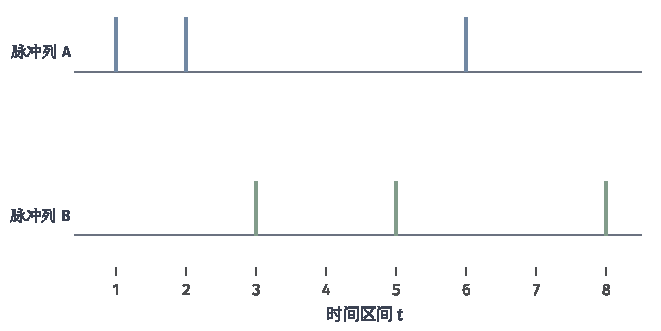
\includegraphics[width=105.412mm]{figures/03-models/02-neural-network-models/matplotlib/snn-codes/figure.pdf}
  \caption{两条构造的脉冲列在8个等宽时间区间内都发放3次，窗口频率相同，但首次发放位置和脉冲间隔不同。竖线表示事件，横轴为时间区间编号；频率读出只保留计数，时间读出还可使用排列。}
  \label{fig:snn-codes}
\end{figure}

输入编码与输出解码不必相同。网络可以接收时间戳事件，再用输出计数分类；也可以接收持续电流，通过输出单元的首次发放作决策。输入到事件、输出到预测的两份约定共同规定了任务接口，相同观察条件下才有共同的精度与延迟口径。

\subsection{积分、泄漏与发放}
\label{sec:snn-neurons}

图~\ref{fig:snn-neuron-structure}将一个单元拆为突触响应、积分与泄漏、阈值检测和复位。输入事件只在到达时写入突触，突触响应与膜电位则保存连续值状态。输出脉冲反馈到复位路径，复位后的电位再经过一个时间步进入下一次积累；这条内部反馈使先前积累可以影响下一次响应，即使单元之间没有循环边。
\begin{figure*}[htbp]
  \centering
  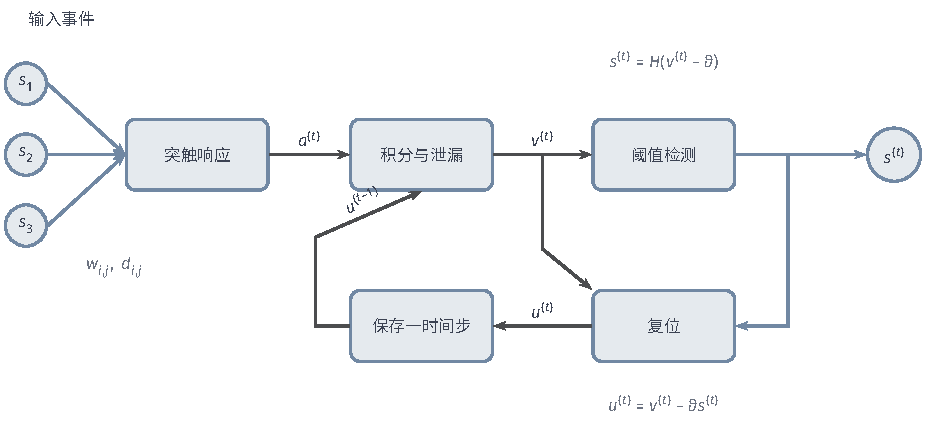
\includegraphics[width=156.792mm]{figures/03-models/02-neural-network-models/tikz/snn-neuron-structure/figure.pdf}
  \caption{离散脉冲神经元的计算结构。输入事件经带权突触形成输入增量$a^{(t)}$，积分与泄漏模块更新复位前电位$v^{(t)}$，阈值检测模块输出脉冲$s^{(t)}$。复位模块计算电位$u^{(t)}$，下方反馈将其保存供下一步使用。图表示本章的更新次序，不表示细胞的解剖结构；突触自身也可保存状态，见式\eqref{eq:snn-synaptic-state}。}
  \label{fig:snn-neuron-structure}
\end{figure*}

一个输入脉冲常不足以触发输出。神经元需要累积输入，同时让旧输入的影响逐渐减弱。\term{膜电位}（membrane potential）是描述这种内部积累的状态变量。在简化人工模型中，膜电位相对于阈值的位置决定是否发放，这份积累还会影响下次响应。

\term{漏积分发放模型}（LIF）在两次发放之间用一阶动态描述积累与遗忘。设膜电位为$u_i(t)$，静息电位为$u_{\mathrm{rest}}$，输入电流为$I_i(t)$，膜时间常数为$\tau_m>0$，电阻为$R$，则
\begin{equation}
  \tau_m\frac{\mathrm d u_i(t)}{\mathrm d t}
  =-[u_i(t)-u_{\mathrm{rest}}]+RI_i(t)\text{。}
  \label{eq:snn-continuous-lif}
\end{equation}
无输入时，偏离静息电位的部分按$\exp(-\Delta t/\tau_m)$衰减。膜电位从下方达到阈值$\vartheta>u_{\mathrm{rest}}$时，模型产生一次脉冲并复位。\term{不应期}（refractory period）指发放后暂时不能再次发放的时间，可通过锁定状态或禁止发放来建模。微分方程描述两次发放之间的变化，阈值检测、复位和不应期再规定事件产生及其后的状态\scite{gerstner2014}

为便于训练，以下把静息电位移到0，并把电流及积分系数吸收到输入增量$a_i^{(t)}$中。采用先积分、再检测、再减去阈值的离散模型：
\begin{align}
  v_i^{(t)}&=\alpha u_i^{(t-1)}+a_i^{(t)},
  &\alpha&=\exp(-\Delta t/\tau_m),\label{eq:snn-discrete-integrate}\\
  s_i^{(t)}&=H(v_i^{(t)}-\vartheta),
  &H(z)&=\begin{cases}1,&z\geq0,\\0,&z<0,\end{cases}
  \label{eq:snn-discrete-fire}\\
  u_i^{(t)}&=v_i^{(t)}-\vartheta s_i^{(t)}\text{。}
  \label{eq:snn-soft-reset}
\end{align}
$v_i^{(t)}$为检测前电位，$u_i^{(t)}$为复位后电位，$\alpha\in(0,1)$控制相邻时间步之间的保留程度。此模型每步最多发放一次。若$v_i^{(t)}$远大于阈值，剩余电位会留到后面；这一单步表示因而无法记录步内可能出现的多次发放。时间步与输入尺度共同决定这项发放上限是否适合任务。

式\eqref{eq:snn-soft-reset}称为减法复位，保留超过阈值的剩余电位。另一种\term{硬复位}（hard reset）直接将发放后的电位设为$u_{\mathrm{reset}}$，即$u_i^{(t)}=(1-s_i^{(t)})v_i^{(t)}+s_i^{(t)}u_{\mathrm{reset}}$。两种复位既改变前向轨迹，也改变反向传播。去掉泄漏、令$\alpha=1$，得到离散的\term{积分发放模型}（integrate-and-fire, IF）；增加适应变量或非线性电位项，可以描述更丰富的发放模式。增加适应或其他动态状态，也增加相应的存储、更新与求导路径。

\begin{example}[相同输入在不同间隔下的结果]
  \label{ex:snn-integration}
  取$\alpha=0.8$、$\vartheta=1$、$u^{(0)}=0$，不设不应期。输入增量$(0.6,0.6,0,0.6)$依次给出检测前电位$(0.6,1.08,0.064,0.6512)$，输出为$(0,1,0,0)$，复位后电位为$(0.6,0.08,0.064,0.6512)$。第二步的两个近邻输入共同越过阈值，第四步到来时，先前积累已经衰减，所得电位仍在阈值下。

  若将相同的三个$0.6$改放在第1、3、5步，中间输入为0，则检测前电位依次为$0.6,0.48,0.984,0.7872,1.22976$，只有第五步发放。总输入不变，输出时刻却改变了。这组教学数值把泄漏与事件间隔的作用落实到可复算的状态轨迹。
\end{example}

图~\ref{fig:snn-lif}把示例的第一组输入画成轨迹。检测前电位用于判断发放，复位后电位成为下一步的初始状态，图中的标记也按这一次序区分。
\begin{figure}[htbp]
  \centering
  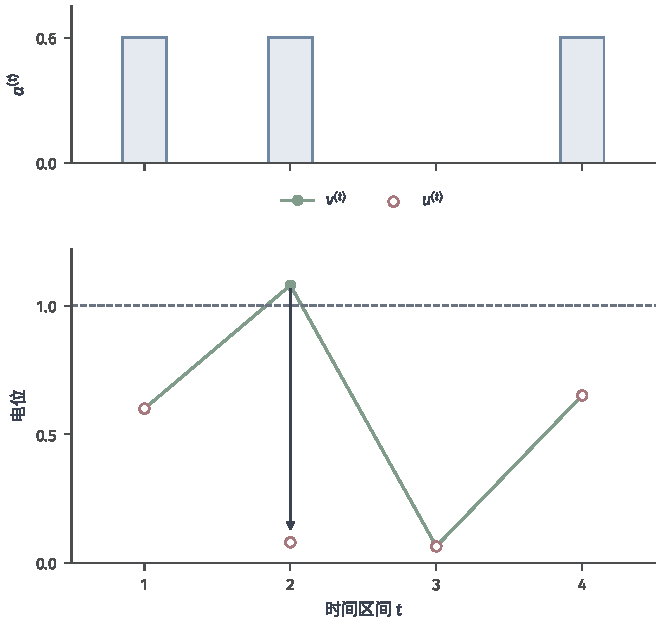
\includegraphics[width=105.412mm]{figures/03-models/02-neural-network-models/matplotlib/snn-lif/figure.pdf}
  \caption{示例~\ref{ex:snn-integration}的离散LIF计算。蓝色柱形表示输入增量，绿色实线连接检测前电位$v^{(t)}$，红色空心圆为复位后电位$u^{(t)}$，虚线为阈值；第二步检测后发放并减去1。连线帮助比较离散状态，不表示步间的连续电位轨迹。}
  \label{fig:snn-lif}
\end{figure}

LIF保留了积累与遗忘，但固定阈值不表达“刚刚频繁发放后变得较难继续发放”。可以增加适应迹$r_i^{(t)}$，例如
\begin{equation}
  r_i^{(t)}=\rho r_i^{(t-1)}+s_i^{(t-1)},\qquad
  \vartheta_i^{(t)}=\vartheta_0+\kappa r_i^{(t)},
  \quad 0\leq\rho<1,\quad\kappa\geq0\text{。}
  \label{eq:snn-adaptive-threshold}
\end{equation}
过去发放暂时抬高阈值，适应迹随后衰减；替换式\eqref{eq:snn-discrete-fire}中的阈值即可形成一种适应LIF模型。额外状态延长动态时间尺度，也增加反向路径和存储。更复杂的神经元可以使用适应电流、非线性膜电位或离子通道状态。例如，\term{自适应指数积分发放}（adaptive exponential integrate-and-fire, AdEx）模型结合膜电位的指数非线性与适应电流。表~\ref{tab:snn-neuron-models}按状态变量与发放机制列出这些模型，使保留的细节与研究问题能够对应。
\begin{table*}[htbp]
  \centering\small
  \begin{tabularx}{\linewidth}{@{}
    >{\raggedright\arraybackslash}p{34mm}
    >{\raggedright\arraybackslash}p{49mm}
    >{\raggedright\arraybackslash}X@{}}
    \toprule
    神经元模型 & 主要状态与发放机制 & 适用关注点 \\
    \midrule
    积分发放（IF） & 膜电位积分，阈值与复位 & 简化计数对应，未包含泄漏 \\
    漏积分发放（LIF） & 膜电位积累与泄漏，阈值与复位 & 有限时间记忆与较低单元复杂度 \\
    适应LIF & 膜电位及适应迹，动态阈值或电流 & 发放历史改变后续响应 \\
    自适应指数积分发放（AdEx） & 膜电位非线性及适应电流 & 以较少状态描述丰富发放模式 \\
    Izhikevich模型 & 膜电位与恢复变量，阈值复位 & 以简化二维动态模拟多种放电行为 \\
    单室Hodgkin--Huxley & 膜电位与离子通道门控变量 & 解释动作电位产生的电流机制 \\
    \bottomrule
  \end{tabularx}
  \caption{神经元模型按保留的动态细节比较。IF与LIF还需规定复位、不应期及时间离散化；表中不计另行添加的突触和延迟状态。增加状态可以描述更多动态细节，任务预测质量则由数据、训练和相应读出评价。}
  \label{tab:snn-neuron-models}
\end{table*}
\FloatBarrier

模型细节由需要解释的响应决定。积累事件形成分类分数可以使用简化状态；研究动作电位波形或离子电流则需要能够产生这些量的动态。不同模型的参数单位、输入尺度与离散步长共同决定实际轨迹，相应数值要在各自方程中解释\scite{gerstner2014}

\subsection{网络连接与状态传播}
\label{sec:snn-connections}

图~\ref{fig:snn-connections}比较相同单元的两种组织。前馈边将事件送到下一层，每个单元的膜电位仍跨时间保留；循环边再把网络过去的发放送回当前计算。层间拓扑决定事件送往哪里，内部状态递推决定事件的影响保留多久，两者可以分别设计。
\begin{figure*}[htbp]
  \centering
  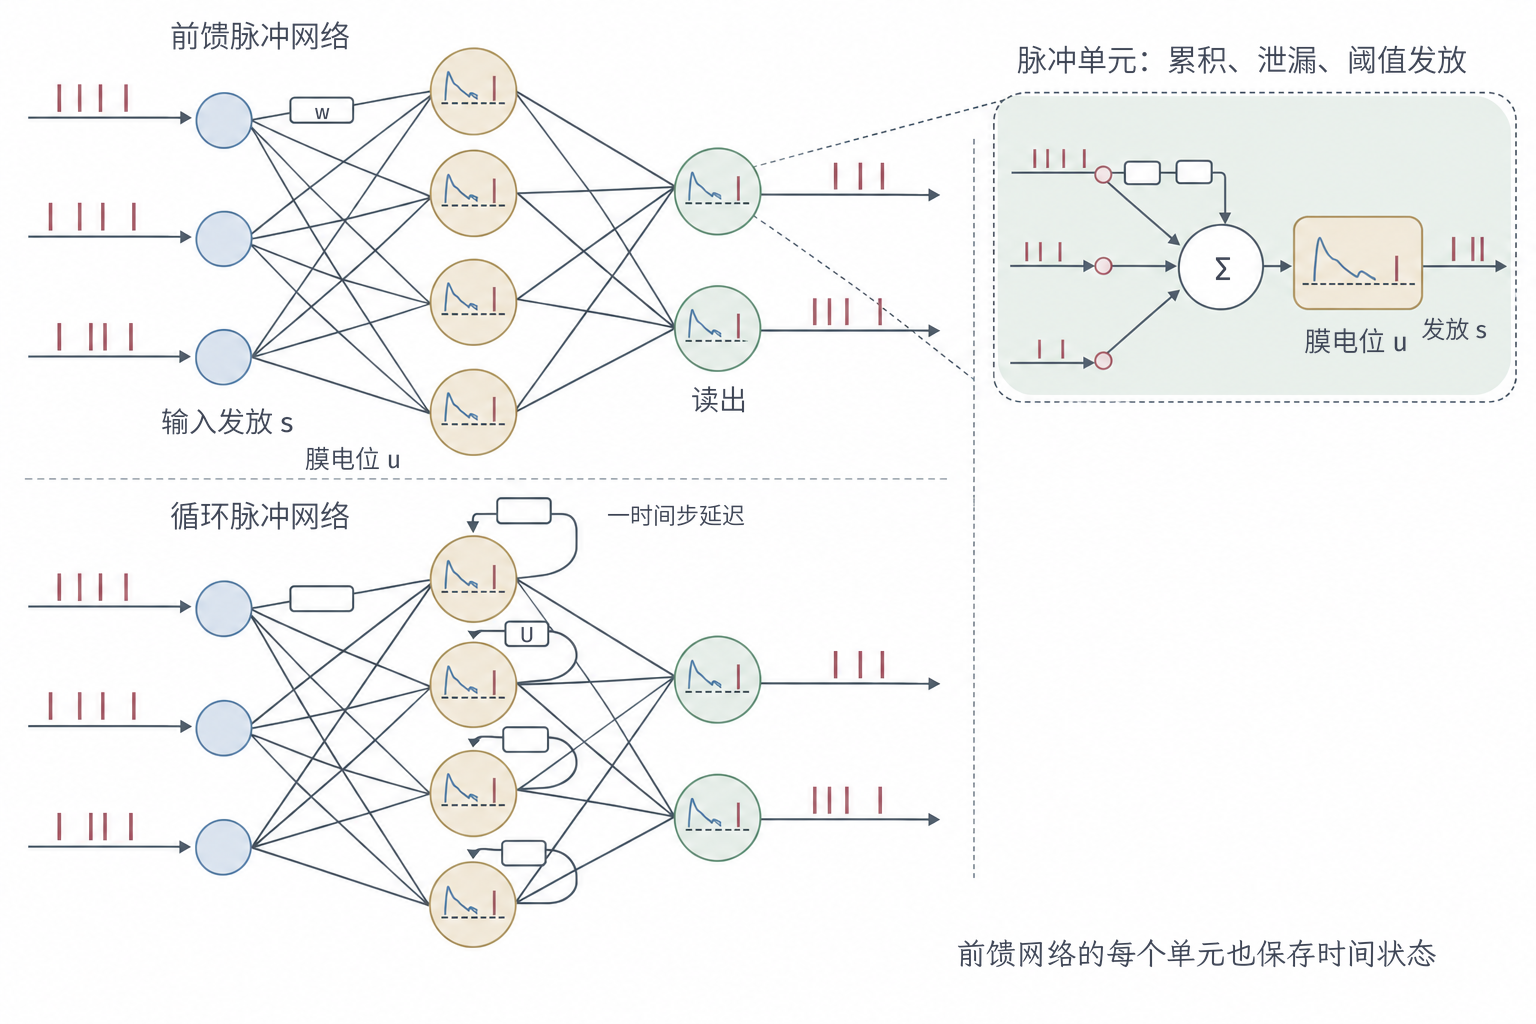
\includegraphics[width=130.048mm]{figures/03-models/02-neural-network-models/generated/snn-connections/figure.png}
  \caption{脉冲前馈网络与循环网络的构造性比较。单元内的膜电位轨迹表示内部状态，箭头传递离散发放，右侧给出输出读出。上半部只保留层间前馈连接；下半部增加使用上一时间步脉冲的循环边$\bm U$。边还可带权重与传播延迟，图中只标出一条代表连接。神经元数和连边用于说明结构，不对应训练模型。}
  \label{fig:snn-connections}
\end{figure*}

神经元之间的连接将发放事件变为后续单元的输入。\term{突触}（synapse）在这里指带权连接及其对接收状态的作用。最简单的离散突触把一个到达脉冲转为电位增量$w_{i,j}$：正权重促使接收单元接近阈值，负权重使其远离阈值。这里的人工模型允许同一单元的输出连接分别取正负权重。生物兴奋性、抑制性细胞对连接符号有更强约束，研究细胞类型时需将这些约束纳入模型。

输入的作用还可以延续多个时间步。设一层有$m$个神经元，上层有$d$个，突触状态为$\bm q^{(t)}\in\mathbb R^m$，前馈权重为$\bm W\in\mathbb R^{m\times d}$，循环权重为$\bm U\in\mathbb R^{m\times m}$，偏置为$\bm b\in\mathbb R^m$，可写为
\begin{equation}
  \bm q^{(t)}=\beta\bm q^{(t-1)}
    +\bm W\bm s_{\mathrm{in}}^{(t)}
    +\bm U\bm s^{(t-1)}+\bm b,\qquad
  \bm a^{(t)}=\bm q^{(t)}\text{，}
  \label{eq:snn-synaptic-state}
\end{equation}
其中$\beta\in[0,1)$控制突触响应的衰减。到达脉冲写入$\bm q^{(t)}$，随后它与$\bm u^{(t)}$按各自衰减率保存历史。循环读取上一时间步的发放，使本步更新有已知输入；前馈层按层次顺序读取本步已经算出的发放。

更一般地，令$d_{i,j}\in\{0,1,2,\ldots\}$表示边$j\to i$的总传播延迟，以离散时间步计，实际延迟为$d_{i,j}\Delta t$。权重为$w_{i,j}$的边贡献$w_{i,j}s_j^{(t-d_{i,j})}$；式\eqref{eq:snn-synaptic-state}中的前馈边对应$d_{i,j}=0$，循环边对应$d_{i,j}=1$。为保持显式更新，每个反馈回路的总延迟必须至少为一步；零延迟边组成的子图必须无环，才能按拓扑顺序读取本步已经算出的脉冲。若允许零延迟自反馈，例如$s=H(2s-1)$，则$s=0$与$s=1$都满足方程，同一历史因而允许两个本步输出，显式求值缺少唯一结果。实现还需维护尚未到达的事件，并为序列起点以前的脉冲指定初始历史。

脉冲前馈网络通过单元内部状态把当前响应接到历史输入上。加入循环边后，状态既保存本单元的积累，又接收其他单元的历史发放。初始状态、序列边界、延迟和同时到达事件的处理次序都属于模型定义；独立样本常重置状态，持续流则通常保留状态。

\section{参数学习}
\label{sec:snn-learning}

给定发放机制后，还需要决定怎样调整连接，使输出与任务相符。三条路线使用的信息不同：局部规则根据相邻活动更新突触；端到端训练根据任务损失调整参数；转换方法先学习连续值网络，再把它的激活解释为脉冲统计量。这三种信息可以组合使用，各条路径仍有自己的优化对象和误差来源。

下面的基本例子把泄漏、阈值和时间常数视为已给定参数，主要学习连接权重与读出。也可以学习这些动态参数，例如用Sigmoid参数化泄漏因子、用正值变换参数化阈值，以维持模型约束；动态参数的梯度沿对应状态路径传播；整数延迟的改变则直接移动事件到达步，需要搜索或相应的可微近似。

\subsection{局部可塑性规则}
\label{sec:snn-plasticity}

局部突触更新可以只使用连接两端的活动，所得到的信号描述这两个单元怎样共同响应。\term{赫布学习}（Hebbian learning）根据输入端与输出端的共同活动调整连接，表达“共同活跃时加强联系”的局部相关性思想。一个简化规则为$\Delta w_{i,j}=\eta x_jy_i$，其中$x_j,y_i$是同一观察窗口的活动量，$\eta>0$为更新系数。持续相关活动可能令权重不断增大，因此通常还需衰减、归一化、竞争或上下界。

共同活动的窗口并没有区分先后。\term{脉冲时序依赖可塑性}（spike-timing-dependent plasticity, STDP）进一步依据突触前后发放的时间差更新权重。令$\Delta t=t_{\mathrm{post}}-t_{\mathrm{pre}}$，一种典型的成对教学规则为
\begin{equation}
  \Delta w_{i,j}=\begin{cases}
    A_+\exp(-\Delta t/\tau_+),&\Delta t>0,\\
    -A_-\exp(\Delta t/\tau_-),&\Delta t<0,
  \end{cases}
  \label{eq:snn-stdp}
\end{equation}
其中$A_+,A_->0$为幅度，$\tau_+,\tau_->0$为时间尺度，同时发放时另定规则。该形式把“输入先到、输出随后发生”与相反次序区分开。生物实验中的权重变化还随细胞类型、突触强度和发放组合改变\scite{bi1998}

局部计算不必保存所有事件对。可以用指数衰减的活动迹记录近期发放，突触后发放时读取突触前迹来加强权重，突触前发放时读取突触后迹来减弱权重。采用所有配对还是最近邻配对、权重是否有界，会产生不同学习动态。

局部相关性与分类正确率仍有距离：频繁共同出现的输入未必是区分标签所需的特征。为把局部活动与任务结果连接，可加入第三个调制信号，令$\Delta w_{i,j}=\eta m^{(t)}e_{i,j}^{(t)}$。其中$e_{i,j}^{(t)}$是记录近期局部活动及可更新程度的\term{资格迹}（eligibility trace），$m^{(t)}$传递奖励、误差或其他全局调制。第三因素把任务结果接到近期局部活动上。只有相应调制信号与资格迹构造给出目标梯度时，才能据它作梯度下降分析\scite{gerstner2018plasticity}

\subsection{替代梯度与时间反向传播}
\label{sec:snn-surrogate}

监督任务需要将输出误差分配到多层连接。设每个样本含$K$步输入脉冲，标签为$y$，输出读出为$\bm z=K^{-1}\sum_t\bm s_{\mathrm{out}}^{(t)}$，可以用$\ell(\bm z,y)$训练分类器。膜电位、过滤状态或发放时间也可以形成预测；所选读出决定误差从哪些输出与时刻进入网络。

困难在式\eqref{eq:snn-discrete-fire}的阶跃函数。$H$在阈值之外的普通导数为0，阈值处不连续。直接将其导数带入链式法则，几乎处处得不到能调整发放的信号；小幅改变权重还可能在越过阈值时突然改变整条轨迹。\term{替代梯度}（surrogate gradient）在前向计算中保留离散发放，在反向计算中用一个有限、非零的函数代替阶跃导数。例如，令$z=v-\vartheta$，使用
\begin{equation}
  \frac{\partial s}{\partial v}\ \rightsquigarrow\
  \psi(z)=\frac{c}{(1+\kappa|z|)^2},\qquad c,\kappa>0\text{。}
  \label{eq:snn-surrogate-derivative}
\end{equation}
符号$\rightsquigarrow$标出反向所采用的规则，它与前向阶跃的普通导数承担不同角色。靠近阈值的单元收到较强训练信号，远离阈值的单元收到较弱信号。$c$改变梯度幅度，$\kappa$改变有效宽度；两者与阈值及电位尺度有关\scite{neftci2019surrogate}

替代规则也进入复位的导数。对本章的减法复位，若不停止复位路径的求导，有
\begin{equation}
  \frac{\partial u_i^{(t)}}{\partial v_i^{(t)}}
  \ \rightsquigarrow\ 1-\vartheta\psi(v_i^{(t)}-\vartheta)\text{。}
  \label{eq:snn-reset-gradient}
\end{equation}
若实现中把复位脉冲视为常数，这个导数改为1。两种约定共享前向轨迹，却给历史状态分配不同的回传信号；硬复位也按自身表达式产生另一组导数。复位路径的选择与发放处的替代函数共同组成训练规则。

图~\ref{fig:snn-surrogate-forward-backward}将真实前向发放与指定的反向规则放在同一计算链上。两种复位导数约定共享前向状态更新，区别只进入回传。

\begin{figure*}[htbp]
  \centering
  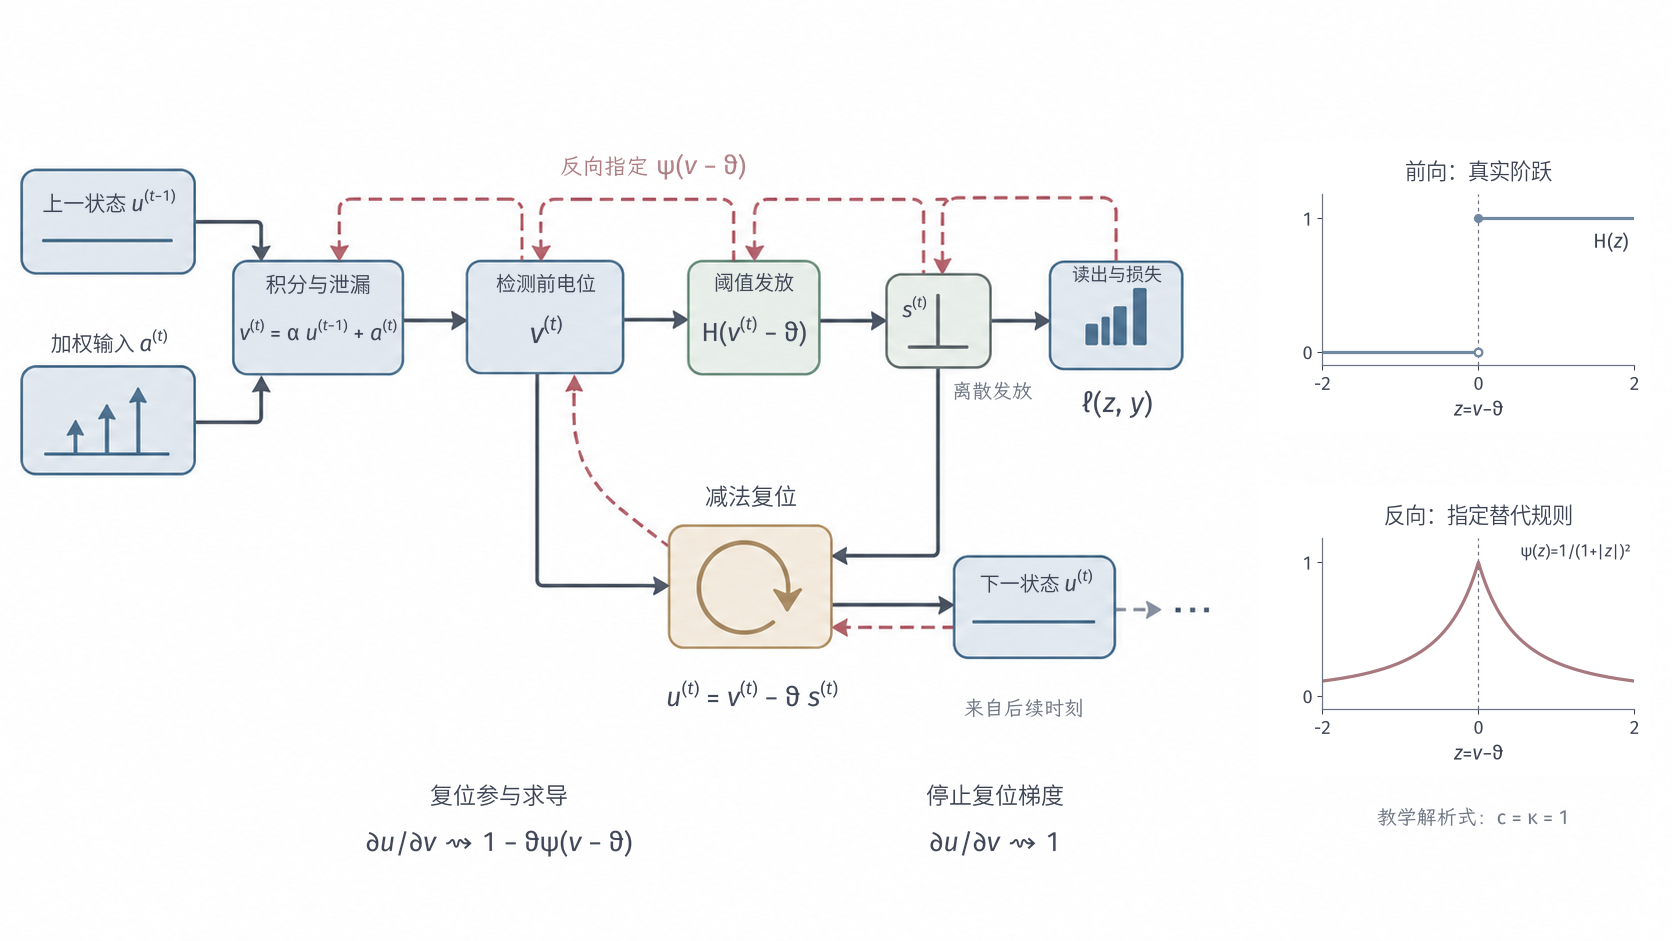
\includegraphics[width=141.563mm]{figures/03-models/02-neural-network-models/generated/snn-surrogate-forward-backward/figure.png}
  \caption{LIF前向计算与替代梯度。前向使用真实阶跃发放和减法复位；反向在发放处指定替代规则$\psi$。右侧解析曲线取$c=\kappa=1$，阶跃在零处取一；下方两式分别表示复位参与求导与停止复位梯度，两种约定不改变前向发放。}
  \label{fig:snn-surrogate-forward-backward}
\end{figure*}

将$\bm q^{(t)}$、$\bm u^{(t)}$和所需延迟状态合并为$\bm h^{(t)}$，网络可写为$\bm h^{(t)}=F_{\bm\theta}(\bm h^{(t-1)},\bm x_t)$。把这一递推展开到各个时间步，再累积所有调用同一参数的贡献，就得到第\ref{chap:recurrent-networks}章的时间反向传播；发放与复位处使用上述指定导数。在保存前向激活的实现中，较长窗口需要保存更多状态，重算可以改变这份存储代价；截断展开则删除相应历史梯度路径。所得回传信号由整套替代规则定义，其下降行为需要结合实际离散损失检验；对统一平滑目标作优化分析，还需另行建立这种规则与目标梯度的关系。

\begin{algorithm}[脉冲网络的监督训练]
  \label{alg:snn-supervised}
  \begin{algorithmic}[1]
    \Require 输入序列与标签、时间步数$K$、神经元参数、替代规则$\psi$
    \Ensure 学得的权重与读出参数
    \For{每个训练小批量}
      \State 按样本边界设置膜电位、突触状态和延迟队列
      \For{$t=1,\ldots,K$}
        \State 计算突触输入，按式\eqref{eq:snn-discrete-integrate}--\eqref{eq:snn-soft-reset}更新各层
        \State 保存反向计算所需状态并积累输出读出
      \EndFor
      \State 由读出与标签计算损失
      \State 沿展开图反向计算，以$\psi$代替发放导数并采用约定的复位导数
      \State 累积共享参数梯度，必要时裁剪，再更新参数
    \EndFor
  \end{algorithmic}
\end{algorithm}

\subsection{人工网络到脉冲网络的转换}
\label{sec:snn-conversion}

频率编码提供了另一条学习路径：先训练具有非负激活的连续值网络，再用发放率近似这些激活。\term{人工网络到脉冲网络转换}（ANN-to-SNN conversion）就是建立连续激活与脉冲统计量的对应，以复用已经学得的权重。理解这一对应，可以从不泄漏的积分发放模型开始。

设$\alpha=1$、$u^{(0)}=0$，采用减法复位，每步输入增量为$a^{(t)}$，将$K$次状态更新求和得
\begin{equation}
  \vartheta\sum_{t=1}^{K}s^{(t)}
  =\sum_{t=1}^{K}a^{(t)}-u^{(K)}\text{。}
  \label{eq:snn-conversion-balance}
\end{equation}
若输入非负且每步不超过$\vartheta$，则$0\leq u^{(K)}<\vartheta$，于是
\begin{equation}
  0\leq\frac1K\sum_{t=1}^{K}a^{(t)}
       -\frac{\vartheta}{K}\sum_{t=1}^{K}s^{(t)}
  <\frac{\vartheta}{K}\text{。}
  \label{eq:snn-conversion-error}
\end{equation}
这说明阈值乘以平均发放量可以近似平均输入，剩余电位造成有限窗口误差。比如恒定输入0.3、阈值1、窗口4步，只发放1次，对应平均值0.25，尚有0.2电位未释放。窗口10步恰好发放3次，对应0.3。该界控制已校准单元的剩余电位误差；多层网络还会接受上游发放形成的新输入。

实际转换需处理负激活、偏置、归一化和不同层的尺度。对线性层$\bm W\bm x+\bm b$，若训练后的BatchNorm使用固定均值$\mu$和方差$\sigma^2$，它的仿射变换可以折叠到权重与偏置。对输出通道$i$，有$\bm W'_{i,:}=\gamma_i\bm W_{i,:}/\sqrt{\sigma_i^2+\epsilon}$，$b'_i=\gamma_i(b_i-\mu_i)/\sqrt{\sigma_i^2+\epsilon}+\zeta_i$。这里$\gamma_i,\zeta_i$为归一化的缩放和偏移，折叠使用推理统计量。阈值或层权重再依据代表性校准数据调节，使常见激活既不会长期静默，也不会超出单步发放上限\scite{rueckauer2017conversion}

加入泄漏后，式\eqref{eq:snn-conversion-balance}会多出遗忘项；采用硬复位还会丢弃超阈值的剩余电位。多层的有限窗口误差、上游发放延迟和统计尺度偏差都可能累积。转换适合能够由非负发放统计量近似的计算。目标若使用精确相对时序，编码与动态还需保留这份时间差；端到端脉冲训练可以直接在目标窗口和读出上调整参数。

\section{理论分析}
\label{sec:snn-analysis}

\subsection{表达能力}
\label{sec:snn-temporal-stability}

脉冲网络能否区分输入，需要同时考察编码、状态和读出。若编码只给出窗口计数，原始时间顺序已经丢失，后续网络无法从计数恢复它。若编码保留时刻，有限时间常数又可能让相隔很远的事件互不影响。即使内部状态不同，最终只做总计数的读出也可能把两条轨迹合并。编码保留下来的差别经过状态和读出后是否仍可辨认，才决定整个映射的表达能力。

\subsubsection{表示精度与事件代价}
\label{sec:snn-cost}

时间离散化和编码共同决定可表示的精度。若用$K$步中的脉冲比例表示$[0,1]$内数值，读出的间隔为$1/K$；随机编码还叠加抽样方差。首次发放编码可以只用一个事件表示多个时间位置，但接收端必须等待该事件，并能区分这些位置。事件较少可以降低相应通信量，较早决策则需要在更短观察时间内获得足够证据。

设一次推理中神经元$j$发放$N_j$次，连接到$d_j$个接收突触，若每次发放都访问这些连接，则触发的突触累加数为
\begin{equation}
  C_{\mathrm{syn}}=\sum_jN_jd_j\text{。}
  \label{eq:snn-event-cost}
\end{equation}
发放次数乘上扇出，才计入事件送往多个接收端的访问。一个单元即使很少发放，大量输出连接也可能触发许多累加。按时间步模拟$m$个状态单元还需$O(Km)$次状态更新，若实现为稠密矩阵计算，未发放的连接也未必被跳过。事件驱动实现可以在到达事件时更新部分状态，但仍需处理泄漏、内部发放和延迟队列。

整次推理既有事件访问，也有状态更新、延迟队列和存储管理。任务质量与决策延迟规定输出是否可用；突触访问和状态量描述成本来源，设备测量给出整条执行链的能耗。固定输入预处理与决策条件后，才能比较稀疏活动、连接组织和硬件执行各自带来的收益。

\subsection{收敛性}
\label{sec:snn-convergence}

真实发放具有阈值切换，替代梯度规定的是近似反向信号；它未必等于离散任务目标的真实梯度。优化分析需要先固定所比较的目标与更新：可微松弛目标可在相应光滑区域和步长条件下讨论驻点，固定发放模式内的连续部分也可按其导数分析。模式切换会改变离散损失，指定回传规则是否使该损失下降则由实际训练检验；通用优化条件见第\ref{chap:neural-network-training}章。

在不跨越阈值、发放模式固定的区间，LIF状态差异会按泄漏因子衰减：相同后续输入下，单元满足$\delta u^{(t)}=\alpha\delta u^{(t-1)}$。但阈值附近的小扰动可能使某一步多发放一次，继而改变复位、突触输入和后续事件。$\alpha<1$给出这一固定模式内的泄漏衰减；整个循环网络的反馈与模式切换还会产生其他状态变化。

分析一段固定发放模式内的连续状态递推，可以像第\ref{chap:recurrent-networks}章一样检查局部Jacobian矩阵连乘。遇到阈值切换时，还需处理不连续映射、事件时刻的变化和复位。真实状态的局部Jacobian描述前向扰动，替代Jacobian描述指定的误差回传；前向稳定性分析需要使用前一种动态。较强泄漏有利于忘记过时状态，也缩短可利用的历史；循环反馈、延迟和适应状态可以改变这种取舍。

\subsection{泛化性}
\label{sec:snn-generalization}

训练和预测必须使用相容的编码、观察窗口与读出。窗口变长可能提高计数精度，却也让模型利用更多未来证据；传感器阈值、噪声与发放率变化可能改变输入分布。换设备或缩短窗口会改变实际预测条件，需要在新的输入与时间预算上重新评价所得模型。

独立试次、主体或记录可以构成抽样单位，同一连续流的相邻窗口则可能共享事件和状态。编码丢失信息影响逼近误差，有限数据与模型约束影响估计误差，替代梯度与停止时刻影响所得候选；三者应分别检查。评估划分、数据增强、正则化与集成的使用条件见第\ref{chap:neural-network-generalization}章。

\section{常见应用}
\label{sec:snn-applications}

\subsection{事件流识别}
\label{sec:snn-event-recognition}

变化驱动的视觉传感器为脉冲网络提供了直接的事件输入。\term{事件相机}（event camera）在像素亮度变化达到阈值时输出位置、时刻和变化方向，而非在固定间隔输出整帧图像。一个样本可表示为事件序列$\{(x_k,y_k,t_k,p_k)\}_{k=1}^{n_e}$，其中$(x_k,y_k)$为像素坐标，$t_k$为时间戳，$p_k\in\{-1,1\}$为亮度变化极性。这些观测记录亮度变化；恢复绝对亮度还需要初始信息或相应重建过程\scite{lichtsteiner2008sensor}

以动作片段分类为例，可以按像素和极性分输入通道，将时间戳划入宽度$\Delta t$的区间，得到输入脉冲张量。如果同一像素在一个区间多次触发，可采用事件计数，或缩短区间以保留二值表示；合并事件会改变信息。空间卷积连接提取局部变化模式，膜电位与突触状态累积时间关系，再用类别输出单元的计数或连续读出产生分数。

若类别$c$的计数为$N_c$，可以取$z_c=N_c/K$并用Softmax交叉熵训练，预测为$\argmax_c z_c$；所有计数为0时要规定平局处理或继续观察。损失可以只在片段结束计算，也可以在多个截断窗口计算以训练较早输出。在固定评价时刻比较输出，可以保持可用事件范围一致；多个窗口的监督则让模型在不同证据量下练习决策。

同一记录的相邻窗口往往共享动作、场景和事件，分散到训练与测试会让评价重复看到相关证据。按独立片段、主体或场景划分数据，才与相应新数据问题匹配；事件噪声与传感器阈值变化也要在规定的时间预算下评价。

\subsection{连续感知与动态响应}
\label{sec:snn-continuous-response}

持续感知没有天然的片段终点。网络接收不断到来的变化，保留状态，并在预定时刻或满足决策条件时产生输出。例如，一个教学运动方向检测器可用两组位置通道接收事件，再设置不同突触延迟，使某一方向依次到达的事件在下游重合；反向事件到达时没有同样的同步积累。LIF的积累与阈值把这种重合转为发放，方向读出据此给出分数。

连续输出也可以从过滤后的状态得到。设$m$维输出脉冲为$\bm s^{(t)}$，令$\bm r^{(t)}=\rho\bm r^{(t-1)}+(1-\rho)\bm s^{(t)}$，$\rho\in[0,1)$，再用$\hat{\bm y}^{(t)}=\bm C\bm r^{(t)}+\bm d$预测连续量。$\rho$越大，输出越平滑，也越迟缓；用膜电位读出则会保留阈值以下的状态。过滤参数与读出方式共同确定响应速度和抖动，任务评价据这份实际输出进行。

持续状态还会带来边界问题。静默期间应让历史影响按模型衰减；传感器重启、场景切换或长时间中断后，可以按明确规则重置状态。训练时若每个短窗口都重置，使用时却无限保留状态，网络面对的状态分布可能不同。跨窗口保留状态让早期输入继续影响预测，截断的梯度却不再把后来误差送回对应的早期计算；记忆长度与误差回传长度由此可以不同。

\section{本章小结}
\label{sec:snn-summary}

SNN把到达事件写入连续状态，以积累、泄漏、阈值和复位产生后续发放，再由读出形成预测。先后关系可以通过状态和延迟保留，计数也可以近似输入强度；编码与读出共同决定哪些差别留到输出。局部活动规则、指定的替代梯度与连续网络转换分别提供不同学习信号，训练结果据实际离散预测检验。窗口更长可降低特定编码误差，同时增加等待、事件访问和状态更新；事件稀疏性带来的收益由整条输入到设备的链路决定。

\paragraph{扩展阅读}
Gerstner等的教材从膜电位、发放与突触可塑性建立神经元动力学。其中的连续动态与本章离散更新相接，突触可塑性又为局部学习提供来源；替代梯度和转换方法则对应人工任务中的两种训练路径。观察窗口、决策延迟与设备执行把这些模型接到实际事件计算\scite{gerstner2014}

\chapter{神经网络的训练}
\label{chap:neural-network-training}

同一网络用较大步长更新时可能在谷底两侧振荡，用较小步长又可能长时间停留在高损失区。增加批量会改变梯度噪声，增加层数或序列长度还会改变误差传回早期参数的路径。反向传播给出当前位置的梯度，训练还需决定怎样使用它。目标的局部形状、估计的精度与网络的信息传播，共同决定这一步更新能产生什么进展。

各模型的求导过程已经把损失接到可训练参数上。这里将这些参数放入共同的更新过程：优化器读取梯度与历史，决定参数增量；表示尺度、连接和参数化再决定梯度怎样形成。它们可以共同使用，各自的作用沿这条计算链解释。降低训练误差需要更新找到有用的候选，这个候选在新数据上的表现则由第\ref{chap:neural-network-generalization}章分析。

设训练集为$\{(\bm x_i,y_i)\}_{i=1}^n$，所有可训练参数展平为$\bm\theta\in\mathbb R^p$，经验目标为
\begin{equation}
  \mathcal L(\bm\theta)=\frac1n\sum_{i=1}^n
  \ell(f_{\bm\theta}(\bm x_i),y_i)\text{。}
  \label{eq:training-objective}
\end{equation}
这里$p$是参数数目，$n$是样本数。第$t$次更新在$\bm\theta^{(t-1)}$处计算梯度或其估计$\bm g^{(t)}$，再得到$\bm\theta^{(t)}$。除非另行说明，公式中的平方、开方和除法作用于向量各元素；矩阵的逆和矩阵幂会明确指出。

\section{主要挑战}
\label{sec:training-challenges}

训练受阻可能来自几个环节：当前位置缺少下降信号，方向尺度相差过大，抽样梯度波动，或误差沿计算图衰减。后面的改进分别改变目标附近的更新、梯度估计与传播路径。参数大小、初始梯度及学习规则还决定可学习性分析的条件（参考\BookChapterRef{chap:deep-learning-theory}{第二卷“基础、理论和可信性”的“深度学习的可学习性”章}）。

\subsection{局部极小点与鞍点}
\label{sec:training-stationary-points}

参数梯度很小时，损失可能已经接近所求值，也可能仍有其他方向能够降低它。需要检查邻近目标怎样变化，才能决定是否继续沿当前方向、加入扰动或使用曲率。以下讨论可微目标的内部点，ReLU折点等位置则采用相应非光滑分析；驻点与目标值在非凸学习中承担不同评价作用（参考\BookSectionRef{sec:nonconvex-learning}{第二卷“基础、理论和可信性”的“一般学习的可学习性”章“非凸学习问题”节}）。

\term{驻点}（stationary point）是梯度为0的位置：一阶信息没有指出下降方向。\term{局部极小点}（local minimum）是在某个邻域内没有更低目标值的位置；若除该点外的邻近位置都更高，则是严格局部极小点。\term{全局极小点}（global minimum）要求整个参数范围内都没有更低值，因而也是局部极小点。局部邻域之外仍可能有更低目标值，因此局部极小的训练误差还需据实际数值判断。\term{局部极大点}（local maximum）则在邻域内没有更高值。可微内部极值都是驻点，但驻点还可以是极值以外的点。

在目标二阶可微的位置，\term{Hessian矩阵}（Hessian matrix）$\bm H=\nabla^2\mathcal L(\bm\theta)$描述局部曲率，即不同方向的梯度怎样随参数改变。驻点处若$\bm H$正定，该点是严格局部极小点；若负定，则是严格局部极大点。若同时有正、负特征值，就存在上升和下降方向，属于\term{鞍点}（saddle point）：从某些方向看像谷底，从另一些方向看却像山顶。正半定是二阶可微内部局部极小的必要条件；出现零方向时还需要更高阶信息。零特征值使二阶判断不充分，例如$x^4$、$-x^4$与$x^3$在0处都有零梯度、零二阶导数，却分别是极小、极大与非极值驻点。

图~\ref{fig:training-stationary-points}把“梯度为0”和“周围怎样变化”分开显示。左上图两个谷底都满足局部极小定义，右侧谷底更低；其间的峰在截面内是极大，在完整二维目标中却沿$y$方向上升，因此是鞍点。其余三个曲面强调：站在中心时梯度都为0，但离开中心后，可能处处上升、处处下降，或随方向而异。
\begin{figure*}[htbp]
  \centering
  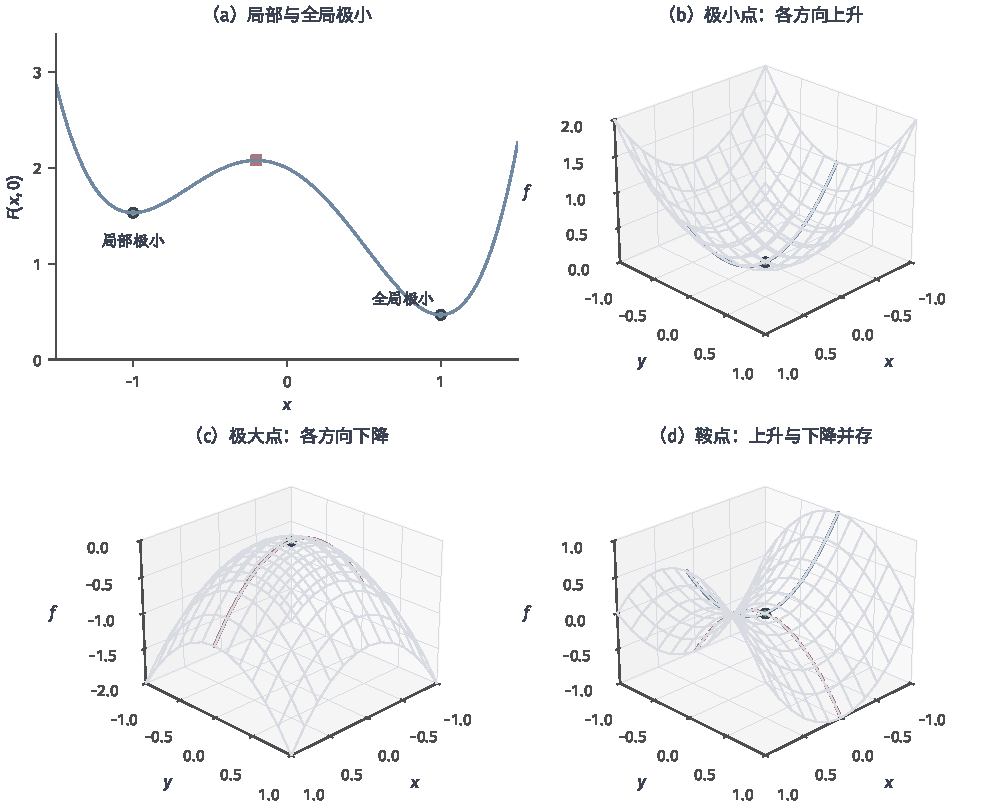
\includegraphics[width=159.059mm]{figures/03-models/02-neural-network-models/matplotlib/training-stationary-points/figure.pdf}
  \caption{驻点与极值的构造示意。（a）为$F(x,y)=1+(x^2-1)^2+0.8(x^3/3-x)+y^2$的$y=0$截面。$(-1,0)$是非全局局部极小，$(1,0)$是全局极小，方点$(-0.2,0)$是完整曲面的鞍点。（b）$f=x^2+y^2$；（c）$f=-x^2-y^2$；（d）$f=x^2-y^2$。后三图绿色中心点均为驻点，蓝色实线表示上升切片，红色线表示下降切片。图示为解析函数，不是网络损失的实测图。}
  \label{fig:training-stationary-points}
\end{figure*}

训练为何会遇到这些形状，可以从最简单的两层线性模型看起。令标量预测为$uv$、目标为1，平方损失为
\begin{equation}
  \mathcal L(u,v)=\tfrac12(uv-1)^2,\qquad
  \nabla\mathcal L=(uv-1)(v,u)^{\top}\text{。}
  \label{eq:training-factorized-saddle}
\end{equation}
损失对预测$uv$是凸的，对两层参数$(u,v)$却不是。在$(0,0)$处，梯度为0、损失为$1/2$，Hessian的两个特征值为1和$-1$。沿$u=v$的小扰动降低损失，沿$u=-v$则提高损失；只沿任一坐标轴观察，损失还保持不变。两层参数的乘积已经形成鞍点，更多参数组合、非线性与样本叠加还会改变这份几何。输出损失的凸性因而需要和参数空间的性质分别判断。

\term{平坦区域}（flat region）指在所考察尺度内目标或梯度变化很小的区域，不必包含严格驻点。饱和激活、参数冗余或近似对称性都可能产生这类区域。在这种区域内，损失值说明离训练目标多远，梯度尺度和邻近更新则说明当前位置能提供多少推进信号。

梯度下降若精确到达零梯度驻点，就没有一阶更新；在其附近，梯度很小也会让推进缓慢。鞍点还有可下降方向，但小梯度未必明显指向它；非全局局部极小则需要离开当前邻域才能到达更低区域。高维鞍点及附近平台的研究将小梯度与可下降方向联系起来，为判断停滞提供了曲率依据\scite{dauphin2014saddle}

扰动在可下降方向上有分量时，可能将参数送离某些鞍点或平台；若每个样本在零参数处的梯度都为0，抽样也会继续给出0。参数置换和尺度对称还让同一个预测函数对应多个参数位置。驻点性质描述当前位置的目标形状，训练误差描述样本拟合，泛化风险则描述新数据预测。

\subsection{病态曲率}
\label{sec:training-curvature}

一个方向陡、另一个方向缓时，同一学习率需要同时照顾两种变化速度。即使目标只有一个全局极小点，也可能出现这种更新困难；分解参数化还会改变相应动力学（参考\BookEquationRef{eq:factorized-gradient-flow}{第二卷“基础、理论和可信性”的“深度学习的可学习性”章中的分解参数梯度流公式}）。考虑教学目标
\begin{equation}
  q(\bm\theta)=\tfrac12(a\theta_1^2+b\theta_2^2),
  \qquad a\gg b>0\text{。}
  \label{eq:training-quadratic}
\end{equation}
两个方向分别以$a$和$b$的尺度变化。固定步长梯度下降在第一个方向的系数为$1-\eta a$，在第二个方向为$1-\eta b$。要让任意初始位置的两个方向都收缩，必须取$0<\eta<2/a$；这个步长在缓方向却只能带来很小的变化。

\term{病态曲率}（ill-conditioned curvature）描述不同方向的曲率尺度相差很大的情形。正定二次目标的\term{条件数}（condition number）为$\kappa=\lambda_{\max}(\bm H)/\lambda_{\min}(\bm H)$。在该模型中，最优固定步长$2/(a+b)$对应的最坏方向收缩因子为$(\kappa-1)/(\kappa+1)$，条件数大时接近1。若步长让陡方向的系数为负，参数会交替越过谷底，表现为振荡。

取$a=100,b=1,\eta=0.015$，陡方向每步乘以$-0.5$，缓方向每步乘以0.985。图~\ref{fig:training-curvature}左图显示这个稳定步长下的轨迹：左右振荡迅速缩小，轨迹落到谷底附近，但第80步仍未到达极小点。此时是收敛慢，继续迭代仍会趋向原点。

为了加快缓方向，若把步长增到临界值$\eta=2/a=0.02$，陡方向系数就变为$-1$。右图从上方观察同一谷地：$\theta_1^{(t)}=0.35(-1)^t$一直在两侧来回切换，$\theta_2^{(t)}=0.98^t$虽然逐渐减小，却不能带动陡方向的摆幅收缩。损失趋向$100\times0.35^2/2=6.125$，而最小值是0；这时增加迭代次数也无法收敛到原点。步长再大还会发散。两图共同显示了单一全局步长的矛盾：照顾陡方向时缓方向走得慢，试图加快缓方向又可能在陡方向越过头。动量利用历史方向缓解某些振荡，\term{预条件}（preconditioning）则通过矩阵或逐坐标尺度变换，让更新适应不同方向的变化速度。
\begin{figure*}[htbp]
  \centering
  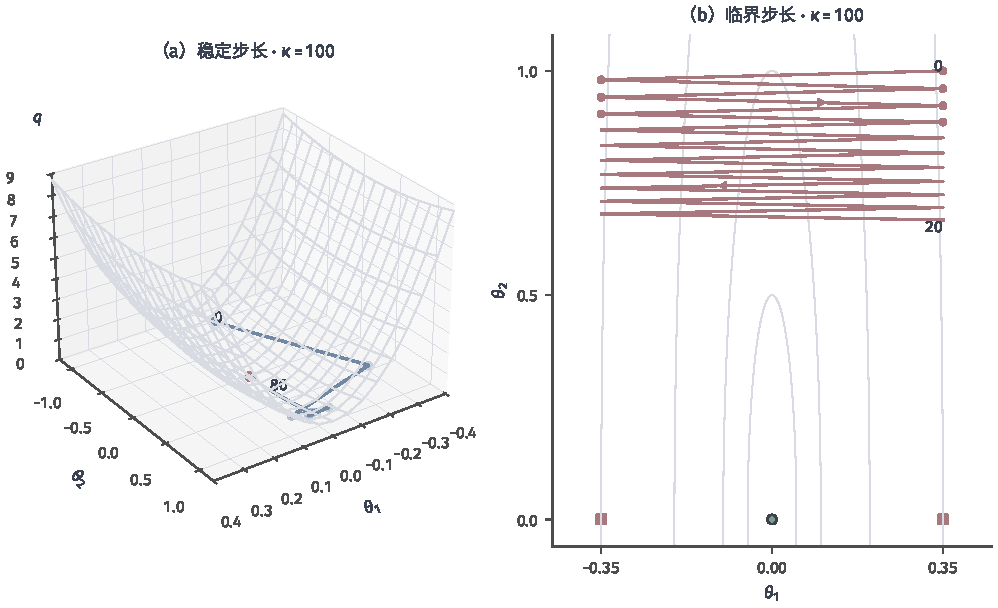
\includegraphics[width=159.059mm]{figures/03-models/02-neural-network-models/matplotlib/training-curvature/figure.pdf}
  \caption{同一病态二次目标在两种步长下的轨迹，标题直接标出条件数$\kappa=a/b=100$，绿色点为极小点。（a）三维图采用稳定步长0.015，蓝色实心圆标出第0--8步，空心圆标出第80步；陡方向收缩快，谷底推进慢。（b）俯视投影采用临界步长0.02，深红线连接第0--20步，实心圆标出第0--6步，空心圆为第20步；灰线为等高线，竖虚线为谷底。左右摆幅保持0.35，损失趋向6.125而无法达到原点处的0。}
  \label{fig:training-curvature}
\end{figure*}
\FloatBarrier

重缩放同一函数的参数坐标，会改变Hessian特征值与梯度下降轨迹，归一化和重参数化因此也会影响优化。上面的条件数与收缩率针对正定二次目标；非凸区域还要处理零或负曲率。

\subsection{非精确梯度}
\label{sec:training-inexact-gradients}

完整经验梯度需要访问全部样本。小批量用抽到的样本估计这份梯度，估计的波动和系统偏差会以不同方式进入更新；随机梯度的结论也以抽样、步长和损失为条件（参考\BookSectionRef{sec:sgd-stability}{第二卷“基础、理论和可信性”的“一般学习的可学习性”章“凸学习问题的随机梯度下降”小节}）。每步选$b$个样本组成索引集合$B^{(t)}$，计算
\begin{equation}
  \bm g^{(t)}=\frac1b\sum_{i\in B^{(t)}}
    \nabla_{\bm\theta}\ell(f_{\bm\theta^{(t-1)}}(\bm x_i),y_i)\text{。}
  \label{eq:training-minibatch-gradient}
\end{equation}
若在给定当前参数后独立、均匀、有放回抽样，条件期望等于完整经验梯度。独立抽样下，其协方差为单样本梯度协方差的$1/b$；无放回抽样还有有限总体修正。按顺序遍历一段相关视频，或在一个轮次内随机重排后逐批读取，并不满足这一条件独立模型。

\term{随机方差}（stochastic variance）描述梯度估计围绕期望的波动，\term{系统性偏差}（systematic bias）则是估计期望与目标梯度的差异。扩大独立批量降低抽样方差；截断时间反向传播删除历史路径、错误缩放改变目标贡献，则需要修正相应计算。量化、有限精度和近似算子还会引入数值误差，是否具有偏差取决于具体实现。

梯度累积可以把多个小批量的梯度合成为较大批量更新，但要求它们在同一参数位置计算，并按样本数或有效词元数正确加权。BatchNorm等依赖当前批量的操作、随机失活及不同长度掩码，会使“分批累积”与“一次大批量前向”具有不同计算图。批量还决定每轮包含多少次更新，因此更新步数、样本访问量与时间预算构成三种不同的比较条件。

\subsection{梯度传播与长期依赖}
\label{sec:training-gradient-propagation}

误差从输出传到早期表示，需要穿过沿途的局部导数。即使输出梯度与抽样估计准确，连乘仍可能使某些方向的信号衰减或放大。残差、门控、初始化与参数约束通过改变这些路径或因子参与训练。对于$L$层复合映射，记$\bm J_l=\partial\bm h^{(l)}/\partial\bm h^{(l-1)}$，若梯度按列向量表示，则
\begin{equation}
  \nabla_{\bm h^{(s)}}\ell
  =\bm J_{s+1}^{\top}\cdots\bm J_L^{\top}
    \nabla_{\bm h^{(L)}}\ell\text{。}
  \label{eq:training-jacobian-chain}
\end{equation}
沿某些方向反复缩小，会形成\term{梯度消失}（vanishing gradients）；反复放大，则可能形成\term{梯度爆炸}（exploding gradients）。算子范数给出上界$\lVert\nabla_{\bm h^{(s)}}\ell\rVert_2\leq\prod_{l>s}\lVert\bm J_l\rVert_2\,\lVert\nabla_{\bm h^{(L)}}\ell\rVert_2$。上界描述可能的最大放大；实际梯度沿哪些方向传播，还取决于奇异向量对齐和各支路的抵消。

循环网络沿时间重复使用状态映射，出现同类Jacobian矩阵连乘。饱和激活的小导数、权重尺度、网络深度和递推长度都会影响传播。裁剪处理已经算出的异常大值，接近0的历史信号则需要改变传播路径。前向状态怎样保存输入、后来的损失怎样影响早期参数，是同一计算图上的两个问题。

\section{优化方法}
\label{sec:training-optimizers}

一次参数更新需要决定往哪里走、走多远，以及当前梯度有多少可以信任。第\ref{sec:training-challenges}节的目标几何、病态曲率和非精确梯度，分别给这三个决定带来困难。方向、尺度与噪声分别对应不同的更新机制：
\begin{itemize}
  \item \textbf{下降方向。} 负的完整梯度给出欧氏坐标下的局部最陡下降方向，但弯曲谷地中沿这个方向反复更新可能绕路；小批量梯度还会偏离完整目标的方向。动量借助历史判断持续趋势，预条件和曲率方法利用方向间的耦合修正更新。小梯度区域的曲率与损失值再决定当前信号是否已经接近所求目标。
  \item \textbf{下降尺度。} 步长过小会让训练长时间停留在高损失区，过大又可能跨过谷底、持续振荡甚至发散。希望方法同时管理整体学习率和不同方向的相对尺度，在缓方向充分推进，在陡方向限制更新，并随训练阶段减小需要精细调整时的步幅。调度、逐坐标缩放、阻尼和步长搜索分别处理这些尺度选择。
  \item \textbf{噪声适应。} 小批量梯度会随样本改变，异常大值、稀疏访问和非平稳统计又会使历史参照失准。批量平均、历史平滑、遗忘机制与裁剪可以控制其中不同部分；过强平滑会滞后，过大步长会放大噪声，过快遗忘则难以识别趋势。截断计算和错误缩放产生的偏差则需要处理其来源。
\end{itemize}
方向与尺度需要一起判断。精确下降方向也可能因步长过大而提高损失，较小更新则可能只是停滞。更复杂的估计还会增加求解、通信和历史状态，达到同一训练目标的总时间与峰值存储将这些额外开销计入比较。非凸目标上的这些改进依赖相应条件；计算图内部已经消失的梯度，仍需在第\ref{sec:training-connections}节改善传播路径，泛化表现则由第\ref{chap:neural-network-generalization}章另行判断。

为了比较不同方法，可以把优化器看成一个带记忆的更新过程：接收当前位置的信息，读取历史状态，按规则计算参数增量，再保存下一步需要的状态。沿这个更新过程，可以检查四种信息：
\begin{itemize}
  \item \textbf{输入。} 基本方法接收当前参数与完整或抽样梯度；曲率方法还使用Hessian、输出Jacobian矩阵或Fisher相关信息，步长搜索还需评估候选位置的损失。输入的精度、抽样方式和获取成本，限定了方法能作出怎样的判断。
  \item \textbf{状态。} 无动量SGD不保存与参数同规模的历史缓冲；动量保存方向，AdaGrad与RMSProp保存平方梯度统计，Adam同时保存两种矩，L-BFGS保存有限组参数差与梯度差。状态还可能是分层矩阵、行列因子和调度进度，其大小与遗忘方式决定成本和适应速度。
  \item \textbf{方法。} 可直接沿梯度缩放，也可先平滑方向、按坐标调整尺度、求解耦合方向的线性系统，或提取符号、整形奇异值。裁剪、阻尼、偏差修正与学习率调度可以参与这个计算；近似方式决定保留哪些关系、舍弃哪些信息。
  \item \textbf{输出。} 对训练循环而言，输出是参数增量$\Delta\bm\theta^{(t)}$或等价的新参数，以及更新后的历史状态。增量的方向、长度、坐标比例和可行性显示前三项怎样进入实际更新；预条件和历史状态还会改变原始梯度上限对应的位移。
\end{itemize}

这四个维度描述同一个优化器，可以交叉组合。例如，SGD以当前梯度为输入、没有方向历史，方法是乘以学习率，输出$\Delta\bm\theta^{(t)}=-\eta_t\bm g^{(t)}$；Adam仍以当前梯度为主要输入，却用两种历史状态构造平滑方向与逐坐标尺度，因此输出的方向和长度都可能不同。共同的梯度输入经过不同状态与计算，产生不同增量；平方梯度统计记录历史幅度，Hessian记录当前位置的曲率。

下面沿这个共同过程展开：基本更新、调度和裁剪建立基准；动量与自适应方法增加历史状态；牛顿、拟牛顿、GGN和自然梯度使用更强的几何信息或估计；K-FAC、Shampoo和Muon利用层或矩阵结构改变计算与输出。这些方法各自保留不同几何信息，其实际增量和成本由具体输入、状态及计算规则确定。

在共同记号下，可将许多更新写为$\bm\theta^{(t)}=\bm\theta^{(t-1)}-\eta_t\bm P^{(t)}\bm d^{(t)}$。$\bm d^{(t)}$由当前梯度及历史信息构成，$\bm P^{(t)}$为尺度变换或预条件矩阵，$\eta_t$为全局学习率。这个分解帮助辨认方法改变了方向、逐坐标尺度，还是随训练进程变化的整体步长；有些实现直接求方向或计算矩阵作用，无需显式保存$\bm P^{(t)}$。

\subsection{梯度下降与随机梯度下降}
\label{sec:training-gradient-schedules}

基本更新将当前完整梯度或抽样梯度按步长缩放，再从参数中减去（参考\BookSectionRef{sec:opt-gradient-descent}{第一卷“数学准备”的梯度下降小节}和\BookSectionRef{sec:opt-stochastic-gradient-stability}{第一卷“数学准备”的近似更新方法小节}）。对网络训练目标$\mathcal L$使用完整梯度或小批量梯度$\bm g^{(t)}$，更新为
\begin{equation}
  \bm\theta^{(t)}=\bm\theta^{(t-1)}-\eta_t\bm g^{(t)}\text{。}
  \label{eq:training-sgd}
\end{equation}
在更新线段内目标梯度为$L_s$-Lipschitz时，下降引理给出完整梯度在$0<\eta<2/L_s$下的下降界；梯度非零时严格下降，驻点处保持不动。ReLU切换点改变光滑条件，抽样噪声改变所用方向；相应更新按各自条件分析。

小批量SGD的每一步既受到当前下降方向影响，也受到抽样噪声影响。
在本步所有可能的更新线段上满足同一光滑条件时，若$\bm g=\nabla\mathcal L+\bm\xi$，给定当前参数时
$\mathbb E[\bm\xi\mid\bm\theta]=\bm0$且$\mathbb E[\lVert\bm\xi\rVert_2^2\mid\bm\theta]<\infty$，
代入光滑性上界并取条件期望，得到
\begin{equation}
  \begin{aligned}
  \mathbb E[\mathcal L(\bm\theta-\eta\bm g)\mid\bm\theta]
  \leq{}&\mathcal L(\bm\theta)
    -\eta(1-L_s\eta/2)\lVert\nabla\mathcal L\rVert_2^2\\
    &+\tfrac12L_s\eta^2\mathbb E[\lVert\bm\xi\rVert_2^2\mid\bm\theta]\text{。}
  \end{aligned}
  \label{eq:training-stochastic-descent}
\end{equation}
噪声项随$\eta^2$增长；当真实梯度很小时，它可能抵消这一步的预期下降。减小步长或扩大独立批量可以改变这项，但也改变推进速度和计算量。在梯度较小的后期，这份波动就可能成为更新的主要成分。

SGD的优势是更新简单、额外状态少，小批量避免每一步遍历全部数据；完整梯度则消除了抽样方差，更便于判断局部下降。代价分别是随机波动和较高的数据访问成本，而且两者都用同一全局步长面对不同方向的曲率。一次基本更新不额外维护与$p$同规模的历史状态。前向、反向和数据访问共同决定每步时间，与所需步数一起构成完整训练成本。

\subsection{学习率调度}
\label{sec:training-schedules}

式\eqref{eq:training-stochastic-descent}中，推进项随步长增长，噪声项却随步长平方增长；训练早期与接近解时未必需要相同尺度。调度通过改变整体步长处理这一阶段差异。\term{学习率调度}（learning rate scheduling）按训练进程改变$\eta_t$。固定学习率维持同一更新尺度；分段衰减在预定里程碑乘以小于1的系数；指数衰减可以写为$\eta_t=\eta_0\gamma^t$，$0<\gamma<1$。若固定总训练长度，余弦调度可将学习率从$\eta_{\max}$平滑降到$\eta_{\min}$：
\begin{equation}
  \eta_t=\eta_{\min}+\frac{\eta_{\max}-\eta_{\min}}2
  \left[1+\cos\left(\frac{\pi(t-t_w)}{T-t_w}\right)\right],
  \quad t_w\leq t\leq T\text{。}
  \label{eq:training-cosine-schedule}
\end{equation}
这里$T$为总更新次数，$t_w$为预热结束步，总步数须大于预热步数。\term{预热}（warmup）在训练早期逐步增加学习率，有预热时，例如前$t_w$步取$\eta_t=\eta_{\max}t/t_w$，让初始参数和优化器统计量在较小更新下开始适应。周期性调度则反复升降，带重启的余弦调度是其中一种形式\scite{loshchilov2017sgdr}

调度以很小的额外成本区分早期推进与后期精细调整，预热还能限制尚未稳定的初始更新。但衰减过早可能在高损失区停滞，过晚可能延长解附近的波动；预定总长度也未必适应中途改变的预算。调度可以按更新步、样本访问量或训练轮次计时，这些单位在批量改变时不再等价。全局$\eta_t$决定整步的基础尺度，后面的自适应方法再调整相对尺度。预热与衰减只改变整步尺度，所用梯度和候选目标仍需满足相应训练条件。

例如，计划训练1000步，前100步线性预热，随后用式\eqref{eq:training-cosine-schedule}衰减。第100步恰好到达$\eta_{\max}$，第550步为两端学习率的平均，第1000步到达$\eta_{\min}$。若恢复第550步的参数却从调度起点重新计时，后续轨迹就与原计划不同。调度状态因此属于恢复训练所需的信息。

\subsection{梯度裁剪}
\label{sec:training-gradient-modification}

第\ref{sec:training-gradient-propagation}节中的连乘可能产生偶发的大梯度，数值误差也可能放大更新，使参数离开当前有用区域。\term{梯度裁剪}（gradient clipping，也称梯度截断）在优化器使用梯度之前限制这份信号。逐元素裁剪令$\tilde g_j=\max(-c,\min(c,g_j))$，$c>0$，它改变部分坐标的相对比例；整体范数裁剪则为
\begin{equation}
  \tilde{\bm g}=\bm g\min\left(1,\frac{c}{\lVert\bm g\rVert_2}\right)\text{，}
  \label{eq:training-norm-clipping}
\end{equation}
零梯度直接保留。整体裁剪在非零时保持方向，但会引入与梯度大小有关的偏差。裁剪后的梯度还可能被动量或自适应尺度放大，所以梯度范数上限不等于最终参数步长上限。

取$\bm g=(3,4)^{\top}$，范数为5，整体上限$c=2$给出$(1.2,1.6)^{\top}$；逐元素上限2则给出$(2,2)^{\top}$，方向已改变。两种裁剪都控制极端更新，小于上限的信号保持原样。若几乎每步都被大幅裁剪，损失缩放、初始化或状态递推可能持续产生过大梯度，需要定位这份来源。

\subsection{动量法}
\label{sec:training-momentum}

陡方向的梯度可能来回变号，缓方向却持续指向谷底。把历史与当前方向累积起来，同向部分得到保留，交替部分可以抵消（参考\BookSectionRef{sec:opt-curvature-acceleration}{第一卷“数学准备”的动量与加速小节}）。采用未归一化的累积约定，从零缓冲开始，令
\begin{equation}
  \bm m^{(t)}=\beta\bm m^{(t-1)}+\bm g^{(t)},\qquad
  \bm\theta^{(t)}=\bm\theta^{(t-1)}-\eta_t\bm m^{(t)},
  \quad\beta\in[0,1)\text{。}
  \label{eq:training-momentum}
\end{equation}
交替的梯度会部分抵消，持续同向的梯度会积累。如果$\bm g^{(t)}$近似恒定，累积量趋向$\bm g/(1-\beta)$，因此调整$\beta$也改变有效更新尺度。另一约定在梯度前乘$1-\beta$；比较实现时要同时对应学习率。

精确二次目标中的误差递推可以给出谱速率，网络训练中的曲率和抽样梯度则随位置变化。较大的$\beta$延长历史记忆，同时放大未归一化缓冲的有效尺度；系数选择据实际目标与更新评价。

动量只增加一个$p$维缓冲，但也使更新具有惯性。梯度突然换方向时，旧方向不会立即消失；较大的$\beta$提供更长历史，也可能让响应迟缓。它对噪声的平滑和对有效步长的放大应一起考虑。

\subsection{Nesterov加速梯度}
\label{sec:training-nesterov}

动量保存旧方向，也可能在接近谷底时继续推动参数。Nesterov方法让梯度读取历史方向预计到达的位置，以修正这种惯性。\term{Nesterov加速梯度}（Nesterov accelerated gradient, NAG）在历史方向指向的前瞻位置计算梯度，而不是只对当前位置的梯度做累积。对式\eqref{eq:training-momentum}的约定，可写为
\begin{align}
  \bar{\bm\theta}^{(t)}&=\bm\theta^{(t-1)}-\eta_t\beta\bm m^{(t-1)},\\
  \bm m^{(t)}&=\beta\bm m^{(t-1)}+
       \nabla\mathcal L(\bar{\bm\theta}^{(t)}),\qquad
  \bm\theta^{(t)}=\bm\theta^{(t-1)}-\eta_t\bm m^{(t)}\text{。}
  \label{eq:training-nesterov}
\end{align}
前瞻梯度提供对惯性方向的修正。深度学习实现常采用等价变换或固定动量的变体；经典加速率分析以凸目标和相应系数为条件，非凸抽样更新还需另外分析。

以一维$q(\theta)=a\theta^2/2$为例，普通动量读取$a\theta$，前瞻形式读取$a(\theta-\eta\beta m)$。若惯性正将参数推向谷底，前瞻梯度已看到较低位置，从而减少继续沿旧方向推进的量；若已越过谷底，则可能更早得到相反方向的修正。这组一维计算展示前瞻怎样修正方向，实际下降还取决于曲率与步长。

式\eqref{eq:training-nesterov}直接展示“到前瞻位置求导”的定义。实际实现也可把参数位置作等价重写，以避免额外前向计算；变动学习率或动量时，等价关系需要重新对应。求导位置、缓冲约定和最终增量共同确定不同实现是否对应同一更新。

前瞻的优势是让惯性修正在本步方向形成前发生，在相应凸条件下可得到加速结论。它仍保留动量的历史滞后，也会受到前瞻位置梯度噪声的影响；非凸网络中前瞻点可能落入与当前位置不同的局部形状。前瞻因此改变方向的形成方式，步长与动量继续决定该方向产生的位移。

\subsection{AdaGrad}
\label{sec:training-adaptive}

有些参数经常收到大梯度，有些只在少数样本出现时更新，同一全局步长无法分别照顾两者。\term{自适应学习率}（adaptive learning rate）用历史梯度统计量为不同坐标设置相对尺度。逐坐标统计比完整矩阵便宜，但不完整描述第\ref{sec:training-curvature}节中的方向耦合；历史统计记录观测梯度的大小与频率，局部曲率则还包含方向之间的耦合。

AdaGrad累计逐坐标平方梯度。令$\bm v^{(0)}=\bm0$，其常见对角形式为
\begin{equation}
  \bm v^{(t)}=\bm v^{(t-1)}+\bm g^{(t)}\odot\bm g^{(t)},\qquad
  \bm\theta^{(t)}=\bm\theta^{(t-1)}-
  \eta\frac{\bm g^{(t)}}{\sqrt{\bm v^{(t)}}+\epsilon}\text{。}
  \label{eq:training-adagrad}
\end{equation}
$\odot$为逐元素乘法，$\epsilon>0$防止分母为0。反复收到大梯度的坐标逐渐减小更新尺度，较少更新的坐标则保留较大相对尺度。累积量不减小，长期训练中步长可能变得过小\scite{duchi2011adagrad}

若某个坐标每步收到相同的非零梯度$g$，忽略$\epsilon$时，第$t$步的更新幅度为$\eta/\sqrt t$；梯度的绝对尺度被平方累积抵消。一个很少出现的特征则只在出现时增加该坐标累积量，因此按访问次数减小步长。按访问次数累积的尺度使稀疏坐标获得不同步幅；其训练效果还与目标、数据和所选学习率有关。

AdaGrad增加一个$p$维累积量，每步的逐元素处理为$O(p)$。累计统计无法主动忘记训练早期的大梯度：目标分布或训练阶段改变后，早期尺度仍会限制当前更新。RMSProp接下来用有限记忆缓解这一点。

\subsection{RMSProp}
\label{sec:training-rmsprop}

AdaGrad的累计历史不遗忘，早期大梯度可能长期压低后续步长。若训练阶段的尺度改变，指数平均可以让近期梯度重新决定分母。RMSProp改用近期平方梯度的指数移动平均：$\bm v^{(t)}=\rho\bm v^{(t-1)}+(1-\rho)\bm g^{(t)}\odot\bm g^{(t)}$，再用式\eqref{eq:training-adagrad}中的分母更新，$\rho\in[0,1)$。旧梯度影响衰减，因此相对尺度可以随着训练阶段改变。其平方平均、开方和稳定项的位置应以具体实现为准\scite{hinton2012rmsprop}

为明确它与AdaGrad的不同，把更新完整写为
\begin{equation}
  \begin{aligned}
  \bm v^{(t)}&=\rho\bm v^{(t-1)}+(1-\rho)\bm g^{(t)}\odot\bm g^{(t)},\\
  \bm\theta^{(t)}&=\bm\theta^{(t-1)}-
    \eta_t\bm g^{(t)}/(\sqrt{\bm v^{(t)}}+\epsilon)\text{。}
  \end{aligned}
  \label{eq:training-rmsprop}
\end{equation}
过去第$s$步平方梯度在第$t$步的权重为$(1-\rho)\rho^{t-s}$。较大的$\rho$使尺度变化更平缓，却更慢适应新梯度；较小的$\rho$响应更快，也增加分母波动。零初值下的恒定梯度给出$v^{(t)}=(1-\rho^t)g^2$，因此早期分母尚未达到稳态，初始更新可能比稳态更大。

基本RMSProp使用一个$p$维二阶矩状态，可另外组合动量。它观察的是当前坐标的历史平方梯度，对坐标旋转通常不具有不变性，也不利用坐标之间的耦合。全局学习率仍控制整体步幅，坐标间尚未记录的耦合则可能继续影响曲率适配。

\subsection{AdaDelta}
\label{sec:training-adadelta}

只根据平方梯度设置分母，仍需选择参数实际移动的尺度。AdaDelta把近期更新也纳入统计，用更新与梯度的两类均方根之比调节幅度，减少对单一固定全局尺度的依赖。设$\bm v^{(t)}$为上述平方梯度平均，$\bm r^{(t)}$为平方更新平均，则原始基本形式为
\begin{align}
  \Delta\bm\theta^{(t)}&=-\frac{\sqrt{\bm r^{(t-1)}+\epsilon}}
                               {\sqrt{\bm v^{(t)}+\epsilon}}
                                \odot\bm g^{(t)},\\
  \bm r^{(t)}&=\rho\bm r^{(t-1)}+(1-\rho)
      \Delta\bm\theta^{(t)}\odot\Delta\bm\theta^{(t)},\\
  \bm\theta^{(t)}&=\bm\theta^{(t-1)}+\Delta\bm\theta^{(t)}\text{。}
  \label{eq:training-adadelta}
\end{align}
分子使用前一步统计量，避免与本步更新形成循环定义。这个基本形式没有独立的全局学习率，但仍需选择$\rho$、稳定项和初值；有些实现再乘全局系数，相应尺度也进入实际增量\scite{zeiler2012adadelta}

如果某个坐标近期更新很小，分子会减小该坐标的更新；梯度尺度上升时，分母则抑制幅度。分子与分母共同把近期参数变化和近期梯度联系起来，这是它区别于仅累计梯度平方的方法之处。两个状态均按坐标保存，额外存储为$O(p)$，但常数是两组统计量。

稳定项同时承担零初值启动的作用。如果$r^{(0)}=0$且完全去掉$\epsilon$，第一步分子就为0；尚未发生的更新因而没有为分子提供初始尺度。实际$\epsilon$的数值与单位、$\rho$及全局缩放约定都会影响轨迹。

\subsection{Adam与AMSGrad}
\label{sec:training-adam}

抽样噪声影响方向，坐标尺度差异影响幅度；单独的动量或平方统计各处理一部分。Adam同时维护梯度的一阶矩和非中心化二阶矩，前者给平滑方向，后者给逐坐标尺度，以较低的逐元素计算成本组合两种处理。AMSGrad进一步管理分母随时间变化的问题。以零初值定义
\begin{align}
  \bm m^{(t)}&=\beta_1\bm m^{(t-1)}+(1-\beta_1)\bm g^{(t)},\\
  \bm v^{(t)}&=\beta_2\bm v^{(t-1)}+(1-\beta_2)
                 \bm g^{(t)}\odot\bm g^{(t)},\\
  \hat{\bm m}^{(t)}&=\frac{\bm m^{(t)}}{1-\beta_1^t},\qquad
  \hat{\bm v}^{(t)}=\frac{\bm v^{(t)}}{1-\beta_2^t},\\
  \bm\theta^{(t)}&=\bm\theta^{(t-1)}-
    \eta_t\frac{\hat{\bm m}^{(t)}}{\sqrt{\hat{\bm v}^{(t)}}+\epsilon}\text{。}
  \label{eq:training-adam}
\end{align}
$\beta_1,\beta_2\in[0,1)$为平滑系数。分母中的修正因子来自零初值：把$\bm m^{(0)}=\bm0$代入递推，假设第1至$t$步梯度具有相同的有限均值$\mathbb E[\bm g^{(s)}]=\bm\mu$，就有
\begin{equation}
  \begin{aligned}
    \bm m^{(t)}&=(1-\beta_1)\sum_{s=1}^{t}\beta_1^{t-s}\bm g^{(s)},\\
    \mathbb E[\bm m^{(t)}]
      &=(1-\beta_1)\sum_{s=1}^{t}\beta_1^{t-s}\bm\mu
        =(1-\beta_1^t)\bm\mu\text{。}
  \end{aligned}
  \label{eq:training-adam-bias-correction}
\end{equation}
第二行只用期望的线性性质与等比求和，不要求各步梯度相互独立。有限步的权重和是$1-\beta_1^t$，尚未达到1；除以它，便在上述同均值假设下得到$\mathbb E[\hat{\bm m}^{(t)}]=\bm\mu$。同理，若各步的逐坐标非中心二阶矩均为$\bm\nu=\mathbb E[\bm g^{(s)}\odot\bm g^{(s)}]$且有限，零初值$\bm v^{(0)}=\bm0$给出$\mathbb E[\bm v^{(t)}]=(1-\beta_2^t)\bm\nu$。这里没有减去梯度均值，$\bm\nu$不是梯度方差。偏差修正消除的是零初始化的权重缺口；实际梯度统计随参数变化，抽样偏差由取样方式决定，当前矩与历史平均的差别则随参数变化保留\scite{kingma2015adam}

这里的二阶矩是$g_j^2$的平均，Hessian是损失对参数的二阶导数。前者即使在负曲率区域也非负，且包含梯度均值和噪声方差；后者可以有负特征值。Adam属于用一阶梯度统计构造更新的方法。全局学习率和调度继续决定整步位移，训练速度与泛化风险再在共同任务和预算下比较。

Adam的第一次更新很有辨识度：零初值下，偏差修正后$\hat m^{(1)}=g^{(1)}$、$\hat v^{(1)}=(g^{(1)})^2$，所以忽略$\epsilon$时，非零坐标按$-\eta_1\operatorname{sign}(g^{(1)})$移动。后续步由不断改变的历史方向和尺度共同决定，更新比例随之变化。两组$p$维状态增加存储，恢复训练时也必须恢复它们。

Adam的指数平均可能降低分母，使某个坐标的有效步长重新增大。\term{AMSGrad}用历史最大二阶矩阻止这种下降。省略初始化偏差修正时，可写为
\begin{equation}
  \bar{\bm v}^{(t)}=\max(\bar{\bm v}^{(t-1)},\bm v^{(t)}),\qquad
  \bm\theta^{(t)}=\bm\theta^{(t-1)}-
    \eta_t\bm m^{(t)}/(\sqrt{\bar{\bm v}^{(t)}}+\epsilon)\text{，}
  \label{eq:training-amsgrad}
\end{equation}
最大值逐元素计算，$\bar{\bm v}^{(0)}=\bm0$。加入偏差修正的实现还需对应其具体约定。AMSGrad针对Adam的某些收敛问题提出，但其收敛分析针对相应目标与更新条件；历史最大值限制后期分母下降，同时减少对较小梯度尺度的适应\scite{reddi2018amsgrad}

图~\ref{fig:training-optimizer-trajectories}把SGD、动量和Adam放到同一个病态二次目标上逐步计算。SGD在陡方向反复越过谷底，缓方向只按固定比例缩小；动量利用历史方向加快沿谷底推进，但仍带有惯性振荡；Adam在这个轴对齐例子中按坐标缩放，前几步几乎沿对角线接近原点。三条轨迹对应图中各自给定的超参数，显示同一目标中方向与尺度怎样进入更新。
\begin{figure}[htbp]
  \centering
  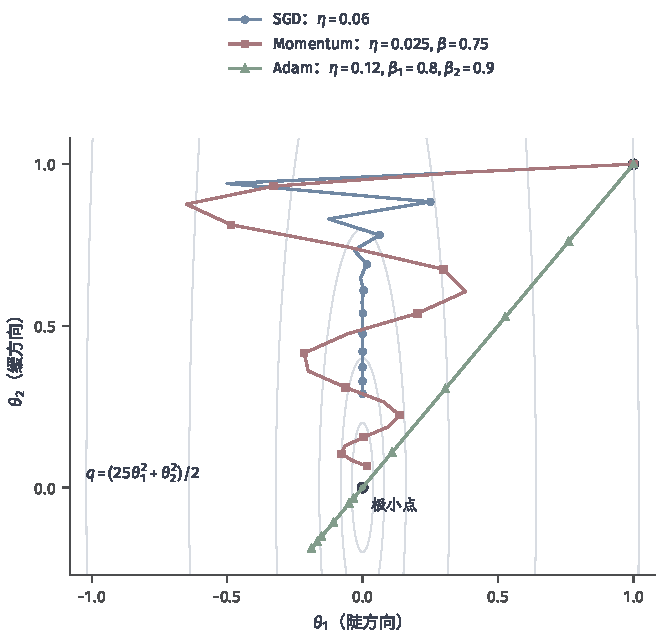
\includegraphics[width=105.412mm]{figures/03-models/02-neural-network-models/matplotlib/training-optimizer-trajectories/figure.pdf}
  \caption{SGD、动量与Adam在同一病态二次目标上的前20步。目标为$q(\bm\theta)=(25\theta_1^2+\theta_2^2)/2$，条件数$\kappa=25$，三者均从$(1,1)^\top$出发并使用完整梯度；灰线为等高线，绿色点为唯一极小点。轨迹由正文定义的递推式直接计算，图例列出步长和矩系数。图示比较固定了目标与起点，超参数改变后速度与振荡也会改变；一般非凸抽样训练需相应评价。}
  \label{fig:training-optimizer-trajectories}
\end{figure}

AdamW将权重衰减与矩统计分开，公式及其与L2惩罚的区别见第\ref{sec:generalization-weight-decay}节。优化方向、步长统计与参数收缩是可以分别选择的三个设计对象。

\subsection{Adafactor与低存储二阶矩估计}
\label{sec:training-adafactor}

逐坐标尺度处理虽然便宜于完整曲率矩阵，在大模型中保存一张与参数同大的统计表仍可能昂贵。Adafactor通过保留行列边际，在历史存储与细节尺度之间取舍。\term{Adafactor}利用矩阵的行、列统计近似逐元素二阶矩，并可省去完整动量状态。被压缩的是逐元素平方梯度表，重构后仍按元素给出分母；曲率矩阵和左右预条件保留的是其他方向关系。

设矩阵参数为$\bm W\in\mathbb R^{m\times d}$，梯度为$\bm D^{(t)}$，取$A_{i,j}^{(t)}=(D_{i,j}^{(t)})^2+\epsilon_1$，$\epsilon_1>0$。令$r_i^{(t)}$和$c_j^{(t)}$分别为行均值与列均值的指数平均，一个简化形式为
\begin{align}
  r_i^{(t)}&=\beta_t r_i^{(t-1)}+(1-\beta_t)\frac1d\sum_j A_{i,j}^{(t)},\\
  c_j^{(t)}&=\beta_t c_j^{(t-1)}+(1-\beta_t)\frac1m\sum_i A_{i,j}^{(t)},\\
  \hat V_{i,j}^{(t)}&=\frac{r_i^{(t)}c_j^{(t)}}{m^{-1}\sum_k r_k^{(t)}}\text{。}
  \label{eq:training-adafactor-factorization}
\end{align}
两组均值从0以同一$\beta_t\in[0,1)$更新，其整体均值一致。重构表保留行、列边际，却不能保存任意单元素变化；某个格子的独特统计会被这种秩一结构近似。

得到$\bm U=\bm D/\sqrt{\hat{\bm V}}$后，原始方法还裁剪更新的均方根，并按参数尺度设置相对步长。记$\operatorname{rms}(\bm A)=\sqrt{(md)^{-1}\sum_{i,j}A_{i,j}^2}$，可以写为
\begin{equation}
  \bm\Delta=-\rho_t\max(\epsilon_2,\operatorname{rms}(\bm W))
    \frac{\bm U}{\max(1,\operatorname{rms}(\bm U)/c)}\text{，}
  \label{eq:training-adafactor-update}
\end{equation}
其中$\rho_t$为相对步长，$c>0$为更新上限，$\epsilon_2>0$控制近零参数的尺度。这里裁剪的是预条件后的更新，不同于前面裁剪原始梯度。统计衰减、相对步长与可选动量均需按具体实现指定\scite{shazeer2018adafactor}

不使用完整动量时，这个矩阵块的历史状态从$O(md)$降为$O(m+d)$，但梯度与临时更新仍有$md$个元素，整次训练还需把这些当前量与激活计入存储，$m+d$只描述该块的历史统计。向量参数通常不能按同样方式分解，仍需逐元素统计。

\subsection{Lion与符号动量更新}
\label{sec:training-lion}

历史方向的作用未必要求同时保存平方统计。Lion尝试只保留动量，以符号方向换取较少状态；代价是放弃梯度混合量的绝对幅度。\term{Lion}保留一组动量，用历史与当前梯度的混合决定各坐标的符号。取零初值，一个带解耦衰减的基本形式为
\begin{align}
  \bm z^{(t)}&=\beta_1\bm m^{(t-1)}+(1-\beta_1)\bm g^{(t)},\\
  \bm\theta^{(t)}&=(1-\eta_t\lambda)\bm\theta^{(t-1)}
      -\eta_t\operatorname{sign}(\bm z^{(t)}),\\
  \bm m^{(t)}&=\beta_2\bm m^{(t-1)}+(1-\beta_2)\bm g^{(t)}\text{。}
  \label{eq:training-lion}
\end{align}
两种平滑系数分别控制本步方向和留给后续的状态，均在$[0,1)$内，$\lambda\geq0$为衰减系数。更新使用旧动量，随后再保存新动量；把次序交换会改变算法\scite{chen2023lion}

符号操作让非零坐标的基础更新幅度相同，放弃了混合梯度的绝对大小。如果有$q$个非零符号，未计衰减时的更新范数就是$\eta_t\sqrt q$，这说明与Adam相同的学习率数值未必对应相同总步长。它增加一组$p$维状态，所存历史较少，符号方向则已舍去了混合量的绝对幅度。

\subsection{牛顿法、阻尼与步长控制}
\label{sec:training-second-order}

第\ref{sec:training-curvature}节中的主曲率方向未必与坐标轴对齐，逐坐标缩放可能留下明显的方向差异。
局部二次模型用曲率调整不同方向，得到耦合坐标的更新（参考\BookSectionRef{sec:opt-newton-gauss-newton}{第一卷“数学准备”的牛顿与Gauss--Newton小节}）。使用当前训练Hessian $\bm H$与梯度$\bm g$，解阻尼系统$(\bm H+\lambda\bm I)\bm\Delta=-\bm g$，再选择步长。可逆性保证该系统有唯一解，正定性进一步使解成为二次模型的最小点；局部二次收敛还以光滑、正定及Hessian规则性为条件。

\term{阻尼}（damping）用$\bm H+\lambda\bm I$调整曲率，$\lambda>0$足够大时可使其正定。\term{线搜索}（line search）在已有方向上试验多个步长，用实际目标检查下降；\term{信赖域}（trust region）则限制$\lVert\bm\Delta\rVert_2\leq r$，只在局部模型可信的范围内寻找更新，并依据预测下降与实际下降的吻合程度调节$r$。三种思路分别控制曲率、沿方向的距离和模型使用范围，可以组合。

曲率修正的优势是直接处理耦合与尺度差异，在光滑正定等局部条件下可以得到更快的局部收敛速率。代价是曲率计算和线性求解：显式矩阵需$O(p^2)$存储，一般稠密求解约为$O(p^3)$。局部模型不准确、Hessian接近奇异或小批量估计波动时，方向可能被过度放大；阻尼改善稳定性，也会削弱曲率修正。负曲率还应区别于数值错误，强行使矩阵正定会舍去这一逃离鞍点的信息。

\subsection{BFGS与L-BFGS}
\label{sec:training-quasi-newton}

相邻参数与梯度的变化可以估计曲率，省去直接计算完整Hessian（参考\BookSectionRef{sec:opt-quasi-newton}{第一卷“数学准备”的拟牛顿方法小节}）。令$\bm s^{(t)}=\bm\theta^{(t)}-\bm\theta^{(t-1)}$、
$\bm y^{(t)}=\nabla\mathcal L(\bm\theta^{(t)})-\nabla\mathcal L(\bm\theta^{(t-1)})$。
拟牛顿更新可以用$\bm B$近似Hessian；本节用$\bm C$近似其逆，割线关系为$\bm C\bm y=\bm s$。两个矩阵分别描述曲率与逆曲率，构造更新时使用对应的逆作用。
正定初始近似及$\bm y^\top\bm s>0$仍是保持正定性的条件；
L-BFGS仅保存最近$k$组变化，减少大网络的历史存储。

小批量噪声可能让梯度差主要反映样本变化，而非参数变化，导致曲率估计失真。拟牛顿方法因此需要关注梯度差的数据一致性、批量和阻尼。完整矩阵的存储和线性求解仍是大网络使用二阶信息的主要约束\scite{bottou2018optimization}

L-BFGS用两轮递推从这些历史对计算逆曲率对梯度的作用，无需恢复完整矩阵。
对$p$个网络参数，$k$组历史的存储与方向计算均为$O(kp)$；
线搜索还会增加目标和梯度评估。训练循环必须让这些评估使用一致的数据与随机状态，
否则梯度差可能主要来自批量或Dropout变化，失去近似同一曲率的含义。

\subsection{广义Gauss--Newton方法}
\label{sec:training-generalized-curvature}

第\ref{sec:training-stationary-points}节说明了非凸Hessian可以包含负方向，直接求解未必得到下降步。GGN舍去网络输出非线性带来的一部分曲率，保留输出损失中更易控制的部分。令单样本网络输出为$\bm z_i=f_{\bm\theta}(\bm x_i)\in\mathbb R^c$，输出Jacobian矩阵为$\bm J_i\in\mathbb R^{c\times p}$，单样本损失为$\ell_i=\ell(\bm z_i,y_i)$。复合损失的Hessian可以分为
\begin{equation}
  \begin{aligned}
  \bm H=\frac1n\sum_i\bigg[
    &\bm J_i^{\top}\nabla_{\bm z_i}^2\ell_i\bm J_i\\
    &+\sum_{k=1}^c\frac{\partial\ell_i}{\partial z_{i,k}}
         \nabla_{\bm\theta}^2z_{i,k}\bigg]\text{。}
  \end{aligned}
  \label{eq:training-hessian-decomposition}
\end{equation}
第一项来自损失对输出的曲率，第二项来自网络输出对参数的非线性。\term{广义Gauss--Newton矩阵}（generalized Gauss--Newton matrix, GGN）只保留第一项，记为$\bm G$。若损失对输出凸，$\bm G$半正定；加阻尼后可用于构造下降方向，但它省略了真实Hessian的部分信息。

平方损失$\ell_i=\lVert\bm z_i-\bm y_i\rVert_2^2/2$对输出的Hessian是单位矩阵，于是$\bm G=n^{-1}\sum_i\bm J_i^{\top}\bm J_i$。输出对参数线性时，分解中的第二项为0，GGN等于真实Hessian；非线性网络中若残差接近0，第二项可能较小，但必须检查输出二阶导数与残差的乘积，这一乘积的大小决定所省略的曲率。

在当前点，把输出局部近似为$\bm z_i+\bm J_i\bm\Delta$，再保留损失的输出曲率，就能得到这种二次模型。它放弃部分非凸曲率，换来更容易控制的半正定矩阵；阻尼决定对低曲率方向放大多少，而求解精度决定是否接近该模型的最优更新。

\subsection{自然梯度与Fisher度量}
\label{sec:training-natural-gradient}

网络若定义条件概率$p_{\bm\theta}(y\mid\bm x)$，可以用相邻预测分布的变化衡量参数位移（参考\BookSectionRef{sec:information-natural-gradient-update}{第一卷“数学准备”的自然梯度更新小节}）。固定输入评价分布$P_X$，本节的模型Fisher为
\begin{equation}
  \bm F=\mathbb E_{\bm x}\mathbb E_{y\sim p_{\bm\theta}(\cdot\mid\bm x)}
    [\bm a\bm a^{\top}],\qquad
  \bm a=\nabla_{\bm\theta}\log p_{\bm\theta}(y\mid\bm x)\text{。}
  \label{eq:training-fisher}
\end{equation}
在固定支持与相应规则性条件下，邻近参数的平均KL二阶项为
$\bm\Delta^\top\bm F\bm\Delta/2$。
网络可能存在冗余参数，使$\bm F$奇异；实际计算常解
$(\bm F+\lambda\bm I)\bm\Delta=-\bm g$，其中$\lambda>0$为阻尼。
阻尼提供可求解的正则化方向，实际方向随阻尼和矩阵近似改变，相应重参数化不变性也会受到影响\scite{martens2020natural}

对负对数似然、以自然参数表示的指数族输出，合适定义下的GGN与模型Fisher可以相等。用训练标签的梯度外积直接平均得到的\term{经验Fisher}（empirical Fisher）却通常不同，因为标签来自数据，而非当前模型分布。Hessian、GGN、模型Fisher和经验Fisher描述的对象不同，只有给定输出模型与期望口径后才能讨论等价关系。

使用这些矩阵也不必显式生成全部$p^2$个元素。对向量$\bm v$，可以计算$\bm J_i\bm v$，再经输出损失曲率和$\bm J_i^{\top}$回传，得到$\bm G\bm v$；Hessian--向量乘积也可由自动微分实现。对正定的阻尼系统，用共轭梯度等迭代方法近似求解。每次迭代增加计算，停止容差、数据批量和矩阵近似共同决定更新质量。

\subsection{K-FAC}
\label{sec:training-structured-preconditioning}

若希望利用层内方向关系，又无法保存全部参数间的矩阵，网络层的输入与输出维度便提供了可利用的分解结构。K-FAC把这一结构用于Fisher近似，降低自然梯度的矩阵处理成本。完整矩阵同时保存所有参数间关系，代价随$p^2$增长。结构化方法只保存一部分：对角近似保留逐坐标尺度，分块近似保留块内关系，低秩近似保留少数主要方向，Kronecker分解则利用参数张量的输入和输出维度分离计算。近似方式决定哪些耦合被保留，也决定额外成本。

K-FAC以网络层结构近似Fisher。考虑$\bm W\in\mathbb R^{m\times d}$的线性层，输入为$\bm a\in\mathbb R^d$，负对数似然对层输出的梯度为$\bm\delta\in\mathbb R^m$，单样本权重梯度为$\bm\delta\bm a^{\top}$。按列展平后，其外积对应$(\bm a\bm a^{\top})\otimes(\bm\delta\bm\delta^{\top})$，$\otimes$为Kronecker积。K-FAC将联合期望近似为
\begin{equation}
  \bm F_{\mathrm{layer}}\approx\bm A\otimes\bm S,
  \quad\bm A=\mathbb E[\bm a\bm a^{\top}],\quad
  \bm S=\mathbb E[\bm\delta\bm\delta^{\top}]\text{。}
  \label{eq:training-kfac}
\end{equation}
忽略其他块和阻尼细节时，矩阵梯度$\bm D$对应更新$-\eta\bm S^{-1}\bm D\bm A^{-1}$。联合期望被分解为两个期望的乘积，通常会舍去它们之间的部分关系；$\bm\delta$的采样方式也决定所近似的是模型Fisher还是其他统计量。两因子的存储为$O(d^2+m^2)$，分别求逆比处理$(md)\times(md)$矩阵便宜。实际算法还需阻尼、统计更新频率及层间近似\scite{martens2015kfac}

K-FAC的优势是以层结构保留比对角方法更多的方向关系，同时避免完整Fisher。同一结构也决定哪些关系被舍去：因子化舍去输入与输出梯度的部分联合关系，分块舍去部分跨层耦合；大输入或输出维度下，两张因子矩阵仍可能很大。降低统计和求逆频率可以节省计算，却会使预条件滞后于当前网络。

\subsection{Shampoo}
\label{sec:training-shampoo}

逐坐标分母不保留行列方向的相关性，完整预条件又过于昂贵。Shampoo以参数张量的维度为单位保存梯度关系，提供两者之间的一种选择。Shampoo同样沿张量维度构造矩阵，但信息来源是历史梯度的Gram统计，而不是上面的激活与输出分布度量。对矩阵梯度$\bm D^{(t)}\in\mathbb R^{m\times d}$，一个基本版本为
\begin{align}
  \bm L^{(t)}&=\epsilon\bm I_m+\sum_{s=1}^t\bm D^{(s)}(\bm D^{(s)})^{\top},\\
  \bm R^{(t)}&=\epsilon\bm I_d+\sum_{s=1}^t(\bm D^{(s)})^{\top}\bm D^{(s)},\\
  \bm W^{(t)}&=\bm W^{(t-1)}-
    \eta_t(\bm L^{(t)})^{-1/4}\bm D^{(t)}(\bm R^{(t)})^{-1/4}\text{。}
  \label{eq:training-shampoo}
\end{align}
这里$\epsilon>0$，负四分之一次幂是对正定矩阵的特征值作相应变换。左右预条件分别调整行、列方向，并可推广到高阶张量。存储同样是$O(m^2+d^2)$，还需Gram矩阵计算和矩阵根；分块和降低根计算频率能控制开销，也会改变近似。Shampoo的预条件来自梯度Gram统计；损失Hessian则来自当前位置的二阶导数\scite{gupta2018shampoo}

与逐元素分母相比，它能沿行列子空间调整相关方向，且只需梯度而不要求概率输出。它仍没有保留所有展平参数间的关系，累计统计也可能滞后于后期尺度。矩阵根的近似、稳定项和分块大小决定了这种额外方向信息是否抵得上计算成本。

\subsection{Muon与更新矩阵整形}
\label{sec:training-muon}

当希望给矩阵更新的不同非零奇异方向赋予接近的基础尺度时，可以直接整形更新，而不估计损失曲率。Muon沿这条路线改变矩阵方向的相对幅度，再用步长决定总尺度。设某隐藏层的动量更新为$\bm M\in\mathbb R^{m\times d}$，紧致奇异值分解为$\bm M=\bm U\bm\Sigma\bm V^{\top}$。在非零奇异值支撑上，将更新替换为$\bm O=\bm U\bm V^{\top}$，使这些方向的奇异值接近相同尺度；满秩矩形情形得到半正交矩阵。被整形的是更新，权重$\bm W$本身仍按增量变化；零奇异值支撑之外的方向在这类乘法迭代中保持为零\scite{jordan2024muon}

为了理解Newton--Schulz迭代怎样处理更新，先看一个可收敛的简化形式。令$\bm X_0=\bm M/\lVert\bm M\rVert_{\mathrm F}$，非零$\bm M$的奇异值都不超过1，迭代
\begin{equation}
  \bm X_{k+1}=\tfrac32\bm X_k-
             \tfrac12(\bm X_k\bm X_k^{\top})\bm X_k\text{。}
  \label{eq:training-newton-schulz}
\end{equation}
若$\bm X_k=\bm U\bm\Sigma_k\bm V^{\top}$，每个奇异值按$\sigma\mapsto(3\sigma-\sigma^3)/2$更新：$0<\sigma<1$时增大、仍不超过1，逐步趋向1，0仍为0。这就把矩阵处理化为奇异值整形。Muon原始实现使用有限次五阶多项式$a\bm X+b(\bm X\bm X^{\top})\bm X+c(\bm X\bm X^{\top})^2\bm X$，系数和次数为了有限计算预算下的近似效果选择，有限多项式的误差需按具体系数与次数评价，式\eqref{eq:training-newton-schulz}描述的是前述简化迭代。最终还需全局步长及相应的形状尺度约定。

与Shampoo的联系可以直接由代数看出：若不累积历史、不加稳定项，只用当前满秩方阵$\bm M$，则$(\bm M\bm M^{\top})^{-1/4}\bm M(\bm M^{\top}\bm M)^{-1/4}=\bm U\bm V^{\top}$。矩形或秩亏情况要在非零奇异子空间使用广义逆。这个等式联系了瞬时双侧整形与极分解；历史累积和阻尼会继续改变实际Shampoo更新。

对于$m\times d$矩阵，选择较短维度构造Gram矩阵后，每次这类迭代的算术量约为$O(md\min(m,d))$，另需临时存储；它用矩阵乘法避免完整奇异值分解。原始Muon主要处理隐藏层矩阵，向量、标量及输入输出参数另用其他优化器。这里的Newton--Schulz处理更新矩阵，输入是动量而非损失Hessian。其额外乘法与临时存储要和达到训练目标的迭代量一起计入总成本。

\subsection{优化方法的比较与组合}
\label{sec:training-optimizer-comparison}

同样的损失停滞可能来自不同环节。比较优化器时，输入信息和实际增量说明它能处理哪个环节，训练轨迹再显示这种处理怎样作用于当前目标。这些方法分别改变梯度历史、坐标尺度、曲率度量或矩阵更新的形状。表~\ref{tab:training-first-order-comparison}比较逐坐标方法，表~\ref{tab:training-matrix-comparison}比较更强耦合的方法。存储只计优化器额外状态，不计参数、当前梯度、训练激活和临时工作区。
\begin{table*}[htbp]
  \centering\small
  \begin{tabularx}{\linewidth}{@{}p{26mm}p{40mm}p{27mm}X@{}}
    \toprule
    方法 & 本步输入 & 历史状态 & 计算规则与输出特点 \\
    \midrule
    SGD & 完整或抽样梯度 & 无同规模缓冲 & 沿负梯度缩放；受共同步长约束 \\
    动量／NAG & 当前／前瞻位置梯度 & 方向，一组$p$维量 & 累积方向；平滑与惯性并存 \\
    AdaGrad & 当前梯度 & 累计平方，一组$p$维量 & 按累计尺度相除；步幅长期衰减 \\
    RMSProp & 当前梯度 & 近期平方，一组$p$维量 & 按近期尺度相除；分母可能波动 \\
    AdaDelta & 当前梯度 & 梯度与更新平方，两组$p$维量 & 以两种均方根之比构造增量 \\
    Adam／AMSGrad & 当前梯度 & 两种矩及可选最大值，两组／三组$p$维量 & 平滑方向与逐坐标缩放共同作用 \\
    Adafactor & 矩阵梯度 & 行列平方，$O(m+d)$ & 近似逐元素尺度，再控制块步幅 \\
    Lion & 当前梯度 & 方向，一组$p$维量 & 混合后取符号；舍去幅度信息 \\
    \bottomrule
  \end{tabularx}
  \caption{从输入、状态、计算规则和输出比较常见逐坐标方法。各行均使用当前参数，步长及缩放约定见各方法正文，表中仅突出不同的梯度输入与状态；原始AdaDelta没有独立的全局学习率，此处Adafactor采用相对步长。$p$为总参数数，Adafactor一行仅对应$m\times d$矩阵块且不使用完整动量。裁剪和调度可以与这些方法组合。}
  \label{tab:training-first-order-comparison}
\end{table*}
\FloatBarrier

\begin{table*}[htbp]
  \centering\small
  \begin{tabularx}{\linewidth}{@{}p{27mm}p{43mm}p{31mm}X@{}}
    \toprule
    方法 & 使用或近似的对象 & 代表存储 & 额外计算与局限 \\
    \midrule
    牛顿法 & 损失Hessian & 显式$O(p^2)$ & 求解与阻尼；可用矩阵--向量乘积 \\
    BFGS／L-BFGS & 参数差与梯度差 & $O(p^2)$／$O(kp)$ & 割线信息、线搜索及噪声敏感性 \\
    GGN & 输出损失曲率与输出Jacobian矩阵 & 显式$O(p^2)$ & 可迭代求解；省略输出非线性项 \\
    自然梯度 & 输出概率的Fisher度量 & 显式$O(p^2)$ & 模型期望、阻尼与近似 \\
    K-FAC & 层内Fisher的Kronecker因子 & 每块$O(m^2+d^2)$ & 因子统计、求逆及层间近似 \\
    Shampoo & 历史梯度的维度Gram矩阵 & 每块$O(m^2+d^2)$ & 矩阵根；不是自动的Hessian近似 \\
    Muon & 带动量更新的奇异值形状 & 动量$O(md)$ & 有限矩阵迭代；需临时Gram矩阵 \\
    \bottomrule
  \end{tabularx}
  \caption{耦合坐标或处理矩阵更新的方法。$k$为L-BFGS历史数；$m,d$为一块矩阵的行列数。隐式求解可避免显式存储完整曲率，但会增加反复计算；表中存储不等于整个训练峰值内存。}
  \label{tab:training-matrix-comparison}
\end{table*}
\FloatBarrier

选择方法前，应检查困难属于哪一类。梯度方向可信但幅度偶发异常时，裁剪直接控制当前信号；方向持续振荡时，动量与预条件提供不同处理；参数状态过大时，因子统计或减少状态可以节省历史存储。把这些机制组合后，还应检查最终步长、衰减作用范围和恢复训练的一致性。实际比较使用相同数据、目标与预算，报告训练损失、达到目标的时间和峰值存储，使更新机制、预测目标与执行成本能够对应。

\section{归一化方法}
\label{sec:training-normalization}
第\ref{sec:training-curvature}节说明坐标尺度会改变优化轨迹，第\ref{sec:training-gradient-propagation}节则说明局部导数如何沿深度累积。归一化从前向表示和参数化入手改变这些尺度与导数。输入幅度过大可能使激活饱和，通道之间尺度相差过大又可能让更新集中在少数方向。\term{归一化}（normalization）根据指定统计量或长度尺度调整特征或参数，必要时再加入可学习变换。它改变具体计算与参数化，也可能删去任务需要的信息。

尺度可以在表示进入映射之前调整，也可以直接在权重中调整：
\begin{itemize}
  \item \textbf{特征归一化。} 处理输入或隐藏表示，再按共同计算统计量的范围，介绍白化、批归一化、层归一化、实例归一化和组归一化。相关变体与条件扩展放在对应类别内。
  \item \textbf{参数归一化。} 处理生成线性映射的权重，分别管理向量方向与长度、滤波器均值与方差，以及矩阵的最大放大。
\end{itemize}
混合统计范围、可逆仿射与图结构等方法，在“其他归一化方法”中补充。归类以实际计算对象和范围为依据；同一范围内，中心化、仿射与非线性仍会改变保留的信息和梯度。

\subsection{特征归一化}
\label{sec:training-feature-normalization-methods}
\label{sec:training-normalization-principles}
特征归一化改变送入后续映射的表示，也改变反向经过这些表示的导数。输入预处理通常从训练集拟合固定变换，网络内的归一化则可能在每次前向中重新计算统计量。二者都处理特征，但参照来源和梯度依赖不同。

均值和尺度若也由当前输入计算，每个元素都会参与其他元素的输出。把这份统计依赖展开为映射，就能接到第\ref{sec:training-gradient-propagation}节的局部Jacobian矩阵。对一个统计集合$S$，常见的中心化与标准差缩放为
\begin{equation}
  \mu_S=\frac1{|S|}\sum_{j\in S}x_j,\qquad
  v_S=\frac1{|S|}\sum_{j\in S}(x_j-\mu_S)^2,\qquad
  \hat x_j=\frac{x_j-\mu_S}{\sqrt{v_S+\epsilon}}\text{。}
  \label{eq:training-normalization-common}
\end{equation}
输出通常为$y_j=\gamma_j\hat x_j+\zeta_j$。缩放$\gamma_j$与偏移$\zeta_j$可训练，并按指定维度共享；它们让网络重新选择输出尺度，最终统计随这组仿射参数改变。稳定项$\epsilon>0$避免零方差除法，也控制小方差时的放大。

训练时，均值与方差通常依赖当前输入。设集合中有$d$个元素，记$\sigma=\sqrt{v_S+\epsilon}$、$\hat{\bm x}=(\bm x-\mu_S\bm1)/\sigma$，求导得到
\begin{equation}
  \frac{\partial\hat{\bm x}}{\partial\bm x}
  =\frac1\sigma\left(\bm I-\frac{\bm1\bm1^{\top}}d
                          -\frac{\hat{\bm x}\hat{\bm x}^{\top}}d\right)\text{。}
  \label{eq:training-normalization-jacobian}
\end{equation}
均值项将集合内的元素联系起来，方差项又扣除与当前中心化表示有关的方向。由输入得到的统计使各坐标导数相互耦合。均值方向被消去；当$\epsilon$可忽略时，共同缩放方向也近似被消去。若推理使用固定统计量，导数则是另一种映射。

下文将图像表示写为$\bm X\in\mathbb R^{b\times c\times h\times w}$，分别为批量、通道、高和宽；空间位置写为$(u,v)$。选择哪些元素共同计算统计量，就确定了该归一化的作用范围。批、层、实例和组归一化的范围不同，数值结果与梯度依赖也不同；白化还要处理这些特征之间的协方差。

\subsubsection{白化}
\label{sec:training-whitening}
\label{sec:training-input-scaling}
\label{sec:training-input-response-normalization}
\label{sec:training-other-whitening}
逐特征缩放能处理量纲差异，白化进一步处理特征之间的相关性。这一类既包括在训练集上拟合并保存的输入白化，也包括在网络内重新估计协方差的白化层。先从对角尺度处理建立参照，再说明协方差变换增加了什么。

\paragraph{逐特征标准化与范围缩放。}

量纲相差很大的输入会把尺度差异带进首层，使同一学习率难以照顾不同特征。可以先按训练数据估计每个特征的均值与标准差，再把新输入变为$(x_j-\mu_j)/\sqrt{v_j+\epsilon}$。这种\term{输入标准化}使用保存的训练统计量，与每个小批量重新统计不同。最小--最大缩放则用训练范围映射到指定区间；单位长度归一化只改变每个向量的范数。异常值、未来范围变化和任务是否依赖绝对幅值，决定哪种变换合理。拟合使用训练数据，验证与测试沿用保存的参照，从而保持评价数据不参与变换估计。

输入标准化的优势是计算简单、训练推理一致，不把工作批量中的其他样本引入当前预测。它只能管理输入尺度，后续隐藏响应有自己的尺度变化；训练统计不代表未来分布时，保存的参照也会失准。

\paragraph{白化：从方差扩展到协方差。}

第\ref{sec:training-curvature}节的困难包含方向耦合；逐特征单位方差仍保留特征间相关性。白化把尺度处理扩展到协方差，使整组特征进入新的计算坐标。\term{白化}（whitening）进一步用协方差矩阵变换，让中心化特征在指定统计分布下具有单位协方差。设列向量样本$\bm x_i\in\mathbb R^d$，均值$\bm\mu$，协方差$\bm C=n^{-1}\sum_i(\bm x_i-\bm\mu)(\bm x_i-\bm\mu)^{\top}$，ZCA形式为
\begin{equation}
  \bm z_i=(\bm C+\epsilon\bm I)^{-1/2}(\bm x_i-\bm\mu)\text{。}
  \label{eq:training-whitening}
\end{equation}
逆平方根按对称矩阵特征值计算。若$\epsilon=0$且$\bm C$正定，样本协方差变为单位矩阵；有稳定项时，变为$(\bm C+\epsilon\bm I)^{-1/2}\bm C(\bm C+\epsilon\bm I)^{-1/2}$，只是近似白化。统计样本不足、协方差奇异和未来分布变化都会影响结果。

图~\ref{fig:training-whitening}显示对角缩放与完整变换的区别。
\begin{figure*}[htbp]
  \centering
  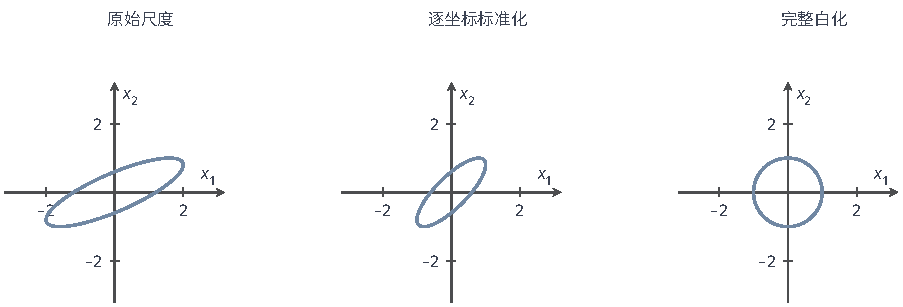
\includegraphics[width=152.834mm]{figures/03-models/02-neural-network-models/tikz/training-whitening/figure.pdf}
  \caption{以$\bm C=\left(\begin{smallmatrix}4&1.6\\1.6&1\end{smallmatrix}\right)$构造二维协方差椭圆。左图为原尺度，中图分别除以各坐标标准差，边际尺度相同但相关系数仍为0.8；右图用精确逆平方根白化后成为圆。曲线是解析示意，不是抽样散点或实验结果；忽略稳定项且不加入可学习仿射。}
  \label{fig:training-whitening}
\end{figure*}
\FloatBarrier

白化能处理逐坐标缩放保留的相关性，但协方差需要更多观测和矩阵计算，噪声方向还可能被过度放大\scite{huang2018dbn,huang2019iternorm}若将这个变换嵌入网络层，可学习仿射还可能重新引入相关性。固定输入白化使用保存的训练变换，隐藏响应若随参数改变，则需要相应网络内处理。

\paragraph{网络内的白化层。}

若希望持续处理隐藏特征之间的相关性，可以把白化嵌入网络层，但需要在前向计算协方差，并在反向处理该矩阵的依赖。\term{去相关批归一化}（DBN）采用ZCA白化，分组实现减少矩阵规模但舍去组间相关性；\term{迭代归一化}（IterNorm）用矩阵迭代近似逆平方根，避免直接特征分解。两者利用比对角标准化更完整的方向关系，也增加矩阵存储、统计误差与近似选择。这里的矩阵迭代处理协方差，与Muon对更新奇异值整形的目标不同。

\subsubsection{批归一化}
\label{sec:training-batchnorm-family}
\label{sec:training-batchnorm}
\label{sec:training-batchnorm-variants}
\label{sec:training-other-batchnorm}
\label{sec:training-batch-renorm}
\label{sec:training-online-powernorm}
\label{sec:training-conditional-norm}
\label{sec:training-temporal-batchnorm}
\label{sec:training-batch-channel-normalization}
批归一化用同一特征或通道的多个观测建立参照。相关方法围绕这一批统计机制，调整统计伙伴、训练与推理的参照、历史状态或输出仿射。

如果同一通道的整体响应尺度随训练变化，可以用共同统计伙伴提供尺度参照，并让网络学习输出幅度。代价是单个样本的计算与其他伙伴耦合，这又联系到第\ref{sec:training-inexact-gradients}节的批量组织。\term{批归一化}（batch normalization, BatchNorm）让同一特征在当前批量中的观测共同决定尺度。对全连接层$\bm X\in\mathbb R^{b\times d}$，固定特征$j$，统计$\{X_{i,j}:i=1,\ldots,b\}$；对卷积张量，固定通道$j$，再把批量与空间位置一起统计。每个特征或通道有一组$\gamma_j,\zeta_j$\scite{ioffe2015batchnorm}

以卷积通道为例，训练时计算
\begin{equation}
  \begin{aligned}
  \mu_j&=\frac1{bhw}\sum_{i,u,v}X_{i,j,u,v},\qquad
  v_j=\frac1{bhw}\sum_{i,u,v}(X_{i,j,u,v}-\mu_j)^2,\\
  Y_{i,j,u,v}&=\gamma_j\frac{X_{i,j,u,v}-\mu_j}{\sqrt{v_j+\epsilon}}+\zeta_j\text{。}
  \end{aligned}
  \label{eq:training-batchnorm}
\end{equation}
训练时用本批的$\mu_j,v_j$计算输出，所以一个样本的输出依赖其他统计伙伴。同时维护供推理使用的\term{运行均值}（running mean）和\term{运行方差}（running variance），即随训练批次更新、保存在模型中的滑动统计量。令$\rho\in[0,1)$为旧统计量的保留系数，一种更新约定为
\begin{equation}
  \begin{aligned}
    \bar\mu_j^{(t)}&=\rho\bar\mu_j^{(t-1)}+(1-\rho)\mu_j^{(t)},\\
    \bar v_j^{(t)}&=\rho\bar v_j^{(t-1)}+(1-\rho)\widetilde v_j^{(t)}\text{。}
  \end{aligned}
  \label{eq:training-batchnorm-running}
\end{equation}
这里$t$标记训练批次。式\eqref{eq:training-batchnorm}用于当前前向的$v_j^{(t)}$以$m=bhw$为分母；更新运行方差所用的$\widetilde v_j^{(t)}$则须按实现约定：可以使用同一批方差，也可以在$m>1$时使用$m v_j^{(t)}/(m-1)$。后一种在独立同分布观测下是无偏方差估计，空间相关性会改变这一性质；当前前向仍使用分母$m$的批统计。接口中的momentum可能指$\rho$，也可能指新批权重$1-\rho$，需查明定义。

采用运行统计的常规BN在推理时冻结$\bar\mu_j,\bar v_j$，既不重新计算推理批次的均值、方差，也不继续更新滑动统计；只把式\eqref{eq:training-batchnorm}中的$\mu_j,v_j$换成保存值。因而同一输入的BN输出不再随推理批次的伙伴改变。运行统计累积历次批统计，初始化、采样和训练期间的参数变化都进入这份估计；在最终参数下遍历数据得到的统计则使用另一组响应。关闭运行统计跟踪等配置会改为其他参照，实际计算由该配置决定。

若统计集合只有一个元素，中心化后为0，归一化不能保留该元素的变化。卷积中即使$b=1$，空间位置仍可提供多个元素，但高度相关的位置并不等同于独立样本。小批量、单类别采样或相邻视频帧都可能使统计量偏离预期使用分布。统计伙伴的相关性与组成决定这份尺度参照是否适合实际输入。

固定运行统计量后，BatchNorm是通道仿射变换，可与前面的线性层或卷积折叠，第\ref{sec:snn-conversion}节给出公式。训练时的批统计随输入变化，求导包含这份依赖，因此对应一张动态计算图。验证、推理和模型导出需要采用一致模式。

BatchNorm调节表示尺度，并通过重参数化影响梯度与优化形状。原始工作用内部协变量偏移说明动机，后续研究指出训练收益不能简单归因于阻止中间分布变化，在所研究设置中还体现为更平滑的优化行为。这些研究中的模型、数据与优化设置限定了所支持的解释\scite{santurkar2018batchnorm}

\paragraph{批统计范围的调整。}

批归一化的统计伙伴未必与一次参数更新使用的样本集合一致。同步与幽灵批归一化分别扩大和缩小伙伴集合，处理局部批量不足与过大统计集合的问题。分布式训练中，每台设备的局部批量可能很小。\term{同步批归一化}（synchronized BatchNorm, SyncBatchNorm）跨指定设备集合共同统计。设设备$r$有$N_r$个统计元素、均值$\mu_r$和方差$v_r$，正确合并为
\begin{equation}
  \begin{aligned}
    N&=\sum_rN_r,\qquad \mu=\frac{\sum_rN_r\mu_r}{N},\\
    v&=\frac1N\sum_rN_r[v_r+(\mu_r-\mu)^2]\text{。}
  \end{aligned}
  \label{eq:training-sync-batchnorm}
\end{equation}
设备内方差与设备间均值差共同形成合并方差，均值也按元素数加权。同步扩大伙伴并增加通信，观测间已有的相关性继续保留。大型批量检测中的同步统计是其典型使用情形\scite{peng2018megdet}

当优化批量很大，又希望保留较小统计集合时，\term{幽灵批归一化}（Ghost BatchNorm）将同一次优化批量分成较小子组，各组分别计算归一化统计，再合并梯度更新。它区分“有多少样本决定一次更新”与“有多少样本共同决定一次归一化”，两种批量分别进入前向统计和参数更新\scite{hoffer2017ghostbn}

这两种做法的优势是可以单独选择统计批量，而不必同步改变优化批量。SyncBatchNorm增加通信，Ghost BatchNorm增加统计波动；扩大或缩小伙伴都需要验证。若困难来自训练与推理参照不同，还需要下面的统计校正。

\paragraph{参照批量与训练推理校正。}

小批量或非独立采样可能使当前统计波动，训练与推理的参照又不同。相关方法通过调整参考批量或校正批统计，缓解参照差异\scite{salimans2016gantechniques,ioffe2017batchrenorm}\term{虚拟批归一化}（virtual batch normalization, VBN）将当前样本与固定参考批量结合，减少对工作批量中其他新样本的依赖；参考集合的偏差与额外计算仍会保留。这里参考批量参与前向统计，梯度累积则合并已经算出的参数导数。

\term{批再归一化}（batch renormalization）把批标准化结果改为$\hat x=r(x-\mu_B)/\sigma_B+d$。$r$由批标准差与运行标准差之比得到，$d$由两种均值之差得到，二者均按调度裁剪并停止梯度。未裁剪时，前向等于使用运行统计；反向仍通过批内统计求导。它缓解两种参照的差异，却增加运行状态和校正范围的选择。

\Needspace{18\baselineskip}
\paragraph{流式与历史统计。}

在流式或微批量条件下，\term{在线归一化}（OnlineNorm）沿样本流维护统计并设计相应的反向校正；\term{PowerNorm}用运行平方均值和近似反向处理管理Transformer中的批尺度波动\scite{chiley2019onlinenorm,shen2020powernorm}它们让参照跨时间积累，代价是状态次序、重置规则与分布变化后的滞后。前向历史与反向校正共同定义这些方法，因果预测中的统计还限制在当时已经到达的观测内。

\paragraph{条件批归一化与空间调制。}

生成任务要让共享内容表示随条件改变，固定仿射只能提供同一组尺度。\term{条件归一化}让条件$\bm c$产生$\bm\gamma(\bm c),\bm\zeta(\bm c)$，计算$\bm y=\bm\gamma(\bm c)\odot\hat{\bm x}+\bm\zeta(\bm c)$。条件化改变仿射参数的来源，底层统计伙伴仍由所选归一化决定；同一思路也可用于后面的层归一化与实例归一化。图~\ref{fig:training-conditional-norm}展示内容与条件两条路径。
\begin{figure}[htbp]
  \centering
  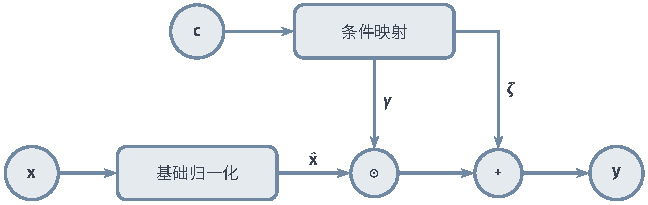
\includegraphics[width=109.792mm]{figures/03-models/02-neural-network-models/tikz/training-conditional-norm/figure.pdf}
  \caption{条件归一化的共同计算图。内容路径产生$\hat{\bm x}$，条件映射产生缩放$\bm\gamma$与偏移$\bm\zeta$，圆形节点分别表示逐元素乘法与加法。条件既可以是风格统计，也可以是类别、文本或时间等输入；空间调制还让仿射参数随位置变化。}
  \label{fig:training-conditional-norm}
\end{figure}
\FloatBarrier

条件BatchNorm保留批统计，让类别、文本等条件产生通道仿射参数。\term{空间自适应归一化}（SPADE）让语义布局产生随位置变化的缩放与偏移，把布局条件送回归一化后的特征。原工作使用同步批统计，因此在这里介绍；如果底层换为InstanceNorm，则应按实例范围理解。条件编码增加参数与计算，且仍需核对底层统计在训练和推理中的行为\scite{park2019spade}

\paragraph{时间展开的批统计。}

脉冲分布随时间变化时，\term{时间展开批归一化}（BNTT）为不同时间步设置统计与参数，使各时刻拥有相应尺度参照。它保持批归一化的统计范围，增加了时间索引，因此归入本类。代价是更多状态，推理窗口改变时还需处理未训练时刻；当前输出的统计只使用预测时已经给定的输入\scite{kim2021bntt}

\paragraph{与通道组统计和激活的组合。}

微批量下，批尺度校正还可以与样本内的通道组处理串联。\term{批通道归一化}（BCN）采用这类组合，并与参数侧的权重标准化配合。它增加了样本内统计，但保留批或历史参照的依赖；详细效果取决于统计与运行状态的实现，批/历史参照与组内计算分别进入完整模块\scite{qiao2020wsbcn}

\term{EvoNorm}把归一化与非线性共同设计。B系列使用批统计，B0还将批方差与实例方差结合，因而具有跨样本依赖，也需维护推理统计。它与先BatchNorm再激活的计算不同；替换时需核对整个模块。使用样本内组统计的S0放在第\ref{sec:training-groupnorm}节介绍\scite{liu2020evonorm}

\subsubsection{层归一化}
\label{sec:training-layernorm-family}
\label{sec:training-layernorm}
\label{sec:training-rmsnorm}
\label{sec:training-scalenorm}
\label{sec:training-pixelnorm}
\label{sec:training-qknorm}
\label{sec:training-adaptive-layernorm}
\label{sec:training-normalization-block-designs}
\label{sec:training-normalization-placement}
\label{sec:training-other-normalization-designs}
这一类在单个样本的指定表示内部建立尺度参照，不借用其他样本。相关方法保留这一作用范围，改变是否中心化、如何计算长度以及仿射参数的来源；层归一化在残差块中的放置方式也在本类内说明。

批量组成或大小变化时，跨样本参照可能不适合当前表示。LayerNorm把尺度参照移到同一个样本表示内部，隔离其他样本对这一步局部导数的影响。逐词元计算也让参照范围不随序列长度和推理批量改变。\term{层归一化}（layer normalization, LayerNorm）对选定表示中的多个特征共同计算均值与方差。对$\bm X\in\mathbb R^{b\times n\times d}$，Transformer通常固定样本$i$与词元位置$t$，在特征维$j=1,\ldots,d$上统计，使用式\eqref{eq:training-normalization-common}，仿射参数$\bm\gamma,\bm\zeta\in\mathbb R^d$跨样本和位置共享\scite{ba2016layernorm}

其他样本和其他位置不参与当前词元的统计，训练与推理均使用当前表示。因此，逐词元LayerNorm不依赖批量组成，也不需要保存运行均值与方差。注意力、池化和损失再用各自掩码处理有效位置，LayerNorm在每个位置内部统计。

层归一化的实际范围由选定形状规定。对图像，可以选定全部通道及空间位置，也可以只在每个位置跨通道统计；两种形状会保留不同信息。整样本LayerNorm的仿射参数还可能逐元素设置，GroupNorm则通常逐通道设置，即使统计范围相同也未必是同一个完整映射。

若忽略$\epsilon$，对$\bm x$加同一个常数或乘以同一个正数，不改变中心化后的标准化表示。它消去的是共同平移与尺度，保留相对特征关系。若任务需要共同幅值，应依靠保留路径或其他设计保存，固定$\gamma,\zeta$只规定公共仿射，逐输入被消去的幅度需要由其他路径提供。

\paragraph{均方根归一化。}

式\eqref{eq:training-normalization-jacobian}中的中心化会消去共同平移方向；如果只想管理幅度，这一步未必必要。RMSNorm保留未中心化表示，再由平方幅度决定尺度。\term{均方根归一化}（root mean square normalization, RMSNorm）对$\bm x\in\mathbb R^d$采用
\begin{equation}
  y_j=\gamma_j\frac{x_j}{\sqrt{d^{-1}\sum_{k=1}^d x_k^2+\epsilon}}\text{。}
  \label{eq:training-rmsnorm}
\end{equation}
基本形式不减均值，也不加入偏移参数。它使表示对共同正尺度变化近似不敏感，但不对共同平移不敏感；分母同时包含方差与均值平方，因为$d^{-1}\sum_jx_j^2=v+\mu^2$\scite{zhang2019rmsnorm}

\begin{example}[减去均值改变了哪些信息]
  \label{ex:training-layer-rms}
  取两个仅相差共同偏移的向量：
  \[
    \bm x=(1,2,3)^{\top},\qquad \bm x'=(11,12,13)^{\top}\text{。}
  \]
  忽略$\epsilon$并令仿射缩放为1，LayerNorm的两次输出都为
  \[
    (-\sqrt{3/2},0,\sqrt{3/2})^{\top}\text{。}
  \]
  共同偏移10被消去。RMSNorm分别给出$\bm x/\sqrt{14/3}$与$\bm x'/\sqrt{434/3}$，结果不同。二者都控制尺度，但保留的信息不同。
\end{example}

RMSNorm省去中心化与偏移，统计操作较少，并保留共同偏移对方向和分母的影响；共同正缩放在忽略稳定项时仍被消去，原始幅度因而需要另行保存。是否比LayerNorm更适合，应结合任务需要的信息与实际算子成本判断。

\paragraph{部分统计与整体长度。}

\term{部分RMSNorm}（pRMSNorm）只用特征子集估计均方根，以减少统计量的归约计算。节省来自少统计一些元素，风险是子集不能代表完整幅度，算子实现也决定它是否实际更快。

有些任务关心向量方向，或希望仅管理局部响应的幅度。\term{ScaleNorm}采用$\bm y=g\bm x/\max(\lVert\bm x\rVert_2,\epsilon)$，只学习一个整体长度$g$；\term{FixNorm}固定嵌入长度，普通L2归一化则得到单位向量。它们计算简单，适合将方向用于相似性，但会删除绝对幅度；逐特征可学习缩放与整体长度并不等价\scite{nguyen2019scalenorm}

\paragraph{图像位置与注意力向量的长度。}

\term{PixelNorm}在单个图像位置跨通道计算均方根，基本形式没有仿射与中心化；PGGAN用它管理生成器特征幅度。按统计范围，它与逐位置RMS缩放相近，所以放在层内特征尺度方法中；其统计只覆盖当前空间位置的通道，原始幅度仍受该缩放影响\scite{karras2018pggan}

\term{查询--键归一化}（QKNorm）在每个注意力头内归一化单个查询和键向量的长度，以可学习系数缩放余弦得分。它同样只处理当前向量的特征维，目的是减少长度增长引起的Softmax饱和。它管理注意力评分的尺度，残差块的表示统计属于另一条路径，查询键归一化之后还需配置评分温度\scite{henry2020qknorm}

\paragraph{条件层归一化。}

当输出需要随类别、文本或时间等条件变化时，\term{自适应LayerNorm}（AdaLN）在层统计之后使用条件仿射，条件RMSNorm则保留均方根统计。二者沿用图~\ref{fig:training-conditional-norm}的两条路径，改变的是仿射来源。DiT中的AdaLN-Zero还把残差条件门初始化为0，让初始分支较弱；“Zero”指门与相应仿射的初始化，训练会继续调整这些参数。底层统计、条件网络与残差门须分别说明\scite{peebles2023dit}

\paragraph{残差块中的放置与尺度配合。}

层归一化的统计范围不变，放置位置与残差尺度仍会改变第\ref{sec:training-gradient-propagation}节的Jacobian矩阵连乘\scite{shleifer2021normformer,wang2022deepnet}Pre-LN残差块形如$\bm h'=\bm h+F(\operatorname{LN}(\bm h))$，Post-LN形如$\bm h'=\operatorname{LN}(\bm h+F(\bm h))$。前者保留未经过本步归一化的直接路径，后者对合并结果共同归一化；输出尺度、梯度路径和初始化需求不同，第\ref{sec:transformer-residual-normalization}节展开了具体结构。

直接路径有利于把梯度送回较早层，但Pre-LN分支仍可能很弱，整体尺度仍需管理；Post-LN约束合并后的表示，却让归一化导数进入每个块的传播。选择位置应配合残差尺度与初始化。

NormFormer增加归一化位置与尺度调节，DeepNorm配合残差缩放和初始化支持更深堆叠；二者通过完整块组织、残差系数和初始参数共同作用于传播。增加操作或改变系数也有成本，应检查完整计算图与初始化条件。

\subsubsection{实例归一化}
\label{sec:training-instancenorm}
\label{sec:training-adaptive-instancenorm}
\label{sec:training-frn-pixelnorm}
\label{sec:training-frn}
图像外观可能随样本变化，共享批统计未必能去掉每幅图各通道的独有尺度。InstanceNorm在该样本通道内部建立参照，代价是可能同时去掉有用的外观幅度。图像中，某个通道的均值与对比度可能更多描述风格，而非内容。\term{实例归一化}（instance normalization, InstanceNorm）固定样本$i$和通道$j$，只在$(u,v)$上计算均值与方差。常见实现不使用跨样本运行统计，训练与推理都归一化当前输入；可选仿射参数按通道共享\scite{ulyanov2016instancenorm}

它把每个样本的每个通道都调整到相近统计尺度，有利于去除某些外观差异，却也可能消去任务需要的亮度或强度。若空间只剩一个元素，中心化会退化；若启用运行统计，推理性质又不同。空间形状、仿射参数与运行统计配置共同确定这张映射。

\paragraph{自适应实例归一化。}

若希望内容保留空间结构，同时采用另一幅图的通道统计，可以在实例标准化后重设均值与幅度。\term{自适应实例归一化}（AdaIN）用风格特征的通道均值和标准差重设内容统计，形式为$\sigma(\bm s)\odot[\bm x-\mu(\bm x)]/\sigma(\bm x)+\mu(\bm s)$，零方差需稳定处理。它保留实例统计范围，把固定仿射换为风格统计；这种匹配方便注入外观条件，感知风格的相似程度还由后续生成与评价确定\scite{huang2017adain}

\paragraph{不减均值的滤波响应归一化。}

如果希望在每个样本的每个通道内管理幅度，又保留共同偏移的影响，可以在相同空间范围内改用未中心化的平方幅度。\term{滤波响应归一化}（FRN）沿这一范围计算均方根，不减均值，再使用仿射和可学习阈值激活。按作用范围将它放在本类，但它与标准InstanceNorm的映射不同；完整模块还包含激活，空间很小时稳定项与信息损失尤须注意\scite{singh2020frn}

\subsubsection{组归一化}
\label{sec:training-groupnorm}
\label{sec:training-instance-groupnorm}
\label{sec:training-evonorm}
统计集合太小会使尺度估计不稳定，全部通道混合又可能过于粗糙。GroupNorm在样本内部选择中间大小的通道组，在信息粒度与统计元素数之间取舍。\term{组归一化}（group normalization, GroupNorm）将$c$个通道预先划为$g$组，在单个样本内对组内通道及空间位置共同统计。等分时要求$c$能被$g$整除，每组统计元素数为$(c/g)hw$，仿射参数通常仍逐通道设置\scite{wu2018groupnorm}

当$g=c$时，统计范围与InstanceNorm相同；当$g=1$时，与整样本LayerNorm相同。完整映射仍需核对仿射参数和运行统计配置。组数控制哪些特征共同决定尺度，相应组数与任务信息、形状和训练共同决定输出表现。

\paragraph{组统计与非线性的联合计算。}

组归一化后再接激活，会让两步导数共同进入反向传播。上文EvoNorm系列中的S0直接联合这两部分，采用$y_j=\gamma_jx_j\sigma(a_jx_j)/\sqrt{v_G+\epsilon}+\zeta_j$，其中$v_G$是样本内通道组的中心化方差，$a_j$可学习，$\sigma$为Sigmoid。它使用组统计，分子却不减均值，中心化分母与未中心化分子共同形成这一模块，另接同样激活又会改变其输出和导数。

图~\ref{fig:training-normalization-axes}用同一构造数据比较已讨论的批、层、实例和组统计。图中采用常见轴名$N,C,H,W$，分别对应前文的批量$b$、通道$c$、高$h$和宽$w$；元素索引写作$(n,c,h,w)$。图将$(h,w)$展开为行、通道$c$排成列，两张小表分别表示样本$n=1,2$。轮廓内的着色格共同计算均值与方差，圈出的目标元素始终不变，因而可以直接比较哪些伙伴被加入或排除。

BN固定$c$，跨$n,h,w$统计；IN固定$n,c$，只跨$h,w$，并不跨实例。GN固定$n$和通道组，跨组内$c$及$h,w$。图中的LN明确采用图像整样本约定：固定$n$，统计全部$C,H,W$。Transformer的逐词元LN则固定样本$n$和词元位置$t$，只沿特征$C$（前文记为$d$）统计；序列中的统计伙伴因而与图示整幅图像不同。选择统计伙伴改变数值结果，也改变式\eqref{eq:training-normalization-jacobian}中哪些特征共同参与导数。
\begin{figure*}[htbp]
  \centering
  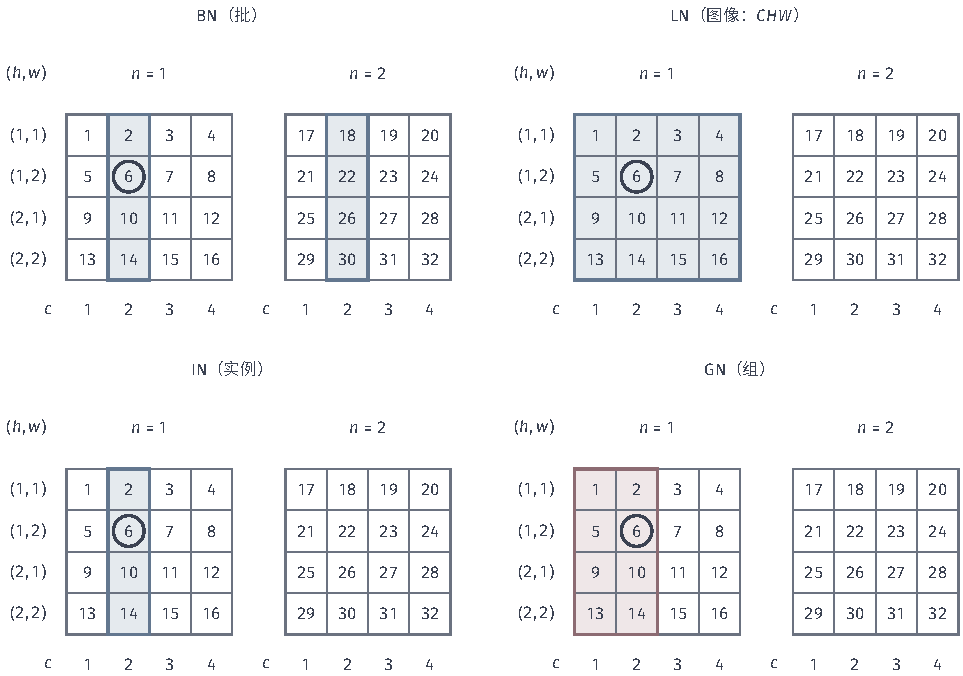
\includegraphics[width=163.146mm]{figures/03-models/02-neural-network-models/tikz/training-normalization-axes/figure.pdf}
  \caption{在$N=2,C=4,H=W=2$的图像张量上，对同一元素$X_{1,2,1,2}=6$比较统计伙伴。按样本、空间行、通道的展示顺序填入教学数值1至32，每行标出$(h,w)$；并非按张量存储顺序编号。蓝、紫、青、橙分别标出BN、LN、IN、GN的统计集合，边界轮廓及$n$、$c$、$(h,w)$标签提供颜色之外的读法，深色圈为目标元素。GN取通道组$\{1,2\}$；LN统计整幅图像的$CHW$，不是Transformer逐词元的特征维LN；图中未加入仿射变换。}
  \label{fig:training-normalization-axes}
\end{figure*}
\FloatBarrier

表~\ref{tab:training-normalization-axes}将范围写成索引，便于在不同张量排列下实现。位置、通道和批量放在第几个维度可以改变，但统计伙伴的语义必须保持。
\begin{table*}[htbp]
  \centering\small
  \begin{tabularx}{\linewidth}{@{}p{35mm}p{43mm}X@{}}
    \toprule
    方法 & 固定的索引 & 共同计算统计量的索引 \\
    \midrule
    BatchNorm & 通道$j$ & 样本$i$、位置$u,v$ \\
    LayerNorm（整样本） & 样本$i$ & 通道$j$、位置$u,v$ \\
    LayerNorm（每位置） & 样本$i$、位置$u,v$ & 通道$j$ \\
    InstanceNorm & 样本$i$、通道$j$ & 位置$u,v$ \\
    GroupNorm & 样本$i$、通道组 & 组内通道$j$、位置$u,v$ \\
    \bottomrule
  \end{tabularx}
  \caption{在$\bm X\in\mathbb R^{b\times c\times h\times w}$上比较基本统计范围。每位置LayerNorm与序列中的逐词元形式对应；整样本形式与$g=1$的GroupNorm仅在统计范围上相同。RMSNorm也需明确形状，但统计的是平方均值而非中心化方差。}
  \label{tab:training-normalization-axes}
\end{table*}
\FloatBarrier

\subsection{参数归一化}
\label{sec:training-parameter-normalization-methods}
\label{sec:training-weight-normalization-methods}
前面的基本方法管理表示统计，权重方法则直接改变线性映射的参数化。权重自身提供尺度参照，向量长度、滤波器均值方差和整矩阵最大放大分别对应不同约束。

\subsubsection{权重归一化}
\label{sec:training-weightnorm}
第\ref{sec:training-curvature}节指出重参数化可以改变更新几何。WeightNorm把长度与方向作为不同变量，让优化器分别调整两种自由度，无需估计激活的批统计。\term{权重归一化}（weight normalization, WeightNorm）把非零权重向量写为
\begin{equation}
  \bm w=g\frac{\bm v}{\lVert\bm v\rVert_2}\text{，}
  \label{eq:training-weightnorm}
\end{equation}
其中$g$是可训练标量，$\bm v$决定方向。对卷积可按输出滤波器分别使用，对线性层可按行使用。这份方向/长度参数化由权重决定，激活均值继续取决于输入与映射\scite{salimans2016weightnorm}

设原权重梯度为$\bm a=\nabla_{\bm w}\mathcal L$，链式法则给出$\partial\mathcal L/\partial g=\bm v^{\top}\bm a/\lVert\bm v\rVert_2$，以及
\begin{equation}
  \nabla_{\bm v}\mathcal L
  =\frac{g}{\lVert\bm v\rVert_2}
    \left(\bm I-\frac{\bm v\bm v^{\top}}{\lVert\bm v\rVert_2^2}\right)\bm a\text{。}
  \label{eq:training-weightnorm-gradient}
\end{equation}
方向梯度包含垂直投影，因此更新$g,\bm v$与直接更新$\bm w$的轨迹不同。$\bm v=\bm0$需要由初始化和数值处理避免。行长度与整矩阵最大放大还具有不同口径：例如两行都为$(1,0)$时，矩阵谱范数为$\sqrt2$，超过单行长度1。

\subsubsection{权重标准化}
\label{sec:training-weight-standardization}
滤波器自身的均值和尺度会影响初始及后续响应，批量很小时也难以依靠稳定批统计补偿。WS直接处理权重分布，使这一尺度管理与当前样本伙伴分开。\term{权重标准化}（weight standardization, WS）不只分离长度，还对每个滤波器的权重减均值并按标准差缩放。将第$i$个输出滤波器展平为$d$个元素，采用
\begin{equation}
  \begin{aligned}
    \mu_i^W&=\frac1d\sum_jW_{i,j},\qquad
    v_i^W=\frac1d\sum_j(W_{i,j}-\mu_i^W)^2,\\
    \bar W_{i,j}&=\frac{W_{i,j}-\mu_i^W}{\sqrt{v_i^W+\epsilon}}\text{。}
  \end{aligned}
  \label{eq:training-weight-standardization}
\end{equation}
实际卷积使用$\bar{\bm W}$，反向穿过权重统计更新原始$\bm W$。它管理的是滤波器参数分布，与在样本或位置上统计的GroupNorm可以组合。微批量训练中的WS与BCN研究了这类互补作用，权重与样本统计分别改变映射的不同环节\scite{qiao2020wsbcn}

WS控制滤波器统计，输出激活则继续依赖输入与空间结构。

\paragraph{缩放权重标准化。}

带增益和扇入校正的缩放权重标准化继续作用于滤波器参数。NFNet把它与残差信号尺度、激活修正和自适应梯度裁剪配合，以减少通常的激活批统计依赖。这些尺度、连接与裁剪共同构成完整模型，实验中的收益对应这组设计\scite{brock2021nfnet}

\subsubsection{谱归一化}
\label{sec:training-spectralnorm}
激活方差或每行长度并不控制所有方向的最大放大。第\ref{sec:training-gradient-propagation}节使用的算子上界，需要与最大奇异值相关的控制，谱归一化因此关注线性映射的最大放大。\term{谱归一化}（spectral normalization）对非零矩阵采用$\bar{\bm W}=\bm W/\sigma_{\max}(\bm W)$，$\sigma_{\max}$为最大奇异值。计算中常以幂迭代近似：交替用$\bm W^{\top}\bm u$与$\bm W\bm v$并归一化，再估计$\bm u^{\top}\bm W\bm v$\scite{miyato2018spectral}

若估计值小于真实最大奇异值，除法后的真实算子范数仍可能超过1，严格的算子上界需要控制这份估计误差。零矩阵与很小估计还需稳定处理，是否沿估计向量求导也应按实现说明。

若每层算子范数已受约束，且激活是已知Lipschitz映射，普通串联网络的输入敏感度可由尺度乘积控制。残差求和、归一化和注意力需另行计入。卷积核展平矩阵的谱范数与完整空间卷积算子通常不同，整网敏感度应据实际卷积算子及其他模块合计。谱归一化控制最大方向，WeightNorm分离方向与长度，WS调整滤波器均值和方差，三者目的不同。

\subsection{其他归一化方法}
\label{sec:training-other-normalization}
有些方法混合多个统计范围，有些围绕可逆变换、图结构或通道竞争定义尺度，这些计算使用的对象或范围超出了前述基本形式。这里按具体计算作补充；是否采用仍要对应实际训练困难，并评估信息损失、状态与计算成本。

\subsubsection{混合统计与局部响应}
\label{sec:training-normalization-combinations}
\label{sec:training-switchable-bcn}
固定统计范围未必适合每一层。\term{可切换归一化}（SwitchableNorm）分别计算批、层、实例统计，学习均值和方差的凸组合。它同时使用多个范围，因而不放入单一基础类别。统计混合增加计算，只要批分量存在，就仍需处理跨样本或历史依赖；这与第\ref{sec:training-batchnorm-family}节中BCN串联不同，后者依次执行映射\scite{luo2019switchablenorm}

\term{局部响应归一化}（local response normalization, LRN）属于局部除法竞争。第\ref{sec:cnn-alexnet}节中AlexNet的一种形式为$y_j=x_j/(k_0+a\sum_{r\in N(j)}x_r^2)^\beta$，这里省略样本与空间索引，$N(j)$是邻近通道，$k_0>0,a\geq0,\beta>0$。强响应会抑制邻域幅度；它既不减均值，也不按前述批、层、实例或固定通道组计算标准差，它形成了另一种局部响应函数。

\subsubsection{可逆仿射}
\label{sec:training-actnorm}
可逆生成模型需要逐样本可逆、且行列式容易计算的尺度变换。\term{ActNorm}用首批数据初始化通道仿射$Y_{i,j,u,v}=s_jX_{i,j,u,v}+b_j$，之后直接学习$s_j,b_j$，不再重估每批统计。取$s_j=\exp(a_j)$可保证非零尺度；单样本对数Jacobian行列式为$hw\sum_j\log|s_j|$。其优势是逐样本计算一致、可逆性明确，代价是初始数据影响起点，后续输出不再保证零均值和单位方差\scite{kingma2018glow}

\subsubsection{通道响应与图结构}
\label{sec:training-grn-qknorm}
\label{sec:training-graph-temporal-norm}
\label{sec:training-global-response-normalization}
\term{全局响应归一化}（GRN）在ConvNeXt V2中比较各通道的空间L2响应，再将相对强度用于残差调制。它管理通道竞争，不强制单位方差；其映射同时使用空间响应与通道间的相对比较\scite{woo2023convnextv2}

图模型的统计还需尊重每张图的边界。\term{GraphNorm}逐图、逐特征统计，以可学习系数决定去掉多少图均值；\term{PairNorm}中心化节点后统一缩放总体长度，管理节点间距离；\term{MessageNorm}把聚合消息的长度调整为相对节点状态的可学习比例。它们分别处理图级偏移、过平滑与消息幅度，各自参照图均值、节点距离或消息相对长度\scite{cai2021graphnorm,zhao2020pairnorm,li2020deepergcn}

这些方法分别调整保留下来的图偏移、节点距离或消息幅度。图边界与节点分布、节点间差别、消息与状态的相对长度，因而成为各自的诊断对象；任务表现再显示这些调整是否适合当前预测。

\subsubsection{统计归一化的替代}
\label{sec:training-normalization-substitutes}
尺度也可以由不使用样本统计的非线性压缩管理。2025年的\term{动态Tanh}（DyT）以$\bm\gamma\odot\tanh(a\bm x)+\bm\zeta$替代部分Transformer归一化层，不计算当前表示的均值或方差，因此不能按前述统计范围归类。它展示了另一种尺度控制路线，也要求保留其配套设计和实验范围；替换效果对应论文中的模块、配套设置与任务\scite{zhu2025dyt}

\subsection{归一化方法的比较与选择}
\label{sec:training-normalization-comparison}
比较方法时，可以回到第\ref{sec:training-curvature}节的方向尺度与第\ref{sec:training-gradient-propagation}节的Jacobian矩阵连乘。特征归一化改变输入或隐藏表示，参数归一化改变生成映射的权重；二者可能共同改善尺度，但即使输出方差相近，统计依赖与参数化仍可产生不同导数。选择时需同时检查以下维度：
\begin{itemize}
  \item \textbf{作用对象。} 调整的是输入、隐藏特征还是权重，决定直接改变计算图的哪一部分。
  \item \textbf{统计范围。} 跨样本、表示内部、单通道空间或通道组，决定计算依赖和统计元素数；白化还需估计特征间的协方差。
  \item \textbf{保留信息。} 是否去均值、固定长度或去相关，决定共同偏移、幅度与方向关系怎样改变。
  \item \textbf{执行条件。} 固定训练参照、当前统计还是运行状态，决定训练推理是否一致，以及通信、矩阵计算和条件网络的成本。
\end{itemize}

表~\ref{tab:training-normalization-basic-comparison}比较五类特征方法，表~\ref{tab:training-normalization-special-comparison}比较参数方法，表~\ref{tab:training-normalization-extended-comparison}列出具体方法的归属。分类先固定作用对象和统计范围，再比较范围内的公式差异；条件仿射与残差块位置属于相应基础方法的扩展，不另列为一种统计类别。
\begin{table*}[htbp]
  \centering\small
  \begin{tabularx}{\linewidth}{@{}p{24mm}p{43mm}p{35mm}X@{}}
    \toprule
    类别 & 统计或尺度对象 & 主要处理 & 优势与主要边界 \\
    \midrule
    白化 & 观测集合内的特征协方差 & 中心化与协方差变换 & 去相关；矩阵计算与统计误差较大 \\
    批归一化 & 同通道的批量与空间位置 & 批均值、方差或历史尺度 & 共享尺度参照；批伙伴与推理状态需核对 \\
    层归一化 & 单表示的指定特征维 & 方差、均方根或向量长度 & 隔离其他样本；变体保留的信息不同 \\
    实例归一化 & 单样本单通道的空间位置 & 方差或未中心化平方幅度 & 管理样本外观；可能删去有用强度 \\
    组归一化 & 单样本组内通道与空间位置 & 组内统计 & 不依赖批量；组数改变信息粒度 \\
    \bottomrule
  \end{tabularx}
  \caption{按作用范围比较特征归一化。白化可采用训练集固定参照或网络内动态协方差；批归一化通常在推理时使用运行统计。其余类别按基本形式使用当前表示，具体变体还需核对中心化、仿射与状态。}
  \label{tab:training-normalization-basic-comparison}
\end{table*}
\FloatBarrier

\begin{table*}[htbp]
  \centering\small
  \begin{tabularx}{\linewidth}{@{}p{31mm}p{51mm}X@{}}
    \toprule
    方法 & 管理的参数性质 & 优势与主要边界 \\
    \midrule
    WeightNorm & 分开权重方向与长度 & 不需批统计；行长度不控制整矩阵谱范数 \\
    WS及缩放变体 & 滤波器均值与方差、增益与扇入尺度 & 与激活统计分开；不保证输出尺度 \\
    SpectralNorm & 最大奇异值 & 管理最大线性放大；近似及算子定义需明确 \\
    \bottomrule
  \end{tabularx}
  \caption{参数归一化的比较。三者不依赖当前批量，但重参数化或归一化改变优化轨迹；缩放WS还需核对具体结构中的配套系数。}
  \label{tab:training-normalization-special-comparison}
\end{table*}
\FloatBarrier

\begin{table*}[htbp]
  \centering\small
  \begin{tabularx}{\linewidth}{@{}p{26mm}p{85mm}X@{}}
    \toprule
    归属 & 方法与相关扩展 & 需要单独核对的改动 \\
    \midrule
    特征：白化 & ZCA、DBN、IterNorm & 固定或当前协方差、分组与矩阵近似 \\
    特征：批归一化 & BatchNorm；Sync／Ghost BN、VBN、Batch Renorm、OnlineNorm、PowerNorm、BNTT；条件BN、SPADE、BCN、EvoNorm-B & 伙伴、运行状态、时间索引、条件仿射或联合模块 \\
    特征：层归一化 & LayerNorm；RMSNorm、pRMSNorm、ScaleNorm、FixNorm、PixelNorm、QKNorm；AdaLN、条件RMSNorm；Pre／Post-LN、NormFormer、DeepNorm & 中心化与长度、条件来源、评分尺度和块位置 \\
    特征：实例归一化 & InstanceNorm、AdaIN、FRN & 风格统计、均方根与阈值激活 \\
    特征：组归一化 & GroupNorm、EvoNorm-S0 & 组数与联合非线性 \\
    参数归一化 & WeightNorm、WS、缩放WS、SpectralNorm & 重参数化、增益与算子尺度 \\
    其他方法 & SwitchableNorm、LRN、ActNorm、GRN、GraphNorm、PairNorm、MessageNorm、DyT & 混合范围、局部竞争、可逆性、图边界或替代统计 \\
    \bottomrule
  \end{tabularx}
  \caption{具体方法的归属对照。前五行对应第\ref{sec:training-feature-normalization-methods}节的五类，参数方法见第\ref{sec:training-parameter-normalization-methods}节，其他方法见第\ref{sec:training-other-normalization}节。共同范围内仍有公式与模块差异；SPADE的底层统计可配置，BCN含串联组统计，Pre／Post-LN等是层归一化的组织方式，DyT是替代方案。}
  \label{tab:training-normalization-extended-comparison}
\end{table*}
\FloatBarrier

实际选择从任务信息与执行条件出发。输入量纲差异可先用固定标准化处理，需要去相关时再评估白化及矩阵成本；卷积中批伙伴足够且推理运行统计可靠时，可评估BatchNorm；批量很小或组成经常改变时，可比较GroupNorm及其组数。逐词元序列表示可在层内比较LayerNorm与RMSNorm，重点核对中心化是否有益；需要管理每幅图的通道外观时，再评估InstanceNorm与条件扩展。

若目标是控制线性映射的最大放大，参数侧的谱尺度给出相应方向指标，特征方差则描述指定输入下的响应。条件、混合与特殊结构方法也应在出现对应困难后引入，并在同一数据、结构与预算下检验收益及额外成本。

\section{参数与结构的改进}
\label{sec:training-connections}

优化器处理已经产生的梯度，参数与结构的设计则决定梯度怎样形成、从哪里传回。第\ref{sec:training-gradient-propagation}节的连乘关系说明：已经在连乘中衰减的信号，需要在相应路径与因子上处理。残差、门控与跨层连接改变计算路径，初始化决定出发时的信号尺度，持续参数约束则管理训练过程中允许的映射。这些选择沿训练轨迹共同形成实际更新。

\subsection{残差连接}
\label{sec:training-residual}

式\eqref{eq:training-jacobian-chain}中若每步都只能经过可学习变换，任何一步的方向收缩都会进入长乘积。\term{残差连接}（residual connection）在可学习变换外增加直接路径，让梯度有机会绕过变换分支。设输入输出同维，写为
\begin{equation}
  \bm h^{(l+1)}=\bm h^{(l)}+a_lF_l(\bm h^{(l)}),\qquad
  \bm J_{l+1}=\bm I+a_l\bm J_{F_l}\text{。}
  \label{eq:training-residual-jacobian}
\end{equation}
其中$a_l$为分支尺度，$\bm J_{F_l}$为分支Jacobian矩阵。原来的纯变换连乘改为含恒等项的连乘；分支在初始阶段较小时，网络可以从接近恒等映射的状态开始学习调整。直接支路改变传播路径，分支尺度再控制新增变换的强度。

恒等项与分支导数相加后，仍可能发生抵消或累积放大。若$a_l\bm J_{F_l}=-\bm I$，一层Jacobian矩阵仍可为0；若每层都沿同一方向放大，连乘仍可能增长。一个粗上界为$\prod_l(1+|a_l|\lVert\bm J_{F_l}\rVert_2)\leq\exp(\sum_l|a_l|\lVert\bm J_{F_l}\rVert_2)$，它说明分支尺度和总深度需要共同考虑。初始化、归一化与尺度方案据各分支导数及其组合共同分析。

当维度改变时，路径写为$\bm P_l\bm h^{(l)}+F_l(\bm h^{(l)})$，投影$\bm P_l$代替恒等矩阵。下采样和投影可能丢失部分方向，因而需区别恒等捷径与投影捷径。第\ref{chap:convolutional-networks}章的ResNet与第\ref{chap:transformer}章的残差块均是这一框架的具体组织。

\subsection{门控连接}
\label{sec:training-gates}

恒等捷径以固定系数传递输入，其保留比例与当前内容无关。\term{门控连接}（gated connection）把路径系数变成输入相关变量，在保留原状态与使用新计算之间调节比例。一个耦合门形式为
\begin{equation}
  \bm h^{(l+1)}=(\bm1-\bm g_l)\odot\bm h^{(l)}
                   +\bm g_l\odot F_l(\bm h^{(l)}),
  \qquad\bm g_l=\sigma(G_l(\bm h^{(l)}))\text{。}
  \label{eq:training-gated-connection}
\end{equation}
门接近0时主要保留输入，接近1时主要使用新计算。Highway网络在深度方向采用此类选择，LSTM的遗忘门和输入门则在时间方向分别控制保留与写入；这些门可以独立，不一定总和为1。GRU的更新门在旧状态与候选状态之间调节比例，重置门控制候选计算对历史的使用。

把门视为当前固定值时，保留项的局部导数为$\operatorname{diag}(\bm1-\bm g_l)$。如果门依赖输入，完整Jacobian矩阵还包含$\operatorname{diag}(F_l(\bm h)-\bm h)\bm J_{g_l}$，门的变化因而也是完整导数的一部分。时间方向上，长段保留门的乘积仍可能衰减；门长期饱和还会使门参数自身难学。初始化门偏置可以改变初始保留倾向，但是否有利取决于所需记忆长度和写入需求。

\subsection{跨层连接与密集连接}
\label{sec:training-dense-connections}

深层信息不一定都应经逐层压缩后才被使用。跨层连接给后续变换直接读取早期特征的入口，同时为反向建立较短路径；拼接再决定这些信息是否保留独立坐标。残差相加要求两路表示在对应坐标上合并。跨层拼接则把来自不同层的表示同时交给后续计算。\term{密集连接}（dense connection）令第$l$层读取之前多层的特征，例如
\begin{equation}
  \bm h^{(l)}=F_l([\bm h^{(0)};\bm h^{(1)};\cdots;\bm h^{(l-1)}])\text{，}
  \label{eq:training-dense-concat}
\end{equation}
分号表示沿特征维拼接。早期特征可经较短路径进入后面层，且保留独立坐标；后续层再学习使用哪些信息。第\ref{chap:convolutional-networks}章的DenseNet通过增长率与过渡层控制通道规模。

相加不会仅因合并而增加宽度，拼接会增加宽度与激活存储。若每层新增$k$维特征，初始宽度为$d_0$，第$l$层输入宽度为$d_0+(l-1)k$；在每层采用完整线性投影到$k$维的简化模型中，总权重数为$\sum_l k[d_0+(l-1)k]=O(Lkd_0+L^2k^2)$。真实卷积、瓶颈和过渡层改变常数及规模，参数预算据这些实际宽度和投影计算。

较长的跳跃连接也可把编码器的高分辨率特征交给解码器，减少信息必须经过压缩瓶颈的程度。连接提供了可用路径，模型是否利用它仍取决于后续变换和训练目标；错误的尺寸对齐或相加语义会破坏这一作用。训练时还需保存所引用的激活，较短传播路径与所引用表示的存储分别产生便利和代价。

\subsection{参数初始化}
\label{sec:training-initialization-constraints}
\label{sec:training-initialization}

在第\ref{sec:training-gradient-propagation}节的连乘尚未被数据更新改变前，初始权重已经决定信号是否容易传播。初始化通过打破对称和安排尺度，为后续优化提供可用起点。全零初始化使同层对称单元收到相同信号，随机初始化打破对称性；尺度过大或过小，又可能让表示与梯度迅速放大或衰减。\term{方差保持初始化}（variance-preserving initialization）按输入输出连接数与激活特性设置随机权重尺度，目的是在近似独立、零均值等假设下保持前向或反向的平均平方幅度。

对线性或近似线性激活，常见Xavier尺度为$\operatorname{Var}(W_{i,j})=2/(d_{\mathrm{in}}+d_{\mathrm{out}})$；对ReLU前向传播，He尺度为$2/d_{\mathrm{in}}$。后者中的2补偿对称输入下ReLU约保留一半平方幅度的效应。卷积中的$d_{\mathrm{in}}$要计入核位置与输入通道；分组连接、残差求和和门控则需按实际结构修正。逐层方差推导见第\ref{chap:feedforward-networks}章\scite{he2015rectifiers}

\term{正交初始化}（orthogonal initialization）令方阵权重满足$\bm W^{\top}\bm W=\bm I$，线性映射保持欧氏范数；矩形权重则只能在相应子空间或行、列方向具有类似性质。\term{恒等初始化}（identity initialization）将适当的方阵设为单位矩阵，让初始线性路径直接传递状态。两者只约束初始权重，后续无约束更新会改变这些性质，非线性激活也会改变整体Jacobian矩阵。

初始参数梯度及其核矩阵描述最初可用的学习方向，起点因此影响的不仅是激活方差（参考\BookSectionRef{sec:neural-tangent-kernel}{第二卷“基础、理论和可信性”的“深度学习的可学习性”章“基于参数梯度初始值的可学习性”节}）。有限宽度网络的参数移动可能改变核与谱，训练中的实际性质再沿更新轨迹分析。

\subsection{参数约束}
\label{sec:training-parameter-constraints}

初始化改善出发时的传播，无约束更新却可能逐渐破坏它。若希望训练期间持续限制线性映射，可通过投影、结构化参数化或惩罚维持约束。这对应第\ref{sec:training-gradient-propagation}节中每一步Jacobian矩阵尺度的管理，而不是仅在第0步选择一个矩阵。

约束要写进参数生成或更新过程。暂定更新不满足硬约束时，投影会把它改成可行参数；结构化参数化从一开始就生成可行矩阵；惩罚则允许暂时甚至持续违反，只通过损失和梯度增加代价。三者分别修正暂定值、生成可行值或改变更新目标，下面沿这三个过程展开。

\subsubsection{先更新，再投影回可行集合}

设允许的参数集合为非空闭集$\bm C$，先由优化器算出暂定值$\tilde{\bm\theta}^{(t)}$，再取
\begin{equation}
  \bm\theta^{(t)}\in\argmin_{\bm z\in\bm C}
    \tfrac12\lVert\bm z-\tilde{\bm\theta}^{(t)}\rVert_2^2\text{。}
  \label{eq:training-parameter-projection}
\end{equation}
这一步寻找距离暂定值最近的可行点。闭凸集合的欧氏投影唯一，非凸集合可能存在多解。对半径$r>0$的范数球$\bm C=\{\bm w:\lVert\bm w\rVert_2\leq r\}$，投影为$\bm w=\tilde{\bm w}\min(1,r/\lVert\tilde{\bm w}\rVert_2)$，零向量保留。例如$r=2$时，暂定参数$(3,4)^{\top}$被改为$(1.2,1.6)^{\top}$；已经在球内的参数不变。这里限制的是更新后的参数，前面的梯度裁剪限制的是更新前的梯度，两者分别管理参数集合与当前梯度信号。

矩阵约束也可以直接修正奇异值。对方阵暂定权重$\tilde{\bm W}=\bm U\bm\Sigma\bm V^{\top}$的完整SVD，若要求$\sigma_{\max}(\bm W)\leq r$，就把每个奇异值改成$\min(\sigma_j,r)$；若要求$\bm W^{\top}\bm W=\bm I$，则取$\bm W=\bm U\bm V^{\top}$。这两种构造分别是对应集合的Frobenius距离投影。例如$\operatorname{diag}(1.2,0.6)$投影到谱范数不超过1的集合，得到$\operatorname{diag}(1,0.6)$；投影到正交矩阵集合则得到$\bm I$，对较小方向的处理完全不同。

实际训练在每次更新后执行该修正，并记录参数范数或正交残差。投影提供明确的可行性，但SVD等计算可能昂贵，且修正后的位移与优化器原先建议的位移不同。动量缓冲的保留或修正、预条件与投影怎样配合，共同决定下一步更新与约束几何的关系。

\subsubsection{用参数化保证每次前向都满足约束}

还可以只更新无约束变量$\bm B$，每次前向由$\bm B$生成实际权重。正尺度可写成$\exp(b)$，固定非零向量长度可写成$r\bm v/\lVert\bm v\rVert_2$。对实数方阵，令$\bm A=(\bm B-\bm B^{\top})/2$，可用Cayley变换
\begin{equation}
  \bm W=(\bm I-\bm A)(\bm I+\bm A)^{-1}\text{。}
  \label{eq:training-cayley-parameterization}
\end{equation}
由于$\bm A^{\top}=-\bm A$，实数情况下$\bm I+\bm A$可逆，代数上有$\bm W^{\top}\bm W=\bm I$。训练将损失梯度穿过该映射传给$\bm B$，更新的是$\bm B$，不再要求更新后的$\bm B$本身正交。实际计算用线性求解实现逆矩阵作用。

每次前向通过映射生成可行值，优化坐标与映射计算随之改变；有限$\bm A$的上述形式还不能表示含特征值$-1$的全部正交矩阵。所选参数化能覆盖哪些可行权重、求导是否稳定，必须一并检查。浮点计算也会留下小残差，数值残差的大小由实际求解精度决定。

\subsubsection{通过惩罚鼓励接近约束}

若严格保持正交代价过高，可以在原损失上加$\lambda\Omega(\bm W)$，例如
\begin{equation}
  \Omega(\bm W)=\tfrac14\lVert\bm W^{\top}\bm W-\bm I\rVert_{\mathrm F}^2,
  \qquad\nabla_{\bm W}\Omega=\bm W(\bm W^{\top}\bm W-\bm I)\text{。}
  \label{eq:training-orthogonality-penalty}
\end{equation}
$\lVert\cdot\rVert_{\mathrm F}$是元素平方和开方的Frobenius范数。反向时把$\lambda\nabla\Omega$加入数据损失梯度，再由普通优化器更新；即使$\Omega>0$，训练也继续。增大$\lambda$提高违约代价，但可能使目标更难优化，有限系数下残差由任务损失与违约代价共同决定。这是软约束，与每步投影后的硬可行性不同。

实数正交矩阵保持实向量范数，复数\term{酉矩阵}（unitary matrix）满足$\bm W^*\bm W=\bm I$，其中$\bm W^*$为共轭转置。谱上界控制最大放大，较小奇异方向仍可衰减；正交权重保线性范数，激活、门、输入与读出继续改变完整循环动态。监控约束残差之外，还要检查实际前向尺度与反向梯度。

尺度约束也会影响候选函数复杂度，风险分析还需把网络范数与分类间隔、数据条件相联系（参考\BookSectionRef{sec:network-norm-bounds}{第二卷“基础、理论和可信性”的“深度学习的可学习性”章“基于参数大小的可学习性”节}）。这里通过尺度管理传播，第\ref{sec:generalization-constraints}节再讨论其泛化条件。

初始化为训练提供出发点，持续约束改变允许的参数集合，两者应分别说明。约束过强可能排除任务所需变换，约束过弱则未必改善传播；它们与学习率、预条件、归一化和连接共同决定可训练性。

\section{本章小结}
\label{sec:training-summary}

参数更新由当前位置的目标形状、梯度估计和历史状态共同形成。步长、动量与预条件分别调整整体尺度、方向累积和坐标关系；归一化与连接则改变梯度形成及传播，初始化提供起点，持续约束管理后来允许的映射。对同一训练目标，达到所需损失的时间与存储将这些机制和执行成本接在一起。所得候选的新数据表现再按泛化条件分析与评价。

\paragraph{扩展阅读}
Goodfellow等教材第8章把随机优化、曲率与深层训练问题放在共同背景中。其中的局部几何与随机梯度分析可以接到本章共同更新过程。现代优化器再通过不同状态、矩阵处理和尺度形成增量，实际预算与训练目标共同给出比较口径\scite{goodfellow2016}

\chapter{神经网络的泛化}
\label{chap:neural-network-generalization}

识别器在训练图像上都给出正确类别，遇到新的背景或主体时，两个网络却可能作出不同预测。它们可能分别依赖物体形状和背景线索，训练准确率没有显示这份差异。增加训练时间、改变初始化或增强方式，又可能改变学得的线索。泛化分析因此要把样本覆盖、网络采用的规律与未来使用条件联系起来。

训练损失评价已经观察到的样本，未来风险评价实际使用中的新输入。本章沿数据、候选函数与选解过程说明怎样改善后者：增强给出更多训练条件，结构与显式损失规定候选和评价偏好，更新与轨迹选择决定从中学得哪个解，集成再组合多个预测。每种方法的机制、条件和成本都接到它改变的对象上。

记参数为$\bm\theta$，训练集为$S=\{(\bm x_i,y_i)\}_{i=1}^n$，未来样本分布为$P$。经验风险与期望风险分别为
\begin{equation}
  \hat R_S(\bm\theta)=\frac1n\sum_{i=1}^n
    \ell(f_{\bm\theta}(\bm x_i),y_i),\qquad
  R_P(\bm\theta)=\mathbb E_{(\bm x,y)\sim P}
    [\ell(f_{\bm\theta}(\bm x),y)]\text{。}
  \label{eq:generalization-risks}
\end{equation}
后面的控制手段以未来预测为目标。$R_P-\hat R_S$描述经验评价与未来评价之间的差距；两处都表现很差的常量模型，也可能有很小差距。增强强度、正则化系数与停止时刻由独立验证数据选择，最终测试再评估已确定的方案。

\section{主要挑战}
\label{sec:generalization-challenges}

训练数据可能只覆盖少数背景和主体，结构又可能强制共享本应不同的规则；即使有多个同样拟合的解，更新也可能选择对新输入不适用的线索。下面按这些失败的来源说明控制手段。复杂度分析考察候选范围，稳定性分析连接样本变化与所得预测，二者为这里的机制提供不同条件（参考\BookSectionRef{sec:deep-theory-comparison}{第二卷“基础、理论和可信性”的理论比较节}）。

\subsection{数据不足与数据质量}
\label{sec:generalization-data-quality}

训练中某类物体总与同一种背景出现时，识别器可以用背景区分类别。这个规则符合已有样本，却可能在更换背景后失效。经验风险只评价已经出现的条件，因此增强与正则化要先对应缺失的类别、环境、主体或时间范围，再决定补充什么约束。相同总样本数可以具有不同覆盖。

标注错误还会把错误监督带进经验目标。近似随机错误与集中在某类样本的系统性错误，会约束不同输入上的预测。重复记录增加样本行数，但来自同一主体的相关窗口可能仍共享同一份证据。独立同分布分析以真实抽样单位为参照，例如独立主体而非其每个窗口（参考\BookChapterRef{chap:statistical-learning-framework}{第二卷“基础、理论和可信性”的“机器学习理论基础”章}）。

\term{同分布泛化}（in-distribution generalization）考察来自与训练采样相同分布的新样本；\term{分布变化}（distribution shift）则涉及未来输入、标签机制或二者关系发生改变。同分布风险的结论依赖原采样分布，分布改变后还要检查相应条件。增强模拟指定变化，覆盖范围由所选变换决定。主体、时间或场景相关数据按预期使用方式划分，使验证与测试体现真正的新条件。

\subsection{模型容量与归纳偏置}
\label{sec:generalization-capacity}

能拟合复杂关系的网络，也可能将固定背景或错误标签拟合进去。\term{模型容量}（model capacity）描述候选函数族能够实现多丰富的函数或判别行为，参数数目提供其中一个规模指标。层间共享、激活与允许的权重范数规定这个范围，输入分布和学习算法再影响哪些差异会被观察和采用。模型族与样本量需要共同进入风险分析（参考\BookSectionRef{sec:network-learning-problem}{第二卷“基础、理论和可信性”的“深度学习的可学习性”章“神经网络的学习问题”节}）。

\term{归纳偏置}（inductive bias）是模型与学习方法倾向于采用哪些规律的先验偏好。卷积倾向复用局部模式，循环共享倾向使用同一状态更新，注意力的可见性和位置表示规定哪些交互可以发生。偏好与任务吻合时，模型直接复用所需结构；任务在不同位置需要不同规律时，共享反而可能排除合适函数。

网络范数可以和输入尺度、损失及分类间隔一起进入泛化上界，给定条件下限制函数变化或复杂度（参考\BookSectionRef{sec:network-norm-bounds}{第二卷“基础、理论和可信性”的“深度学习的可学习性”章“基于参数大小的可学习性”节}）。约束过强可能妨碍拟合，过弱则可能保留无关自由度。代表性验证数据用来比较这种取舍的实际预测结果。

\subsection{解选择与训练敏感性}
\label{sec:generalization-solution-selection}

同一批样本可以被多个预测函数拟合，更新规则决定轨迹更倾向哪一个。初始化、抽样、次序和优化器参与这一选择，未见数据的预测也可能随之改变（参考\BookSectionRef{sec:implicit-bias}{第二卷“基础、理论和可信性”的“深度学习的可学习性”章“基于参数梯度更新的可学习性”节}）。这里把训练数据或训练随机性的小变化引起所得预测明显变化称为\term{训练敏感性}（training sensitivity）；扰动发生在学习过程，输入扰动敏感性则考察已固定的模型。

正则化偏好某些解，提前终止选择较早状态，参数平均综合轨迹，集成组合预测；它们都在已有训练拟合之外增加选择机制。算法稳定性进一步考察更换一个训练样本后输出损失怎样变化，在规定假设下把过程敏感性与风险连接起来（参考\BookSectionRef{sec:algorithmic-stability}{第二卷“基础、理论和可信性”的“一般学习的可学习性”章“算法稳定性与可学习性”节}）。实际随机种子实验提供当前设置的经验差异，形式化界还需要相应采样与算法条件。

表~\ref{tab:generalization-challenge-remedies}将数据缺口、结构失配和选解波动接到后面的控制手段。作用对象与适用条件一起列出，便于按当前失败选择机制。
\begin{table*}[htbp]
\centering\small
\begin{tabular}{@{}p{32mm}p{48mm}p{27mm}p{48mm}@{}}
\toprule
挑战 & 作用机制与方法 & 后续内容 & 适用边界\\
\midrule
场景覆盖不足、伪相关 & 用合法变换、样本混合补充经验约束 & 第\ref{sec:generalization-augmentation}节 & 变换须保持或同步改变目标；不创造独立观测\\
函数范围与目标失配 & 共享、结构选择与显式惩罚改变候选或偏好 & 第\ref{sec:generalization-constraints}节 & 约束不能删除目标所需规律\\
噪声拟合与选解波动 & 扰动、提前停止、参数平均和模型集成 & 本章训练侧控制与集成各节 & 用独立验证确定强度；相关模型未必互补\\
主体相关与分布变化 & 按主体、时间或环境划分并检验变化 & 本节与各方法评估 & 同分布风险界不能直接保证域外风险\\
\bottomrule
\end{tabular}
\caption{从泛化挑战选择控制手段。各方法的作用对象与条件同时列出；一次失败也可能需要处理多个环节。}
\label{tab:generalization-challenge-remedies}
\end{table*}

\section{数据增强}
\label{sec:generalization-augmentation}

一个物体在不同位置、大小或光照下仍可能具有相同类别，分割位置则应随物体共同移动。数据增强将这些任务约定变为训练条件，要求共享模型在不同视图上满足相应监督。原样本提供内容，变换提供先验，增加的视图仍依赖原样本；这与第\ref{sec:generalization-capacity}节的归纳偏置相接。

\subsection{基于变换的数据增强}
\label{sec:generalization-transform-augmentation}

对任务允许的平移，分类标签可以保持，像素标签则同步移动。\term{数据增强}（data augmentation）按任务约定变换或组合已有样本，将这些关系加入经验目标。它增加指定条件下的预测约束；第\ref{sec:training-curvature}节的曲率则由改变后的完整目标决定。设随机变换为$T_{\xi}$，对应目标变换为$U_{\xi}$，增强后的目标为
\begin{equation}
  \hat R_{\mathrm{aug}}(\bm\theta)
  =\frac1n\sum_i\mathbb E_{\xi}
    [\ell(f_{\bm\theta}(T_{\xi}(\bm x_i)),U_{\xi}(y_i))]\text{。}
  \label{eq:generalization-augmentation-risk}
\end{equation}
分类中的保持标签变换令$U_{\xi}(y)=y$；分割中移动图像则需同步移动标签，表达输出随输入共同变换的等变关系。同一个原样本产生的视图共同依赖其内容，增加的是指定变换下的训练条件。

图像中的平移、裁剪、翻转和颜色调整，时间序列中的时间移位、局部扰动或伸缩，都需要按语义检查。例如，左右翻转不一定保持方向标签，裁剪可能移除识别对象，颜色变化可能破坏诊断所需信号，时间反转可能改变动作类别。这些例子中的目标随任务语义确定，同一变换在不同任务中可有不同标签关系。

增强强度规定训练要覆盖多远的变化。弱变换可能只重复已有条件，强变换则可能裁掉对象或改变答案。训练可以随机生成视图，验证按确定的使用条件评估；多次增强后平均预测会增加推理，应把它计入执行成本。尺度、字典或变换参数从训练集估计，后续评价沿用已确定的规则。

\subsection{基于样本混合的数据增强}
\label{sec:generalization-sample-mixing}

只在已有样本附近训练时，样本之间的预测关系仍缺少约束。混合增强把插值或区域组合交给同一个模型，为组合输入规定监督。\term{Mixup}用输入和监督目标的凸组合训练模型。对输入$\bm x_i,\bm x_j$及独热类别向量$\bm y_i,\bm y_j$，令$\lambda\sim\operatorname{Beta}(a,a)$，$a>0$，构造
\begin{equation}
  \tilde{\bm x}=\lambda\bm x_i+(1-\lambda)\bm x_j,\qquad
  \tilde{\bm y}=\lambda\bm y_i+(1-\lambda)\bm y_j\text{。}
  \label{eq:generalization-mixup}
\end{equation}
交叉熵对目标向量线性，因此混合目标的损失等于$\lambda\ell(f(\tilde{\bm x}),\bm y_i)+(1-\lambda)\ell(f(\tilde{\bm x}),\bm y_j)$。混合比例进入监督，因而对样本之间的预测施加插值偏好；输入是人为组合的训练条件\scite{zhang2018mixup}

\term{CutMix}从一个样本保留部分区域，用另一个样本的对应区域替换。设二值空间掩码$\bm M$在保留区域为1，则$\tilde{\bm x}=\bm M\odot\bm x_i+(\bm1-\bm M)\odot\bm x_j$，目标仍用凸组合，但$\lambda$取实际保留面积占比。面积按实际替换区域计算，裁到图像边界外的部分已不参与输入\scite{yun2019cutmix}

图~\ref{fig:generalization-mixing}用$2\times2$构造输入比较混合方式。Mixup使每个位置叠加，CutMix保留各区域的原始局部值。分类标签用面积作为组合权重，这是监督构造，实际类别证据还取决于可见对象。逐像素分割则用同一掩码组合标签，使每个位置对应其输入来源。
\begin{figure*}[htbp]
  \centering
  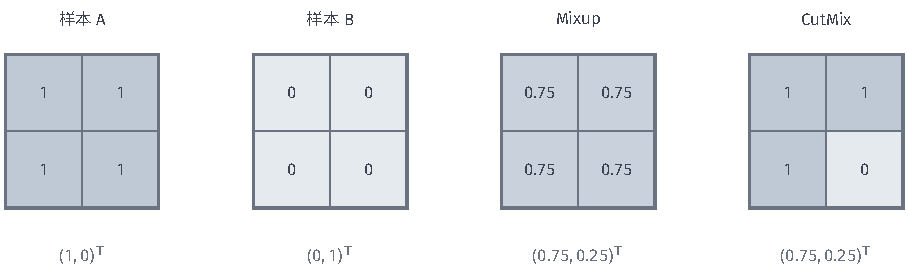
\includegraphics[width=153.793mm]{figures/03-models/02-neural-network-models/tikz/generalization-mixing/figure.pdf}
  \caption{构造的两类$2\times2$输入及其混合。样本A各位置为1，目标为$(1,0)^{\top}$；样本B各位置为0，目标为$(0,1)^{\top}$。Mixup取$\lambda=0.75$，各位置变为0.75；CutMix替换右下位置，保留面积也为0.75。二者目标均为$(0.75,0.25)^{\top}$，但空间组织不同。教学数值用于比较混合机制，类别也是构造的。}
  \label{fig:generalization-mixing}
\end{figure*}

混合强度、配对与目标共同规定这份函数约束。插值缺少任务意义时，线性标签会引入错误监督；类别线索集中在小区域时，面积也可能误表其贡献。保留真实任务语义的验证样本用来检验这些构造是否改善原任务。

\section{模型侧的泛化控制}
\label{sec:generalization-constraints}

同一结构的未绑定版本允许各位置分别选择参数，共享与绑定将其中某些自由度合并；范数惩罚则保留参数范围，在损失中增加尺度或稀疏偏好。前者规定可选计算，后者评价候选，两条路线分别接到第\ref{sec:generalization-capacity}节的归纳偏置与范数复杂度分析（参考\BookSectionRef{sec:network-norm-bounds}{第二卷“基础、理论和可信性”的“深度学习的可学习性”章“基于参数大小的可学习性”节}）。

这里按主要作用位置区分模型侧与训练侧：固定结构及显式损失项放在本节，更新收缩、随机训练扰动和轨迹选择放在第\ref{sec:generalization-training-process}节。方法在数学上可以联系，例如普通SGD中的L2梯度等价于特定收缩；具体实现据改变目标还是改变更新确定其作用位置。

\subsection{参数共享与参数绑定}
\label{sec:generalization-parameter-sharing}

相同局部关系出现在多个位置时，可以让这些位置共同估计一份规则。第\ref{sec:generalization-capacity}节的结构偏好在这里体现为参数相等：自由度减少，各次使用的梯度汇到同一参数，也同时要求这些位置采用同一变换。\term{参数共享}（parameter sharing）让不同计算位置使用同一参数对象。卷积核跨位置复用，循环权重跨时间复用；每次使用都贡献梯度，更新时累积到同一对象。\term{参数绑定}（weight tying）则强调多个模块的参数被限制为相等或具有指定对应关系，硬绑定常通过共享实现。

例如，词表嵌入矩阵$\bm E\in\mathbb R^{v\times d}$的第$j$行表示词元$j$，输出隐藏状态为$\bm h\in\mathbb R^d$时，可以绑定输出矩阵，令分数$\bm z=\bm E\bm h+\bm b$。这里要求输出隐藏宽度与嵌入宽度相容，输入和输出词表也有一致对应；不相容时需投影或另外定义绑定范围。绑定让同一词元的输入表示与输出判别共享信息，也减少独立参数，但同时施加两种职责可由同一表示承担的假设。

若不希望强制相等，可加入$\lambda\lVert\bm\theta_A-\bm\theta_B\rVert_2^2/2$，鼓励两组参数接近。有限$\lambda$下它们仍是两个参数对象，这是一种软约束。共享规定相等的参数结构，软约束在仍可不同的参数之间增加代价。任务若需要不同位置采用不同规则，过强绑定可能妨碍拟合。

\subsection{参数范数惩罚}
\label{sec:generalization-norm-penalties}

多组参数都能拟合已有样本时，可以在训练损失之外给它们不同评价。范数惩罚增加参数尺度代价，再与输入和分类间隔一起分析风险（参考\BookSectionRef{sec:network-norm-bounds}{第二卷“基础、理论和可信性”的“深度学习的可学习性”章“基于参数大小的可学习性”节}）。\term{范数惩罚}（norm penalty）将学习目标改为
\begin{equation}
  \min_{\bm\theta}\ \hat R_S(\bm\theta)+\lambda\Omega(\bm\theta),
  \qquad\lambda\geq0\text{。}
  \label{eq:generalization-regularized-objective}
\end{equation}
常见选择为$\Omega=\lVert\bm\theta\rVert_1$或$\Omega=\lVert\bm\theta\rVert_2^2/2$。后者惩罚范数的平方，实践中常简称L2正则化。它惩罚参数幅度，L1在0附近的非光滑形状则可以促成精确的零参数。

\begin{example}[L1与L2的收缩不同]
  \label{ex:generalization-shrinkage}
  对标量教学目标$\tfrac12(w-a)^2$，加入$\lambda w^2/2$后，最优解为$w=a/(1+\lambda)$；加入$\lambda|w|$后，最优解为$w=\operatorname{sign}(a)\max(|a|-\lambda,0)$。例如$a=0.4,\lambda=0.5$时，前者为$0.4/1.5$，后者为0。两个解析最优解显示惩罚形状的作用；神经网络的实际稀疏结果还取决于其目标与非光滑求解方法。
\end{example}

如果要一起选择或去掉一组参数，可以采用$\Omega(\bm\theta)=\sum_g\lVert\bm\theta_g\rVert_2$，其中组$g$可能对应某个特征、神经元或通道，必要时再按组大小加权。组范数对整组是否为0产生偏好，与逐参数L1的稀疏形态不同。组的边界、是否重叠与大小权重共同定义实际惩罚。

L1与组范数的零点不可微，近端更新常能更直接处理其非光滑部分；L2则有梯度$\lambda\bm\theta$。参数尺度还受重参数化影响，例如ReLU网络中某层放大、下一层相应缩小可能保留函数但改变参数惩罚。相同函数因表示方式而有不同惩罚，分析和实现因而需要共同固定约束对象。系数及偏置、归一化参数是否参与，再决定额外代价作用于哪些自由度。

\section{训练侧的泛化控制}
\label{sec:generalization-training-process}

候选和显式损失确定后，还要选择何时停止、使用轨迹中的哪个状态、怎样更新以及施加什么扰动。这些选择改变同一数据上的学习过程，训练敏感性与选解偏好分别解释其中部分机制（参考\BookSectionRef{sec:algorithmic-stability}{第二卷“基础、理论和可信性”的“一般学习的可学习性”章“算法稳定性与可学习性”节}和\BookSectionRef{sec:implicit-bias}{第二卷“基础、理论和可信性”的“深度学习的可学习性”章“基于参数梯度更新的可学习性”节}）。验证风险用于比较学得候选的新数据表现。

下面先讨论停止、平均与优化器选择，再讨论权重衰减和随机扰动。权重衰减在更新中收缩参数，因此归入训练侧；Dropout及噪声按训练时的操作位置归类，也可以从随机计算的期望损失理解。期望损失联系目标，操作位置联系实现，两种描述可以用于同一方法。

\subsection{提前终止}
\label{sec:generalization-early-stopping}

训练损失还在下降时，验证损失可能已经开始升高。此时可以把沿同一数据训练的时长作为候选选择；相应光滑与抽样条件下，训练时间和步长总量也会进入稳定性界（参考\BookSectionRef{sec:sgd-stability}{第二卷“基础、理论和可信性”的“一般学习的可学习性”章“凸学习问题的随机梯度下降”小节}）。\term{提前终止}（early stopping）根据验证数据选择训练时刻，将训练轨迹上的参数位置当作候选模型。它需要规定评估指标、检查间隔、最小改善量和容忍窗口，并保存出现最佳验证表现时的参数。

例如，每训练一个轮次计算一次验证损失，若连续$p$次检查都没有超过阈值的改善，就停止并恢复已保存的最优参数。恢复参数与使用停止时刻的参数不同；继续训练还需相应恢复优化器和调度状态。随机验证增强、Dropout未关闭或BatchNorm模式错误，都可能让停止判断混入无关噪声。

图~\ref{fig:generalization-early-stopping}展示可能出现的曲线形状。真实曲线可能有多个起伏，短期变差后还可能改善。容忍窗口据噪声、调度与目标选择，决定要为后续改善等待多少计算。
\begin{figure}[htbp]
  \centering
  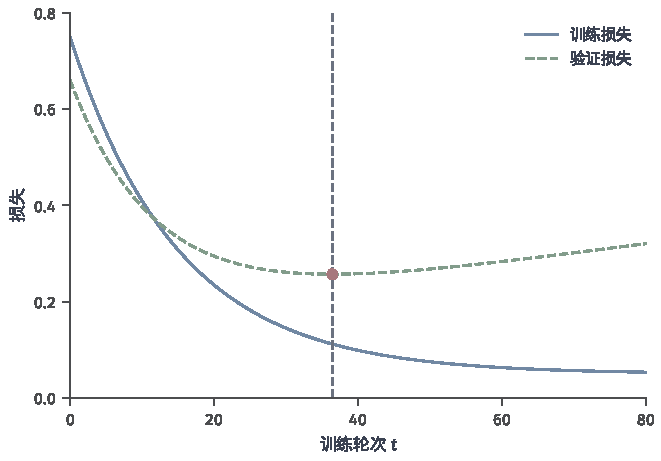
\includegraphics[width=105.412mm]{figures/03-models/02-neural-network-models/matplotlib/generalization-early-stopping/figure.pdf}
  \caption{提前终止的示意曲线。训练损失取$0.05+0.7\exp(-t/15)$，验证损失取$0.16+0.5\exp(-t/12)+0.002t$，$t$为训练轮次。虚线标出该构造验证函数的极小点附近，说明继续拟合与验证表现可能分离；这些函数仅用于讲解，不是实验记录。}
  \label{fig:generalization-early-stopping}
\end{figure}

在特定光滑、Lipschitz等条件下，SGD的稳定性界与步长总量和训练时间联系，解释持续更新怎样累积对样本的依赖（参考\BookSectionRef{sec:sgd-stability}{第二卷“基础、理论和可信性”的“一般学习的可学习性”章“凸学习问题的随机梯度下降”小节}）。实际停止仍在拟合进展和验证风险之间选择\scite{hardt2016sgd}

反复尝试停止策略时，验证集也在参与模型选择，所得方案可能适应这组数据的偶然差异。方案确定后再用最终测试评价。时间序列与持续感知还要模拟实际状态保留，让每个评价时刻只用当时可见的信息。

\subsection{参数平均}
\label{sec:generalization-weight-averaging}

更新噪声可能使训练后段的参数在附近波动，某个瞬时位置因而未必代表整段轨迹。参数平均综合这些位置，最后仍形成一个可直接推理的模型；平均位置的损失和验证表现确定这份综合是否合适。第\ref{sec:training-inexact-gradients}节说明了这些波动的来源。\term{指数移动平均}（exponential moving average, EMA）维护$\bar{\bm\theta}^{(t)}=\rho\bar{\bm\theta}^{(t-1)}+(1-\rho)\bm\theta^{(t)}$，$\rho\in[0,1)$。取初值为训练初始参数或当前参数可以避免零初值的缩小效应，$\rho$越大，对近期变化的响应越慢。推理时使用平均参数形成一个模型。

\term{随机权重平均}（stochastic weight averaging, SWA）选取训练后段的多个参数状态作算术平均。对已收集的$k$个状态，加入新状态$\bm\theta$时更新$\bar{\bm\theta}_{k+1}=k\bar{\bm\theta}_k/(k+1)+\bm\theta/(k+1)$。原始方案利用较大或周期性学习率采样训练后段区域，平均后若使用BatchNorm，还需按平均模型重新估计运行统计量\scite{izmailov2018swa}

参数坐标的平均要先经过网络计算，预测平均则组合已有输出。非线性映射通常不满足$f_{(\bm\theta_A+\bm\theta_B)/2}=(f_{\bm\theta_A}+f_{\bm\theta_B})/2$。同一轨迹附近的参数具有较一致的坐标含义，平均可能仍处在低损失区；独立模型的隐藏单元置换或尺度差异则可能把平均送到其他函数。

\begin{example}[等价网络的参数平均可以失效]
  \label{ex:generalization-parameter-average}
  取无偏置的两单元ReLU网络$f(x)=\operatorname{ReLU}(x)+\operatorname{ReLU}(-x)=|x|$。网络A的输入权重为$(1,-1)$，输出权重为$(1,1)$；网络B只交换两个隐藏单元，输入权重为$(-1,1)$，输出权重仍为$(1,1)$。两个网络的函数完全相同，但逐坐标平均后的输入权重为$(0,0)$，输出恒为0。预测平均仍给出$|x|$。
\end{example}

EMA和SWA在训练参数之外维护一份平均参数，推理使用这一个函数。它们综合同一轨迹，独立训练模型的预测集成则使用另一组函数；平均位置的偏差与实际验证风险仍据该模型评价。

\subsection{优化算法的隐式偏差}
\label{sec:generalization-implicit-bias}

同一目标有多个低损失解时，更新方向使轨迹倾向其中某些解。\term{隐式偏差}（implicit bias）描述学习过程形成的这种选择偏好；小批量无偏则描述梯度估计的期望。即使损失没有附加惩罚，线性和矩阵学习中的更新也可以产生特定偏好（参考\BookSectionRef{sec:implicit-bias}{第二卷“基础、理论和可信性”的“深度学习的可学习性”章“基于参数梯度更新的可学习性”节}）。

可分线性二分类提供一个明确结果：对$y_i\in\{-1,1\}$、无显式惩罚的逻辑损失，在相应步长与可分条件下，梯度下降使$\lVert\bm w\rVert_2$不断增长，方向趋向欧氏最大间隔分隔方向。这份经验逻辑损失的下确界为0，有限范数下达不到它；更新仍选择特定方向（条件与推导参考\BookSectionRef{sec:implicit-bias}{第二卷“基础、理论和可信性”的“深度学习的可学习性”章“基于参数梯度更新的可学习性”节}）\scite{soudry2018implicit}

\begin{example}[改变更新几何会改变选出的解]
  \label{ex:generalization-update-geometry}
  用一个训练样本拟合$w_1+2w_2=1$，目标为$\tfrac12(w_1+2w_2-1)^2$。从零初始化出发，足够小的固定步长梯度下降始终沿$(1,2)^{\top}$移动，收敛到$(1/5,2/5)^{\top}$，这是欧氏最小范数解。若改为固定预条件$\bm P=\operatorname{diag}(4,1)$，更新始终沿$(4,2)^{\top}$移动，则收敛到$(1/2,1/4)^{\top}$。两个解的训练误差都为0，后者最小化的是$\bm w^{\top}\bm P^{-1}\bm w$。未来数据若需要不同坐标承担不同作用，二者的风险也可能不同，哪种偏好适用要由未来输入与目标关系决定。
\end{example}

深度网络的选解偏好还随参数化、初始化、学习率、批量与时长改变，优化器比较因而需要固定网络与任务，并明确这些训练选择。Wilson等给出了自适应方法与GD／SGD选出不同解的构造，并在所研究的网络中观察到自适应方法训练更好而测试更差。这提供了比较非自适应与自适应更新的理由，结论限于相应设置\scite{wilson2017adaptive}

Choi等发现，优化器排名随超参数搜索范围和调节预算改变。比较时给不同方法各自调节参数，并使搜索预算相当；相同学习率数值在不同更新规则下可以产生不同位移。AdamW又含解耦衰减，更新方向与参数收缩都进入实际方案\scite{choi2020optimizers}

下面的比较过程用来检验当前任务中的选解差异：
\begin{enumerate}
  \item 固定网络、数据划分、增强与损失，以带动量SGD和AdamW作为两种候选。已有训练方案能稳定拟合时，先保留其为基准；更换优化器是检验不同更新几何的一种方式。
  \item 分别调节学习率、调度、动量或矩系数，以及适用的衰减系数。给两类候选相当的搜索与训练预算，记录达到目标训练损失的成本和验证表现。
  \item 联合阅读训练与验证曲线。训练误差仍高时，先排查第\ref{chap:neural-network-training}章的优化困难；训练相近而验证明显不同，才更便于判断不同训练规则带来的预测差异。固定时间预算的表现也应单独报告，因为慢方法可能尚未完成拟合。
  \item 对有希望的配置使用多个随机种子复核，再用验证结果选择。停止时刻、批量和参数平均也会改变轨迹，可以分别作控制实验；方案确定之后再做最终测试。
\end{enumerate}

代表性验证数据和多次训练支持某配置时，可以在该任务上采用它，结论随这份网络、数据和预算保留。中途从AdamW切到SGD会改变方向形成和状态含义；学习率、旧状态的丢弃或转换及切换时刻共同定义新方案，再由验证比较其效果。

参数平坦性描述指定坐标与扰动尺度内的损失变化，保持函数不变的重缩放也可以改变这一曲率。用它评价选解时，需固定坐标和尺度，或明确处理重参数化的方法，再将指标与当前任务的未来风险比较\scite{dinh2017sharp}

\subsection{邻域最坏损失与SAM}
\label{sec:generalization-sam}

在当前参数附近移动后损失迅速升高时，可以要求模型连同该邻域一起保持较低损失。指定坐标、范数和正半径后，用邻域内最大的损失作为外层目标。\term{锐度感知最小化}（sharpness-aware minimization, SAM）考虑
\begin{equation}
  \min_{\bm w}\ \max_{\lVert\bm\epsilon\rVert_2\leq\rho}
    \mathcal L(\bm w+\bm\epsilon)\text{。}
  \label{eq:generalization-sam}
\end{equation}
对内层目标在$\bm w$处作一阶近似且$\nabla\mathcal L(\bm w)\ne\bm0$时，欧氏球上的近似最大化点为
\[
  \bm\epsilon^\star
  =\rho\frac{\nabla\mathcal L(\bm w)}
              {\lVert\nabla\mathcal L(\bm w)\rVert_2}\text{。}
\]
随后在扰动点计算梯度，却把更新施加到原参数：$\bm w^+=\bm w-\eta\nabla\mathcal L(\bm w+\bm\epsilon^\star)$。图~\ref{fig:generalization-sam}把这两个步骤分开：红箭头寻找邻域内的高损失方向，绿色箭头读取该处梯度，却移动原参数。实际小批量实现常用同一批数据完成两次前后向；零梯度时的处理、归一化层状态、扰动范数和参数分组共同定义这两次计算。
\begin{figure*}[htbp]
  \centering
  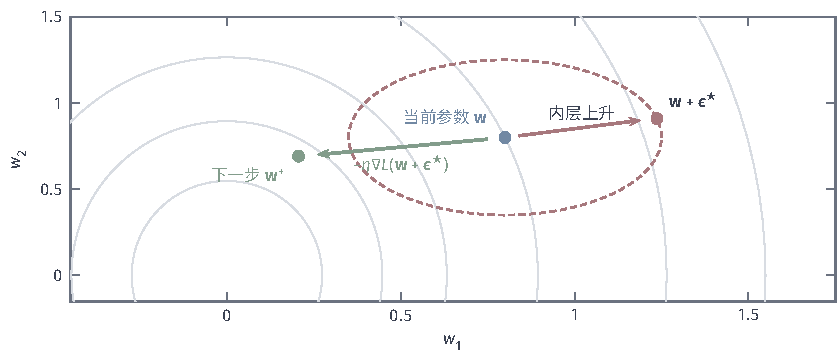
\includegraphics[width=142.275mm]{figures/03-models/02-neural-network-models/tikz/generalization-sam/figure.pdf}
  \caption{SAM一次近似更新的几何过程。灰线为教学目标$L(\bm w)=(4w_1^2+w_2^2)/2$的等高线，红色虚线是以当前参数为中心、半径$\rho=0.45$的扰动邻域。红箭头沿当前梯度的一阶近似到达边界高损失点，绿色箭头使用该扰动点的梯度更新原参数。图示说明两次梯度读取及更新的位置；内层只采用一阶近似，泛化效果另在任务上评价。}
  \label{fig:generalization-sam}
\end{figure*}

SAM在指定参数坐标和范数下改变邻域目标，重参数化也会改变同一函数的扰动集合。$\rho$很小时更新接近普通梯度，较大时一阶近似可能失准或妨碍拟合。这里扰动参数，输入鲁棒训练则扰动样本，两者评价的邻域不同。两次前后向的成本、训练拟合与独立验证风险一起说明该目标是否适合当前任务\scite{foret2021sam}

\subsection{权重衰减}
\label{sec:generalization-weight-decay}

当前位置的梯度给出数据损失方向，还可以在同一次更新中缩小参数幅度。\term{权重衰减}（weight decay）直接加入这种参数收缩；通常将学习率与衰减系数的乘积限制在零与一之间。第\ref{sec:training-optimizers}节的方向、尺度与历史状态共同决定它是否等价于损失中的范数惩罚。对无动量的普通SGD，L2惩罚更新为
\begin{equation}
  \bm\theta^{(t)}=\bm\theta^{(t-1)}-
    \eta_t(\bm g^{(t)}+\lambda\bm\theta^{(t-1)})
  =(1-\eta_t\lambda)\bm\theta^{(t-1)}-\eta_t\bm g^{(t)}\text{。}
  \label{eq:generalization-sgd-weight-decay}
\end{equation}
因而在相同参数范围及系数约定下，L2惩罚与学习率乘以$\lambda$的收缩等价。若所谓“衰减系数”直接表示每步乘法系数，就还需对应学习率；加入动量后，惩罚是否进入缓冲会改变下一步方向，等价关系据该实现重新对应。

对预条件矩阵$\bm P^{(t)}$，惩罚项进入梯度后产生$-\eta_t\lambda\bm P^{(t)}\bm\theta$，而解耦收缩产生$-\eta_t\lambda\bm\theta$。二者通常不同，Adam中惩罚还可能进入一阶、二阶矩统计。\term{AdamW}将衰减从自适应梯度更新中分离，其基本更新为
\begin{equation}
  \bm\theta^{(t)}=(1-\eta_t\lambda)\bm\theta^{(t-1)}-
    \eta_t\frac{\hat{\bm m}^{(t)}}{\sqrt{\hat{\bm v}^{(t)}}+\epsilon}\text{，}
  \label{eq:generalization-adamw}
\end{equation}
这里矩统计来自数据损失梯度，具体计算见式\eqref{eq:training-adam}\scite{loshchilov2019adamw}

衰减通过多步乘积发生，学习率调度、更新次数和是否排除部分参数都会改变总收缩量。解耦项按原参数直接收缩，预条件后的惩罚梯度则使用另一个方向。比较强度时同时固定更新规则与系数含义。

\subsection{Dropout}
\label{sec:generalization-dropout}
\label{sec:generalization-stochastic-regularization}

分类器若总依赖同一组中间特征共同出现，可以在训练中随机屏蔽其中一些，要求剩余特征仍参与预测。共享参数由这些随机计算共同训练，因而接受不同可用路径下的监督。\term{Dropout}在训练时随机屏蔽部分激活，使网络在不同的可用特征子集上完成同一任务。设隐藏表示为$\bm h$，各元素独立保留概率为$q\in(0,1]$，$m_j\sim\operatorname{Bernoulli}(q)$。常见的反向缩放形式为
\begin{equation}
  \tilde h_j=\frac{m_j}{q}h_j,\qquad
  \mathbb E[\tilde h_j\mid\bm h]=h_j,\qquad
  \operatorname{Var}(\tilde h_j\mid\bm h)=\frac{1-q}{q}h_j^2\text{。}
  \label{eq:generalization-dropout}
\end{equation}
训练时除以$q$，常规推理时关闭屏蔽并直接使用$\bm h$。另一约定在训练时不缩放、推理时乘$q$，两者必须与实现一致。这里$q$为保留率，有些接口使用的是失活率$1-q$\scite{srivastava2014dropout}

训练目标包含对掩码的期望$\mathbb E_{\bm m}\ell(f_{\bm\theta,\bm m}(\bm x),y)$。各掩码产生的子网络共享参数，梯度共同更新同一组对象。隐藏表示的期望虽被保持，完整非线性映射一般不满足$\mathbb E_{\bm m}f_{\bm\theta,\bm m}=f_{\bm\theta}$；无掩码推理提供确定计算，对随机网络平均的解释采用近似。

图~\ref{fig:generalization-dropout}展示同一隐藏层的一个掩码样本。被屏蔽单元的输入参数仍保留，后续批量可以重新启用该路径。较低$q$增加扰动和方差，也可能损害拟合。BatchNorm与Dropout组合时，还需关注随机激活对运行统计的影响；序列模型中跨时间独立采样或共享掩码，则具有不同扰动结构。
\begin{figure}[htbp]
  \centering
  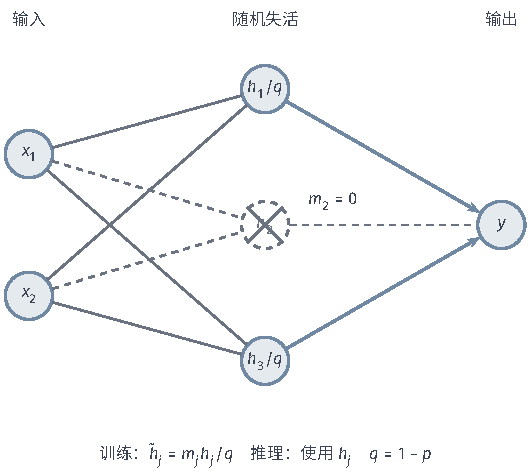
\includegraphics[width=89.793mm]{figures/03-models/02-neural-network-models/tikz/generalization-dropout/figure.pdf}
  \caption{一个三单元隐藏层的构造性Dropout示意。中间单元保留浅灰$h_2$轮廓并标出$m_2=0$，表示本批屏蔽的单元仍保留在模型中；灰色虚线为本次不参与前向计算的路径。底部公式带明确区分保留概率$q=1-p$与丢弃概率$p$，并给出inverted Dropout在训练时除以$q$、推理时无需再缩放的约定。}
  \label{fig:generalization-dropout}
\end{figure}

\subsection{结构化随机失活}
\label{sec:generalization-structured-dropout}

随机扰动应覆盖模型真正依赖的信息单位；若重复线索能从邻近位置轻易补回，逐元素屏蔽施加的约束就较弱。结构化随机失活根据网络结构选择连接、通道、空间块或整层作为屏蔽对象，使扰动粒度与第\ref{sec:training-connections}节的结构组织对应。

\term{DropConnect}对权重连接采样掩码，令$\tilde{\bm W}=\bm M\odot\bm W$，随后再计算激活；Dropout则直接作用于激活。基本训练与推理的缩放、分布近似应按各自约定处理，两种失活的随机函数不相同\scite{wan2013dropconnect}

\term{空间Dropout}（spatial dropout）在一个通道的所有空间位置使用同一掩码，削弱网络对某个整通道特征的依赖。\term{DropBlock}随机屏蔽特征图中连续的空间块，干扰局部邻域可提供的重复信息。多个块会重叠，边界也截掉部分位置，因此块中心的采样概率与最终元素失活比例需要分别计算\scite{ghiasi2018dropblock}

\term{随机深度}（stochastic depth）对残差分支随机启用或绕过，让训练时经过的有效深度变化。一个期望保持的实现写为$\bm h^{(l+1)}=\bm h^{(l)}+(m_l/q_l)F_l(\bm h^{(l)})$，$m_l\sim\operatorname{Bernoulli}(q_l)$，推理时使用全部分支。原始方法也可将缩放放在推理阶段；是否真正跳过被屏蔽分支的计算影响训练时间\scite{huang2016stochasticdepth}

连接、通道、空间块和整层使不同信息共同失活。小对象、窄通道或缺少恒等路径时，大块屏蔽可能直接去掉任务证据。保留概率、作用位置与掩码共享范围共同确定扰动，再据实际结构和验证结果选择其强度。

\subsection{噪声注入}
\label{sec:generalization-noise}

除保留或屏蔽之外，还可以连续改变表示或参数，在规定扰动分布下训练其平均表现。参数分布与期望损失提供这一描述的理论接口（参考\BookSectionRef{sec:parameter-distributions}{第二卷“基础、理论和可信性”的“深度学习的可学习性”章“基于参数分布的可学习性”节}）。\term{噪声注入}（noise injection）在训练中使用$\tilde{\bm h}=\bm h+\bm\epsilon$或$\tilde{\bm\theta}=\bm\theta+\bm\epsilon$，其中噪声的均值、协方差和采样范围需要明确。输入噪声属于数据增强的一种，中间表示噪声改变后续计算，参数噪声则同时影响所有使用该参数的位置。

对足够光滑的目标函数和小幅零均值噪声，二阶展开给出局部近似
\begin{equation}
  \mathbb E_{\bm\epsilon}[\mathcal L(\bm\theta+\bm\epsilon)]
  \approx\mathcal L(\bm\theta)+\tfrac12
      \operatorname{tr}(\bm\Sigma\nabla^2\mathcal L(\bm\theta))\text{，}
  \label{eq:generalization-noise-expansion}
\end{equation}
其中$\bm\Sigma=\mathbb E[\bm\epsilon\bm\epsilon^{\top}]$。噪声幅度与光滑条件控制余项，协方差与当前Hessian共同决定二阶项；非凸区域的负曲率还可能使该项为负。

一个可精确核查的特殊情况是线性回归。给定当前样本，对预测$\bm w^{\top}\bm x$、平方损失及输入噪声$\mathbb E\bm\epsilon=\bm0$、$\mathbb E\bm\epsilon\bm\epsilon^{\top}=\sigma^2\bm I$，有
\begin{equation}
  \mathbb E\tfrac12[y-\bm w^{\top}(\bm x+\bm\epsilon)]^2
  =\tfrac12(y-\bm w^{\top}\bm x)^2+\tfrac{\sigma^2}{2}\lVert\bm w\rVert_2^2\text{。}
  \label{eq:generalization-linear-noise}
\end{equation}
零均值消去交叉项，协方差决定额外二次项。这份精确联系来自线性预测、平方损失与输入噪声，改变模型、损失或注入位置后，期望目标需按新计算展开。

Dropout也可理解为一种乘性噪声：$\tilde h_j=h_j+[m_j/q-1]h_j$，条件均值为0、方差与$h_j^2$成比例。它与加性高斯噪声的分布和尺度不同。噪声是否符合任务中合理的变化，决定了对局部邻域的约束是否有意义；系统性错误标签或数据泄漏则仍需修正监督与数据组织。

\section{模型集成}
\label{sec:generalization-ensembles}

若不同训练过程保留了不同预测误差，可以通过组合预测减少其中部分波动。第\ref{sec:generalization-solution-selection}节的解差异在这里进入组合，成员质量与误差相关性共同决定效果。

\subsection{装袋法（Bagging）}
\label{sec:generalization-bagging}

\term{装袋法}（bootstrap aggregating, Bagging）从训练集多次自助重采样，分别训练成员，再组合预测，第\ref{sec:ensemble-bagging-bootstrap}节给出采样机制。变化的样本集合形成不同解，预测组合尝试减弱单次采样的影响。这里也关心学习过程的抽样敏感性，算法稳定性则在指定假设下分析替换样本对损失的影响（参考\BookSectionRef{sec:algorithmic-stability}{第二卷“基础、理论和可信性”的“一般学习的可学习性”章“算法稳定性与可学习性”节}）。用神经网络作为成员时，仍需保持相同的输出语义：回归平均数值预测，分类可平均类别概率或投票；概率平均通常不等于先平均分数再做Softmax。组合规则见第\ref{sec:ensemble-members-combination-output}节\scite{breiman1996bagging}

重采样的覆盖率和袋外预测分别由式\eqref{eq:ensemble-oob-probability}与式\eqref{eq:ensemble-oob-prediction}说明。神经网络的超参数和成员由验证选择，相关数据再按实际抽样单位重采样。例如按主体抽取体现主体变化，按窗口抽取则体现另一种随机过程。

集成收益还取决于成员之间共享多少波动。式\eqref{eq:ensemble-correlated-variance}在固定输入、等方差和等相关条件下，描述标量预测平均的方差，随机性来自训练集抽取、重采样及训练过程。共同波动在平均中继续保留，偏差还由成员的期望预测决定。这份标量预测方差公式解释波动，分类零一风险则还取决于目标与决策边界。

\subsection{基于训练随机性的集成}
\label{sec:generalization-randomness-ensemble}

初始化、数据次序、增强和随机失活在同一训练集上也能形成不同预测函数，来源见第\ref{sec:generalization-solution-selection}节。使用这些训练选择构建集成时，差异来自过程，成员可以使用相同原始样本。袋外集合则需要装袋法中未抽中的样本这一数据组织。

成员质量与差异共同进入组合。在关键输入上系统性错误的模型可能拖低预测，几乎相同的模型则保留共同误差。单模型表现、预测分歧与组合权重由同一验证方案比较，确定成员后再做最终测试。

集成通常增加训练和推理成本。$M$个相同规模网络若顺序运行，模型计算量约为单个的$M$倍；并行运行可以降低部分等待时间，却需要更多设备或存储。第\ref{sec:generalization-weight-averaging}节的参数平均形成一个模型，预测集成则保留多个模型；前者在平均参数上重新计算，后者组合已有输出，函数与部署成本都可能不同。成员数与组合规则据任务质量、延迟和资源预算共同选择。

\section{本章小结}
\label{sec:generalization-summary}

相同训练拟合可以依赖不同线索，未来使用时的风险因而需要连同数据覆盖、结构偏好与选解过程判断。同分布新样本、场景变化和持续状态各有评价条件，数据划分据实际使用方式组织。

增强把任务允许的变化写进经验目标，参数共享与范数惩罚引入结构和尺度偏好，权重衰减通过更新收缩参数，随机失活与噪声约束受扰动的计算，停止时刻和参数平均改变轨迹上的解选择，集成则利用多个预测的差异。组合时各自条件仍起作用：增强保持任务语义，约束保留所需规律，参数平均保持坐标对应，集成成员提供合适差异。复杂度、稳定性与隐式偏差解释其中不同环节，符合使用场景的验证与独立测试再检验完整方案。

\paragraph{扩展阅读}
Goodfellow等教材第7章讨论显式与隐式正则化；Mixup原论文展示如何把样本间的插值约束加入训练。阅读时可将增强的任务语义、更新路径与预测评价接在一起，辨认各结果使用的数据与条件\scite{goodfellow2016,zhang2018mixup}

